\documentclass[a4paper, 11pt]{report}

% --- PACCHETTI FONDAMENTALI ---
\usepackage[utf8]{inputenc}
\usepackage[T1]{fontenc}
\usepackage{lmodern}
\usepackage[english]{babel}
\usepackage{comment}

% Gestione Immagini e Grafica
\usepackage{graphicx}
\usepackage{float}       % Per forzare il posizionamento delle figure (H)
\usepackage{caption}     % Per gestire le didascalie
\DeclareCaptionFormat{nocaption}{} % Per gestire i notebook
\newcommand{\jupytercaptions}{\captionsetup{format=nocaption,aboveskip=0pt,belowskip=0pt}}
\graphicspath{{./figures/}} % Assicura che legga la cartella figures

% Matematica
\usepackage{amsmath}
\usepackage{amssymb}
\usepackage{amsfonts}
\usepackage{mathtools}

% Gestione Codice (Pygments/Listings)
% Se usi minted o listings nelle slide, assicurati che siano qui.
% Esempio generico per input di codice:
\usepackage{listings}
\usepackage{xcolor}

% Gestione Layout e Link
\usepackage[margin=2.5cm]{geometry} % Margini da dispensa
\usepackage{hyperref}    % Indice cliccabile e link
\usepackage{parskip}     % Spazio tra paragrafi invece dell'indentazione (più leggibile per dispense)
\usepackage{pdfpages} % Permette di includere file PDF esterni


\usepackage{fancyvrb}
\usepackage{xcolor}
\usepackage{textcomp} % Importante per certi simboli

% --- INIZIO DEFINIZIONI COMPLETE PYGMENTS ---
\makeatletter
\def\PY@reset{\let\PY@it=\relax \let\PY@bf=\relax%
    \let\PY@ul=\relax \let\PY@tc=\relax%
    \let\PY@bc=\relax \let\PY@ff=\relax}
\def\PY@tok#1{\csname PY@#1\endcsname}
\def\PY@toks#1+{\ifx\relax#1\empty\else%
    \PY@tok{#1}\expandafter\PY@toks\fi}
\def\PY@do#1{\PY@bc{\PY@tc{\PY@ul{%
    \PY@it{\PY@bf{\PY@ff{#1}}}}}}}
\def\PY#1#2{\PY@reset\PY@toks#1+\relax+\PY@do{#2}}

% --- Definizioni dei caratteri speciali (parentesi, backslash, ecc.) ---
\def\PYZbs{\char`\\}
\def\PYZus{\char`\_}
\def\PYZob{\char`\{}
\def\PYZcb{\char`\}}
\def\PYZca{\char`\^}
\def\PYZam{\char`\&}
\def\PYZlt{\char`\<}
\def\PYZgt{\char`\>}
\def\PYZsh{\char`\#}
\def\PYZpc{\char`\%}
\def\PYZdl{\char`\$}
\def\PYZhy{\char`\-}
\def\PYZsq{\textquotesingle}
\def\PYZdq{\char`\"}
\def\PYZti{\char`\~}
\def\PYZat{\char`\@}
\def\PYZlb{\char`\[}
\def\PYZrb{\char`\]}

% --- Stile dei colori (Default Style) ---
\expandafter\def\csname PY@k\endcsname{\let\PY@bf=\textbf\def\PY@tc##1{\textcolor[rgb]{0.00,0.50,0.00}{##1}}} % Keyword
\expandafter\def\csname PY@kp\endcsname{\def\PY@tc##1{\textcolor[rgb]{0.00,0.50,0.00}{##1}}} % Keyword.Pseudo
\expandafter\def\csname PY@kr\endcsname{\let\PY@bf=\textbf\def\PY@tc##1{\textcolor[rgb]{0.00,0.50,0.00}{##1}}} % Keyword.Reserved
\expandafter\def\csname PY@kt\endcsname{\def\PY@tc##1{\textcolor[rgb]{0.69,0.00,0.25}{##1}}} % Keyword.Type
\expandafter\def\csname PY@n\endcsname{\def\PY@tc##1{\textcolor[rgb]{0.00,0.00,0.00}{##1}}} % Name
\expandafter\def\csname PY@na\endcsname{\def\PY@tc##1{\textcolor[rgb]{0.49,0.56,0.16}{##1}}} % Name.Attribute
\expandafter\def\csname PY@nb\endcsname{\def\PY@tc##1{\textcolor[rgb]{0.00,0.50,0.00}{##1}}} % Name.Builtin
\expandafter\def\csname PY@nc\endcsname{\let\PY@bf=\textbf\def\PY@tc##1{\textcolor[rgb]{0.00,0.00,1.00}{##1}}} % Name.Class
\expandafter\def\csname PY@no\endcsname{\def\PY@tc##1{\textcolor[rgb]{0.53,0.00,0.00}{##1}}} % Name.Constant
\expandafter\def\csname PY@nd\endcsname{\def\PY@tc##1{\textcolor[rgb]{0.67,0.13,1.00}{##1}}} % Name.Decorator
\expandafter\def\csname PY@ni\endcsname{\let\PY@bf=\textbf\def\PY@tc##1{\textcolor[rgb]{0.47,0.47,0.47}{##1}}} % Name.Entity
\expandafter\def\csname PY@ne\endcsname{\let\PY@bf=\textbf\def\PY@tc##1{\textcolor[rgb]{0.82,0.25,0.23}{##1}}} % Name.Exception
\expandafter\def\csname PY@nf\endcsname{\def\PY@tc##1{\textcolor[rgb]{0.00,0.00,1.00}{##1}}} % Name.Function
\expandafter\def\csname PY@nn\endcsname{\let\PY@bf=\textbf\def\PY@tc##1{\textcolor[rgb]{0.00,0.00,1.00}{##1}}} % Name.Namespace
\expandafter\def\csname PY@nt\endcsname{\let\PY@bf=\textbf\def\PY@tc##1{\textcolor[rgb]{0.00,0.50,0.00}{##1}}} % Name.Tag
\expandafter\def\csname PY@nv\endcsname{\def\PY@tc##1{\textcolor[rgb]{0.10,0.09,0.49}{##1}}} % Name.Variable
\expandafter\def\csname PY@l\endcsname{\def\PY@tc##1{\textcolor[rgb]{0.73,0.38,0.84}{##1}}} % Literal
\expandafter\def\csname PY@m\endcsname{\def\PY@tc##1{\textcolor[rgb]{0.40,0.40,0.40}{##1}}} % Literal.Number
\expandafter\def\csname PY@mb\endcsname{\def\PY@tc##1{\textcolor[rgb]{0.40,0.40,0.40}{##1}}} % Literal.Number.Bin
\expandafter\def\csname PY@mf\endcsname{\def\PY@tc##1{\textcolor[rgb]{0.40,0.40,0.40}{##1}}} % Literal.Number.Float
\expandafter\def\csname PY@mh\endcsname{\def\PY@tc##1{\textcolor[rgb]{0.40,0.40,0.40}{##1}}} % Literal.Number.Hex
\expandafter\def\csname PY@mi\endcsname{\def\PY@tc##1{\textcolor[rgb]{0.40,0.40,0.40}{##1}}} % Literal.Number.Integer
\expandafter\def\csname PY@mo\endcsname{\def\PY@tc##1{\textcolor[rgb]{0.40,0.40,0.40}{##1}}} % Literal.Number.Oct
\expandafter\def\csname PY@s\endcsname{\def\PY@tc##1{\textcolor[rgb]{0.73,0.13,0.13}{##1}}} % Literal.String
\expandafter\def\csname PY@sb\endcsname{\def\PY@tc##1{\textcolor[rgb]{0.73,0.13,0.13}{##1}}} % Literal.String.Backtick
\expandafter\def\csname PY@sc\endcsname{\def\PY@tc##1{\textcolor[rgb]{0.73,0.13,0.13}{##1}}} % Literal.String.Char
\expandafter\def\csname PY@sd\endcsname{\def\PY@tc##1{\textcolor[rgb]{0.73,0.13,0.13}{##1}}} % Literal.String.Doc
\expandafter\def\csname PY@s2\endcsname{\def\PY@tc##1{\textcolor[rgb]{0.73,0.13,0.13}{##1}}} % Literal.String.Double
\expandafter\def\csname PY@se\endcsname{\let\PY@bf=\textbf\def\PY@tc##1{\textcolor[rgb]{0.73,0.40,0.13}{##1}}} % Literal.String.Escape
\expandafter\def\csname PY@sh\endcsname{\def\PY@tc##1{\textcolor[rgb]{0.73,0.13,0.13}{##1}}} % Literal.String.Heredoc
\expandafter\def\csname PY@si\endcsname{\let\PY@bf=\textbf\def\PY@tc##1{\textcolor[rgb]{0.73,0.40,0.53}{##1}}} % Literal.String.Interpol
\expandafter\def\csname PY@sx\endcsname{\def\PY@tc##1{\textcolor[rgb]{0.00,0.50,0.00}{##1}}} % Literal.String.Other
\expandafter\def\csname PY@sr\endcsname{\def\PY@tc##1{\textcolor[rgb]{0.73,0.40,0.53}{##1}}} % Literal.String.Regex
\expandafter\def\csname PY@s1\endcsname{\def\PY@tc##1{\textcolor[rgb]{0.73,0.13,0.13}{##1}}} % Literal.String.Single
\expandafter\def\csname PY@ss\endcsname{\def\PY@tc##1{\textcolor[rgb]{0.10,0.09,0.49}{##1}}} % Literal.String.Symbol
\expandafter\def\csname PY@c\endcsname{\let\PY@it=\textit\def\PY@tc##1{\textcolor[rgb]{0.25,0.50,0.50}{##1}}} % Comment
\expandafter\def\csname PY@cp\endcsname{\def\PY@tc##1{\textcolor[rgb]{0.74,0.48,0.00}{##1}}} % Comment.Preproc
\expandafter\def\csname PY@c1\endcsname{\let\PY@it=\textit\def\PY@tc##1{\textcolor[rgb]{0.25,0.50,0.50}{##1}}} % Comment.Single
\expandafter\def\csname PY@cs\endcsname{\let\PY@it=\textit\def\PY@tc##1{\textcolor[rgb]{0.25,0.50,0.50}{##1}}} % Comment.Special
\expandafter\def\csname PY@gd\endcsname{\def\PY@tc##1{\textcolor[rgb]{0.63,0.00,0.00}{##1}}} % Generic.Deleted
\expandafter\def\csname PY@ge\endcsname{\let\PY@it=\textit} % Generic.Emph
\expandafter\def\csname PY@gr\endcsname{\def\PY@tc##1{\textcolor[rgb]{1.00,0.00,0.00}{##1}}} % Generic.Error
\expandafter\def\csname PY@gh\endcsname{\let\PY@bf=\textbf\def\PY@tc##1{\textcolor[rgb]{0.00,0.00,0.50}{##1}}} % Generic.Heading
\expandafter\def\csname PY@gi\endcsname{\def\PY@tc##1{\textcolor[rgb]{0.00,0.63,0.00}{##1}}} % Generic.Inserted
\expandafter\def\csname PY@go\endcsname{\def\PY@tc##1{\textcolor[rgb]{0.53,0.53,0.53}{##1}}} % Generic.Output
\expandafter\def\csname PY@gp\endcsname{\def\PY@tc##1{\textcolor[rgb]{0.00,0.00,0.50}{##1}}} % Generic.Prompt
\expandafter\def\csname PY@gs\endcsname{\let\PY@bf=\textbf} % Generic.Strong
\expandafter\def\csname PY@gu\endcsname{\let\PY@bf=\textbf\def\PY@tc##1{\textcolor[rgb]{0.50,0.00,0.50}{##1}}} % Generic.Subheading
\expandafter\def\csname PY@gt\endcsname{\def\PY@tc##1{\textcolor[rgb]{0.00,0.27,0.87}{##1}}} % Generic.Traceback
\expandafter\def\csname PY@o\endcsname{\def\PY@tc##1{\textcolor[rgb]{0.40,0.40,0.40}{##1}}} % Operator
\expandafter\def\csname PY@ow\endcsname{\let\PY@bf=\textbf\def\PY@tc##1{\textcolor[rgb]{0.67,0.13,1.00}{##1}}} % Operator.Word
\makeatother
% --- FINE DEFINIZIONI PYGMENTS ---

% ------------------

\title{\textbf{Computing Methods for Experimental Physics and Data Analysis} \\
\vspace{0.5em}
{\large Notes adjusted from the 2025-26 course slides and lessons}}
\author{Lorenzo Nepi}
\date{\today}

\begin{document}

\maketitle

\newpage
\thispagestyle{empty}
\null
\newpage

\tableofcontents

\newpage

% -------------------------------------------------------------------
% PART I: BASICS
% -------------------------------------------------------------------
\chapter[Python basics]{Python basics \\[0.5ex] \large \textit{(Prof. Baldini)}}


%\begin{comment}
\section{Development workflow: the necessity of version control}

\subsection{Introduction}
Most of us would agree that research should be \textbf{correct} \emph{and} \textbf{reproducible} \footnote{"Reproducible": \emph{able to be shown, done, or made.} Source: the Cambridge Dictionary}.
Reproducible research is, for example, data analysis that starts with the raw data and arrives at the same answers. Software plays a paramount role in modern experimental physics and therefore it is a crucial ingredient in reproducibility of research and it should be developed under controlled conditions, just like the experiments are performed. \textit{Oftentimes, physicists are better at correctness than reproducibility}. Scientists are famous for producing poor-quality software and the community is lagging behind on the best practices that are ubiquitous among professional software development (and there are many good reasons why that is the case). 

Consider the last piece of analysis software you have written. Would somebody else be able to use it without your help? Would it run as is on somebody else's computer? Would you be able to adapt it for somebody else's computer? Would you be able to run it on your computer a year from now?
Not to mention efficiency: could your software run significantly faster? And if so: would you care?

And now take the last paper that you have read.  Would it be possible to re-do the analysis (obtaining the same results)? Have the raw data been preserved in a readable format? Is the analysis software still available? Is there still somebody around understanding what the software does? Are there machines around that can run the analysis software? Is the software even version-controlled?

Standards sometimes help (e.g. the \href{https://fits.gsfc.nasa.gov/fits\_standard.html}{FITS} standard for astronomical data) however, they often hinder performance (e.g., compared to ROOT, FITS I/O is horrible by any reasonable metrics\footnote{This comment was on the lesson slides and, as a humble student, I reported it as is. However, I would like to peacefully disagree. For me ROOT enters by birthright in the realm of "complicazione affari semplici"}).

Most modern experiments are run by large teams, like the LHC Collaborations which count thousands of members. How do you handle development in such an environment? How do you distribute the source code? How do you know which version any single person is running? How do hundreds of people develop the same code concurrently? How do you make sure that your last awesome change isn't breaking everybody else's code?

And even if you work in a small team, how do you exchange code with your collaborators? How do you collect feedback? How do you distribute updates? And even if you are working by yourself, why is the thing giving a different answer with respect to the last time you ran it last week? And which is the correct answer?

These questions are all fundamental in the research world, and you will be able to give a satisfying answer to most of them once you have mastered \textit{version control}. 

\subsection{Version control}

Here is a dictionary definition of \textbf{version control}: \emph{A component of software configuration management, version control, also known as revision control or source control, is the management of changes to documents, computer programs, large web sites, and other collections of information\footnote{Source: Wikipedia}.} In other words, you need to collect meta-data (how, when, where, by whom and why?) whenever the code is changed and freeze forever a specific configuration of the code-base. In doing so, it becomes a lot easier to find and fix bugs, develop the same code in collaboration with others and keep track of your progress. Keep in mind: \textbf{version control is a necessity in modern science}. 

\subsection{Version Control Systems (VCS) and practices}
Here is some basic terminology regarding version control:
\begin{itemize}
    \item[-] \textbf{Repository}: the place where files' current and historical data are stored.
    \item[-] \textbf{Revision or version}: the state at a point in time of the entire tree in the repository.
    \item[-] \textbf{Clone}: creating a repository containing the revisions from another repository.
    \item[-] \textbf{Working copy}: a local copy of files from a repository at a specific revision.
    \item[-] \textbf{Checkout}: create a local working copy from the repository.
    \item[-] \textbf{Change or diff}: a specific modification to a set of files under version control.
    \item[-] \textbf{Commit}: write the changes made in the working copy back to the repository.
\end{itemize}
Next, we will explore the fundamental architectures of different version control systems.

\textbf{Local Version Control Systems (e.g., RCS)}
\begin{center}
    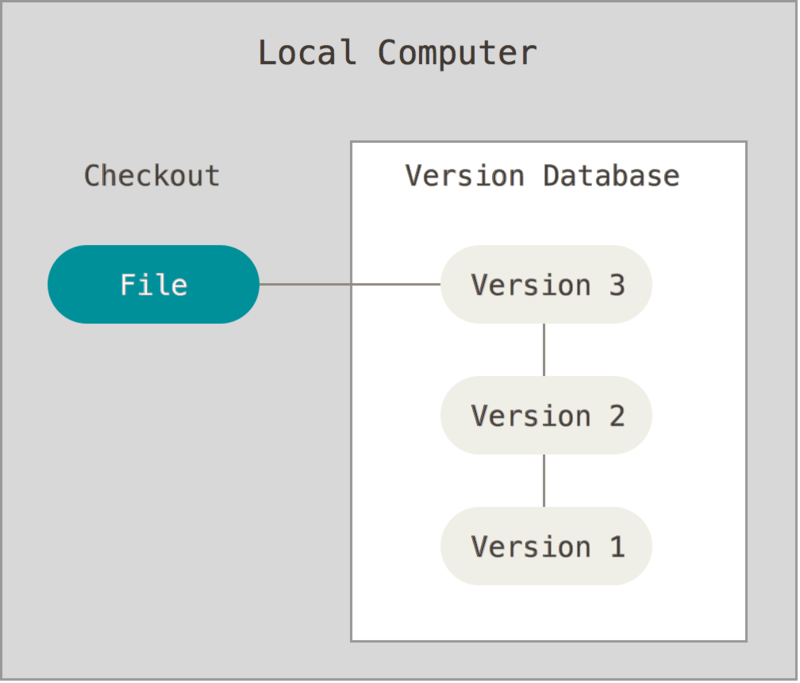
\includegraphics[width=0.35\textwidth]{vcs_local}
\end{center}
Local systems operate by storing only the incremental differences between file revisions in a local database. This approach efficiently minimizes disk space usage while guaranteeing that any previous state of a file can be accurately reconstructed on demand.

\textbf{Centralized Version Control Systems (e.g., CVS, Subversion)}
\begin{center}
    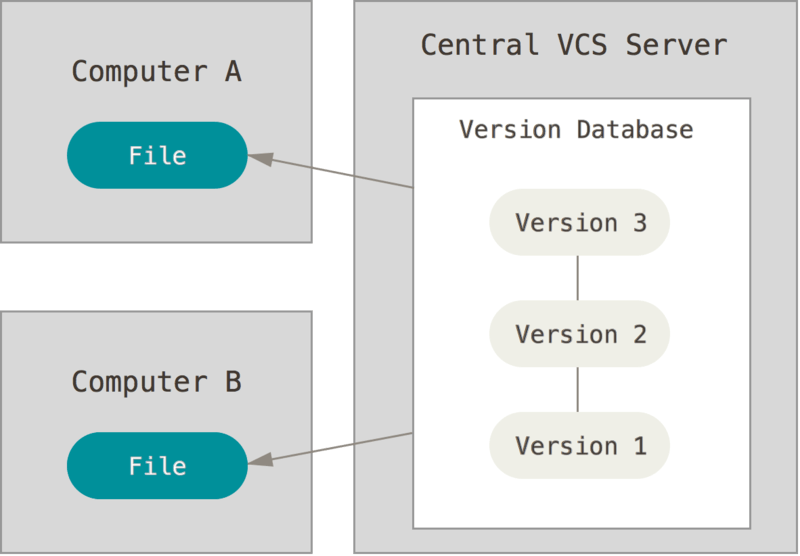
\includegraphics[width=0.35\textwidth]{vcs_centralized}
\end{center}
Centralized architectures rely on a single, dedicated server that contains all versioned files, from which clients check out a specific working copy. Dominant throughout the 1990s, this model follows a straightforward workflow:
\begin{itemize}
    \item[-] Check out a local working copy from the remote server;
    \item[-] Modify the working copy locally;
    \item[-] Commit the changes directly back to the central repository.
\end{itemize}

\textbf{Distributed Version Control Systems (e.g., Git, Mercurial)}
\begin{center}
    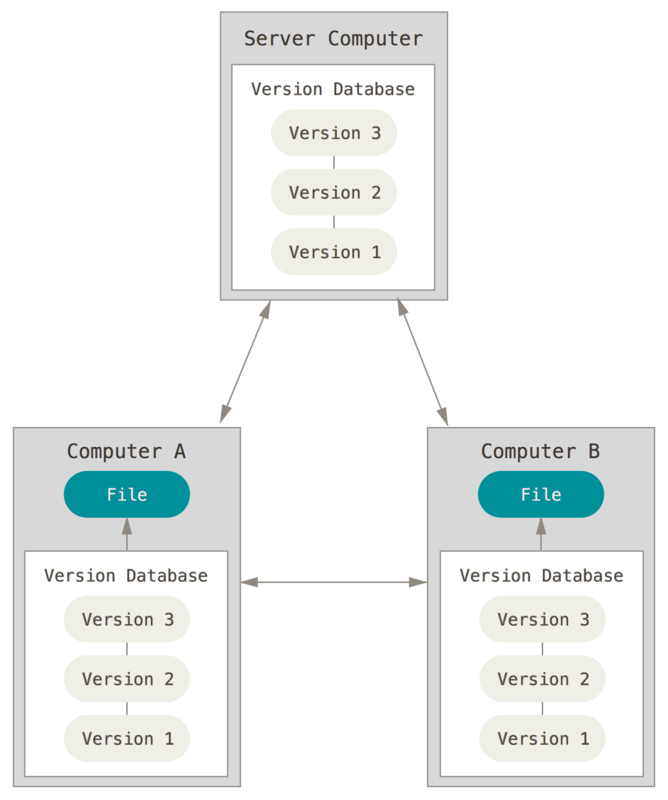
\includegraphics[width=0.35\textwidth]{vcs_distributed}
\end{center}
In a distributed system, clients do not just check out the latest snapshot; they fully mirror the entire repository along with its complete version history. This decentralized structure provides an inherent backup against server failures and enables a much richer, highly flexible variety of collaboration workflows.

\hrulefill

\subsection{Digression: hash functions}
\begin{center}
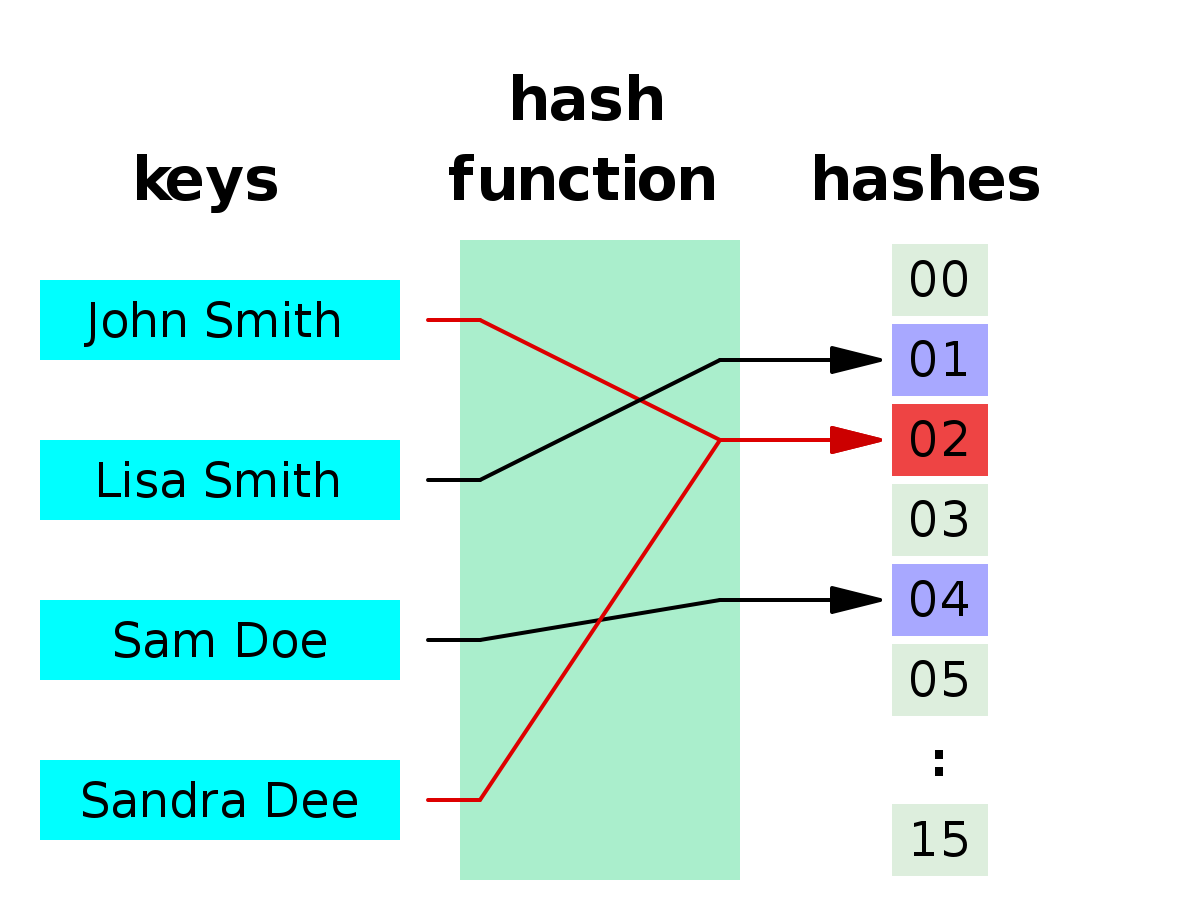
\includegraphics[width=0.5\textwidth]{hash}
\end{center}

Ever heard of checksums? Or short versions of Doodle links? A \textbf{hash function} maps data of arbitrary size to fixed-size values, e.g., anything to an integer. Hash functions should be \textit{deterministic} (uniform in the image space, to minimize collisions), fast to calculate and, possibly, hard to invert.

For example, every \emph{immutable} object is hashable in Python. Each type gets its own algorithm, as shown in the following example.

\input{pygments/hashing}

As said, in distributed VCS each commit gets its own hash. The following command returns the hash of the current commit in git (see below).

\begin{verbatim}
[lbaldini@nbbaldini slides]$ git rev-parse HEAD
e0a170d789865179d99506c9f067f3875292524b
\end{verbatim}

\hrulefill

\subsection{git}
Today \textbf{git} is the standard for VCS all across the world. At the following link you will find a complete introduction on how to set up your first git repository using GitHub: \\ \url{https://lucabaldini.github.io/metarep/setup.html}.
You will be able to fully understand the content at this URL after you have taken a look at the Advanced chapter.
\\
You will be introduced to git and GitHub during the in-person classes. Here we will just sum-up some of the basic concepts and commands.  

Let's start with some more definitions:
\begin{itemize}
    \item[-] \textbf{Branches}: alternative paths where more copies of the same files develop in different ways independently.
    \item[-] \textbf{Main}, or \textbf{master}, or \textbf{trunk}, or \textbf{tip}: the default primary branch of a repository.
    \item[-] \textbf{Merge}: application of two sets of changes to a set of files.
    \item[-] \textbf{Conflict}: changes to the same file by two or more developers that the system is unable to reconcile.
\end{itemize}
\begin{center}
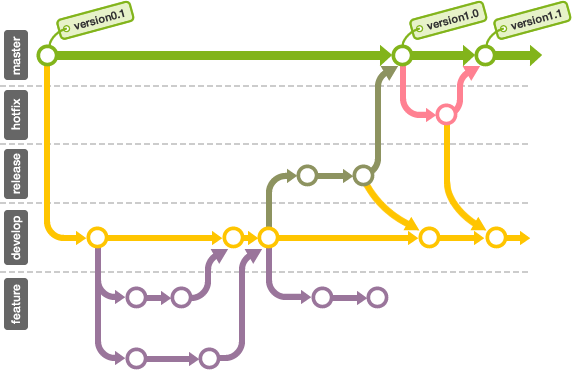
\includegraphics[width=0.5\textwidth]{vcs_workflow}
\end{center}
By typing \texttt{git -{}-help} in your terminal you will obtain the following list of commands: 
\begin{verbatim}
start a working area (see also: git help tutorial)
   clone      Clone a repository into a new directory

work on the current change (see also: git help everyday)
   add        Add file contents to the index
   mv         Move or rename a file, a directory, or a symlink
   rm         Remove files from the working tree and from the index

examine the history and state (see also: git help revisions)
   log        Show commit logs
   show       Show various types of objects
   status     Show the working tree status

grow, mark and tweak your common history
   branch     List, create, or delete branches
   checkout   Switch branches or restore working tree files
   commit     Record changes to the repository
   diff       Show changes between commits, commit and working tree, etc
   merge      Join two or more development histories together
   tag        Create, list, delete or verify a tag object signed with GPG

collaborate (see also: git help workflows)
   pull       Fetch from and integrate with another repository or a local branch
   push       Update remote refs along with associated objects
\end{verbatim}

Here's an example of a simple but realistic work-flow you should be following while coding:
\begin{enumerate}
    \item Clone your repository
    \item Create a new branch and check it out
    \item Do all you have to do
    \item Add the new files, commit your modified files
    \item Create a pull request
    \item Have your pull request reviewed
    \item Merge the branch on the master
    \item Tag the master
\end{enumerate}

You should always pick a sensible name for your branches. Try and express your \emph{intent}. \\ Examples of bad names: \verb|my_branch|, \verb|new_branch|, \verb|awesome_branch| \\ Examples of reasonable names: \verb|update_data_format|, \verb|fix_issue_2376|.

Try and isolate related changes in the smallest possible subset. Attack one problem at a time. Do not mix unrelated issues in the same pull request: the smaller the pull request, the easier the review.

\textbf{Don't try to do the work that the VCS is supposed to do}. Do not keep around multiple copies of the same file with a different suffix - the VCS is keeping track of the changes. Do not copy and paste a block of code, comment the original and edit the second - this will make diffs (differences) easier to understand.

VCSs are good at handling text files. Do not commit large binary files (e.g., data sets) to your repository because they will stay there forever.

\subsubsection{Typical layout of a Python package}
Say you have a project called "sample". Here is how the repository layout should look like if you follow the right conventions:

\begin{Verbatim}
.
|-- README.rst
|-- LICENSE
|-- setup.py
|-- requirements.txt
|-- sample/
|   |-- __init__.py
|   |-- core.py
|   `-- helpers.py
|-- docs/
|   |-- conf.py
|   `-- index.rst
`-- tests/
    |-- test_basic.py
    `-- test_advanced.py
\end{Verbatim}

This directory tree reproduces the structure of your GitHub repository. You can find:

\begin{itemize}
    \item[-] a README.rst file
    \item[-] a LICENSE (when in doubt use GPL v3)
    \item[-] a requirements.txt file (dependencies, for pip)
    \item[-] the sample directory (actual python code. Note: it's the same name as the project)
    \item[-] docs (directory with documentation)
    \item[-] tests (directory with unit tests)
\end{itemize}
We shall talk a lot about installation, documentation and unit tests in the advanced module.

Now, this was a very brief introduction to version control and git. The best way to learn how to use these instruments is to work with them directly, so if you have the occasion, try to create your own repository on GitHub. To do that, follow the instructions in the first chapter ("Repository setup") of this document: \url{https://lucabaldini.github.io/metarep/setup.html}.

\hrulefill

{\footnotesize
\underline{Conversations with Master Shifu, part 1:}

\begin{itemize}
    \item[-] "What is version control?" \textit{Welcome to this class!}
    \item[-] "I heard about such thing, but I don't need it." \textit{If you really think so, you do need it but don't know yet!}
    \item[-] "Every once in a while I create a copy of a file with a \texttt{\_vn} appended. Or I periodically create an archive and attach a version number to it." \textit{And how is that helpful when something goes wrong?}
    \item[-] "I created my own custom-made system." \textit{Mhhh\ldots suspicious... git was written by Linus Torvalds}.
    \item[-] I do use a professional tool for the job (e.g., git). \textit{Congratulations: you are a person of good taste!}
    \item[-] "Which VCS should I use?" \textit{Everybody else is using git, these days---you might as well stick to that.}
    \item[-] "Shall I set up a server myself or use a hosting service?" \textit{This is a no brainer: use a service (e.g., GitHub, GitLab, Bitbucket)}.
    \item[-] "What shall I use version control for?" \textit{Your thesis. Your papers (or lab assignments). Your webpage (if you have one). The invitations for your wedding. Really: everything you care about!}
    \item[-] "Shall I care about the license?" \textit{Definitely: make it easy for others to use and adapt your code (unless you have good reasons not to). GNU General Public License v3.0 is a good choice for code. Creative Commons Attribution-ShareAlike 4.0 is a good choice for documents.}
\end{itemize} }

\hrulefill

\subsection{References}
\begin{itemize}
    \item[-] \url{https://en.wikipedia.org/wiki/Version_control}
    \item[-] \url{https://git-scm.com/book/en/v2/Getting-Started-About-Version-Control}
    \item[-] \url{https://en.wikipedia.org/wiki/Hash_function}
    \item[-] \url{https://git-scm.com/}
    \item[-] \url{https://github.com/}
    \item[-] \url{https://bitbucket.org/}
    \item[-] \url{https://about.gitlab.com/}
    \item[-] \url{https://pubs.acs.org/doi/10.1021/acs.orglett.9b03216}
    \item[-] \url{https://www.nature.com/articles/s41586-020-2649-2}
    \item[-] \url{http://www.jarrodmillman.com/publications/millman2014developing.pdf}
\end{itemize}

\section{Python Basics (1/2)}

\subsection{Coding conventions and the Zen of Python}

\emph{Coding conventions} are guidelines about how to write code that vary across different languages. You are encouraged to stick to them, but your code will happily run even if you don't. \\
So, why should you care? \textit{Code is read much more often than it is written.}

In the Python ecosystem, this philosophy of readability and elegance is beautifully encapsulated in the ``Zen of Python'' (PEP 20, \url{https://www.python.org/dev/peps/pep-0020/}). It is a collection of 19 guiding principles that dictate the design of the language itself and help developers write clean, ``Pythonic'' code. You can reveal these aphorisms at any time directly from the interpreter:

\begin{verbatim}
[lbaldini@nbbaldini slides]$ python
Python 3.7.4 (default, Jul  9 2019, 16:32:37)
[GCC 9.1.1 20190503 (Red Hat 9.1.1-1)] on linux
Type "help", "copyright", "credits" or "license" for more information.
>>> import this
The Zen of Python, by Tim Peters

Beautiful is better than ugly.
Explicit is better than implicit.
Simple is better than complex.
Complex is better than complicated.
Flat is better than nested.
Sparse is better than dense.
Readability counts.
Special cases aren't special enough to break the rules.
Although practicality beats purity.
Errors should never pass silently.
Unless explicitly silenced.
In the face of ambiguity, refuse the temptation to guess.
There should be one-- and preferably only one --obvious way to do it.
Although that way may not be obvious at first unless you're Dutch.
Now is better than never.
Although never is often better than *right* now.
If the implementation is hard to explain, it's a bad idea.
If the implementation is easy to explain, it may be a good idea.
Namespaces are one honking great idea -- let's do more of those!
\end{verbatim}

As the Zen explicitly reminds us: \textit{readability counts}. Therefore, a good one-line summary for coding conventions is: \textbf{think about following them, but don't be obsessed by them}.

The bible of coding conventions for Python is the \textbf{PEP 8 Style Guide for Python Code}, which you can find at the following link: \url{https://www.python.org/dev/peps/pep-0008/}. There are automatic tools out there to help you:
\begin{itemize}
    \item[-] pylint: \url{https://www.pylint.org/}
    \item[-] Pyflakes: \url{https://pypi.org/project/pyflakes/}
    \item[-] mypy: \url{http://mypy-lang.org/}
    \item[-] pycodestyle: \url{https://github.com/PyCQA/pycodestyle}
\end{itemize}

The following section contains an introduction to some basic Python coding. Of course, being able to code a little is a prerequisite of the course, but you may not be familiar with some of these concepts and conventions. So read the code, understand what it does and see if you remember everything you need for this course.

\subsection{Python basics (through code)}
\subsubsection{- Variables and basic types}
\input{pygments/basic_types}

\subsubsection{- Digression: string formatting}
\input{pygments/string_formatting}

Here are some string formatting tips in a nutshell:
\begin{itemize}
    \item[-] Never add strings.
    \item[-] Try to avoid using the \texttt{\%} operator.
    \item[-] \texttt{format()} is ok, although a little bit on the verbose side.
    \item[-] Use f-strings whenever you can (need Python 3.6+).
\end{itemize}

\subsubsection{- Defining functions}
\textit{DRY (Don't Repeat Yourself) is better than WET (Write Every Time)}.
The \textbf{DRY} principle is stated as "Every piece of knowledge must have a single, unambiguous, authoritative representation within a system" \footnote{Source: \url{https://en.wikipedia.org/wiki/Don\%27t_repeat_yourself}}. Keep this law in mind while naming your functions.

\input{pygments/func1}

\subsubsection{- Variadic functions}
\textbf{Variadic functions} accept a variable number of arguments, which is more elegant than passing a list or a tuple of arguments. How is that implemented?

- \underline{Example 1}: \texttt{os.path.join} accepts multiple arguments, while \texttt{sum} can accept lists of different length. How can you create a function like \texttt{os.path.join} yourself?

\input{pygments/func_variadic1}

\bigskip

- \underline{Example 2}: Arbitrary positional arguments list using \texttt{*args}:

\input{pygments/func_variadic2}

Remember the difference between keyword arguments and positional arguments! You can easily find it online, for example here: \\ \url{https://www.geeksforgeeks.org/python/keyword-and-positional-argument-in-python/}.

\bigskip

- \underline{Example 3}: Arbitrary keyword arguments list using \texttt{**kwargs}:

\input{pygments/func_kwargs}

\bigskip

- \underline{A real life example}:

\input{pygments/func_variadic_fit}

\subsubsection{- \texttt{if} conditional, \texttt{for} and \texttt{while} loops}
\input{pygments/control_flow}

\subsubsection{- Advanced iteration}
\input{pygments/iteration}

\subsection{Floating point representation}
Take a look at this example:
\begin{verbatim}
[lbaldini@nbbaldini slides]$ python
Python 3.7.4 (default, Jul  9 2019, 16:32:37)
[GCC 9.1.1 20190503 (Red Hat 9.1.1-1)] on linux
Type "help", "copyright", "credits" or "license" for more information.
>>> 0.1 + 0.2 == 0.3
False
>>> 0.2 + 0.2 == 0.4
True
\end{verbatim}
Why is the first relation false? To understand that, we need to introduce the \textbf{IEEE 754 standard} for \textbf{floating point} number representation, schematically shown in the following figures (for 32 bits and 64 bits formats respectively):

\begin{figure}[H]
\centering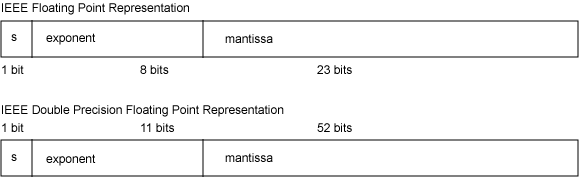
\includegraphics[width=0.7\textwidth]{float_representation}
\end{figure}

From left to right we find:
\begin{itemize}
    \item[-] the \textbf{sign} ($s$): 1 bit, $0 \rightarrow +$, $1 \rightarrow -$
    \item[-] the \textbf{exponent} ($e$): 8 or 11 bits
    \item[-] the \textbf{significand} or \textbf{mantissa} ($m$): 23 or 52 bits
\end{itemize}

The exponent does not have a sign and an exponent bias $b$ is subtracted from it (127 or 1023) in order to represent both negative and positive exponents, allowing for very large and very small numbers.
An implicit leading bit of 1 is assumed for the significand, unless the exponent is 0. In short, Python basically represents numbers like this:
\begin{equation}
  x = (-1)^s \times m \times 2^{e - b}
\end{equation}
However, Python cannot represent every number \textit{precisely}, since not every value can be decomposed into this form. This slight inevitable error is the reason why in the first example \texttt{0.1 + 0.2 == 0.3} returns \texttt{False}. 

In the following example \footnote{Source: \url{https://babbage.cs.qc.cuny.edu/IEEE-754/index.xhtml}} we take a floating-point number with an exact binary representation:
\begin{equation*}
  0.75_{10} = 0.11_{2} = 0 \times 2 + 1 \times 2^{-1} + 1 \times 2^{-2} =
  \frac{1}{2} + \frac{1}{4} = 1.5 \times 2^{-1}
\end{equation*}

\begin{verbatim}
0.75 -> 0x3F400000 = 0b|0|01111110|10000000000000000000000
sign = 0b0 = 0 -> +
exponent = 0b01111110 = 126 -> 126 - 127 = -1
significand = 0b(1)10000000000000000000000 = 12582912 -> 0b1.1 = 1.5
\end{verbatim}

The representation of any floating point number is equivalent to the ratio of two integers, where the denominator is a power of 2.
\begin{equation*}
  x = \frac{m}{2^{23 - e}} = \frac{12582912}{2^{24}} = \frac{3}{4} = 0.75
\end{equation*}

Here's an example in Python:

\input{pygments/float}

\texttt{as\_integer\_ratio()} returns the internal representation of a float. Mind this is not guaranteed to be the closest rational approximation.

Some of the most useful properties of the floating point representation in the IEEE 754 standard are:
\begin{itemize}
    \item[-] numbers at wildly different magnitudes can be easily represented;
    \item[-] the representations have the same relative accuracy at all magnitudes;
    \item[-] it allows calculations across magnitudes.
\end{itemize}
The maximum and minimum positive magnitudes are dictated by the number $n_e$ of bits in the exponent, and can be approximated as $N_{\max} \approx 2^{2^{n_e - 1}}$ and $N_{\min} \approx 2^{-2^{n_e - 1}}$. The \textbf{dynamic range} is defined as the ratio between these two limits ($N_{\max} / N_{\min}$), resulting in approximately $2^{2^{n_e}}$. The \textbf{precision} (which determines the number of exact significant digits) is dictated by the number $n_s$ of bits in the significand, yielding approximately $\log_{10}(2^{n_s + 1})$ significant decimal digits.

\bigskip

\begin{center}
\begin{tabular}{llllll}
  \hline
  Precision & Bits & $N_{\min}$ & $N_{\max}$ & Dyn. Range & Digits \\
  \hline
  \hline
  Single & $1 + 8 + 23 = 32$ & $\approx 2^{-128} \ (10^{-38})$ & $\approx 2^{128} \ (10^{38})$ & $\approx 2^{256} \ (10^{76})$ & 7 \\
  Double & $1 + 11 + 52 = 64$ & $\approx 2^{-1024} \ (10^{-308})$ & $\approx 2^{1024} \ (10^{308})$ & $\approx 2^{2048} \ (10^{616})$ & 15 \\
  \hline
\end{tabular}
\end{center}

\subsection{References}
\begin{itemize}
    \item[-] \url{https://scipy-lectures.org/}
    \item[-] \url{https://docs.quantifiedcode.com/python-anti-patterns/}
    \item[-] \url{https://sebastianraschka.com/Articles/2014_python_2_3_key_diff.html}
    \item[-] \url{https://www.python.org/dev/peps/pep-0020/}
    \item[-] \url{https://www.python.org/dev/peps/pep-0008/}
    \item[-] \url{https://docs.python-guide.org/writing/style/}
    \item[-] \url{https://docs.python.org/3/library/stdtypes.html}
    \item[-] \url{https://docs.python.org/3/tutorial/controlflow.html\#defining-functions}
    \item[-] \url{https://docs.python.org/3/tutorial/floatingpoint.html}
    \item[-] \url{https://floating-point-gui.de/}
    \item[-] \url{https://www.itu.dk/~sestoft/bachelor/IEEE754_article.pdf}
\end{itemize}
\section{Python Basics (2/2)}

\subsection{The Python standard library}

The Python ecosystem is structured into a three-level hierarchy:
\begin{itemize}
    \item[-] \textbf{Python core language} (includes all the built-in functions and types available immediately upon starting the interpreter);
    \item[-] \textbf{Python Standard Library} (provides a vast array of modules, such as math or os, that come pre-installed but must be explicitly imported);
    \item[-] \textbf{Third-party packages} (e.g. numpy, pandas) which can be installed via package managers to extend Python's capabilities for specialized tasks.
\end{itemize}
The standard library is included in every Python distribution and it is (slowly) evolving over time. With third-party packages you are on your own, although Anaconda solves many of the issues. If you are using GNU-Linux your package manager is probably taking care of everything for you. Of course you can write your own modules, too.

Anything that is outside the core is loaded into memory via an \texttt{import} statement.

\subsubsection{The import system}
This example sums up the basics and best practices of the import system:

\begin{verbatim}
from math import *
[...]
# Terrible: where the hell is sqrt coming from?
x = sqrt(2.)

from math import sqrt
[...]
# Better: if you haven't redefined sqrt this is from the math library
x = sqrt(2.)

import math
[...]
# Best: five more characters, but at least it is clear where sqrt is coming from
x = math.sqrt(2.)
\end{verbatim}

The \texttt{\$PYTHONPATH} environment variable is your friend to control where you want to import modules from (you will need to tweak it when you start writing your own packages). You will need suitable \texttt{\_\_init\_\_.py} files to navigate directories (see \url{https://lucabaldini.github.io/metarep/setup.html}).

The import system is fairly flexible, so take advantage of it but don't abuse it. For example, this is ok\ldots

\medskip
\input{pygments/import1}

\ldots but this is a catastrophe.

\medskip
\input{pygments/import2}

\subsection{Brief overview of the standard library}
\subsubsection{- \texttt{time}, \texttt{datetime} and \texttt{calendar}}

The modules \texttt{time}, \texttt{datetime} and \texttt{calendar} are a collection of facilities related to date and time that can be used to measure the execution time of your scripts, convert from time to date and vice-versa and so on. This is anything but trivial. Ever heard of UNIX time? And UTC? And time zones?

\subsubsection{- \texttt{math}}
\begin{verbatim}
Python 3.7.4 (default, Jul  9 2019, 16:32:37)
[GCC 9.1.1 20190503 (Red Hat 9.1.1-1)] on linux
Type "help", "copyright", "credits" or "license" for more information.
>>> import math
>>> dir(math)
['__doc__', '__file__', '__loader__', '__name__', '__package__', '__spec__',
'acos', 'acosh', 'asin', 'asinh', 'atan', 'atan2', 'atanh', 'ceil', 'copysign',
'cos', 'cosh', 'degrees', 'e', 'erf', 'erfc', 'exp', 'expm1', 'fabs',
'factorial', 'floor', 'fmod', 'frexp', 'fsum', 'gamma', 'gcd', 'hypot', 'inf',
'isclose', 'isfinite', 'isinf', 'isnan', 'ldexp', 'lgamma', 'log', 'log10',
'log1p', 'log2', 'modf', 'nan', 'pi', 'pow', 'radians', 'remainder', 'sin',
'sinh', 'sqrt', 'tan', 'tanh', 'tau', 'trunc']
>>>
\end{verbatim}

\medskip

Note: If you work a lot with arrays you will end up using mostly \texttt{numpy}.

\subsubsection{- \texttt{random}}
\begin{verbatim}
Python 3.7.4 (default, Jul  9 2019, 16:32:37)
[GCC 9.1.1 20190503 (Red Hat 9.1.1-1)] on linux
Type "help", "copyright", "credits" or "license" for more information.
>>> import random
>>> print(dir(random))
['BPF', 'LOG4', 'NV_MAGICCONST', 'RECIP_BPF', 'Random', 'SG_MAGICCONST',
'SystemRandom', 'TWOPI', '_BuiltinMethodType', '_MethodType', '_Sequence',
'_Set', '__all__', '__builtins__', '__cached__', '__doc__', '__file__',
'__loader__', '__name__', '__package__', '__spec__', '_acos', '_bisect', '_ceil',
'_cos', '_e', '_exp', '_inst', '_itertools', '_log', '_os', '_pi', '_random',
'_sha512', '_sin', '_sqrt', '_test', '_test_generator', '_urandom', '_warn',
'betavariate', 'choice', 'choices', 'expovariate', 'gammavariate', 'gauss',
'getrandbits', 'getstate', 'lognormvariate', 'normalvariate', 'paretovariate',
'randint', 'random', 'randrange', 'sample', 'seed', 'setstate', 'shuffle',
'triangular', 'uniform', 'vonmisesvariate', 'weibullvariate']
>>>
\end{verbatim}

\medskip

\subsubsection{- \texttt{os}, \texttt{os.path}, \texttt{glob}, \texttt{shutil} and \texttt{pathlib}}
The modules \texttt{os}, \texttt{os.path}, \texttt{glob}, \texttt{shutil} and \texttt{pathlib} let you interact with the underlying operating system. You can for example access the filesystem (access, create and copy files and directories), list directory content, access environment variables, absolute and relative paths and execute OS commands. All of this in a \textit{cross-platform} fashion.

\subsubsection{- \texttt{argparse}}
\texttt{argparse} is a parser for command-line options. What does this mean?
Ever found yourself modifying the source code and running your program with different parameters? This is a terrible practice and git will complain about modified files. Instead, you can do something like this:

\begin{Verbatim}[label=\makebox{\url{argparse_example.py}},commandchars=\\\{\}]
\PY{k}{import} \PY{n+nn}{argparse}

\PY{n}{parser} \PY{o}{=} \PY{n}{argparse}\PY{o}{.}\PY{n}{ArgumentParser}\PY{p}{(}\PY{p}{)}
\PY{n}{parser}\PY{o}{.}\PY{n}{add\PYZus{}argument}\PY{p}{(}\PY{l+s+s2}{\PYZdq{}}\PY{l+s+s2}{\PYZhy{}\PYZhy{}speed}\PY{l+s+s2}{\PYZdq{}}\PY{p}{,} \PY{n}{type}\PY{o}{=}\PY{n+nb}{int}\PY{p}{,} \PY{n}{default}\PY{o}{=}\PY{l+m+mi}{5}\PY{p}{)}

\PY{n}{args} \PY{o}{=} \PY{n}{parser}\PY{o}{.}\PY{n}{parse\PYZus{}args}\PY{p}{(}\PY{p}{)}
\PY{n+nb}{print}\PY{p}{(}\PY{l+s+sf}{f}\PY{l+s+s2}{\PYZdq{}}\PY{l+s+s2}{I}\PY{l+s+s2}{\PYZsq{}}\PY{l+s+s2}{m running at this speed: }\PY{l+s+si}{\PYZob{}}\PY{n}{args}\PY{o}{.}\PY{n}{speed}\PY{l+s+si}{\PYZcb{}}\PY{l+s+s2}{\PYZdq{}}\PY{p}{)}

[Output]
PS C:\PYZbs{}Università\PYZbs{}Magistrale\PYZbs{}Computing Methods> python script.py --speed 10
I'm running at this speed: 10
PS C:\PYZbs{}Università\PYZbs{}Magistrale\PYZbs{}Computing Methods> python script.py --speed 15
I'm running at this speed: 15
\end{Verbatim}

\subsubsection{- \texttt{logging}}
Ever found yourself inserting debug \texttt{print()} statements in the code when needed? This is another terrible practice and git will complain about modified files. Imagine if there was a thing that allowed you to label messages with different levels of severity (e.g. debug, info, warning, error) and dynamically set a global filter on the severity level (e.g. do not print debug messages). This thing exists and is called \texttt{logging}. \textbf{Always prefer \texttt{logging} over \texttt{print}}. Here's an example:

\begin{Verbatim}[label=\makebox{\url{logging_config.py}},commandchars=\\\{\}]
\PY{k}{import} \PY{n+nn}{logging}

\PY{c+c1}{\PYZsh{} 1. Configure the logging settings}
\PY{n}{logging}\PY{o}{.}\PY{n}{basicConfig}\PY{p}{(}
    \PY{n}{level}\PY{o}{=}\PY{n}{logging}\PY{o}{.}\PY{n}{INFO}\PY{p}{,}
    \PY{n}{format}\PY{o}{=}\PY{l+s+s1}{\PYZsq{}}\PY{l+s+s1}{\PYZpc{}(asctime)s - \PYZpc{}(levelname)s - \PYZpc{}(message)s}\PY{l+s+s1}{\PYZsq{}}\PY{p}{,}
    \PY{n}{handlers}\PY{o}{=}\PY{p}{[}
        \PY{n}{logging}\PY{o}{.}\PY{n}{FileHandler}\PY{p}{(}\PY{l+s+s2}{\PYZdq{}}\PY{l+s+s2}{program\PYZus{}logs.log}\PY{l+s+s2}{\PYZdq{}}\PY{p}{)}\PY{p}{,} \PY{c+c1}{\PYZsh{} Saves to a file}
        \PY{n}{logging}\PY{o}{.}\PY{n}{StreamHandler}\PY{p}{(}\PY{p}{)}                 \PY{c+c1}{\PYZsh{} Prints to terminal}
    \PY{p}{]}
\PY{p}{)}

\PY{k}{def} \PY{n+nf}{divide}\PY{p}{(}\PY{n}{a}\PY{p}{,} \PY{n}{b}\PY{p}{)}\PY{p}{:}
    \PY{n}{logging}\PY{o}{.}\PY{n}{info}\PY{p}{(}\PY{l+s+sf}{f}\PY{l+s+s2}{\PYZdq{}}\PY{l+s+s2}{Attempting to divide }\PY{l+s+si}{\PYZob{}}\PY{n}{a}\PY{l+s+si}{\PYZcb{}}\PY{l+s+s2}{ by }\PY{l+s+si}{\PYZob{}}\PY{n}{b}\PY{l+s+si}{\PYZcb{}}\PY{l+s+s2}{\PYZdq{}}\PY{p}{)}
    \PY{k}{try}\PY{p}{:}
        \PY{n}{result} \PY{o}{=} \PY{n}{a} \PY{o}{/} \PY{n}{b}
        \PY{n}{logging}\PY{o}{.}\PY{n}{info}\PY{p}{(}\PY{l+s+s2}{\PYZdq{}}\PY{l+s+s2}{Division successful}\PY{l+s+s2}{\PYZdq{}}\PY{p}{)}
        \PY{k}{return} \PY{n}{result}
    \PY{k}{except} \PY{n+ne}{ZeroDivisionError}\PY{p}{:}
        \PY{n}{logging}\PY{o}{.}\PY{n}{error}\PY{p}{(}\PY{l+s+s2}{\PYZdq{}}\PY{l+s+s2}{Attempted to divide by zero!}\PY{l+s+s2}{\PYZdq{}}\PY{p}{)}
        \PY{k}{return} \PY{k+kc}{None}

\PY{c+c1}{\PYZsh{} Test the logger}
\PY{n}{divide}\PY{p}{(}\PY{l+m+mi}{10}\PY{p}{,} \PY{l+m+mi}{2}\PY{p}{)}
\PY{n}{divide}\PY{p}{(}\PY{l+m+mi}{10}\PY{p}{,} \PY{l+m+mi}{0}\PY{p}{)}

[Output]
/Università/Magistrale/Computing Methods/script.py"
2026-01-30 11:40:02,178 - INFO - Attempting to divide 10 by 2
2026-01-30 11:40:02,178 - INFO - Division successful
2026-01-30 11:40:02,178 - INFO - Attempting to divide 10 by 0
2026-01-30 11:40:02,178 - ERROR - Attempted to divide by zero!
\end{Verbatim}

\texttt{loguru} is another third-party package that can be useful for the same purpose. 

\subsection{References}
\begin{itemize}
    \item[-] \url{https://docs.python.org/3/library/}
    \item[-] \url{https://pypi.org/}
    \item[-] \url{https://docs.python.org/3/reference/import.html}
    \item[-] \url{https://docs.python-guide.org/}
    \item[-] \url{https://docs.quantifiedcode.com/python-anti-patterns/}
\end{itemize}
\section{Algorithms and data structures}

\subsection{What is an algorithm?}
An \textbf{algorithm} is a sequence of instructions to perform a computation. 
Algorithms can be expressed in several different ways such as flowcharts, pseudo-code, and working code snippets. The sequence of operations must be expressed unambiguously. Using the right algorithm sometimes makes all the difference between being able to attack a problem in a practical time or not.

\subsubsection{Example: sequential vs. binary search}
Let's consider a classic problem: finding an element in a sorted list. Let's try and solve it in the two most intuitive ways.

The first method is the sequential search which utilizes a bit of brute force: you loop over the list until you find (or do not find) the target.
    
The second method is the Binary search, schematically represented below:
\begin{itemize}
    \item[-] Start from the middle (if that's the target you're done)
    \item[-] If the target is smaller (larger) than the element in the center, bisect the half-list on the left (right)
    \item[-] Iterate until you've found the target (or exhausted the list)
\end{itemize}
\begin{center}
    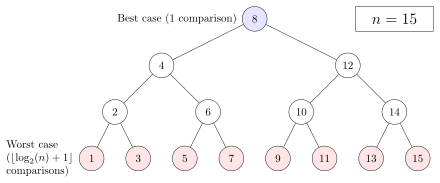
\includegraphics[width=0.6\textwidth]{binary_search}
\end{center}
As an exercise, try to determine which algorithm is more efficient. if you think about it, this problem is essentially similar to that of finding a person in the phone book.

\subsection{Complexity of an algorithm}

As an example, let's try to find the largest element in a list of length $n$ implementing this problem in Python:

\input{pygments/find_max}

How many fundamental instructions does this code execute? You should realize that this is an ill-posed question, since the answer depends on the structure of the list. Nonetheless, let's count:
\begin{itemize}
    \item[-] One assignment and one list lookup at the beginning: $2$
    \item[-] One lookup, one assignment and one comparison for each iteration in the for loop: $3(n - 1)$
    \item[-] A variable number of assignments: between $0$ and $(n - 1)$
    \item[-] One final return instruction: 1
\end{itemize}
Answer: anything between $3n$ and $4n - 1$, depending on the input list.

What does this example tell us?

\underline{Message \#1:} \textit{The exact number of fundamental instructions that an algorithm performs is not determined a priori}. It depends on the input data, instead, and so does the running time.

There are a few questions that you can legitimately ask, anyway:
\begin{itemize}
    \item[-] How many instructions in the \textit{worst case}?
    \item[-] How many instructions in the \textit{best case}?
    \item[-] How many instructions on \textit{average}?
\end{itemize}

\underline{Message \#2:} \textit{The exact number of operations doesn't really matter}, does it? Different machines have different executions speeds and different languages have different meanings of \textit{fundamental instruction}.

\underline{Message \#3:} Still, \textit{the running time is related to the number of fundamental instructions}.

With these messages in mind, how can we define how "fast" an algorithm is? The easiest way is to analyze its asymptotic behavior.

\subsubsection{Asymptotic behavior and big-O notation}

Say you have an algorithm operating on an input of length $n$ (e.g., a list with $n$ elements or a string with $n$ characters).
How many fundamental instructions $N$ does it take for your algorithm to run? \footnote{As said before, this question is ambiguous. The correct one should be "How many fundamental instructions $N$ does it take for your algorithm to run \textit{in the worst case}?" (easiest to compute) or "\textit{in the average case}?".} When asking this question, you are trying to find a function $f$ such that:
\begin{equation*}
    N = f(n)    
\end{equation*}
Since the real problems in algorithm implementation come around when $n$ is really high, we are interested in the \textbf{asymptotic behaviour} of f: drop all the terms that grow slowly with $n$ and only keep the one that grows faster:
\begin{equation*}
    4n - 1 \approx 4n \quad\text{and}\quad 2n^2 + 6n + 3 \approx 2n^2 \quad \text{for} \quad n \xrightarrow{} +\infty
\end{equation*}
Let's go one step further, and say that we neglect the multiplicative factor in front of the leading term:
\begin{equation*}
    4n - 1 \approx n \quad\text{and}\quad 2n^2 + 6n + 3 \approx n^2    
\end{equation*}
That's the so-called \textbf{big-O notation}: the two algorithms in the example are $O(n)$ (the less complex one) and $O(n^2)$ (the more complex one). Your goal should be to write an algorithm with the lowest possible complexity. Take a look at the graph below: if $n = 10^6$ and you can beat down the complexity from $n^2$ to $n\log(n)$ you are cutting down the execution time by one million.

\begin{center}
    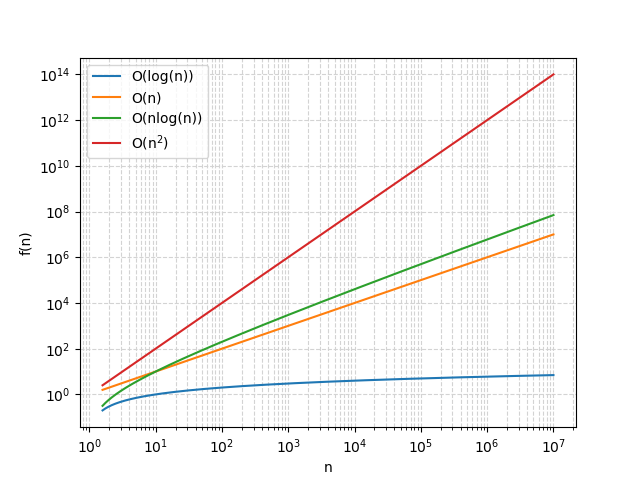
\includegraphics[width=0.5\textwidth]{bigo}
\end{center}

Now, how can you measure the asymptotic behaviour of an algorithm?
\begin{itemize}
    \item[-] By brute force: implement the algorithm, run it on input data of different sizes and time the run (be careful: results may vary from run to run) and plot the running time vs. input size.
    \item[-] By analysis: count the instructions and evaluate the best, worst and average case (this can be difficult for complex programs, and subject to the idiosyncrasies of the language).
    \item[-] "By eye" (e.g. one loop: $O(n)$; two sequential loops: $O(n)$; two nested loops: $O(n^2)$)
\end{itemize}
Here's a fun article about the complexity of songs: \url{http://www.cs.bme.hu/~friedl/alg/knuth_song_complexity.pdf}

\subsection{Data structures}
During this course you will have to work on real-life data. In which "objects" can data be stored? How fast can you operate on such objects ($\equiv$ how complex are the algorithms that let you interact with such data)? Here are two examples of \textbf{data structures} that you should master while coding in Python: lists and hash tables (dictionaries).

\subsubsection{Lists}

The following table summarizes the time complexity of common operations on Python lists:

\begin{center}
\begin{tabular}{lll}
    \hline
    Operation & Average case & Worst case\\
    \hline
    \hline
    Copy & O(n) & O(n)\\
    Append & O(1) & O(1)\\
    Insert & O(n) & O(n)\\
    Get Item & O(1) & O(1)\\
    Set Item & O(1) & O(1)\\
    Delete Item & O(n) & O(n)\\
    Iteration & O(n) & O(n)\\
    min(s), max(s) & O(n) & \\
    Get Length & O(1) & O(1)\\
    \hline
\end{tabular}
\end{center}

 Do you remember how to index a list? You should, but here is a simple figure:
 
\begin{center}
    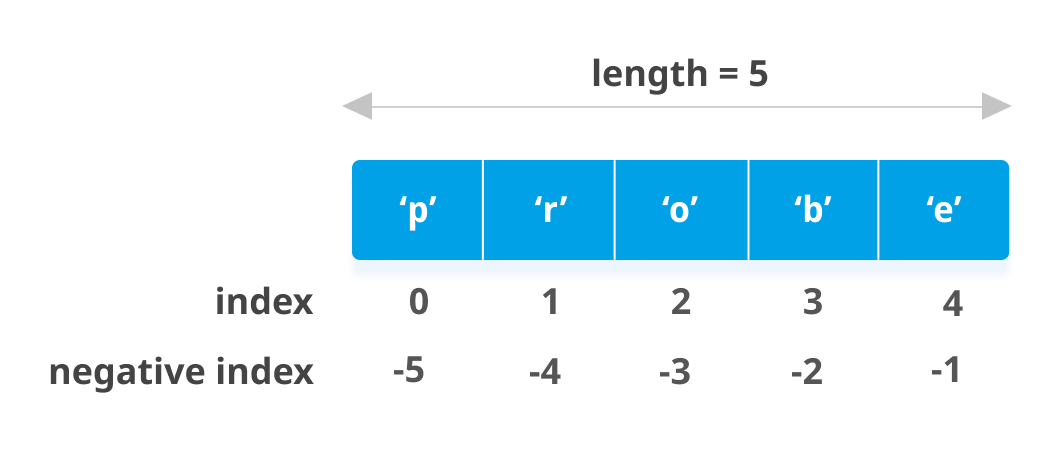
\includegraphics[width=0.5\textwidth]{python-list}
\end{center}

\subsubsection{Hash tables}
A \textbf{hash table} is a data structure that implements an associative array, a structure that can map keys to values. It is designed to optimize data retrieval, allowing for extremely fast access to data regardless of the size of the dataset.

\begin{center}
    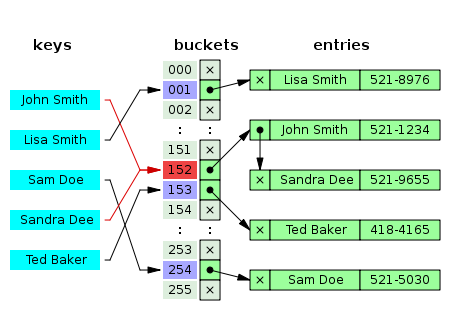
\includegraphics[width=0.5\textwidth]{hash_table}
\end{center}

The efficiency of a hash table relies on a hashing function. When you insert a key-value pair (e.g., \texttt{\{'name': 'Alice'\}}), the system performs the following steps:
\begin{enumerate}
    \item[-] Hashing: The key ('name') is passed through a hash function, which converts it into a unique integer (the hash).
    \item[-] Indexing: This integer is used to calculate an index (usually via the modulo operator) corresponding to a specific slot, or bucket, in an array.
    \item[-] Storage: The value ('Alice') is stored in that specific bucket.
\end{enumerate}

When you want to retrieve the value, the system re-calculates the hash of the key, finds the index, and instantly retrieves the value without searching through the entire list.

Why do I even bring this up? Because Python dictionaries are highly optimized hash tables. The performance of dictionary operations is summarized in the following table:

%\begin{center}
%    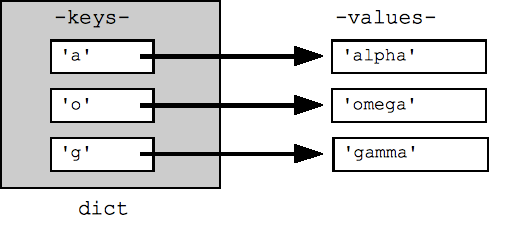
\includegraphics[width=0.5\textwidth]{python-dict}
%\end{center}

\begin{center}
\begin{tabular}{lll}
    \hline
    Operation & Average case & Worst case\\
    \hline
    \hline
    Copy & O(n) & O(n)\\
    Get Item & O(1) & O(n)\\
    Set Item & O(1) & O(n)\\
    Delete Item & O(1) & O(n)\\
    Iteration & O(n) & O(n)\\
    \hline
\end{tabular}
\end{center}

Since the array size is finite and the set of possible keys is infinite, a \textbf{collision} occurs when two distinct keys result in the same index. Python can solve this problem thanks to a method called \textit{open addressing} (for more info about open addressing visit \url{https://adamgold.github.io/posts/python-hash-tables-under-the-hood/}).

Note that when a float corresponds to an integer, its hash is the same as that of the integer. The hash is used to map keys into indices, therefore $3$ and $3.$ are the same key to a dictionary. For example:

\input{pygments/dict_hashing}

\bigskip

\subsection{A real-life example: sorting}

Let's consider a naive implementation of a sorting algorithm:

\input{pygments/sloppy_sort}

Say you are asked to implement an algorithm to sort a list. Chances are that you would come up with two nested loops, O($n^2$). However, there is already a rich variety of sorting algorithms on the market, so you should focus on mastering them instead of creating one of your own.

The following table summarizes the time and space complexity of several popular sorting algorithms:

\begin{center}
    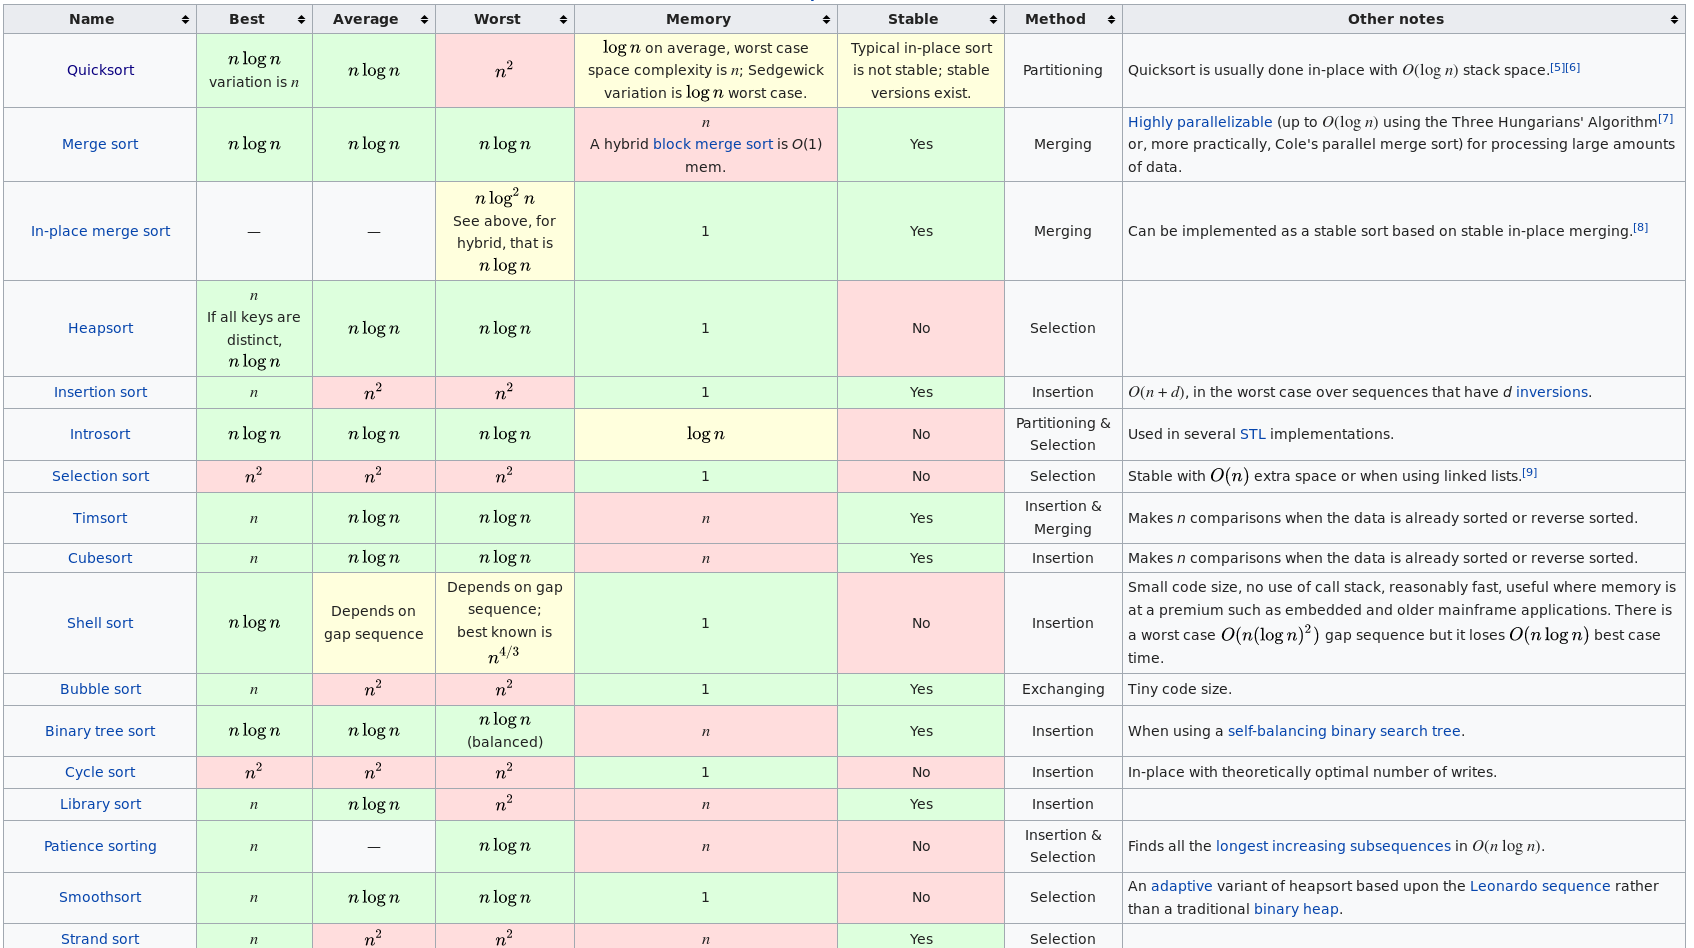
\includegraphics[width=\textwidth]{sorting_algs}
\end{center}

The \texttt{.sort()} method for lists in Python uses a hybrid algorithm derived from merge sort and insertion sort called \textbf{timsort} \footnote{The name comes from Tim Peters.}. It works by finding subsequences of the data that are already ordered and using that knowledge to sort the remainder more efficiently (\textit{"Although practicality beats purity"}, The Zen of Python).

Here is a quick example of how to use the built-in sorting method in Python:

\input{pygments/timsort}

\subsection{References}
\begin{itemize}
    \item[-] \url{https://en.wikipedia.org/wiki/Algorithm}
    \item[-] \url{https://discrete.gr/complexity/}
    \item[-] \url{https://wiki.python.org/moin/TimeComplexity}
    \item[-] \url{https://en.wikipedia.org/wiki/Sorting_algorithm}
    \item[-] \url{https://bugs.python.org/file4451/timsort.txt}
    \item[-] \url{https://en.wikipedia.org/wiki/Timsort}
\end{itemize}
\section{OOP introduction: Basics, inheritance and composition}

\subsection{Smart variables}
Working with containers like lists or dictionaries, you may have noticed that they can do many things besides holding the data. You can extend a list using \texttt{append()} or \texttt{insert()}. Trying to access a non-existent index in a list triggers a specific error (\texttt{IndexError}). You can iterate on a list using the handy for-loop Python syntax and so on. In other words, a list is a variable that, in addition to its data, shows some kind of specific \textit{behaviour}. How is that implemented?

\subsection{Object Oriented Programming (OOP)}
The so-called \textbf{Object Oriented Programming (OOP)} is a programming paradigm based on \textit{objects}. An \textbf{object} is a code entity that has:
\begin{itemize}
    \item[-] a \textbf{state} $\rightarrow$ data (usually called \textbf{member variables} or \textbf{attributes})
    \item[-] a \textbf{behaviour} $\rightarrow$ functions (usually called \textbf{member functions} or \textbf{methods})
\end{itemize}

The idea is this: \textit{keep together the variables and the code that manipulates them}. 

As the name suggests, OOP is often adopted for modelling systems that are naturally described in terms of objects such as:
\begin{itemize}
    \item[-] Physical simulations: Geant4 (C++), SimPy (Python) \ldots
    \item[-] Graphics engines and game development: Unity (C\#), Unreal Engine (C++) \ldots
    \item[-] Graphical User Interfaces (GUI): Qt / PySide (C++/Python), JavaFX (Java), .NET WinForms (C\#) \ldots
\end{itemize}
OOP is also used in enterprise applications, web frameworks, compilers, OS, robotics, embedded systems and so on.

Object-oriented programming is one of the most widely used paradigms today. That does not necessarily mean it is the best one, nor the right tool for any job \footnote{See \url{https://en.wikipedia.org/wiki/Object-oriented_programming\#Criticism}}. There are a number of famous programmers who really dislike it (e.g. Linus Torvalds himself). Still, it is something you definitely want in your toolbox since there is a fairly good chance that you will have to interact with some OOP code in your life. Also, every popular language nowadays is object-oriented (look for example at the following figure from \url{https://www.tiobe.com/tiobe-index/}).

\begin{center}
    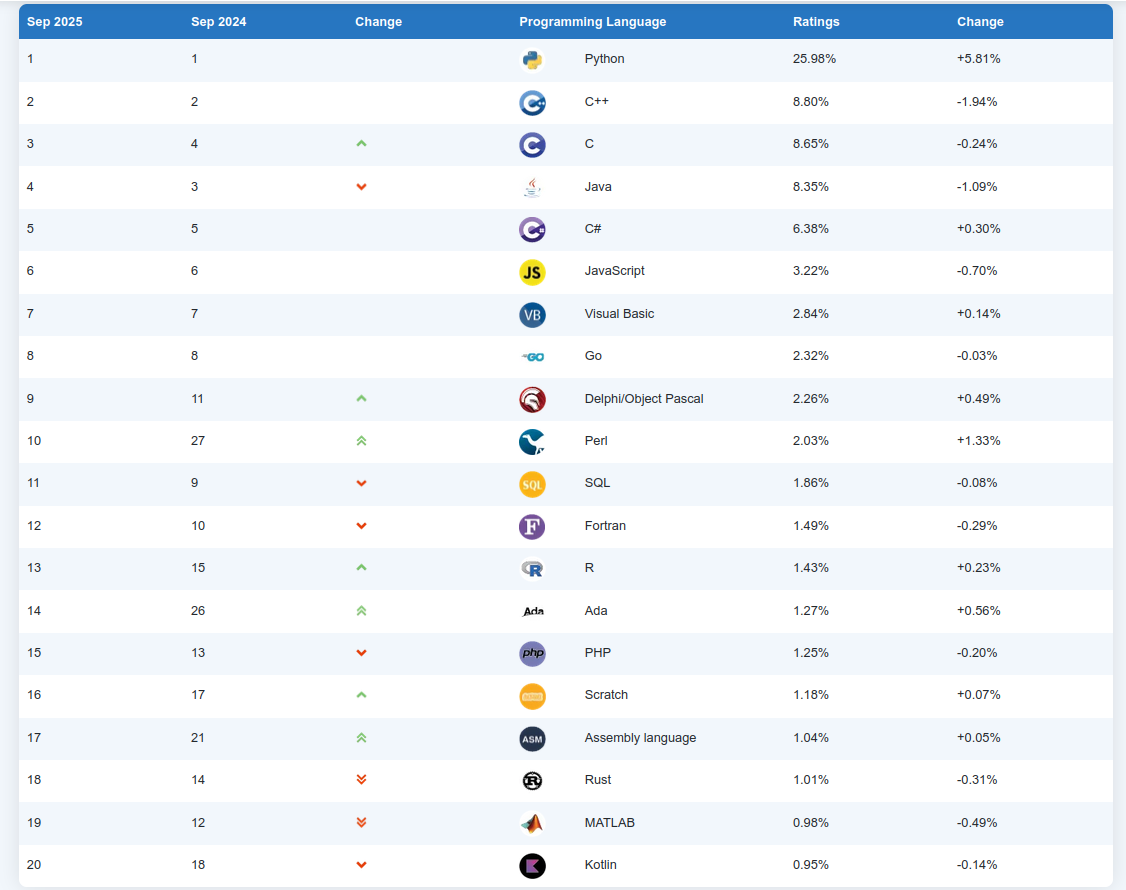
\includegraphics[width=0.55\textwidth]{tiobe2025.png}
\end{center}


\subsection{OOP: classes and objects in practice}
Here are the two most fundamental definitions for OOP:
\begin{itemize}
    \item[-] A \textbf{class} is a blueprint for creating objects.
    \item[-] An \textbf{object} is a concrete realization of a class.
\end{itemize}

You can imagine a class like a project, which is used to describe how objects are built and how they work. You can have multiple objects of the same class.

The relationship is similar to the one between types and variables: a type is an abstract concept, describing how a variable is represented in memory. A variable is a concrete realization of it. You can have several variables of the same type (like several integers or several strings).
Indeed, to some extent, a class is the generalization of the concept of type. It specifies not only how an object \textit{is made} but also how \textit{it behaves}.

\begin{center}
    
\includegraphics[width=0.2\textwidth]{television.png}
\end{center}

\medskip

Let's consider a familiar object, like a television. 

It has a \textit{state}. Is it on or off (and possibly in standby)? What is the currently displayed channel? What is its volume, brightness, contrast, etc\ldots?

It also has a \textit{behaviour}: pressing the `power' button will turn it ON/OFF, rotating the volume knob will increase/decrease the volume, using the buttons on the remote control will change the displayed channel, brightness, contrast etc\dots. 

How would that be represented in the code? The state can be represented by some \textbf{attributes} (variables). For example, a boolean can represent the ON/OFF state. For the currently displayed channel you can use an integer. Volume, contrast, luminosity etc\dots will all get their own variable(s).

The behaviour can be implemented through the \textbf{methods}. For example the \texttt{turn\_on()} and \texttt{turn\_off()} functions may change the value of the variable and also produce all the related changes (i.e. start/stop video and audio). You will probably have the \texttt{next\_channel()} and \texttt{previous\_channel()} functions for zapping and so on. Of course it can be much more complex than that.

Attributes and methods are collectively called \textbf{members} of the class. Each object of a specific class is an \textbf{instance} of that class. The \texttt{type()} built-in function will tell you which class its argument is an instance of. 

With all that in mind, let's create the \texttt{Television} class:

\input{pygments/class_tv_basic}

\hrulefill

It is important to know that OOP is the base of Python and that means that in Python everything is an object of some class. Look at this example:
\input{pygments/everything_is_a_class}

\hrulefill

As previously described, let's add some methods to our \texttt{Television} class so it can actually do something. Always remember that a class method must always have \textbf{\texttt{self}} as its first positional argument.

\input{pygments/class_methods}

Attributes are typically added via the class \textbf{constructor}. The constructor is a special method that is called automatically each time a class instance is created. A specificity of the constructor is that it cannot return anything. In Python the constructor is the \textbf{\texttt{\_\_init\_\_}} method\footnote{Actually the real constructor - the function responsible for creating the class instances - is the \texttt{\_\_new\_\_} operator, but 99\% of the time you don't need to define that, as all classes have a default one which does the job for you.}. Class methods like \texttt{\_\_init\_\_}, with the name surrounded by two underscores, are called \textbf{special} methods or \textbf{dunder} methods. \textbf{Good practice: always define all your class attributes inside the constructor}. Note how, while writing your class, you must access its members using the \texttt{self.} prefix.

\input{pygments/class_constructor}

\subsection{The importance of namespaces in OOP}
\textit{"Namespaces are one honking great idea - let's do more of those!"}, The Zen of Python.

A \textbf{namespace} in Python is essentially a dictionary of \emph{unique} names, each one associated with an object (which can be anything: a variable, a function, a class etc\dots).

\begin{center}
    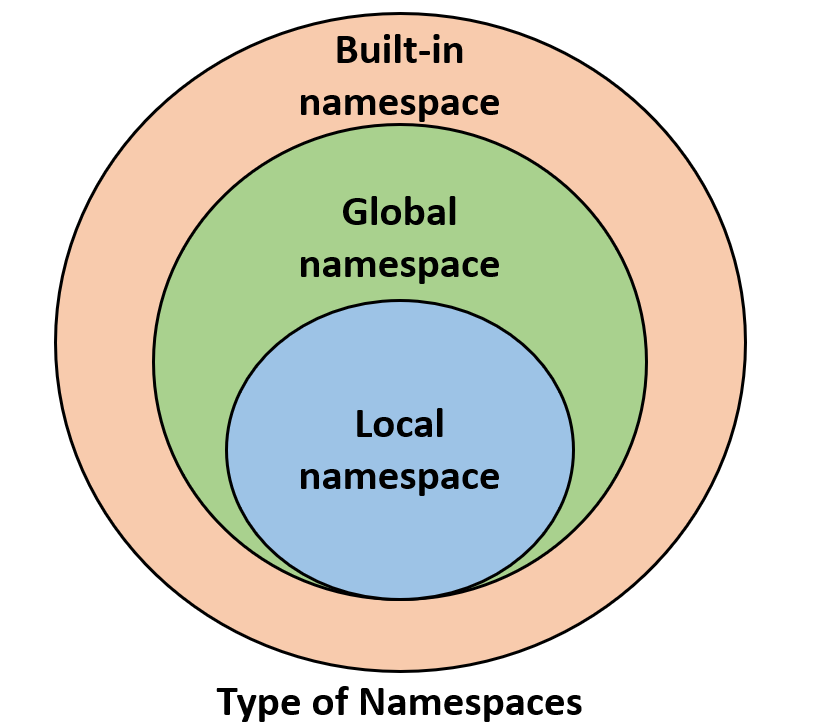
\includegraphics[width=0.4\textwidth]{types_namespace.png}
\end{center}

Python creates separate namespaces for many things: for example, each time a function is called, a namespace for local variables is created. You can access objects in the local namespace (and those above -- see picture) just with their names; for others you need the \texttt{.} (dot) operator. As the ones who are used to programming in C certainly know, the space of visibility of a variable is called its \textbf{scope}. Look at the following example.

\begin{Verbatim}[label=\makebox{\url{namespaces_example.py}},commandchars=\\\{\}]
\PY{k}{import} \PY{n+nn}{math}

\PY{c+c1}{\PYZsh{} A variable in the global namespace}
\PY{n}{global\PYZus{}var} \PY{o}{=} \PY{l+s+s2}{\PYZdq{}}\PY{l+s+s2}{I am global}\PY{l+s+s2}{\PYZdq{}}

\PY{c+c1}{\PYZsh{} Proof that namespace is a dictionary: accessing via key}
\PY{n+nb}{print}\PY{p}{(}\PY{n+nb}{globals}\PY{p}{(}\PY{p}{)}\PY{p}{[}\PY{l+s+s1}{\PYZsq{}}\PY{l+s+s1}{global\PYZus{}var}\PY{l+s+s1}{\PYZsq{}}\PY{p}{]}\PY{p}{)}

\PY{k}{def} \PY{n+nf}{my\PYZus{}function}\PY{p}{(}\PY{p}{)}\PY{p}{:}
    \PY{c+c1}{\PYZsh{} New namespace created for this function call}
    \PY{n}{local\PYZus{}var} \PY{o}{=} \PY{l+m+mi}{10}
    
    \PY{c+c1}{\PYZsh{} Accessing local (direct name) and global (scope above)}
    \PY{n+nb}{print}\PY{p}{(}\PY{l+s+sf}{f}\PY{l+s+s2}{\PYZdq{}}\PY{l+s+s2}{Local: }\PY{l+s+si}{\PYZob{}}\PY{n}{local\PYZus{}var}\PY{l+s+si}{\PYZcb{}}\PY{l+s+s2}{, Global: }\PY{l+s+si}{\PYZob{}}\PY{n}{global\PYZus{}var}\PY{l+s+si}{\PYZcb{}}\PY{l+s+s2}{\PYZdq{}}\PY{p}{)}

\PY{n}{my\PYZus{}function}\PY{p}{(}\PY{p}{)}

\PY{c+c1}{\PYZsh{} Using the dot operator to access objects in other namespaces}
\PY{n+nb}{print}\PY{p}{(}\PY{n}{math}\PY{o}{.}\PY{n}{pi}\PY{p}{)}

[Output]
I am global
Local: 10, Global: I am global
3.141592653589793
\end{Verbatim}

\subsubsection{Instance attributes vs. class attributes}
Each class has a namespace. Plus, each instance of the class gets its own additional namespace. The class namespace is automatically visible from each instance namespace, but not the opposite. An attribute in an instance namespace is an \textbf{instance attribute}, and cannot be seen or modified by other instances of the class. An attribute in the class namespace is a \textbf{class attribute} and is shared among all the instances. Since class attributes are not related to a specific instance, they can be accessed without creating one. That also means that \textit{changing a class attribute in the class namespace will change it for every instance}. Class attributes are useful to set class constants, or default values, or share data among instances. Look at the following example for clarity.

\input{pygments/class_attributes_3}

\subsubsection{Short summary 1: OOP basics}
\begin{itemize}
  \item \textbf{Object-Oriented Programming (OOP)} is a widely used paradigm, supported by most modern languages (including Python).
  \item An \textbf{object} has:
    \begin{itemize}
      \item \textbf{State} $\rightarrow$ stored in attributes (variables).
      \item \textbf{Behavior} $\rightarrow$ defined by methods (functions).
    \end{itemize}
  \item A \textbf{class} is a blueprint for creating objects; each object is an \textbf{instance} of a class.
  \item In Python:
    \begin{itemize}
      \item Define with \texttt{class} and instantiate with \texttt{()}.
      \item Access members with the dot \texttt{.} operator.
      \item Methods always take the instance as the first argument (\texttt{self}).
    \end{itemize}
  \item Define attributes inside the \textbf{constructor} (\texttt{\_\_init\_\_}).
  \item \begin{itemize}
      \item \textbf{Instance attributes} $\rightarrow$ unique to each object
      \item \textbf{Class attributes} $\rightarrow$ shared across all instances.
  \end{itemize}
\end{itemize}

\subsection{Encapsulation: hidden state and interfaces}
Look back at the TV example. Note that part of the state is hidden from the user e.g. internal switches, transistors, etc\dots You do not need to know what's going on inside the case to operate a TV. All you need to know is how to use the \textit{interface} (the remote control, the knobs, the power button, the plug\dots). The \textit{implementation} details are hidden: only the TV producer cares about them, not the user.

This leads us to the concept of \textbf{encapsulation}: \textit{the state of an object should only be accessed and altered through its publicly exposed interface}. That way it is easier to find bugs: you know that, if something is wrong with an object, the problem lies inside the class code. That way you can also \textit{enforce behaviour}: for example you can prevent the user from changing the channel if the TV is off, as in the following example:

\input{pygments/class_tv_zapping}

At this point you may be wondering: "I can read and modify any class attribute from outside the class using the \texttt{.} (dot) operator. Doesn't that break encapsulation?". Yes, it does, but there are ways to fix it.

In languages like C++ you can explicitly declare that some class attributes (and methods) are \textit{private}. In Python there is no concept of \textit{enforced} private attributes. However, there exists a convention that \textit{any attribute/method name prepended by one or two underscore(s) should be considered "private"}. It's like a warning for the class user: you should never access that directly. In the case of two underscores Python will actually do a subtle thing to help keep the data private: it will prepend \texttt{\_classname} to the actual attribute name (see next example). However, not everyone in the Python community loves that. "Never, ever use two leading underscores. This is annoyingly private!" (cit. Ian Bicking, creator of pip, virtualenv, and many others).

\input{pygments/class_tv_private}

The possibility of making variables "private" (enforced or not) is not enough of course, because sometimes we still want to let the user read or even modify the value of the attribute. The "old" solution for that is providing access functions (the infamous getters/setters), but the awesome solution is using \textbf{properties} (since Python 2.2). Properties look similar to getters and setters, but with a twist: you keep accessing the attribute with the dot operator. In order to understand why this makes a \textit{huge} difference, let's start with an example: suppose you have a class for 2D vectors:

\input{pygments/vector2d_xy}

Suppose you later realize that you use your \texttt{Vector2d} a lot for performing rotations. It would be much faster to store the angle and the module, instead of x and y, as the rotation would reduce to a simple addition of the angles. You may think of rewriting your class in this way:

\input{pygments/vector2d_rtheta}

Now, however, you have a big problem: your old code is broken. In every place where your were calling \texttt{v.x} or \texttt{v.module()} now you get an error that needs to be fixed. If other people use your code that is even worse, because you are breaking \textit{their} code. Without properties the solution would have been to design the class from the start with private attributes and access functions.

Here is an example of how encapsulation was enforced in older versions of Python to solve this problem. \underline{You should never do this.}
\input{pygments/vector2d_old_enc}

The class data are now "encapsulated", but that is still not ideal:
\begin{enumerate}
    \item You have written a lot of code just to provide access to a bunch of variables.
    \item You will have to write even more methods if you want to let the user modify those variables as well (e.g. \texttt{set\_x()}, \texttt{set\_y()} and so on).
    \item You have to write all this code right from the start, even if you never need it, otherwise you run the risk of getting screwed later.
\end{enumerate}
\textbf{Properties} solve the problem by \textit{emulating attributes}. In Python they are implemented using the \texttt{@property} decorator just like this:

\input{pygments/vector2d_property}

To modify the value of the property, you now need a \textbf{property setter}, which is a function that must have the same name as the property and is identified by the decorator \texttt{@property\_name.setter}. In our example, whenever you modify \texttt{v.module} or \texttt{v.angle} you also update the value of \texttt{v.x}:

\input{pygments/vector2d_property_setter}

With that said, how do you make an attribute private? You just write the setter in a way that the attribute can't be modified, just like this:

\input{pygments/class_tv_encapsulation_properties}

Bottom line: when writing a class, you don't need to make attributes private right from the start. You can start with public attributes, and use properties later to enforce access/modification rules. That way you only write the code that you really need.

\subsubsection{Interface vs implementation mindset}

A physicist thinks:
\textit{"I have this super-cool algorithm to solve the problem I am working on: I will code it carefully, then put quickly together some basic interface to pass data to it and write results to the screen / a file. I need the results quickly for my paper; I can always improve the interface later, right?"}

A programmer thinks:
\textit{"I will create a nice interface for the user to handle input/output in different formats and I will try to keep it as stable as possible in the future. I will start with no algorithm at all -- I will just use random numbers to test the interface. I can always implement the actual algorithm later, right?"}

You don't need to think like a programmer - doing physics is your goal - but remember that \textbf{interfaces are important}. The concept of interface does not just apply to the program as a whole: every significant portion of code (function, class) has its interface. The interface of a class in Python is made by all its "public" members (methods and attributes). Changing the interface may break every other piece of code that uses it. You want to do that \textit{as little as possible}, so while programming try to create an interface that is functional and efficient right from the start.

\subsubsection{Short summary 2: Encapsulation and interfaces}
\begin{itemize}
    \item \textbf{Encapsulation} is the technique of hiding part or all the class state to the user; the user can only access and modify that through the class methods
    \item Advantages:
    \begin{itemize}
        \item Helps debugging by limiting the number of places in the code that can mutate the state of an object
        \item Can be useful to enforce behaviour
    \end{itemize}
    \item Encapsulation in Python is not enforced by the language, but rather relies on conventions: class members with an underscore at the beginning of their name are considered 'private' and should not be accessed directly outside the class
    \item You can use \textbf{properties} to encapsulate your data at any moment in time - never use 'getters' and 'setters'
    \item Interfaces should not change frequently.
\end{itemize}

\subsection{Inheritance}
Suppose for a moment that you are coding the Monte Carlo for a physics experiment. You want to simulate interactions of charged particles in some detector using the OOP paradigm. You may have a class \texttt{Detector} and a class for each particle that you need to simulate. Let's say you have a class \texttt{Electron}, a class \texttt{Positron}, a class \texttt{Proton} and a class \texttt{Alpha}. If you think about it, these classes will have a lot of code in common. For example they all need to store their mass, charge, position, velocity (or momentum), possibly spin etc\dots They may also have similar behaviour, though that is less obvious. We know that duplicate code is evil (DRY): how do we avoid that?

Many languages, including Python, offer a fairly simple solution: \textbf{inheritance}. A class can inherit from another one, automatically obtaining all its functionalities (attributes and methods) and then extending or specializing them. The class which we inherit from is called \textbf{base} class, \textbf{parent} class or (in Python) \textbf{superclass}. The class inheriting is called \textbf{derived} class or \textbf{child} class. In our problem we can imagine having a base class \texttt{Particle} and many specialized classes inheriting from it. Inheritance is transitive: if class C inherits from class B, and class B inherits from class A, then class C is also a child of class A (and possesses all its functionalities). 

Here you can find 3 examples of the inheritance process. First, look at the behaviour of the derived classes, their attributes and methods in this basic inheritance scenario:

\input{pygments/inheritance}

\hrulefill

The next example demonstrates method overloading (or overriding), where a derived class provides its own implementation of a base class method:

\input{pygments/overload}

\hrulefill

Finally, Python supports multiple inheritance, allowing a class to inherit from more than one base class:

\input{pygments/multiple_inheritance}

A little advice: don't abuse inheritance. Though bringing order to the World may look appealing the result may be more complicated than you expect.
Here's an example of the "inheritance" tree for the Python package Tkinter \footnote{Source: \url{https://wiki.python.org/moin/TkInter}}.
\begin{center}
    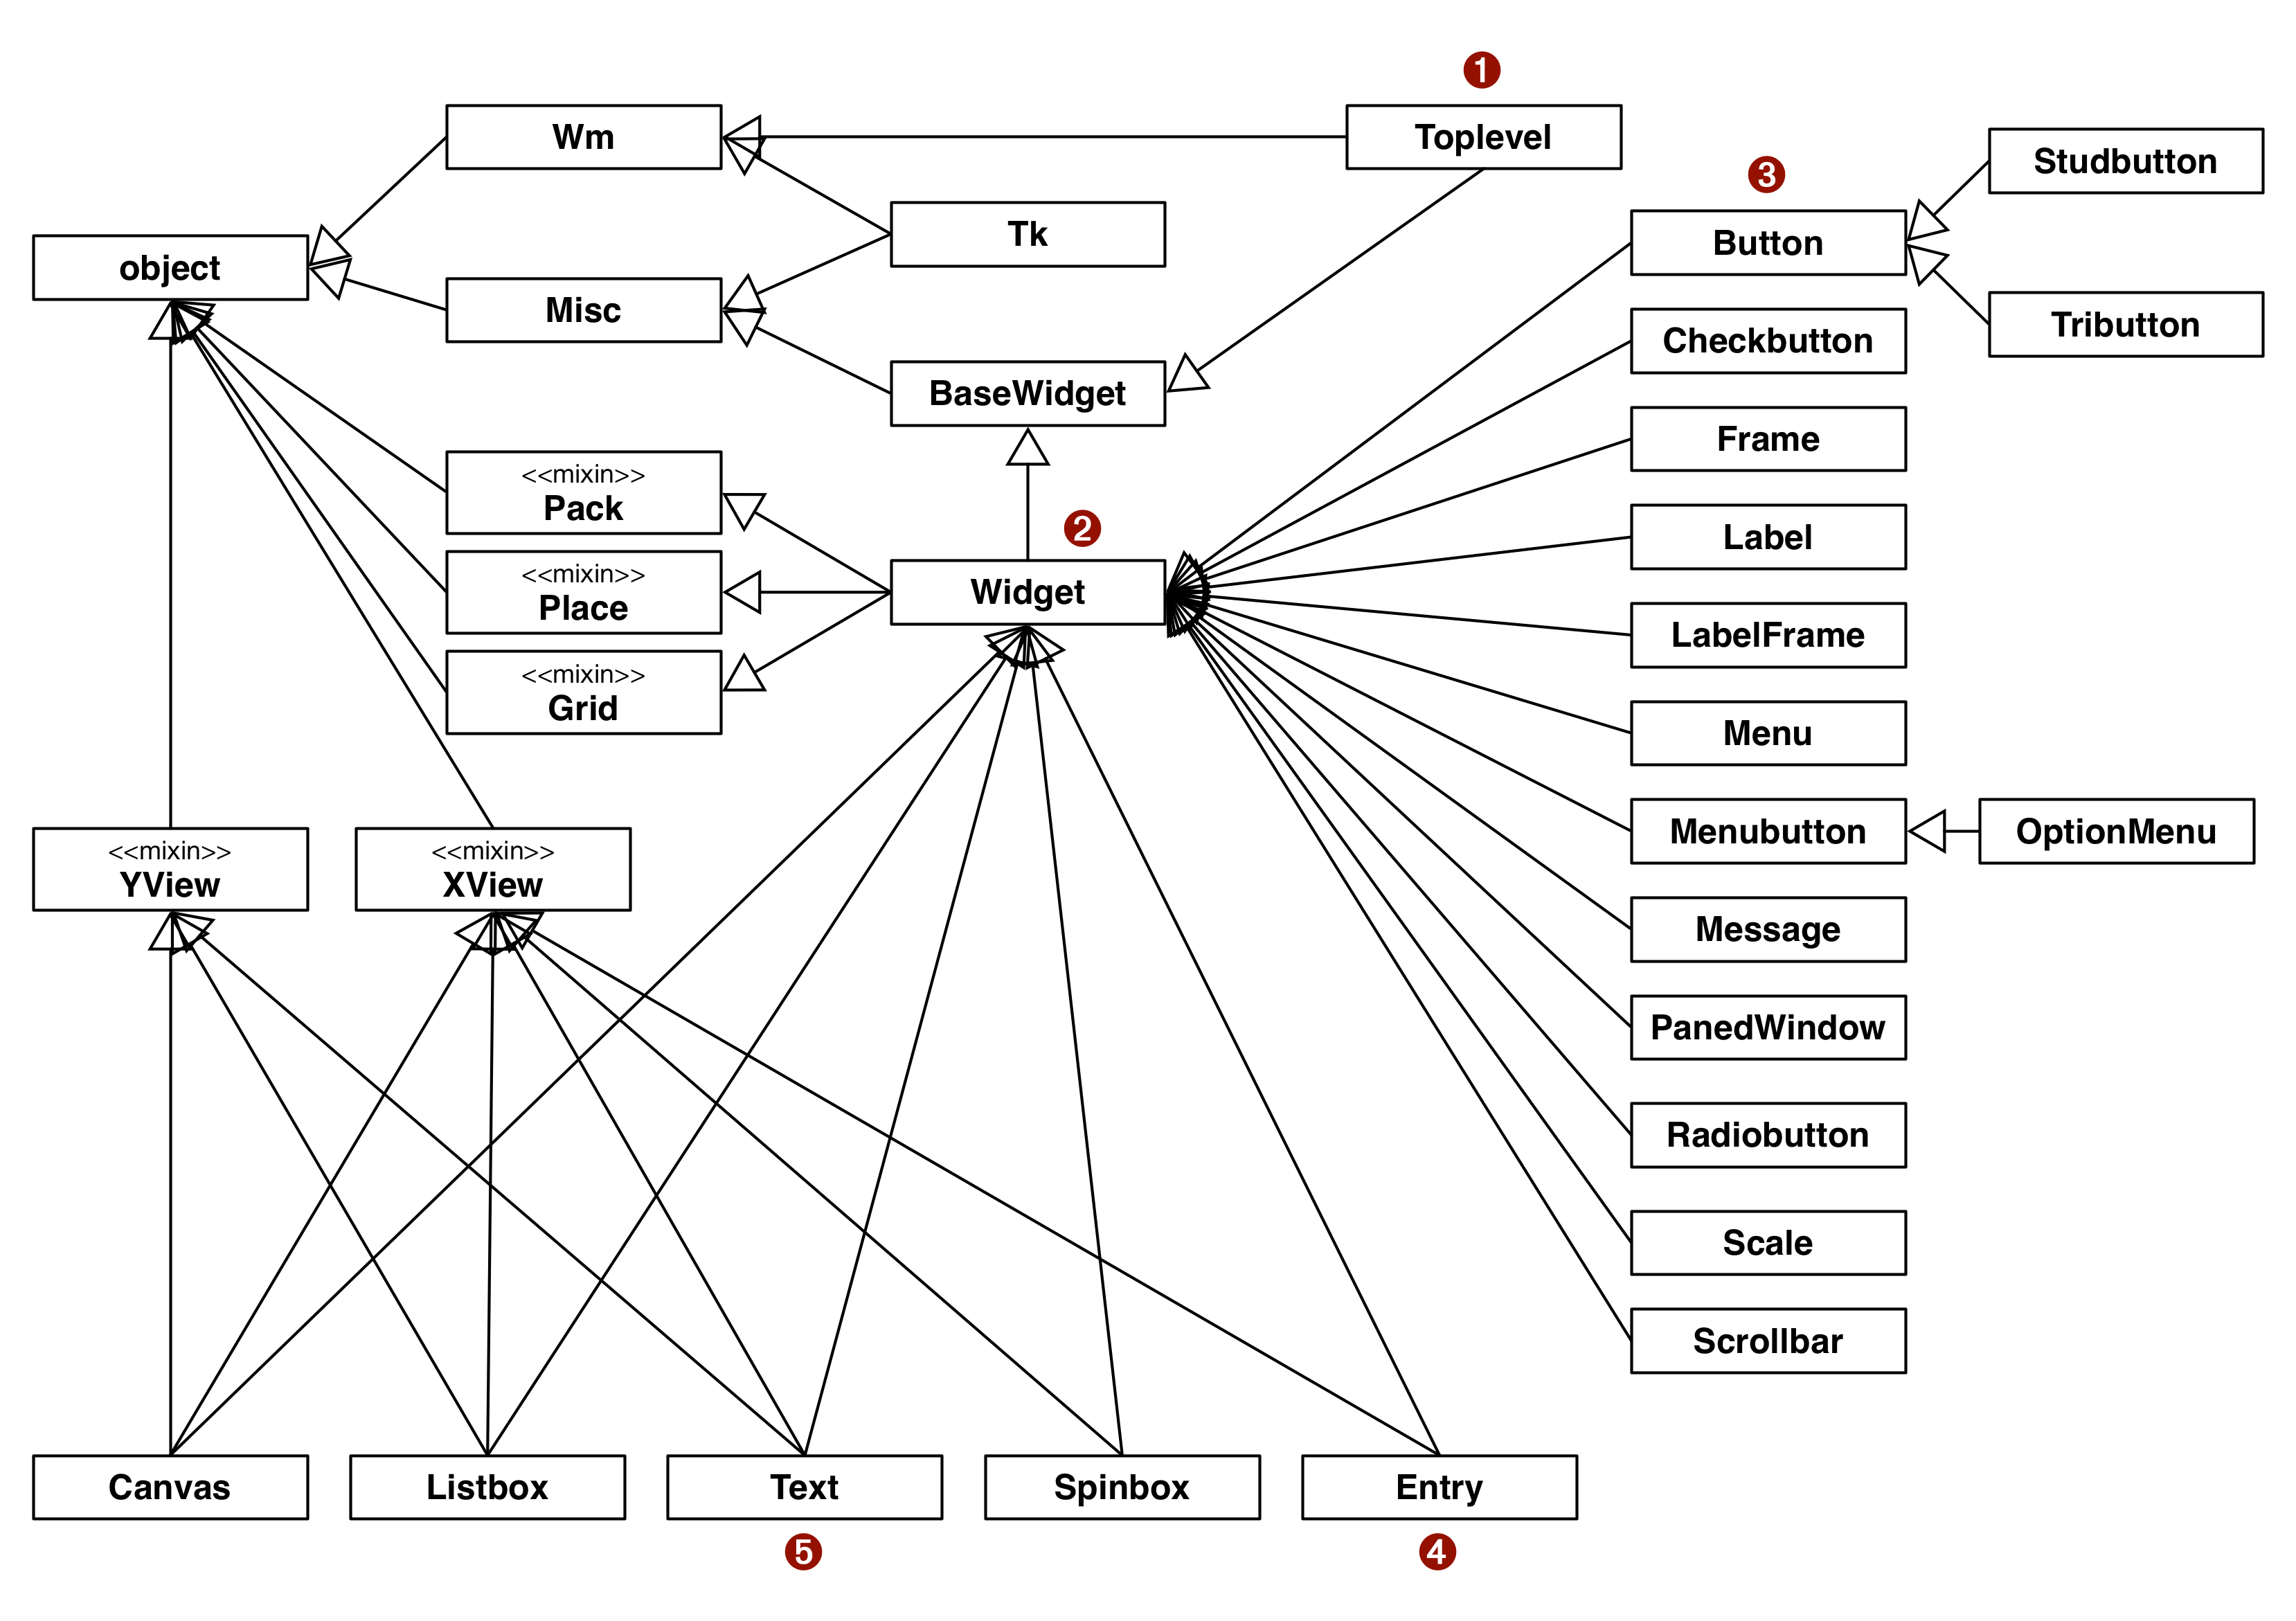
\includegraphics[width=0.6\textwidth]{tk-widgets.png}
\end{center}

\subsection{Composition}
\textbf{Composition} is a different technique for reusing functionalities. The concept is simple: just use an object of some class as a member of a different one. For example we can create the classes \texttt{Engine} and \texttt{Wheel} and then the class \texttt{Car} will have a member of type \texttt{Engine} and 4 members of type \texttt{Wheel}. A class like \texttt{Car} in the example is sometimes called an \textbf{aggregate} class. Here is how you might implement this composition in Python:

\input{pygments/composition}

\subsubsection{Composition vs Inheritance}
Composition models a \textbf{'has-a'} relation in the real world: a \texttt{Car} \emph{has} an \texttt{Engine}. Inheritance models a \textbf{'is-a'} relation in the real world: an \texttt{Electron} \emph{is} a \texttt{Particle}. It may not always be obvious which one to use in your specific case, so choose wisely.

Just remember that inheritance is a wild beast. There are entire libraries written about how and when (not) to use it. Question for you: should a \texttt{Square} inherit from a \texttt{Rectangle}? Seems legit: a \texttt{Square} \emph{is} a specialized \texttt{Rectangle}. But what happens if the \texttt{Rectangle class} has a \texttt{changeHeight()} method?

Always keep in mind the so-called \textbf{Liskov substitution principle}: you should always be able to use a derived class instead of a base class in your code. In other words: \textit{a derived class should always extend or specialize the functionalities of the base class, never restrict them.}

\subsubsection{Short summary 3: Inheritance and composition}
\begin{itemize}
    \item A class can inherit functionalities from one or more other classes (\textbf{Inheritance})
    \item The class that inherits is called \textbf{derived} (or \textbf{child}) class, while the inherited one is the \textbf{base} (or \textbf{parent}) class
    \item Inheritance models an \emph{is-a} relationship
    \item Inheritance is tricky: use it with care and follow the \textbf{Liskov substitution principle}.
    \item Classes can also incorporate other objects as class members (\textbf{Composition})
    \item Composition models a \emph{has-a} relationship
\end{itemize}
\section{OOP introduction: Special methods}

\subsection{Special methods in practice}
Suppose we want to create a class for managing 2D vectors. That's just for learning: there are already plenty of libraries for doing array operations, like \texttt{numpy}. Anyway, let's start coding some useful methods for it. Here is a naive implementation:

\input{pygments/vector2d_naive}

This kind of works but isn't that ugly? Look at the lines \texttt{v.info()} or \texttt{v.module()}. It would be far more readable to just do \texttt{print(v)} and \texttt{abs(v)}. And what about \texttt{t = v.add(z)}? Why not \texttt{t = v + z}?

In Python there is a tool that allows you to do just that: \textbf{special methods}. In the last lesson, we saw that special methods (or dunder methods or magic methods) are methods like \texttt{\_\_init\_\_} and get special treatment by the Python interpreter. There are a few tens of special methods in Python. In the next sections we are going to see how they work. 

\subsection{\texttt{\_\_abs\_\_} \texorpdfstring{$\xrightarrow{}$}{->} \texttt{abs()}}

In the following example, the \texttt{\_\_abs\_\_} method was implemented for our class. Look at the code: note that every object that is an instance of a class with the \texttt{\_\_abs\_\_} method can be the argument of the \texttt{abs()} built-in function. That's exactly what is going to happen for many other special methods.

\input{pygments/vector2d_2}

\subsection{\texttt{\_\_str\_\_} and \texttt{\_\_repr\_\_} \texorpdfstring{$\xrightarrow{}$}{->} \texttt{str()}, \texttt{print()} and \texttt{repr()}}

What about \texttt{print()}? There are actually two special methods used for that: \texttt{\_\_str\_\_} and \texttt{\_\_repr\_\_}. The \texttt{\_\_str\_\_} special method is meant to return a concise string for the user; it is called with \texttt{str()}. The \texttt{\_\_repr\_\_} special method is meant to return a richer output for debugging. It is called with \texttt{repr()}.

\texttt{print()} automatically tries to get a string out of the object using \texttt{\_\_str\_\_}. If there isn't one, it searches for \texttt{\_\_repr\_\_}. A default \texttt{\_\_repr\_\_} is automatically generated for you, if you haven't defined one.

Here is how you can implement these two methods:

\input{pygments/vector2d_printable}

\subsection{Mathematical operations using special methods}
You can easily define mathematical operations by implementing the corresponding special methods, such as \texttt{\_\_add\_\_} or \texttt{\_\_mul\_\_}:

\input{pygments/vector2d_math}

\subsection{In place operations using special methods}
Similarly, in place operations like \texttt{+=} can be implemented using methods such as \texttt{\_\_iadd\_\_}:

\input{pygments/vector2d_inplace}

\subsection{Comparisons using special methods}
To allow comparisons between objects (e.g., using \texttt{==} or \texttt{!=}), you can define methods like \texttt{\_\_eq\_\_} and \texttt{\_\_ne\_\_}:

\input{pygments/vector2d_comparable}
\hrulefill

Here is how you would test these comparison methods:

\input{pygments/test_vector2d_comparable}

\subsection{Creating a hashable object using special methods}
Now let's try to make our \texttt{Vector2d} \textit{hashable}. Hashable objects can be put in \textit{sets} and used as keys for dictionaries.
To make an object hashable we need to fulfill 3 requirements:
\begin{itemize}
    \item[-] It has to be immutable, otherwise you may not retrieve the correct hash;
    \item[-] It needs to implement an \texttt{\_\_eq\_\_} function, so one can compare objects of this class;
    \item[-] It needs a (reasonable) \texttt{\_\_hash\_\_} function.
\end{itemize}
As said in the previous sections, a good hash function must return the same value for objects that compare as equal, should rarely return the same value for different objects and should sample the result space uniformly. Here's how we can make \texttt{Vector2d} hashable:

\input{pygments/vector2d_hashable}
\hrulefill

And this is the resulting behavior in practice:

\input{pygments/vector2d_hashable_test}

\subsection{List-style access using special methods}
2D arrays are boring. Why not an N-d array? Of course we cannot store the components explicitly like before. We need a container for that and we will use \texttt{array} from the \texttt{array} library \footnote{\texttt{array} uses a typecode (a single character) for picking the type of data stored in the array. 'd' is the typecode for float numbers in double precision.}. This is an example of \textit{composition}.

Here is a question for you: why not just use a list or a tuple?

Let's create the new class utilizing the underlying array:

\input{pygments/vector}

Now that we have an arbitrary number of components, we cannot access them like \texttt{vector.x}, \texttt{vector.y}, etc\dots anymore. What we want is a syntax similar to that of lists: \texttt{vector[0]}, \texttt{vector[1]} and so on.

There are two magic methods for that: \texttt{\_\_getitem\_\_} for access and \texttt{\_\_setitem\_\_} for modifying. While we are at it, we will also implement the \texttt{\_\_len\_\_} method, which allows us to call \texttt{len(vector)}. Here's how you do it:

\input{pygments/vector_random_access}
\hrulefill

And here is how we can test the new random access functionality:

\input{pygments/test_vector_random_access}

\subsection{Making an object iterable using special methods}\label{sec:special_iterable}
Now our vector behaves a bit like a native Python list. However, a list has a very powerful feature we miss: it's \textit{iterable}.

An \textbf{iterable} in Python is something that has an \texttt{\_\_iter\_\_} method, which returns an \textbf{iterator}. Technically, an iterator is an object that implements the \texttt{\_\_next\_\_} special method, which is used to retrieve elements one at a time. We will not discuss iterators any further here. Instead, we will just exploit composition and borrow the \texttt{\_\_iter\_\_} method from the underlying array:

\input{pygments/vector_iterable}
\hrulefill

You can verify its iterability as follows:

\input{pygments/vector_iterable_test}

\hrulefill

\subsubsection{Note: Duck typing and polymorphism}
The duck test: "\textit{If it looks like a duck and quacks like a duck, it must be a duck.}".

When programming, Python usually doesn't care about the type of an object but only what the object \textit{can do} (i.e. its methods). That is the concept of \textbf{duck-typing}, shown in this classic example:

\input{pygments/duck_typing}

In statically typed languages\footnote{Statically typed languages: type-checking happens at compile-time. Dynamically typed languages: type-checking happens at runtime.} like Java, C or C++ this is typically done with inheritance, e.g. we make \texttt{Duck} and \texttt{Goose} inherit from a base class \texttt{QuackingBird()} or something like that. That is because functions from statically typed languages always require arguments of a specific type.

Python (like JavaScript) is dynamically typed, so we can use duck typing for that. We just need to implement the \texttt{quack()} method for both \texttt{Duck()} and \texttt{Goose()} and we are done. In other words we obtain polymorphism (which is the act of using objects with different types for the same function) just by satisfying the required \textit{interface} (in this case the \texttt{quack()} function).

\hrulefill

Having an iterable \texttt{Vector} (thanks to the \texttt{\_\_iter\_\_} magic method) makes all the difference in the world. There are \emph{a lot} of built-in and library functions in Python accepting a generic iterable as input:
\begin{itemize}
    \item[-] \texttt{sum}: Sum all the elements
    \item[-] \texttt{max}/\texttt{min}: Return the maximum/minimum
    \item[-] \texttt{reversed}: Loop in the reversed order
    \item[-] \texttt{all}: Return true if a given condition is true for all the elements
    \item[-] \texttt{any}: Return true if a given condition is true for at least one element
    \item[-] \texttt{functools.reduce}: Apply a function recursively to pairs of elements
    \item[-] \texttt{enumerate}: Iterate with automatic counting of iterations
    \item[-] \texttt{map}: Apply a function to the elements one by one
    \item[-] \texttt{filter}: Iterate only on the elements passing a given condition
    \item[-] \texttt{zip}: Iterate over pairs of elements (requires two iterables)
\end{itemize}

Countless others can be found in the \texttt{itertools} library:
\begin{itemize}
    \item[-] \texttt{islice}: Slice the loop with start, stop and step
    \item[-] \texttt{takewhile}: Stop looping when a condition becomes false
    \item[-] \texttt{accumulate}: Get the results of applying the function iteratively to pairs of elements
    \item[-] \texttt{chain}: Loop through many sequences one after another
    \item[-] \texttt{cycle}: Loop over the sequence repeatedly, indefinitely
    \item[-] \texttt{permutations}: Get all the permutations of a given length
    \item[-] \texttt{product}: Compute the cartesian product of iterables
    \item[-] \texttt{groupby}: Group by value of some key (function)
    \item[-] \dots
\end{itemize}

Thanks to duck typing, we can now use any of that for our \texttt{Vector} class.

\input{pygments/vector_ducked}
\hrulefill

Here is a demonstration of our iterable vector interacting with Python's built-in functions:

\input{pygments/test_vector_ducked}

\subsection{Callables and functions: the \texttt{\_\_call\_\_} special method}
Remember that in the past lessons you were told that functions are objects of the \texttt{function} class. How are they implemented? With a special method of course: \texttt{\_\_call\_\_}. Every object implementing a \texttt{\_\_call\_\_} method is called \textbf{callable}. In this example the object \texttt{line} is a callable, so we can write \texttt{line(2.)}, just like a normal function.

\input{pygments/callable_line}

Let's create for example a call counter, which is a class that counts how many times a function is called in your code. Then we implement a simple fit and count the function calls during the fitting operations.

\input{pygments/callable}
\hrulefill

And here is how it behaves during a fitting procedure:

\input{pygments/test_callable}

\begin{center}
    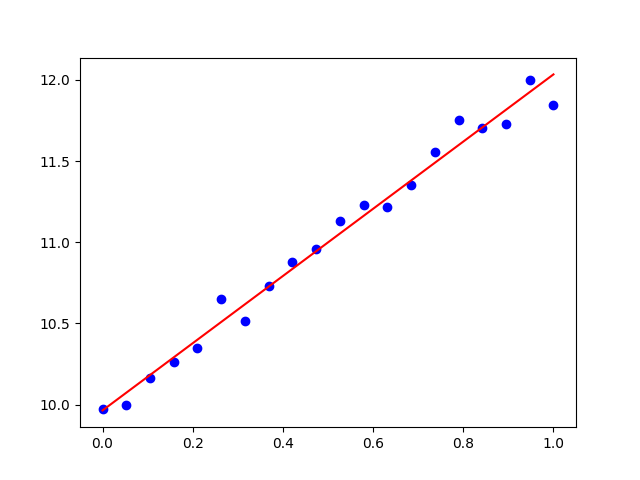
\includegraphics[width=0.5\textwidth]{fit_with_custom_callable.png}
\end{center}

\subsubsection{Short summary 4: Special methods}
\begin{itemize}
    \item \textbf{Special methods} can be used to greatly enhance the readability of the code and get your classes to behave in an appropriate way.
    \item There are tens of special methods in Python, covering logical operations, mathematical operations, array-style access, iterations, formatting and many other things.
    \item By implementing the required interface in your classes, you will be able to reuse a lot of code written for the standard containers thanks to \textbf{duck typing}, which is the pythonic way to polymorphism.
\end{itemize}
\section{The \texttt{numpy} module, vectorization and other miscellanea}

\subsection{Introduction to \texttt{numpy}}
As a data scientist, the \texttt{numpy}, \texttt{pandas} and \texttt{scipy} modules will be your best friends.
Among many other things, \texttt{numpy} offers:
\begin{itemize}
    \item[-] a powerful n-dimensional array object;
    \item[-] mathematical functions that interoperate natively with arrays.
\end{itemize}
\texttt{scipy} provides the user with powerful functions for:
\begin{itemize}
    \item[-] numerical integration;
    \item[-] optimization (a.k.a. fitting);
    \item[-] interpolation;
    \item[-] signal processing.
\end{itemize}
Finally, \texttt{pandas} is the best tool to interoperate your code with Excel.

In this section we will sum up some of the most important functions, objects and capabilities of the \texttt{numpy} library. As a fellow Python user, you should be familiar with the basics, so we will fly through the first introductory snippets of code and focus more on the concept of vectorization.

\subsection{Basics of \texttt{numpy}}
\subsubsection{- \texttt{numpy} arrays}
Let's start by reviewing how to create and manipulate basic \texttt{numpy} arrays:

\input{pygments/numpy_arrays}

\subsubsection{- \texttt{numpy} arrays vs. Python lists}
Arrays and lists are fundamentally different objects:
\begin{itemize}
    \item[-] They have a different footprint in memory, and operate at different speeds;
    \item[-] Arrays are homogeneous (which means that each element is of the same type), lists don't need to be;
    \item[-] Arrays offer a much more powerful indexing/slicing method;
    \item[-] Arrays interoperate with \texttt{numpy} mathematical functions.
\end{itemize}

Here is a code snippet demonstrating some of these differences:

\input{pygments/numpy_arrays_vs_lists}

\subsubsection{- Broadcasting}
Broadcasting is a powerful mechanism that allows \texttt{numpy} to work with arrays of different shapes when performing arithmetic operations:

\input{pygments/numpy_arrays_broadcasting}

\subsubsection{- Mathematical functions in \texttt{numpy}}
Here are some examples of how mathematical functions are applied to arrays:

\input{pygments/numpy_functions}

\texttt{numpy} mathematical functions interoperate natively with arrays (and work on plain old numbers, too). Under certain conditions, \texttt{numpy} can make operations on arrays of different shapes. This is extremely useful when vectorizing problems.

\subsubsection{- Arrays and masks}
Masks are a powerful tool in \texttt{numpy}. They can replace conditional expressions in a for loop in a vectorization context (more on this later). The following example shows how masks can be applied:

\input{pygments/numpy_masks}

\subsection{Vectorization}

Python is known to be slow. This is the price you pay for being so beautiful and flexible. Does it matter? It depends on the situation. If you are parsing a text file or fetching a web page, then probably not, but if you are performing CPU-intensive processing on a TB of data, probably yes.

What's so magical about using \texttt{numpy}? \texttt{numpy} is written in C as a Python extension, so routines are highly optimized to crunch numbers. When you perform an array operation in Python you are actually executing optimized C code. Here comes \textbf{vectorization}, which is the practice of substituting explicit \texttt{for} or \texttt{while} loops with operations on arrays. If you are working with large amounts of data you must find a way to vectorize your processes. Of course, not every problem can be vectorized, but the ones that can will surely experience a significant speed-up.

\textbf{Basic message: avoid loops in pure Python when crunching numbers and vectorize your problems (if you can)}.

To illustrate the power of vectorization, consider this comparison between a standard loop and a vectorized approach:

\input{pygments/vectorization}

\subsection{Pseudo-random number generators}
Every programming language comes with a Pseudo Random Number Generator (PRNG) that produces random floats uniformly in $[0.0,~1.0)$. Python is no exception: 
\begin{verbatim}
import random
x = random.random()
\end{verbatim}
Here's the link for the \texttt{random} library documentation: \url{https://docs.python.org/3/library/random.html}. \texttt{numpy} itself has a PRNG, that you can find in the \texttt{numpy.random} module.

PRNGs are an interesting (and fun) subject by themselves. See for example:
\begin{itemize}
    \item[-] Donald E. Knuth, \emph{The Art of Computer Programming, Volume 2: Seminumerical Algorithms}, 3rd Edition
    \item[-] M. Matsumoto and T. Nishimura, \emph{Mersenne Twister: A 623-dimensionally equidistributed uniform pseudorandom number generator}, ACM Transactions on Modeling and Computer Simulation Vol. 8, No. 1, January pp.3--30 1998.
\end{itemize}

\subsection{Generating points with fixed PDF using PRNGs}

\footnote{These next two sections were surely NOT generated by AI starting from the lesson slides. How could you think something like that?!} Let's say we want to simulate the results of the measurements of a certain quantity $x$ knowing its Probability Density Function (PDF) $p(x)$.

\subsubsection{Method 1: The Rejection Method (Hit or Miss)}

\begin{center}
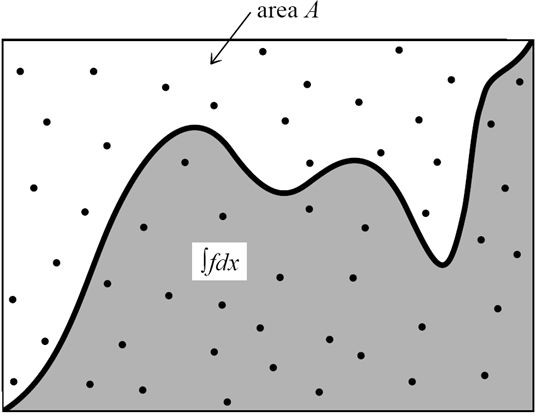
\includegraphics[width=0.5\textwidth]{hitmiss}
\end{center}
The "Hit or Miss" approach, formally known as the \textbf{Rejection Method}, is a geometric strategy. The idea is to enclose your target PDF inside a bounding box (or a simpler distribution) that is easy to sample from.

\begin{enumerate}
    \item Generate a candidate $x$ from the bounding box.
    \item Generate a random height $y$.
    \item \textit{Accept} the candidate if $y \leq p(x)$ (the point falls "under" the curve).
    \item \textit{Reject} it otherwise.
\end{enumerate}

While conceptually simple, this method is often computationally inefficient because many generated points are discarded, especially if the bounding box creates a large empty area above the curve.

\subsubsection{Method 2: Inverse Transform Sampling}
A much more elegant and efficient approach is the \textbf{Inverse Transform Sampling}. Instead of throwing points and hoping they land correctly, we leverage the mathematical properties of the Cumulative Distribution Function (CDF).

Let us define the fundamental components:
\begin{itemize}
    \item[-] \textbf{PDF ($p(x)$):} The probability density we want to simulate.
    \item[-] \textbf{CDF ($F(x)$):} The integral of the PDF, representing the probability that a variable takes a value less than or equal to $x$:
    \begin{equation}
        F(x) = \int_{-\infty}^{x} p(x') \, dx'
    \end{equation}
    Since it is a probability, the range of $F(x)$ is always $[0, 1]$.
\end{itemize}

The core idea relies on the \textit{Percent-Point Function (PPF)}, which is simply the inverse of the CDF: $x = F^{-1}(q)$.

There is a fundamental theorem stating that:
\begin{quote}
    \textit{If $q$ is a uniformly distributed random number in $[0, 1]$, then the variable $x = F^{-1}(q)$ is distributed according to $p(x)$.}
\end{quote}

This means we can transform a simple uniform random number (which any computer can generate easily) into a complex distribution just by passing it through the inverse CDF.

To implement this method in a real scenario, follow these three steps:

\begin{enumerate}
    \item \textit{Integrate:} Calculate the CDF, $F(x)$, by integrating your target PDF.
    \item \textit{Invert:} Algebraically solve the equation $y = F(x)$ for $x$. This gives you the inverse function $x = F^{-1}(y)$.
    \item \textit{Sample:}
    \begin{itemize}
        \item[-] Generate a random number $u$ from a uniform distribution ($0 \le u \le 1$).
        \item[-] Compute your target value: $x_{target} = F^{-1}(u)$.
    \end{itemize}
\end{enumerate}

\underline{Practical example: the exponential distribution} \\
Let's see how this translates into practice. Suppose we want to sample from $p(x) = \lambda e^{-\lambda x}$ (for $x \ge 0$).
\begin{enumerate}
    \item Find the CDF: $F(x) = \int_0^x \lambda e^{-\lambda t} dt = 1 - e^{-\lambda x}$.
    \item Invert: Set $u = 1 - e^{-\lambda x}$. Solving for $x$, we get $x = -\frac{\ln(1-u)}{\lambda}$.
    \item Code it: Generate a series of random numbers $u$  and plug them into the formula above. The result is a series of numbers with the desired PDF.
\end{enumerate}

\begin{comment}
\subsection{How do I throw PRN with arbitrary pdf? (Hit or miss)}
\centering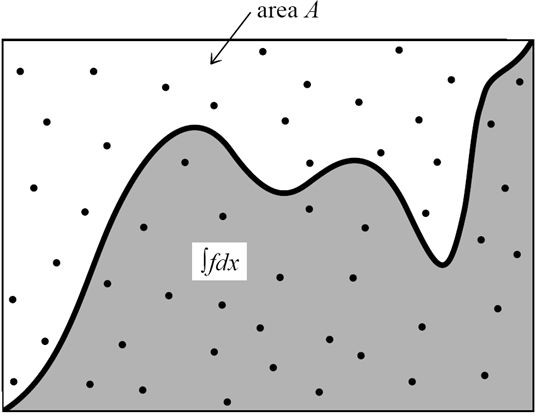
\includegraphics[width=0.5\textwidth]{hitmiss}

\begin{itemize}
    \item Hit or miss, aka acceptance/rejection method:
    \begin{itemize}
        \item Enclose your pdf in a rectangle
        \item Throw a $x$ and a $y$
        \item Accept $x$ if $y \leq f(x)$
    \end{itemize}
    \item \textbf{This is horrible---please don't use it!}
\end{itemize}

\subsection{How do I throw PRN with arbitrary pdf? (Inverse transform)}
\begin{itemize}
    \item Probability density function (pdf)
    $$
    p(x) \quad (\ge 0)
    $$
    \item Cumulative function (cf)
    $$
    F(x) = \int_{-\infty}^{x} p(x') dx'
    $$
    \item Percent-point function (ppf)
    $$
    x = F^{-1}(q)
    $$
    \item \textbf{Awesome fact: if $q$ is uniformly distributed in $[0, 1]$, then $x = F^{-1}(q)$ is distributed according to $p(x)$!}
\end{itemize}
\end{comment}

\subsection{An interesting object: splines}

Spline interpolation represents a sophisticated alternative to global polynomial fitting, designed to avoid the oscillatory instability often seen with high-degree polynomials (Runge's phenomenon). 

Instead of using a single function for the entire dataset, a spline is defined \textbf{piecewise}: the interval between two consecutive data points is bridged by a low-degree polynomial, most commonly a cubic one ($k=3$). 
Crucially, these segments are not isolated; they are mathematically "glued" together at the control points (knots) by enforcing continuity not just of the function itself, but of its first $k-1$ derivatives. This ensures the resulting curve is smooth and differentiable everywhere.

\begin{center}
    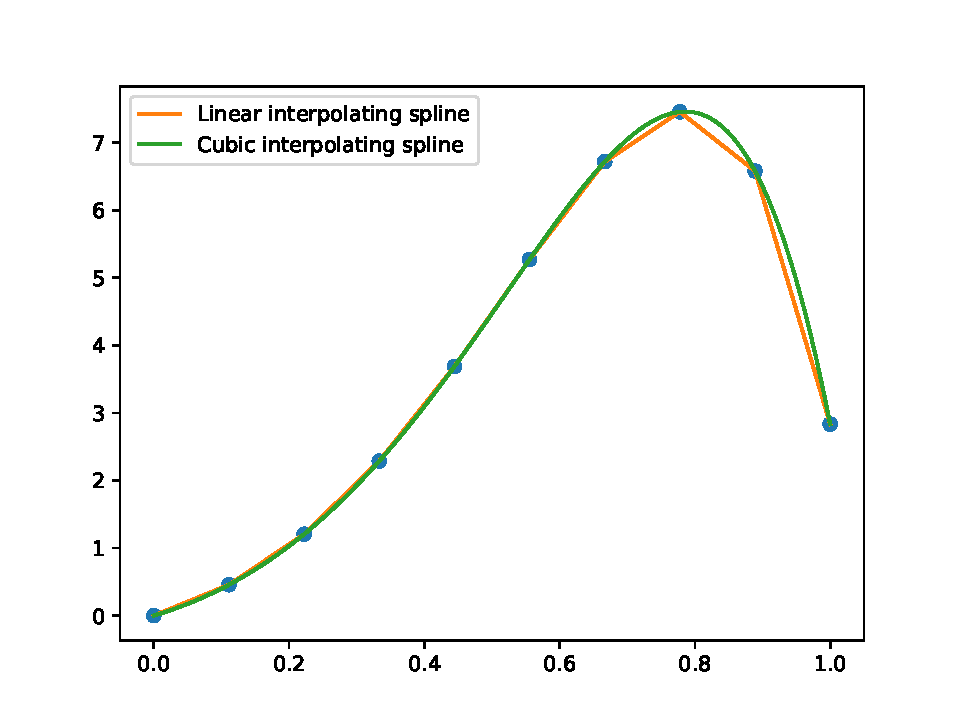
\includegraphics[width=0.6\textwidth]{spline}
\end{center}

From a computational standpoint, splines are extremely efficient. Provided that the input $x$-array is sorted, the specific polynomial segment corresponding to a query point can be located via a binary search, resulting in a complexity of $\mathbf{O(\log N)}$. 

Since the underlying structure is purely polynomial, analytical operations such as differentiation and integration can be computed \emph{exactly} using elementary arithmetic, without the need for numerical approximation.

Here is how you can perform spline interpolation in Python using \texttt{scipy}:

\input{pygments/spline}

\subsection{References}
\begin{itemize}
    \item[-] \url{https://numpy.org/}
    \item[-] \url{https://www.scipy.org/}
    \item[-] \url{https://pandas.pydata.org/}
    \item[-] \url{https://docs.scipy.org/doc/numpy/reference/arrays.indexing.html}
    \item[-] \url{https://docs.scipy.org/doc/numpy/user/basics.broadcasting.html}
    \item[-] \url{https://docs.scipy.org/doc/scipy/reference/interpolate.html}
\end{itemize}














%\end{comment}

% -------------------------------------------------------------------
% PART II: ADVANCED
% -------------------------------------------------------------------
\chapter[Advanced Python concepts]{Advanced Python concepts \\[0.5ex] \large \textit{(Prof. Baldini, Prof. Rizzi)}}

%\begin{comment}
\section{Testing and documentation}

\subsection{Introduction to testing}

\textit{"How do I make sure my program is correct?"}. The short answer is: in real life you don't, especially if your code is asynchronous \footnote{\textit{Asynchronous programming} allows a program to initiate a long-running task (such as an I/O operation) and remain responsive to other events while waiting.}. That is not the same as saying there is nothing you can do. For compiled languages the compiler will flag all obvious and non-obvious mistakes. This doesn't really apply to Python, since Python is interpreted, although the interpreter will stop upon syntax errors.

Besides paying attention, there are two things that you can do even in interpreted languages:
\begin{enumerate}
    \item \textit{Unit testing}
    \item \textit{Static analysis}
\end{enumerate}
Generally people hate both, but they should come right next to version control in your work-flow toolbox.

\subsection{Unit testing in practice}

While programming you should break up your code in many small pieces (or units) which should encapsulate a well-defined and (possibly) simple functionality. This is usually accomplished by means of a sensible hierarchy of functions and classes is typically the hardest task when structuring your code. Also, your code will evolve with time, so you will find yourself \textbf{refactoring code} from time to time. Remember to be DRY: don't repeat yourself.

\textbf{Unit testing} consists in making sure that each single unit is correct by implementing a series of basic checks. You know what each elementary piece of code is suppose to be so make sure it does and, more specifically, make sure it does \textit{with any valid input}! This is much simpler that testing the whole program at once (although you have to do that, too).

Unit testing is so important that many programmers embrace a practice called \textit{Test-Driven Development (TDD)}:
\begin{enumerate}
    \item Write an empty placeholder for your new function;
    \item Write all the unit tests (they will fail);
    \item Implement your function and tweak it until all the tests pass:
\end{enumerate}
You don't need to do that, but imagine how fundamental unit testing is if tests can come before the code itself!

Take a look at this simple example:

\input{pygments/unit_test_naive}


This is fine, but everything happens manually. You have to run the script yourself and you have to inspect the output yourself. As your code grows in complexity, this is not very effective. Thankfully, Python has it's own module for unit testing: \texttt{unittest}. Here's how it works:

\input{pygments/unit_test}

This is much better! The base \texttt{TestCase} class offers all the goodies for unit testing (\texttt{assertTrue()}, \texttt{assertFalse()}, \texttt{assertEqual()}, \texttt{assertAlmostEqual()} etc\ldots).

The execution can be easily made automatic: put all your unit test modules into a test folder, run \texttt{python -m unittest discover} (or, even better, write a small Makefile or .bat script to do that and that's it: all your tests will run in sequence.

Did you just find a bug in your code? Make sure you add a unit test along with the fix, so that you'll never be hurt again by that particular bug. Are you adding a new feature? Make sure the new code is covered by unit tests. You should not be obsessed by the coverage, but you should definitely aim for it to be as large as possible.

When you use \texttt{git} you must remember this: \textbf{you should always make sure that all the unit tests are passing before merging stuff on the master}. More about this in a bit when we'll be talking about continuous integration.

As usual, take a look at this URL and focus on how \texttt{git} and GitHub can handle unit testing: \url{https://lucabaldini.github.io/metarep/setup.html}.

\subsection{Static code analysis}
By its very nature, Python will show you all the errors at runtime. Say you have a bug in a part of the code that is exercised very rarely, and not covered by unit tests. Python might crash the first time you exercise it or it might happily do something that is not what you intended. It might take years for even realizing that there is a bug.

Many common mistakes can be found by just looking at the code, and in fact all of them can, at least in principle. \textbf{Static code analysis} is just that: searching for errors \textit{before} running the code. Part of it can be done programmatically. Generally, a program will not \textit{understand} your program, but a program can be trained to spot some kind of errors and inconsistencies. \texttt{Pylint} and \texttt{pyflakes} are good examples of such tools. 

Let's say that you want to inspect this code using \texttt{Pylint}.

\input{pygments/linting1}

You will run \texttt{pylint file\_name.py} and you will see the following output in the terminal. As you can see, \texttt{Pylint} finds your mistakes and tells you where you've made them. It also gives a mark to your code just to humiliate you a little more.

{\scriptsize
\begin{verbatim}
[lbaldini@nbbaldini latex]$ pylint snippets/linting1.py 
************* Module snippets.linting1
snippets/linting1.py:1:0: C0111: Missing module docstring (missing-docstring)
snippets/linting1.py:1:0: C0103: Constant name "x" doesn't conform to UPPER_CASE
                          naming style (invalid-name)
snippets/linting1.py:2:0: C0103: Constant name "y" doesn't conform to UPPER_CASE
                          naming style (invalid-name)
snippets/linting1.py:3:0: C0103: Constant name "very_uncommon_condition" doesn't
                          conform to UPPER_CASE naming style (invalid-name)
snippets/linting1.py:5:14: E0602: Undefined variable 'z' (undefined-variable)

--------------------------------------------------------------------
Your code has been rated at -5.00/10 (previous run: -5.00/10, +0.00)
\end{verbatim}
}

\textit{You should consider using static code analysis routinely}. Static analysis tools tend to be quite verbose, and often times verbose is the same as annoying. They try and enforce many different good things at once, such as:
\begin{itemize}
    \item formal correctness;
    \item efficiency;
    \item avoiding anti-patterns;
    \item style guides;
    \item generic conventions.
\end{itemize}
They also are typically highly customizable. i.e., you can mute errors you don't care about. But be advised: most of the times you should probably care. Finding a good balance is generally not too hard and it will surely help you in the long run.

One more thing: recent Python 3 versions support type annotations. \textit{The Python interpreter recognizes but does nothing with annotations}, but they can be handy as comments are. The code is easier to read and even more checks with respect to an un-annotated code can be done by tools such as \texttt{mypy}.

\input{pygments/type_annotation}

\subsection{Continuous integration}
Wouldn't it be nice if somebody run all the unit tests of my package every time I push on the master or make a pull request? And, since we are at it, sent me an email if any of the tests fail? Well, such a thing exists and it is standard practice in code development. People even made a name for it: \textbf{Continuous Integration (CI)}.

CI cloud-base services exists just like code-hosting services exist. Travis-CI and circleci are two good examples. They interoperates seamlessly with GitHub, gitlab or bitbucket. Setting up CI for your package is usually fairly simple, you can find out how to do it (you guessed it) here: \url{https://lucabaldini.github.io/metarep/setup.html}. \\ \textbf{One-sentence summary: always implement continuous integration!}

\subsection{Documentation and Sphynx}

\begin{figure}[H]
\centering
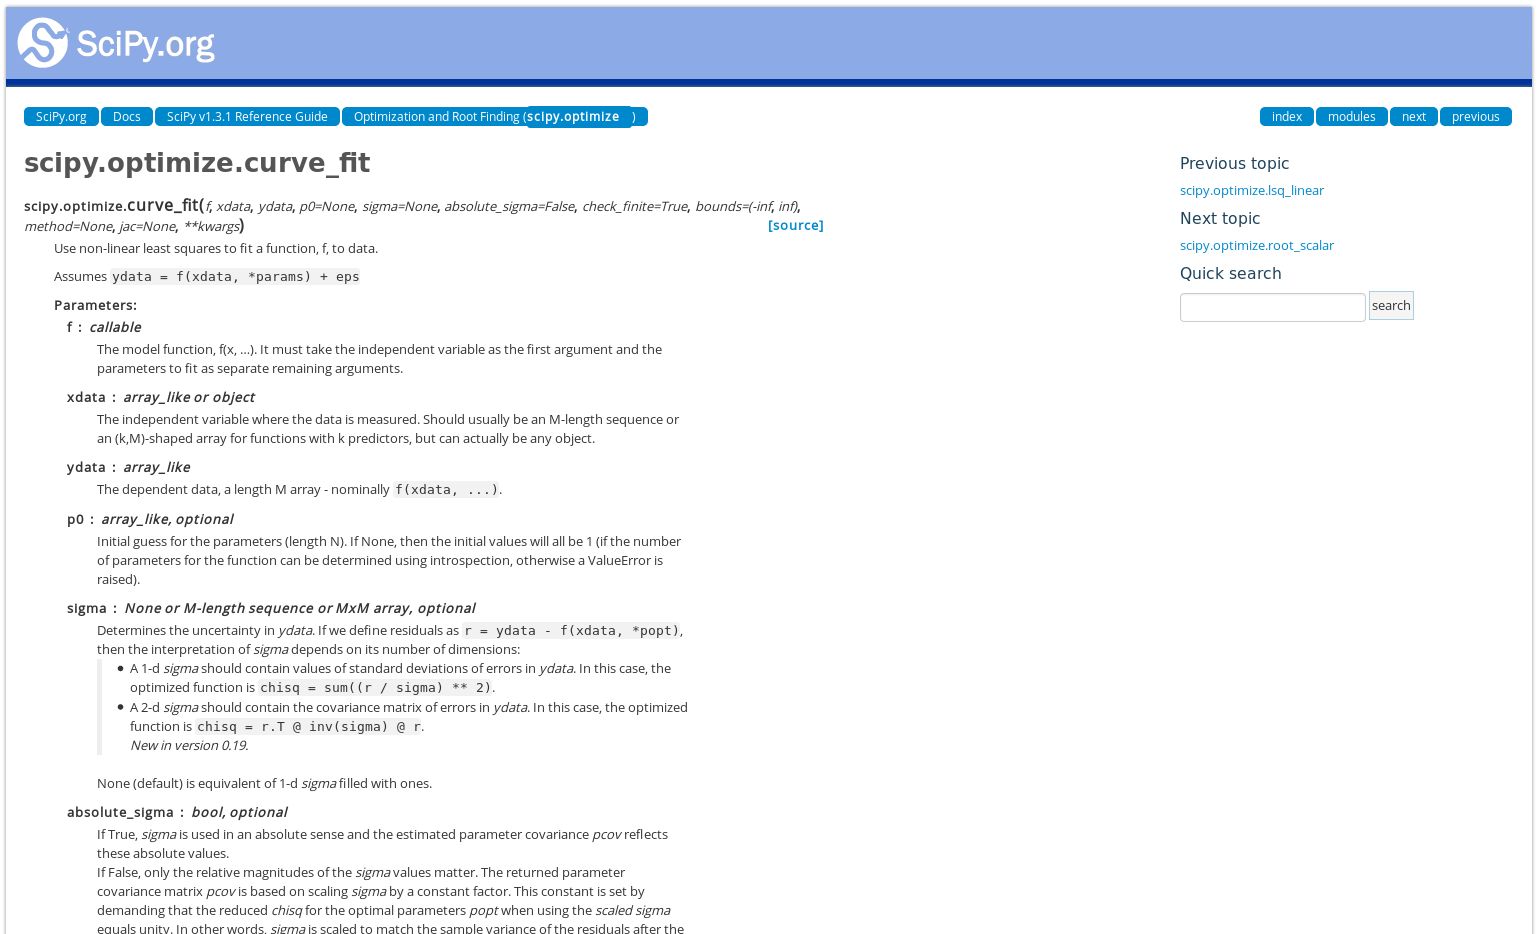
\includegraphics[width=0.6\textwidth]{curve_fit_docs}
\end{figure}

Take a look at the page containing the documentation of the \texttt{curve\_fit} function from the \texttt{scipy.optimize} module. How can it be automatically generated? If you open the source code you'll notice that the documentation is written directly as a docstring in Python.

\begin{figure}[H]
\centering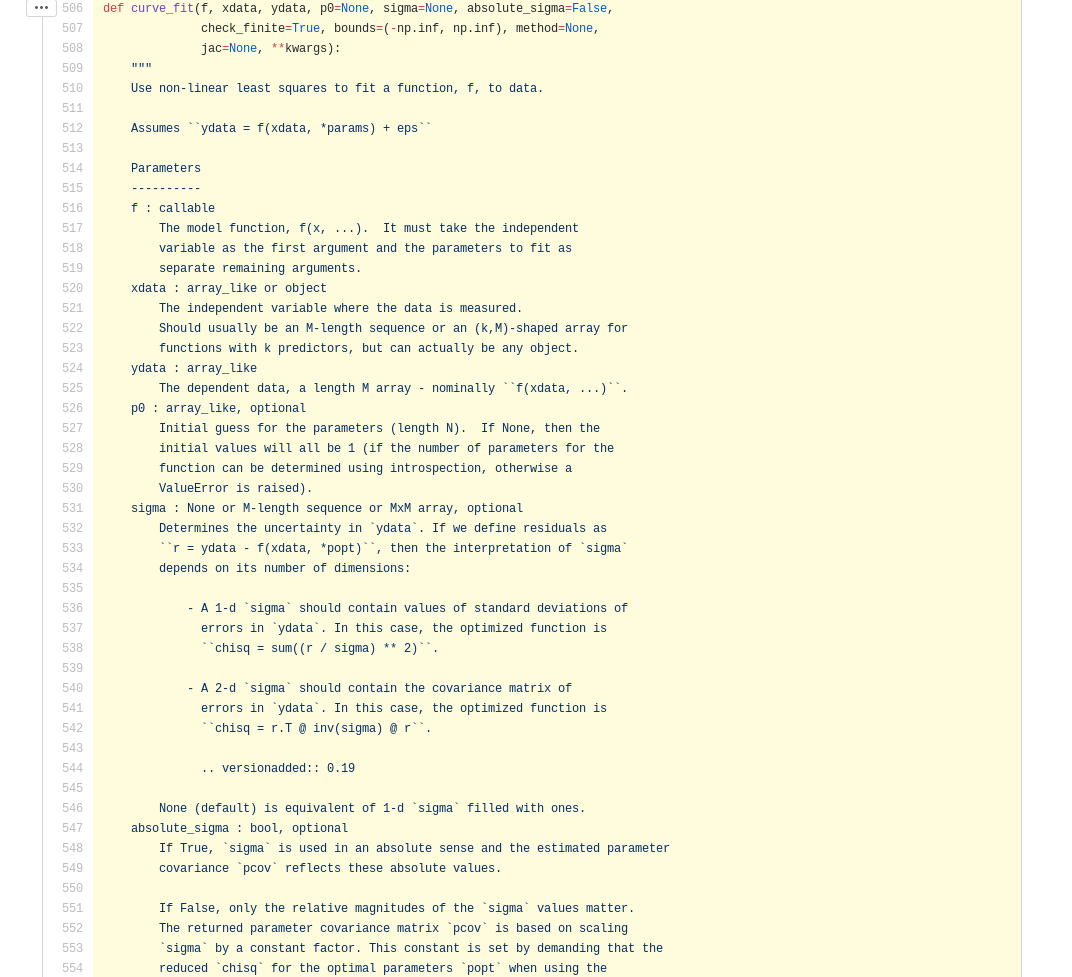
\includegraphics[width=0.6\textwidth]{curve_fit_code}
\end{figure}

\textbf{Sphinx} is the documentation tool for Python. You must learn to use it and love it. 

\begin{figure}[H]
\centering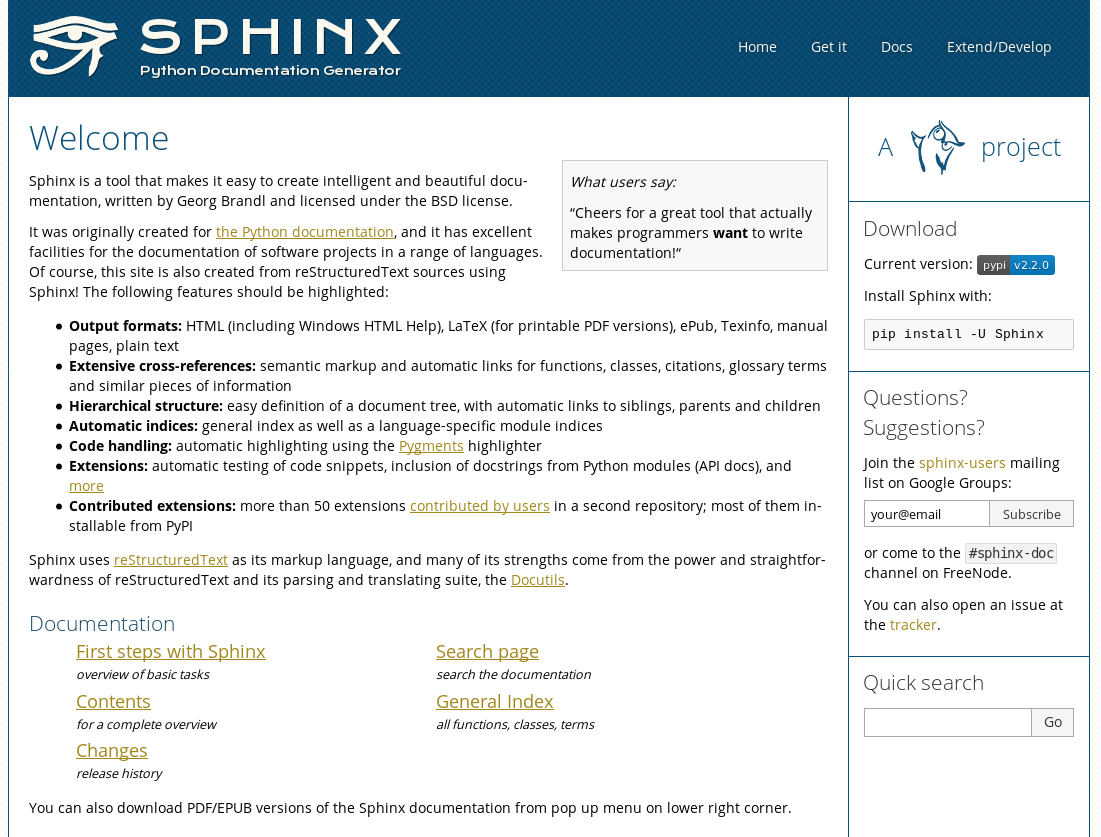
\includegraphics[width=0.6\textwidth]{sphinx}
\end{figure}

Sphynx automatically processes all the relevant information to produce several types of output, most notably html and LaTeX. It considers two different sources of information:
\begin{enumerate}
    \item The doctrings in the Python modules;
    \item The additional markup files (written in \texttt{reStructuredText}) containing auxiliary information.
\end{enumerate}
Use \texttt{sphinx-quickstart} once when you setup your project and then weak the generated \texttt{conf.py} file to suit your needs. You probably don't want to see this link anymore, but here you can learn how to use Sphinx in practice: \url{https://lucabaldini.github.io/metarep/setup.html}.

Sphinx is \textit{very} powerful: the Python documentation itself (\url{https://docs.python-guide.org/}) is written in Sphinx, and so is any module documentation.

\textit{"Ok, I have the documentation compiled. Now what do I do with it?"}
Wouldn't it be nice if the documentation was automatically compiled and uploaded on the web each time you push on the master branch? This is possible and is called readthedocs.com. And, again, this is a cloud-based service that can interoperate easily with GitHub, gitlab or bitbucket. How do you do it in real life? Well, here's the link again: \url{https://lucabaldini.github.io/metarep/setup.html}.

\subsection{References}
\begin{itemize}
    \item \url{https://docs.python.org/3/library/unittest.html}
    \item \url{https://www.pylint.org/}
    \item \url{https://pypi.org/project/pyflakes/}
    \item \url{http://mypy-lang.org/}
    \item \url{https://circleci.com/}
    \item \url{https://travis-ci.org/}
    \item \url{http://www.sphinx-doc.org/en/master/}
\end{itemize}
\section{Error handling in Python}

\subsection{Errors and Exceptions}
\textbf{Error handling} is one of the most important problems to solve when designing a program. What should you do when a piece of code fails? What does fail mean? Some examples:
\begin{itemize}
    \item Invalid input e.g. passing a path to a non existent file, or passing a string to a function for dividing numbers
    \item Valid output not found, e.g searching the position of the letter 'd' in the string 'elephant'
    \item Output cannot be find in a reasonable amount of time
    \item Runtime resource failures: network connection down, disk space ended\dots
\end{itemize}

Historically, one can follow one of two philosophies when handling errors:
\begin{itemize}
    \item Return some \textbf{error flag} (in different ways) to tell the user that something went wrong;
    \item Use \textit{exceptions}.
\end{itemize}

\subsection{Error flags and their limits}

A typical convention for programs is to return 0 from the main if the execution was successful and an error code (integer number) otherwise. However this isn't the best practice. Take a look a this example:

\input{pygments/error_flags}

Error codes have their use and thay are fine in some cases, but they suffer from a few issues:
\begin{itemize}
    \item Choosing them is often arbitrary and sometimes it is difficult to make a sensible choice. What if all the numbers can represent meaningful output of the function?
    \item They are cumbersome to use. Which error flag is used by a function? 0? -1? 99999999? You have to go through the documentation for each! If you have a deep hierarchy of functions you have to perform checks and pass the error up at every level!
    \item What if the caller of a function does not check the error flag? The bug can propagate \textit{silently} through its code!
\end{itemize}

\subsection{Exceptions}

With that in mind, we want something that
\begin{itemize}
    \item is clearly separated from the returned output
    \item cannot be silently ignored by the user
    \item is easy to report to upper level without lots of lines of code.
\end{itemize}
This is where \textit{exceptions} come into play:

\input{pygments/exceptions_vs_err_flags}

An \textbf{exception} is an object that can be \textbf{raised} (in other languages also \textit{thrown}) by a piece of code to signal that something went wrong. When an exception is raised, the normal flow of the code is interrupted. The program automatically propagates the exception back in the function hierarchy until it finds a place where the exception is \textbf{caught} and handled. If the exception is never caught, not even in the main, the program crashes \textbf{with a specific error message}. Catching the exception is done in Python with a \texttt{try - except} block, just like this:

\input{pygments/exceptions_brief}

There are two more optional statements in a \texttt{try-except} block:
\begin{itemize}
    \item \texttt{else}: contains a piece of code that is executed only if no exception is raised in the try block;
    \item \texttt{finally}: contains a piece of code that is executed no matter what.
\end{itemize}
\texttt{finally} is executed even if there is a return statement in the try block and can be used to release important resources (e.g. closing a file, or a connection).

\input{pygments/exceptions}

If that was all, exceptions would only be moderately useful. The real bargain is that \textit{you can send back information} together with the exception. In fact you \textit{are sending a full object}: the exception itself. Inside the exception you can report all kind of data useful to reconstruct the exact error, which can be used by the caller for debugging or to produce meaningful error messages. You can also select which exceptions you catch, leaving the others propagating up, as done in this example: 

\input{pygments/try_block}

Python provides a rich hierarchy of exception classes, which you can further customize (if you want) by deriving your own subclasses. Here's a schematic representation:
\begin{figure}[H]
\centering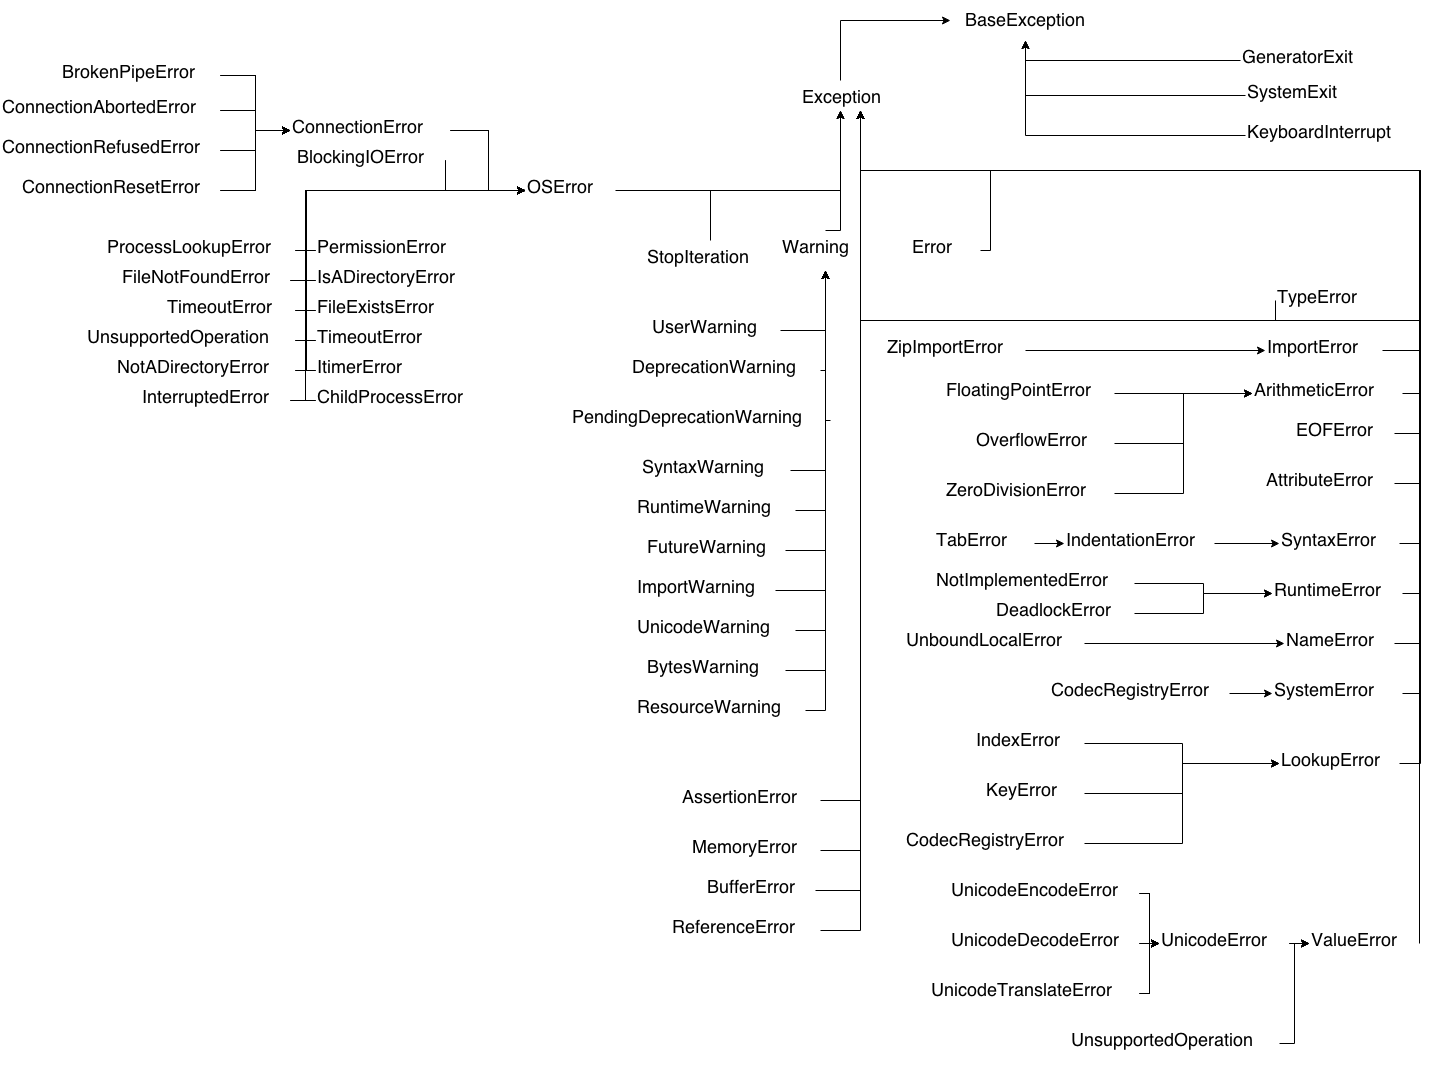
\includegraphics[width=\textwidth]{python_exceptions}
\end{figure}

However, even exceptions have some caveats. For example, catching \texttt{Exception}, will also catch \texttt{SyntaxError} and \texttt{NameError}. This means that the code will 'run' even if there is a typo in it! Bottom line: \textbf{you should never catch generically for \texttt{Exception}}, always be more specific.
Even worse, you should never catch for \texttt{BaseException} as that would even prevent the user from aborting the execution with a \texttt{KeyboardInterrupt} (e.g. Ctrl-C). 

In Python, exceptions are the default methods for handling failures. Many functions raise an exception when something goes wrong. The common approach is: do not check the input beforehand, use it and be ready to catch exceptions if any.

\input{pygments/dont_ask_permission}

\subsection{The traceback}
A \textbf{stack traceback}, or simply traceback, is a list of the function calls at a specific point in the code. An exception always stores the traceback at the failure point, since it contains crucial debug information.

In Python a traceback is read from the bottom up:
\begin{itemize}
    \item The last line of the traceback is the error message line, which contains the name of the exception that was raised;
    \item Further up are the various function calls from most recent to least recent.
\end{itemize}
When you catch an exception, the content of the traceback can be displayed using either the \texttt{logging} module or the \texttt{traceback} module. The following snippets of code will show how to work with these two modules:

\subsubsection{- Traceback report with \texttt{logging}}
\input{pygments/traceback_logging}

\subsubsection{- Traceback report with \texttt{traceback}}
\input{pygments/traceback_tb}

\subsection{- Exception logging with \texttt{traceback}}
\input{pygments/traceback_exception}

\subsection{Raising and customizing exceptions}

Up to now we have been dealing with exceptions generated by Python functions. What about raising exceptions ourselves?

\input{pygments/raising}

Besides the built-in exceptions provided by Python, you can add your own custom exceptions by inheriting from the \texttt{Exception} class. This serves two purposes:
\begin{itemize}
    \item Makes the exception handling code more specific, and hence more readable;
    \item Allows you to pass additional data with your exception - in the form of attributes of the class - which can be used for debugging or any other purpose.
\end{itemize}
Here's how you can create and use your own exception:
\input{pygments/custom_exceptions}
\hrulefill
\input{pygments/custom_exceptions_2}

One last question: when should you catch exceptions? Differently from error flags, which need to be checked as early as possible, you are not in a rush with exceptions. Remember: your goal is to provide the user a meaningful error message and useful debug information. You should catch an exception only when you have enough context to do that, which sometimes means waiting a few levels in the hierarchy! Here's a long example to let you understand this concept:

\begin{figure}[H]
\centering
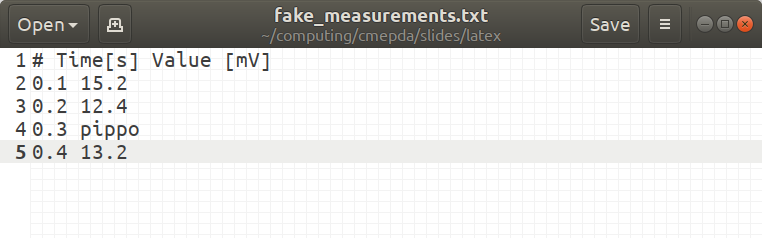
\includegraphics[width=0.8\textwidth]{lab_file.png}
\end{figure}

\input{pygments/when_to_catch}

\hrulefill

\subsubsection{Catch too early}
\input{pygments/when_to_catch_1}

\hrulefill

\subsubsection{Catch when needed}
\input{pygments/when_to_catch_2}

\newpage 
\section{Generators}

\subsection{Iterators and iterables}
Let's analyse the properties of iterables a little deeper. Here's a little reminder of what we already know:
\begin{itemize}
    \item An \textbf{iterable} in Python is something that has a \texttt{\_\_iter\_\_} method, which returns an \textit{iterator}
    \item An \textbf{iterator} is an object that implements a \texttt{\_\_next\_\_} method which is used to retrieve elements one at a time
\end{itemize}
Here's more information about iterators:
\begin{itemize}
    \item When there are no more elements to return, the iterator signals that with a specific exception: \texttt{StopIteration()}
    \item An iterator also implements a \texttt{\_\_iter\_\_} method that returns itself. So an iterator is also technically an iterable\footnote{Only technically because an iterator has no data of its own, so you always need a "real" iterable to actually iterate}, but the opposite is not true.
\end{itemize}
Take a look at the following example where we loop over all the elements of a list (iterable) using \texttt{for} and \texttt{while}:

\input{pygments/show_iterator}

In the following examples we implemented two iterators of our own and tested their behaviour. Look at their structure and try and write one of your own:

\textbf{- A simple iterator}
\input{pygments/simple_iterator}
\hrulefill
\input{pygments/test_simple_iterator}

\bigskip

\textbf{- A crazy iterator}
\input{pygments/crazy_iterator}
\hrulefill
\input{pygments/test_crazy_iterator}

\subsection{Generators}

We have seen that iterators are useful to iterate over container. However that assumes a containers exists which means slots of memory are being used.
\textbf{Generators} allow you to loop over sequences of items even when they don't exist before - the items are just created \textbf{lazily} the moment they are required. For example you can write a generator to loop over the Fibonacci succession. You can't create the sequence earlier, since it is not finite!

Generators are created through either \textit{generator expressions} or \textit{generator functions}. In real life most of the time you will simply use pre-made functions that return a generator, like \texttt{range()} (in Python 3). Generators can be used to iterate in for loops, just like iterators. Take a look at these simple generator expressions:

\input{pygments/generators}

A \textbf{generator function} is a function that contains the keyword \texttt{yield} at least once in his body. When you call a generator function the code is not executed - instead a generator object is created and returned (even if you don't have a return statement). Each call to \texttt{next()} on the returned generator will make the function code run until it finds a \texttt{yield} statement. Then the execution is paused and the value of the expression on the right of \texttt{yield} is returned (yielded) to the caller. A further call of next will resume the execution from where it was suspended until the next \texttt{yield} and so on. Eventually, when the function body ends, \texttt{StopIteration} is raised. Usually generators functions contain a loop, but it's not mandatory!
Here's two examples of generator functions:

\textbf{- Simple generator function}
\input{pygments/generator_functions}

\textbf{- Infinite sequence generators}
\input{pygments/fibonacci}

Take a look at the list of functions in Sec. \ref{sec:special_iterable}: Many of those return a generator from an iterable, such as: \texttt{enumerate}, \texttt{map}, \texttt{filter}, \texttt{zip}, \texttt{reversed} and all the functions mentioned from the \texttt{itertools} library. Look at the documentation of each function if you want to see how to properly call it. In this next example we will showcase the capabilities of \texttt{itertools}:

\input{pygments/itertools_showcase}

\hrulefill
\subsubsection{Note: Lambda functions}

\textbf{Anonymous functions}, or \textbf{lambda functions}, are a construct typical of \textbf{functional programming} (see for example \url{https://en.wikipedia.org/wiki/Lambda_calculus} and \url{https://en.wikipedia.org/wiki/Functional_programming}).

In Python a lambda function is essentially a special syntax for creating a function on the fly, without giving it a name. They are limited to \textit{a single expression}, which is returned to the user. Many of the typical uses for lambdas are already covered in Python by generator expressions and comprehension, so this is more like a niche feature of the language. Here's an example:

\input{pygments/lambda}
\hrulefill

This next example simulates a programming session in which the user tries to create a more complex iterator, simplifying its structure step by step:

\textbf{- Recap example: file iterator}
\input{pygments/file_iterator}
\bigskip

\textbf{- File iterator redone}
\input{pygments/file_iterator_2}
\bigskip

\textbf{- File iterator, final version}
\input{pygments/file_iterator_3}
\section{Advanced features of functions and decorators}

\subsection{Functions inside functions}
Functions in python are \textbf{first class object}. The name is a bit misleading, but what it actually means is that functions can be passed as arguments to other functions and returned as result from other functions. This shouldn't surprise you much: functions are objects of a \texttt{function} class, so they behave like any other variable in Python. Another thing you can (and sometimes want to) do is \textit{defining} a function inside another. Let's see how it works:

\input{pygments/inner_outer}

\subsection{Closures and free variables}
When a function is created inside another function it has access to the local variables of the outer function, even after its scope ended. This is technically possible because those variables are kept in a special space of memory, the \textbf{closure} of the inner function. Such variables are called \textbf{free variables}. In this way, a function can maintain a \textbf{state} within its closure. This makes possible the use of functions for tasks that in other languages are reserved to classes. Let's take a look at the following example. Here the function \texttt{rotate} is obviously inefficient, while \texttt{efficient\_rotate} requires the user to do most of the work:

\input{pygments/rotation_naive}

Here's the best way to do it thanks to free variables:

\input{pygments/rotator}

Pay attention when using free variables: if you \textit{assign} a free variable in the inner function, by default a new, local variable is created instead! To avoid this, you have to explicitly declare that you want to access the variable in the closure using the \textbf{nonlocal} keyword. Remember: \textit{"Explicit is better then implicit"}, The Zen of Python.
Here's a wrongfully written code... 

\input{pygments/closure_wrong}

\bigskip

...and here's how you should actually do it:

\bigskip

\input{pygments/closure_right}

\subsection{Wrapping functions}
The typical use of defining a function inside a function is to create a \textbf{wrapper}. A wrapper is a function that calls another one adding a layer of functionalities in between. For example it may do some pre-process of the input, or change the output in some way, or measure the execution time or whatever we want.

The technique for creating a wrapper function in Python is:
\begin{enumerate}
    \item Pass the function that we want to wrap as argument of the outer function.
    \item Inside the outer function we define an inner function, which is the actual wrapper.
    \item The wrapper calls the wrapped function and adds its functionalities, before and/or after the call. It may return the same output or a manipulated one.
    \item From the outer function we return the wrapper.
\end{enumerate}
Take a look at the following example:

\input{pygments/wrapper}

\subsection{Decorators}
Often, when you wrap a function, you don't want to change it's name, so you reassign the wrapped function to its old name. In fact, this technique is so common that python introduced a special syntax for it: \textbf{decorators}. A decorated function has simply the name of the wrapper added with a \texttt{@} on top of its declaration. Here's an example:


\input{pygments/decorator}
\hrulefill
\input{pygments/time_measuring_decor}

Now, let's review some of the most common decorators:

\subsubsection{- The \texttt{@classmethod} decorator}
We have already seen a built-in Python decorator: \texttt{@property}. We used that to get proper encapsulation. There is another built-in decorator which is very useful for classes: \texttt{@classmethod}. A \textbf{classmethod} is like a class attribute: you don't need an instance to use it. A class method can access class attributes but not instance attributes. The main use for class methods is to provide \textbf{alternate constructors}.

\input{pygments/classmethod}

\subsubsection{- The \texttt{@staticmethod} decorator}
Another built-in decorator (though less used than \texttt{@classmethod}) is \texttt{@staticmethod}. A static method is a method that does not receive the class or instance as first argument. Because of that, a static method does not alter the state of the class. In some sense a static method is only loosely coupled to the class - it is defined inside the class body just for convenience (maybe for semantic proximity) but it could be defined outside the class as well.

\input{pygments/staticmethod}

\subsubsection{- The \texttt{@dataclass} decorator}
Another useful decorator is \texttt{@dataclass}. A \textbf{dataclass} is a class that is designed to only (or mostly) hold data values. A dataclass is defined by declaring the name and type of its attributes. You do not have to type any other code, the interpreter will automatically generate the \texttt{\_\_init\_\_}, \texttt{\_\_eq\_\_} and \texttt{\_\_repr\_\_} special methods for you.

\input{pygments/dataclass}

\subsection{Passing arguments to a decorator}
Making a decorator that accepts arguments is somewhat more complex. The basic idea is that you need to add yet another level: a \textbf{decorator factory function}.

So you now end up with three levels:
\begin{enumerate}
    \item The decorator factory that takes the parameters for the decorators, creates it and returns it;
    \item The decorator that takes as input a function and returns the wrapper;
    \item The wrapper that implements the actual additional functionalities; usually takes as input the same parameters as the decorated/wrapped function and returns its results, if any.
\end{enumerate}
Take a look at this four more complex examples to become a master of decorators:

\textbf{- Example 1: Decorception}
\input{pygments/decorator_factory}

\textbf{- Example 2: Repeat}
\input{pygments/decorator_repeat}

\textbf{- Example 3: Customizing dataclass methods}
\input{pygments/dataclass_customized}

\textbf{- Example 4: Chaining decorators}
\input{pygments/decorator_chain}
\section{Basic optimization}

\subsection{The correct workflow for optimization}
\textbf{Optimization} is the process of making your code more performant. \textbf{Profiling} is the study of the resource cost of your code (CPU, RAM, hard disk, network, etc\dots) possibly as a function of time, input, or execution status.

Always remember this: \textbf{Premature optimization is the root of all evil!}

You must always follow this workflow:
\begin{enumerate}
    \item Write correct, readable, debugged, tested, documented code \underline{ignoring performance completely}.
    \item If the performance is good: great, you are done!
    \item If the performance is not good: \textit{profile} to find the bottlenecks.
    \item Start \textit{optimization} from the problematic lines. Everything else is a waste of time.
    \item Keep testing whenever you have a new version!
\end{enumerate}

\subsection{Basic CPU memory structure}
Data is processed by CPUs (or GPUs). CPUs have a small memory called \textit{cache} (or multiple levels of them: L1, L2, etc\dots) of a few KB from which they get the data. Generally, L1 is on the processor and L2 or L3 are shared among different processors, but this scheme may vary. The connection between the CPU and the cache is called the \textit{backside bus} and is very fast. Your data needs to be transferred from the RAM to the cache, which happens through the \textit{frontside bus}, which is slower than the backside bus. Sometimes you need to retrieve data from the hard disk or the network: in that case the time required to retrieve the data is often significantly larger. This is of course a very naive description of the structure of a PC, but you should keep it in mind while you try to optimize your code.

\subsection{General optimization goals}
As obvious as it is, what usually matters the most for optimization is doing fewer operations! Use an optimal algorithm for your job. Reduce as much as possible the slow operations involving hard drives and networks.

Also, make sure that the next data required by the CPU is already in the cache, and need not be retrieved from the RAM through the slower frontside bus. 

If possible, use \textit{vectorization}; that is, let the CPU do multiple operations at once. If the system has more than one processor, as most computers do nowadays, try to \textit{parallelize} the work across multiple cores (this will be covered in the next lessons). 

Python is a high-level language and generally does not allow direct control over memory usage or the cache. However, there are ways to improve the speed of the code, as we will see!

\subsection{What slows down your code?}
The CPU uses algorithms for \emph{branch prediction} and \emph{pipelining} in order to try to load the next instructions (and the required data) while processing the current one. Whenever that fails, you will get \emph{branch misses} and/or \emph{cache misses}, plus usually a number of \emph{stalled cycles} on the frontside or backside bus. Using data structures that keep data contiguously in memory is better, as sparse data is more difficult to move into the cache with a single transfer. That's why a list is worse than an array or a \texttt{numpy} array for numerical operations. 

\emph{Context switches} and \emph{CPU migrations} are managed by the OS, so there is not much you can do about that. Memory allocations are also expensive, as the program is paused and waits for the OS to find a free memory location. This, together with I/O operations, is a typical case where a context switch may happen.
%\end{comment}

% -------------------------------------------------------------------
% PART III: PARALLEL PROGRAMMING
% -------------------------------------------------------------------
\chapter[Parallel computing]{Parallel computing \\[0.5ex] \large \textit{(Prof. Lamanna)}}

%\begin{comment}
\section{Computer architecture from a performance point of view: from serial to parallel} 


The goal of this section is to introduce key concepts of computer architecture in order to: 
\begin{itemize}
    \item[-] Identify the characteristics of the processors that most influence the computing performance;
    \item[-] Identify the limits of the standard architecture (Dennard and Moore scaling, Flynn's taxonomy);
    \item[-] Introduce concurrency and parallelism and study their limits (Amdahl and Gustafson laws).
\end{itemize} 

\subsection{Von Neumann architecture}
The so-called \textbf{Von Neumann architecture} was introduced in 1945 by John von Neumann and is based on the \textit{Universal Turing Machine} (UTM) by Alan Turing (1936). It consists of 5 main elements:

\begin{center}
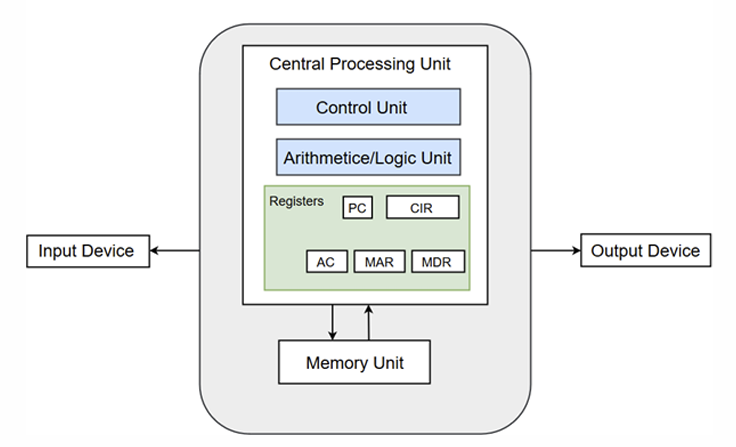
\includegraphics[width=0.6\textwidth]{figuresP/lesson_parallel_1_pag_6.png}
\end{center}

\begin{itemize}
    \item \textbf{Central Processing Unit} (CPU) composed of:
    \begin{itemize}
    \item \textbf{Arithmetic and Logic Unit (ALU)}: performs all arithmetic calculations and logical operations required to execute instructions.
    \item \textbf{Control Unit}: decodes instructions fetched from memory and orchestrates the operation of the entire system by sending timing and control signals.
    \end{itemize}
    \item \textbf{Memory}: a shared storage area that holds both the program's instructions and the data currently being processed. The so-called \textbf{Random Access Memory (RAM)} is the \textit{primary memory}. It is volatile (data is lost when power is cut) and it is the one that actually stores the instructions and data of currently running processes. The \textbf{Secondary Storage (SSD/HDD)} commonly referred to as "disk space,"  is the \textit{non-volatile} storage. It is designed for long-term data retention. While significantly slower than RAM, it offers much larger capacities at a lower cost. Finally, the CPU itself has local, fast-read memory units called \textbf{registers}. 
    \item \textbf{Bus}: communication system composed of physical wires that transfers addresses, data, and signals between the CPU, memory, and peripherals.
    \item \textbf{I/O (Input/Output)}: interfaces that allow the computer to interact with the external world, receiving data from users and providing the results of computations.
\end{itemize}

The so-called \textbf{Von Neumann bottleneck} refers to the throughput limitation between the CPU and memory, which occurs because the shared bus cannot fetch instructions and data simultaneously. To mitigate this phenomenon and improve performance, several hardware strategies are employed:
\begin{itemize}
    \item \textbf{Caching and Memory Hierarchy}: Small, high-speed memory units (L1, L2, L3 \textbf{caches}) are placed directly on the CPU chip to store frequently used data and instructions, drastically reducing the number of slow accesses to the main RAM. A multilevel cache represents a good trade-off between hit-rate and latency. For example the \textbf{I-Cache} and \textbf{D-Cache} are L1 caches dedicated respectively to instructions and data to avoid access conflicts at the core level. The hierarchy of both data access and instruction fetching is fundamental in present computer architecture.
    \begin{center}
        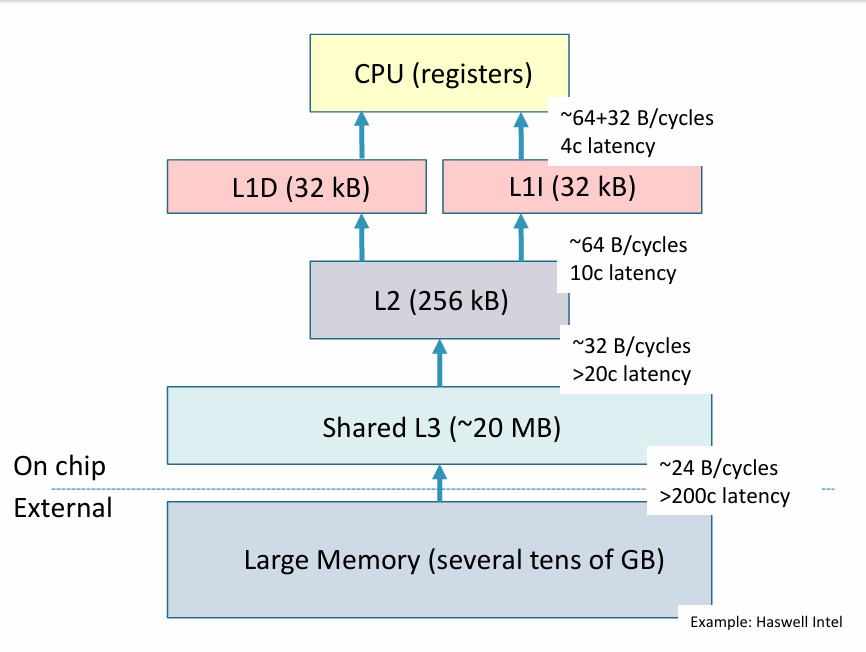
\includegraphics[width=0.6\textwidth]{figuresP/lesson_parallel_1_pag_9.png}   
    \end{center}
    \item \textbf{Harvard Architecture}: By providing separate physical pathways and storage for instructions and data, the processor can perform an instruction fetch and a data access at the same time, effectively doubling the available bandwidth (see representation below).
    \begin{center}
        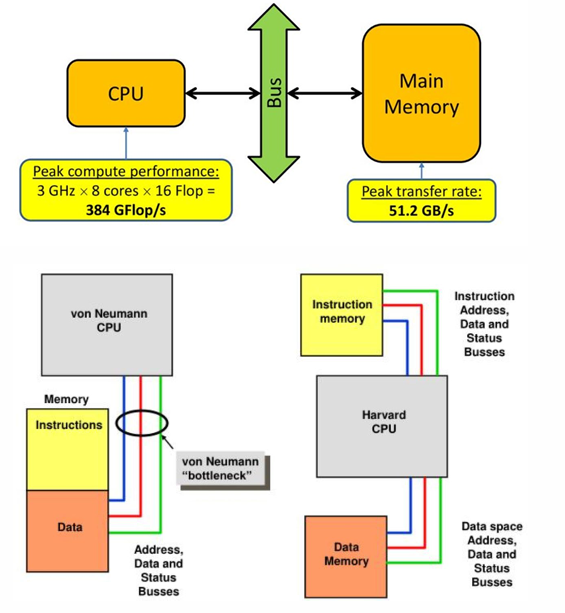
\includegraphics[width=0.4\textwidth]{figuresP/lesson_parallel_1_pag_7.png}
    \end{center}
    \item \textbf{Branch Prediction}: A sophisticated technique where the CPU "guesses" the outcome of conditional statements (e.g., \texttt{if} blocks) to pre-fetch and begin executing the most likely next instructions, preventing the pipeline from stalling (see below).
\end{itemize}

\hrulefill

\subsubsection{Note: simple server architecture}

A \textbf{server} is a specialized computer system or a software process designed to provide services, data, or resources to other programs or devices, known as \textbf{clients}, over a network. This interaction follows the \textbf{client-server model}, where the server "listens" for incoming requests and responds by processing the required task or delivering the requested information.

From a hardware perspective, servers are typically high-performance machines engineered for reliability and availability, often operating 24/7. From a software perspective, a server is a program (such as a web server or a database server) that manages access to a centralized resource. \footnote{The previous definition of a server was surely NOT given by ChatGPT}.

In a modern server, several components interact to execute programs efficiently:
\begin{itemize}
    \item[-] \textit{Processors/Cores}: Processing units that execute instructions, often organized in multi-core layouts for parallel computation.
    \item[-] \textit{Shared Caches (L3)}: A larger memory pool shared among all cores to synchronize data and minimize slow accesses to the main RAM.
    \item[-] \textit{Memory Controllers}: Logic circuits that manage the high-speed data flow between the processor and the system memory.
    \item[-] \textit{I/O Subsystems}: The infrastructure (e.g., PCIe) connecting the CPU to storage, network, and external peripherals.
\end{itemize}
For example \textit{NUMA (Non-Uniform Memory Access)} is a multi-socket architecture where memory access latency depends on the physical distance between the processor and the memory bank.

\begin{center}
    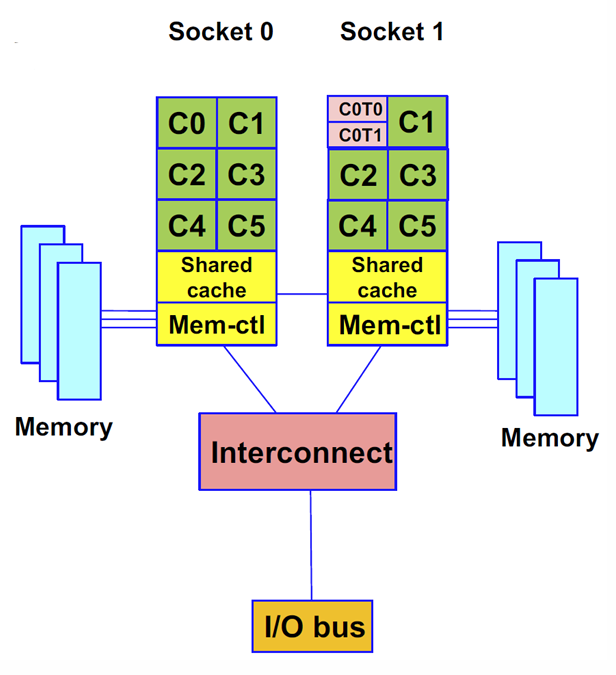
\includegraphics[width=0.4\textwidth]{figuresP/lesson_parallel_1_pag_8.png}
\end{center}

\hrulefill

\subsection{Parallelism and the seven dimensions of performance}
The modern PC performance depends on (at least) seven characteristics:
\begin{itemize}
    \item[-] Data and Instruction level:
    \begin{itemize}
        \item[1] Hardware vectors
        \item[2] Superscalars
        \item[3] Pipelining
    \end{itemize}
    \item[-] Task level:
    \begin{itemize}
        \item[4] Hardware multithreading
        \item[5] Multiple cores
        \item[6] Multiple sockets
    \end{itemize}
    \item[-] Application level: 
    \begin{itemize}
        \item[7] Multiple nodes
    \end{itemize}
\end{itemize}
Obviously, our goal is to maximize the performance of our PC, which means reducing the execution time of our program. In other words, we want to complete a certain task in the least possible amount of clock cycles. The best way to do it is \textit{parallelism}.

\textbf{Parallelism} is the simultaneous execution of multiple computations. While often associated with multi-core processors, parallelism actually occurs at different "dimensions", matching the "levels" listed above. 

It starts at the micro level with \textbf{Instruction Level Parallelism (ILP)}, where a single core overlaps the execution of machine instructions. It scales up to \textbf{Task Level Parallelism (TLP)}, where distinct \textit{threads} or processes run on separate physical cores or processors. Remember this definition: a \textbf{thread} is the smallest instruction set that can be managed independently by a scheduler (typically in the operating system). Finally, it reaches the \textbf{Application Level}, where workloads are distributed across entirely different machines (nodes).

We will now dive a little deeper into the first 3 points of the "performance list", but the next 4 will be the central core of this part of the course. 

\hrulefill

\subsubsection{Note: Clock Cycles}
A \textbf{clock cycle} is the fundamental unit of time for a processor, acting as an electronic "heartbeat" that synchronizes internal operations. The \textit{clock rate} (frequency), measured in Gigahertz (GHz), defines how many billions of cycles occur per second. While a higher frequency generally speeds up execution by shortening the interval between processing steps, the actual performance also depends on the \textit{CPI} (Cycles Per Instruction). Since different instructions require a varying number of cycles to complete, true execution speed is a trade-off between how fast the clock "ticks" and how efficiently instructions are retired during each cycle.

\hrulefill

\subsection{Instruction level parallelism}
\subsubsection{[1] Vector processors}
Modern processors incorporate specialized hardware and wide registers (such as XMM and YMM) to support hardware-level \textbf{vectorization} through instruction sets like \textbf{SSE/SSE2} and \textbf{AVX}. You probably don't know what these are, but just remember that when you work with \texttt{numpy} arrays you are exploiting them without even knowing it. With these components, one can obtain a \textit{SIMD (Single Instruction Multiple Data)} architecture (one operation produces multiple results, e.g. a sum of two vectors of 4 floating point elements is a single instruction that produces 4 results) even in a single core. We will get to this concept in a second. \\
Vectorization at the instruction level is the first simple example of parallelism. 

\begin{center}
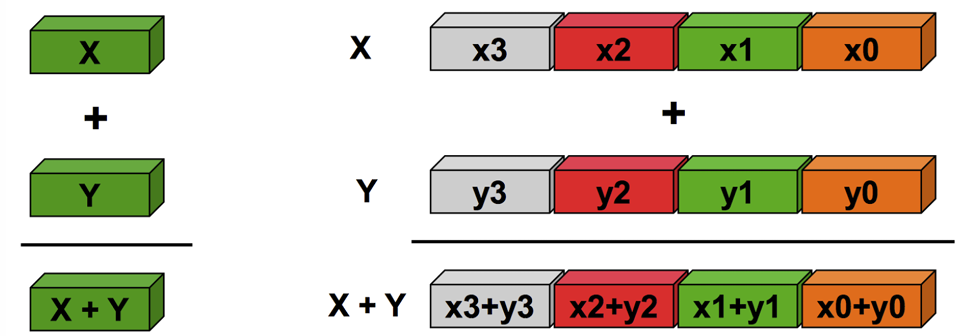
\includegraphics[width=0.4\textwidth]{figuresP/lesson_parallel_1_pag_11.png}
\end{center}

\subsubsection{[2] Superscalars}
A \textbf{superscalar} architecture is in between pure scalar and pure vector. In the CPU there can be several hardware units called \textbf{Functional Units (FU)} that can execute different operations on different data at the same time and can be "specialized" for certain tasks. A \textit{decoder} "reads" the incoming instruction stream and passes it to the \textit{dispatcher}, which assigns the correct task to each FU. The decoder and the dispatcher must have the capability to manage two instructions in one clock cycle. 

A superscalar processor is useful for \textbf{branch prediction}. To understand this concept, just think about an \texttt{if - else} statement that depends on a certain \texttt{condition}. Before executing one of the two branches of the statement, the CPU must know if \texttt{condition} is \texttt{True} (in which case it will execute the \texttt{if} branch) or \texttt{False} (in which case it will execute the \texttt{else} branch). However, in a superscalar processor two different FUs can simultaneously execute the two branches and then the CPU will choose which one to use once \texttt{condition} is defined. That's a simple example of branch prediction.

\begin{center}
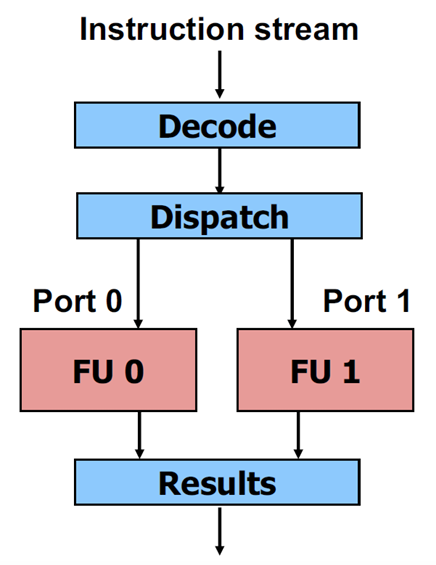
\includegraphics[width=0.3\textwidth]{figuresP/lesson_parallel_1_pag_12.png}
\end{center}

\subsubsection{[3] Pipelining}
What steps does the processor follow to execute an instruction? Here they are:
\begin{itemize}
    \item[-] \underline{Instruction fetching (IF)}: the instructions to execute and the necessary data are fetched from the memory (RAM or cache) thanks to the PC;
    \item[-] \underline{Instruction Decode (ID)}: the processor interprets the instruction and reads the data from the registers;
    \item[-] \underline{Execution (EX)}: the ALU executes the instructions;
    \item[-] \underline{Memory Access (MEM}, done only if the instruction requires to load or store something in the memory);
    \item[-] \underline{Write Back (WB)}: the result is written in a register.
\end{itemize}

Integer and logic instructions have a determined latency, i.e. a fixed number of clock cycles needed for the EX phase. Here are some examples \footnote{You can easily find what these three-letter formulas mean online. "ADD" stands for "addition" (the sum between two integers); "IMUL" is the sum of two floating point numbers etc\dots}: 
\begin{itemize}
    \item[-] 1 cycle: ADD, AND, SHL, ROR, FABS
    \item[-] 3 cycles: IMUL, FADD
    \item[-] 5 cycles: FMUL
    \item[-] 13-23 cycles: IDEV
    \item[-] 27 cycles: FSQRT
\end{itemize} 

\textbf{Pipelining} is the capability to execute different stages of consecutive instructions at the same time. 

Look at the following scheme which represents a pipeline of\textit{ depth 3} (as it "contains" 3 simple operations with 1 cycle for the EX phase): squares vertically aligned contain stages of different instructions that can be executed in the same clock cycle.

Without the pipeline (15 clock cycles of latency):
\begin{center}
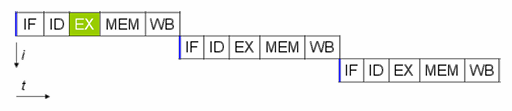
\includegraphics[width=0.7\textwidth]{figuresP/lesson_parallel_1_pag_13.png}
\end{center}

With the pipeline (7 clock cycles of latency):
\begin{center}
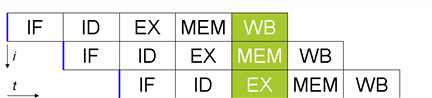
\includegraphics[width=0.6\textwidth]{figuresP/lesson_parallel_1_pag_13a.png}
\end{center}

Here's a more realistic example:
\begin{center}
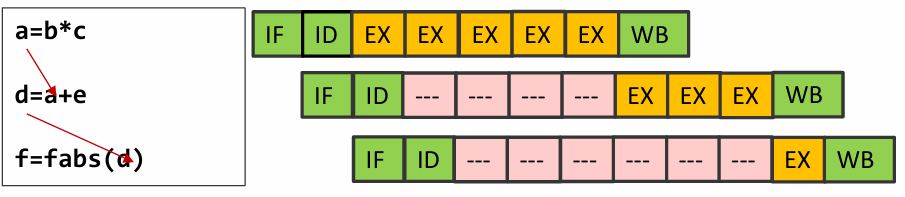
\includegraphics[width=0.9\textwidth]{figuresP/lesson_parallel_1_pag_13b.png}
\end{center}

\subsubsection{Recap and conclusions}
As we've seen, superscalars, pipelining and vectorization are methods to exploit some parallelism at the instruction and data level. Probably \textit{OOO (Out-of-order) execution} should be included in this category, but we won't discuss it here. 

The possible performance improvement thanks to ILP depends on the problem and data structures and can result in $1\times-10\times$ speed-up for superscalars and pipelines and in $2\times, 4\times, 8\times, 16\times$ speed-up for vectorization.

However, these methods will incur in \textit{saturation} because they are limited by the available CPU resources. Here are some examples:
\begin{itemize}
    \item[-] Pentium 4: 30 pipeline stages (nowadays 10-15 maximum), maximum number of pipelines in a processor (2000s).
    \item[-] ARM A57 (Apple A7/A8): 9 ports, 6 instructions superscalar
    \item[-] Intel Tiger Lake: vector of 512 bits for a subset of AVX512 instructions
\end{itemize}
The point is: \textbf{can CPU resources grow indefinitely?}

\subsection{Dennard scaling}

You might think that to enhance performance one could just maximize the clock rate. Nowadays there exist oscillators that can reach a frequency in the order of the THz, so it seems that the speed-up problem just depends on technical innovation towards faster oscillators. However, there's a fallacy in this kind of reasoning.

As you know from the \textit{Digital Technologies} course, modern digital CPUs are based on \textbf{transistors} (like the one represented below), which can be used as switches\footnote{If you want to easily understand how a CPU works thanks to transistors, take a look at this playlist \url{https://youtube.com/playlist?list=PL9vTTBa7QaQOoMfpP3ztvgyQkPWDPfJez&si=i0Yy-61cQFOv8zpt}, and in particular at this video \url{https://youtu.be/HjneAhCy2N4?si=LX_gNx31aW7GgXWl}}. The time needed to switch from a state to the other depends on the gate length $L$. 

\begin{center}
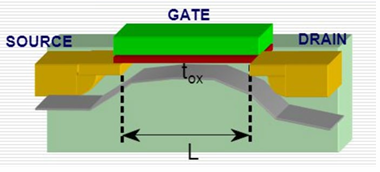
\includegraphics[width=0.45\textwidth]{figuresP/lesson_parallel_1_pag_15.png}
\end{center}

If we are looking for a faster clock cycle, we are then going to need smaller and smaller transistors. In other words, we need more \textbf{integration}, which means that there should be a greater number of components on the same chip surface. In particular the number of transistors that can be integrated on a chip will scale proportionally to $L^2$. However, a larger number of components means a greater consumption of energy to switch the transistors. Is there an energy problem, then? Not really, because the voltage $V$ and the current intensity $i$ needed to switch the transistors scale proportionally to $L$. Since power consumption is equal to $V \cdot i$, the two effects should cancel out. 

The continuous decrease in transistor dimensions ( $\equiv$ increasing integration) is referred to as \textbf{Dennard Scaling} (from an article by Dennard et al. in 1974 in the IEEE Journal of Solid State Circuits). You can find a schematic representation below.

\begin{center}
    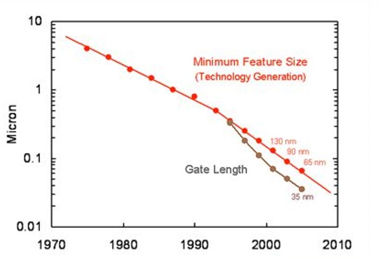
\includegraphics[width=0.49\textwidth]{figuresP/lesson_parallel_1_pag_15a.png}
    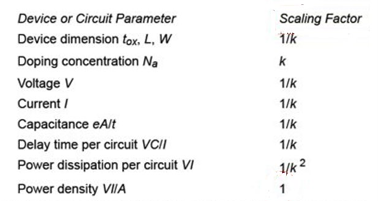
\includegraphics[width=0.49\textwidth]{figuresP/lesson_parallel_1_pag_15b.png}
\end{center}

So\dots what's the matter? With very high integration \textit{it is not true anymore that the power consumption is the same, due to an increase in current leakage}: in smaller transistors you will need more power to compensate for the \textit{inverse currents}. Also, the switching characteristics of a transistor depend on it's temperature, which will rapidly increase in very crowded chips. That means that Dennard scaling cannot continue indefinitely, but processors have a power limit due to heat (even with better packaging and cooling systems).  

\subsection{Moore scaling}
\textbf{Moore's "law"} is the empirical observation that the mean number of transistors per chip doubles about each two years, while the performance of CPU doubles each 18 months. Take a look at the graphs below. \\
Moore's prediction was verified for decades but around 2005 it started to show saturation. That is of course closely related to Dennard scaling. In the first years of the 2000s, people realized that increasing the clock frequency and integrating was not the best way (anymore) to increase the processor performance.

\begin{figure}[H]
    \centering
    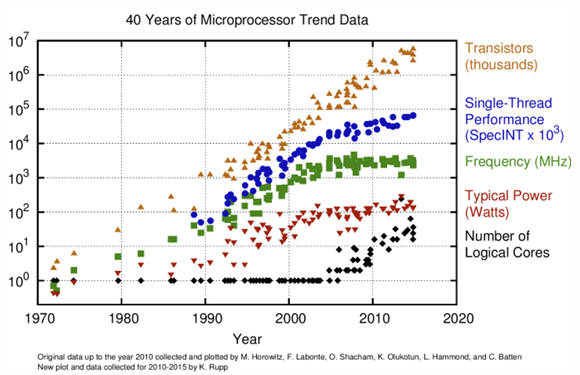
\includegraphics[width=0.49\textwidth]{figuresP/lesson_parallel_1_pag_16a.png}
    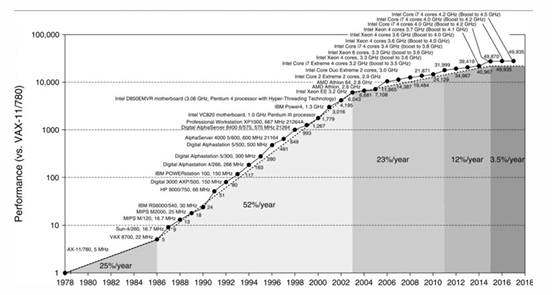
\includegraphics[width=0.49\textwidth]{figuresP/lesson_parallel_1_pag_16b.png}
\end{figure}

\subsection{Task level parallelism}

How to avoid saturation? Instruction level parallelism achieved significant performance advantages. Getting better at ILP is still possible, but the complexity of CPU is more than linear. We need a next level in parallelism: \textbf{Task Level Parallelism (TLP)}. We want our series of \textbf{instruction streams (threads) to be executed by more than one processor at once}, while at the instruction level we were talking about having a \textit{single} processor doing our work in a smarter (parallel) way. 

Let's start by introducing the so-called \textbf{Flynn's taxonomy}, which is a classification of computer architectures based on the number of data streams and instructions streams. It consists of 4 categories:
\begin{itemize}
    \item[-] Single Instruction Single Data (SISD)
    \item[-] Single Instruction Multiple Data (SIMD)
    \item[-] Multiple Instructions Single Data (MISD)
    \item[-] Multiple Instructions Multiple Data (MIMD)
\end{itemize}
Let's take a look at each of them.

In a \textbf{Single Instruction Single Data} architecture, only one instruction operates for each time slot on one data. That's the familiar sequential processing.

Example: The operations \texttt{a+b}, \texttt{c+d}, \texttt{e+f}, \texttt{g+h} will be executed one after the other.

\begin{center}
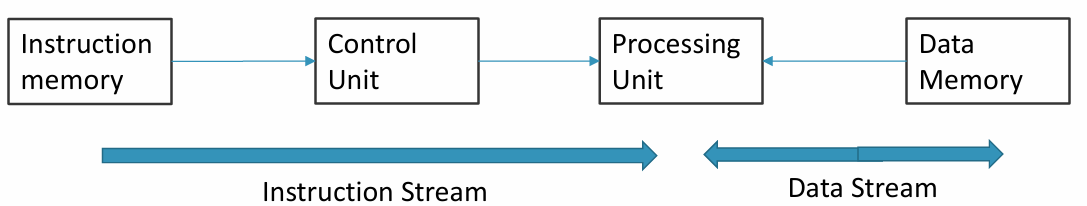
\includegraphics[width=0.7\textwidth]{figuresP/lesson_parallel_1_pag_19.png}
\end{center}

In a \textbf{Single Instruction Multiple Data} architecture, one instruction can operate on multiple data at once. Modern processors implement SIMD via vector registers, as seen in the ILP section.

Example: The operations \texttt{a+b}, \texttt{c+d}, \texttt{e+f}, \texttt{g+h} can be executed together, since it's the same instruction (the addition) that is executed on different variables. That corresponds to a vector sum.

\begin{center}
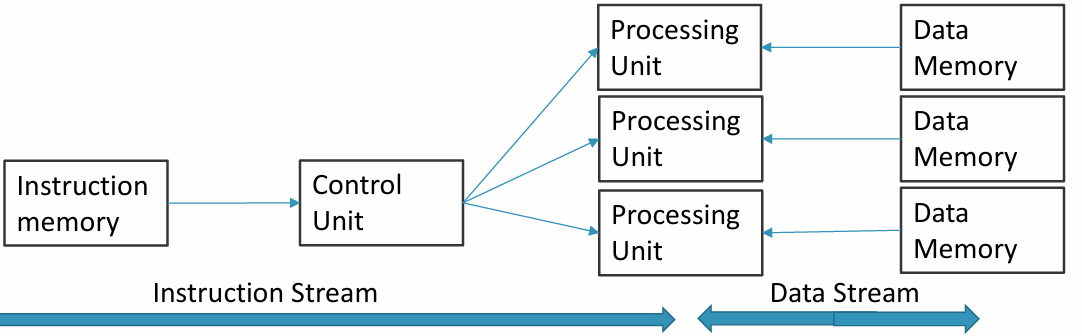
\includegraphics[width=0.7\textwidth]{figuresP/lesson_parallel_1_pag_20.png}
\end{center}

In a \textbf{Multiple Instruction Multiple Data} architecture, multiple instruction streams can operate on multiple data streams. Most supercomputers are organized as MIMD architectures including multi-core superscalar processors, multi-processor systems, and distributed systems.

Example: The operations \texttt{a+b}, \texttt{c+d}, \texttt{e*f}, \texttt{g*h} can be executed together, even if they consist of two instructions (addition and multiplication) that are executed on different variables.

\begin{center}
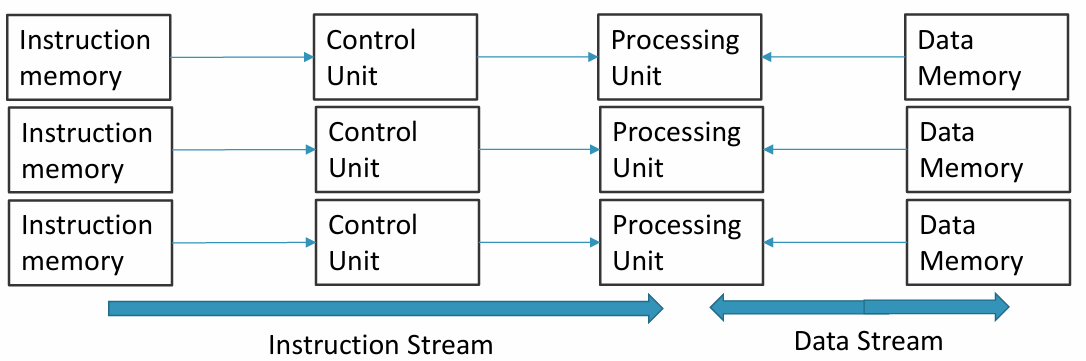
\includegraphics[width=0.7\textwidth]{figuresP/lesson_parallel_1_pag_21.png}
\end{center}

In a \textbf{Multiple Instruction Single Data} architecture, multiple instruction streams can operate on a single data stream. It is not commonly seen for computing. Sometimes the so-called \textit{systolic array} is seen as MISD (we won't treat it here). Usually, this is an architecture used for fault tolerance (processing a certain data more than once to be sure of the result), like in some pacemakers. 

\begin{center}
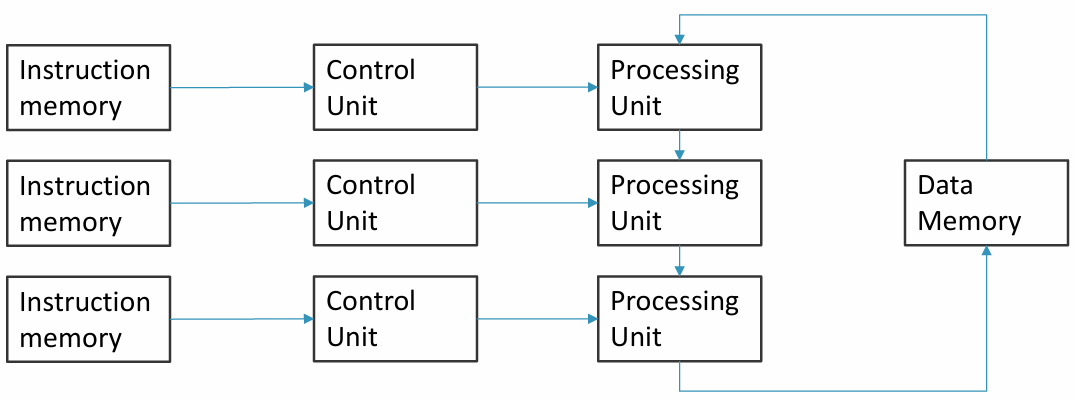
\includegraphics[width=0.7\textwidth]{figuresP/lesson_parallel_1_pag_22.png}
\end{center}

\subsection{Multiprocessors}
The standard for modern high-performance computing is the \textbf{Multiprocessor} system, an implementation of the MIMD architecture. Unlike SIMD, where a single controller drives multiple ALUs, here each processor is fully independent (it has its own PC) and communicates via \textbf{shared memory}.

We can utilize a multiprocessor system for two main goals:
\begin{itemize}
    \item \textbf{Job-level parallelism}: Running independent processes on different processors to increase throughput (e.g., browser on Core 1, compiler on Core 2). No program modification is needed.
    \item \textbf{Parallel processing}: Using multiple processors to speed up a \textit{single} program. This requires the program to be explicitly designed for parallelism using multiple cooperating threads.
\end{itemize}

To implement parallel processing, the programmer must decompose the problem into parts that can run simultaneously. There are two main approaches:

\begin{itemize}
    \item \textbf{Domain Decomposition}: The \textit{data} is divided into chunks, and parallel tasks perform the same operation on different data segments. \\
    Example: An image processing tool where the image is sliced into 4 parts, and 4 processors apply the same filter to their respective slice simultaneously. Ideally suited for both SIMD units and MIMD architectures.
    \begin{center}
    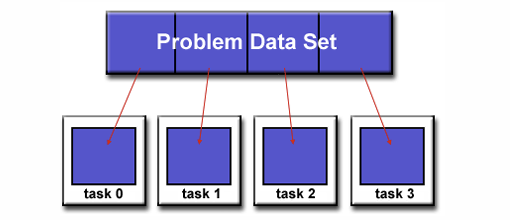
\includegraphics[width=0.38\textwidth]{figuresP/lesson_parallel_1_pag_23.png}
    \end{center}
    \item \textbf{Functional Decomposition}: The program is divided into distinct functions or tasks.\\
    Example: In a video editor, one thread handles the UI, another decodes audio, and a third renders the video preview. MIMD architectures are required here, as the processors must execute different instructions streams.
    \begin{center}
    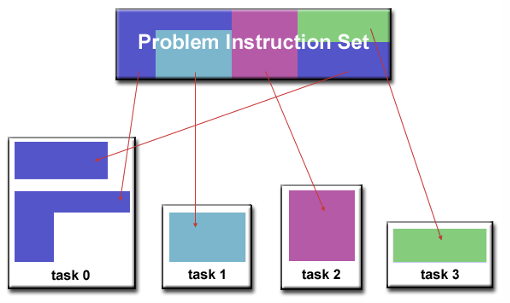
\includegraphics[width=0.38\textwidth]{figuresP/lesson_parallel_1_pag_23a.png}
    \end{center}
\end{itemize}

Now that you know what task level parallelism is, let's talk about another way to execute multiple programs: \textit{concurrency}.

\subsection{Concurrency}

As said, in a sequential processing one step follows another in sequence, and one processor is all that is needed to run the algorithm. To be more technical, you can say that each \textit{thread} of the program is executed one after the other.

Knowing what we said in this section, we expect that a computer with a single processing unit cannot do better than sequential processing. However, you might have used a single-core computer and been able to open a browser while listening to some music, for example. How is that possible? That's a first example of what is called \textbf{Concurrent Processing}.

\textbf{Concurrency} is a property of the system where multiple tasks are logically "in progress" at the same time. But wait, isn't this the definition of parallelism? Not really, we will get to it in a second.\\
There are 4 main types of concurrent processing implementation: (the first one should start to clarify the difference between parallelism and concurrency):

\subsubsection{- Multiprogramming (Time-sharing)}
In a \textbf{multiprogramming} context, a single CPU is shared among many users or programs, thanks to a time-shared algorithm or a priority algorithm. How is it possible? The CPU gives the illusion of simultaneous processing by interleaving threads with a series of \textbf{context switches}. For example, it will execute a certain thread A until a certain latency has to happen (e.g. waiting for an I/O), then with a context switch it may start to work on thread B and so on until all the tasks are executed. That's why you can listen to Gangnam Style while searching for "Best 10 moments of respect in sports" on Google in a single-core computer: you are not really running the two programs together, you are constantly switching between one and the other several times per second. 

\begin{center}
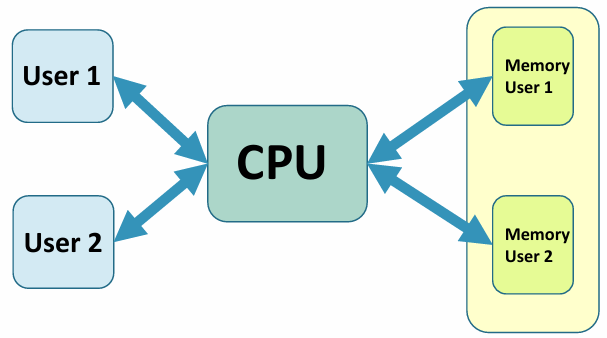
\includegraphics[width=0.4\textwidth]{figuresP/lesson_parallel_1_pag_28.png}
\end{center}

\subsubsection{- Multiprocessing (Hardware Parallelism)}
If one or more users execute multiple tasks at the same time while using multiple cores in a multiprocessor, it is referred to as \textbf{multiprocessing}. Of course this doesn't mean that every single processor can't also timeshare among several tasks. Remember that in this case the memory is shared between the cores. 

\begin{center}
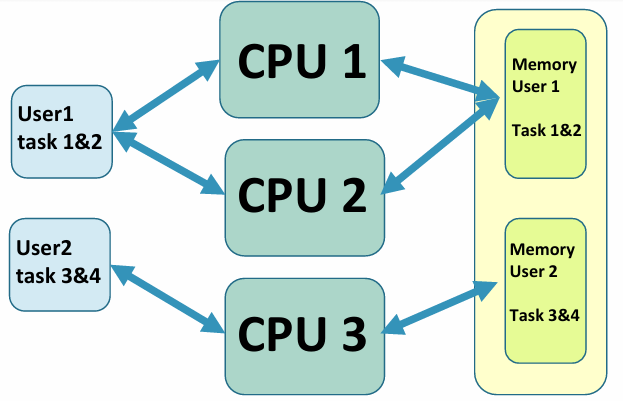
\includegraphics[width=0.4\textwidth]{figuresP/lesson_parallel_1_pag_29.png}
\end{center}

\subsubsection{- Multitasking}
We refer to \textbf{multitasking} when a single user has multiple tasks active at the same time. This is a general term from the user's perspective. It can be implemented via multiprogramming (on a single core) or true multiprocessing (on multiple cores). \\
In our example, one core plays Gangnam Style, and the other plays the heart-warming video. 

\begin{center}
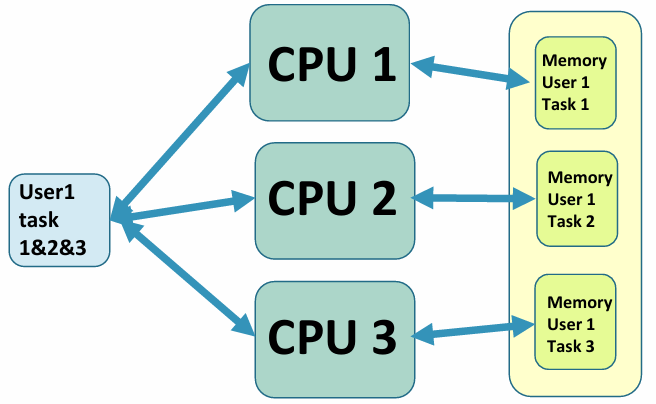
\includegraphics[width=0.4\textwidth]{figuresP/lesson_parallel_1_pag_30.png}
\end{center}

\subsubsection{- Distributed systems}
Lastly, in the so-called \textbf{distributed systems}, multiple computers even physically distant from one another can be used by the user to execute a single task. 

\begin{center}
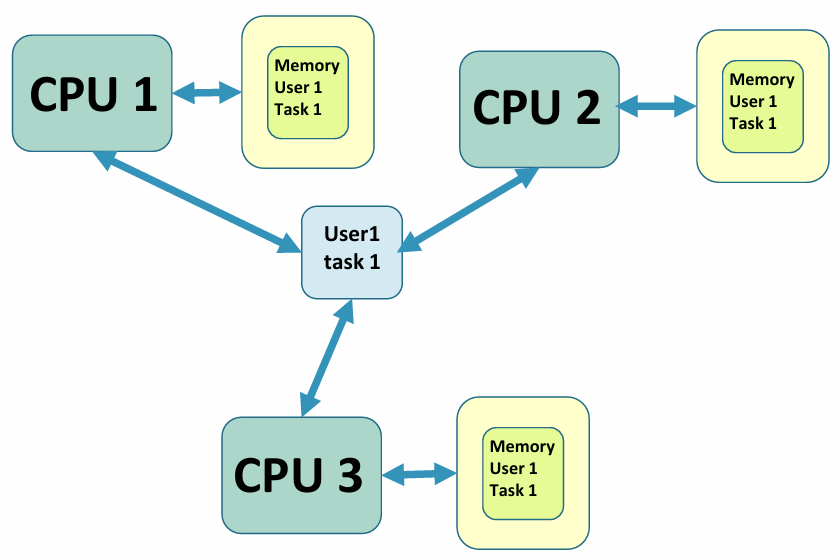
\includegraphics[width=0.4\textwidth]{figuresP/lesson_parallel_1_pag_31.png}
\end{center}

The advantages of concurrency are pretty obvious:
\begin{itemize}
    \item[-] Concurrent processes can reduce duplication;
    \item[-] The overall runtime of the algorithm can be significantly reduced;
    \item[-] More real-world problems can be solved than with sequential algorithms alone
\end{itemize}
However there are also many disadvantages:
\begin{itemize}
    \item[-] Runtime is not always reduced, so careful planning is required;
    \item[-] Concurrent algorithms can be more complex than sequential algorithms;
    \item[-] Shared data can be corrupted;
    \item[-] Communication between tasks is needed.
\end{itemize}

With that said, \textbf{what's the difference between concurrency and parallelization?} Concurrency is the execution of multiple tasks at the same time, regardless of the number of processors. Parallelism is the execution on multiple processors of the same task, which consists in breaking the task into meaningful pieces, doing the work on many processors, coordinating and putting the pieces back together.\\
More specifically, \textbf{concurrency is a property of the program structure}: it means dealing with multiple things at once (managing multiple start/end times). \textbf{Parallelism is a property of the machine execution}: it means doing multiple things at the exact same instant. A system can be concurrent without being parallel (e.g. multitasking on a single core via time-slicing) and can be parallel (e.g. bit-level instructions) without being concurrent. However, in high performance computing,\textit{ we typically aim for concurrency executed via parallelism to achieve maximum speed}. For example, imagine you have to render a 10-second video clip consisting of 300 frames.
\begin{itemize}
    \item[-] Concurrency (The Logic): The video editing software is designed to treat each frame as an independent task. The program creates 300 threads, one for each frame. This is concurrency: the structure allows multiple things to happen.
    \item[-] Parallelism (The Hardware): If you run this on a generic single-core laptop, the CPU will switch rapidly between frames (concurrency without parallelism). If you run this on a 16-core workstation, the CPU physically renders 16 frames at the exact same instant. This is concurrency executed via parallelism, resulting in a massive reduction of total execution time.
\end{itemize}

\subsection{Characteristics of task-level parallelization}
For a wide class of algorithms parallelization is the most powerful way to decrease execution time (not its complexity). For example, in a problem with $O(N\log N)$ complexity (e.g. quicksort) on $\log N$ processors should take the time needed by $O(N)$ algorithms. Or a problem with $O(N^2)$ complexity (e.g. bubble search) on N processors should take the time needed by $O(N)$ algorithms. As we will soon see, this is an oversimplified and (most of the time) wrong reasoning.

Parallelization is not free. Processors must be controlled and coordinated, i.e. we need a way to govern which processor does what work. The program must often be written in a special programming language for parallel systems and a parallelized program for one machine (with, say, 2K processors) might not be optimal on other machines (with, say, 2L processors).

Let's start by asking the most simple question: how much time can we gain from parallelizing an algorithm?
We define the \textbf{speed-up} as 
\begin{equation*}
    S_{n}=T_{s}  \ / \ T_{p}(n)    
\end{equation*}
where $T_{s}$ is the time needed to execute a task with a serial execution and $T_{p}(n)$ is the time needed to execute the same task with a parallel execution on $n$ processors. 
For a perfect parallel algorithm $S_{n}=n$. The vast majority of times, that is practically impossible, even if in very specific cases one could also have $S_{n}>n$ (\textit{superlinear case}).

With that in mind, we can also define the \textbf{efficiency} as 
\begin{equation*}
    E=S_{n}/n
\end{equation*}
It is a measure of how well our algorithm is using the processors. \\
Lastly, the \textbf{cost} is defined as
\begin{equation*}
    c=nT_{p}(n)=\frac{T_{1}}{E}
\end{equation*}
If we want to implement a certain algorithm using parallel processing, we also need to think about its \textbf{scalability}, which is the capability to remain efficient with an increasing number of processors.

Now that we have introduced some useful theoretical definitions, let's look at what happens in practice. What are the primary difficulties in implementing parallelization?
\begin{itemize}
    \item[-] \textbf{Load balancing}: In case of several tasks in parallel, the execution time of each task should be similar, otherwise the total time is dominated by the slower task. It's not easy to design a priori a parallel process with good load balancing, considering for instance that some of the available processors could be less efficient than others.
    \item[-] \textbf{Synchronization}: If the tasks use the same shared memory a logic of lock-unlock must be designed and the mechanism can involve a big latency
    \item[-] \textbf{Communication latency}: If data must be moved between processors, or most commonly between processors and memory, the overhead due to data transmission can be really relevant, to the point that it could make your parallel execution slower than a sequential one.
\end{itemize}
Moreover, \textit{Amdahl's law} (1967) shows one more big problem with parallelization. 

\subsection{Amdahl's law}
To easily understand the following concepts consider this example. You need to distribute 10000 flyers across the city and you have 11 workers at the office to help you. One of them has to go to the copy shop to get the 10000 flyers and the others need to distribute them. The first one does his job in an hour, the others take 1000 flyers each and in 6 hours they are done, for a total of 7 hours. How can you speed up this process? If you double the amount of workers that distribute flyers then the same job can be done in 4 hours (1+3). However, it doesn't make sense to send more than one person to get the flyers, since the time needed to reach the copy shop and come back would still be of 1 hour. That means that even with an infinite amount of workers, this job requires at least 1 hour to be completed.

This example shows us one fundamental idea: \textbf{not every part of a problem can be parallelized}. In fact, a problem that can be fully parallelized cannot exist. 

If only one part $(P_{K})$ of the problem can be improved, the maximum speed-up is given by:
\begin{equation*}
    S=1/\sum\frac{P_{K}}{S_{k}}    
\end{equation*}
where $k$ is the part of the problem and $S_{k}$ is the speed-up of $k$. That's \textbf{Amdahl's law}, which can be applied to every kind of problem. \\
In the case of parallel programming:
\begin{equation*}
    S_{n}=\frac{n}{na+(1-a)}    
\end{equation*}
where $a$ is the fraction of the code that cannot be parallelized.
If $n\rightarrow\infty$ the speed-up is $S_{n}=\frac{1}{a}$. Take a look at the image below. If the fraction of serial code is 10\% ($a=0.10$) the maximum speed-up is only 10 \textbf{regardless of the number of processors}. Even with tens of thousands of processors the results are scarce (for reference a 10x speed-up can be obtained just with a deep pipeline). 

\begin{center}
    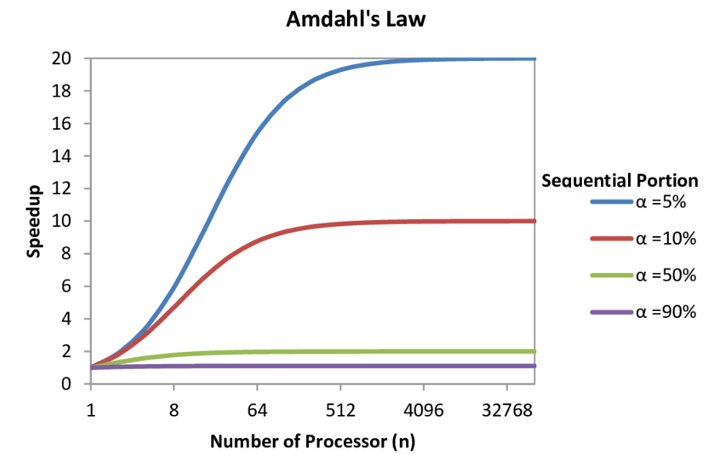
\includegraphics[width=0.6\textwidth]{figuresP/lesson_parallel_1_pag_36.png}
\end{center}

So apparently parallelism is useful only for "embarrassingly parallel" problems, with a small number of processors. Why bother, then?

Fortunately, there are important caveats to this law. One in particular is the key to solve all of our doubts on the usefulness of parallelism: Amdahl assumes that the dimension of the problem is always the same when increasing the number of processors, \textbf{but more processors means that wider problems can be addressed}. It's intuitive, but not trivial. 

In our example having 1000 workers is an obvious overkill if there are only 10000 flyers. However, with 1000 workers you could distribute a million flyers in 7 hours. The same thing goes with processors: 2 CPUs could easily compute the product of two $4\times4$ matrices, but for $1000\times1000$ matrices you are in need of much more processing power. 

In other words, Amdahl's law assumes that the \textit{scale} of the problem is fixed, which is absolutely not the case in the most useful applications of parallelism.

Lastly, Amdahl also assumes that the best solution is always the best serial algorithm but some problems require to be solved in parallel by their very nature. 

\subsection{Gustafson's law}
Let's define $t_s$ as the time of the serial part and $t_p$ as the time of the  parallel part. Now we take a problem that grows with the number of processors $n$ while the serial part remains always the same (e.g. when the number of flyers doubles, the number of workers does too). Under these assumptions, \textbf{Gustafson's law} (1988) tells us that the speed-up is given by:
\begin{equation*}
    S_{n}=n+(1-n)s 
\end{equation*}
That means that $S_n\propto n$, just like shown in the following figure.

\begin{center}
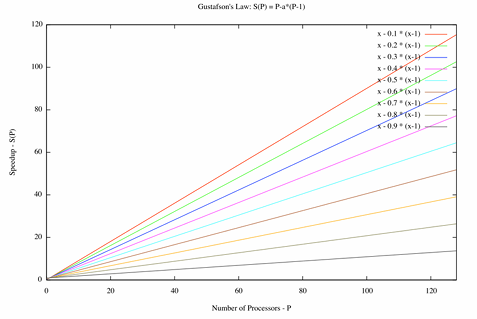
\includegraphics[width=0.5\textwidth]{figuresP/lesson_parallel_1_pag_39.png}
\end{center}

This last figure compares Amdahl's and Gustafson's law, showcasing how the speed-up changes when one assumes a fixed problem size or a fixed execution time respectively.

\begin{center}
    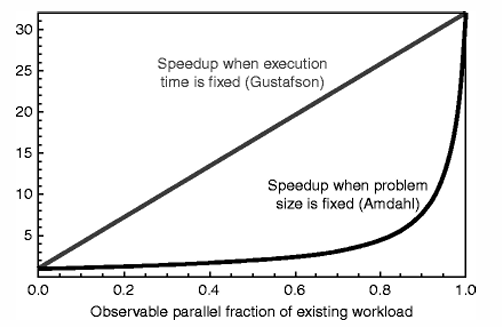
\includegraphics[width=0.5\textwidth]{figuresP/lesson_parallel_1_pag_39a.png}
\end{center}







\section{Multithreading and multiprocessing in Python}

\subsection{Introduction and some clarifications}

The fundamental question of this section is: \textbf{How do we actually implement parallelism in Python?} 

Before answering, here's an important consideration.

The term \textit{program} might sometimes be used in an improper way\footnote{By that I mean that I've surely used it improperly as a synonym of process and I will probably continue to do so in the next sections.}. Technically a program is a \textit{passive} entity, typically a file stored on disk, e.g. your \texttt{.py} files. It contains the instructions but does not consume CPU resources until executed. 

Also, do not mix up the definition of a thread and that of a process: a process is an independent instance of a program that is executed by the operating system. \textit{Each process runs in its own memory space and has its own resources}, which means it does not share memory directly with other processes. Instead, threads share the same memory space and you can think of them as (the smallest) parts of the same process! 

\begin{center}
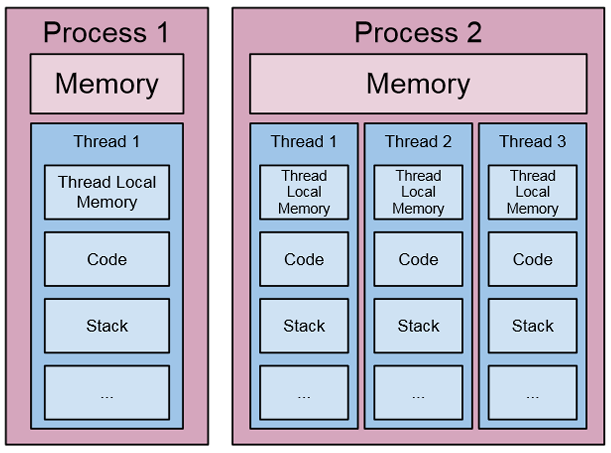
\includegraphics[width=0.5\textwidth]{figuresP/lesson_parallel_2A_pag_3.png}
\end{center}

Threads and processes are the fundamental blocks used to implement parallel programming in Python. 

A process could open another process during its execution (for example, if you run a Python program your code might launch an image editor) and the OS will have to assign resources and memory space to it accordingly. These processes don't "talk" to each other (unless you explicitly make them), which means for example that they don't share the same variables and functions. That makes them relatively less prone to some of the problems that we will soon talk about. They run independently and you can parallelize them with a multiprocessor. 

Threads are different. Parallelism happens when your code is written in a way that different operations can be completed simultaneously within the same memory space. That is riskier, but also much faster and lighter from the OS perspective, since it doesn't have to reassign anything. The term \textbf{Multithreading} refers to the simultaneous execution of different threads. 

\subsection{What not to do and how not to do it}
Parallel or concurrent execution (not only in Python) is very vulnerable to the following problems:
\begin{itemize}
    \item[-] \textbf{Starvation}: A task is constantly denied the necessary resources, so it can never finish ($\equiv$ it starves).
    \item[-] \textbf{Deadlock}: Two or more tasks wait cyclically for each other, causing a stall. 
    \begin{center}
        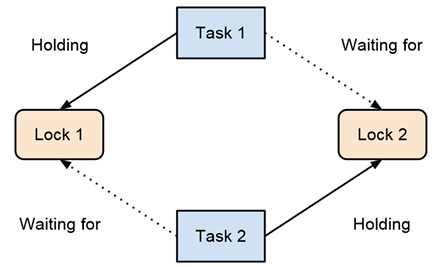
\includegraphics[width=0.35\textwidth]{figuresP/lesson_parallel_2A_pag_4.png}
    \end{center}
    \item[-] \textbf{Race condition}: A task that depends on the order of execution of the various threads or processes can produce wrongful results if such order is not respected. This is relevant for concurrency.
    \item[-] \textbf{Data corruption}: If two or more tasks try to work on the same memory location at the same time, the data you're working on can become corrupted during execution.
\end{itemize}
You need your program to be \textbf{thread-safe}, which means that it can be safely executed in a multithreaded environment without causing unexpected behaviour or errors, even when accessed by multiple threads simultaneously. Of course, that's going to take some careful programming, but fortunately there are some mechanisms that can help you avoid thread conflict.

For the most part, these are OS features that reserve the use of resources through synchronization primitives. For example, the \textbf{Mutex} is a locking mechanism: the first thread to require access to a certain memory location will be assigned a mutex token, it will access the memory and lock it so no other thread can interfere. Then the token passes onto the next thread and so on. The \textbf{Semaphore} system is a signalling mechanism that is just a generalization of the Mutex. A manager issues the ISR (Interrupt Signal Routing) and activates specific threads to avoid any conflict. \footnote{These mechanisms act on \textit{atomic operations}, at the lower level of the computer "brain".}

\subsection{The Global Interpreter Lock (GIL)}
Python implements a very simple thread-safe mechanism: the \textbf{Global Interpreter Lock (GIL)}. In order to prevent conflicts, only one statement in one thread is executed at a time (single-threading). In other words, the GIL seems to prevent multithreading, but don't worry: it can be deactivated. As of recent developments (e.g. Python 3.13+), there are ongoing efforts to make the GIL optional, but it remains a fundamental hurdle in standard environments.

Look at the following figure: there is a global lock that the current thread holds to safely access Python objects. Because only one thread can acquire Python Objects/C API, the interpreter regularly releases and reacquires the lock every 100 bytecodes of instructions. The frequency at which the interpreter checks for thread switching is controlled by the \texttt{sys.setcheckinterval()} function.

\begin{center}
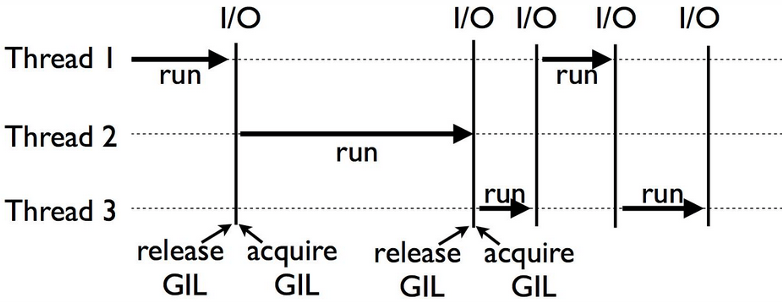
\includegraphics[width=0.6\textwidth]{figuresP/lesson_parallel_2A_pag_9.png}
\end{center}

There is only one exception to the global lock timing interval: the lock is released by a thread in case of an I/O operation, during which other threads can work concurrently. 

\begin{center}
    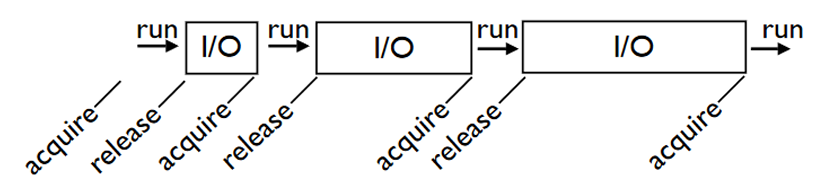
\includegraphics[width=0.6\textwidth]{figuresP/lesson_parallel_2A_pag_10.png}
\end{center}

It is important to note that, because of the GIL, CPU-bound applications won't be helped by threads. In Python, it is recommended to either use processes, or create a mixture of processes and threads. For this reason, \textit{Python is not the best language to use for parallelism}. So, what can we do? Python offers many libraries that provide wrappers for C functions. In other words, their classes and functions "steal" from the C language in order to let you work with parallelism.

Here's a short recap:

Pros and cons of processes:
\begin{itemize}
    \item[-] Can execute code simultaneously in the same Python program
    \item[-] Have separated memory space $\rightarrow$ less risky but difficult to communicate between them
    \item[-] Take advantage of multiple cores and CPUs
    \item[-] Avoid GIL limitations
    \item[-] Have relatively high overhead (opening and closing processes takes more time)
    \item[-] Child processes are killable
    \item[-] Model not adaptable to parallelism, better for concurrency
\end{itemize}

Pros and cons of threads:
\begin{itemize}
    \item[-] Use a shared memory $\rightarrow$ more risky (not in Python due to the GIL) but easier communication
    \item[-] Lightweight
    \item[-] Have very small overhead
    \item[-] Great option for I/O bound applications
    \item[-] Subject to GIL (although there are workarounds)
    \item[-] Not killable
    \item[-] Perfect for parallelism
\end{itemize}
So you should use\dots
\begin{itemize}
    \item[-] \dots\textit{processes} to speed up Python operations that are CPU intensive because they benefit from multiple cores and avoid the GIL.
    \item[-] \dots\textit{threads} for I/O tasks or tasks involving external systems because threads can combine their work more efficiently.
\end{itemize}

In the next sections we will (finally!) face some hands-on examples of parallel and concurrent computing in Python. You must learn how to use threads and processes, so we suggest you play along and write your own code. Also, during the in-person classes, these examples might have been analysed and explained a little more thoroughly than here, but if you've come this far you should have all the basics to understand what these new functions and classes do.

\subsection{Basics of multiprocessing in Python}

First of all, the basic modules needed to work with these mechanisms are \texttt{multiprocessing} and \texttt{threading}, so be sure you have them installed (they should already have been installed with your version of Python). The module \texttt{concurrent} (Python > 3.2) is an abstraction of multiprocessing and multithreading to simplify some functions.

Start by running \texttt{ps} on your Linux terminal. That will show all of your active processes:
\begin{verbatim}
lorenzo02@LAPTOP-AE9I3LPP:~/lezioni_computing_methods/parallel_python$ ps
    PID TTY          TIME CMD
    390 pts/0    00:00:00 bash
   9722 pts/0    00:00:00 ps
\end{verbatim}
With \texttt{ps -aux} you will be shown even the "hidden" processes (see documentation for more). 

\subsubsection{- First simple example: \texttt{Process}, \texttt{.start()}, \texttt{.join()}}
Take a look at the code below. The \texttt{Process} class from the \texttt{multiprocessing} module lets you easily manage processes in your code. The \texttt{.start()} method starts the execution of the child process (this is when the OS allocates memory space and resources for \texttt{p}). The \texttt{.join()} method tells the main process to wait for \texttt{p} to finish before continuing with its execution.

\begin{Verbatim}[label=\makebox{\url{https://github.com/lucabaldini/cmepda/tree/master/slides/latex/snippets/hello_multiprocessing.py}},commandchars=\\\{\}]
\PY{k}{from} \PY{n+nn}{multiprocessing} \PY{k}{import} \PY{n}{Process}

\PY{c+c1}{\# Defining a simple function...}
\PY{k}{def} \PY{n+nf}{f}\PY{p}{(}\PY{n}{name}\PY{p}{)}\PY{p}{:}
    \PY{n+nb}{print}\PY{p}{(}\PY{l+s+s1}{\PYZsq{}}\PY{l+s+s1}{Hello }\PY{l+s+s1}{\PYZsq{}}\PY{o}{+}\PY{n}{name}\PY{p}{)}

\PY{c+c1}{\# The function is execued in a child process,}
\PY{c+c1}{\# different than the one that was created by the HelloWorld.py program.}
\PY{k}{if} \PY{n}{\_\_name\_\_}\PY{o}{==}\PY{l+s+s2}{\PYZdq{}}\PY{l+s+s2}{\_\_main\_\_}\PY{l+s+s2}{\PYZdq{}}\PY{p}{:}
    \PY{n}{p} \PY{o}{=} \PY{n}{Process}\PY{p}{(}\PY{n}{target}\PY{o}{=}\PY{n}{f}\PY{p}{,} \PY{n}{args}\PY{o}{=}\PY{p}{(}\PY{l+s+s1}{\PYZsq{}}\PY{l+s+s1}{World}\PY{l+s+s1}{\PYZsq{}}\PY{p}{,}\PY{p}{)}\PY{p}{)}
    \PY{n}{p}\PY{o}{.}\PY{n}{start}\PY{p}{(}\PY{p}{)}
    \PY{n}{p}\PY{o}{.}\PY{n}{join}\PY{p}{(}\PY{p}{)}

[Output]
Hello World
\end{Verbatim}

\subsubsection{- Father and Sons}

If you run \texttt{ps} in your terminal, you will find that each process has a unique number called PID. In Python \texttt{os.getpid()} returns the PID of the current process, while \texttt{os.getppid()} executed in a secondary process (the child) returns the PID of the main one (the father). Pay attention to the PID numbers in the following example, which generates a tree of processes just like the one in the figure (PID numbers may vary):

\begin{Verbatim}[label=\makebox{\url{https://github.com/lucabaldini/cmepda/tree/master/slides/latex/snippets/FatherAndSons.py}},commandchars=\\\{\}]
\PY{k}{from} \PY{n+nn}{multiprocessing} \PY{k}{import} \PY{n}{Process}
\PY{k}{import} \PY{n+nn}{os}
\PY{k}{def} \PY{n+nf}{f0}\PY{p}{(}\PY{n}{name}\PY{p}{)}\PY{p}{:}
    \PY{n+nb}{print}\PY{p}{(}\PY{p}{)}
    \PY{n+nb}{print}\PY{p}{(}\PY{l+s+s2}{\PYZdq{}}\PY{l+s+s2}{\PYZhy{}\PYZhy{}\PYZhy{}\PYZhy{}\PYZgt{} function }\PY{l+s+s2}{\PYZdq{}}\PY{o}{+}\PY{n}{name}\PY{p}{)}
    \PY{n+nb}{print} \PY{p}{(}\PY{l+s+s2}{\PYZdq{}}\PY{l+s+s2}{I am still the main process with ID }\PY{l+s+s2}{\PYZdq{}}
           \PY{o}{+}\PY{n+nb}{str}\PY{p}{(}\PY{n}{os}\PY{o}{.}\PY{n}{getpid}\PY{p}{(}\PY{p}{)}\PY{p}{)}\PY{o}{+}\PY{l+s+s2}{\PYZdq{}}\PY{l+s+s2}{ my father is ID:}\PY{l+s+s2}{\PYZdq{}}\PY{o}{+}\PY{n+nb}{str}\PY{p}{(}\PY{n}{os}\PY{o}{.}\PY{n}{getppid}\PY{p}{(}\PY{p}{)}\PY{p}{)}\PY{p}{)}

\PY{k}{def} \PY{n+nf}{f1}\PY{p}{(}\PY{n}{name}\PY{p}{)}\PY{p}{:}
    \PY{n+nb}{print}\PY{p}{(}\PY{p}{)}
    \PY{n+nb}{print}\PY{p}{(}\PY{l+s+s2}{\PYZdq{}}\PY{l+s+s2}{\PYZhy{}\PYZhy{}\PYZhy{}\PYZhy{}\PYZgt{} function }\PY{l+s+s2}{\PYZdq{}}\PY{o}{+}\PY{n}{name}\PY{p}{)}
    \PY{n+nb}{print} \PY{p}{(}\PY{l+s+s2}{\PYZdq{}}\PY{l+s+s2}{I am the first sub\PYZhy{}process with ID }\PY{l+s+s2}{\PYZdq{}}
           \PY{o}{+}\PY{n+nb}{str}\PY{p}{(}\PY{n}{os}\PY{o}{.}\PY{n}{getpid}\PY{p}{(}\PY{p}{)}\PY{p}{)}\PY{o}{+}\PY{l+s+s2}{\PYZdq{}}\PY{l+s+s2}{ my father is ID:}\PY{l+s+s2}{\PYZdq{}}\PY{o}{+}\PY{n+nb}{str}\PY{p}{(}\PY{n}{os}\PY{o}{.}\PY{n}{getppid}\PY{p}{(}\PY{p}{)}\PY{p}{)}\PY{p}{)}
    \PY{n}{f2}\PY{p}{(}\PY{l+s+s1}{\PYZsq{}}\PY{l+s+s1}{two}\PY{l+s+s1}{\PYZsq{}}\PY{p}{)}


\PY{k}{def} \PY{n+nf}{f2}\PY{p}{(}\PY{n}{name}\PY{p}{)}\PY{p}{:}
    \PY{n+nb}{print}\PY{p}{(}\PY{p}{)}
    \PY{n+nb}{print}\PY{p}{(}\PY{l+s+s2}{\PYZdq{}}\PY{l+s+s2}{\PYZhy{}\PYZhy{}\PYZhy{}\PYZhy{}\PYZgt{} function }\PY{l+s+s2}{\PYZdq{}}\PY{o}{+}\PY{n}{name}\PY{p}{)}
    \PY{n+nb}{print} \PY{p}{(}\PY{l+s+s2}{\PYZdq{}}\PY{l+s+s2}{I am still the first sub\PYZhy{}process with ID }\PY{l+s+s2}{\PYZdq{}}
           \PY{o}{+}\PY{n+nb}{str}\PY{p}{(}\PY{n}{os}\PY{o}{.}\PY{n}{getpid}\PY{p}{(}\PY{p}{)}\PY{p}{)}\PY{o}{+}\PY{l+s+s2}{\PYZdq{}}\PY{l+s+s2}{ my father is ID:}\PY{l+s+s2}{\PYZdq{}}\PY{o}{+}\PY{n+nb}{str}\PY{p}{(}\PY{n}{os}\PY{o}{.}\PY{n}{getppid}\PY{p}{(}\PY{p}{)}\PY{p}{)}\PY{p}{)}
    \PY{n+nb}{print}\PY{p}{(}\PY{l+s+s2}{\PYZdq{}}\PY{l+s+s2}{This is the end!}\PY{l+s+s2}{\PYZdq{}}\PY{p}{)}

\PY{c+c1}{\#MAIN}
\PY{k}{if} \PY{n}{\_\_name\_\_}\PY{o}{==}\PY{l+s+s2}{\PYZdq{}}\PY{l+s+s2}{\_\_main\_\_}\PY{l+s+s2}{\PYZdq{}}\PY{p}{:}
    \PY{n+nb}{print} \PY{p}{(}\PY{l+s+s2}{\PYZdq{}}\PY{l+s+s2}{I am the main process with ID: }\PY{l+s+s2}{\PYZdq{}}\PY{o}{+}\PY{n+nb}{str}\PY{p}{(}\PY{n}{os}\PY{o}{.}\PY{n}{getpid}\PY{p}{(}\PY{p}{)}\PY{p}{)}\PY{p}{)}
    \PY{n}{f0}\PY{p}{(}\PY{l+s+s1}{\PYZsq{}}\PY{l+s+s1}{zero}\PY{l+s+s1}{\PYZsq{}}\PY{p}{)}
    \PY{n}{p} \PY{o}{=} \PY{n}{Process}\PY{p}{(}\PY{n}{target}\PY{o}{=}\PY{n}{f1}\PY{p}{,} \PY{n}{args}\PY{o}{=}\PY{p}{(}\PY{l+s+s1}{\PYZsq{}}\PY{l+s+s1}{one}\PY{l+s+s1}{\PYZsq{}}\PY{p}{,}\PY{p}{)}\PY{p}{)}
    \PY{n}{p}\PY{o}{.}\PY{n}{start}\PY{p}{(}\PY{p}{)}
    \PY{n}{p}\PY{o}{.}\PY{n}{join}\PY{p}{(}\PY{p}{)}

[Output]
I am the main process with ID:2420

-----> function zero
I am still the main process with ID 3384 my father is ID:2420

-----> function one
I am the first sub-process with ID 3385 my father is ID:3384

-----> function two
I am still the first sub-process with ID 3385 my father is ID:3384
This is the end!
\end{Verbatim}

\begin{center}
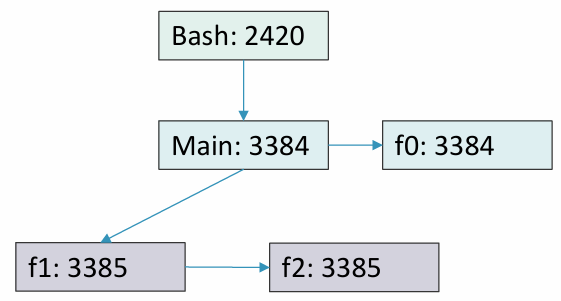
\includegraphics[width=0.4\textwidth]{figuresP/lesson_parallel_2B_pag_8}
\end{center}

Note: You might not be familiar with the \texttt{if \_\_name\_\_ == "\_\_main\_\_"} line, but it's very common in Python programming. It's there only so that if you import that module you won't automatically run the code under the \texttt{if} statement. The name of your process is \texttt{"\_\_main\_\_"} only if you run that program directly. 

\subsubsection{- Function on 4 processes: the \texttt{Queue}}

What if you wanted to run the same function on 4 different processes? You need to use a \texttt{Queue}.

The \texttt{Queue} class lets you create and manage a queue of processes, and it's the "letterbox" that lets such processes send variables to the main one: \texttt{Queue.put()} inserts an object in the queue while \texttt{Queue.get()} extracts an object from it. Here's how to use them:

\begin{Verbatim}[label=\makebox{\url{https://github.com/lucabaldini/cmepda/tree/master/slides/latex/snippets/multiprocessing_queue.py}},commandchars=\\\{\}]
\PY{k}{import} \PY{n+nn}{multiprocessing} \PY{k}{as} \PY{n+nn}{mp}

\PY{c+c1}{\# Define an example function}
\PY{k}{def} \PY{n+nf}{Hello}\PY{p}{(}\PY{n}{pos}\PY{p}{,}\PY{n}{name}\PY{p}{)}\PY{p}{:}
    \PY{n}{msg}\PY{o}{=}\PY{l+s+s2}{\PYZdq{}}\PY{l+s+s2}{Hello }\PY{l+s+s2}{\PYZdq{}}\PY{o}{+}\PY{n}{name}
    \PY{n}{output}\PY{o}{.}\PY{n}{put}\PY{p}{(}\PY{p}{(}\PY{n}{pos}\PY{p}{,} \PY{n}{msg}\PY{p}{)}\PY{p}{)}

\PY{k}{if} \PY{n}{\_\_name\_\_}\PY{o}{==}\PY{l+s+s2}{\PYZdq{}}\PY{l+s+s2}{\_\_main\_\_}\PY{l+s+s2}{\PYZdq{}}\PY{p}{:}
    \PY{c+c1}{\# Define an output queue}
    \PY{n}{output} \PY{o}{=} \PY{n}{mp}\PY{o}{.}\PY{n}{Queue}\PY{p}{(}\PY{p}{)}
    \PY{c+c1}{\# Setup a list of processes that we want to run}
    \PY{n}{processes} \PY{o}{=} \PY{p}{[}\PY{n}{mp}\PY{o}{.}\PY{n}{Process}\PY{p}{(}\PY{n}{target}\PY{o}{=}\PY{n}{Hello}\PY{p}{,} \PY{n}{args}\PY{o}{=}\PY{p}{(}\PY{n}{x}\PY{p}{,} \PY{l+s+s2}{\PYZdq{}}\PY{l+s+s2}{Gianluca}\PY{l+s+s2}{\PYZdq{}}\PY{p}{)}\PY{p}{)} \PY{k}{for} \PY{n}{x} \PY{k}{in} \PY{n+nb}{range}\PY{p}{(}\PY{l+m+mi}{4}\PY{p}{)}\PY{p}{]}
    
    \PY{c+c1}{\# Run processes}
    \PY{k}{for} \PY{n}{p} \PY{k}{in} \PY{n}{processes}\PY{p}{:}
        \PY{n}{p}\PY{o}{.}\PY{n}{start}\PY{p}{(}\PY{p}{)}

    \PY{c+c1}{\# Exit the completed processes}
    \PY{k}{for} \PY{n}{p} \PY{k}{in} \PY{n}{processes}\PY{p}{:}
        \PY{n}{p}\PY{o}{.}\PY{n}{join}\PY{p}{(}\PY{p}{)}
            
    \PY{c+c1}{\# Get process results from the output queue}
    \PY{n}{results} \PY{o}{=} \PY{p}{[}\PY{n}{output}\PY{o}{.}\PY{n}{get}\PY{p}{(}\PY{p}{)} \PY{k}{for} \PY{n}{p} \PY{k}{in} \PY{n}{processes}\PY{p}{]}
    \PY{n+nb}{print}\PY{p}{(}\PY{n}{results}\PY{p}{)}

[Output]
[(0, 'Hello Gianluca'), (1, 'Hello Gianluca'), (2, 'Hello Gianluca'), (3, 'Hello Gianluca')]
\end{Verbatim}

\subsubsection{- Distributing your work: the \texttt{Pool}}

Using the \texttt{Pool} class, you can define a certain number of processes that will run on different cores (if your computer has more than one). Take a look at the code below:
\begin{itemize}
    \item[-] \texttt{Pool.map()} stops the execution of the main program and runs your processes (\textit{synchronous run});
    \item[-] \texttt{Pool.map\_async()} runs your processes without stopping the main one. That's why in the second example you need a \texttt{timeout} before retrieving the results: you have to make sure that your processes are done (\textit{asynchronous run}). 
\end{itemize}
Pay attention to the PID numbers: can you tell in what order and by which process the 6 operations were executed? 

See also the documentation for  \texttt{Pool.apply()} and \texttt{Pool.apply\_async()}, which have similar effects. 

Here is an example demonstrating the synchronous \texttt{Pool.map()}:

\begin{Verbatim}[label=\makebox{\url{https://github.com/lucabaldini/cmepda/tree/master/slides/latex/snippets/multiprocessing_pool_map.py}},commandchars=\\\{\}]
\PY{k}{import} \PY{n+nn}{multiprocessing} \PY{k}{as} \PY{n+nn}{mp}
\PY{k}{import} \PY{n+nn}{time}
\PY{k}{import} \PY{n+nn}{os}

\PY{k}{def} \PY{n+nf}{cube}\PY{p}{(}\PY{n}{x}\PY{p}{)}\PY{p}{:}
    \PY{n+nb}{print} \PY{p}{(}\PY{n+nb}{str}\PY{p}{(}\PY{n}{os}\PY{o}{.}\PY{n}{getpid}\PY{p}{(}\PY{p}{)}\PY{p}{)}\PY{o}{+}\PY{l+s+s2}{\PYZdq{}}\PY{l+s+s2}{ }\PY{l+s+s2}{\PYZdq{}}\PY{o}{+}\PY{n+nb}{str}\PY{p}{(}\PY{n}{os}\PY{o}{.}\PY{n}{getppid}\PY{p}{(}\PY{p}{)}\PY{p}{)}\PY{o}{+}\PY{l+s+s2}{\PYZdq{}}\PY{l+s+s2}{ }\PY{l+s+s2}{\PYZdq{}}\PY{o}{+}\PY{n+nb}{str}\PY{p}{(}\PY{n}{x}\PY{o}{**}\PY{l+m+mi}{3}\PY{p}{)}\PY{p}{)}
    \PY{k}{return} \PY{n}{x}\PY{o}{**}\PY{l+m+mi}{3}

\PY{k}{if} \PY{n}{\_\_name\_\_}\PY{o}{==}\PY{l+s+s2}{\PYZdq{}}\PY{l+s+s2}{\_\_main\_\_}\PY{l+s+s2}{\PYZdq{}}\PY{p}{:}
    \PY{c+c1}{\# Define a group of processes (\PYZdq{}workers\PYZdq{})}
    \PY{n}{pool} \PY{o}{=} \PY{n}{mp}\PY{o}{.}\PY{n}{Pool}\PY{p}{(}\PY{n}{processes}\PY{o}{=}\PY{l+m+mi}{4}\PY{p}{)}
    \PY{c+c1}{\# Make each worker do something (even if \# tasks \PYZgt{} \# workers)}
    \PY{n}{results} \PY{o}{=} \PY{n}{pool}\PY{o}{.}\PY{n}{map}\PY{p}{(}\PY{n}{cube}\PY{p}{,} \PY{n+nb}{range}\PY{p}{(}\PY{l+m+mi}{1}\PY{p}{,}\PY{l+m+mi}{7}\PY{p}{)}\PY{p}{)}
    \PY{c+c1}{\# Print the results}
    \PY{n+nb}{print}\PY{p}{(}\PY{n}{results}\PY{p}{)}

[Output]
17348 17346 8
17347 17346 1
17349 17346 27
17350 17346 64
17348 17346 125
17347 17346 216
[1, 8, 27, 64, 125, 216]
\end{Verbatim}
\bigskip
\hrulefill
\bigskip

And here is the asynchronous equivalent using \texttt{Pool.map\_async()}:

\begin{Verbatim}[label=\makebox{\url{https://github.com/lucabaldini/cmepda/tree/master/slides/latex/snippets/multiprocessing_map_async_timeout.py}},commandchars=\\\{\}]
\PY{k}{import} \PY{n+nn}{multiprocessing} \PY{k}{as} \PY{n+nn}{mp}
\PY{k}{import} \PY{n+nn}{os}

\PY{k}{def} \PY{n+nf}{cube}\PY{p}{(}\PY{n}{x}\PY{p}{)}\PY{p}{:}
    \PY{n+nb}{print} \PY{p}{(}\PY{n+nb}{str}\PY{p}{(}\PY{n}{os}\PY{o}{.}\PY{n}{getpid}\PY{p}{(}\PY{p}{)}\PY{p}{)}\PY{o}{+}\PY{l+s+s2}{\PYZdq{}}\PY{l+s+s2}{ }\PY{l+s+s2}{\PYZdq{}}\PY{o}{+}\PY{n+nb}{str}\PY{p}{(}\PY{n}{os}\PY{o}{.}\PY{n}{getppid}\PY{p}{(}\PY{p}{)}\PY{p}{)}\PY{o}{+}\PY{l+s+s2}{\PYZdq{}}\PY{l+s+s2}{ }\PY{l+s+s2}{\PYZdq{}}\PY{o}{+}\PY{n+nb}{str}\PY{p}{(}\PY{n}{x}\PY{o}{**}\PY{l+m+mi}{3}\PY{p}{)}\PY{p}{)}
    \PY{k}{return} \PY{n}{x}\PY{o}{**}\PY{l+m+mi}{3}

\PY{k}{if} \PY{n}{\_\_name\_\_}\PY{o}{==}\PY{l+s+s2}{\PYZdq{}}\PY{l+s+s2}{\_\_main\_\_}\PY{l+s+s2}{\PYZdq{}}\PY{p}{:}
    \PY{c+c1}{\# Define a group of processes (\PYZdq{}workers\PYZdq{})}
    \PY{n}{pool} \PY{o}{=} \PY{n}{mp}\PY{o}{.}\PY{n}{Pool}\PY{p}{(}\PY{n}{processes}\PY{o}{=}\PY{l+m+mi}{4}\PY{p}{)}
    \PY{c+c1}{\# Make each worker do something without interrupting the main process}
    \PY{n}{results} \PY{o}{=} \PY{n}{pool}\PY{o}{.}\PY{n}{map\_async}\PY{p}{(}\PY{n}{cube}\PY{p}{,} \PY{n+nb}{range}\PY{p}{(}\PY{l+m+mi}{1}\PY{p}{,}\PY{l+m+mi}{7}\PY{p}{)}\PY{p}{)}
    \PY{c+c1}{\# Print the results using a timeout to be sure results is full}
    \PY{n+nb}{print}\PY{p}{(}\PY{n}{results}\PY{o}{.}\PY{n}{get}\PY{p}{(}\PY{n}{timeout}\PY{o}{=}\PY{l+m+mi}{1}\PY{p}{)}\PY{p}{)}

[Output]
17428 17425 1
17429 17425 8
17428 17425 64
17428 17425 216
17431 17425 125
17430 17425 27
[1, 8, 27, 64, 125, 216]
\end{Verbatim}

Let's create a function with a "sleep" time using the \texttt{time} module to simulate a longer execution. Take a look at the two versions of the code. In the synchronous example, the time needed to execute the main process is about 6 seconds (since it has to wait for the child processes, 3 + 3 seconds) while in the asynchronous one the \texttt{elapsed\_time} is less than a second. Of course, the latter didn't actually run faster, but we closed the main process before the others had ended (in fact, the output seems truncated). In this case our function doesn't return anything, otherwise our \texttt{timeout} would have slowed the main process down. 

\begin{Verbatim}[label=\makebox{\url{https://github.com/lucabaldini/cmepda/tree/master/slides/latex/snippets/multiprocessing_pool_doingstuff.py}},commandchars=\\\{\}]
\PY{k}{import} \PY{n+nn}{multiprocessing} \PY{k}{as} \PY{n+nn}{mp}
\PY{k}{import} \PY{n+nn}{time}
\PY{k}{import} \PY{n+nn}{os}

\PY{k}{def} \PY{n+nf}{doingstuff}\PY{p}{(}\PY{n}{x}\PY{p}{)}\PY{p}{:}
    \PY{n+nb}{print} \PY{p}{(}\PY{l+s+s2}{\PYZdq{}}\PY{l+s+s2}{Process: }\PY{l+s+s2}{\PYZdq{}}\PY{o}{+}\PY{n+nb}{str}\PY{p}{(}\PY{n}{x}\PY{p}{)}\PY{o}{+}\PY{l+s+s2}{\PYZdq{}}\PY{l+s+s2}{ }\PY{l+s+s2}{\PYZdq{}}\PY{o}{+}\PY{n+nb}{str}\PY{p}{(}\PY{n}{os}\PY{o}{.}\PY{n}{getpid}\PY{p}{(}\PY{p}{)}\PY{p}{)}\PY{p}{)}
    \PY{c+c1}{\# Add a delay}
    \PY{n}{time}\PY{o}{.}\PY{n}{sleep}\PY{p}{(}\PY{l+m+mi}{3}\PY{p}{)}

\PY{k}{if} \PY{n}{\_\_name\_\_}\PY{o}{==}\PY{l+s+s2}{\PYZdq{}}\PY{l+s+s2}{\_\_main\_\_}\PY{l+s+s2}{\PYZdq{}}\PY{p}{:}
    \PY{c+c1}{\# Start the timer}
    \PY{n}{start}\PY{o}{=}\PY{n}{time}\PY{o}{.}\PY{n}{time}\PY{p}{(}\PY{p}{)}
    \PY{c+c1}{\# Define a group of processes (\PYZdq{}workers\PYZdq{})}
    \PY{n}{pool} \PY{o}{=} \PY{n}{mp}\PY{o}{.}\PY{n}{Pool}\PY{p}{(}\PY{n}{processes}\PY{o}{=}\PY{l+m+mi}{4}\PY{p}{)}
    \PY{c+c1}{\# Make each worker do something}
    \PY{n}{results} \PY{o}{=} \PY{n}{pool}\PY{o}{.}\PY{n}{map}\PY{p}{(}\PY{n}{doingstuff}\PY{p}{,} \PY{n+nb}{range}\PY{p}{(}\PY{l+m+mi}{1}\PY{p}{,}\PY{l+m+mi}{10}\PY{p}{)}\PY{p}{)}
    \PY{c+c1}{\# Stop the timer}
    \PY{n}{end}\PY{o}{=}\PY{n}{time}\PY{o}{.}\PY{n}{time}\PY{p}{(}\PY{p}{)}
    \PY{n+nb}{print}\PY{p}{(}\PY{l+s+s2}{\PYZdq{}}\PY{l+s+s2}{elapsed time: }\PY{l+s+s2}{\PYZdq{}}\PY{o}{+}\PY{n+nb}{str}\PY{p}{(}\PY{n}{end}\PY{o}{\PYZhy{}}\PY{n}{start}\PY{p}{)}\PY{p}{)}

[Output]
Process: 1 19112
Process: 2 19113
Process: 3 19114
Process: 4 19115
Process: 5 19112
Process: 6 19113
Process: 7 19114
Process: 8 19115
Process: 9 19113
elapsed time: 9.066443681716919
\end{Verbatim}
\bigskip
\hrulefill
\bigskip

\begin{Verbatim}[label=\makebox{\url{https://github.com/lucabaldini/cmepda/tree/master/slides/latex/snippets/multiprocessing_pool_doingstuff_async.py}},commandchars=\\\{\}]
\PY{k}{import} \PY{n+nn}{multiprocessing} \PY{k}{as} \PY{n+nn}{mp}
\PY{k}{import} \PY{n+nn}{time}
\PY{k}{import} \PY{n+nn}{os}

\PY{k}{def} \PY{n+nf}{doingstuff}\PY{p}{(}\PY{n}{x}\PY{p}{)}\PY{p}{:}
    \PY{n+nb}{print} \PY{p}{(}\PY{l+s+s2}{\PYZdq{}}\PY{l+s+s2}{Process: }\PY{l+s+s2}{\PYZdq{}}\PY{o}{+}\PY{n+nb}{str}\PY{p}{(}\PY{n}{x}\PY{p}{)}\PY{o}{+}\PY{l+s+s2}{\PYZdq{}}\PY{l+s+s2}{ }\PY{l+s+s2}{\PYZdq{}}\PY{o}{+}\PY{n+nb}{str}\PY{p}{(}\PY{n}{os}\PY{o}{.}\PY{n}{getpid}\PY{p}{(}\PY{p}{)}\PY{p}{)}\PY{p}{)}
    \PY{c+c1}{\# Add a delay}
    \PY{n}{time}\PY{o}{.}\PY{n}{sleep}\PY{p}{(}\PY{l+m+mi}{3}\PY{p}{)}

\PY{k}{if} \PY{n}{\_\_name\_\_}\PY{o}{==}\PY{l+s+s2}{\PYZdq{}}\PY{l+s+s2}{\_\_main\_\_}\PY{l+s+s2}{\PYZdq{}}\PY{p}{:}
    \PY{c+c1}{\# Start the timer}
    \PY{n}{start}\PY{o}{=}\PY{n}{time}\PY{o}{.}\PY{n}{time}\PY{p}{(}\PY{p}{)}
    \PY{c+c1}{\# Define a group of processes (\PYZdq{}workers\PYZdq{})}
    \PY{n}{pool} \PY{o}{=} \PY{n}{mp}\PY{o}{.}\PY{n}{Pool}\PY{p}{(}\PY{n}{processes}\PY{o}{=}\PY{l+m+mi}{4}\PY{p}{)}
    \PY{c+c1}{\# Make each worker do something}
    \PY{n}{results} \PY{o}{=} \PY{n}{pool}\PY{o}{.}\PY{n}{map\_async}\PY{p}{(}\PY{n}{doingstuff}\PY{p}{,} \PY{n+nb}{range}\PY{p}{(}\PY{l+m+mi}{1}\PY{p}{,}\PY{l+m+mi}{10}\PY{p}{)}\PY{p}{)}
    \PY{c+c1}{\# Stop the timer}
    \PY{n}{end}\PY{o}{=}\PY{n}{time}\PY{o}{.}\PY{n}{time}\PY{p}{(}\PY{p}{)}
    \PY{n+nb}{print}\PY{p}{(}\PY{l+s+s2}{\PYZdq{}}\PY{l+s+s2}{elapsed time: }\PY{l+s+s2}{\PYZdq{}}\PY{o}{+}\PY{n+nb}{str}\PY{p}{(}\PY{n}{end}\PY{o}{\PYZhy{}}\PY{n}{start}\PY{p}{)}\PY{p}{)}

[Output]
elapsed time: 0.028638362884521484
Process: 1 19211
Process: 2 19212
Process: 3 19213
Process: 4 19214
\end{Verbatim}

\subsection{Communicating processes in Python}

\subsubsection{- Shared memory}

In the following code a dangerous mechanism is shown: the main process and the child one seem to share a global variable, but the result is a disaster!

\begin{Verbatim}[label=\makebox{\url{https://github.com/lucabaldini/cmepda/tree/master/slides/latex/snippets/multiprocessing_global_scope.py}},commandchars=\\\{\}]
\PY{k}{import} \PY{n+nn}{multiprocessing}

\PY{c+c1}{\# Empty list with global scope}
\PY{n}{result} \PY{o}{=} \PY{p}{[}\PY{p}{]}

\PY{k}{def} \PY{n+nf}{square\_list}\PY{p}{(}\PY{n}{mylist}\PY{p}{)}\PY{p}{:}
        \PY{k}{global} \PY{n}{result}
        \PY{k}{for} \PY{n}{num} \PY{k}{in} \PY{n}{mylist}\PY{p}{:}
                \PY{n}{result}\PY{o}{.}\PY{n}{append}\PY{p}{(}\PY{n}{num} \PY{o}{*} \PY{n}{num}\PY{p}{)}
        \PY{c+c1}{\# Print result list from the function}
        \PY{n+nb}{print}\PY{p}{(}\PY{l+s+s2}{\PYZdq{}}\PY{l+s+s2}{Result(in process p1): }\PY{l+s+s2}{\PYZdq{}}\PY{o}{+}\PY{n+nb}{str}\PY{p}{(}\PY{n}{result}\PY{p}{)}\PY{p}{)}

\PY{k}{if} \PY{n}{\_\_name\_\_}\PY{o}{==}\PY{l+s+s2}{\PYZdq{}}\PY{l+s+s2}{\_\_main\_\_}\PY{l+s+s2}{\PYZdq{}}\PY{p}{:}
    \PY{c+c1}{\# Input list}
    \PY{n}{mylist} \PY{o}{=} \PY{p}{[}\PY{l+m+mi}{1}\PY{p}{,}\PY{l+m+mi}{2}\PY{p}{,}\PY{l+m+mi}{3}\PY{p}{,}\PY{l+m+mi}{4}\PY{p}{]}
    \PY{c+c1}{\# Creating the new process}
    \PY{n}{p1} \PY{o}{=} \PY{n}{multiprocessing}\PY{o}{.}\PY{n}{Process}\PY{p}{(}\PY{n}{target}\PY{o}{=}\PY{n}{square\_list}\PY{p}{,} \PY{n}{args}\PY{o}{=}\PY{p}{(}\PY{n}{mylist}\PY{p}{,}\PY{p}{)}\PY{p}{)}
    \PY{n}{p1}\PY{o}{.}\PY{n}{start}\PY{p}{(}\PY{p}{)}
    \PY{n}{p1}\PY{o}{.}\PY{n}{join}\PY{p}{(}\PY{p}{)}
    \PY{c+c1}{\# Print global result list}
    \PY{n+nb}{print}\PY{p}{(}\PY{l+s+s2}{\PYZdq{}}\PY{l+s+s2}{Result(in main program): }\PY{l+s+s2}{\PYZdq{}}\PY{o}{+}\PY{n+nb}{str}\PY{p}{(}\PY{n}{result}\PY{p}{)}\PY{p}{)}

[Output]
Result(in process p1): [1, 4, 9, 16]
Result(in main program): []
\end{Verbatim}

Always remember: different processes have different memory spaces, so the \texttt{result} variable is not modified in the main process. 

In order to correctly work out this task, you can create a shared memory space between the two processes. Here this is done using the \texttt{Array} and the \texttt{Value} classes, which respectively create a "location" (we will see that the correct term is \textit{pointer}) in the shared memory for an array and for a value. In this example, we fill these locations with the results of our processes. 

\begin{center}
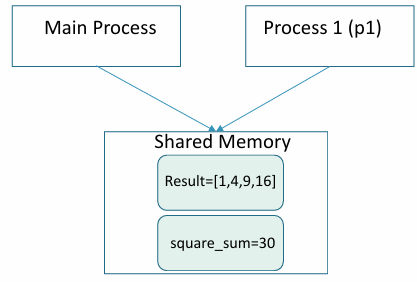
\includegraphics[width=0.4\textwidth]{figuresP/lesson_parallel_2B_pag_12}
\end{center}

\begin{Verbatim}[label=\makebox{\url{https://github.com/lucabaldini/cmepda/tree/master/slides/latex/snippets/multiprocessing_shared_memory.py}},commandchars=\\\{\}]
\PY{k}{import} \PY{n+nn}{multiprocessing}

\PY{k}{def} \PY{n+nf}{square\_list}\PY{p}{(}\PY{n}{mylist}\PY{p}{,} \PY{n}{result}\PY{p}{,} \PY{n}{square\_sum}\PY{p}{)}\PY{p}{:}
    \PY{k}{for} \PY{n}{idx}\PY{p}{,} \PY{n}{num} \PY{k}{in} \PY{n+nb}{enumerate}\PY{p}{(}\PY{n}{mylist}\PY{p}{)}\PY{p}{:}
        \PY{n}{result}\PY{p}{[}\PY{n}{idx}\PY{p}{]} \PY{o}{=} \PY{n}{num} \PY{o}{*} \PY{n}{num}
    \PY{c+c1}{\# Square\_sum value}
    \PY{n}{square\_sum}\PY{o}{.}\PY{n}{value} \PY{o}{=} \PY{n+nb}{sum}\PY{p}{(}\PY{n}{result}\PY{p}{)}
    \PY{c+c1}{\# Print result Array}
    \PY{n+nb}{print}\PY{p}{(}\PY{l+s+s2}{\PYZdq{}}\PY{l+s+s2}{Result(in process p1): }\PY{l+s+s2}{\PYZdq{}}\PY{o}{+}\PY{n+nb}{str}\PY{p}{(}\PY{n}{result}\PY{p}{[}\PY{p}{:}\PY{p}{]}\PY{p}{)}\PY{p}{)}
    \PY{c+c1}{\# Print square\_sum Value}
    \PY{n+nb}{print}\PY{p}{(}\PY{l+s+s2}{\PYZdq{}}\PY{l+s+s2}{Sum of squares(in process p1): }\PY{l+s+s2}{\PYZdq{}}\PY{o}{+}\PY{n+nb}{str}\PY{p}{(}\PY{n}{square\_sum}\PY{o}{.}\PY{n}{value}\PY{p}{)}\PY{p}{)}

\PY{k}{if} \PY{n}{\_\_name\_\_}\PY{o}{==}\PY{l+s+s2}{\PYZdq{}}\PY{l+s+s2}{\_\_main\_\_}\PY{l+s+s2}{\PYZdq{}}\PY{p}{:}
    \PY{c+c1}{\# Input list}
    \PY{n}{mylist} \PY{o}{=} \PY{p}{[}\PY{l+m+mi}{1}\PY{p}{,}\PY{l+m+mi}{2}\PY{p}{,}\PY{l+m+mi}{3}\PY{p}{,}\PY{l+m+mi}{4}\PY{p}{]}
    \PY{c+c1}{\# Creating Array of int data type with space for 4 integers}
    \PY{n}{result} \PY{o}{=} \PY{n}{multiprocessing}\PY{o}{.}\PY{n}{Array}\PY{p}{(}\PY{l+s+s1}{\PYZsq{}}\PY{l+s+s1}{i}\PY{l+s+s1}{\PYZsq{}}\PY{p}{,} \PY{l+m+mi}{4}\PY{p}{)}
    \PY{c+c1}{\# Creating Value of int data type}
    \PY{n}{square\_sum} \PY{o}{=} \PY{n}{multiprocessing}\PY{o}{.}\PY{n}{Value}\PY{p}{(}\PY{l+s+s1}{\PYZsq{}}\PY{l+s+s1}{i}\PY{l+s+s1}{\PYZsq{}}\PY{p}{)}

    \PY{c+c1}{\# Creating the new process}
    \PY{n}{p1} \PY{o}{=} \PY{n}{multiprocessing}\PY{o}{.}\PY{n}{Process}\PY{p}{(}\PY{n}{target}\PY{o}{=}\PY{n}{square\_list}\PY{p}{,} \PY{n}{args}\PY{o}{=}\PY{p}{(}\PY{n}{mylist}\PY{p}{,} \PY{n}{result}\PY{p}{,} \PY{n}{square\_sum}\PY{p}{)}\PY{p}{)}
    \PY{n}{p1}\PY{o}{.}\PY{n}{start}\PY{p}{(}\PY{p}{)}
    \PY{n}{p1}\PY{o}{.}\PY{n}{join}\PY{p}{(}\PY{p}{)}

    \PY{c+c1}{\# Print result array}
    \PY{n+nb}{print}\PY{p}{(}\PY{l+s+s2}{\PYZdq{}}\PY{l+s+s2}{Result(in main program): }\PY{l+s+s2}{\PYZdq{}}\PY{o}{+}\PY{n+nb}{str}\PY{p}{(}\PY{n}{result}\PY{p}{[}\PY{p}{:}\PY{p}{]}\PY{p}{)}\PY{p}{)}
    \PY{c+c1}{\# Print square\_sum Value}
    \PY{n+nb}{print}\PY{p}{(}\PY{l+s+s2}{\PYZdq{}}\PY{l+s+s2}{Sum of squares(in main program): }\PY{l+s+s2}{\PYZdq{}}\PY{o}{+}\PY{n+nb}{str}\PY{p}{(}\PY{n}{square\_sum}\PY{o}{.}\PY{n}{value}\PY{p}{)}\PY{p}{)}

[Output]
Result(in process p1): [1, 4, 9, 16]
Sum of squares(in process p1): 30
Result(in main program): [1, 4, 9, 16]
Sum of squares(in main program): 30
\end{Verbatim}

\subsubsection{- Server process}

A so-called \textbf{server process} is used in the following example. Whenever a new process is started, the parent process connects to the server and requests it to fork a new process. A server process can hold any type of Python objects and allows other processes to manipulate them as if they were shared amongst them. The \texttt{multiprocessing} module provides a \texttt{Manager} class which controls a server process. Note that thanks to the server process you can manage as many processes as you want, unlike with shared memory.

\begin{center}
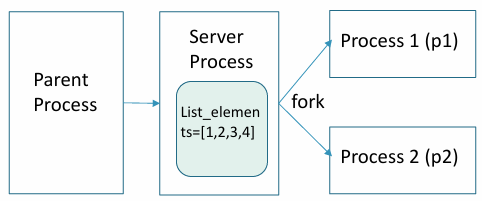
\includegraphics[width=0.45\textwidth]{figuresP/lesson_parallel_2B_pag_13}
\end{center}

\begin{Verbatim}[label=\makebox{\url{https://github.com/lucabaldini/cmepda/tree/master/slides/latex/snippets/multiprocessing_manager.py}},commandchars=\\\{\}]
\PY{k}{import} \PY{n+nn}{multiprocessing}

\PY{k}{def} \PY{n+nf}{add\PYZus{}element}\PY{p}{(}\PY{n}{record}\PY{p}{,}\PY{n}{records}\PY{p}{)}\PY{p}{:}
    \PY{n}{records}\PY{o}{.}\PY{n}{append}\PY{p}{(}\PY{n}{record}\PY{p}{)}
    \PY{n+nb}{print}\PY{p}{(}\PY{l+s+s2}{\PYZdq{}}\PY{l+s+s2}{New element added to records list}\PY{l+s+s2}{\PYZdq{}}\PY{p}{)}

\PY{k}{def} \PY{n+nf}{sum\PYZus{}elements}\PY{p}{(}\PY{n}{records}\PY{p}{)}\PY{p}{:}
    \PY{n}{summ}\PY{o}{=}\PY{n+nb}{sum}\PY{p}{(}\PY{n}{records}\PY{p}{)}
    \PY{n+nb}{print}\PY{p}{(}\PY{l+s+s2}{\PYZdq{}}\PY{l+s+s2}{New sum is: }\PY{l+s+s2}{\PYZdq{}}\PY{o}{+}\PY{n+nb}{str}\PY{p}{(}\PY{n}{summ}\PY{p}{)}\PY{p}{)}

\PY{c+c1}{\#MAIN}
\PY{k}{if} \PY{n}{\PYZus{}\PYZus{}name\PYZus{}\PYZus{}} \PY{o}{==} \PY{l+s+s1}{\PYZsq{}}\PY{l+s+s1}{\PYZus{}\PYZus{}main\PYZus{}\PYZus{}}\PY{l+s+s1}{\PYZsq{}}\PY{p}{:}
    \PY{c+c1}{\# Defining the manager (or server process)}
    \PY{k}{with} \PY{n}{multiprocessing}\PY{o}{.}\PY{n}{Manager}\PY{p}{(}\PY{p}{)} \PY{k}{as} \PY{n}{manager}\PY{p}{:}
        \PY{n}{list\PYZus{}elements}\PY{o}{=}\PY{p}{[}\PY{l+m+mi}{1}\PY{p}{,}\PY{l+m+mi}{2}\PY{p}{,}\PY{l+m+mi}{3}\PY{p}{,}\PY{l+m+mi}{4}\PY{p}{]}
        \PY{c+c1}{\# Here the list becomes \PYZdq{}usable\PYZdq{} for all the processes managed by the manager}
        \PY{n}{records}\PY{o}{=}\PY{n}{manager}\PY{o}{.}\PY{n}{list}\PY{p}{(}\PY{n}{list\PYZus{}elements}\PY{p}{)}
        \PY{n}{new\PYZus{}element}\PY{o}{=}\PY{l+m+mi}{5}

        \PY{n+nb}{print}\PY{p}{(}\PY{l+s+s2}{\PYZdq{}}\PY{l+s+s2}{Old sum is: }\PY{l+s+s2}{\PYZdq{}}\PY{o}{+}\PY{n+nb}{str}\PY{p}{(}\PY{n+nb}{sum}\PY{p}{(}\PY{n}{list\PYZus{}elements}\PY{p}{)}\PY{p}{)}\PY{p}{)}
        \PY{c+c1}{\# Creating new processes}
        \PY{n}{p1} \PY{o}{=} \PY{n}{multiprocessing}\PY{o}{.}\PY{n}{Process}\PY{p}{(}\PY{n}{target}\PY{o}{=}\PY{n}{add\PYZus{}element}\PY{p}{,} \PY{n}{args}\PY{o}{=}\PY{p}{(}\PY{n}{new\PYZus{}element}\PY{p}{,}\PY{n}{records}\PY{p}{)}\PY{p}{)}
        \PY{n}{p2} \PY{o}{=} \PY{n}{multiprocessing}\PY{o}{.}\PY{n}{Process}\PY{p}{(}\PY{n}{target}\PY{o}{=}\PY{n}{sum\PYZus{}elements}\PY{p}{,} \PY{n}{args}\PY{o}{=}\PY{p}{(}\PY{n}{records}\PY{p}{,}\PY{p}{)}\PY{p}{)}

        \PY{c+c1}{\# Running process p1 to insert new element}
        \PY{n}{p1}\PY{o}{.}\PY{n}{start}\PY{p}{(}\PY{p}{)}
        \PY{n}{p1}\PY{o}{.}\PY{n}{join}\PY{p}{(}\PY{p}{)}

        \PY{c+c1}{\# Running process p2 to sum list elements}
        \PY{n}{p2}\PY{o}{.}\PY{n}{start}\PY{p}{(}\PY{p}{)}
        \PY{n}{p2}\PY{o}{.}\PY{n}{join}\PY{p}{(}\PY{p}{)}

[Output]
Old sum is: 10
New element added to records list
New sum is: 15
\end{Verbatim}

\subsubsection{- Queue}

A simple way to communicate between processes with \texttt{multiprocessing} is to use a \textbf{queue} to pass messages back and forth. Any Python object can pass through a \texttt{multiprocessing.Queue()} object. Processes called \textit{producers} write something in the queue (\texttt{Queue.put()}), while the \textit{consumers} are the ones that read data from it. Here's an example:

\begin{center}
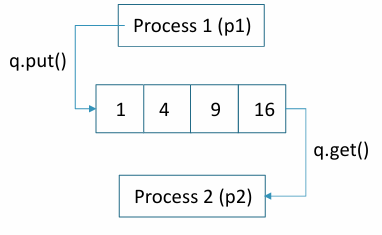
\includegraphics[width=0.4\textwidth]{figuresP/lesson_parallel_2B_pag_14}
\end{center}

\begin{Verbatim}[label=\makebox{\url{https://github.com/lucabaldini/cmepda/tree/master/slides/latex/snippets/multiprocessing_queue_passing.py}},commandchars=\\\{\}]
\PY{k}{import} \PY{n+nn}{multiprocessing}

\PY{k}{def} \PY{n+nf}{square\_list}\PY{p}{(}\PY{n}{mylist}\PY{p}{,} \PY{n}{q}\PY{p}{)}\PY{p}{:}
    \PY{c+c1}{\# Append squares of mylist to queue}
    \PY{k}{for} \PY{n}{num} \PY{k}{in} \PY{n}{mylist}\PY{p}{:}
        \PY{n}{q}\PY{o}{.}\PY{n}{put}\PY{p}{(}\PY{n}{num} \PY{o}{*} \PY{n}{num}\PY{p}{)}

\PY{k}{def} \PY{n+nf}{print\_queue}\PY{p}{(}\PY{n}{q}\PY{p}{)}\PY{p}{:}
    \PY{c+c1}{\# Function to print the elements in the Queue and empty it}
    \PY{n+nb}{print}\PY{p}{(}\PY{l+s+s2}{\PYZdq{}}\PY{l+s+s2}{Queue elements:}\PY{l+s+s2}{\PYZdq{}}\PY{p}{)}
    \PY{k}{while} \PY{o}{not} \PY{n}{q}\PY{o}{.}\PY{n}{empty}\PY{p}{(}\PY{p}{)}\PY{p}{:}
        \PY{n+nb}{print}\PY{p}{(}\PY{n}{q}\PY{o}{.}\PY{n}{get}\PY{p}{(}\PY{p}{)}\PY{p}{)}
    \PY{n+nb}{print}\PY{p}{(}\PY{l+s+s2}{\PYZdq{}}\PY{l+s+s2}{Queue is now empty!}\PY{l+s+s2}{\PYZdq{}}\PY{p}{)}

\PY{c+c1}{\#MAIN}
\PY{k}{if} \PY{n}{\_\_name\_\_}\PY{o}{==}\PY{l+s+s2}{\PYZdq{}}\PY{l+s+s2}{\_\_main\_\_}\PY{l+s+s2}{\PYZdq{}}\PY{p}{:}
    \PY{c+c1}{\# Input list}
    \PY{n}{mylist} \PY{o}{=} \PY{p}{[}\PY{l+m+mi}{1}\PY{p}{,}\PY{l+m+mi}{2}\PY{p}{,}\PY{l+m+mi}{3}\PY{p}{,}\PY{l+m+mi}{4}\PY{p}{]}
    \PY{c+c1}{\# Creating multiprocessing.Queue}
    \PY{n}{q} \PY{o}{=} \PY{n}{multiprocessing}\PY{o}{.}\PY{n}{Queue}\PY{p}{(}\PY{p}{)}

    \PY{c+c1}{\# Creating new processes}
    \PY{n}{p1} \PY{o}{=} \PY{n}{multiprocessing}\PY{o}{.}\PY{n}{Process}\PY{p}{(}\PY{n}{target}\PY{o}{=}\PY{n}{square\_list}\PY{p}{,} \PY{n}{args}\PY{o}{=}\PY{p}{(}\PY{n}{mylist}\PY{p}{,} \PY{n}{q}\PY{p}{)}\PY{p}{)}
    \PY{n}{p2} \PY{o}{=} \PY{n}{multiprocessing}\PY{o}{.}\PY{n}{Process}\PY{p}{(}\PY{n}{target}\PY{o}{=}\PY{n}{print\_queue}\PY{p}{,} \PY{n}{args}\PY{o}{=}\PY{p}{(}\PY{n}{q}\PY{p}{,}\PY{p}{)}\PY{p}{)}

    \PY{c+c1}{\# Running process p1 to square list}
    \PY{n}{p1}\PY{o}{.}\PY{n}{start}\PY{p}{(}\PY{p}{)}
    \PY{n}{p1}\PY{o}{.}\PY{n}{join}\PY{p}{(}\PY{p}{)}
    \PY{c+c1}{\# Running process p2 to get queue elements}
    \PY{n}{p2}\PY{o}{.}\PY{n}{start}\PY{p}{(}\PY{p}{)}
    \PY{n}{p2}\PY{o}{.}\PY{n}{join}\PY{p}{(}\PY{p}{)}

[Output]
Queue elements:
1
4
9
16
Queue is now empty!
\end{Verbatim}

\subsubsection{- Pipe}

A faster way to do practically the same thing is using a \textbf{pipe}. A pipe can have only two endpoints, hence it is preferred over a queue when only two-way communication is required. A queue is slower and it is built on top of a pipe. The \texttt{multiprocessing} module provides the \texttt{multiprocessing.Pipe()} class, which returns a pair of connection objects connected by a pipe (the two ends of the pipe itself). Each connection object has \texttt{send()} and \texttt{recv()} methods (among others), as shown in the following example.

\begin{center}
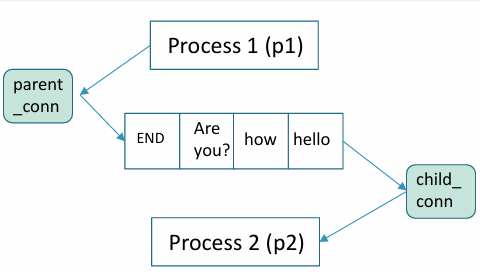
\includegraphics[width=0.4\textwidth]{figuresP/lesson_parallel_2B_pag_15}
\end{center}

\begin{Verbatim}[label=\makebox{\url{https://github.com/lucabaldini/cmepda/tree/master/slides/latex/snippets/multiprocessing_pipe.py}},commandchars=\\\{\}]
\PY{k}{import} \PY{n+nn}{multiprocessing}
\PY{k}{import} \PY{n+nn}{time}

\PY{k}{def} \PY{n+nf}{sender}\PY{p}{(}\PY{n}{conn}\PY{p}{,} \PY{n}{msgs}\PY{p}{)}\PY{p}{:}
    \PY{c+c1}{\# Function for the sender}
    \PY{k}{for} \PY{n}{msg} \PY{k}{in} \PY{n}{msgs}\PY{p}{:}
        \PY{n}{time}\PY{o}{.}\PY{n}{sleep}\PY{p}{(}\PY{l+m+mi}{1}\PY{p}{)}
        \PY{n}{conn}\PY{o}{.}\PY{n}{send}\PY{p}{(}\PY{n}{msg}\PY{p}{)}
        \PY{n+nb}{print}\PY{p}{(}\PY{l+s+s2}{\PYZdq{}}\PY{l+s+s2}{Sent the message: }\PY{l+s+s2}{\PYZdq{}}\PY{o}{+}\PY{n+nb}{str}\PY{p}{(}\PY{n}{msg}\PY{p}{)}\PY{p}{)}

    \PY{n}{conn}\PY{o}{.}\PY{n}{close}\PY{p}{(}\PY{p}{)}

\PY{k}{def} \PY{n+nf}{receiver}\PY{p}{(}\PY{n}{conn}\PY{p}{)}\PY{p}{:}
    \PY{c+c1}{\# Function for the receiver}
    \PY{n}{time}\PY{o}{.}\PY{n}{sleep}\PY{p}{(}\PY{l+m+mi}{2}\PY{p}{)}
    \PY{k}{while} \PY{l+m+mi}{1}\PY{p}{:}
        \PY{n}{msg} \PY{o}{=} \PY{n}{conn}\PY{o}{.}\PY{n}{recv}\PY{p}{(}\PY{p}{)}

        \PY{k}{if} \PY{n}{msg} \PY{o}{==} \PY{l+s+s2}{\PYZdq{}}\PY{l+s+s2}{END}\PY{l+s+s2}{\PYZdq{}}\PY{p}{:}
            \PY{k}{break}
        \PY{n+nb}{print}\PY{p}{(}\PY{l+s+s2}{\PYZdq{}}\PY{l+s+s2}{Received the message: }\PY{l+s+s2}{\PYZdq{}}\PY{o}{+}\PY{n+nb}{str}\PY{p}{(}\PY{n}{msg}\PY{p}{)}\PY{p}{)}

\PY{c+c1}{\#MAIN}
\PY{k}{if} \PY{n}{\_\_name\_\_}\PY{o}{==}\PY{l+s+s2}{\PYZdq{}}\PY{l+s+s2}{\_\_main\_\_}\PY{l+s+s2}{\PYZdq{}}\PY{p}{:}
    \PY{c+c1}{\# Messages to be sent}
    \PY{n}{msgs} \PY{o}{=} \PY{p}{[}\PY{l+s+s2}{\PYZdq{}}\PY{l+s+s2}{hello,}\PY{l+s+s2}{\PYZdq{}}\PY{p}{,} \PY{l+s+s2}{\PYZdq{}}\PY{l+s+s2}{how}\PY{l+s+s2}{\PYZdq{}}\PY{p}{,} \PY{l+s+s2}{\PYZdq{}}\PY{l+s+s2}{are you?}\PY{l+s+s2}{\PYZdq{}}\PY{p}{,} \PY{l+s+s2}{\PYZdq{}}\PY{l+s+s2}{END}\PY{l+s+s2}{\PYZdq{}}\PY{p}{]}
    \PY{c+c1}{\# Creating a pipe}
    \PY{n}{parent\PYZus{}conn}\PY{p}{,} \PY{n}{child\PYZus{}conn} \PY{o}{=} \PY{n}{multiprocessing}\PY{o}{.}\PY{n}{Pipe}\PY{p}{(}\PY{p}{)}

    \PY{c+c1}{\# Creating new processes}
    \PY{n}{p1} \PY{o}{=} \PY{n}{multiprocessing}\PY{o}{.}\PY{n}{Process}\PY{p}{(}\PY{n}{target}\PY{o}{=}\PY{n}{sender}\PY{p}{,} \PY{n}{args}\PY{o}{=}\PY{p}{(}\PY{n}{parent\PYZus{}conn}\PY{p}{,}\PY{n}{msgs}\PY{p}{)}\PY{p}{)}
    \PY{n}{p2} \PY{o}{=} \PY{n}{multiprocessing}\PY{o}{.}\PY{n}{Process}\PY{p}{(}\PY{n}{target}\PY{o}{=}\PY{n}{receiver}\PY{p}{,} \PY{n}{args}\PY{o}{=}\PY{p}{(}\PY{n}{child\PYZus{}conn}\PY{p}{,}\PY{p}{)}\PY{p}{)}

    \PY{c+c1}{\# Running processes}
    \PY{n}{p1}\PY{o}{.}\PY{n}{start}\PY{p}{(}\PY{p}{)}
    \PY{n}{p2}\PY{o}{.}\PY{n}{start}\PY{p}{(}\PY{p}{)}
    \PY{c+c1}{\# Wait until processes finish}
    \PY{n}{p1}\PY{o}{.}\PY{n}{join}\PY{p}{(}\PY{p}{)}
    \PY{n}{p2}\PY{o}{.}\PY{n}{join}\PY{p}{(}\PY{p}{)}

[Output]
Sent the message: hello,
Sent the message: how
Received the message: hello,
Received the message: how
Sent the message: are you?
Received the message: are you?
Sent the message: END
\end{Verbatim}

\subsection{Synchronization for processes: locking in Python}

\textbf{Process synchronization} is defined as a mechanism which ensures that two or more concurrent processes do not simultaneously execute some particular program segment known as \textbf{critical section}. A \textbf{race condition} occurs when two or more processes can access shared data and they try to change it at the same time. As a result, the values of variables may be unpredictable and vary depending on the timings of context switches of the processes.

Take a look at the following example. Here synchronization is not implemented and the results vary each time. It's a disaster!

\begin{Verbatim}[label=\makebox{\url{https://github.com/lucabaldini/cmepda/tree/master/slides/latex/snippets/synchro1.py}},commandchars=\\\{\}]
\PY{k}{import} \PY{n+nn}{multiprocessing}

\PY{k}{def} \PY{n+nf}{withdraw}\PY{p}{(}\PY{n}{balance}\PY{p}{)}\PY{p}{:}
    \PY{c+c1}{\# Function to withdraw from account}
    \PY{k}{for} \PY{n}{x} \PY{k}{in} \PY{n+nb}{range}\PY{p}{(}\PY{l+m+mi}{10000}\PY{p}{)}\PY{p}{:}
            \PY{n}{balance}\PY{o}{.}\PY{n}{value} \PY{o}{=} \PY{n}{balance}\PY{o}{.}\PY{n}{value}\PY{o}{\PYZhy{}}\PY{l+m+mi}{1}

\PY{k}{def} \PY{n+nf}{deposit}\PY{p}{(}\PY{n}{balance}\PY{p}{)}\PY{p}{:}
    \PY{c+c1}{\# Function to deposit in the account}
    \PY{k}{for} \PY{n}{x} \PY{k}{in} \PY{n+nb}{range}\PY{p}{(}\PY{l+m+mi}{10000}\PY{p}{)}\PY{p}{:}
        \PY{n}{balance}\PY{o}{.}\PY{n}{value} \PY{o}{=} \PY{n}{balance}\PY{o}{.}\PY{n}{value} \PY{o}{+} \PY{l+m+mi}{1}

\PY{k}{def} \PY{n+nf}{perform\PYZus{}transactions}\PY{p}{(}\PY{p}{)}\PY{p}{:}
    \PY{c+c1}{\# Initial balance (in shared memory) = 100\PYZdl{}}
    \PY{n}{balance} \PY{o}{=} \PY{n}{multiprocessing}\PY{o}{.}\PY{n}{Value}\PY{p}{(}\PY{l+s+s1}{\PYZsq{}}\PY{l+s+s1}{i}\PY{l+s+s1}{\PYZsq{}}\PY{p}{,} \PY{l+m+mi}{100}\PY{p}{)}
    \PY{c+c1}{\# Creating new processes}
    \PY{n}{p1} \PY{o}{=} \PY{n}{multiprocessing}\PY{o}{.}\PY{n}{Process}\PY{p}{(}\PY{n}{target}\PY{o}{=}\PY{n}{withdraw}\PY{p}{,} \PY{n}{args}\PY{o}{=}\PY{p}{(}\PY{n}{balance}\PY{p}{,}\PY{p}{)}\PY{p}{)}
    \PY{n}{p2} \PY{o}{=} \PY{n}{multiprocessing}\PY{o}{.}\PY{n}{Process}\PY{p}{(}\PY{n}{target}\PY{o}{=}\PY{n}{deposit}\PY{p}{,} \PY{n}{args}\PY{o}{=}\PY{p}{(}\PY{n}{balance}\PY{p}{,}\PY{p}{)}\PY{p}{)}
    \PY{c+c1}{\# Starting processes}
    \PY{n}{p1}\PY{o}{.}\PY{n}{start}\PY{p}{(}\PY{p}{)}
    \PY{n}{p2}\PY{o}{.}\PY{n}{start}\PY{p}{(}\PY{p}{)}
    \PY{c+c1}{\# Wait until processes are finished}
    \PY{n}{p1}\PY{o}{.}\PY{n}{join}\PY{p}{(}\PY{p}{)}
    \PY{n}{p2}\PY{o}{.}\PY{n}{join}\PY{p}{(}\PY{p}{)}
    \PY{c+c1}{\# Print final balance}
    \PY{n+nb}{print}\PY{p}{(}\PY{l+s+s2}{\PYZdq{}}\PY{l+s+s2}{Final balance = }\PY{l+s+si}{\PYZob{}\PYZcb{}}\PY{l+s+s2}{\PYZdq{}}\PY{o}{.}\PY{n}{format}\PY{p}{(}\PY{n}{balance}\PY{o}{.}\PY{n}{value}\PY{p}{)}\PY{p}{)}

\PY{c+c1}{\#MAIN}
\PY{k}{if} \PY{n}{\_\_name\_\_}\PY{o}{==}\PY{l+s+s2}{\PYZdq{}}\PY{l+s+s2}{\_\_main\_\_}\PY{l+s+s2}{\PYZdq{}}\PY{p}{:}
    \PY{k}{for} \PY{n}{x} \PY{k}{in} \PY{n+nb}{range}\PY{p}{(}\PY{l+m+mi}{10}\PY{p}{)}\PY{p}{:}
        \PY{c+c1}{\# Perform the same transaction process 10 times without syncrhonization}
        \PY{n}{perform\PYZus{}transactions}\PY{p}{(}\PY{p}{)}

[Output]
Final balance = 614
Final balance = -4609
Final balance = -176
Final balance = -1183
Final balance = 1896
Final balance = 138
Final balance = 699
Final balance = 2840
Final balance = -473
Final balance = -2117
\end{Verbatim}

The \texttt{multiprocessing} module provides a \texttt{Lock} class to deal with the race conditions, which is implemented using a Semaphore object provided by the OS, as shown below. As said, a semaphore is a synchronization object that controls access by multiple processes to a common resource in a parallel programming environment. It is simply a value in a designated place in the operating system (or kernel) storage that each process can check and then change. Depending on the value that is found, the process can use the resource or will find that it is already in use and must wait for some time before trying again.  

\begin{Verbatim}[label=\makebox{\url{https://github.com/lucabaldini/cmepda/tree/master/slides/latex/snippets/synchro2.py}},commandchars=\\\{\}]
\PY{k}{import} \PY{n+nn}{multiprocessing}

\PY{k}{def} \PY{n+nf}{withdraw}\PY{p}{(}\PY{n}{balance}\PY{p}{,} \PY{n}{lock}\PY{p}{)}\PY{p}{:}
    \PY{c+c1}{\# Function to withdraw from account}
    \PY{k}{for} \PY{n}{x} \PY{k}{in} \PY{n+nb}{range}\PY{p}{(}\PY{l+m+mi}{10000}\PY{p}{)}\PY{p}{:}
        \PY{c+c1}{\# Implementing a locking mechanism: syncrhonization}
        \PY{n}{lock}\PY{o}{.}\PY{n}{acquire}\PY{p}{(}\PY{p}{)}
        \PY{n}{balance}\PY{o}{.}\PY{n}{value} \PY{o}{=} \PY{n}{balance}\PY{o}{.}\PY{n}{value} \PY{o}{\PYZhy{}} \PY{l+m+mi}{1}
        \PY{n}{lock}\PY{o}{.}\PY{n}{release}\PY{p}{(}\PY{p}{)}

\PY{k}{def} \PY{n+nf}{deposit}\PY{p}{(}\PY{n}{balance}\PY{p}{,} \PY{n}{lock}\PY{p}{)}\PY{p}{:}
    \PY{c+c1}{\# Function to deposit to account}
    \PY{k}{for} \PY{n}{x} \PY{k}{in} \PY{n+nb}{range}\PY{p}{(}\PY{l+m+mi}{10000}\PY{p}{)}\PY{p}{:}
        \PY{c+c1}{\# Implementing a locking mechanism: syncrhonization}
        \PY{n}{lock}\PY{o}{.}\PY{n}{acquire}\PY{p}{(}\PY{p}{)}
        \PY{n}{balance}\PY{o}{.}\PY{n}{value} \PY{o}{=} \PY{n}{balance}\PY{o}{.}\PY{n}{value} \PY{o}{+} \PY{l+m+mi}{1}
        \PY{n}{lock}\PY{o}{.}\PY{n}{release}\PY{p}{(}\PY{p}{)}

\PY{k}{def} \PY{n+nf}{perform\PYZus{}transactions}\PY{p}{(}\PY{p}{)}\PY{p}{:}
    \PY{c+c1}{\# Initial balance (in shared memory)}
    \PY{n}{balance} \PY{o}{=} \PY{n}{multiprocessing}\PY{o}{.}\PY{n}{Value}\PY{p}{(}\PY{l+s+s1}{\PYZsq{}}\PY{l+s+s1}{i}\PY{l+s+s1}{\PYZsq{}}\PY{p}{,} \PY{l+m+mi}{100}\PY{p}{)}
    \PY{c+c1}{\# Creating a lock object}
    \PY{n}{lock} \PY{o}{=} \PY{n}{multiprocessing}\PY{o}{.}\PY{n}{Lock}\PY{p}{(}\PY{p}{)}

    \PY{c+c1}{\# Creating new processes}
    \PY{n}{p1} \PY{o}{=} \PY{n}{multiprocessing}\PY{o}{.}\PY{n}{Process}\PY{p}{(}\PY{n}{target}\PY{o}{=}\PY{n}{withdraw}\PY{p}{,} \PY{n}{args}\PY{o}{=}\PY{p}{(}\PY{n}{balance}\PY{p}{,}\PY{n}{lock}\PY{p}{)}\PY{p}{)}
    \PY{n}{p2} \PY{o}{=} \PY{n}{multiprocessing}\PY{o}{.}\PY{n}{Process}\PY{p}{(}\PY{n}{target}\PY{o}{=}\PY{n}{deposit}\PY{p}{,} \PY{n}{args}\PY{o}{=}\PY{p}{(}\PY{n}{balance}\PY{p}{,}\PY{n}{lock}\PY{p}{)}\PY{p}{)}
    \PY{c+c1}{\# Starting processes}
    \PY{n}{p1}\PY{o}{.}\PY{n}{start}\PY{p}{(}\PY{p}{)}
    \PY{n}{p2}\PY{o}{.}\PY{n}{start}\PY{p}{(}\PY{p}{)}
    \PY{c+c1}{\# Wait until processes are finished}
    \PY{n}{p1}\PY{o}{.}\PY{n}{join}\PY{p}{(}\PY{p}{)}
    \PY{n}{p2}\PY{o}{.}\PY{n}{join}\PY{p}{(}\PY{p}{)}

    \PY{c+c1}{\# Print final balance}
    \PY{n+nb}{print}\PY{p}{(}\PY{l+s+s2}{\PYZdq{}}\PY{l+s+s2}{Final balance = }\PY{l+s+s2}{\PYZdq{}}\PY{o}{+}\PY{n+nb}{str}\PY{p}{(}\PY{n}{balance}\PY{o}{.}\PY{n}{value}\PY{p}{)}\PY{p}{)}

\PY{c+c1}{\#MAIN}
\PY{k}{if} \PY{n}{\_\_name\_\_}\PY{o}{==}\PY{l+s+s2}{\PYZdq{}}\PY{l+s+s2}{\_\_main\_\_}\PY{l+s+s2}{\PYZdq{}}\PY{p}{:}
    \PY{k}{for} \PY{n}{x} \PY{k}{in} \PY{n+nb}{range}\PY{p}{(}\PY{l+m+mi}{10}\PY{p}{)}\PY{p}{:}
        \PY{c+c1}{\# Perform the same transaction process 10 times with syncrhonization}
        \PY{n}{perform\PYZus{}transactions}\PY{p}{(}\PY{p}{)}

[Output]
Final balance = 100
Final balance = 100
Final balance = 100
Final balance = 100
Final balance = 100
Final balance = 100
Final balance = 100
Final balance = 100
Final balance = 100
Final balance = 100
\end{Verbatim}

\subsection{Threading in Python} 


\begin{figure}[H]
\begin{minipage}{0.55\textwidth}
As said, multiple threads (which share the same global variables stored in the heap) can exist within one process, and each one of them contains its own register set and local variables (stored in the stack), as represented in figure.

\subsubsection{- The \texttt{threading} module}

Here's a simple example on how to define multiple threads using the \texttt{Thread} object in the \texttt{threading} module. Note that the syntax is very much similar to the \texttt{multiprocessing} module. First of all note that the PID of the process is the same for both threads, as expected. The following piece of code gives the impression that the threads \texttt{t1} and \texttt{t2} are running in parallel, but due to the GIL that's not the case. 

\end{minipage}\hfill
\begin{minipage}[c]{0.38\textwidth}
\centering
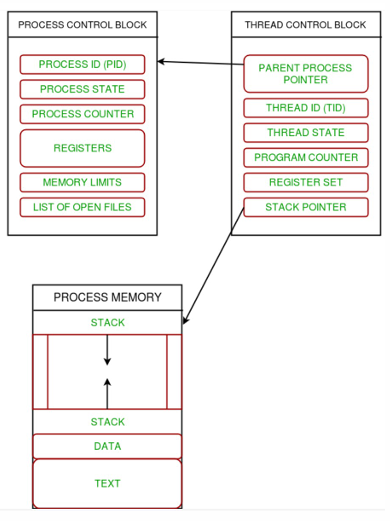
\includegraphics[width=\textwidth]{figuresP/lesson_parallel_2B_pag_18}
\end{minipage}
\end{figure}

%\begin{center}
%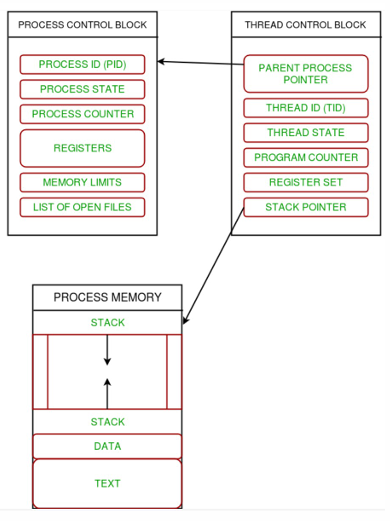
\includegraphics[width=0.3\textwidth]{figuresP/lesson_parallel_2B_pag_18}
%\end{center}

\begin{Verbatim}[label=\makebox{\url{https://github.com/lucabaldini/cmepda/tree/master/slides/latex/snippets/threading_basic.py}},commandchars=\\\{\}]
\PY{k}{import} \PY{n+nn}{threading}
\PY{k}{import} \PY{n+nn}{os}

\PY{k}{def} \PY{n+nf}{task1}\PY{p}{(}\PY{p}{)}\PY{p}{:}
        \PY{n+nb}{print}\PY{p}{(}\PY{l+s+s2}{\PYZdq{}}\PY{l+s+s2}{Task 1 assigned to thread: }\PY{l+s+s2}{\PYZdq{}}\PY{o}{+}\PY{n}{threading}\PY{o}{.}\PY{n}{current\PYZus{}thread}\PY{p}{(}\PY{p}{)}\PY{o}{.}\PY{n}{name}\PY{p}{)}
        \PY{n+nb}{print}\PY{p}{(}\PY{l+s+s2}{\PYZdq{}}\PY{l+s+s2}{ID of process running task 1: }\PY{l+s+s2}{\PYZdq{}}\PY{o}{+}\PY{n+nb}{str}\PY{p}{(}\PY{n}{os}\PY{o}{.}\PY{n}{getpid}\PY{p}{(}\PY{p}{)}\PY{p}{)}\PY{p}{)}
\PY{k}{def} \PY{n+nf}{task2}\PY{p}{(}\PY{p}{)}\PY{p}{:}
        \PY{n+nb}{print}\PY{p}{(}\PY{l+s+s2}{\PYZdq{}}\PY{l+s+s2}{Task 2 assigned to thread: }\PY{l+s+s2}{\PYZdq{}}\PY{o}{+}\PY{n}{threading}\PY{o}{.}\PY{n}{current\PYZus{}thread}\PY{p}{(}\PY{p}{)}\PY{o}{.}\PY{n}{name}\PY{p}{)}
        \PY{n+nb}{print}\PY{p}{(}\PY{l+s+s2}{\PYZdq{}}\PY{l+s+s2}{ID of process running task 2: }\PY{l+s+s2}{\PYZdq{}}\PY{o}{+}\PY{n+nb}{str}\PY{p}{(}\PY{n}{os}\PY{o}{.}\PY{n}{getpid}\PY{p}{(}\PY{p}{)}\PY{p}{)}\PY{p}{)}
\PY{c+c1}{\#MAIN}
\PY{k}{if} \PY{n}{\_\_name\_\_}\PY{o}{==}\PY{l+s+s2}{\PYZdq{}}\PY{l+s+s2}{\_\_main\_\_}\PY{l+s+s2}{\PYZdq{}}\PY{p}{:}
        \PY{c+c1}{\# Print ID of current process}
        \PY{n+nb}{print}\PY{p}{(}\PY{l+s+s2}{\PYZdq{}}\PY{l+s+s2}{ID of process running main program: }\PY{l+s+s2}{\PYZdq{}}\PY{o}{+}\PY{n+nb}{str}\PY{p}{(}\PY{n}{os}\PY{o}{.}\PY{n}{getpid}\PY{p}{(}\PY{p}{)}\PY{p}{)}\PY{p}{)}
        \PY{c+c1}{\# Print name of main thread}
        \PY{n+nb}{print}\PY{p}{(}\PY{l+s+s2}{\PYZdq{}}\PY{l+s+s2}{Main thread name: }\PY{l+s+s2}{\PYZdq{}}\PY{o}{+}\PY{n}{threading}\PY{o}{.}\PY{n}{main\PYZus{}thread}\PY{p}{(}\PY{p}{)}\PY{o}{.}\PY{n}{name}\PY{p}{)}

        \PY{c+c1}{\# Creating threads}
        \PY{n}{t1} \PY{o}{=} \PY{n}{threading}\PY{o}{.}\PY{n}{Thread}\PY{p}{(}\PY{n}{target}\PY{o}{=}\PY{n}{task1}\PY{p}{,} \PY{n}{name}\PY{o}{=}\PY{l+s+s1}{\PYZsq{}}\PY{l+s+s1}{t1}\PY{l+s+s1}{\PYZsq{}}\PY{p}{)}
        \PY{n}{t2} \PY{o}{=} \PY{n}{threading}\PY{o}{.}\PY{n}{Thread}\PY{p}{(}\PY{n}{target}\PY{o}{=}\PY{n}{task2}\PY{p}{,} \PY{n}{name}\PY{o}{=}\PY{l+s+s1}{\PYZsq{}}\PY{l+s+s1}{t2}\PY{l+s+s1}{\PYZsq{}}\PY{p}{)}
        \PY{c+c1}{\# Starting threads}
        \PY{n}{t1}\PY{o}{.}\PY{n}{start}\PY{p}{(}\PY{p}{)}
        \PY{n}{t2}\PY{o}{.}\PY{n}{start}\PY{p}{(}\PY{p}{)}
        \PY{c+c1}{\# Wait until all threads finish}
        \PY{n}{t1}\PY{o}{.}\PY{n}{join}\PY{p}{(}\PY{p}{)}
        \PY{n}{t2}\PY{o}{.}\PY{n}{join}\PY{p}{(}\PY{p}{)}

[Output]
ID of process running main program: 54321
Main thread name: MainThread
Task 1 assigned to thread: t1
ID of process running task 1: 54321
Task 2 assigned to thread: t2
ID of process running task 2: 54321
\end{Verbatim}

The following example shows how the GIL intervenes during code execution. Even though you should easily be able to see how a race condition should happen at runtime, the result is actually correct. That's the GIL's work: different threads are always executed at different times. 

\begin{Verbatim}[label=\makebox{\url{https://github.com/lucabaldini/cmepda/tree/master/slides/latex/snippets/threading_race_condition.py}},commandchars=\\\{\}]
\PY{k}{import} \PY{n+nn}{threading}

\PY{c+c1}{\# Global variable x}
\PY{n}{x} \PY{o}{=} \PY{l+m+mi}{0}

\PY{k}{def} \PY{n+nf}{increment}\PY{p}{(}\PY{p}{)}\PY{p}{:}
    \PY{k}{global} \PY{n}{x}
    \PY{n}{x} \PY{o}{+}\PY{o}{=} \PY{l+m+mi}{1}

\PY{k}{def} \PY{n+nf}{thread\_task}\PY{p}{(}\PY{p}{)}\PY{p}{:}
    \PY{k}{for} \PY{n}{\_} \PY{k}{in} \PY{n+nb}{range}\PY{p}{(}\PY{l+m+mi}{100000}\PY{p}{)}\PY{p}{:}
        \PY{n}{increment}\PY{p}{(}\PY{p}{)}

\PY{k}{def} \PY{n+nf}{main\_task}\PY{p}{(}\PY{p}{)}\PY{p}{:}
    \PY{k}{global} \PY{n}{x}
    \PY{c+c1}{\# Setting global variable x as 0}
    \PY{n}{x} \PY{o}{=} \PY{l+m+mi}{0}
    \PY{c+c1}{\# Creating threads}
    \PY{n}{t1} \PY{o}{=} \PY{n}{threading}\PY{o}{.}\PY{n}{Thread}\PY{p}{(}\PY{n}{target}\PY{o}{=}\PY{n}{thread\_task}\PY{p}{)}
    \PY{n}{t2} \PY{o}{=} \PY{n}{threading}\PY{o}{.}\PY{n}{Thread}\PY{p}{(}\PY{n}{target}\PY{o}{=}\PY{n}{thread\_task}\PY{p}{)}

    \PY{c+c1}{\# Start threads}
    \PY{n}{t1}\PY{o}{.}\PY{n}{start}\PY{p}{(}\PY{p}{)}
    \PY{n}{t2}\PY{o}{.}\PY{n}{start}\PY{p}{(}\PY{p}{)}
    \PY{c+c1}{\# Wait until threads finish their job}
    \PY{n}{t1}\PY{o}{.}\PY{n}{join}\PY{p}{(}\PY{p}{)}
    \PY{n}{t2}\PY{o}{.}\PY{n}{join}\PY{p}{(}\PY{p}{)}

\PY{c+c1}{\#MAIN}
\PY{k}{for} \PY{n}{i} \PY{k}{in} \PY{n+nb}{range}\PY{p}{(}\PY{l+m+mi}{10}\PY{p}{)}\PY{p}{:}
    \PY{n}{main\_task}\PY{p}{(}\PY{p}{)}
    \PY{n+nb}{print}\PY{p}{(}\PY{l+s+s2}{\PYZdq{}}\PY{l+s+s2}{Iteration }\PY{l+s+si}{\PYZob{}0\PYZcb{}}\PY{l+s+s2}{: x = }\PY{l+s+si}{\PYZob{}1\PYZcb{}}\PY{l+s+s2}{\PYZdq{}}\PY{o}{.}\PY{n}{format}\PY{p}{(}\PY{n}{i}\PY{p}{,}\PY{n}{x}\PY{p}{)}\PY{p}{)}

[Output]
Iteration 0: x = 200000
Iteration 1: x = 200000
Iteration 2: x = 200000
Iteration 3: x = 200000
Iteration 4: x = 200000
Iteration 5: x = 200000
Iteration 6: x = 200000
Iteration 7: x = 200000
Iteration 8: x = 200000
Iteration 9: x = 200000
\end{Verbatim}

However, it can be useful to implement a locking mechanism while using threading too. 

The GIL solves the problem of race conditions, but there may be some instances when you need a certain thread to run instead of another, even though they are acting on different data (e.g. one thread modifies an image, the other saves it in a folder: you need the first thread to finish before the second one does its job). 

Here's how you can implement synchronization using the \texttt{threading} module (the syntax is exactly the same as before):

\input{pygments/thread2b}

For further information on the \texttt{multiprocessing} and \texttt{threading} modules, take a look at the documentation: \\ - \texttt{multiprocessing}: \url{https://docs.python.org/3/library/multiprocessing.html}
\\ - \texttt{threading}: \url{https://docs.python.org/3/library/threading.html}.

\subsection{Comparison between threads and processes in Python}\label{sec:thread_process}

Lastly, we want to show the fundamental differences between code that utilizes threads and code that uses processes using a more complex example.

We want to write a program to factorize a list of 300 odd numbers between 1'000'000'001 and 1'000'000'597 and we want to measure the time needed to finish this operation using serial code, then 2, 4 or 8 threads and lastly 2, 4 or 8 processes. You can find the full code in Appendix \ref{app:final_example} and you can try to write it yourself. \\
Here's a graph with the result:

\begin{center}
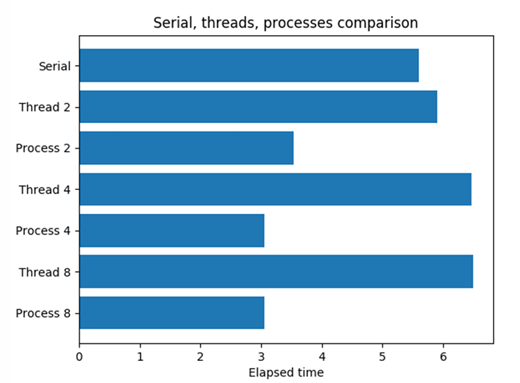
\includegraphics[width=0.6\textwidth]{figuresP/process_thread_comparison.png}
\end{center}

As you can see, the elapsed time with threads is always higher than the one obtained with serial execution. That is due to the GIL. With 2 processes we get a good speed-up, even though the elapsed time is not exactly halved due to the time needed by the OS to "organize" the execution. Moreover, note that with 4 processes we have already reached a saturation point due to Amdahl's law.

With that in mind, an important question is raised: why should I use threads? First of all, in case of I/O operations the GIL releases the lock (as previously said), so if your program needs to rapidly exchange large amounts of data, threads might be the way to go. More importantly (at least for calculus applications), if some of your functions are written in external C code, the GIL mechanism is bypassed and your threads will really be executed in parallel.

Here's another short recap:

\begin{center}
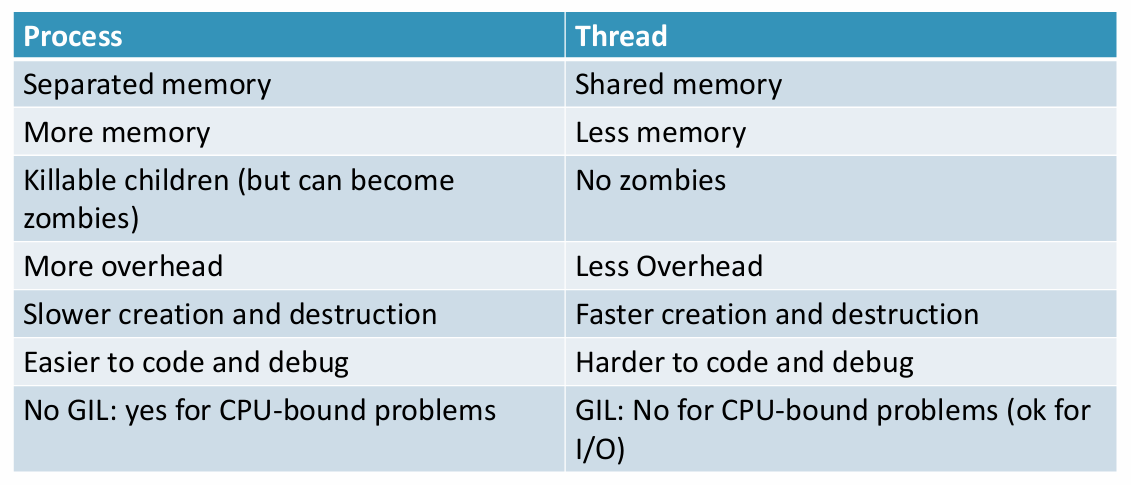
\includegraphics[width=0.7\textwidth]{figuresP/lesson_parallel_2B_pag_27}
\end{center}

A final thought for you: Python is really easy to use and understand, but these last sections should have shown you that it is not very efficient for parallelism. Fortran, C, C++ are better suited for that.

\underline{Final assignment}: Calculate for each number in a list the sum of all primes which are smaller than the given number. It should output the pairs [\texttt{n}, \texttt{sum\_primes(n)}] sorted by \texttt{n}. Example: If the input list is [10, 20], the expected output should be [[10, 17], [20, 77]]. Please use the \texttt{multiprocessing} module and compare the result (in terms of execution time) with the serial version of your code. Try to do the same with the \texttt{threading} module. Use big numbers like 2.5 million.
\section{A Short C Reminder for Python Programmers}

\footnote{I would like to thank Gemini Pro for the contribution it has given to writing this wonderful section. Thank you bro, we've come a long way together.} Minimal understanding of C syntax is strictly needed for the upcoming topics of this course. Since many of you are coming from a pure Python background, this section will serve as a bridge. Python is incredibly flexible, dynamic, and high-level, but when raw performance and direct hardware manipulation are required, such as in GPU computing, C is the absolute standard.

\subsection{Compiled vs Interpreted Languages}

The most fundamental difference between Python and C is how the computer executes them. Python is an \textbf{interpreted} language. When you run a script, the Python interpreter reads and executes the code line by line on the fly, either through an interactive shell or by running a \texttt{.py} file. 

C, on the other hand, is a \textbf{compiled} language. Before you can run a C program, you must pass the source code through a compiler (like \texttt{gcc}, \texttt{g++}, or \texttt{cc} on Linux). The compiler translates your entire human-readable code into a machine-executable binary file. 

This additional step makes development slightly slower, but the resulting execution is exponentially faster. Moreover, while Python reveals syntax errors only when it tries to execute the flawed line, the C compiler will catch all syntax errors beforehand, completely preventing compilation until they are fixed.

Let's now take a look at a simple program in C and go through with its execution.

\subsection{The anatomy of a basic C program}

Here it is: the classic "Hello World" program. 

\begin{Verbatim}[label=\makebox{\url{https://github.com/lucabaldini/cmepda/tree/master/slides/latex/snippets/hello_world.c}},commandchars=\\\{\}]
\PY{c+cp}{\#}\PY{c+cp}{include}\PY{+w}{ }\PY{c+cpf}{\PYZlt{}stdio.h\PYZgt{}}

\PY{k+kt}{int}\PY{+w}{ }\PY{n+nf}{main}\PY{p}{(}\PY{p}{)}\PY{+w}{ }\PY{p}{\PYZob{}}
\PY{+w}{    }\PY{c+cm}{/* my first program in C */}
\PY{+w}{    }\PY{n}{printf}\PY{p}{(}\PY{l+s}{\PYZdq{}}\PY{l+s}{Hello World! }\PY{l+s+se}{\PYZbs{}n}\PY{l+s}{\PYZdq{}}\PY{p}{)}\PY{p}{;}

\PY{+w}{    }\PY{k}{return}\PY{+w}{ }\PY{l+m+mi}{0}\PY{p}{;}
\PY{p}{\PYZcb{}}

[Output]
Hello World! 
\end{Verbatim}

Now, let's analyse this piece of code step by step so we can start understanding the C syntax. 
\begin{itemize}
    \item First of all, you must know that in Python, code can simply exist in the global scope, but in C code to be executed \textit{must} be enclosed within "functions". As an absolute minimum, every program must have a function called \textbf{\texttt{main}} (line 3)
    \item Python uses indentation to define blocks of code. In C, \textbf{blocks} of code instructions are enclosed in braces \textbf{\texttt{\{ \}}} (lines 3 and 8) and indentation is purely for human readability.
    \item Every single instruction (\textbf{statement}) must end with a semicolon \textbf{\texttt{;}} (line 7). Forgetting this is the most common cause of compiler errors.
    \item Text \textbf{strings} are enclosed by double quotes \textbf{\texttt{" "}} (line 5). Single quotes \texttt{' '} are strictly used for single characters only.
    \item Multi-line \textbf{comments} are enclosed by \textbf{\texttt{/* ... */}} (line 4). Single-line comments use {\texttt{/ /}} instead.
    \item You can include other pieces of code with the \texttt{\#include} directive (line 1). The \texttt{\#include <stdio.h>} line tells the compiler to include the \textit{Standard Input/Output library}, which is necessary to use the \texttt{printf} function. More generally, the word that comes after the \textbf{\texttt{\#}} symbol is called a \textbf{directive}, and, roughly speaking, it constitutes an "order" to the compiler (this concept will become clearer later).
    \item The \texttt{return 0} instruction (line 7) is not mandatory, but you will always find it for good practice at the end of each C program.
\end{itemize}

Now let's say that you have opened your favourite text editor and written the example program above in a file called \texttt{hello\_world.c} (the \texttt{.c} part is necessary, otherwise your compiler won't recognize the file). Let's also say that the file is saved in the directory \texttt{c/introduction\_to\_C}. If you are using Linux (as you should), in order to compile your file you must open the terminal, move inside the directory and then type \texttt{gcc hello\_world.c} (the same would be true on Windows). This will create an executable named \texttt{a.out} (or \texttt{a.exe} on Windows). In order to give it a more meaningful name, use the \texttt{-o} flag, just like this: \texttt{gcc hello\_world.c -o hello\_world} (on Windows you should type \texttt{gcc hello\_world.c -o hello\_world.exe}). \\ Once compiled, to run your program on Linux type \texttt{./hello\_world}. The \texttt{./} is mandatory as it tells the OS to look for the executable in the current directory (on Windows, you can simply type \texttt{hello\_world.exe} or just \texttt{hello\_world}). \footnote{Once you've become familiar with this process, you should consider switching to VS Code, which can hide all this operations for you and let you run C code just like a Python script.}

\subsection{Identifiers, Types and Variables}

Variables and functions names in C are called \textbf{identifiers}. An identifier must start with a letter or an underscore (not a number), and can then contain letters, numbers, and underscores. 

\begin{center}
    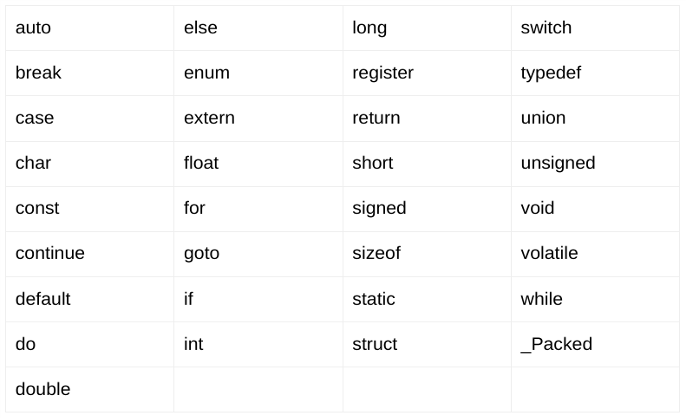
\includegraphics[width=0.65\textwidth]{figuresP/lesson_parallel_3a_pag_11.png}
\end{center}

Crucially, an identifier cannot be one of the reserved C \textbf{keywords} reported below.

\begin{center}
    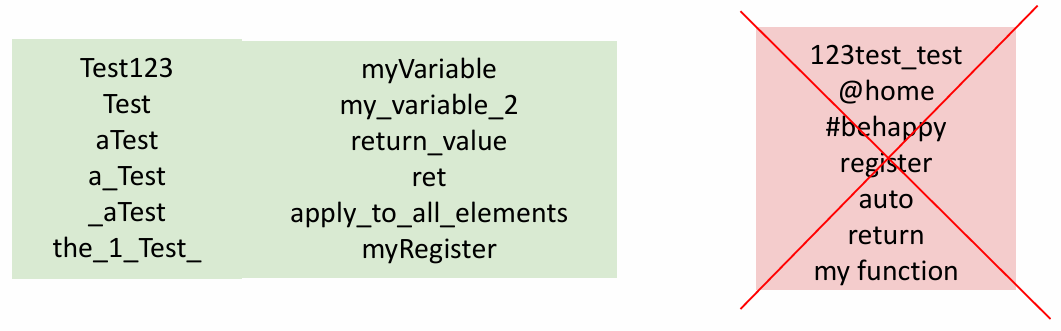
\includegraphics[width=0.65\textwidth]{figuresP/lesson_parallel_3a_pag_12.png}
\end{center}

Python is dynamically typed, while C is \textbf{statically typed}. That means that you must declare a variable type before using it through the syntax \texttt{type variablename;}. Here is a brief overview of the main variable types in C (you will find an example at the end of the list):

\subsubsection{- Integers and Floating Point numbers}

You can define integers and floating point numbers in many ways depending on your needs and your required precision, as shown in the following table.

\begin{table}[h]
\centering
\begin{tabular}{|c|c|c|c|}
\hline
\textbf{Type} & \textbf{Size (bits)} & \textbf{Size (bytes)} & \textbf{Range} \\
\hline
char & 8 & 1 & -128 to 127 \\
\hline
unsigned char & 8 & 1 & 0 to 255 \\
\hline
int & 16 & 2 & $-2^{15}$ to $2^{15}-1$ \\
\hline
unsigned int & 16 & 2 & 0 to $2^{16}-1$ \\
\hline
short int & 8 & 1 & -128 to 127 \\
\hline
unsigned short int & 8 & 1 & 0 to 255 \\
\hline
long int & 32 & 4 & $-2^{31}$ to $2^{31}-1$ \\
\hline
unsigned long int & 32 & 4 & 0 to $2^{32}-1$ \\
\hline
float & 32 & 4 & 3.4E-38 to 3.4E+38 \\
\hline
double & 64 & 8 & 1.7E-308 to 1.7E+308 \\
\hline
long double & 80 & 10 & 3.4E-4932 to 1.1E+4932 \\
\hline
\end{tabular}
\end{table}

Take a look at the different possible syntaxes for variable definition and printing methods in this example: 

\begin{Verbatim}[label=\makebox{\url{https://github.com/lucabaldini/cmepda/tree/master/slides/latex/snippets/variables_and_printf.c}},commandchars=\\\{\}]
\PY{c+cp}{\#}\PY{c+cp}{include}\PY{+w}{ }\PY{c+cpf}{\PYZlt{}stdio.h\PYZgt{}}
\PY{k+kt}{int}\PY{+w}{ }\PY{n+nf}{main}\PY{p}{(}\PY{p}{)}\PY{+w}{ }\PY{p}{\PYZob{}}
\PY{+w}{    }\PY{c+cm}{// Variable definition }
\PY{+w}{    }\PY{k+kt}{int}\PY{+w}{ }\PY{n}{a}\PY{p}{,}\PY{+w}{ }\PY{n}{b}\PY{p}{,}\PY{+w}{ }\PY{n}{c}\PY{p}{;}
\PY{+w}{    }\PY{n}{a}\PY{+w}{ }\PY{o}{=}\PY{+w}{ }\PY{l+m+mi}{2}\PY{p}{;}
\PY{+w}{    }\PY{n}{printf}\PY{p}{(}\PY{l+s}{\PYZdq{}}\PY{l+s}{a = \PYZpc{}d}\PY{l+s+se}{\PYZbs{}n}\PY{l+s}{\PYZdq{}}\PY{p}{,}\PY{+w}{ }\PY{n}{a}\PY{p}{)}\PY{p}{;}
\PY{+w}{    }\PY{k+kt}{int}\PY{+w}{ }\PY{n}{d}\PY{+w}{ }\PY{o}{=}\PY{+w}{ }\PY{l+m+mi}{1}\PY{p}{;}
\PY{+w}{    }\PY{k+kt}{float}\PY{+w}{ }\PY{n}{e}\PY{p}{;}
\PY{+w}{    }\PY{n}{e}\PY{+w}{ }\PY{o}{=}\PY{+w}{ }\PY{l+m+mf}{2.0}\PY{p}{;}
\PY{+w}{    }\PY{k+kt}{float}\PY{+w}{ }\PY{n}{f}\PY{+w}{ }\PY{o}{=}\PY{+w}{ }\PY{l+m+mf}{1.27}\PY{p}{;}
\PY{+w}{    }\PY{k+kt}{double}\PY{+w}{ }\PY{n}{g}\PY{+w}{ }\PY{o}{=}\PY{+w}{ }\PY{l+m+mf}{2.19293993847}\PY{p}{;}

\PY{+w}{    }\PY{n}{printf}\PY{p}{(}\PY{l+s}{\PYZdq{}}\PY{l+s}{e = \PYZpc{}d, }\PY{l+s}{\PYZdq{}}\PY{p}{,}\PY{+w}{ }\PY{n}{e}\PY{p}{)}\PY{p}{;}\PY{+w}{  }\PY{c+cm}{// Never pass a float and declare int !!!}
\PY{+w}{    }\PY{n}{printf}\PY{p}{(}\PY{l+s}{\PYZdq{}}\PY{l+s}{e = \PYZpc{}f, }\PY{l+s}{\PYZdq{}}\PY{p}{,}\PY{+w}{ }\PY{n}{e}\PY{p}{)}\PY{p}{;}
\PY{+w}{    }\PY{n}{printf}\PY{p}{(}\PY{l+s}{\PYZdq{}}\PY{l+s}{e = \PYZpc{}.1f}\PY{l+s+se}{\PYZbs{}n}\PY{l+s}{\PYZdq{}}\PY{p}{,}\PY{+w}{ }\PY{n}{e}\PY{p}{)}\PY{p}{;}

\PY{+w}{    }\PY{n}{printf}\PY{p}{(}\PY{l+s}{\PYZdq{}}\PY{l+s}{g = \PYZpc{}d, }\PY{l+s}{\PYZdq{}}\PY{p}{,}\PY{+w}{ }\PY{n}{g}\PY{p}{)}\PY{p}{;}\PY{+w}{  }\PY{c+cm}{// Never pass a float and declare int !!!}
\PY{+w}{    }\PY{n}{printf}\PY{p}{(}\PY{l+s}{\PYZdq{}}\PY{l+s}{g = \PYZpc{}f, }\PY{l+s}{\PYZdq{}}\PY{p}{,}\PY{+w}{ }\PY{n}{g}\PY{p}{)}\PY{p}{;}
\PY{+w}{    }\PY{n}{printf}\PY{p}{(}\PY{l+s}{\PYZdq{}}\PY{l+s}{g = \PYZpc{}.11f}\PY{l+s}{\PYZdq{}}\PY{p}{,}\PY{+w}{ }\PY{n}{g}\PY{p}{)}\PY{p}{;}

\PY{+w}{    }\PY{k}{return}\PY{+w}{ }\PY{l+m+mi}{0}\PY{p}{;}
\PY{p}{\PYZcb{}}

[Output]
a = 2
e = 0, e = 2.000000, e = 2.0
g = 405705013, g = 2.192940, g = 2.19293993847
\end{Verbatim}

\subsubsection{- Booleans}

Booleans are not defined in plain C. You must \texttt{\#include <stdbool.h>} to have the \texttt{bool} type defined. Otherwise, you can use the smallest integer (\texttt{char}) to represent them as 1 (true) and 0 (false).

\begin{Verbatim}[label=\makebox{\url{https://github.com/lucabaldini/cmepda/tree/master/slides/latex/snippets/booleans_in_c.c}},commandchars=\\\{\}]
\PY{c+cp}{\#}\PY{c+cp}{include}\PY{+w}{ }\PY{c+cpf}{\PYZlt{}stdio.h\PYZgt{}}
\PY{c+cp}{\#}\PY{c+cp}{include}\PY{+w}{ }\PY{c+cpf}{\PYZlt{}stdbool.h\PYZgt{}}\PY{c+c1}{ // Lets you use \PYZsq{}bool\PYZsq{}, \PYZsq{}true\PYZsq{} and \PYZsq{}false\PYZsq{}}

\PY{k+kt}{int}\PY{+w}{ }\PY{n+nf}{main}\PY{p}{(}\PY{p}{)}\PY{+w}{ }\PY{p}{\PYZob{}}
\PY{+w}{    }\PY{c+cm}{// Variable definition}
\PY{+w}{    }\PY{k+kt}{bool}\PY{+w}{ }\PY{n}{first\_method}\PY{+w}{ }\PY{o}{=}\PY{+w}{ }\PY{n+nb}{true}\PY{p}{;}
\PY{+w}{    }\PY{k+kt}{char}\PY{+w}{ }\PY{n}{second\_method}\PY{+w}{ }\PY{o}{=}\PY{+w}{ }\PY{l+m+mi}{1}\PY{p}{;}

\PY{+w}{    }\PY{n}{printf}\PY{p}{(}\PY{l+s}{\PYZdq{}}\PY{l+s}{bool (\PYZlt{}stdbool.h\PYZgt{}): \PYZpc{}d}\PY{l+s+se}{\PYZbs{}n}\PY{l+s}{\PYZdq{}}\PY{p}{,}\PY{+w}{ }\PY{n}{first\_method}\PY{p}{)}\PY{p}{;}
\PY{+w}{    }\PY{n}{printf}\PY{p}{(}\PY{l+s}{\PYZdq{}}\PY{l+s}{char (Plain C):     \PYZpc{}d}\PY{l+s+se}{\PYZbs{}n}\PY{l+s}{\PYZdq{}}\PY{p}{,}\PY{+w}{ }\PY{n}{second\_method}\PY{p}{)}\PY{p}{;}

\PY{+w}{    }\PY{k}{return}\PY{+w}{ }\PY{l+m+mi}{0}\PY{p}{;}
\PY{p}{\PYZcb{}}

[Output]
bool (<stdbool.h>): 1
char (Plain C):     1
\end{Verbatim}

\subsubsection{- Literals}

Constants or \textbf{literals} are fixed values explicitly defined in the code that cannot be modified during execution. In C, you can specify the exact type and base of a literal using specific prefixes and suffixes. This is particularly important because the compiler assigns default types to literals, which can affect the precision of mathematical operations.

\begin{itemize}
    \item[-] \textit{Integer literals:} They can be written in decimal, hexadecimal (using the \texttt{0x} prefix), or even octal format. You can append suffixes to specify their exact type: \texttt{U} or \texttt{u} for \texttt{unsigned}, and \texttt{L} or \texttt{l} for \texttt{long} (e.g., \texttt{1L}, \texttt{3U}).
    \item[-] \textit{Floating-point literals:} By default, any numerical literal with a decimal point is treated as a \texttt{double}. If you want to specify a \texttt{float}, you must append the \texttt{f} suffix (e.g., \texttt{1.f} or \texttt{3.14f}). For a \texttt{long double}, use the \texttt{L} suffix. You can also use \texttt{E} or \texttt{e} to indicate exponents in scientific notation.
\end{itemize}

Take a look at how different literal suffixes affect the precision and the result of a simple division in this example:

\begin{Verbatim}[label=\makebox{\url{https://github.com/lucabaldini/cmepda/tree/master/slides/latex/snippets/literals_and_precision.c}},commandchars=\\\{\}]
\PY{c+cp}{\#}\PY{c+cp}{include}\PY{+w}{ }\PY{c+cpf}{\PYZlt{}stdio.h\PYZgt{}}

\PY{k+kt}{int}\PY{+w}{ }\PY{n+nf}{main}\PY{p}{(}\PY{p}{)}\PY{+w}{ }\PY{p}{\PYZob{}}
\PY{+w}{    }\PY{c+c1}{// Integer Literals}
\PY{+w}{    }\PY{k+kt}{int}\PY{+w}{ }\PY{n}{dec}\PY{+w}{ }\PY{o}{=}\PY{+w}{ }\PY{l+m+mi}{42}\PY{p}{;}\PY{+w}{           }\PY{c+c1}{// Standard decimal}
\PY{+w}{    }\PY{k+kt}{int}\PY{+w}{ }\PY{n}{hex}\PY{+w}{ }\PY{o}{=}\PY{+w}{ }\PY{l+m+mh}{0x2A}\PY{p}{;}\PY{+w}{         }\PY{c+c1}{// Hexadecimal (0x prefix)}
\PY{+w}{    }\PY{k+kt}{int}\PY{+w}{ }\PY{n}{oct}\PY{+w}{ }\PY{o}{=}\PY{+w}{ }\PY{l+m+mo}{052}\PY{p}{;}\PY{+w}{          }\PY{c+c1}{// Octal (0 prefix)}
\PY{+w}{    }\PY{k+kt}{unsigned}\PY{+w}{ }\PY{k+kt}{int}\PY{+w}{ }\PY{n}{u}\PY{+w}{ }\PY{o}{=}\PY{+w}{ }\PY{l+m+mi}{42U}\PY{p}{;}\PY{+w}{   }\PY{c+c1}{// Unsigned (U or u suffix)}
\PY{+w}{    }\PY{k+kt}{long}\PY{+w}{ }\PY{k+kt}{int}\PY{+w}{ }\PY{n}{l}\PY{+w}{ }\PY{o}{=}\PY{+w}{ }\PY{l+m+mf}{42L}\PY{p}{;}\PY{+w}{       }\PY{c+c1}{// Long (L or l suffix)}

\PY{+w}{    }\PY{c+c1}{// Floating\PYZhy{}point Literals}
\PY{+w}{    }\PY{k+kt}{double}\PY{+w}{ }\PY{n}{d}\PY{+w}{ }\PY{o}{=}\PY{+w}{ }\PY{l+m+mf}{3.14}\PY{p}{;}\PY{+w}{        }\PY{c+c1}{// Double (Default)}
\PY{+w}{    }\PY{k+kt}{float}\PY{+w}{ }\PY{n}{f}\PY{+w}{ }\PY{o}{=}\PY{+w}{ }\PY{l+m+mf}{3.14f}\PY{p}{;}\PY{+w}{        }\PY{c+c1}{// Float (f or F suffix)}
\PY{+w}{    }\PY{k+kt}{long}\PY{+w}{ }\PY{k+kt}{double}\PY{+w}{ }\PY{n}{ld}\PY{+w}{ }\PY{o}{=}\PY{+w}{ }\PY{l+m+mf}{3.14L}\PY{p}{;}\PY{+w}{ }\PY{c+c1}{// Long double (L suffix)}
\PY{+w}{    }\PY{k+kt}{double}\PY{+w}{ }\PY{n}{sci}\PY{+w}{ }\PY{o}{=}\PY{+w}{ }\PY{l+m+mf}{3.14e\PYZhy{}2}\PY{p}{;}\PY{+w}{   }\PY{c+c1}{// Scientific notation (e or E exponent)}

\PY{+w}{    }\PY{c+c1}{// Precision Division Example}
\PY{+w}{    }\PY{c+c1}{// Demonstration of how suffixes affect the calculation}
\PY{+w}{    }\PY{k+kt}{long}\PY{+w}{ }\PY{k+kt}{double}\PY{+w}{ }\PY{n}{r}\PY{p}{;}

\PY{+w}{    }\PY{n}{r}\PY{+w}{ }\PY{o}{=}\PY{+w}{ }\PY{l+m+mi}{1}\PY{+w}{ }\PY{o}{/}\PY{+w}{ }\PY{l+m+mi}{3}\PY{p}{;}
\PY{+w}{    }\PY{n}{printf}\PY{p}{(}\PY{l+s}{\PYZdq{}}\PY{l+s}{1/3     (int)         = \PYZpc{}.30Lf}\PY{l+s+se}{\PYZbs{}n}\PY{l+s}{\PYZdq{}}\PY{p}{,}\PY{+w}{ }\PY{n}{r}\PY{p}{)}\PY{p}{;}
\PY{+w}{    }\PY{n}{r}\PY{+w}{ }\PY{o}{=}\PY{+w}{ }\PY{l+m+mf}{1.f}\PY{+w}{ }\PY{o}{/}\PY{+w}{ }\PY{l+m+mf}{3.f}\PY{p}{;}
\PY{+w}{    }\PY{n}{printf}\PY{p}{(}\PY{l+s}{\PYZdq{}}\PY{l+s}{1.f/3.f (float)       = \PYZpc{}.30Lf}\PY{l+s+se}{\PYZbs{}n}\PY{l+s}{\PYZdq{}}\PY{p}{,}\PY{+w}{ }\PY{n}{r}\PY{p}{)}\PY{p}{;}
\PY{+w}{    }\PY{n}{r}\PY{+w}{ }\PY{o}{=}\PY{+w}{ }\PY{l+m+mf}{1.}\PY{+w}{ }\PY{o}{/}\PY{+w}{ }\PY{l+m+mf}{3.}\PY{p}{;}
\PY{+w}{    }\PY{n}{printf}\PY{p}{(}\PY{l+s}{\PYZdq{}}\PY{l+s}{1./3.   (double)      = \PYZpc{}.30Lf}\PY{l+s+se}{\PYZbs{}n}\PY{l+s}{\PYZdq{}}\PY{p}{,}\PY{+w}{ }\PY{n}{r}\PY{p}{)}\PY{p}{;}
\PY{+w}{    }\PY{n}{r}\PY{+w}{ }\PY{o}{=}\PY{+w}{ }\PY{l+m+mf}{1.L}\PY{+w}{ }\PY{o}{/}\PY{+w}{ }\PY{l+m+mf}{3.L}\PY{p}{;}
\PY{+w}{    }\PY{n}{printf}\PY{p}{(}\PY{l+s}{\PYZdq{}}\PY{l+s}{1.L/3.L (long double) = \PYZpc{}.30Lf}\PY{l+s+se}{\PYZbs{}n}\PY{l+s}{\PYZdq{}}\PY{p}{,}\PY{+w}{ }\PY{n}{r}\PY{p}{)}\PY{p}{;}
\PY{+w}{    }\PY{n}{r}\PY{+w}{ }\PY{o}{=}\PY{+w}{ }\PY{l+m+mf}{1L}\PY{+w}{ }\PY{o}{/}\PY{+w}{ }\PY{l+m+mf}{3L}\PY{p}{;}
\PY{+w}{    }\PY{n}{printf}\PY{p}{(}\PY{l+s}{\PYZdq{}}\PY{l+s}{1L/3L   (long int)    = \PYZpc{}.30Lf}\PY{l+s+se}{\PYZbs{}n}\PY{l+s}{\PYZdq{}}\PY{p}{,}\PY{+w}{ }\PY{n}{r}\PY{p}{)}\PY{p}{;}
\PY{+w}{    }\PY{k}{return}\PY{+w}{ }\PY{l+m+mi}{0}\PY{p}{;}
\PY{p}{\PYZcb{}}

[Output]
1/3     (int)         = 0.000000000000000000000000000000
1.f/3.f (float)       = 0.333333343267440795898437500000
1./3.   (double)      = 0.333333333333333314829616256247
1.L/3.L (long double) = 0.333333333333333333342368351437
1L/3L   (long int)    = 0.000000000000000000000000000000
\end{Verbatim}

\hrulefill

\subsubsection{Note: Variables vs. Literals} 
The variables defined in the latter piece of code seem very similar to what we have seen in the paragraph about "Integers and Floating Point numbers", don't they? \\
It is essential to distinguish between variables and literals, which represent the container and the content, respectively. While data types (e.g., \texttt{int}, \texttt{float}) define the size and range of the memory \textit{containers} used to store data, literals are the raw, immutable \textit{values} written directly into the source code. For instance, in the statement \texttt{float f = 3.14f;}, \texttt{float f} allocates a 32-bit variable (the container), whereas \texttt{3.14f} is a float literal specifying that the hardcoded value must be interpreted explicitly as a float rather than the default double (the content).\\
That distinction must be perfectly clear!

\hrulefill

\subsection{Operators}

Now that you know how to declare variables, it is time to manipulate them. \textbf{Operators} in C share many similarities with Python, but there are a few fundamental distinctions, particularly concerning how true/false evaluations and bit-level operations are handled. Take a look at the examples after each paragraph to better understand these peculiarities. 

\subsubsection{- Math and Relational Operators}

Math operators in C implement standard arithmetic operations. Most of them are binary (e.g., \texttt{a + b}, \texttt{a * b}, \texttt{a \% b} for the modulo), but unary operators exist as well, such as the minus sign to negate a variable (\texttt{-a}).

Relational operators are used to compare two variables and are practically equivalent to their Python counterparts: \texttt{>}, \texttt{<}, \texttt{>=}, \texttt{<=}, \texttt{!=}, and \texttt{==}. Note that the operator to check if two variables have the same value is \texttt{==}, which must never be confused with the assignment operator \texttt{=}.

Since C originally lacked a native boolean type, relational operators return \texttt{1} for true and \texttt{0} for false. Furthermore, the unary logical NOT operator \texttt{!} considers \texttt{0} as false and any non-zero value as true. Consequently, negating a true value like 10 (\texttt{!10}) yields \texttt{0} (false). 

\begin{Verbatim}[label=\makebox{\url{https://github.com/lucabaldini/cmepda/tree/master/slides/latex/snippets/operators.c}},commandchars=\\\{\}]
\PY{c+cp}{\#}\PY{c+cp}{include}\PY{+w}{ }\PY{c+cpf}{\PYZlt{}stdio.h\PYZgt{}}
\PY{k+kt}{int}\PY{+w}{ }\PY{n+nf}{main}\PY{p}{(}\PY{p}{)}\PY{+w}{ }\PY{p}{\PYZob{}}
\PY{+w}{    }\PY{k+kt}{int}\PY{+w}{ }\PY{n}{a}\PY{+w}{ }\PY{o}{=}\PY{+w}{ }\PY{l+m+mi}{10}\PY{p}{;}
\PY{+w}{    }\PY{k+kt}{int}\PY{+w}{ }\PY{n}{b}\PY{+w}{ }\PY{o}{=}\PY{+w}{ }\PY{l+m+mi}{7}\PY{p}{;}

\PY{+w}{    }\PY{c+c1}{// Math operators}
\PY{+w}{    }\PY{n}{printf}\PY{p}{(}\PY{l+s}{\PYZdq{}}\PY{l+s}{a+b=\PYZpc{}d}\PY{l+s+se}{\PYZbs{}n}\PY{l+s}{\PYZdq{}}\PY{p}{,}\PY{+w}{ }\PY{n}{a}\PY{o}{+}\PY{n}{b}\PY{p}{)}\PY{p}{;}\PY{+w}{    }\PY{c+c1}{// a+b=17}
\PY{+w}{    }\PY{n}{printf}\PY{p}{(}\PY{l+s}{\PYZdq{}}\PY{l+s}{a\PYZhy{}b=\PYZpc{}d}\PY{l+s+se}{\PYZbs{}n}\PY{l+s}{\PYZdq{}}\PY{p}{,}\PY{+w}{ }\PY{n}{a}\PY{o}{\PYZhy{}}\PY{n}{b}\PY{p}{)}\PY{p}{;}\PY{+w}{    }\PY{c+c1}{// a\PYZhy{}b=3}
\PY{+w}{    }\PY{n}{printf}\PY{p}{(}\PY{l+s}{\PYZdq{}}\PY{l+s}{a*b=\PYZpc{}d}\PY{l+s+se}{\PYZbs{}n}\PY{l+s}{\PYZdq{}}\PY{p}{,}\PY{+w}{ }\PY{n}{a}\PY{o}{*}\PY{n}{b}\PY{p}{)}\PY{p}{;}\PY{+w}{    }\PY{c+c1}{// a*b=70}
\PY{+w}{    }\PY{n}{printf}\PY{p}{(}\PY{l+s}{\PYZdq{}}\PY{l+s}{a/b=\PYZpc{}d}\PY{l+s+se}{\PYZbs{}n}\PY{l+s}{\PYZdq{}}\PY{p}{,}\PY{+w}{ }\PY{n}{a}\PY{o}{/}\PY{n}{b}\PY{p}{)}\PY{p}{;}\PY{+w}{    }\PY{c+c1}{// a/b=1 (integer division!)}
\PY{+w}{    }\PY{n}{printf}\PY{p}{(}\PY{l+s}{\PYZdq{}}\PY{l+s}{a\PYZpc{}\PYZpc{}b=\PYZpc{}d}\PY{l+s+se}{\PYZbs{}n}\PY{l+s}{\PYZdq{}}\PY{p}{,}\PY{+w}{ }\PY{n}{a}\PY{o}{\PYZpc{}}\PY{n}{b}\PY{p}{)}\PY{p}{;}\PY{+w}{   }\PY{c+c1}{// a\PYZpc{}b=3}
\PY{+w}{    }\PY{n}{printf}\PY{p}{(}\PY{l+s}{\PYZdq{}}\PY{l+s}{\PYZhy{}a=\PYZpc{}d}\PY{l+s+se}{\PYZbs{}n}\PY{l+s}{\PYZdq{}}\PY{p}{,}\PY{+w}{ }\PY{o}{\PYZhy{}}\PY{n}{a}\PY{p}{)}\PY{p}{;}\PY{+w}{      }\PY{c+c1}{// \PYZhy{}a=\PYZhy{}10}
\PY{+w}{    }\PY{n}{printf}\PY{p}{(}\PY{l+s}{\PYZdq{}}\PY{l+s}{!a=\PYZpc{}d}\PY{l+s+se}{\PYZbs{}n}\PY{l+s}{\PYZdq{}}\PY{p}{,}\PY{+w}{ }\PY{o}{!}\PY{n}{a}\PY{p}{)}\PY{p}{;}\PY{+w}{      }\PY{c+c1}{// !a=0 (10 is true, so NOT 10 is false/0)}

\PY{+w}{    }\PY{c+c1}{// Relational operators}
\PY{+w}{    }\PY{n}{printf}\PY{p}{(}\PY{l+s}{\PYZdq{}}\PY{l+s}{a==b \PYZpc{}d}\PY{l+s+se}{\PYZbs{}n}\PY{l+s}{\PYZdq{}}\PY{p}{,}\PY{+w}{ }\PY{n}{a}\PY{o}{=}\PY{o}{=}\PY{n}{b}\PY{p}{)}\PY{p}{;}\PY{+w}{  }\PY{c+c1}{// a==b 0}
\PY{+w}{    }\PY{n}{printf}\PY{p}{(}\PY{l+s}{\PYZdq{}}\PY{l+s}{a!=b \PYZpc{}d}\PY{l+s+se}{\PYZbs{}n}\PY{l+s}{\PYZdq{}}\PY{p}{,}\PY{+w}{ }\PY{n}{a}\PY{o}{!}\PY{o}{=}\PY{n}{b}\PY{p}{)}\PY{p}{;}\PY{+w}{  }\PY{c+c1}{// a!=b 1}
\PY{+w}{    }\PY{n}{printf}\PY{p}{(}\PY{l+s}{\PYZdq{}}\PY{l+s}{a\PYZgt{}b  \PYZpc{}d}\PY{l+s+se}{\PYZbs{}n}\PY{l+s}{\PYZdq{}}\PY{p}{,}\PY{+w}{ }\PY{n}{a}\PY{o}{\PYZgt{}}\PY{n}{b}\PY{p}{)}\PY{p}{;}\PY{+w}{   }\PY{c+c1}{// a\PYZgt{}b 1}
\PY{+w}{    }\PY{n}{printf}\PY{p}{(}\PY{l+s}{\PYZdq{}}\PY{l+s}{a\PYZgt{}=b \PYZpc{}d}\PY{l+s+se}{\PYZbs{}n}\PY{l+s}{\PYZdq{}}\PY{p}{,}\PY{+w}{ }\PY{n}{a}\PY{o}{\PYZgt{}}\PY{o}{=}\PY{n}{b}\PY{p}{)}\PY{p}{;}\PY{+w}{  }\PY{c+c1}{// a\PYZgt{}=b 1}
\PY{+w}{    }\PY{n}{printf}\PY{p}{(}\PY{l+s}{\PYZdq{}}\PY{l+s}{a\PYZlt{}b  \PYZpc{}d}\PY{l+s+se}{\PYZbs{}n}\PY{l+s}{\PYZdq{}}\PY{p}{,}\PY{+w}{ }\PY{n}{a}\PY{o}{\PYZlt{}}\PY{n}{b}\PY{p}{)}\PY{p}{;}\PY{+w}{   }\PY{c+c1}{// a\PYZlt{}b 0}
\PY{+w}{    }\PY{n}{printf}\PY{p}{(}\PY{l+s}{\PYZdq{}}\PY{l+s}{a\PYZlt{}=b \PYZpc{}d}\PY{l+s+se}{\PYZbs{}n}\PY{l+s}{\PYZdq{}}\PY{p}{,}\PY{+w}{ }\PY{n}{a}\PY{o}{\PYZlt{}}\PY{o}{=}\PY{n}{b}\PY{p}{)}\PY{p}{;}\PY{+w}{  }\PY{c+c1}{// a\PYZlt{}=b 0}

\PY{+w}{    }\PY{k}{return}\PY{+w}{ }\PY{l+m+mi}{0}\PY{p}{;}
\PY{p}{\PYZcb{}}

[Output]
a+b=17
a-b=3
a*b=70
a/b=1
a%b=3
-a=-10
!a=0
a==b 0
a!=b 1
a>b  1
a>=b 1
a<b  0
a<=b 0
\end{Verbatim}

\subsubsection{- Logical vs Bitwise Operators}

In Python, you are used to writing \texttt{and}, \texttt{or}, and \texttt{not}. C introduces a strict separation between logical operations (which evaluate the overall truth of an expression) and bitwise operations (which act on the individual binary bits of the variables).

\begin{itemize}
    \item \textbf{Logical operators:} \texttt{\&\&} (AND), \texttt{||} (OR), and \texttt{!} (NOT). Just like in Python, they employ short-circuit evaluation: for example, the second operand in an OR expression is evaluated ONLY if the first one is false. They always return \texttt{0} or \texttt{1}.
    \item \textbf{Bitwise operators:} \texttt{\&} (AND), \texttt{|} (OR), \texttt{\^} (XOR), and \texttt{\~{}} (NOT). These act bit by bit. There are also the \texttt{>>} and \texttt{<<} operators, which shift the bits to the right or to the left, respectively.
\end{itemize}

\begin{Verbatim}[label=\makebox{\url{https://github.com/lucabaldini/cmepda/tree/master/slides/latex/snippets/bitwise_and_logical.c}},commandchars=\\\{\}]
\PY{c+cp}{\#}\PY{c+cp}{include}\PY{+w}{ }\PY{c+cpf}{\PYZlt{}stdio.h\PYZgt{}}

\PY{k+kt}{int}\PY{+w}{ }\PY{n+nf}{main}\PY{p}{(}\PY{p}{)}\PY{+w}{ }\PY{p}{\PYZob{}}
\PY{+w}{    }\PY{k+kt}{int}\PY{+w}{ }\PY{n}{a}\PY{+w}{ }\PY{o}{=}\PY{+w}{ }\PY{l+m+mi}{10}\PY{p}{;}\PY{+w}{  }\PY{c+c1}{// in binary: 00001010}
\PY{+w}{    }\PY{k+kt}{int}\PY{+w}{ }\PY{n}{b}\PY{+w}{ }\PY{o}{=}\PY{+w}{ }\PY{l+m+mi}{7}\PY{p}{;}\PY{+w}{   }\PY{c+c1}{// in binary: 00000111}

\PY{+w}{    }\PY{c+c1}{// Logical operators}
\PY{+w}{    }\PY{n}{printf}\PY{p}{(}\PY{l+s}{\PYZdq{}}\PY{l+s}{a \PYZam{}\PYZam{} b =\PYZgt{} \PYZpc{}d}\PY{l+s+se}{\PYZbs{}n}\PY{l+s}{\PYZdq{}}\PY{p}{,}\PY{+w}{ }\PY{n}{a}\PY{+w}{ }\PY{o}{\PYZam{}}\PY{o}{\PYZam{}}\PY{+w}{ }\PY{n}{b}\PY{p}{)}\PY{p}{;}\PY{+w}{ }\PY{c+c1}{// a AND b =\PYZgt{} 1}
\PY{+w}{    }\PY{n}{printf}\PY{p}{(}\PY{l+s}{\PYZdq{}}\PY{l+s}{a || b =\PYZgt{} \PYZpc{}d}\PY{l+s+se}{\PYZbs{}n}\PY{l+s}{\PYZdq{}}\PY{p}{,}\PY{+w}{ }\PY{n}{a}\PY{+w}{ }\PY{o}{|}\PY{o}{|}\PY{+w}{ }\PY{n}{b}\PY{p}{)}\PY{p}{;}\PY{+w}{ }\PY{c+c1}{// a OR b  =\PYZgt{} 1}
\PY{+w}{    }\PY{n}{printf}\PY{p}{(}\PY{l+s}{\PYZdq{}}\PY{l+s}{!a     =\PYZgt{} \PYZpc{}d}\PY{l+s+se}{\PYZbs{}n}\PY{l+s}{\PYZdq{}}\PY{p}{,}\PY{+w}{ }\PY{o}{!}\PY{n}{a}\PY{p}{)}\PY{p}{;}\PY{+w}{     }\PY{c+c1}{// NOT a   =\PYZgt{} 0}

\PY{+w}{    }\PY{c+c1}{// Bitwise operators}
\PY{+w}{    }\PY{n}{printf}\PY{p}{(}\PY{l+s}{\PYZdq{}}\PY{l+s}{a \PYZam{} b = \PYZpc{}d}\PY{l+s+se}{\PYZbs{}n}\PY{l+s}{\PYZdq{}}\PY{p}{,}\PY{+w}{ }\PY{n}{a}\PY{+w}{ }\PY{o}{\PYZam{}}\PY{+w}{ }\PY{n}{b}\PY{p}{)}\PY{p}{;}\PY{+w}{    }\PY{c+c1}{// 2    (00000010)}
\PY{+w}{    }\PY{n}{printf}\PY{p}{(}\PY{l+s}{\PYZdq{}}\PY{l+s}{a | b = \PYZpc{}d}\PY{l+s+se}{\PYZbs{}n}\PY{l+s}{\PYZdq{}}\PY{p}{,}\PY{+w}{ }\PY{n}{a}\PY{+w}{ }\PY{o}{|}\PY{+w}{ }\PY{n}{b}\PY{p}{)}\PY{p}{;}\PY{+w}{    }\PY{c+c1}{// 15   (00001111)}
\PY{+w}{    }\PY{n}{printf}\PY{p}{(}\PY{l+s}{\PYZdq{}}\PY{l+s}{a \PYZca{} b = \PYZpc{}d}\PY{l+s+se}{\PYZbs{}n}\PY{l+s}{\PYZdq{}}\PY{p}{,}\PY{+w}{ }\PY{n}{a}\PY{+w}{ }\PY{o}{\PYZca{}}\PY{+w}{ }\PY{n}{b}\PY{p}{)}\PY{p}{;}\PY{+w}{    }\PY{c+c1}{// 13   (00001101)}
\PY{+w}{    }\PY{n}{printf}\PY{p}{(}\PY{l+s}{\PYZdq{}}\PY{l+s}{\PYZti{}a    = \PYZpc{}d}\PY{l+s+se}{\PYZbs{}n}\PY{l+s}{\PYZdq{}}\PY{p}{,}\PY{+w}{ }\PY{o}{\PYZti{}}\PY{n}{a}\PY{p}{)}\PY{p}{;}\PY{+w}{       }\PY{c+c1}{// \PYZhy{}11  (11111111111111111111111111110101)}
\PY{+w}{    }\PY{n}{printf}\PY{p}{(}\PY{l+s}{\PYZdq{}}\PY{l+s}{a \PYZlt{}\PYZlt{} b = \PYZpc{}d}\PY{l+s+se}{\PYZbs{}n}\PY{l+s}{\PYZdq{}}\PY{p}{,}\PY{+w}{ }\PY{n}{a}\PY{+w}{ }\PY{o}{\PYZlt{}}\PY{o}{\PYZlt{}}\PY{+w}{ }\PY{n}{b}\PY{p}{)}\PY{p}{;}\PY{+w}{  }\PY{c+c1}{// 1280 (10100000000)}
\PY{+w}{    }\PY{n}{printf}\PY{p}{(}\PY{l+s}{\PYZdq{}}\PY{l+s}{a \PYZgt{}\PYZgt{} 1 = \PYZpc{}d}\PY{l+s+se}{\PYZbs{}n}\PY{l+s}{\PYZdq{}}\PY{p}{,}\PY{+w}{ }\PY{n}{a}\PY{+w}{ }\PY{o}{\PYZgt{}}\PY{o}{\PYZgt{}}\PY{+w}{ }\PY{l+m+mi}{1}\PY{p}{)}\PY{p}{;}\PY{+w}{  }\PY{c+c1}{// 5    (00000101)}

\PY{+w}{    }\PY{k}{return}\PY{+w}{ }\PY{l+m+mi}{0}\PY{p}{;}
\PY{p}{\PYZcb{}}

[Output]
a && b => 1
a || b => 1
!a     => 0
a & b = 2
a | b = 15
a ^ b = 13
~a    = -11
a << b = 1280
a >> 1 = 5
\end{Verbatim}

\subsubsection{- Assignment and Increment/Decrement Operators}

The assignment operator \texttt{=} changes the value of a variable. A peculiar feature of C is that the assignment operation itself returns the assigned value. For instance, the expression \texttt{c = (a = 3)} is perfectly valid and results in both \texttt{a} and \texttt{c} holding the value \texttt{3}.
Assignments can also be composed with binary operators (\texttt{+=}, \texttt{-=}, \texttt{>>=}, etc.), just like in Python.

A major novelty for Python programmers is the introduction of the increment (\texttt{++}) and decrement (\texttt{--}) operators. Their behavior changes drastically depending on their position relative to the variable:
\begin{itemize}
    \item \textbf{Postfixed} (e.g., \texttt{a++}): Returns the original value, then increments the variable.
    \item \textbf{Prefixed} (e.g., \texttt{++a}): Increments the variable first, then returns the new incremented value.
\end{itemize}

\begin{Verbatim}[label=\makebox{\url{https://github.com/lucabaldini/cmepda/tree/master/slides/latex/snippets/assignment_and_increment.c}},commandchars=\\\{\}]
\PY{c+cp}{\#}\PY{c+cp}{include}\PY{+w}{ }\PY{c+cpf}{\PYZlt{}stdio.h\PYZgt{}}

\PY{k+kt}{int}\PY{+w}{ }\PY{n+nf}{main}\PY{p}{(}\PY{p}{)}\PY{+w}{ }\PY{p}{\PYZob{}}
\PY{+w}{    }\PY{k+kt}{int}\PY{+w}{ }\PY{n}{a}\PY{+w}{ }\PY{o}{=}\PY{+w}{ }\PY{l+m+mi}{0}\PY{p}{;}
\PY{+w}{    }\PY{k+kt}{int}\PY{+w}{ }\PY{n}{b}\PY{+w}{ }\PY{o}{=}\PY{+w}{ }\PY{l+m+mi}{10}\PY{p}{;}

\PY{+w}{    }\PY{c+c1}{// Assignment operator}
\PY{+w}{    }\PY{n}{printf}\PY{p}{(}\PY{l+s}{\PYZdq{}}\PY{l+s}{\PYZpc{}d}\PY{l+s+se}{\PYZbs{}n}\PY{l+s}{\PYZdq{}}\PY{p}{,}\PY{+w}{ }\PY{n}{a}\PY{o}{=}\PY{n}{b}\PY{p}{)}\PY{p}{;}\PY{+w}{     }\PY{c+c1}{// 10 (assignment returns the assigned value)}
\PY{+w}{    }\PY{n}{printf}\PY{p}{(}\PY{l+s}{\PYZdq{}}\PY{l+s}{\PYZpc{}d}\PY{l+s+se}{\PYZbs{}n}\PY{l+s}{\PYZdq{}}\PY{p}{,}\PY{+w}{ }\PY{n}{b}\PY{o}{=}\PY{l+m+mi}{7}\PY{p}{)}\PY{p}{;}\PY{+w}{     }\PY{c+c1}{// 7}

\PY{+w}{    }\PY{c+c1}{// Composed assignment}
\PY{+w}{    }\PY{n}{a}\PY{+w}{ }\PY{o}{+}\PY{o}{=}\PY{+w}{ }\PY{n}{b}\PY{p}{;}\PY{+w}{                  }\PY{c+c1}{// a = a + b}
\PY{+w}{    }\PY{n}{printf}\PY{p}{(}\PY{l+s}{\PYZdq{}}\PY{l+s}{a+=b =\PYZgt{} \PYZpc{}d}\PY{l+s+se}{\PYZbs{}n}\PY{l+s}{\PYZdq{}}\PY{p}{,}\PY{+w}{ }\PY{n}{a}\PY{p}{)}\PY{p}{;}\PY{+w}{ }\PY{c+c1}{// 17}
\PY{+w}{    }\PY{n}{a}\PY{+w}{ }\PY{o}{\PYZhy{}}\PY{o}{=}\PY{+w}{ }\PY{n}{b}\PY{p}{;}\PY{+w}{                  }\PY{c+c1}{// a = a \PYZhy{} b}
\PY{+w}{    }\PY{n}{printf}\PY{p}{(}\PY{l+s}{\PYZdq{}}\PY{l+s}{a\PYZhy{}=b =\PYZgt{} \PYZpc{}d}\PY{l+s+se}{\PYZbs{}n}\PY{l+s}{\PYZdq{}}\PY{p}{,}\PY{+w}{ }\PY{n}{a}\PY{p}{)}\PY{p}{;}\PY{+w}{ }\PY{c+c1}{// 10}
\PY{+w}{    }\PY{n}{a}\PY{+w}{ }\PY{o}{\PYZgt{}}\PY{o}{\PYZgt{}}\PY{o}{=}\PY{+w}{ }\PY{l+m+mi}{2}\PY{p}{;}\PY{+w}{                 }\PY{c+c1}{// a = a \PYZgt{}\PYZgt{} 2}
\PY{+w}{    }\PY{n}{printf}\PY{p}{(}\PY{l+s}{\PYZdq{}}\PY{l+s}{a\PYZgt{}\PYZgt{}=2 =\PYZgt{} \PYZpc{}d}\PY{l+s+se}{\PYZbs{}n}\PY{l+s}{\PYZdq{}}\PY{p}{,}\PY{+w}{ }\PY{n}{a}\PY{p}{)}\PY{p}{;}\PY{+w}{ }\PY{c+c1}{// 2}

\PY{+w}{    }\PY{c+c1}{// Increment/Decrement operators}
\PY{+w}{    }\PY{n}{a}\PY{+w}{ }\PY{o}{=}\PY{+w}{ }\PY{l+m+mi}{10}\PY{p}{;}\PY{+w}{                  }\PY{c+c1}{// Resetting \PYZsq{}a\PYZsq{} to 10 for the next examples}

\PY{+w}{    }\PY{n}{printf}\PY{p}{(}\PY{l+s}{\PYZdq{}}\PY{l+s}{a++=\PYZpc{}d}\PY{l+s+se}{\PYZbs{}n}\PY{l+s}{\PYZdq{}}\PY{p}{,}\PY{+w}{ }\PY{n}{a}\PY{o}{+}\PY{o}{+}\PY{p}{)}\PY{p}{;}\PY{+w}{ }\PY{c+c1}{// a++=10 (returns original value, then a becomes 11)}
\PY{+w}{    }\PY{n}{printf}\PY{p}{(}\PY{l+s}{\PYZdq{}}\PY{l+s}{a=\PYZpc{}d}\PY{l+s+se}{\PYZbs{}n}\PY{l+s}{\PYZdq{}}\PY{p}{,}\PY{+w}{ }\PY{n}{a}\PY{p}{)}\PY{p}{;}\PY{+w}{     }\PY{c+c1}{// a=11}
\PY{+w}{    }\PY{n}{printf}\PY{p}{(}\PY{l+s}{\PYZdq{}}\PY{l+s}{a\PYZhy{}\PYZhy{}=\PYZpc{}d}\PY{l+s+se}{\PYZbs{}n}\PY{l+s}{\PYZdq{}}\PY{p}{,}\PY{+w}{ }\PY{n}{a}\PY{o}{\PYZhy{}}\PY{o}{\PYZhy{}}\PY{p}{)}\PY{p}{;}\PY{+w}{ }\PY{c+c1}{// a\PYZhy{}\PYZhy{}=11 (returns original value, then a becomes 10)}
\PY{+w}{    }\PY{n}{printf}\PY{p}{(}\PY{l+s}{\PYZdq{}}\PY{l+s}{a=\PYZpc{}d}\PY{l+s+se}{\PYZbs{}n}\PY{l+s}{\PYZdq{}}\PY{p}{,}\PY{+w}{ }\PY{n}{a}\PY{p}{)}\PY{p}{;}\PY{+w}{     }\PY{c+c1}{// a=10}

\PY{+w}{    }\PY{n}{printf}\PY{p}{(}\PY{l+s}{\PYZdq{}}\PY{l+s}{++a=\PYZpc{}d}\PY{l+s+se}{\PYZbs{}n}\PY{l+s}{\PYZdq{}}\PY{p}{,}\PY{+w}{ }\PY{o}{+}\PY{o}{+}\PY{n}{a}\PY{p}{)}\PY{p}{;}\PY{+w}{ }\PY{c+c1}{// ++a=11 (increments first, then returns new value)}
\PY{+w}{    }\PY{n}{printf}\PY{p}{(}\PY{l+s}{\PYZdq{}}\PY{l+s}{a=\PYZpc{}d}\PY{l+s+se}{\PYZbs{}n}\PY{l+s}{\PYZdq{}}\PY{p}{,}\PY{+w}{ }\PY{n}{a}\PY{p}{)}\PY{p}{;}\PY{+w}{     }\PY{c+c1}{// a=11}
\PY{+w}{    }\PY{n}{printf}\PY{p}{(}\PY{l+s}{\PYZdq{}}\PY{l+s}{\PYZhy{}\PYZhy{}a=\PYZpc{}d}\PY{l+s+se}{\PYZbs{}n}\PY{l+s}{\PYZdq{}}\PY{p}{,}\PY{+w}{ }\PY{o}{\PYZhy{}}\PY{o}{\PYZhy{}}\PY{n}{a}\PY{p}{)}\PY{p}{;}\PY{+w}{ }\PY{c+c1}{// \PYZhy{}\PYZhy{}a=10 (decrements first, then returns new value)}
\PY{+w}{    }\PY{n}{printf}\PY{p}{(}\PY{l+s}{\PYZdq{}}\PY{l+s}{a=\PYZpc{}d}\PY{l+s+se}{\PYZbs{}n}\PY{l+s}{\PYZdq{}}\PY{p}{,}\PY{+w}{ }\PY{n}{a}\PY{p}{)}\PY{p}{;}\PY{+w}{     }\PY{c+c1}{// a=10}

\PY{+w}{    }\PY{k}{return}\PY{+w}{ }\PY{l+m+mi}{0}\PY{p}{;}
\PY{p}{\PYZcb{}}

[Output]
10
7
a+=b => 17
a-=b => 10
a>>=2 => 2
a++=10
a=11
a--=11
a=10
++a=11
a=11
--a=10
a=10
\end{Verbatim}

\subsubsection{- Operator Precedence}

Just as algebraic rules dictate that multiplication precedes addition (\texttt{a + b * c} is obviously evaluated as \texttt{a + (b * c)}), C enforces a strict operator precedence. While standard math operations are intuitive, the precedence of bitwise, logical, and assignment operators can be tricky to remember. 
When in doubt, it is always a best practice to use parentheses \texttt{()} to explicitly define the execution order and make your code significantly more readable. The following table shows all the operators in order of precedence (from top to bottom).

\begin{center}
    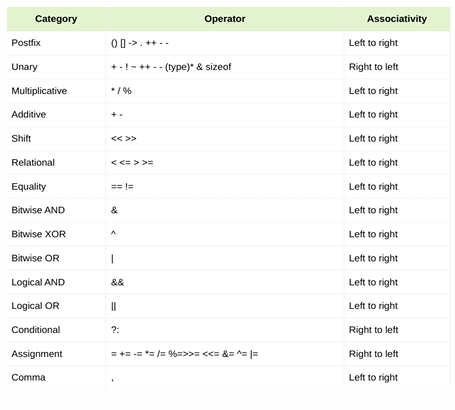
\includegraphics[width=0.65\textwidth]{figuresP/lesson_parallel_3a_pag_21.png}
\end{center}

\subsection{Control Flow and Output}

With operators at our disposal, we can now control the flow of our programs. If you are comfortable with Python, you will find C's control flow highly familiar in its logic, though noticeably different in its syntax. Let's explore conditional statements, loops, and how to properly print our results. As always, you should try and write for yourself the pieces of code at the end of each paragraph.

\subsubsection{- Conditional Statements: if, else, switch}

The fundamental \texttt{if/else} logic is practically identical to Python, but with two major syntax differences: conditions must be enclosed in parentheses \texttt{()}, and blocks of code are defined by braces \texttt{\{\}} instead of indentation. It is always a best practice to "protect" your \texttt{if} statements with braces even if they contain only a single line of code.

Crucially, C does not have an \texttt{elif} keyword. Instead, you simply chain them using \texttt{else if}.

C also provides two other ways to handle conditionals:
\begin{itemize}
    \item \textbf{The Ternary Operator (\texttt{?:}):} A compact, inline \texttt{if/else} statement. The syntax is \texttt{(expression) ? (return if true) : (return if false)}. It is the C equivalent of Python's \texttt{x if condition else y}.
    \item \textbf{The \texttt{switch/case} statement:} When you need to match a single variable against multiple constant values, a \texttt{switch} block is much cleaner than a long chain of \texttt{else if} statements. Remember to use the \texttt{break} keyword at the end of each \texttt{case}, otherwise the execution will "fall through" and execute the subsequent cases as well!
\end{itemize}

\begin{Verbatim}[label=\makebox{\url{https://github.com/lucabaldini/cmepda/tree/master/slides/latex/snippets/control_flow.c}},commandchars=\\\{\}]
\PY{c+cp}{\#}\PY{c+cp}{include}\PY{+w}{ }\PY{c+cpf}{\PYZlt{}stdio.h\PYZgt{}}

\PY{k+kt}{int}\PY{+w}{ }\PY{n+nf}{main}\PY{p}{(}\PY{p}{)}\PY{+w}{ }\PY{p}{\PYZob{}}
\PY{+w}{    }\PY{k+kt}{int}\PY{+w}{ }\PY{n}{a}\PY{+w}{ }\PY{o}{=}\PY{+w}{ }\PY{l+m+mi}{10}\PY{p}{;}
\PY{+w}{    }\PY{k+kt}{int}\PY{+w}{ }\PY{n}{b}\PY{+w}{ }\PY{o}{=}\PY{+w}{ }\PY{l+m+mi}{7}\PY{p}{;}

\PY{+w}{    }\PY{c+c1}{// if / else if / else}
\PY{+w}{    }\PY{k}{if}\PY{+w}{ }\PY{p}{(}\PY{n}{a}\PY{+w}{ }\PY{o}{=}\PY{o}{=}\PY{+w}{ }\PY{n}{b}\PY{p}{)}\PY{+w}{ }\PY{p}{\PYZob{}}
\PY{+w}{        }\PY{n}{printf}\PY{p}{(}\PY{l+s}{\PYZdq{}}\PY{l+s}{a and b are equal}\PY{l+s+se}{\PYZbs{}n}\PY{l+s}{\PYZdq{}}\PY{p}{)}\PY{p}{;}
\PY{+w}{    }\PY{p}{\PYZcb{}}\PY{+w}{ }\PY{k}{else}\PY{+w}{ }\PY{k}{if}\PY{+w}{ }\PY{p}{(}\PY{n}{a}\PY{+w}{ }\PY{o}{\PYZgt{}}\PY{+w}{ }\PY{n}{b}\PY{p}{)}\PY{+w}{ }\PY{p}{\PYZob{}}
\PY{+w}{        }\PY{n}{printf}\PY{p}{(}\PY{l+s}{\PYZdq{}}\PY{l+s}{a is greater}\PY{l+s+se}{\PYZbs{}n}\PY{l+s}{\PYZdq{}}\PY{p}{)}\PY{p}{;}
\PY{+w}{    }\PY{p}{\PYZcb{}}\PY{+w}{ }\PY{k}{else}\PY{+w}{ }\PY{p}{\PYZob{}}
\PY{+w}{        }\PY{n}{printf}\PY{p}{(}\PY{l+s}{\PYZdq{}}\PY{l+s}{b is greater}\PY{l+s+se}{\PYZbs{}n}\PY{l+s}{\PYZdq{}}\PY{p}{)}\PY{p}{;}
\PY{+w}{    }\PY{p}{\PYZcb{}}

\PY{+w}{    }\PY{c+c1}{// Ternary operator ?:}
\PY{+w}{    }\PY{n}{printf}\PY{p}{(}\PY{l+s}{\PYZdq{}}\PY{l+s}{a and b are }\PY{l+s}{\PYZdq{}}\PY{p}{)}\PY{p}{;}
\PY{+w}{    }\PY{n}{printf}\PY{p}{(}\PY{p}{(}\PY{n}{a}\PY{+w}{ }\PY{o}{=}\PY{o}{=}\PY{+w}{ }\PY{n}{b}\PY{p}{)}\PY{+w}{ }\PY{o}{?}\PY{+w}{ }\PY{l+s}{\PYZdq{}}\PY{l+s}{equal}\PY{l+s+se}{\PYZbs{}n}\PY{l+s}{\PYZdq{}}\PY{+w}{ }\PY{o}{:}\PY{+w}{ }\PY{l+s}{\PYZdq{}}\PY{l+s}{different}\PY{l+s+se}{\PYZbs{}n}\PY{l+s}{\PYZdq{}}\PY{p}{)}\PY{p}{;}

\PY{+w}{    }\PY{c+c1}{// Switch/case}
\PY{+w}{    }\PY{k+kt}{int}\PY{+w}{ }\PY{n}{choice}\PY{+w}{ }\PY{o}{=}\PY{+w}{ }\PY{l+m+mi}{2}\PY{p}{;}
\PY{+w}{    }\PY{k}{switch}\PY{+w}{ }\PY{p}{(}\PY{n}{choice}\PY{p}{)}\PY{+w}{ }\PY{p}{\PYZob{}}
\PY{+w}{        }\PY{k}{case}\PY{+w}{ }\PY{l+m+mi}{1}\PY{p}{:}
\PY{+w}{            }\PY{n}{printf}\PY{p}{(}\PY{l+s}{\PYZdq{}}\PY{l+s}{You chose 1}\PY{l+s+se}{\PYZbs{}n}\PY{l+s}{\PYZdq{}}\PY{p}{)}\PY{p}{;}
\PY{+w}{            }\PY{k}{break}\PY{p}{;}
\PY{+w}{        }\PY{k}{case}\PY{+w}{ }\PY{l+m+mi}{2}\PY{p}{:}
\PY{+w}{            }\PY{n}{printf}\PY{p}{(}\PY{l+s}{\PYZdq{}}\PY{l+s}{You chose 2}\PY{l+s+se}{\PYZbs{}n}\PY{l+s}{\PYZdq{}}\PY{p}{)}\PY{p}{;}
\PY{+w}{            }\PY{k}{break}\PY{p}{;}\PY{+w}{ }\PY{c+c1}{// Try removing this break to see the \PYZdq{}fall through\PYZdq{} effect!}
\PY{+w}{        }\PY{k}{default}\PY{o}{:}
\PY{+w}{            }\PY{n}{printf}\PY{p}{(}\PY{l+s}{\PYZdq{}}\PY{l+s}{Invalid choice}\PY{l+s+se}{\PYZbs{}n}\PY{l+s}{\PYZdq{}}\PY{p}{)}\PY{p}{;}
\PY{+w}{    }\PY{p}{\PYZcb{}}

\PY{+w}{    }\PY{k}{return}\PY{+w}{ }\PY{l+m+mi}{0}\PY{p}{;}
\PY{p}{\PYZcb{}}

[Output]
a is greater
a and b are different
You chose 2
\end{Verbatim}

\subsubsection{- The \texttt{printf} Function}

So far, we have used \texttt{printf} without properly introducing it. While Python's \texttt{print()} or f-strings automatically handle different data types, C requires you to explicitly declare the type of the variables you want to print using a \textbf{format string}.

Placeholders inside the string start with \texttt{\%} and are followed by a specific letter depending on the variable's type. The variables are then passed as subsequent arguments. Some of the most common specifiers include:
\begin{itemize}
    \item \texttt{\%d} or \texttt{\%i}: Decimal integer
    \item \texttt{\%f}: Floating point number
    \item \texttt{\%c}: Single character
    \item \texttt{\%s}: String of characters
\end{itemize}

Just like in Python, you can specify complex formatting, such as the number of decimal digits or leading zeroes (e.g., \texttt{\%.2f} for a float with two decimal places).

\begin{Verbatim}[label=\makebox{\url{https://github.com/lucabaldini/cmepda/tree/master/slides/latex/snippets/printf_formatting.c}},commandchars=\\\{\}]
\PY{c+cp}{\#}\PY{c+cp}{include}\PY{+w}{ }\PY{c+cpf}{\PYZlt{}stdio.h\PYZgt{}}

\PY{k+kt}{int}\PY{+w}{ }\PY{n+nf}{main}\PY{p}{(}\PY{p}{)}\PY{+w}{ }\PY{p}{\PYZob{}}
\PY{+w}{    }\PY{k+kt}{int}\PY{+w}{ }\PY{n}{age}\PY{+w}{ }\PY{o}{=}\PY{+w}{ }\PY{l+m+mi}{25}\PY{p}{;}
\PY{+w}{    }\PY{k+kt}{float}\PY{+w}{ }\PY{n}{pi}\PY{+w}{ }\PY{o}{=}\PY{+w}{ }\PY{l+m+mf}{3.14159f}\PY{p}{;}
\PY{+w}{    }\PY{k+kt}{char}\PY{+w}{ }\PY{n}{grade}\PY{+w}{ }\PY{o}{=}\PY{+w}{ }\PY{l+s+sc}{\PYZsq{}}\PY{l+s+sc}{A}\PY{l+s+sc}{\PYZsq{}}\PY{p}{;}

\PY{+w}{    }\PY{c+c1}{// Basic formatting}
\PY{+w}{    }\PY{n}{printf}\PY{p}{(}\PY{l+s}{\PYZdq{}}\PY{l+s}{I am \PYZpc{}d years old.}\PY{l+s+se}{\PYZbs{}n}\PY{l+s}{\PYZdq{}}\PY{p}{,}\PY{+w}{ }\PY{n}{age}\PY{p}{)}\PY{p}{;}
\PY{+w}{    }\PY{n}{printf}\PY{p}{(}\PY{l+s}{\PYZdq{}}\PY{l+s}{The value of pi is \PYZpc{}f.}\PY{l+s+se}{\PYZbs{}n}\PY{l+s}{\PYZdq{}}\PY{p}{,}\PY{+w}{ }\PY{n}{pi}\PY{p}{)}\PY{p}{;}
\PY{+w}{    }\PY{n}{printf}\PY{p}{(}\PY{l+s}{\PYZdq{}}\PY{l+s}{My grade is \PYZpc{}c.}\PY{l+s+se}{\PYZbs{}n}\PY{l+s}{\PYZdq{}}\PY{p}{,}\PY{+w}{ }\PY{n}{grade}\PY{p}{)}\PY{p}{;}

\PY{+w}{    }\PY{c+c1}{// Advanced formatting (precision and padding)}
\PY{+w}{    }\PY{n}{printf}\PY{p}{(}\PY{l+s}{\PYZdq{}}\PY{l+s}{Pi rounded to 2 decimals: \PYZpc{}.2f}\PY{l+s+se}{\PYZbs{}n}\PY{l+s}{\PYZdq{}}\PY{p}{,}\PY{+w}{ }\PY{n}{pi}\PY{p}{)}\PY{p}{;}
\PY{+w}{    }\PY{n}{printf}\PY{p}{(}\PY{l+s}{\PYZdq{}}\PY{l+s}{Padded integer: \PYZpc{}05d}\PY{l+s+se}{\PYZbs{}n}\PY{l+s}{\PYZdq{}}\PY{p}{,}\PY{+w}{ }\PY{n}{age}\PY{p}{)}\PY{p}{;}\PY{+w}{ }\PY{c+c1}{// Prints 00025}

\PY{+w}{    }\PY{c+c1}{// Multiple variables}
\PY{+w}{    }\PY{n}{printf}\PY{p}{(}\PY{l+s}{\PYZdq{}}\PY{l+s}{Values: \PYZpc{}d, \PYZpc{}.1f, \PYZpc{}c}\PY{l+s+se}{\PYZbs{}n}\PY{l+s}{\PYZdq{}}\PY{p}{,}\PY{+w}{ }\PY{n}{age}\PY{p}{,}\PY{+w}{ }\PY{n}{pi}\PY{p}{,}\PY{+w}{ }\PY{n}{grade}\PY{p}{)}\PY{p}{;}

\PY{+w}{    }\PY{k}{return}\PY{+w}{ }\PY{l+m+mi}{0}\PY{p}{;}
\PY{p}{\PYZcb{}}

[Output]
I am 25 years old.
The value of pi is 3.141590.
My grade is A.
Pi rounded to 2 decimals: 3.14
Padded integer: 00025
Values: 25, 3.1, A
\end{Verbatim}

\subsubsection{- Loops: for, while, do...while}

This is where Python programmers usually face a small learning curve. Python's \texttt{for} loop is actually a "for-each" loop, designed to iterate over collections (like lists or ranges). C's \texttt{for} loop, instead, is explicitly mechanical and controlled by three statements separated by semicolons: \texttt{for(initialization; condition; repeated action)}.
\begin{itemize}
    \item \textbf{Initialization:} Executed only once before the loop starts (e.g., \texttt{int i = 0}).
    \item \textbf{Condition:} Evaluated before every iteration. If true, the loop runs (e.g., \texttt{i < 10}).
    \item \textbf{Repeated action:} Executed at the end of every iteration (e.g., \texttt{i++}).
\end{itemize}

The \texttt{while} loop behaves exactly as it does in Python: it checks the condition \textit{before} the iteration starts.

C also introduces the \textbf{\texttt{do...while}} loop. The critical difference here is that the condition is checked \textit{after} the iteration. This guarantees that the code block inside a \texttt{do...while} loop is executed \textbf{at least once}, even if the condition is completely false from the very beginning.

Finally, the \texttt{break} (to exit the loop entirely) and \texttt{continue} (to skip the rest of the current iteration and proceed to the next) keywords work exactly as they do in Python.

\begin{Verbatim}[label=\makebox{\url{https://github.com/lucabaldini/cmepda/tree/master/slides/latex/snippets/loops.c}},commandchars=\\\{\}]
\PY{c+cp}{\#}\PY{c+cp}{include}\PY{+w}{ }\PY{c+cpf}{\PYZlt{}stdio.h\PYZgt{}}

\PY{k+kt}{int}\PY{+w}{ }\PY{n+nf}{main}\PY{p}{(}\PY{p}{)}\PY{+w}{ }\PY{p}{\PYZob{}}
\PY{+w}{    }\PY{c+c1}{// 1. FOR LOOP}
\PY{+w}{    }\PY{n}{printf}\PY{p}{(}\PY{l+s}{\PYZdq{}}\PY{l+s}{\PYZhy{}\PYZhy{}\PYZhy{} For Loop \PYZhy{}\PYZhy{}\PYZhy{}}\PY{l+s+se}{\PYZbs{}n}\PY{l+s}{\PYZdq{}}\PY{p}{)}\PY{p}{;}
\PY{+w}{    }\PY{k}{for}\PY{+w}{ }\PY{p}{(}\PY{k+kt}{int}\PY{+w}{ }\PY{n}{i}\PY{+w}{ }\PY{o}{=}\PY{+w}{ }\PY{l+m+mi}{0}\PY{p}{;}\PY{+w}{ }\PY{n}{i}\PY{+w}{ }\PY{o}{\PYZlt{}}\PY{+w}{ }\PY{l+m+mi}{3}\PY{p}{;}\PY{+w}{ }\PY{n}{i}\PY{o}{+}\PY{o}{+}\PY{p}{)}\PY{+w}{ }\PY{p}{\PYZob{}}
\PY{+w}{        }\PY{n}{printf}\PY{p}{(}\PY{l+s}{\PYZdq{}}\PY{l+s}{Iteration \PYZpc{}d}\PY{l+s+se}{\PYZbs{}n}\PY{l+s}{\PYZdq{}}\PY{p}{,}\PY{+w}{ }\PY{n}{i}\PY{p}{)}\PY{p}{;}
\PY{+w}{    }\PY{p}{\PYZcb{}}
\PY{+w}{    }
\PY{+w}{    }\PY{c+c1}{// 2. BREAK AND CONTINUE}
\PY{+w}{    }\PY{n}{printf}\PY{p}{(}\PY{l+s}{\PYZdq{}}\PY{l+s+se}{\PYZbs{}n}\PY{l+s}{\PYZhy{}\PYZhy{}\PYZhy{} Break \PYZam{} Continue \PYZhy{}\PYZhy{}\PYZhy{}}\PY{l+s+se}{\PYZbs{}n}\PY{l+s}{\PYZdq{}}\PY{p}{)}\PY{p}{;}
\PY{+w}{    }\PY{k}{for}\PY{+w}{ }\PY{p}{(}\PY{k+kt}{int}\PY{+w}{ }\PY{n}{i}\PY{+w}{ }\PY{o}{=}\PY{+w}{ }\PY{l+m+mi}{0}\PY{p}{;}\PY{+w}{ }\PY{n}{i}\PY{+w}{ }\PY{o}{\PYZlt{}}\PY{+w}{ }\PY{l+m+mi}{10}\PY{p}{;}\PY{+w}{ }\PY{n}{i}\PY{o}{+}\PY{o}{+}\PY{p}{)}\PY{+w}{ }\PY{p}{\PYZob{}}
\PY{+w}{        }\PY{k}{if}\PY{+w}{ }\PY{p}{(}\PY{n}{i}\PY{+w}{ }\PY{o}{\PYZgt{}}\PY{+w}{ }\PY{l+m+mi}{5}\PY{p}{)}\PY{+w}{ }\PY{k}{break}\PY{p}{;}\PY{+w}{       }\PY{c+c1}{// Exit loop if i \PYZgt{} 5}
\PY{+w}{        }\PY{k}{if}\PY{+w}{ }\PY{p}{(}\PY{n}{i}\PY{+w}{ }\PY{o}{\PYZgt{}}\PY{+w}{ }\PY{l+m+mi}{2}\PY{p}{)}\PY{+w}{ }\PY{k}{continue}\PY{p}{;}\PY{+w}{    }\PY{c+c1}{// Skip print if i \PYZgt{} 2 (but i \PYZlt{}= 5)}
\PY{+w}{        }\PY{n}{printf}\PY{p}{(}\PY{l+s}{\PYZdq{}}\PY{l+s}{Hi there, i is \PYZpc{}d}\PY{l+s+se}{\PYZbs{}n}\PY{l+s}{\PYZdq{}}\PY{p}{,}\PY{+w}{ }\PY{n}{i}\PY{p}{)}\PY{p}{;}\PY{+w}{ }
\PY{+w}{    }\PY{p}{\PYZcb{}}
\PY{+w}{    }
\PY{+w}{    }\PY{c+c1}{// 3. WHILE vs DO...WHILE}
\PY{+w}{    }\PY{n}{printf}\PY{p}{(}\PY{l+s}{\PYZdq{}}\PY{l+s+se}{\PYZbs{}n}\PY{l+s}{\PYZhy{}\PYZhy{}\PYZhy{} While vs Do...While \PYZhy{}\PYZhy{}\PYZhy{}}\PY{l+s+se}{\PYZbs{}n}\PY{l+s}{\PYZdq{}}\PY{p}{)}\PY{p}{;}
\PY{+w}{    }
\PY{+w}{    }\PY{k+kt}{int}\PY{+w}{ }\PY{n}{j}\PY{+w}{ }\PY{o}{=}\PY{+w}{ }\PY{l+m+mi}{0}\PY{p}{;}
\PY{+w}{    }\PY{k}{while}\PY{+w}{ }\PY{p}{(}\PY{n}{j}\PY{+w}{ }\PY{o}{\PYZlt{}}\PY{+w}{ }\PY{l+m+mi}{0}\PY{p}{)}\PY{+w}{ }\PY{p}{\PYZob{}}\PY{+w}{  }\PY{c+c1}{// Condition is false to start with!}
\PY{+w}{        }\PY{n}{j}\PY{o}{+}\PY{o}{+}\PY{p}{;}
\PY{+w}{        }\PY{n}{printf}\PY{p}{(}\PY{l+s}{\PYZdq{}}\PY{l+s}{while: j=\PYZpc{}d}\PY{l+s+se}{\PYZbs{}n}\PY{l+s}{\PYZdq{}}\PY{p}{,}\PY{+w}{ }\PY{n}{j}\PY{p}{)}\PY{p}{;}\PY{+w}{ }\PY{c+c1}{// This will never print}
\PY{+w}{    }\PY{p}{\PYZcb{}}
\PY{+w}{    }
\PY{+w}{    }\PY{k+kt}{int}\PY{+w}{ }\PY{n}{k}\PY{+w}{ }\PY{o}{=}\PY{+w}{ }\PY{l+m+mi}{0}\PY{p}{;}
\PY{+w}{    }\PY{k}{do}\PY{+w}{ }\PY{p}{\PYZob{}}\PY{+w}{             }\PY{c+c1}{// Condition is false, but executes once!}
\PY{+w}{        }\PY{n}{k}\PY{o}{+}\PY{o}{+}\PY{p}{;}
\PY{+w}{        }\PY{n}{printf}\PY{p}{(}\PY{l+s}{\PYZdq{}}\PY{l+s}{do...while: k=\PYZpc{}d}\PY{l+s+se}{\PYZbs{}n}\PY{l+s}{\PYZdq{}}\PY{p}{,}\PY{+w}{ }\PY{n}{k}\PY{p}{)}\PY{p}{;}\PY{+w}{ }
\PY{+w}{    }\PY{p}{\PYZcb{}}\PY{+w}{ }\PY{k}{while}\PY{+w}{ }\PY{p}{(}\PY{n}{k}\PY{+w}{ }\PY{o}{\PYZlt{}}\PY{+w}{ }\PY{l+m+mi}{0}\PY{p}{)}\PY{p}{;}
\PY{+w}{    }
\PY{+w}{    }\PY{n}{printf}\PY{p}{(}\PY{l+s}{\PYZdq{}}\PY{l+s}{After loops, j is \PYZpc{}d and k is \PYZpc{}d}\PY{l+s+se}{\PYZbs{}n}\PY{l+s}{\PYZdq{}}\PY{p}{,}\PY{+w}{ }\PY{n}{j}\PY{p}{,}\PY{+w}{ }\PY{n}{k}\PY{p}{)}\PY{p}{;}
\PY{+w}{    }
\PY{+w}{    }\PY{k}{return}\PY{+w}{ }\PY{l+m+mi}{0}\PY{p}{;}
\PY{p}{\PYZcb{}}

[Output]
--- For Loop ---
Iteration 0
Iteration 1
Iteration 2

--- Break & Continue ---
Hi there, i is 0
Hi there, i is 1
Hi there, i is 2

--- While vs Do...While ---
do...while: k=1
After loops, j is 0 and k is 1
\end{Verbatim}

\subsection{Functions and Scope}

In Python, defining a function is as simple as using the \texttt{def} keyword. In C, functions require a bit more structure. A C function consists of a \textbf{signature} (its name, the number of parameters, and their types) and a \textbf{body} (the actual code block). Furthermore, every function must specify a \textbf{return type}; if the function does not return anything, the type must be declared as \texttt{void}.

A crucial difference from Python is the distinction between \textbf{defining} and \textbf{declaring} a function:
\begin{itemize}
    \item \textbf{Defining:} Writing the full function, including its body.
    \item \textbf{Declaring:} Providing only the signature to the compiler, usually at the top of the file or in a header file.
\end{itemize}
Why declare? The C compiler reads code from top to bottom. If function A calls function B, function B must be known to the compiler beforehand. Declaring allows you to inform the compiler that a function exists and what it looks like, even if its actual definition is written further down in the file (or in a completely different file). This is essential for mutually recursive functions.

Another major difference is \textbf{variable scope}. While Python's scope is mostly tied to functions and modules, C uses \textbf{block scope}: variables strictly exist only within the block \texttt{\{\}} where they are declared. If you declare a variable inside a nested block with the same name as one outside of it, the inner variable will "hide" the outer one until the block ends. Here's an example:

\begin{Verbatim}[label=\makebox{\url{https://github.com/lucabaldini/cmepda/tree/master/slides/latex/snippets/functions_and_scope.c}},commandchars=\\\{\}]
\PY{c+cp}{\#}\PY{c+cp}{include}\PY{+w}{ }\PY{c+cpf}{\PYZlt{}stdio.h\PYZgt{}}
\PY{c+cp}{\#}\PY{c+cp}{include}\PY{+w}{ }\PY{c+cpf}{\PYZlt{}stdbool.h\PYZgt{}}

\PY{c+c1}{// 1. Declaration (providing the signature before definition)}
\PY{k+kt}{bool}\PY{+w}{ }\PY{n}{isEven}\PY{p}{(}\PY{k+kt}{int}\PY{+w}{ }\PY{n}{n}\PY{p}{)}\PY{p}{;}

\PY{c+c1}{// 2. Definition}
\PY{k+kt}{bool}\PY{+w}{ }\PY{n+nf}{isOdd}\PY{p}{(}\PY{k+kt}{int}\PY{+w}{ }\PY{n}{n}\PY{p}{)}\PY{+w}{ }\PY{p}{\PYZob{}}
\PY{+w}{    }\PY{k}{if}\PY{+w}{ }\PY{p}{(}\PY{n}{n}\PY{+w}{ }\PY{o}{=}\PY{o}{=}\PY{+w}{ }\PY{l+m+mi}{0}\PY{p}{)}\PY{+w}{ }\PY{k}{return}\PY{+w}{ }\PY{n+nb}{false}\PY{p}{;}
\PY{+w}{    }\PY{c+c1}{// Calls isEven, which the compiler knows about thanks to the declaration}
\PY{+w}{    }\PY{k}{return}\PY{+w}{ }\PY{n}{isEven}\PY{p}{(}\PY{n}{n}\PY{+w}{ }\PY{o}{\PYZhy{}}\PY{+w}{ }\PY{l+m+mi}{1}\PY{p}{)}\PY{p}{;}
\PY{p}{\PYZcb{}}

\PY{k+kt}{bool}\PY{+w}{ }\PY{n+nf}{isEven}\PY{p}{(}\PY{k+kt}{int}\PY{+w}{ }\PY{n}{n}\PY{p}{)}\PY{+w}{ }\PY{p}{\PYZob{}}
\PY{+w}{    }\PY{k}{if}\PY{+w}{ }\PY{p}{(}\PY{n}{n}\PY{+w}{ }\PY{o}{=}\PY{o}{=}\PY{+w}{ }\PY{l+m+mi}{0}\PY{p}{)}\PY{+w}{ }\PY{k}{return}\PY{+w}{ }\PY{n+nb}{true}\PY{p}{;}
\PY{+w}{    }\PY{k}{return}\PY{+w}{ }\PY{n}{isOdd}\PY{p}{(}\PY{n}{n}\PY{+w}{ }\PY{o}{\PYZhy{}}\PY{+w}{ }\PY{l+m+mi}{1}\PY{p}{)}\PY{p}{;}
\PY{p}{\PYZcb{}}

\PY{k+kt}{int}\PY{+w}{ }\PY{n+nf}{main}\PY{p}{(}\PY{p}{)}\PY{+w}{ }\PY{p}{\PYZob{}}
\PY{+w}{    }\PY{k+kt}{int}\PY{+w}{ }\PY{n}{a}\PY{+w}{ }\PY{o}{=}\PY{+w}{ }\PY{l+m+mi}{1}\PY{p}{;}
\PY{+w}{    }\PY{k+kt}{int}\PY{+w}{ }\PY{n}{b}\PY{+w}{ }\PY{o}{=}\PY{+w}{ }\PY{l+m+mi}{10}\PY{p}{;}
\PY{+w}{    }
\PY{+w}{    }\PY{c+c1}{// 3. Variable Scope}
\PY{+w}{    }\PY{p}{\PYZob{}}\PY{+w}{ }\PY{c+c1}{// Start of a new nested block}
\PY{+w}{        }\PY{k+kt}{int}\PY{+w}{ }\PY{n}{a}\PY{+w}{ }\PY{o}{=}\PY{+w}{ }\PY{l+m+mi}{100}\PY{p}{;}\PY{+w}{ }\PY{c+c1}{// This \PYZsq{}a\PYZsq{} hides the outer \PYZsq{}a\PYZsq{}}
\PY{+w}{        }\PY{k+kt}{int}\PY{+w}{ }\PY{n}{c}\PY{+w}{ }\PY{o}{=}\PY{+w}{ }\PY{l+m+mi}{10000}\PY{p}{;}
\PY{+w}{        }\PY{n}{printf}\PY{p}{(}\PY{l+s}{\PYZdq{}}\PY{l+s}{Inner block: a = \PYZpc{}d, b = \PYZpc{}d}\PY{l+s+se}{\PYZbs{}n}\PY{l+s}{\PYZdq{}}\PY{p}{,}\PY{+w}{ }\PY{n}{a}\PY{p}{,}\PY{+w}{ }\PY{n}{b}\PY{p}{)}\PY{p}{;}
\PY{+w}{    }\PY{p}{\PYZcb{}}\PY{+w}{ }\PY{c+c1}{// \PYZsq{}c\PYZsq{} is destroyed here, and the inner \PYZsq{}a\PYZsq{} is destroyed}
\PY{+w}{    }
\PY{+w}{    }\PY{n}{printf}\PY{p}{(}\PY{l+s}{\PYZdq{}}\PY{l+s}{Outer block: a = \PYZpc{}d}\PY{l+s+se}{\PYZbs{}n}\PY{l+s}{\PYZdq{}}\PY{p}{,}\PY{+w}{ }\PY{n}{a}\PY{p}{)}\PY{p}{;}
\PY{+w}{    }\PY{c+c1}{// printf(\PYZdq{}\PYZpc{}d\PYZdq{}, c); // This would cause a compile error: \PYZsq{}c\PYZsq{} undeclared}
\PY{+w}{    }
\PY{+w}{    }\PY{n}{printf}\PY{p}{(}\PY{l+s}{\PYZdq{}}\PY{l+s}{Is 17 even? \PYZpc{}s}\PY{l+s+se}{\PYZbs{}n}\PY{l+s}{\PYZdq{}}\PY{p}{,}\PY{+w}{ }\PY{n}{isEven}\PY{p}{(}\PY{l+m+mi}{17}\PY{p}{)}\PY{+w}{ }\PY{o}{?}\PY{+w}{ }\PY{l+s}{\PYZdq{}}\PY{l+s}{true}\PY{l+s}{\PYZdq{}}\PY{+w}{ }\PY{o}{:}\PY{+w}{ }\PY{l+s}{\PYZdq{}}\PY{l+s}{false}\PY{l+s}{\PYZdq{}}\PY{p}{)}\PY{p}{;}
\PY{+w}{    }
\PY{+w}{    }\PY{k}{return}\PY{+w}{ }\PY{l+m+mi}{0}\PY{p}{;}
\PY{p}{\PYZcb{}}

[Output]
Inner block: a = 100, b = 10
Outer block: a = 1
Is 17 even? false
\end{Verbatim}

\subsection{Variables, Memory, and Pointers}

To truly understand C, you must understand how it manages memory. Unlike Python, which hides memory management through automatic garbage collection, C forces you to be aware of where your data lives. Variables are stored in RAM using two primary mechanisms:
\begin{itemize}
    \item \textbf{Stack:} Operates in a LIFO (Last In, First Out) order. It is fast, automatic, and used for local variables and function arguments. When a function finishes, its stack memory is immediately freed.
    \item \textbf{Heap:} Memory allocated explicitly by the user (using functions like \texttt{malloc}). This memory survives until you explicitly release it (using \texttt{free}), making it essential for data that must outlive the function that created it.
\end{itemize}

Every variable is stored at a precise location in memory, called its \textbf{address}. A \textbf{pointer} is simply a special type of variable that stores a memory address instead of a standard value.
\begin{itemize}
    \item The \textbf{\texttt{\&}} operator returns the memory address of a variable.
    \item The \textbf{\texttt{*}} operator, when used in declaration (e.g., \texttt{int *p}), denotes a pointer type. When used in front of an existing pointer, it "dereferences" it, allowing you to access or modify the value stored at that memory address.
\end{itemize}

Pointers are the only way to modify variables passed to a function. C functions strictly pass arguments \textbf{by value} (they create local copies). If you want a function to modify an original variable, you must pass its memory address (a pointer) so the function knows exactly where to look.

\begin{Verbatim}[label=\makebox{\url{https://github.com/lucabaldini/cmepda/tree/master/slides/latex/snippets/pointers.c}},commandchars=\\\{\}]
\PY{c+cp}{\#}\PY{c+cp}{include}\PY{+w}{ }\PY{c+cpf}{\PYZlt{}stdio.h\PYZgt{}}

\PY{c+c1}{// Pass by value (creates a local copy, cannot modify original)}
\PY{k+kt}{int}\PY{+w}{ }\PY{n+nf}{notIncrement}\PY{p}{(}\PY{k+kt}{int}\PY{+w}{ }\PY{n}{i}\PY{p}{)}\PY{+w}{ }\PY{p}{\PYZob{}}
\PY{+w}{    }\PY{n}{i}\PY{+w}{ }\PY{o}{+}\PY{o}{=}\PY{+w}{ }\PY{l+m+mi}{1}\PY{p}{;}
\PY{+w}{    }\PY{k}{return}\PY{+w}{ }\PY{n}{i}\PY{p}{;}
\PY{p}{\PYZcb{}}

\PY{c+c1}{// Pass by pointer (receives the address, modifies original data)}
\PY{k+kt}{int}\PY{+w}{ }\PY{n+nf}{increment}\PY{p}{(}\PY{k+kt}{int}\PY{+w}{ }\PY{o}{*}\PY{n}{i}\PY{p}{)}\PY{+w}{ }\PY{p}{\PYZob{}}
\PY{+w}{    }\PY{p}{(}\PY{o}{*}\PY{n}{i}\PY{p}{)}\PY{+w}{ }\PY{o}{+}\PY{o}{=}\PY{+w}{ }\PY{l+m+mi}{1}\PY{p}{;}\PY{+w}{ }\PY{c+c1}{// Dereference the pointer to modify the actual value}
\PY{+w}{    }\PY{k}{return}\PY{+w}{ }\PY{o}{*}\PY{n}{i}\PY{p}{;}
\PY{p}{\PYZcb{}}

\PY{k+kt}{int}\PY{+w}{ }\PY{n+nf}{main}\PY{p}{(}\PY{p}{)}\PY{+w}{ }\PY{p}{\PYZob{}}
\PY{+w}{    }\PY{k+kt}{float}\PY{+w}{ }\PY{n}{a}\PY{+w}{ }\PY{o}{=}\PY{+w}{ }\PY{l+m+mf}{0.0f}\PY{p}{;}
\PY{+w}{    }\PY{k+kt}{float}\PY{+w}{ }\PY{n}{b}\PY{+w}{ }\PY{o}{=}\PY{+w}{ }\PY{l+m+mf}{0.0f}\PY{p}{;}
\PY{+w}{    }\PY{k+kt}{float}\PY{+w}{ }\PY{o}{*}\PY{n}{ap}\PY{+w}{ }\PY{o}{=}\PY{+w}{ }\PY{o}{\PYZam{}}\PY{n}{a}\PY{p}{;}\PY{+w}{ }\PY{c+c1}{// \PYZsq{}ap\PYZsq{} holds the memory address of \PYZsq{}a\PYZsq{}}
\PY{+w}{    }
\PY{+w}{    }\PY{n}{printf}\PY{p}{(}\PY{l+s}{\PYZdq{}}\PY{l+s}{a: \PYZpc{}f, ap points to: \PYZpc{}f}\PY{l+s+se}{\PYZbs{}n}\PY{l+s}{\PYZdq{}}\PY{p}{,}\PY{+w}{ }\PY{n}{a}\PY{p}{,}\PY{+w}{ }\PY{o}{*}\PY{n}{ap}\PY{p}{)}\PY{p}{;}
\PY{+w}{    }
\PY{+w}{    }\PY{n}{a}\PY{+w}{ }\PY{o}{=}\PY{+w}{ }\PY{l+m+mf}{1.0f}\PY{p}{;}
\PY{+w}{    }\PY{n}{printf}\PY{p}{(}\PY{l+s}{\PYZdq{}}\PY{l+s}{a: \PYZpc{}f, ap points to: \PYZpc{}f}\PY{l+s+se}{\PYZbs{}n}\PY{l+s}{\PYZdq{}}\PY{p}{,}\PY{+w}{ }\PY{n}{a}\PY{p}{,}\PY{+w}{ }\PY{o}{*}\PY{n}{ap}\PY{p}{)}\PY{p}{;}\PY{+w}{ }\PY{c+c1}{// Changing \PYZsq{}a\PYZsq{} changes \PYZsq{}*ap\PYZsq{}}
\PY{+w}{    }
\PY{+w}{    }\PY{o}{*}\PY{n}{ap}\PY{+w}{ }\PY{o}{=}\PY{+w}{ }\PY{l+m+mf}{2.0f}\PY{p}{;}\PY{+w}{ }\PY{c+c1}{// Modifying the value stored at the address pointed by \PYZsq{}ap\PYZsq{}}
\PY{+w}{    }\PY{n}{printf}\PY{p}{(}\PY{l+s}{\PYZdq{}}\PY{l+s}{a: \PYZpc{}f, ap points to: \PYZpc{}f}\PY{l+s+se}{\PYZbs{}n}\PY{l+s}{\PYZdq{}}\PY{p}{,}\PY{+w}{ }\PY{n}{a}\PY{p}{,}\PY{+w}{ }\PY{o}{*}\PY{n}{ap}\PY{p}{)}\PY{p}{;}\PY{+w}{ }\PY{c+c1}{// \PYZsq{}a\PYZsq{} is now 2.0}
\PY{+w}{    }
\PY{+w}{    }\PY{c+c1}{// Passing pointers to functions}
\PY{+w}{    }\PY{k+kt}{int}\PY{+w}{ }\PY{n}{myNum}\PY{+w}{ }\PY{o}{=}\PY{+w}{ }\PY{l+m+mi}{10}\PY{p}{;}
\PY{+w}{    }\PY{n}{printf}\PY{p}{(}\PY{l+s}{\PYZdq{}}\PY{l+s+se}{\PYZbs{}n}\PY{l+s}{Original myNum: \PYZpc{}d}\PY{l+s+se}{\PYZbs{}n}\PY{l+s}{\PYZdq{}}\PY{p}{,}\PY{+w}{ }\PY{n}{myNum}\PY{p}{)}\PY{p}{;}
\PY{+w}{    }\PY{n}{printf}\PY{p}{(}\PY{l+s}{\PYZdq{}}\PY{l+s}{notIncrement returns: \PYZpc{}d | myNum is still: \PYZpc{}d}\PY{l+s+se}{\PYZbs{}n}\PY{l+s}{\PYZdq{}}\PY{p}{,}\PY{+w}{ }\PY{n}{notIncrement}\PY{p}{(}\PY{n}{myNum}\PY{p}{)}\PY{p}{,}\PY{+w}{ }\PY{n}{myNum}\PY{p}{)}\PY{p}{;}
\PY{+w}{    }\PY{n}{printf}\PY{p}{(}\PY{l+s}{\PYZdq{}}\PY{l+s}{increment returns: \PYZpc{}d | myNum is now: \PYZpc{}d}\PY{l+s+se}{\PYZbs{}n}\PY{l+s}{\PYZdq{}}\PY{p}{,}\PY{+w}{ }\PY{n}{increment}\PY{p}{(}\PY{o}{\PYZam{}}\PY{n}{myNum}\PY{p}{)}\PY{p}{,}\PY{+w}{ }\PY{n}{myNum}\PY{p}{)}\PY{p}{;}
\PY{+w}{    }
\PY{+w}{    }\PY{k}{return}\PY{+w}{ }\PY{l+m+mi}{0}\PY{p}{;}
\PY{p}{\PYZcb{}}

[Output]
a: 0.000000, ap points to: 0.000000
a: 1.000000, ap points to: 1.000000
a: 2.000000, ap points to: 2.000000

Original myNum: 10
notIncrement returns: 11 | myNum is still: 10
increment returns: 11 | myNum is now: 11
\end{Verbatim}

\subsection{Arrays and Dynamic Memory}

In C, arrays are not like Python lists: they are fixed-size blocks of contiguous memory. You declare them specifying the type and the size: \texttt{type varName[size];}. 

Arrays and pointers are deeply interconnected. In fact, an array variable often behaves just like a pointer to its first element. You can assign an array to a pointer, and you can access elements using both the \texttt{[]} operator and pointer arithmetic (e.g., \texttt{pointer + N} moves the address forward by N elements).

However, there is a dangerous "gotcha" when combining arrays, pointers, and functions. The \texttt{sizeof} operator usually returns the total memory size of an array. But when you pass an array to a function, it "decays" into a simple pointer. Inside the function, \texttt{sizeof} will only return the size of the pointer itself (usually 8 bytes on modern systems), not the size of the array!

Because C functions can only return a single variable by value, returning an array is tricky. You cannot return an array allocated on the Stack inside a function, because that memory is destroyed the moment the function ends. Instead, you must allocate the array on the Heap using \texttt{malloc} and return a \textbf{pointer} to that surviving memory.

\begin{Verbatim}[label=\makebox{\url{https://github.com/lucabaldini/cmepda/tree/master/slides/latex/snippets/arrays_and_malloc.c}},commandchars=\\\{\}]
\PY{c+cp}{\#}\PY{c+cp}{include}\PY{+w}{ }\PY{c+cpf}{\PYZlt{}stdio.h\PYZgt{}}
\PY{c+cp}{\#}\PY{c+cp}{include}\PY{+w}{ }\PY{c+cpf}{\PYZlt{}stdlib.h\PYZgt{}}\PY{c+c1}{ // Required for malloc and free}

\PY{c+c1}{// Array passed to a function decays to a pointer}
\PY{k+kt}{void}\PY{+w}{ }\PY{n+nf}{printArrayInfo}\PY{p}{(}\PY{k+kt}{int}\PY{+w}{ }\PY{n}{theArray}\PY{p}{[}\PY{p}{]}\PY{p}{)}\PY{+w}{ }\PY{p}{\PYZob{}}
\PY{+w}{    }\PY{c+c1}{// This will print the size of a pointer (usually 8 bytes), NOT the array!}
\PY{+w}{    }\PY{n}{printf}\PY{p}{(}\PY{l+s}{\PYZdq{}}\PY{l+s}{Size inside function: \PYZpc{}lu bytes}\PY{l+s+se}{\PYZbs{}n}\PY{l+s}{\PYZdq{}}\PY{p}{,}\PY{+w}{ }\PY{k}{sizeof}\PY{p}{(}\PY{n}{theArray}\PY{p}{)}\PY{p}{)}\PY{p}{;}\PY{+w}{ }
\PY{p}{\PYZcb{}}

\PY{c+c1}{// Function returning a pointer to dynamically allocated Heap memory}
\PY{k+kt}{char}\PY{+w}{ }\PY{o}{*}\PY{+w}{ }\PY{n+nf}{ones}\PY{p}{(}\PY{k+kt}{int}\PY{+w}{ }\PY{n}{size}\PY{p}{)}\PY{+w}{ }\PY{p}{\PYZob{}}
\PY{+w}{    }\PY{k+kt}{char}\PY{+w}{ }\PY{o}{*}\PY{+w}{ }\PY{n}{ret}\PY{+w}{ }\PY{o}{=}\PY{+w}{ }\PY{n}{malloc}\PY{p}{(}\PY{n}{size}\PY{+w}{ }\PY{o}{*}\PY{+w}{ }\PY{k}{sizeof}\PY{p}{(}\PY{k+kt}{char}\PY{p}{)}\PY{p}{)}\PY{p}{;}\PY{+w}{ }\PY{c+c1}{// Allocate memory explicitly}
\PY{+w}{    }\PY{k}{for}\PY{p}{(}\PY{k+kt}{int}\PY{+w}{ }\PY{n}{i}\PY{+w}{ }\PY{o}{=}\PY{+w}{ }\PY{l+m+mi}{0}\PY{p}{;}\PY{+w}{ }\PY{n}{i}\PY{+w}{ }\PY{o}{\PYZlt{}}\PY{+w}{ }\PY{n}{size}\PY{p}{;}\PY{+w}{ }\PY{n}{i}\PY{o}{+}\PY{o}{+}\PY{p}{)}\PY{+w}{ }\PY{p}{\PYZob{}}
\PY{+w}{        }\PY{n}{ret}\PY{p}{[}\PY{n}{i}\PY{p}{]}\PY{+w}{ }\PY{o}{=}\PY{+w}{ }\PY{l+m+mi}{1}\PY{p}{;}
\PY{+w}{    }\PY{p}{\PYZcb{}}
\PY{+w}{    }\PY{k}{return}\PY{+w}{ }\PY{n}{ret}\PY{p}{;}\PY{+w}{ }\PY{c+c1}{// Returning the pointer is safe because memory is on the Heap}
\PY{p}{\PYZcb{}}

\PY{k+kt}{int}\PY{+w}{ }\PY{n+nf}{main}\PY{p}{(}\PY{p}{)}\PY{+w}{ }\PY{p}{\PYZob{}}
\PY{+w}{    }\PY{c+c1}{// Arrays and Pointers}
\PY{+w}{    }\PY{k+kt}{int}\PY{+w}{ }\PY{n}{anArray}\PY{p}{[}\PY{l+m+mi}{4}\PY{p}{]}\PY{+w}{ }\PY{o}{=}\PY{+w}{ }\PY{p}{\PYZob{}}\PY{l+m+mi}{10}\PY{p}{,}\PY{+w}{ }\PY{l+m+mi}{20}\PY{p}{,}\PY{+w}{ }\PY{l+m+mi}{30}\PY{p}{,}\PY{+w}{ }\PY{l+m+mi}{40}\PY{p}{\PYZcb{}}\PY{p}{;}
\PY{+w}{    }\PY{k+kt}{int}\PY{+w}{ }\PY{o}{*}\PY{n}{p}\PY{+w}{ }\PY{o}{=}\PY{+w}{ }\PY{n}{anArray}\PY{p}{;}\PY{+w}{ }\PY{c+c1}{// Arrays can be directly assigned to pointers}
\PY{+w}{    }
\PY{+w}{    }\PY{n}{printf}\PY{p}{(}\PY{l+s}{\PYZdq{}}\PY{l+s}{Size in main: \PYZpc{}lu bytes}\PY{l+s+se}{\PYZbs{}n}\PY{l+s}{\PYZdq{}}\PY{p}{,}\PY{+w}{ }\PY{k}{sizeof}\PY{p}{(}\PY{n}{anArray}\PY{p}{)}\PY{p}{)}\PY{p}{;}\PY{+w}{ }\PY{c+c1}{// Size of the full array (16 bytes)}
\PY{+w}{    }\PY{n}{printArrayInfo}\PY{p}{(}\PY{n}{anArray}\PY{p}{)}\PY{p}{;}
\PY{+w}{    }
\PY{+w}{    }\PY{c+c1}{// Accessing elements}
\PY{+w}{    }\PY{n}{printf}\PY{p}{(}\PY{l+s}{\PYZdq{}}\PY{l+s+se}{\PYZbs{}n}\PY{l+s}{anArray[2] = \PYZpc{}d}\PY{l+s+se}{\PYZbs{}n}\PY{l+s}{\PYZdq{}}\PY{p}{,}\PY{+w}{ }\PY{n}{anArray}\PY{p}{[}\PY{l+m+mi}{2}\PY{p}{]}\PY{p}{)}\PY{p}{;}
\PY{+w}{    }\PY{n}{printf}\PY{p}{(}\PY{l+s}{\PYZdq{}}\PY{l+s}{p[2] = \PYZpc{}d}\PY{l+s+se}{\PYZbs{}n}\PY{l+s}{\PYZdq{}}\PY{p}{,}\PY{+w}{ }\PY{n}{p}\PY{p}{[}\PY{l+m+mi}{2}\PY{p}{]}\PY{p}{)}\PY{p}{;}\PY{+w}{            }\PY{c+c1}{// [] operator works on pointers}
\PY{+w}{    }\PY{n}{printf}\PY{p}{(}\PY{l+s}{\PYZdq{}}\PY{l+s}{*(p+2) = \PYZpc{}d}\PY{l+s+se}{\PYZbs{}n}\PY{l+s}{\PYZdq{}}\PY{p}{,}\PY{+w}{ }\PY{o}{*}\PY{p}{(}\PY{n}{p}\PY{+w}{ }\PY{o}{+}\PY{+w}{ }\PY{l+m+mi}{2}\PY{p}{)}\PY{p}{)}\PY{p}{;}\PY{+w}{      }\PY{c+c1}{// Pointer arithmetic achieves the same}
\PY{+w}{    }
\PY{+w}{    }\PY{c+c1}{// Dynamic Memory usage}
\PY{+w}{    }\PY{k+kt}{char}\PY{+w}{ }\PY{o}{*}\PY{+w}{ }\PY{n}{hundredOnes}\PY{+w}{ }\PY{o}{=}\PY{+w}{ }\PY{n}{ones}\PY{p}{(}\PY{l+m+mi}{100}\PY{p}{)}\PY{p}{;}
\PY{+w}{    }\PY{n}{printf}\PY{p}{(}\PY{l+s}{\PYZdq{}}\PY{l+s+se}{\PYZbs{}n}\PY{l+s}{hundredOnes[10] = \PYZpc{}d}\PY{l+s+se}{\PYZbs{}n}\PY{l+s}{\PYZdq{}}\PY{p}{,}\PY{+w}{ }\PY{n}{hundredOnes}\PY{p}{[}\PY{l+m+mi}{10}\PY{p}{]}\PY{p}{)}\PY{p}{;}
\PY{+w}{    }
\PY{+w}{    }\PY{n}{free}\PY{p}{(}\PY{n}{hundredOnes}\PY{p}{)}\PY{p}{;}\PY{+w}{ }\PY{c+c1}{// NEVER forget to free memory allocated with malloc!}
\PY{+w}{    }
\PY{+w}{    }\PY{k}{return}\PY{+w}{ }\PY{l+m+mi}{0}\PY{p}{;}
\PY{p}{\PYZcb{}}

[Output]
Size in main: 16 bytes
Size inside function: 8 bytes

anArray[2] = 30
p[2] = 30
*(p+2) = 30

hundredOnes[10] = 1
\end{Verbatim}

\subsubsection{Strings and \texttt{<string.h>}}

If you come from Python, you are used to treating strings as a fundamental, highly flexible, and immutable data type. In C, \textbf{there is no native string type}. A string is simply an array of characters (\texttt{char}) that is explicitly terminated by a special null character: \texttt{'\textbackslash0'} (which has an integer value of 0). 

Because they are just arrays, you cannot use standard operators like \texttt{+} to concatenate them or \texttt{==} to compare them. Instead, you must include the \texttt{<string.h>} library, which provides specific functions to manipulate these character arrays safely:
\begin{itemize}
    \item \texttt{strcpy(dest, src)}: Copies the string \texttt{src} into \texttt{dest}.
    \item \texttt{strcat(dest, src)}: Concatenates (appends) \texttt{src} to the end of \texttt{dest}.
    \item \texttt{strlen(str)}: Returns the length of the string (excluding the null terminator).
    \item \texttt{strcmp(str1, str2)}: Compares two strings.
\end{itemize}

\subsection{Headers, Libraries, and \texttt{<math.h>}}

In Python, you use \texttt{import module} to access external code. In C, you use the \texttt{\#include} directive to include \textbf{header files} (files ending in \texttt{.h}). These files contain the declarations (signatures) of functions and variables. There are two types of inclusions:
\begin{itemize}
    \item \texttt{\#include <file.h>}: Used for compiler-defined, standard libraries (e.g., \texttt{<stdio.h>}, \texttt{<math.h>}).
    \item \texttt{\#include "file.h"}: Used for user-defined header files located in your current directory.
\end{itemize}

A very common standard library is \texttt{<math.h>}, which contains functions like \texttt{acos}, \texttt{floor}, \texttt{pow}, and \texttt{sqrt}. 
\textbf{Important Note:} While standard I/O is linked automatically, the math library often is not. If you use \texttt{<math.h>} and compile with \texttt{gcc}, you must explicitly tell the linker to include the math library by adding the \texttt{-lm} flag at the end of your command: \texttt{gcc my\_program.c -o my\_program -lm}.

\begin{Verbatim}[label=\makebox{\url{https://github.com/lucabaldini/cmepda/tree/master/slides/latex/snippets/strings_and_math.c}},commandchars=\\\{\}]
\PY{c+cp}{\#}\PY{c+cp}{include}\PY{+w}{ }\PY{c+cpf}{\PYZlt{}stdio.h\PYZgt{}}
\PY{c+cp}{\#}\PY{c+cp}{include}\PY{+w}{ }\PY{c+cpf}{\PYZlt{}string.h\PYZgt{}}\PY{c+c1}{ // For string operations}
\PY{c+cp}{\#}\PY{c+cp}{include}\PY{+w}{ }\PY{c+cpf}{\PYZlt{}math.h\PYZgt{}}\PY{c+c1}{   // For mathematical functions}

\PY{k+kt}{int}\PY{+w}{ }\PY{n+nf}{main}\PY{p}{(}\PY{p}{)}\PY{+w}{ }\PY{p}{\PYZob{}}
\PY{+w}{    }\PY{c+c1}{// \PYZhy{}\PYZhy{}\PYZhy{} STRINGS \PYZhy{}\PYZhy{}\PYZhy{}}
\PY{+w}{    }\PY{k+kt}{char}\PY{+w}{ }\PY{n}{str1}\PY{p}{[}\PY{l+m+mi}{50}\PY{p}{]}\PY{+w}{ }\PY{o}{=}\PY{+w}{ }\PY{l+s}{\PYZdq{}}\PY{l+s}{Hello}\PY{l+s}{\PYZdq{}}\PY{p}{;}
\PY{+w}{    }\PY{k+kt}{char}\PY{+w}{ }\PY{n}{str2}\PY{p}{[}\PY{p}{]}\PY{+w}{ }\PY{o}{=}\PY{+w}{ }\PY{l+s}{\PYZdq{}}\PY{l+s}{ CLASSROOM}\PY{l+s}{\PYZdq{}}\PY{p}{;}

\PY{+w}{    }\PY{n}{printf}\PY{p}{(}\PY{l+s}{\PYZdq{}}\PY{l+s}{Original str1: \PYZpc{}s}\PY{l+s+se}{\PYZbs{}n}\PY{l+s}{\PYZdq{}}\PY{p}{,}\PY{+w}{ }\PY{n}{str1}\PY{p}{)}\PY{p}{;}

\PY{+w}{    }\PY{n}{strcat}\PY{p}{(}\PY{n}{str1}\PY{p}{,}\PY{+w}{ }\PY{l+s}{\PYZdq{}}\PY{l+s}{, welcome to the}\PY{l+s}{\PYZdq{}}\PY{p}{)}\PY{p}{;}\PY{+w}{ }\PY{c+c1}{// Concatenate a literal}
\PY{+w}{    }\PY{n}{strcat}\PY{p}{(}\PY{n}{str1}\PY{p}{,}\PY{+w}{ }\PY{n}{str2}\PY{p}{)}\PY{p}{;}\PY{+w}{               }\PY{c+c1}{// Concatenate another string variable}

\PY{+w}{    }\PY{n}{printf}\PY{p}{(}\PY{l+s}{\PYZdq{}}\PY{l+s}{Modified str1: \PYZpc{}s}\PY{l+s+se}{\PYZbs{}n}\PY{l+s}{\PYZdq{}}\PY{p}{,}\PY{+w}{ }\PY{n}{str1}\PY{p}{)}\PY{p}{;}
\PY{+w}{    }\PY{n}{printf}\PY{p}{(}\PY{l+s}{\PYZdq{}}\PY{l+s}{Length of str1: \PYZpc{}lu characters}\PY{l+s+se}{\PYZbs{}n}\PY{l+s}{\PYZdq{}}\PY{p}{,}\PY{+w}{ }\PY{n}{strlen}\PY{p}{(}\PY{n}{str1}\PY{p}{)}\PY{p}{)}\PY{p}{;}

\PY{+w}{    }\PY{c+c1}{// \PYZhy{}\PYZhy{}\PYZhy{} MATH \PYZhy{}\PYZhy{}\PYZhy{}}
\PY{+w}{    }\PY{k+kt}{float}\PY{+w}{ }\PY{n}{a}\PY{+w}{ }\PY{o}{=}\PY{+w}{ }\PY{l+m+mf}{0.1f}\PY{p}{;}

\PY{+w}{    }\PY{c+c1}{// Using math.h functions}
\PY{+w}{    }\PY{n}{printf}\PY{p}{(}\PY{l+s}{\PYZdq{}}\PY{l+s+se}{\PYZbs{}n}\PY{l+s}{arccos(\PYZpc{}.2f) = \PYZpc{}f}\PY{l+s+se}{\PYZbs{}n}\PY{l+s}{\PYZdq{}}\PY{p}{,}\PY{+w}{ }\PY{n}{a}\PY{p}{,}\PY{+w}{ }\PY{n}{acos}\PY{p}{(}\PY{n}{a}\PY{p}{)}\PY{p}{)}\PY{p}{;}
\PY{+w}{    }\PY{n}{printf}\PY{p}{(}\PY{l+s}{\PYZdq{}}\PY{l+s}{floor(acos(\PYZpc{}.2f)) = \PYZpc{}f}\PY{l+s+se}{\PYZbs{}n}\PY{l+s}{\PYZdq{}}\PY{p}{,}\PY{+w}{ }\PY{n}{a}\PY{p}{,}\PY{+w}{ }\PY{n}{floor}\PY{p}{(}\PY{n}{acos}\PY{p}{(}\PY{n}{a}\PY{p}{)}\PY{p}{)}\PY{p}{)}\PY{p}{;}

\PY{+w}{    }\PY{k}{return}\PY{+w}{ }\PY{l+m+mi}{0}\PY{p}{;}
\PY{p}{\PYZcb{}}

[Output]
Original str1: Hello
Modified str1: Hello, welcome to the CLASSROOM
Length of str1: 31 characters

arccos(0.10) = 1.470629
floor(acos(0.10)) = 1.000000
\end{Verbatim}

\subsection{Input/Output in C}

\subsubsection{Standard Input/Output (\texttt{<stdio.h>})}

The \texttt{<stdio.h>} library provides built-in functions for I/O management. C treats all devices (keyboard, screen, printers) as files, identified by special pointers. At program start-up, three special file pointers are automatically defined: \texttt{stdin} (keyboard), \texttt{stdout} (display), and \texttt{stderr} (display for errors).

Depending on what you need to read or write, you have different tools:
\begin{itemize}
    \item \textbf{Single Characters:} \texttt{getchar()} reads a single character from \texttt{stdin} and returns it as an integer (its ASCII table code). \texttt{putchar(c)} does the reverse, printing the character to \texttt{stdout}.
    \item \textbf{Strings:} \texttt{fgets(str, size, stdin)} safely reads a string of up to \texttt{size} characters from the input. \texttt{puts(str)} writes a string to \texttt{stdout}.
    \item \textbf{Formatted I/O:} \texttt{scanf("format", \&vars)} reads input according to a format string (like \texttt{\%d} or \texttt{\%s}). \textbf{Crucially}, you must pass the \textit{memory address} of the variables (using \texttt{\&}) to \texttt{scanf} so it can modify them! \texttt{printf("format", vars)} does the exact same for outputting data.
\end{itemize}

\begin{Verbatim}[label=\makebox{\url{https://github.com/lucabaldini/cmepda/tree/master/slides/latex/snippets/standard_io.c}},commandchars=\\\{\}]
\PY{c+cp}{\#}\PY{c+cp}{include}\PY{+w}{ }\PY{c+cpf}{\PYZlt{}stdio.h\PYZgt{}}

\PY{k+kt}{int}\PY{+w}{ }\PY{n+nf}{main}\PY{p}{(}\PY{p}{)}\PY{+w}{ }\PY{p}{\PYZob{}}
\PY{+w}{    }\PY{k+kt}{int}\PY{+w}{ }\PY{n}{c}\PY{p}{;}
\PY{+w}{    }\PY{k+kt}{char}\PY{+w}{ }\PY{n}{str}\PY{p}{[}\PY{l+m+mi}{100}\PY{p}{]}\PY{p}{;}
\PY{+w}{    }\PY{k+kt}{int}\PY{+w}{ }\PY{n}{myInt}\PY{p}{;}

\PY{+w}{    }\PY{c+c1}{// 1. Single Character I/O}
\PY{+w}{    }\PY{n}{printf}\PY{p}{(}\PY{l+s}{\PYZdq{}}\PY{l+s}{\PYZhy{}\PYZhy{}\PYZhy{} getchar and putchar \PYZhy{}\PYZhy{}\PYZhy{}}\PY{l+s+se}{\PYZbs{}n}\PY{l+s}{\PYZdq{}}\PY{p}{)}\PY{p}{;}
\PY{+w}{    }\PY{n}{printf}\PY{p}{(}\PY{l+s}{\PYZdq{}}\PY{l+s}{Enter a single character: }\PY{l+s}{\PYZdq{}}\PY{p}{)}\PY{p}{;}
\PY{+w}{    }\PY{n}{c}\PY{+w}{ }\PY{o}{=}\PY{+w}{ }\PY{n}{getchar}\PY{p}{(}\PY{p}{)}\PY{p}{;}\PY{+w}{ }\PY{c+c1}{// Reads one character}

\PY{+w}{    }\PY{n}{printf}\PY{p}{(}\PY{l+s}{\PYZdq{}}\PY{l+s}{You entered: }\PY{l+s}{\PYZdq{}}\PY{p}{)}\PY{p}{;}
\PY{+w}{    }\PY{n}{putchar}\PY{p}{(}\PY{n}{c}\PY{p}{)}\PY{p}{;}\PY{+w}{    }\PY{c+c1}{// Prints the character}
\PY{+w}{    }\PY{n}{printf}\PY{p}{(}\PY{l+s}{\PYZdq{}}\PY{l+s+se}{\PYZbs{}n}\PY{l+s}{The ASCII numerical code is: \PYZpc{}d}\PY{l+s+se}{\PYZbs{}n}\PY{l+s}{\PYZdq{}}\PY{p}{,}\PY{+w}{ }\PY{n}{c}\PY{p}{)}\PY{p}{;}

\PY{+w}{    }\PY{c+c1}{// Clear the newline character left in the buffer by the previous input}
\PY{+w}{    }\PY{k}{while}\PY{+w}{ }\PY{p}{(}\PY{p}{(}\PY{n}{getchar}\PY{p}{(}\PY{p}{)}\PY{p}{)}\PY{+w}{ }\PY{o}{!}\PY{o}{=}\PY{+w}{ }\PY{l+s+sc}{\PYZsq{}}\PY{l+s+sc}{\PYZbs{}n}\PY{l+s+sc}{\PYZsq{}}\PY{p}{)}\PY{p}{;}

\PY{+w}{    }\PY{c+c1}{// 2. String I/O}
\PY{+w}{    }\PY{n}{printf}\PY{p}{(}\PY{l+s}{\PYZdq{}}\PY{l+s+se}{\PYZbs{}n}\PY{l+s}{\PYZhy{}\PYZhy{}\PYZhy{} fgets and puts \PYZhy{}\PYZhy{}\PYZhy{}}\PY{l+s+se}{\PYZbs{}n}\PY{l+s}{\PYZdq{}}\PY{p}{)}\PY{p}{;}
\PY{+w}{    }\PY{n}{printf}\PY{p}{(}\PY{l+s}{\PYZdq{}}\PY{l+s}{Enter a full sentence: }\PY{l+s}{\PYZdq{}}\PY{p}{)}\PY{p}{;}
\PY{+w}{    }\PY{c+c1}{// Safely reads up to 100 chars from stdin}
\PY{+w}{    }\PY{n}{fgets}\PY{p}{(}\PY{n}{str}\PY{p}{,}\PY{+w}{ }\PY{l+m+mi}{100}\PY{p}{,}\PY{+w}{ }\PY{n}{stdin}\PY{p}{)}\PY{p}{;}
\PY{+w}{    }\PY{n}{printf}\PY{p}{(}\PY{l+s}{\PYZdq{}}\PY{l+s}{You entered: }\PY{l+s}{\PYZdq{}}\PY{p}{)}\PY{p}{;}
\PY{+w}{    }\PY{n}{puts}\PY{p}{(}\PY{n}{str}\PY{p}{)}\PY{p}{;}\PY{+w}{ }\PY{c+c1}{// Prints the string and automatically adds a newline}

\PY{+w}{    }\PY{c+c1}{// 3. Formatted I/O}
\PY{+w}{    }\PY{n}{printf}\PY{p}{(}\PY{l+s}{\PYZdq{}}\PY{l+s+se}{\PYZbs{}n}\PY{l+s}{\PYZhy{}\PYZhy{}\PYZhy{} scanf and printf \PYZhy{}\PYZhy{}\PYZhy{}}\PY{l+s+se}{\PYZbs{}n}\PY{l+s}{\PYZdq{}}\PY{p}{)}\PY{p}{;}
\PY{+w}{    }\PY{n}{printf}\PY{p}{(}\PY{l+s}{\PYZdq{}}\PY{l+s}{Enter a word and an integer (separated by space): }\PY{l+s}{\PYZdq{}}\PY{p}{)}\PY{p}{;}
\PY{+w}{    }\PY{c+c1}{// Notice the \PYZam{} before myInt! It needs the memory address to modify the variable.}
\PY{+w}{    }\PY{c+c1}{// \PYZsq{}str\PYZsq{} doesn\PYZsq{}t need \PYZam{} because an array is already a pointer to its first element.}
\PY{+w}{    }\PY{n}{scanf}\PY{p}{(}\PY{l+s}{\PYZdq{}}\PY{l+s}{\PYZpc{}s \PYZpc{}d}\PY{l+s}{\PYZdq{}}\PY{p}{,}\PY{+w}{ }\PY{n}{str}\PY{p}{,}\PY{+w}{ }\PY{o}{\PYZam{}}\PY{n}{myInt}\PY{p}{)}\PY{p}{;}
\PY{+w}{    }\PY{n}{printf}\PY{p}{(}\PY{l+s}{\PYZdq{}}\PY{l+s}{Word: \PYZpc{}s | Integer: \PYZpc{}d}\PY{l+s+se}{\PYZbs{}n}\PY{l+s}{\PYZdq{}}\PY{p}{,}\PY{+w}{ }\PY{n}{str}\PY{p}{,}\PY{+w}{ }\PY{n}{myInt}\PY{p}{)}\PY{p}{;}

\PY{+w}{    }\PY{k}{return}\PY{+w}{ }\PY{l+m+mi}{0}\PY{p}{;}
\PY{p}{\PYZcb{}}

[Output]
--- getchar and putchar ---
Enter a single character: l
You entered: l
The ASCII numerical code is: 108

--- fgets and puts ---
Enter a full sentence: Bella a tutti ragazzi e benvenuti a questo nuovo video
You entered: Bella a tutti ragazzi e benvenuti a questo nuovo video

--- scanf and printf ---
Enter a word and an integer (separated by space): Boiadeh 9
Word: Boiadeh | Integer: 9
\end{Verbatim}

\subsubsection{File Input/Output}

Interacting with actual files on your disk is conceptually similar to Python's \texttt{open()} function. In C, you operate on a pointer of type \textbf{\texttt{FILE *}}. 

You open a file using \texttt{fopen("filename", "mode")}, where the mode can be \texttt{"r"} (read), \texttt{"w"} (write), or \texttt{"a"} (append). 
To write to a file, you can use \texttt{fprintf()} (which works exactly like \texttt{printf}, but takes the file pointer as its first argument) or \texttt{fputs()} for unformatted strings. 
To read from a file, you can use \texttt{fscanf()} (reads formatted data, stopping at spaces) or \texttt{fgets()} (reads entire lines).

Always remember to close your files using \texttt{fclose(pointer)} to free the resources! Furthermore, when reading a file in a loop, you can use the \texttt{feof(pointer)} function to check if the End Of File has been reached.

\begin{Verbatim}[label=\makebox{\url{https://github.com/lucabaldini/cmepda/tree/master/slides/latex/snippets/file_io.c}},commandchars=\\\{\}]
\PY{c+cp}{\#}\PY{c+cp}{include}\PY{+w}{ }\PY{c+cpf}{\PYZlt{}stdio.h\PYZgt{}}

\PY{k+kt}{int}\PY{+w}{ }\PY{n+nf}{main}\PY{p}{(}\PY{p}{)}\PY{+w}{ }\PY{p}{\PYZob{}}
\PY{+w}{    }\PY{k+kt}{FILE}\PY{+w}{ }\PY{o}{*}\PY{n}{fp}\PY{p}{;}
\PY{+w}{    }\PY{k+kt}{char}\PY{+w}{ }\PY{n}{buff}\PY{p}{[}\PY{l+m+mi}{255}\PY{p}{]}\PY{p}{;}
\PY{+w}{    }\PY{k+kt}{int}\PY{+w}{ }\PY{n}{a}\PY{p}{,}\PY{+w}{ }\PY{n}{b}\PY{p}{;}
\PY{+w}{    }\PY{k+kt}{int}\PY{+w}{ }\PY{n}{line\_num}\PY{+w}{ }\PY{o}{=}\PY{+w}{ }\PY{l+m+mi}{1}\PY{p}{;}

\PY{+w}{    }\PY{c+c1}{// \PYZhy{}\PYZhy{}\PYZhy{} WRITING TO A FILE \PYZhy{}\PYZhy{}\PYZhy{}}
\PY{+w}{    }\PY{n}{fp}\PY{+w}{ }\PY{o}{=}\PY{+w}{ }\PY{n}{fopen}\PY{p}{(}\PY{l+s}{\PYZdq{}}\PY{l+s}{test.txt}\PY{l+s}{\PYZdq{}}\PY{p}{,}\PY{+w}{ }\PY{l+s}{\PYZdq{}}\PY{l+s}{w}\PY{l+s}{\PYZdq{}}\PY{p}{)}\PY{p}{;}\PY{+w}{ }\PY{c+c1}{// Open for writing}
\PY{+w}{    }\PY{k}{if}\PY{+w}{ }\PY{p}{(}\PY{n}{fp}\PY{+w}{ }\PY{o}{=}\PY{o}{=}\PY{+w}{ }\PY{n+nb}{NULL}\PY{p}{)}\PY{+w}{ }\PY{p}{\PYZob{}}
\PY{+w}{        }\PY{n}{printf}\PY{p}{(}\PY{l+s}{\PYZdq{}}\PY{l+s}{Error opening file!}\PY{l+s+se}{\PYZbs{}n}\PY{l+s}{\PYZdq{}}\PY{p}{)}\PY{p}{;}
\PY{+w}{        }\PY{k}{return}\PY{+w}{ }\PY{l+m+mi}{1}\PY{p}{;}
\PY{+w}{    }\PY{p}{\PYZcb{}}

\PY{+w}{    }\PY{c+c1}{// Write formatted string}
\PY{+w}{    }\PY{n}{fprintf}\PY{p}{(}\PY{n}{fp}\PY{p}{,}\PY{+w}{ }\PY{l+s}{\PYZdq{}}\PY{l+s}{This is line number \PYZpc{}d written with fprintf}\PY{l+s+se}{\PYZbs{}n}\PY{l+s}{\PYZdq{}}\PY{p}{,}\PY{+w}{ }\PY{n}{line\_num}\PY{p}{)}\PY{p}{;}
\PY{+w}{    }\PY{c+c1}{// Write unformatted string}
\PY{+w}{    }\PY{n}{fputs}\PY{p}{(}\PY{l+s}{\PYZdq{}}\PY{l+s}{This is the second line written with fputs}\PY{l+s+se}{\PYZbs{}n}\PY{l+s}{\PYZdq{}}\PY{p}{,}\PY{+w}{ }\PY{n}{fp}\PY{p}{)}\PY{p}{;}
\PY{+w}{    }\PY{c+c1}{// Write some integers for testing fscanf later}
\PY{+w}{    }\PY{n}{fprintf}\PY{p}{(}\PY{n}{fp}\PY{p}{,}\PY{+w}{ }\PY{l+s}{\PYZdq{}}\PY{l+s}{10 20}\PY{l+s+se}{\PYZbs{}n}\PY{l+s}{30 40}\PY{l+s+se}{\PYZbs{}n}\PY{l+s}{\PYZdq{}}\PY{p}{)}\PY{p}{;}

\PY{+w}{    }\PY{n}{fclose}\PY{p}{(}\PY{n}{fp}\PY{p}{)}\PY{p}{;}\PY{+w}{ }\PY{c+c1}{// Always close the file!}
\PY{+w}{    }\PY{n}{printf}\PY{p}{(}\PY{l+s}{\PYZdq{}}\PY{l+s}{Data written to test.txt successfully.}\PY{l+s+se}{\PYZbs{}n}\PY{l+s+se}{\PYZbs{}n}\PY{l+s}{\PYZdq{}}\PY{p}{)}\PY{p}{;}

\PY{+w}{    }\PY{c+c1}{// \PYZhy{}\PYZhy{}\PYZhy{} READING FROM A FILE \PYZhy{}\PYZhy{}\PYZhy{}}
\PY{+w}{    }\PY{n}{fp}\PY{+w}{ }\PY{o}{=}\PY{+w}{ }\PY{n}{fopen}\PY{p}{(}\PY{l+s}{\PYZdq{}}\PY{l+s}{test.txt}\PY{l+s}{\PYZdq{}}\PY{p}{,}\PY{+w}{ }\PY{l+s}{\PYZdq{}}\PY{l+s}{r}\PY{l+s}{\PYZdq{}}\PY{p}{)}\PY{p}{;}\PY{+w}{ }\PY{c+c1}{// Open for reading}
\PY{+w}{    }\PY{k}{if}\PY{+w}{ }\PY{p}{(}\PY{n}{fp}\PY{+w}{ }\PY{o}{=}\PY{o}{=}\PY{+w}{ }\PY{n+nb}{NULL}\PY{p}{)}\PY{+w}{ }\PY{p}{\PYZob{}}
\PY{+w}{        }\PY{n}{printf}\PY{p}{(}\PY{l+s}{\PYZdq{}}\PY{l+s}{Error opening file!}\PY{l+s+se}{\PYZbs{}n}\PY{l+s}{\PYZdq{}}\PY{p}{)}\PY{p}{;}
\PY{+w}{        }\PY{k}{return}\PY{+w}{ }\PY{l+m+mi}{1}\PY{p}{;}
\PY{+w}{    }\PY{p}{\PYZcb{}}

\PY{+w}{    }\PY{n}{printf}\PY{p}{(}\PY{l+s}{\PYZdq{}}\PY{l+s}{\PYZhy{}\PYZhy{}\PYZhy{} Reading File Contents \PYZhy{}\PYZhy{}\PYZhy{}}\PY{l+s+se}{\PYZbs{}n}\PY{l+s}{\PYZdq{}}\PY{p}{)}\PY{p}{;}

\PY{+w}{    }\PY{c+c1}{// Read the first word (stops at the first space)}
\PY{+w}{    }\PY{n}{fscanf}\PY{p}{(}\PY{n}{fp}\PY{p}{,}\PY{+w}{ }\PY{l+s}{\PYZdq{}}\PY{l+s}{\PYZpc{}s}\PY{l+s}{\PYZdq{}}\PY{p}{,}\PY{+w}{ }\PY{n}{buff}\PY{p}{)}\PY{p}{;}
\PY{+w}{    }\PY{n}{printf}\PY{p}{(}\PY{l+s}{\PYZdq{}}\PY{l+s}{First word (fscanf): \PYZpc{}s}\PY{l+s+se}{\PYZbs{}n}\PY{l+s}{\PYZdq{}}\PY{p}{,}\PY{+w}{ }\PY{n}{buff}\PY{p}{)}\PY{p}{;}

\PY{+w}{    }\PY{c+c1}{// Read the rest of the first line}
\PY{+w}{    }\PY{n}{fgets}\PY{p}{(}\PY{n}{buff}\PY{p}{,}\PY{+w}{ }\PY{l+m+mi}{255}\PY{p}{,}\PY{+w}{ }\PY{n}{fp}\PY{p}{)}\PY{p}{;}
\PY{+w}{    }\PY{n}{printf}\PY{p}{(}\PY{l+s}{\PYZdq{}}\PY{l+s}{Rest of first line (fgets): \PYZpc{}s}\PY{l+s}{\PYZdq{}}\PY{p}{,}\PY{+w}{ }\PY{n}{buff}\PY{p}{)}\PY{p}{;}

\PY{+w}{    }\PY{c+c1}{// Read the second line}
\PY{+w}{    }\PY{n}{fgets}\PY{p}{(}\PY{n}{buff}\PY{p}{,}\PY{+w}{ }\PY{l+m+mi}{255}\PY{p}{,}\PY{+w}{ }\PY{n}{fp}\PY{p}{)}\PY{p}{;}
\PY{+w}{    }\PY{n}{printf}\PY{p}{(}\PY{l+s}{\PYZdq{}}\PY{l+s}{Second line (fgets): \PYZpc{}s}\PY{l+s}{\PYZdq{}}\PY{p}{,}\PY{+w}{ }\PY{n}{buff}\PY{p}{)}\PY{p}{;}

\PY{+w}{    }\PY{c+c1}{// Read integers using a loop and feof()}
\PY{+w}{    }\PY{n}{printf}\PY{p}{(}\PY{l+s}{\PYZdq{}}\PY{l+s}{Reading integers:}\PY{l+s+se}{\PYZbs{}n}\PY{l+s}{\PYZdq{}}\PY{p}{)}\PY{p}{;}
\PY{+w}{    }\PY{k}{for}\PY{+w}{ }\PY{p}{(}\PY{p}{;}\PY{p}{;}\PY{p}{)}\PY{+w}{ }\PY{p}{\PYZob{}}
\PY{+w}{        }\PY{n}{fscanf}\PY{p}{(}\PY{n}{fp}\PY{p}{,}\PY{+w}{ }\PY{l+s}{\PYZdq{}}\PY{l+s}{\PYZpc{}d \PYZpc{}d}\PY{l+s}{\PYZdq{}}\PY{p}{,}\PY{+w}{ }\PY{o}{\PYZam{}}\PY{n}{a}\PY{p}{,}\PY{+w}{ }\PY{o}{\PYZam{}}\PY{n}{b}\PY{p}{)}\PY{p}{;}
\PY{+w}{        }\PY{k}{if}\PY{+w}{ }\PY{p}{(}\PY{n}{feof}\PY{p}{(}\PY{n}{fp}\PY{p}{)}\PY{p}{)}\PY{+w}{ }\PY{k}{break}\PY{p}{;}\PY{+w}{ }\PY{c+c1}{// Break the loop if End Of File is reached}
\PY{+w}{        }\PY{n}{printf}\PY{p}{(}\PY{l+s}{\PYZdq{}}\PY{l+s}{Read numbers: \PYZpc{}d and \PYZpc{}d}\PY{l+s+se}{\PYZbs{}n}\PY{l+s}{\PYZdq{}}\PY{p}{,}\PY{+w}{ }\PY{n}{a}\PY{p}{,}\PY{+w}{ }\PY{n}{b}\PY{p}{)}\PY{p}{;}
\PY{+w}{    }\PY{p}{\PYZcb{}}

\PY{+w}{    }\PY{n}{fclose}\PY{p}{(}\PY{n}{fp}\PY{p}{)}\PY{p}{;}

\PY{+w}{    }\PY{k}{return}\PY{+w}{ }\PY{l+m+mi}{0}\PY{p}{;}
\PY{p}{\PYZcb{}}

[Output]
Data written to test.txt successfully.

--- Reading File Contents ---
First word (fscanf): This
Rest of first line (fgets):  is line number 1 written with fprintf
Second line (fgets): This is the second line written with fputs
Reading integers:
Read numbers: 10 and 20
Read numbers: 30 and 40
\end{Verbatim}

\subsection{Custom Types, Structures, and Casting}

\subsubsection{- \texttt{typedef} and Structures}

In Python, if you want to group related data together, you might use a dictionary, a tuple, or a class. In C, the standard way to group variables of different types under a single name is by using a \textbf{structure} (\texttt{struct}). You can think of a \texttt{struct} as a lightweight class that only contains attributes (called members), but no methods. 

Members of a structure are accessed using the dot operator (\texttt{.}), exactly like Python attributes (e.g., \texttt{student1.name}). However, because C arrays (like strings) cannot be directly assigned after initialization, you must use functions like \texttt{strcpy()} to assign string values to struct members.

To make working with structures (and other types) easier, C provides the \textbf{\texttt{typedef}} keyword. \texttt{typedef} is used to create an alias for an existing data type. This is incredibly useful for:
\begin{itemize}
    \item Renaming long standard types (e.g., turning \texttt{unsigned int} into just \texttt{uint}).
    \item Creating readable aliases for complex types like pointers or arrays.
    \item Simplifying \texttt{struct} declarations. Instead of typing \texttt{struct Marks} every time you want to declare a variable, you can use \texttt{typedef} to alias it to simply \texttt{Marks}.
\end{itemize}

\begin{Verbatim}[label=\makebox{\url{https://github.com/lucabaldini/cmepda/tree/master/slides/latex/snippets/typedef_and_structs.c}},commandchars=\\\{\}]
\PY{c+cp}{\#}\PY{c+cp}{include}\PY{+w}{ }\PY{c+cpf}{\PYZlt{}stdio.h\PYZgt{}}
\PY{c+cp}{\#}\PY{c+cp}{include}\PY{+w}{ }\PY{c+cpf}{\PYZlt{}string.h\PYZgt{}}

\PY{c+c1}{// \PYZhy{}\PYZhy{}\PYZhy{} TYPEDEF ALIASES \PYZhy{}\PYZhy{}\PYZhy{}}
\PY{k}{typedef}\PY{+w}{ }\PY{k+kt}{unsigned}\PY{+w}{ }\PY{k+kt}{int}\PY{+w}{ }\PY{n}{uint}\PY{p}{;}\PY{+w}{ }\PY{c+c1}{// define a new type uint}
\PY{k}{typedef}\PY{+w}{ }\PY{k+kt}{int}\PY{o}{*}\PY{+w}{ }\PY{n}{int\_ptr}\PY{p}{;}\PY{+w}{      }\PY{c+c1}{// define a custom type for pointers}
\PY{k}{typedef}\PY{+w}{ }\PY{k+kt}{int}\PY{+w}{ }\PY{n}{arr\_20}\PY{p}{[}\PY{l+m+mi}{4}\PY{p}{]}\PY{p}{;}\PY{+w}{     }\PY{c+c1}{// alias for a specific array definition}

\PY{c+c1}{// \PYZhy{}\PYZhy{}\PYZhy{} STRUCTURES WITH TYPEDEF \PYZhy{}\PYZhy{}\PYZhy{}}
\PY{k}{typedef}\PY{+w}{ }\PY{k}{struct}\PY{+w}{ }\PY{n+nc}{Marks}\PY{+w}{ }\PY{p}{\PYZob{}}
\PY{+w}{    }\PY{k+kt}{char}\PY{+w}{ }\PY{n}{name}\PY{p}{[}\PY{l+m+mi}{50}\PY{p}{]}\PY{p}{;}
\PY{+w}{    }\PY{k+kt}{int}\PY{+w}{ }\PY{n}{year}\PY{p}{;}
\PY{+w}{    }\PY{k+kt}{float}\PY{+w}{ }\PY{n}{marks}\PY{p}{;}
\PY{p}{\PYZcb{}}\PY{+w}{ }\PY{n}{Marks}\PY{p}{;}

\PY{k+kt}{int}\PY{+w}{ }\PY{n+nf}{main}\PY{p}{(}\PY{p}{)}\PY{+w}{ }\PY{p}{\PYZob{}}
\PY{+w}{    }\PY{c+c1}{// Using simple typedefs}
\PY{+w}{    }\PY{n}{uint}\PY{+w}{ }\PY{n}{myVariable\_1}\PY{+w}{ }\PY{o}{=}\PY{+w}{ }\PY{l+m+mi}{100}\PY{p}{;}

\PY{+w}{    }\PY{k+kt}{int}\PY{+w}{ }\PY{n}{x}\PY{+w}{ }\PY{o}{=}\PY{+w}{ }\PY{l+m+mi}{50}\PY{p}{;}
\PY{+w}{    }\PY{n}{int\_ptr}\PY{+w}{ }\PY{n}{a\_2}\PY{+w}{ }\PY{o}{=}\PY{+w}{ }\PY{o}{\PYZam{}}\PY{n}{x}\PY{p}{;}\PY{+w}{ }\PY{c+c1}{// a\_2 is a pointer}
\PY{+w}{    }\PY{n}{printf}\PY{p}{(}\PY{l+s}{\PYZdq{}}\PY{l+s}{The value of the pointer is: \PYZpc{}d}\PY{l+s+se}{\PYZbs{}n}\PY{l+s}{\PYZdq{}}\PY{p}{,}\PY{+w}{ }\PY{o}{*}\PY{n}{a\_2}\PY{p}{)}\PY{p}{;}

\PY{+w}{    }\PY{n}{arr\_20}\PY{+w}{ }\PY{n}{myArray}\PY{+w}{ }\PY{o}{=}\PY{+w}{ }\PY{p}{\PYZob{}}\PY{l+m+mi}{10}\PY{p}{,}\PY{+w}{ }\PY{l+m+mi}{20}\PY{p}{,}\PY{+w}{ }\PY{l+m+mi}{30}\PY{p}{,}\PY{+w}{ }\PY{l+m+mi}{40}\PY{p}{\PYZcb{}}\PY{p}{;}\PY{+w}{ }\PY{c+c1}{// myArray is an array of 4 ints}

\PY{+w}{    }\PY{c+c1}{// Using the Struct}
\PY{+w}{    }\PY{n}{Marks}\PY{+w}{ }\PY{n}{student1}\PY{p}{;}
\PY{+w}{    }\PY{n}{Marks}\PY{+w}{ }\PY{n}{student2}\PY{p}{;}

\PY{+w}{    }\PY{c+c1}{// Assigning values (strings require strcpy!)}
\PY{+w}{    }\PY{n}{strcpy}\PY{p}{(}\PY{n}{student1}\PY{p}{.}\PY{n}{name}\PY{p}{,}\PY{+w}{ }\PY{l+s}{\PYZdq{}}\PY{l+s}{Giulia}\PY{l+s}{\PYZdq{}}\PY{p}{)}\PY{p}{;}
\PY{+w}{    }\PY{n}{student1}\PY{p}{.}\PY{n}{year}\PY{+w}{ }\PY{o}{=}\PY{+w}{ }\PY{l+m+mi}{2023}\PY{p}{;}
\PY{+w}{    }\PY{n}{student1}\PY{p}{.}\PY{n}{marks}\PY{+w}{ }\PY{o}{=}\PY{+w}{ }\PY{l+m+mf}{9.5f}\PY{p}{;}

\PY{+w}{    }\PY{n}{strcpy}\PY{p}{(}\PY{n}{student2}\PY{p}{.}\PY{n}{name}\PY{p}{,}\PY{+w}{ }\PY{l+s}{\PYZdq{}}\PY{l+s}{Federico}\PY{l+s}{\PYZdq{}}\PY{p}{)}\PY{p}{;}
\PY{+w}{    }\PY{n}{student2}\PY{p}{.}\PY{n}{year}\PY{+w}{ }\PY{o}{=}\PY{+w}{ }\PY{l+m+mi}{2023}\PY{p}{;}
\PY{+w}{    }\PY{n}{student2}\PY{p}{.}\PY{n}{marks}\PY{+w}{ }\PY{o}{=}\PY{+w}{ }\PY{l+m+mf}{7.5f}\PY{p}{;}

\PY{+w}{    }\PY{n}{printf}\PY{p}{(}\PY{l+s}{\PYZdq{}}\PY{l+s}{Student1: \PYZpc{}s, year: \PYZpc{}d, mark: \PYZpc{}.1f}\PY{l+s+se}{\PYZbs{}n}\PY{l+s}{\PYZdq{}}\PY{p}{,}
\PY{+w}{           }\PY{n}{student1}\PY{p}{.}\PY{n}{name}\PY{p}{,}\PY{+w}{ }\PY{n}{student1}\PY{p}{.}\PY{n}{year}\PY{p}{,}\PY{+w}{ }\PY{n}{student1}\PY{p}{.}\PY{n}{marks}\PY{p}{)}\PY{p}{;}
\PY{+w}{    }\PY{n}{printf}\PY{p}{(}\PY{l+s}{\PYZdq{}}\PY{l+s}{Student2: \PYZpc{}s, year: \PYZpc{}d, mark: \PYZpc{}.1f}\PY{l+s+se}{\PYZbs{}n}\PY{l+s+se}{\PYZbs{}n}\PY{l+s}{\PYZdq{}}\PY{p}{,}
\PY{+w}{           }\PY{n}{student2}\PY{p}{.}\PY{n}{name}\PY{p}{,}\PY{+w}{ }\PY{n}{student2}\PY{p}{.}\PY{n}{year}\PY{p}{,}\PY{+w}{ }\PY{n}{student2}\PY{p}{.}\PY{n}{marks}\PY{p}{)}\PY{p}{;}

\PY{+w}{    }\PY{c+c1}{// Array of structures}
\PY{+w}{    }\PY{n}{Marks}\PY{+w}{ }\PY{n}{group}\PY{p}{[}\PY{l+m+mi}{2}\PY{p}{]}\PY{p}{;}
\PY{+w}{    }\PY{n}{group}\PY{p}{[}\PY{l+m+mi}{0}\PY{p}{]}\PY{+w}{ }\PY{o}{=}\PY{+w}{ }\PY{n}{student1}\PY{p}{;}
\PY{+w}{    }\PY{n}{group}\PY{p}{[}\PY{l+m+mi}{1}\PY{p}{]}\PY{+w}{ }\PY{o}{=}\PY{+w}{ }\PY{n}{student2}\PY{p}{;}

\PY{+w}{    }\PY{k}{for}\PY{+w}{ }\PY{p}{(}\PY{k+kt}{int}\PY{+w}{ }\PY{n}{i}\PY{+w}{ }\PY{o}{=}\PY{+w}{ }\PY{l+m+mi}{0}\PY{p}{;}\PY{+w}{ }\PY{n}{i}\PY{+w}{ }\PY{o}{\PYZlt{}}\PY{+w}{ }\PY{l+m+mi}{2}\PY{p}{;}\PY{+w}{ }\PY{n}{i}\PY{o}{+}\PY{o}{+}\PY{p}{)}\PY{+w}{ }\PY{p}{\PYZob{}}
\PY{+w}{        }\PY{n}{printf}\PY{p}{(}\PY{l+s}{\PYZdq{}}\PY{l+s}{Student n.\PYZpc{}d in group, name=\PYZpc{}s}\PY{l+s+se}{\PYZbs{}n}\PY{l+s}{\PYZdq{}}\PY{p}{,}\PY{+w}{ }\PY{n}{i}\PY{o}{+}\PY{l+m+mi}{1}\PY{p}{,}\PY{+w}{ }\PY{n}{group}\PY{p}{[}\PY{n}{i}\PY{p}{]}\PY{p}{.}\PY{n}{name}\PY{p}{)}\PY{p}{;}
\PY{+w}{    }\PY{p}{\PYZcb{}}

\PY{+w}{    }\PY{k}{return}\PY{+w}{ }\PY{l+m+mi}{0}\PY{p}{;}
\PY{p}{\PYZcb{}}

[Output]
The value of the pointer is: 50
Student1: Giulia, year: 2023, mark: 9.5
Student2: Federico, year: 2023, mark: 7.5

Student n.1 in group, name=Giulia
Student n.2 in group, name=Federico
\end{Verbatim}

\subsubsection{- Type Casting}

Type casting is the process of converting a variable from one data type to another. In Python, you do this using functions like \texttt{int(x)} or \texttt{float(x)}. In C, you use the \textbf{cast operator}, placing the desired type in parentheses before the expression: \texttt{(type\_name) expression}.

Casting is especially critical in C because of how arithmetic operations are handled. If you divide two integers (e.g., \texttt{1 / 2}), C performs \textit{integer division} and truncates the decimal part, resulting in \texttt{0}, even if you assign the result to a \texttt{float} variable! To get the correct mathematical result (\texttt{0.5}), you must explicitly cast at least one of the integers to a float before the division.

C also performs \textbf{automatic (implicit) casting} when you mix different types in an arithmetic operation. The compiler automatically promotes the lower precision type to the higher precision type to avoid data loss, following this hierarchy (from lowest to highest):
\begin{center}
\small
    \texttt{int} $\rightarrow$ \texttt{unsigned int} $\rightarrow$ \texttt{long} $\rightarrow$ \texttt{unsigned long} $\rightarrow$ \texttt{long long} $\rightarrow$ \texttt{float} $\rightarrow$ \texttt{double} $\rightarrow$ \texttt{long double}
\end{center}

\begin{Verbatim}[label=\makebox{\url{https://github.com/lucabaldini/cmepda/tree/master/slides/latex/snippets/casting.c}},commandchars=\\\{\}]
\PY{c+cp}{\#}\PY{c+cp}{include}\PY{+w}{ }\PY{c+cpf}{\PYZlt{}stdio.h\PYZgt{}}

\PY{k+kt}{int}\PY{+w}{ }\PY{n+nf}{main}\PY{p}{(}\PY{p}{)}\PY{+w}{ }\PY{p}{\PYZob{}}
\PY{+w}{    }\PY{k+kt}{int}\PY{+w}{ }\PY{n}{a}\PY{+w}{ }\PY{o}{=}\PY{+w}{ }\PY{l+m+mi}{1}\PY{p}{;}
\PY{+w}{    }\PY{k+kt}{int}\PY{+w}{ }\PY{n}{b}\PY{+w}{ }\PY{o}{=}\PY{+w}{ }\PY{l+m+mi}{2}\PY{p}{;}

\PY{+w}{    }\PY{c+c1}{// Integer division trap}
\PY{+w}{    }\PY{k+kt}{float}\PY{+w}{ }\PY{n}{c}\PY{+w}{ }\PY{o}{=}\PY{+w}{ }\PY{n}{a}\PY{+w}{ }\PY{o}{/}\PY{+w}{ }\PY{n}{b}\PY{p}{;}

\PY{+w}{    }\PY{c+c1}{// Explicit casting fixes the issue}
\PY{+w}{    }\PY{k+kt}{float}\PY{+w}{ }\PY{n}{d}\PY{+w}{ }\PY{o}{=}\PY{+w}{ }\PY{p}{(}\PY{k+kt}{float}\PY{p}{)}\PY{n}{a}\PY{+w}{ }\PY{o}{/}\PY{+w}{ }\PY{p}{(}\PY{k+kt}{float}\PY{p}{)}\PY{n}{b}\PY{p}{;}

\PY{+w}{    }\PY{n}{printf}\PY{p}{(}\PY{l+s}{\PYZdq{}}\PY{l+s}{Without casting \PYZpc{}d divided by \PYZpc{}d is \PYZpc{}f}\PY{l+s+se}{\PYZbs{}n}\PY{l+s}{\PYZdq{}}\PY{p}{,}\PY{+w}{ }\PY{n}{a}\PY{p}{,}\PY{+w}{ }\PY{n}{b}\PY{p}{,}\PY{+w}{ }\PY{n}{c}\PY{p}{)}\PY{p}{;}\PY{+w}{ }\PY{c+c1}{// Prints 0.000000}
\PY{+w}{    }\PY{n}{printf}\PY{p}{(}\PY{l+s}{\PYZdq{}}\PY{l+s}{After casting \PYZpc{}d divided by \PYZpc{}d is \PYZpc{}f}\PY{l+s+se}{\PYZbs{}n}\PY{l+s}{\PYZdq{}}\PY{p}{,}\PY{+w}{ }\PY{n}{a}\PY{p}{,}\PY{+w}{ }\PY{n}{b}\PY{p}{,}\PY{+w}{ }\PY{n}{d}\PY{p}{)}\PY{p}{;}\PY{+w}{   }\PY{c+c1}{// Prints 0.500000}

\PY{+w}{    }\PY{c+c1}{// Automatic (implicit) casting}
\PY{+w}{    }\PY{k+kt}{int}\PY{+w}{ }\PY{n}{aa}\PY{+w}{ }\PY{o}{=}\PY{+w}{ }\PY{l+m+mi}{1}\PY{p}{;}
\PY{+w}{    }\PY{k+kt}{float}\PY{+w}{ }\PY{n}{bb}\PY{+w}{ }\PY{o}{=}\PY{+w}{ }\PY{l+m+mf}{2.0f}\PY{p}{;}

\PY{+w}{    }\PY{c+c1}{// \PYZsq{}aa\PYZsq{} is automatically promoted to float before division}
\PY{+w}{    }\PY{k+kt}{float}\PY{+w}{ }\PY{n}{cc}\PY{+w}{ }\PY{o}{=}\PY{+w}{ }\PY{n}{aa}\PY{+w}{ }\PY{o}{/}\PY{+w}{ }\PY{n}{bb}\PY{p}{;}

\PY{+w}{    }\PY{n}{printf}\PY{p}{(}\PY{l+s}{\PYZdq{}}\PY{l+s}{With auto casting \PYZpc{}d divided by \PYZpc{}f is \PYZpc{}f}\PY{l+s+se}{\PYZbs{}n}\PY{l+s}{\PYZdq{}}\PY{p}{,}\PY{+w}{ }\PY{n}{aa}\PY{p}{,}\PY{+w}{ }\PY{n}{bb}\PY{p}{,}\PY{+w}{ }\PY{n}{cc}\PY{p}{)}\PY{p}{;}

\PY{+w}{    }\PY{k}{return}\PY{+w}{ }\PY{l+m+mi}{0}\PY{p}{;}
\PY{p}{\PYZcb{}}

[Output]
Without casting 1 divided by 2 is 0.000000
After casting 1 divided by 2 is 0.500000
With auto casting 1 divided by 2.000000 is 0.500000
\end{Verbatim}

\hrulefill

\textit{Note from the author}

When I started this course, I had never even seen a full program written in C. I (badly) learned it along the way while writing these notes and I thought that it may be useful leaving behind a way for you to practice as well. In App. \ref{app:C_exercises} you will find some useful problems and exercises that helped me become a little more fluent in C. Of course, this section was just a small reminder/introduction to some of the most basic concepts of this programming language, but, if you really understood everything, it should be enough for you to go through the next chapters with much more ease.

\hrulefill
\section{Introduction to GPU computing (1)}

\subsection{Short reminder}
The saturation shown by Moore's law limits the possible performance of a single processor (faster clock means higher dissipation, which leads to the so-called power wall). We then find ourselves in need of parallel programming, which is no longer something for supercomputers since all processors nowadays are multicore. Several problems can be split into smaller tasks to be solved concurrently, and in any case the maximum speed-up is not linear, but it depends on the serial part of the code, as described by Amdahl's law. The situation can improve if the amount of parallelizable part depends on the resources, as stated by Gustafson's Law.

\subsection{What are GPUs?}

\textbf{Graphics Processing Units (GPUs)} are processors dedicated to parallel programming for graphical applications. Rendering, image transformation, ray tracing, etc\dots are typical applications where parallelization helps a lot. We will get to a more technical definition later. For now, let's focus on the basic functioning of a GPU. 

Here's the \textbf{standard GPU pipeline} (as shown in the following figure):
\begin{enumerate}
    \item Vertex/Index buffers: The input is "assembled" by the GPU by using fixed vertices (points on the image) and their connections into triangles;
    \item Vertex shading: The position of every vertex is calculated on screen based on the original position and camera viewpoint;
    \item Rasterization: The pixel-by-pixel color values are retrieved;
    \item Pixel shading: The colour is given to every pixel based on texture properties (material, light, etc\dots);
    \item Rendering: The output is written to the render target and then copied into the computer memory.
\end{enumerate}

\begin{center}
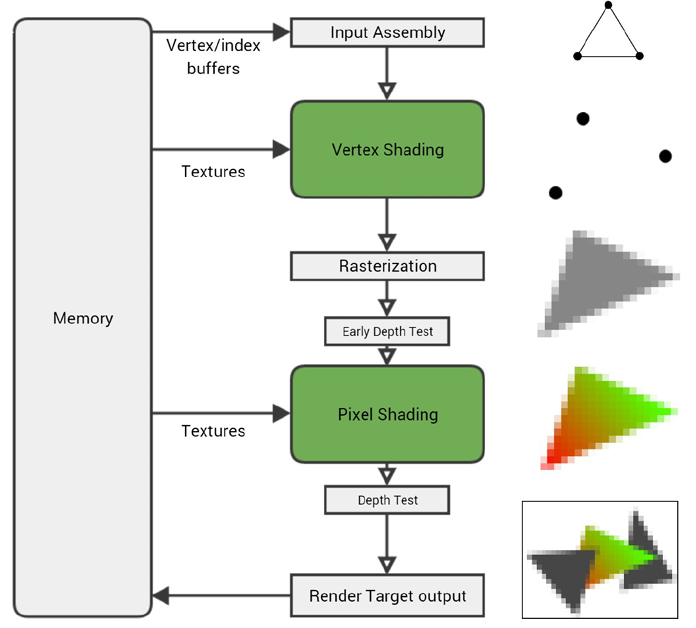
\includegraphics[width=0.5\textwidth]{figuresP/lesson_parallel_3B_pag_6.png}
\end{center}

From this oversimplified scheme you should get two important concepts: each triangle that creates an image is independent of each other (and so different processors can work simultaneously on each triangle) and the exchange of data between the memory and the GPU is constant and needs to be fast. Modern GPUs don't exactly work like this anymore, but the basic idea remains the same.

In other words, the graphics pipeline requires a huge amount of arithmetic on independent data (this includes transforming positions, generating pixel colors, and applying material properties and light situations to every pixel). The hardware requires the ability to access memory simultaneously and contiguously (considering that bandwidth is more important than latency) and needs floating-point and fixed-function logic.

We then get to the canonical definition of a GPU: it is "\textit{a single-chip processor with integrated transform, lightning, triangle setup/clipping and rendering engines that is capable of processing a minimum of 10 million polygons per second}". Apart from the hardware components specified, this definition is based on the capability of the GPU to process the triangles we were previously talking about. In fact, GPUs were invented in 1997 just for image processing ($\equiv$ "to work with triangles") and we had to wait until 2007 before NVIDIA opened the possibility to use them for generic computing (GPGPU). In 2008 a consortium of different firms decided to introduce a common multiplatform language for manycore computing called \textbf{OpenCL}.

We will not be using OpenCL during this course, but CUDA (which is used specifically for NVIDIA GPUs). These two frameworks are very similar (so it will be very easy to switch to OpenCL if you want to), but CUDA is better documented and better for learning the basics.

GPUs are a way to cheat Moore's law thanks to their SIMD/SIMT (\textit{Single Instruction Multiple Threads}, we will see what this means) parallel architecture. They offer very high computing power for vectorizable problems, with an impressive derivative that is almost a factor of 2 in each generation. Thanks to continuous development (due to higher and higher economic interest in video games and such), it is easy to have a desktop PC with teraflops\footnote{As you might already know, the number of FLOPS (\textit{Floating Point Operations per Second}) is a measurement of the computing power of a processor. Theoretically, it is defined as:
$$ \text{FLOPS} = \text{clock frequency} \cdot \text{\# cores} \cdot \text{\# operation per cycle} $$
but of course this formula doesn't take into account several things. The real estimation is made experimentally by using standard packages (LINPACK, LAPACK) and other metrics have been invented to avoid the limitations of FLOPS in measuring the computing power, such as SPECint and SPECfp.} of computing power, with thousands of cores. This leads to several applications in \textit{high-performance computing} (HPC), simulation, scientific computing etc\dots

Take a look at the specifics of some of the GPUs on the market in the tables below, and note for example the great number of cores that each one has. 

\begin{table}[H]
\centering
\resizebox{\textwidth}{!}{
\begin{tabular}{|l|l|l|l|l|l|l|}
\hline
\textbf{Tesla GPU} & \textbf{Fermi GF100} & \textbf{Fermi GF104} & \textbf{Kepler GK104} & \textbf{Kepler GK110} & \textbf{Maxwell GM200} & \textbf{Pascal GP100} \\ \hline
Compute Capability & 2.0 & 2.1 & 3.0 & 3.5 & 5.2 & 6.0 \\ \hline
Streaming Multiprocessors (SMs) & 16 & 16 & 8 & 15 & 24 & 56 \\ \hline
FP32 CUDA Cores/SM & 32 & 48 & 192 & 192 & 128 & 64 \\ \hline
FP32 CUDA Cores & 512 & 384 & 1536 & 2880 & 3072 & 3584 \\ \hline
FP64 Units & 256 & 32 & 64 & 960 & 96 & 1792 \\ \hline
Threads/Warp & 32 & 32 & 32 & 32 & 32 & 32 \\ \hline
Max Warps/Multiprocessor & 48 & 48 & 64 & 64 & 64 & 64 \\ \hline
Max Threads/Multiprocessor & 1536 & 1536 & 2048 & 2048 & 2048 & 2048 \\ \hline
Max Thread Blocks/Multiprocessor & 8 & 8 & 16 & 16 & 32 & 32 \\ \hline
32bit-Registers/Multiprocessor & 32768 & 32768 & 65536 & 65536 & 65536 & 65536 \\ \hline
Max Registers/Thread & 63 & 63 & 63 & 255 & 255 & 255 \\ \hline
Max Threads/Thread Block & 1024 & 1024 & 1024 & 1024 & 1024 & 1024 \\ \hline
Shared Memory Size Configs & 16 KB/48 KB & 16 KB/48 KB & 16 KB/32 KB/48 KB & 16 KB/32 KB/48 KB & 96 KB & 64 KB \\ \hline
Hyper-Q & No & No & No & Yes & Yes & Yes \\ \hline
Dynamic Parallelism & No & No & No & Yes & Yes & Yes \\ \hline
Unified Memory & No & No & No & No & No & Yes \\ \hline
Pre-Emption & No & No & No & No & No & Yes \\ \hline
\end{tabular}
}
\end{table}

\begin{table}[H]
\centering
\resizebox{\textwidth}{!}{%
\begin{tabular}{|l|l|l|l|l|}
\hline
\textbf{GPU} & \textbf{NVIDIA H100 (GH100)} & \textbf{NVIDIA A100 (GA100)} & \textbf{NVIDIA Tesla V100 (GV100)} & \textbf{NVIDIA Tesla P100 (GP100)} \\ \hline
Transistors & 80B & 54.2B & 21.1B & 15.3B \\ \hline
Die Size & 814 mm² & 828 mm² & 815 mm² & 610 mm² \\ \hline
Architecture & Hopper & Ampere & Volta & Pascal \\ \hline
Fabrication Node & TSMC N4 & TSMC N7 & 12nm FFN & 16nm FinFET+ \\ \hline
GPU Clusters & 132/114 & 108 & 80 & 56 \\ \hline
CUDA Cores & 16896/14592 & 6912 & 5120 & 3584 \\ \hline
L2 Cache & 50MB & 40MB & 6MB & 4MB \\ \hline
Tensor Cores & 528/456 & 432 & 320 & N/A \\ \hline
Memory Bus & 5120-bit & 5120-bit & 4096-bit & 4096-bit \\ \hline
Memory Size & 80 GB HBM3/HBM2e & 40/80GB HBM2e & 16/32 GB HBM2 & 16GB HBM2 \\ \hline
TDP & 700W/350W & 250W/300W/400W & 250W/300W/450W & 250W/300W \\ \hline
Interface & SXM5/ PCIe Gen5 & SXM4/PCIe Gen4 & SXM2/PCIe Gen3 & SXM/PCIe Gen3 \\ \hline
\end{tabular}%
}
\end{table}

\subsection{CPU vs GPU: designs and advantages}

Both CPUs and GPUs are components of about 5 cm $\times$ 5 cm, but their designs are very different and tailored for their specific applications. 

Take a look at a standard 4-core CPU in the following figure. It relies on multilevel and large caches to convert long latency memory access to short latency cache access and uses branch prediction to reduce latency in branching. It adopts Instruction level parallelism (ILP) with powerful ALUs and includes complex memory management and a large control part. In other words, a \textbf{CPU should have a latency-oriented design}. That's intuitive as it is not only used for computation, but for many other operations that require a nearly instant response for the user (e.g. if you move the mouse you want the icon on your screen to move as fast as possible). 

\begin{center}
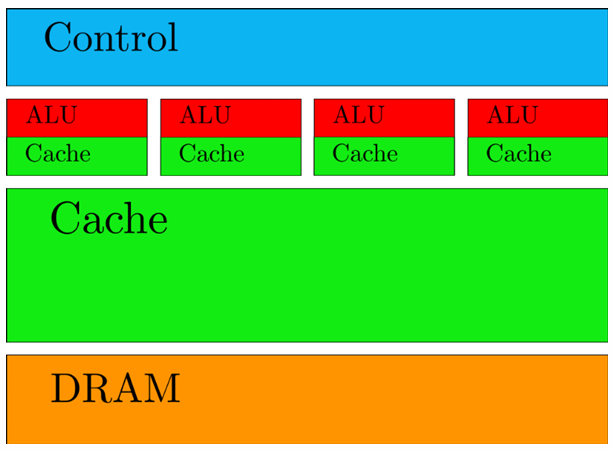
\includegraphics[width=0.3\textwidth]{figuresP/lesson_parallel_3B_pag_15.png}
\end{center}

Instead, a GPU relies on SIMT/SIMD architecture and uses SMX (Streaming Multiprocessors) to execute kernels. It exploits thread-level parallelism with massive threading to hide the latency and features limited caching, primarily to boost memory throughput, and limited control (no branch prediction, but branch predication). That means that every \textbf{GPU has a throughput-oriented design} to maximize its computing capabilities. 

\begin{center}
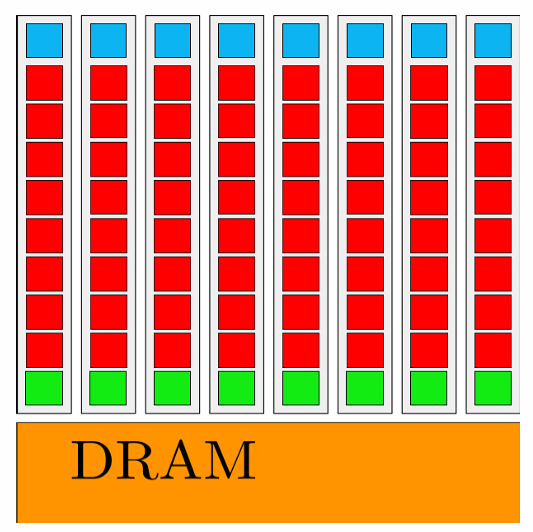
\includegraphics[width=0.3\textwidth]{figuresP/lesson_parallel_3B_pag_16.png}
\end{center}

Below you will find a schematic comparison of the characteristics of a generic CPU and GPU and a table with the specifics of a real CPU and a GPU of the same generation.

\begin{center}
    % Prima colonna: CPU
    \begin{minipage}[t]{0.45\textwidth}
        \centering
        \underline{CPU}\par
        \vspace{0.5em}
        \normalsize
        \begin{itemize}
            \item[+] Large main memory
            \item[+] Fast clock rate
            \item[+] Large caches
            \item[+] Branch prediction
            \item[+] Powerful ALU
            \item[-] Relatively low memory bandwidth
            \item[-] Cache misses costly
            \item[-] Low performance per watt
        \end{itemize}
    \end{minipage}\hfill
    % Seconda colonna: GPU
    \begin{minipage}[t]{0.45\textwidth}
        \centering
        \underline{GPU}\par
        \vspace{0.5em}
        \normalsize
        \begin{itemize}
            \item[+] High bandwidth main memory
            \item[+] Latency tolerant (parallelism)
            \item[+] More compute resources
            \item[+] High performance per watt
            \item[-] Limited memory capacity
            \item[-] Low per-thread performance
            \item[-] Extension card
        \end{itemize}
    \end{minipage}
\end{center}

\begin{center}
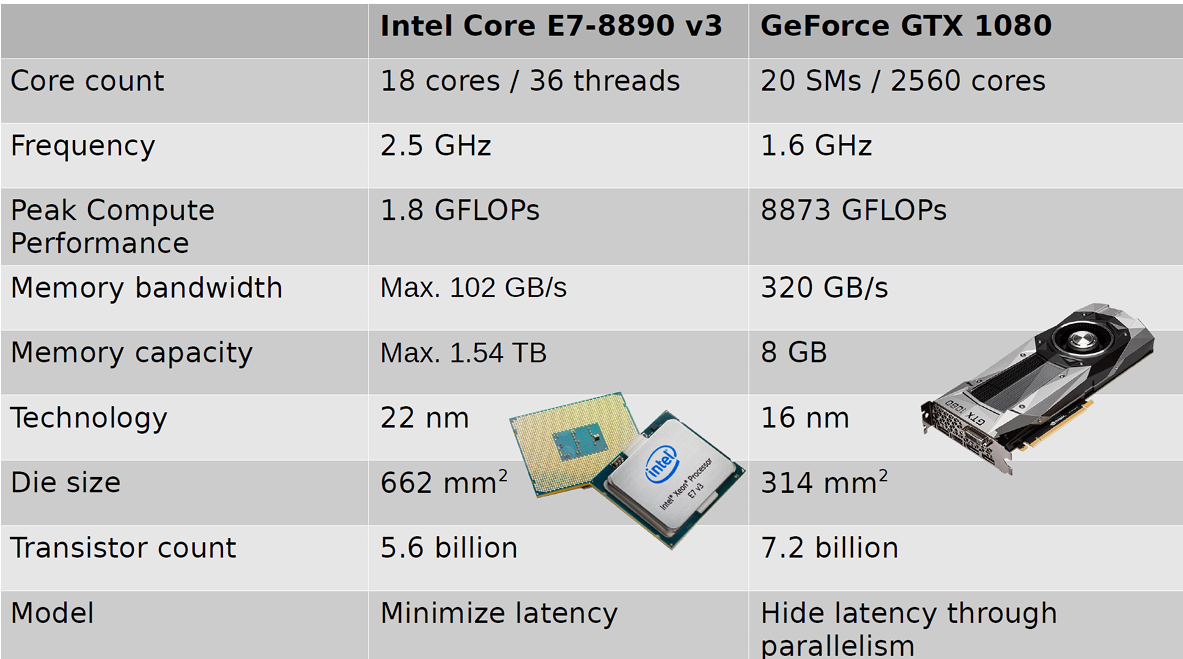
\includegraphics[width=0.6\textwidth]{figuresP/lesson_parallel_3B_pag_19.png}
\end{center}

The winning application uses both CPUs and GPUs, as suggested by Amdahl's law: CPUs are used for sequential parts (they can be 10$\times$ faster than GPUs for sequential code), while GPUs are used for parallel ones, where throughput is fundamental (they can be 100$\times$ faster than CPUs for parallel code). As we will see, what causes the most latency is the exchange of data between these components, and we will learn how to reduce it as much as possible. 

\subsection{Single Instruction Multiple Threads (SIMT) architecture}

\begin{center}
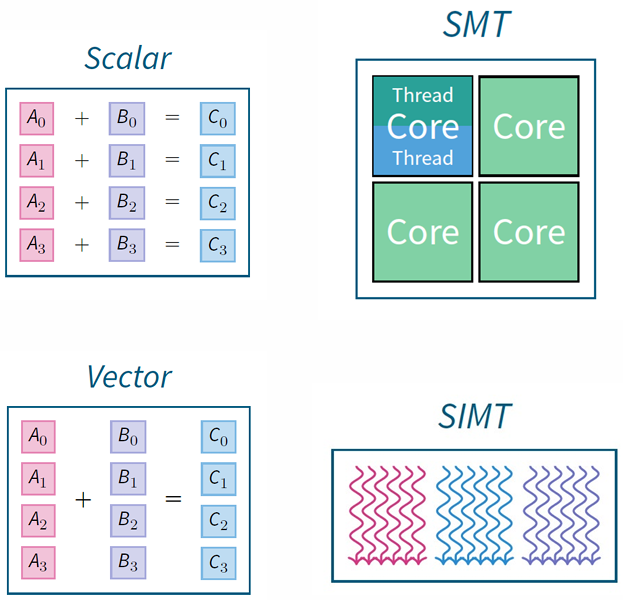
\includegraphics[width=0.35\textwidth]{figuresP/lesson_parallel_3B_pag_21.png}
\end{center}

A SIMD architecture is not the right choice for a GPU. In a SIMD multicore processor, we have to execute the same instruction ($\equiv$ the same line of code, the same thread) on different pieces of data for each core, so they cannot work completely independently. We will see in the next lesson that a GPU is composed of many multiprocessors that actually work as a SIMD architecture, similarly to a multicore CPU. However, each multiprocessor can execute different parts of the same program or completely different programs. That's what we call a \textbf{Single Instruction Multiple Threads (SIMT)} architecture.
\section{Introduction to GPU computing (2)}

\begin{figure}[htbp]
    \begin{minipage}[c]{0.55\textwidth}
        Now that we know what a GPU is, let's introduce some more accurate terminology. First of all, the GPU will be connected to your computer through the so called \textbf{Bus PCI Express} on your mother board. We are going to call \textbf{host} the computer to which the GPU is connected and \textbf{device} the GPU itself. The host contains the CPU and the RAM: the serial part of our programs is going to run on that. The part of our code that runs on the GPU is called the \textbf{kernel} and its execution consists in 3 main steps:
        \begin{enumerate}
            \item copy the data from the host (hard disk or RAM) to the device;
            \item copy the kernel and execute;
            \item copy back results.
        \end{enumerate}
        With that said, what is \textbf{CUDA}?  It is a set of C/C++ extensions to enable GPU computing on NVIDIA GPUs. In other words, it is a framework that enables you to go through all those 3 phases of execution. Dedicated APIs allow to control almost all the functions of the graphics processor.
    \end{minipage}\hfill 
    \begin{minipage}[c]{0.42\textwidth}
        \centering
        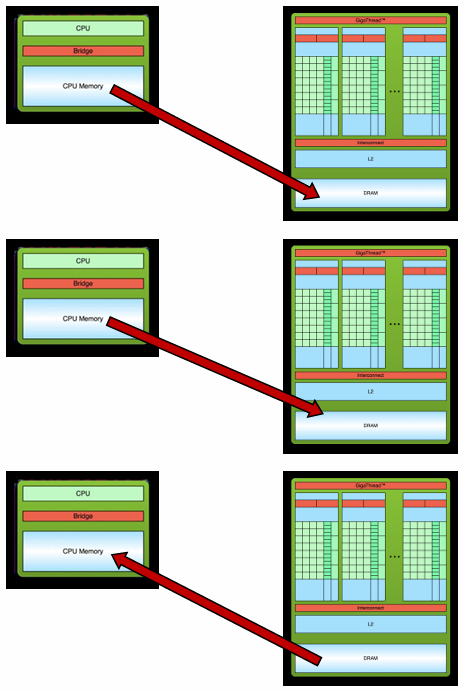
\includegraphics[width=\textwidth]{figuresP/lesson_parallel_4_pag_3.png}
    \end{minipage}
\end{figure}

\subsection{Blocks $\rightarrow$ multiprocessors , threads $\rightarrow$ cores}
Take a look at the schematic representation of a GPU below.

\begin{center}
    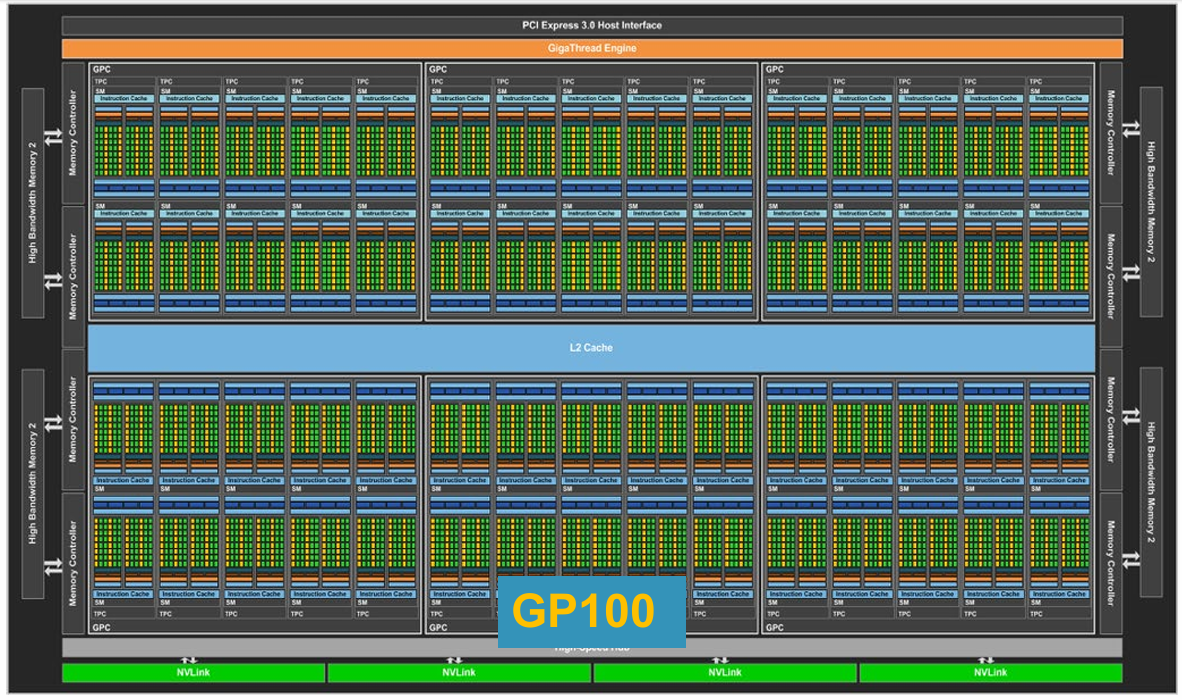
\includegraphics[width=\textwidth]{figuresP/lesson_parallel_4_pag_5.png}
\end{center}

As said before, a GPU is composed of simpler structures called \textbf{multiprocessors} that contain a grid of cores. Each multiprocessor has a SIMD architecture, so each core must execute the same instruction, but different multiprocessors can execute different parts of the program (SIMT). Take a look at the physical structure of a multiprocessor in the figure below.

\begin{center}
    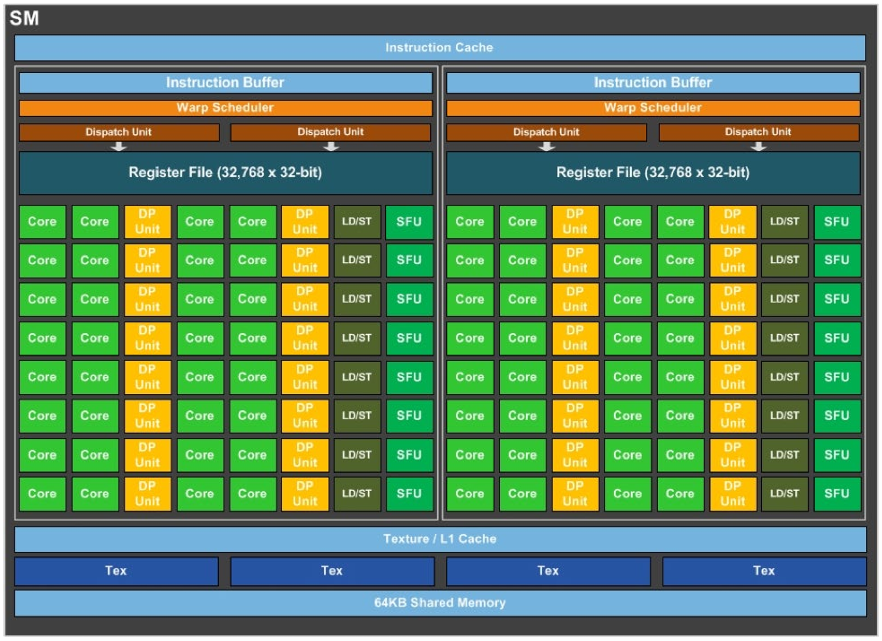
\includegraphics[width=0.8\textwidth]{figuresP/lesson_parallel_4_pag_6.png}
\end{center}

There is an important analogy between how a GPU is physically built and how a program that is supposed to run on it can be organized. A group of threads that can communicate and synchronize (i.e. execute the same instruction at the same time) is called a \textbf{block} (and a group of block is called a \textit{grid}). Threads in different blocks do not interact. 

To understand this concept let's imagine a simple situation. Let's say that we have a GPU with 1000 cores grouped in 10 multiprocessors. Intuitively, one could say that on this GPU you can run 10 blocks with 100 threads each, but that would be wrong. \\ Inside each multiprocessor there is a component called \textbf{instruction buffer} or "\textbf{small scheduler}". If each block contains 300 threads, the scheduler will send the first 100 threads to the cores to be executed and then the remaining 200 to the cores that concluded their execution. \\ Similarly, a GPU must have a "\textbf{big scheduler}" that distributes blocks to the multiprocessors in the same way. The terms "small" and "big" come from the fact that the GPU scheduler can manage thousands of billions of blocks, while the multiprocessor one is usually limited to 2048 threads at a time. \\ That means that the analogy "threads $\rightarrow$ cores" and "blocks $\rightarrow$ multiprocessors" is of course not perfect, since a GPU can manage a much larger number of blocks than the number of multiprocessors it has.  

\subsection{Memory hierarchy}

As we can observe from the architectural schematics above, understanding the memory hierarchy is fundamental in GPU programming. Unlike modern CPUs, where caching is mostly transparent, on a GPU a significant portion of memory management and data locality optimization is explicitly left to the programmer. Memory is structured into a hierarchy based on physical location, speed, and scope:

\begin{itemize}
    \item \textbf{Global Memory}: This is the main memory of the GPU (labeled as \textit{High Bandwidth Memory} on in the GPU figure above). It is located "off-chip" on the GPU board, meaning it has the highest latency and is relatively slow. However, it is vast, lasts for the entire lifetime of the application, and is universally accessible: both the host and all threads across all grids on the device can read and write to it. As seen in the first figure, accesses to global memory are typically buffered through a large, shared \textbf{L2 Cache} located in the centre of the GPU.
    
    \item \textbf{Shared Memory}: Looking at the multiprocessor diagram, you can clearly spot a dedicated block labeled \textit{64KB Shared Memory} at the bottom. Because it resides directly "on-chip" within the multiprocessor, it is extremely fast. This memory is allocated \textit{per-block}: it is readable and writable by all threads within the same block, allowing them to synchronize and share data efficiently. Its lifetime is tied strictly to the execution of that specific block.
    
    \item \textbf{Registers (Private Memory)}: The same figure also prominently features massive \textit{Register Files} (e.g., $32,768 \times 32$-bit) sitting right above the processing cores. Registers represent the fastest type of memory available. They are allocated on a \textit{per-thread} basis. The data stored here is strictly private, meaning it is only readable and writable by the individual thread that owns it, and its scope lasts only for the lifetime of that single thread.
\end{itemize}

The problem is that memory transfer is comparably slow. The solution is to do something else in the meantime, like some more computation. You can overlap tasks by having copy and compute engines run separately (\textit{asynchronicity}). The CPU can do other work while the GPU computes, handling synchronization when needed. This will work only on modern GPUs and we will not dive deeper into this method. 

\begin{center}
    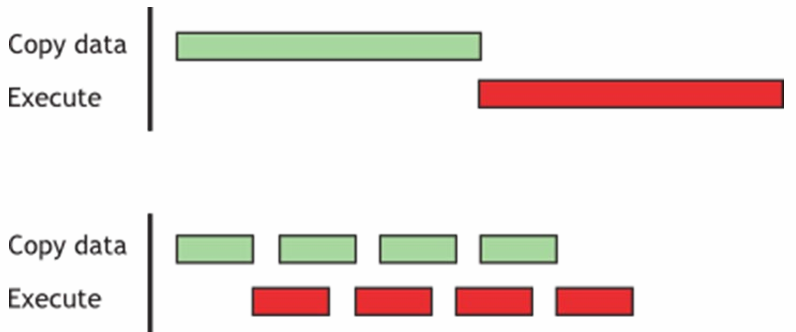
\includegraphics[width=0.4\textwidth]{figuresP/lesson_parallel_4_pag_8.png}
\end{center}

\subsection{How to program a GPU?}

There are entire courses and books dedicated to GPU programming. Here you are going to get the general idea and learn the basics that are imperative if you want to delve deeper into the topic in the future.

CUDA is the "best" way to program NVIDIA GPUs at a low level. If your code is almost all CPU (as in many applications to data analysis in physics) or if you need to accelerate dedicated functions, you could consider using \textit{directives} (OpenMP, OpenACC) or \textit{libraries} (Thrust, ArrayFire, cuBLAS, cuFFT, etc.). These tools lets you use the GPUs at a high level, sometimes without even knowing it. OpenCL is a framework equivalent to CUDA used to program multiplatforms (GPU, CPU, DSP, FPGA). C/C++ and Fortran are the "official" languages for CUDA, while Python and other languages are supported through wrapping and libraries (like Numba, PyCUDA, Theano).

Take a rapid look at the following examples in C (you don't have to remember them).

\subsubsection{- Libraries: \texttt{Thrust}}

\texttt{Thrust} is a template library for data parallel primitives (such as \texttt{scan()}, \texttt{sort()}, \texttt{reduce()}, etc...). It comes for free when you install CUDA.

\begin{Verbatim}[label=\makebox{\url{https://github.com/lucabaldini/cmepda/tree/master/slides/latex/snippets/thrust_saxpy.cu}},commandchars=\\\{\}]
\PY{c+cp}{\#}\PY{c+cp}{include}\PY{+w}{ }\PY{c+cpf}{\PYZlt{}thrust/host\_vector.h\PYZgt{}}
\PY{c+cp}{\#}\PY{c+cp}{include}\PY{+w}{ }\PY{c+cpf}{\PYZlt{}thrust/device\_vector.h\PYZgt{}}
\PY{c+cp}{\#}\PY{c+cp}{include}\PY{+w}{ }\PY{c+cpf}{\PYZlt{}thrust/transform.h\PYZgt{}}

\PY{k+kt}{int}\PY{+w}{ }\PY{n+nf}{main}\PY{p}{(}\PY{p}{)}\PY{+w}{ }\PY{p}{\PYZob{}}
\PY{+w}{    }\PY{k+kt}{float}\PY{+w}{ }\PY{n}{a}\PY{+w}{ }\PY{o}{=}\PY{+w}{ }\PY{l+m+mf}{42.0f}\PY{p}{;}
\PY{+w}{    }\PY{k+kt}{int}\PY{+w}{ }\PY{n}{n}\PY{+w}{ }\PY{o}{=}\PY{+w}{ }\PY{l+m+mi}{10}\PY{p}{;}

\PY{+w}{    }\PY{c+c1}{// Create vectors residing in CPU memory}
\PY{+w}{    }\PY{n}{thrust}\PY{o}{:}\PY{o}{:}\PY{n}{host\_vector}\PY{o}{\PYZlt{}}\PY{k+kt}{float}\PY{o}{\PYZgt{}}\PY{+w}{ }\PY{n}{x}\PY{p}{(}\PY{n}{n}\PY{p}{)}\PY{p}{,}\PY{+w}{ }\PY{n}{y}\PY{p}{(}\PY{n}{n}\PY{p}{)}\PY{p}{;}

\PY{+w}{    }\PY{c+c1}{// Initialize arrays with dummy data}
\PY{+w}{    }\PY{k}{for}\PY{p}{(}\PY{k+kt}{int}\PY{+w}{ }\PY{n}{i}\PY{+w}{ }\PY{o}{=}\PY{+w}{ }\PY{l+m+mi}{0}\PY{p}{;}\PY{+w}{ }\PY{n}{i}\PY{+w}{ }\PY{o}{\PYZlt{}}\PY{+w}{ }\PY{n}{n}\PY{p}{;}\PY{+w}{ }\PY{n}{i}\PY{o}{+}\PY{o}{+}\PY{p}{)}\PY{+w}{ }\PY{p}{\PYZob{}}
\PY{+w}{        }\PY{n}{x}\PY{p}{[}\PY{n}{i}\PY{p}{]}\PY{+w}{ }\PY{o}{=}\PY{+w}{ }\PY{l+m+mf}{1.0f}\PY{p}{;}
\PY{+w}{        }\PY{n}{y}\PY{p}{[}\PY{n}{i}\PY{p}{]}\PY{+w}{ }\PY{o}{=}\PY{+w}{ }\PY{l+m+mf}{2.0f}\PY{p}{;}
\PY{+w}{    }\PY{p}{\PYZcb{}}

\PY{+w}{    }\PY{c+c1}{// Create GPU vectors and implicitly copy data from CPU to GPU}
\PY{+w}{    }\PY{n}{thrust}\PY{o}{:}\PY{o}{:}\PY{n}{device\_vector}\PY{o}{\PYZlt{}}\PY{k+kt}{float}\PY{o}{\PYZgt{}}\PY{+w}{ }\PY{n}{d\_x}\PY{+w}{ }\PY{o}{=}\PY{+w}{ }\PY{n}{x}\PY{p}{,}\PY{+w}{ }\PY{n}{d\_y}\PY{+w}{ }\PY{o}{=}\PY{+w}{ }\PY{n}{y}\PY{p}{;}

\PY{+w}{    }\PY{k}{using}\PY{+w}{ }\PY{k}{namespace}\PY{+w}{ }\PY{n+nn}{thrust}\PY{o}{:}\PY{o}{:}\PY{n+nn}{placeholders}\PY{p}{;}

\PY{+w}{    }\PY{c+c1}{// Apply parallel transformation on GPU.}
\PY{+w}{    }\PY{c+c1}{// \_1 and \_2 are placeholders for the elements of d\_x and d\_y.}
\PY{+w}{    }\PY{n}{thrust}\PY{o}{:}\PY{o}{:}\PY{n}{transform}\PY{p}{(}\PY{n}{d\_x}\PY{p}{.}\PY{n}{begin}\PY{p}{(}\PY{p}{)}\PY{p}{,}\PY{+w}{ }\PY{n}{d\_x}\PY{p}{.}\PY{n}{end}\PY{p}{(}\PY{p}{)}\PY{p}{,}\PY{+w}{ }\PY{n}{d\_y}\PY{p}{.}\PY{n}{begin}\PY{p}{(}\PY{p}{)}\PY{p}{,}\PY{+w}{ }\PY{n}{d\_y}\PY{p}{.}\PY{n}{begin}\PY{p}{(}\PY{p}{)}\PY{p}{,}\PY{+w}{ }\PY{n}{a}\PY{+w}{ }\PY{o}{*}\PY{+w}{ }\PY{n}{\_1}\PY{+w}{ }\PY{o}{+}\PY{+w}{ }\PY{n}{\_2}\PY{p}{)}\PY{p}{;}

\PY{+w}{    }\PY{c+c1}{// Implicitly copy the result back to CPU memory}
\PY{+w}{    }\PY{n}{y}\PY{+w}{ }\PY{o}{=}\PY{+w}{ }\PY{n}{d\_y}\PY{p}{;}

\PY{+w}{    }\PY{k}{return}\PY{+w}{ }\PY{l+m+mi}{0}\PY{p}{;}
\PY{p}{\PYZcb{}}
\end{Verbatim}

\subsubsection{- Libraries: \texttt{cuBLAS}}

\texttt{cuBLAS} provides GPU-parallel linear algebra routines (152 routines) supporting single, double, and complex data types. It also offers the possibility to use multiple GPUs. A classic example is the \texttt{Saxpy} routine: given two vectors $x[10]$ and $y[10]$, it computes $y[i] = a \cdot x[i] + y[i]$.

\begin{Verbatim}[label=\makebox{\url{https://github.com/lucabaldini/cmepda/tree/master/slides/latex/snippets/cublas_saxpy.cpp}},commandchars=\\\{\}]
\PY{c+cp}{\#}\PY{c+cp}{include}\PY{+w}{ }\PY{c+cpf}{\PYZlt{}iostream\PYZgt{}}
\PY{c+cp}{\#}\PY{c+cp}{include}\PY{+w}{ }\PY{c+cpf}{\PYZlt{}cublas\_v2.h\PYZgt{}}

\PY{k+kt}{int}\PY{+w}{ }\PY{n+nf}{main}\PY{p}{(}\PY{p}{)}\PY{+w}{ }\PY{p}{\PYZob{}}
\PY{+w}{    }\PY{k+kt}{float}\PY{+w}{ }\PY{n}{a}\PY{+w}{ }\PY{o}{=}\PY{+w}{ }\PY{l+m+mf}{42.0f}\PY{p}{;}
\PY{+w}{    }\PY{k}{const}\PY{+w}{ }\PY{k+kt}{int}\PY{+w}{ }\PY{n}{n}\PY{+w}{ }\PY{o}{=}\PY{+w}{ }\PY{l+m+mi}{10}\PY{p}{;}
\PY{+w}{    }\PY{k+kt}{float}\PY{+w}{ }\PY{n}{x}\PY{p}{[}\PY{n}{n}\PY{p}{]}\PY{p}{,}\PY{+w}{ }\PY{n}{y}\PY{p}{[}\PY{n}{n}\PY{p}{]}\PY{p}{;}

\PY{+w}{    }\PY{c+c1}{// Initialize arrays with dummy data}
\PY{+w}{    }\PY{k}{for}\PY{+w}{ }\PY{p}{(}\PY{k+kt}{int}\PY{+w}{ }\PY{n}{i}\PY{+w}{ }\PY{o}{=}\PY{+w}{ }\PY{l+m+mi}{0}\PY{p}{;}\PY{+w}{ }\PY{n}{i}\PY{+w}{ }\PY{o}{\PYZlt{}}\PY{+w}{ }\PY{n}{n}\PY{p}{;}\PY{+w}{ }\PY{n}{i}\PY{o}{+}\PY{o}{+}\PY{p}{)}\PY{+w}{ }\PY{p}{\PYZob{}}
\PY{+w}{        }\PY{n}{x}\PY{p}{[}\PY{n}{i}\PY{p}{]}\PY{+w}{ }\PY{o}{=}\PY{+w}{ }\PY{l+m+mf}{1.0f}\PY{p}{;}
\PY{+w}{        }\PY{n}{y}\PY{p}{[}\PY{n}{i}\PY{p}{]}\PY{+w}{ }\PY{o}{=}\PY{+w}{ }\PY{l+m+mf}{2.0f}\PY{p}{;}
\PY{+w}{    }\PY{p}{\PYZcb{}}

\PY{+w}{    }\PY{c+c1}{// Initialize the cuBLAS library context}
\PY{+w}{    }\PY{n}{cublasHandle\_t}\PY{+w}{ }\PY{n}{handle}\PY{p}{;}
\PY{+w}{    }\PY{n}{cublasCreate}\PY{p}{(}\PY{o}{\PYZam{}}\PY{n}{handle}\PY{p}{)}\PY{p}{;}

\PY{+w}{    }\PY{k+kt}{float}\PY{+w}{ }\PY{o}{*}\PY{+w}{ }\PY{n}{d\_x}\PY{p}{,}\PY{+w}{ }\PY{o}{*}\PY{+w}{ }\PY{n}{d\_y}\PY{p}{;}
\PY{+w}{    }\PY{c+c1}{// Allocate memory exclusively on the GPU (Device memory)}
\PY{+w}{    }\PY{n}{cudaMalloc}\PY{p}{(}\PY{p}{(}\PY{k+kt}{void}\PY{+w}{ }\PY{o}{*}\PY{o}{*}\PY{p}{)}\PY{o}{\PYZam{}}\PY{n}{d\_x}\PY{p}{,}\PY{+w}{ }\PY{n}{n}\PY{+w}{ }\PY{o}{*}\PY{+w}{ }\PY{k}{sizeof}\PY{p}{(}\PY{n}{x}\PY{p}{[}\PY{l+m+mi}{0}\PY{p}{]}\PY{p}{)}\PY{p}{)}\PY{p}{;}
\PY{+w}{    }\PY{n}{cudaMalloc}\PY{p}{(}\PY{p}{(}\PY{k+kt}{void}\PY{+w}{ }\PY{o}{*}\PY{o}{*}\PY{p}{)}\PY{o}{\PYZam{}}\PY{n}{d\_y}\PY{p}{,}\PY{+w}{ }\PY{n}{n}\PY{+w}{ }\PY{o}{*}\PY{+w}{ }\PY{k}{sizeof}\PY{p}{(}\PY{n}{y}\PY{p}{[}\PY{l+m+mi}{0}\PY{p}{]}\PY{p}{)}\PY{p}{)}\PY{p}{;}

\PY{+w}{    }\PY{c+c1}{// Copy data from CPU (Host) to GPU (Device)}
\PY{+w}{    }\PY{n}{cublasSetVector}\PY{p}{(}\PY{n}{n}\PY{p}{,}\PY{+w}{ }\PY{k}{sizeof}\PY{p}{(}\PY{n}{x}\PY{p}{[}\PY{l+m+mi}{0}\PY{p}{]}\PY{p}{)}\PY{p}{,}\PY{+w}{ }\PY{n}{x}\PY{p}{,}\PY{+w}{ }\PY{l+m+mi}{1}\PY{p}{,}\PY{+w}{ }\PY{n}{d\_x}\PY{p}{,}\PY{+w}{ }\PY{l+m+mi}{1}\PY{p}{)}\PY{p}{;}
\PY{+w}{    }\PY{n}{cublasSetVector}\PY{p}{(}\PY{n}{n}\PY{p}{,}\PY{+w}{ }\PY{k}{sizeof}\PY{p}{(}\PY{n}{y}\PY{p}{[}\PY{l+m+mi}{0}\PY{p}{]}\PY{p}{)}\PY{p}{,}\PY{+w}{ }\PY{n}{y}\PY{p}{,}\PY{+w}{ }\PY{l+m+mi}{1}\PY{p}{,}\PY{+w}{ }\PY{n}{d\_y}\PY{p}{,}\PY{+w}{ }\PY{l+m+mi}{1}\PY{p}{)}\PY{p}{;}

\PY{+w}{    }\PY{c+c1}{// Execute the optimized SAXPY library function on GPU}
\PY{+w}{    }\PY{n}{cublasSaxpy}\PY{p}{(}\PY{n}{handle}\PY{p}{,}\PY{+w}{ }\PY{n}{n}\PY{p}{,}\PY{+w}{ }\PY{o}{\PYZam{}}\PY{n}{a}\PY{p}{,}\PY{+w}{ }\PY{n}{d\_x}\PY{p}{,}\PY{+w}{ }\PY{l+m+mi}{1}\PY{p}{,}\PY{+w}{ }\PY{n}{d\_y}\PY{p}{,}\PY{+w}{ }\PY{l+m+mi}{1}\PY{p}{)}\PY{p}{;}

\PY{+w}{    }\PY{c+c1}{// Copy the result back from GPU to CPU}
\PY{+w}{    }\PY{n}{cublasGetVector}\PY{p}{(}\PY{n}{n}\PY{p}{,}\PY{+w}{ }\PY{k}{sizeof}\PY{p}{(}\PY{n}{y}\PY{p}{[}\PY{l+m+mi}{0}\PY{p}{]}\PY{p}{)}\PY{p}{,}\PY{+w}{ }\PY{n}{d\_y}\PY{p}{,}\PY{+w}{ }\PY{l+m+mi}{1}\PY{p}{,}\PY{+w}{ }\PY{n}{y}\PY{p}{,}\PY{+w}{ }\PY{l+m+mi}{1}\PY{p}{)}\PY{p}{;}

\PY{+w}{    }\PY{c+c1}{// Clean up GPU memory and destroy cuBLAS context}
\PY{+w}{    }\PY{n}{cudaFree}\PY{p}{(}\PY{n}{d\_x}\PY{p}{)}\PY{p}{;}
\PY{+w}{    }\PY{n}{cudaFree}\PY{p}{(}\PY{n}{d\_y}\PY{p}{)}\PY{p}{;}
\PY{+w}{    }\PY{n}{cublasDestroy}\PY{p}{(}\PY{n}{handle}\PY{p}{)}\PY{p}{;}

\PY{+w}{    }\PY{k}{return}\PY{+w}{ }\PY{l+m+mi}{0}\PY{p}{;}
\PY{p}{\PYZcb{}}
\end{Verbatim}

\subsubsection{- Directives: OpenMP, OpenACC}

Directives are the best transparent way to use the GPU. You must only \textit{annotate} the part of the code you want to parallelize (the example below uses the annotation \texttt{\# pragma acc kernels} to parallelize the \texttt{for} loop). Directives are portable and easy to program, but not all the raw GPU power is available when using them. The code also becomes harder to debug, and it is easy to program wrong. \texttt{OpenACC} is more focused on GPU, while \texttt{OpenMP} is for multi-computers (but still usable with GPU).

\begin{Verbatim}[label=\makebox{\url{https://github.com/lucabaldini/cmepda/tree/master/slides/latex/snippets/openacc_saxpy.cpp}},commandchars=\\\{\}]
\PY{c+cp}{\#}\PY{c+cp}{include}\PY{+w}{ }\PY{c+cpf}{\PYZlt{}iostream\PYZgt{}}

\PY{k+kt}{void}\PY{+w}{ }\PY{n+nf}{saxpy\_acc}\PY{p}{(}\PY{k+kt}{int}\PY{+w}{ }\PY{n}{n}\PY{p}{,}\PY{+w}{ }\PY{k+kt}{float}\PY{+w}{ }\PY{n}{a}\PY{p}{,}\PY{+w}{ }\PY{k+kt}{float}\PY{+w}{ }\PY{o}{*}\PY{+w}{ }\PY{n}{x}\PY{p}{,}\PY{+w}{ }\PY{k+kt}{float}\PY{+w}{ }\PY{o}{*}\PY{+w}{ }\PY{n}{y}\PY{p}{)}\PY{+w}{ }\PY{p}{\PYZob{}}
\PY{+w}{    }\PY{c+c1}{// Instruct compiler to parallelize this loop on GPU}
\PY{+w}{    }\PY{c+c1}{// and explicitly handle data copy from/to GPU memory}
\PY{+w}{    }\PY{c+cp}{\#}\PY{c+cp}{pragma acc kernels copyin(x[0:n]) copy(y[0:n])}
\PY{+w}{    }\PY{k}{for}\PY{+w}{ }\PY{p}{(}\PY{k+kt}{int}\PY{+w}{ }\PY{n}{i}\PY{+w}{ }\PY{o}{=}\PY{+w}{ }\PY{l+m+mi}{0}\PY{p}{;}\PY{+w}{ }\PY{n}{i}\PY{+w}{ }\PY{o}{\PYZlt{}}\PY{+w}{ }\PY{n}{n}\PY{p}{;}\PY{+w}{ }\PY{n}{i}\PY{o}{+}\PY{o}{+}\PY{p}{)}\PY{+w}{ }\PY{p}{\PYZob{}}
\PY{+w}{        }\PY{c+c1}{// Parallelized SAXPY operation}
\PY{+w}{        }\PY{n}{y}\PY{p}{[}\PY{n}{i}\PY{p}{]}\PY{+w}{ }\PY{o}{=}\PY{+w}{ }\PY{n}{a}\PY{+w}{ }\PY{o}{*}\PY{+w}{ }\PY{n}{x}\PY{p}{[}\PY{n}{i}\PY{p}{]}\PY{+w}{ }\PY{o}{+}\PY{+w}{ }\PY{n}{y}\PY{p}{[}\PY{n}{i}\PY{p}{]}\PY{p}{;}
\PY{+w}{    }\PY{p}{\PYZcb{}}
\PY{p}{\PYZcb{}}

\PY{k+kt}{int}\PY{+w}{ }\PY{n+nf}{main}\PY{p}{(}\PY{p}{)}\PY{+w}{ }\PY{p}{\PYZob{}}
\PY{+w}{    }\PY{k+kt}{float}\PY{+w}{ }\PY{n}{a}\PY{+w}{ }\PY{o}{=}\PY{+w}{ }\PY{l+m+mf}{42.0f}\PY{p}{;}
\PY{+w}{    }\PY{k}{const}\PY{+w}{ }\PY{k+kt}{int}\PY{+w}{ }\PY{n}{n}\PY{+w}{ }\PY{o}{=}\PY{+w}{ }\PY{l+m+mi}{10}\PY{p}{;}
\PY{+w}{    }\PY{k+kt}{float}\PY{+w}{ }\PY{n}{x}\PY{p}{[}\PY{n}{n}\PY{p}{]}\PY{p}{,}\PY{+w}{ }\PY{n}{y}\PY{p}{[}\PY{n}{n}\PY{p}{]}\PY{p}{;}
\PY{+w}{    }\PY{c+c1}{// Initialize arrays with dummy data}
\PY{+w}{    }\PY{k}{for}\PY{p}{(}\PY{k+kt}{int}\PY{+w}{ }\PY{n}{i}\PY{+w}{ }\PY{o}{=}\PY{+w}{ }\PY{l+m+mi}{0}\PY{p}{;}\PY{+w}{ }\PY{n}{i}\PY{+w}{ }\PY{o}{\PYZlt{}}\PY{+w}{ }\PY{n}{n}\PY{p}{;}\PY{+w}{ }\PY{n}{i}\PY{o}{+}\PY{o}{+}\PY{p}{)}\PY{+w}{ }\PY{p}{\PYZob{}}
\PY{+w}{        }\PY{n}{x}\PY{p}{[}\PY{n}{i}\PY{p}{]}\PY{+w}{ }\PY{o}{=}\PY{+w}{ }\PY{l+m+mf}{1.0f}\PY{p}{;}
\PY{+w}{        }\PY{n}{y}\PY{p}{[}\PY{n}{i}\PY{p}{]}\PY{+w}{ }\PY{o}{=}\PY{+w}{ }\PY{l+m+mf}{2.0f}\PY{p}{;}
\PY{+w}{    }\PY{p}{\PYZcb{}}
\PY{+w}{    }\PY{c+c1}{// Launch the OpenACC parallelized function}
\PY{+w}{    }\PY{n}{saxpy\_acc}\PY{p}{(}\PY{n}{n}\PY{p}{,}\PY{+w}{ }\PY{n}{a}\PY{p}{,}\PY{+w}{ }\PY{n}{x}\PY{p}{,}\PY{+w}{ }\PY{n}{y}\PY{p}{)}\PY{p}{;}
\PY{+w}{    }\PY{k}{return}\PY{+w}{ }\PY{l+m+mi}{0}\PY{p}{;}
\PY{p}{\PYZcb{}}
\end{Verbatim}

\begin{comment}
\subsection{Direct Programming: CUDA vs OpenCL}

These are two alternative ways to directly program the GPU.
\begin{itemize}
    \item \textbf{CUDA (2007)}: NVIDIA GPU's Platform. It includes drivers, programming language (CUDA C/C++), API, compiler (nvcc), debuggers, and profilers. It works only on NVIDIA GPUs.
    \item \textbf{OpenCL (2009)}: Open Computing Language by the Khronos Group consortium (Apple, IBM, AMD, NVIDIA, etc.). It includes programming language (OpenCL C/C++), API, and compiler. It targets CPUs, GPUs, FPGAs, and other many-core machines, and it is fully open source.
\end{itemize}
\end{comment}

\subsubsection{- Direct programming with CUDA: \texttt{Saxpy} in CUDA}

The examples above were all written in the C++ language. Take a look at how we can rewrite the \texttt{cuBLAS} in full CUDA language (note that the \texttt{for} cycle is gone). As you can see, first the data must be copied on the device from the host, then the kernel is launched. The architecture of threads and blocks is decided at run time with the instruction \texttt{saxpy\_cuda <<<2, 5>>>(n, a, x, y)}.

\begin{Verbatim}[label=\makebox{\url{https://github.com/lucabaldini/cmepda/tree/master/slides/latex/snippets/cuda_saxpy.cu}},commandchars=\\\{\}]
\PY{c+cp}{\#}\PY{c+cp}{include}\PY{+w}{ }\PY{c+cpf}{\PYZlt{}iostream\PYZgt{}}

\PY{c+c1}{// Kernel function executed by the GPU}
\PY{k+kr}{\_\_global\_\_}\PY{+w}{ }\PY{k+kt}{void}\PY{+w}{ }\PY{n}{saxpy\_cuda}\PY{p}{(}\PY{k+kt}{int}\PY{+w}{ }\PY{n}{n}\PY{p}{,}\PY{+w}{ }\PY{k+kt}{float}\PY{+w}{ }\PY{n}{a}\PY{p}{,}\PY{+w}{ }\PY{k+kt}{float}\PY{+w}{ }\PY{o}{*}\PY{n}{x}\PY{p}{,}\PY{+w}{ }\PY{k+kt}{float}\PY{+w}{ }\PY{o}{*}\PY{n}{y}\PY{p}{)}\PY{+w}{ }\PY{p}{\PYZob{}}
\PY{+w}{    }\PY{c+c1}{// Calculate the unique global thread ID}
\PY{+w}{    }\PY{k+kt}{int}\PY{+w}{ }\PY{n}{i}\PY{+w}{ }\PY{o}{=}\PY{+w}{ }\PY{n+nb}{blockIdx}\PY{p}{.}\PY{n}{x}\PY{+w}{ }\PY{o}{*}\PY{+w}{ }\PY{n+nb}{blockDim}\PY{p}{.}\PY{n}{x}\PY{+w}{ }\PY{o}{+}\PY{+w}{ }\PY{n+nb}{threadIdx}\PY{p}{.}\PY{n}{x}\PY{p}{;}

\PY{+w}{    }\PY{c+c1}{// Ensure thread doesn\PYZsq{}t access out\_of\_bounds memory}
\PY{+w}{    }\PY{k}{if}\PY{+w}{ }\PY{p}{(}\PY{n}{i}\PY{+w}{ }\PY{o}{\PYZlt{}}\PY{+w}{ }\PY{n}{n}\PY{p}{)}\PY{+w}{ }\PY{p}{\PYZob{}}
\PY{+w}{        }\PY{c+c1}{// Perform the SAXPY math operation}
\PY{+w}{        }\PY{n}{y}\PY{p}{[}\PY{n}{i}\PY{p}{]}\PY{+w}{ }\PY{o}{=}\PY{+w}{ }\PY{n}{a}\PY{+w}{ }\PY{o}{*}\PY{+w}{ }\PY{n}{x}\PY{p}{[}\PY{n}{i}\PY{p}{]}\PY{+w}{ }\PY{o}{+}\PY{+w}{ }\PY{n}{y}\PY{p}{[}\PY{n}{i}\PY{p}{]}\PY{p}{;}
\PY{+w}{    }\PY{p}{\PYZcb{}}
\PY{p}{\PYZcb{}}

\PY{k+kt}{int}\PY{+w}{ }\PY{n}{main}\PY{p}{(}\PY{p}{)}\PY{+w}{ }\PY{p}{\PYZob{}}
\PY{+w}{    }\PY{k+kt}{float}\PY{+w}{ }\PY{n}{a}\PY{+w}{ }\PY{o}{=}\PY{+w}{ }\PY{l+m+mf}{42.0f}\PY{p}{;}
\PY{+w}{    }\PY{k+kt}{int}\PY{+w}{ }\PY{n}{n}\PY{+w}{ }\PY{o}{=}\PY{+w}{ }\PY{l+m+mi}{10}\PY{p}{;}
\PY{+w}{    }\PY{k+kt}{float}\PY{+w}{ }\PY{o}{*}\PY{n}{x}\PY{p}{,}\PY{+w}{ }\PY{o}{*}\PY{n}{y}\PY{p}{;}
\PY{+w}{    }\PY{c+c1}{// Allocate Unified Memory accessible by both CPU and GPU}
\PY{+w}{    }\PY{n}{cudaMallocManaged}\PY{p}{(}\PY{o}{\PYZam{}}\PY{n}{x}\PY{p}{,}\PY{+w}{ }\PY{n}{n}\PY{+w}{ }\PY{o}{*}\PY{+w}{ }\PY{k}{sizeof}\PY{p}{(}\PY{k+kt}{float}\PY{p}{)}\PY{p}{)}\PY{p}{;}
\PY{+w}{    }\PY{n}{cudaMallocManaged}\PY{p}{(}\PY{o}{\PYZam{}}\PY{n}{y}\PY{p}{,}\PY{+w}{ }\PY{n}{n}\PY{+w}{ }\PY{o}{*}\PY{+w}{ }\PY{k}{sizeof}\PY{p}{(}\PY{k+kt}{float}\PY{p}{)}\PY{p}{)}\PY{p}{;}
\PY{+w}{    }\PY{c+c1}{// Initialize arrays with dummy data}
\PY{+w}{    }\PY{k}{for}\PY{+w}{ }\PY{p}{(}\PY{k+kt}{int}\PY{+w}{ }\PY{n}{i}\PY{+w}{ }\PY{o}{=}\PY{+w}{ }\PY{l+m+mi}{0}\PY{p}{;}\PY{+w}{ }\PY{n}{i}\PY{+w}{ }\PY{o}{\PYZlt{}}\PY{+w}{ }\PY{n}{n}\PY{p}{;}\PY{+w}{ }\PY{n}{i}\PY{o}{+}\PY{o}{+}\PY{p}{)}\PY{+w}{ }\PY{p}{\PYZob{}}
\PY{+w}{        }\PY{n}{x}\PY{p}{[}\PY{n}{i}\PY{p}{]}\PY{+w}{ }\PY{o}{=}\PY{+w}{ }\PY{l+m+mf}{1.0f}\PY{p}{;}
\PY{+w}{        }\PY{n}{y}\PY{p}{[}\PY{n}{i}\PY{p}{]}\PY{+w}{ }\PY{o}{=}\PY{+w}{ }\PY{l+m+mf}{2.0f}\PY{p}{;}
\PY{+w}{    }\PY{p}{\PYZcb{}}
\PY{+w}{    }\PY{c+c1}{// Launch kernel with 2 blocks of 5 threads each (10 threads total)}
\PY{+w}{    }\PY{n}{saxpy\_cuda}\PY{o}{\PYZlt{}}\PY{o}{\PYZlt{}}\PY{o}{\PYZlt{}}\PY{l+m+mi}{2}\PY{p}{,}\PY{+w}{ }\PY{l+m+mi}{5}\PY{o}{\PYZgt{}}\PY{o}{\PYZgt{}}\PY{o}{\PYZgt{}}\PY{p}{(}\PY{n}{n}\PY{p}{,}\PY{+w}{ }\PY{n}{a}\PY{p}{,}\PY{+w}{ }\PY{n}{x}\PY{p}{,}\PY{+w}{ }\PY{n}{y}\PY{p}{)}\PY{p}{;}
\PY{+w}{    }\PY{c+c1}{// CPU waits for GPU to finish execution}
\PY{+w}{    }\PY{n}{cudaDeviceSynchronize}\PY{p}{(}\PY{p}{)}\PY{p}{;}
\PY{+w}{    }\PY{c+c1}{// Free allocated memory to prevent memory leaks}
\PY{+w}{    }\PY{n}{cudaFree}\PY{p}{(}\PY{n}{x}\PY{p}{)}\PY{p}{;}
\PY{+w}{    }\PY{n}{cudaFree}\PY{p}{(}\PY{n}{y}\PY{p}{)}\PY{p}{;}
\PY{+w}{    }\PY{k}{return}\PY{+w}{ }\PY{l+m+mi}{0}\PY{p}{;}
\PY{p}{\PYZcb{}}
\end{Verbatim}

\subsubsection{- GPUs and images: RGB to Greyscale conversion}

\begin{center}
    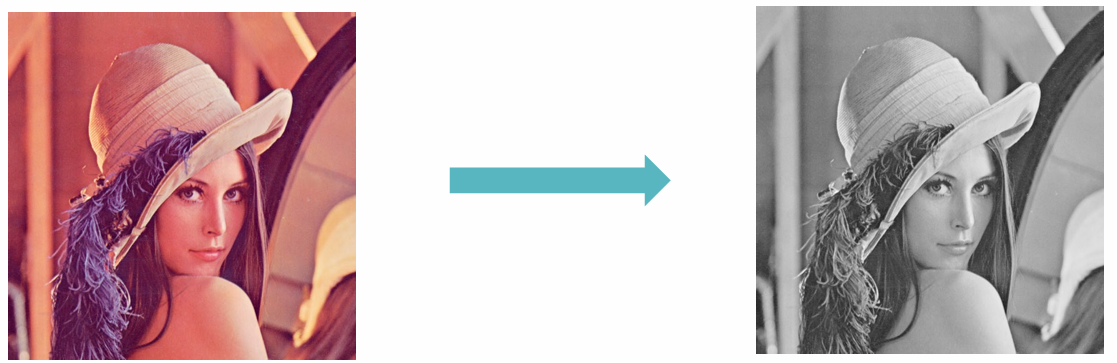
\includegraphics[width=0.7\textwidth]{figuresP/lesson_parallel_4_pag_19.png}
\end{center}

Assume you want to convert an image from RGB (where you have the colour code for each pixel) to greyscale. RGB is a standard to define the quantity of red, green, and blue in each pixel. A greyscale image is an image in which the value of each pixel carries only intensity information. For each pixel (I, J), the conversion formula is: $\text{grey\_Pixel}[I,J] = 0.21*r + 0.71*g + 0.07*b$. We multiply by floating point constants to perform the rescaling and store it. 

The following code contains the kernel i.e. the instructions that each thread must execute. In the main code there will be a part dedicated to copying the data from the host to the device and one that defines the number of threads that have to run the processing. Of course, since the small scheduler has limited dimensions, different multiprocessors might run different blocks, which in this case will correspond to different parts of the image. 

\begin{Verbatim}[label=\makebox{\url{https://github.com/lucabaldini/cmepda/tree/master/slides/latex/snippets/cuda_rgb_to_grayscale.cu}},commandchars=\\\{\}]
\PY{c+cp}{\#}\PY{c+cp}{define CHANNELS 3}

\PY{c+c1}{// GPU Kernel to convert RGB image to Grayscale}
\PY{k+kr}{\_\_global\_\_}\PY{+w}{ }\PY{k+kt}{void}\PY{+w}{ }\PY{n}{colorConvert}\PY{p}{(}\PY{k+kt}{unsigned}\PY{+w}{ }\PY{k+kt}{char}\PY{+w}{ }\PY{o}{*}\PY{+w}{ }\PY{n}{grayImage}\PY{p}{,}
\PY{+w}{                             }\PY{k+kt}{unsigned}\PY{+w}{ }\PY{k+kt}{char}\PY{+w}{ }\PY{o}{*}\PY{+w}{ }\PY{n}{rgbImage}\PY{p}{,}
\PY{+w}{                             }\PY{k+kt}{int}\PY{+w}{ }\PY{n}{width}\PY{p}{,}\PY{+w}{ }\PY{k+kt}{int}\PY{+w}{ }\PY{n}{height}\PY{p}{)}\PY{+w}{ }\PY{p}{\PYZob{}}

\PY{+w}{    }\PY{c+c1}{// Determine the (X, Y) pixel coordinates for this thread}
\PY{+w}{    }\PY{k+kt}{int}\PY{+w}{ }\PY{n}{x}\PY{+w}{ }\PY{o}{=}\PY{+w}{ }\PY{n+nb}{threadIdx}\PY{p}{.}\PY{n}{x}\PY{+w}{ }\PY{o}{+}\PY{+w}{ }\PY{n+nb}{blockIdx}\PY{p}{.}\PY{n}{x}\PY{+w}{ }\PY{o}{*}\PY{+w}{ }\PY{n+nb}{blockDim}\PY{p}{.}\PY{n}{x}\PY{p}{;}
\PY{+w}{    }\PY{k+kt}{int}\PY{+w}{ }\PY{n}{y}\PY{+w}{ }\PY{o}{=}\PY{+w}{ }\PY{n+nb}{threadIdx}\PY{p}{.}\PY{n}{y}\PY{+w}{ }\PY{o}{+}\PY{+w}{ }\PY{n+nb}{blockIdx}\PY{p}{.}\PY{n}{y}\PY{+w}{ }\PY{o}{*}\PY{+w}{ }\PY{n+nb}{blockDim}\PY{p}{.}\PY{n}{y}\PY{p}{;}

\PY{+w}{    }\PY{c+c1}{// Boundary check to prevent accessing memory outside the image}
\PY{+w}{    }\PY{k}{if}\PY{+w}{ }\PY{p}{(}\PY{n}{x}\PY{+w}{ }\PY{o}{\PYZlt{}}\PY{+w}{ }\PY{n}{width}\PY{+w}{ }\PY{o}{\PYZam{}}\PY{o}{\PYZam{}}\PY{+w}{ }\PY{n}{y}\PY{+w}{ }\PY{o}{\PYZlt{}}\PY{+w}{ }\PY{n}{height}\PY{p}{)}\PY{+w}{ }\PY{p}{\PYZob{}}

\PY{+w}{        }\PY{c+c1}{// Convert 2D coordinates to a 1D array index for the grayscale image}
\PY{+w}{        }\PY{k+kt}{int}\PY{+w}{ }\PY{n}{grayOffset}\PY{+w}{ }\PY{o}{=}\PY{+w}{ }\PY{n}{y}\PY{+w}{ }\PY{o}{*}\PY{+w}{ }\PY{n}{width}\PY{+w}{ }\PY{o}{+}\PY{+w}{ }\PY{n}{x}\PY{p}{;}

\PY{+w}{        }\PY{c+c1}{// Calculate the corresponding index in the RGB array (3 values per pixel)}
\PY{+w}{        }\PY{k+kt}{int}\PY{+w}{ }\PY{n}{rgbOffset}\PY{+w}{ }\PY{o}{=}\PY{+w}{ }\PY{n}{grayOffset}\PY{+w}{ }\PY{o}{*}\PY{+w}{ }\PY{n}{CHANNELS}\PY{p}{;}

\PY{+w}{        }\PY{c+c1}{// Extract Red, Green, and Blue channels (adjacent in memory)}
\PY{+w}{        }\PY{k+kt}{unsigned}\PY{+w}{ }\PY{k+kt}{char}\PY{+w}{ }\PY{n}{r}\PY{+w}{ }\PY{o}{=}\PY{+w}{ }\PY{n}{rgbImage}\PY{p}{[}\PY{n}{rgbOffset}\PY{+w}{    }\PY{p}{]}\PY{p}{;}
\PY{+w}{        }\PY{k+kt}{unsigned}\PY{+w}{ }\PY{k+kt}{char}\PY{+w}{ }\PY{n}{g}\PY{+w}{ }\PY{o}{=}\PY{+w}{ }\PY{n}{rgbImage}\PY{p}{[}\PY{n}{rgbOffset}\PY{+w}{ }\PY{o}{+}\PY{+w}{ }\PY{l+m+mi}{1}\PY{p}{]}\PY{p}{;}
\PY{+w}{        }\PY{k+kt}{unsigned}\PY{+w}{ }\PY{k+kt}{char}\PY{+w}{ }\PY{n}{b}\PY{+w}{ }\PY{o}{=}\PY{+w}{ }\PY{n}{rgbImage}\PY{p}{[}\PY{n}{rgbOffset}\PY{+w}{ }\PY{o}{+}\PY{+w}{ }\PY{l+m+mi}{2}\PY{p}{]}\PY{p}{;}

\PY{+w}{        }\PY{c+c1}{// Apply luminance formula to convert RGB to a single grayscale value}
\PY{+w}{        }\PY{n}{grayImage}\PY{p}{[}\PY{n}{grayOffset}\PY{p}{]}\PY{+w}{ }\PY{o}{=}\PY{+w}{ }\PY{p}{(}\PY{k+kt}{unsigned}\PY{+w}{ }\PY{k+kt}{char}\PY{p}{)}\PY{p}{(}\PY{l+m+mf}{0.21f}\PY{o}{*}\PY{n}{r}\PY{+w}{ }\PY{o}{+}\PY{+w}{ }\PY{l+m+mf}{0.71f}\PY{o}{*}\PY{n}{g}\PY{+w}{ }\PY{o}{+}\PY{+w}{ }\PY{l+m+mf}{0.07f}\PY{o}{*}\PY{n}{b}\PY{p}{)}\PY{p}{;}
\PY{+w}{    }\PY{p}{\PYZcb{}}
\PY{p}{\PYZcb{}}
\end{Verbatim}

\subsubsection{- GPUs and images: Blurring an image}
\begin{center}
    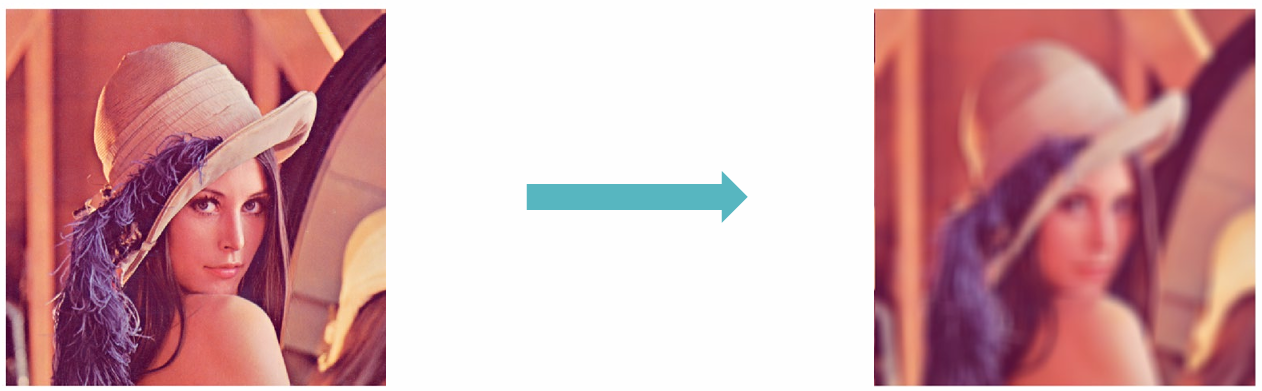
\includegraphics[width=0.7\textwidth]{figuresP/lesson_parallel_4_pag_21.png}
\end{center}

Assume you want to blur an image. In this case, each thread defines a blurring box then the blurring comes from averaging the pixels in the box. Note that in these last 2 cases single threads execute operations on one pixel: there is not a 1 to 1 correspondence between pixels and single processors, but that is obviously not necessary. 

\begin{Verbatim}[label=\makebox{\url{https://github.com/lucabaldini/cmepda/tree/master/slides/latex/snippets/cuda_box_blur.cu}},commandchars=\\\{\}]
\PY{c+cp}{\#}\PY{c+cp}{define BLUR\_SIZE 1}

\PY{c+c1}{// GPU Kernel to apply a Box Blur filter to an image}
\PY{k+kr}{\_\_global\_\_}
\PY{k+kt}{void}\PY{+w}{ }\PY{n}{blurKernel}\PY{p}{(}\PY{k+kt}{unsigned}\PY{+w}{ }\PY{k+kt}{char}\PY{+w}{ }\PY{o}{*}\PY{+w}{ }\PY{n}{in}\PY{p}{,}\PY{+w}{ }\PY{k+kt}{unsigned}\PY{+w}{ }\PY{k+kt}{char}\PY{+w}{ }\PY{o}{*}\PY{+w}{ }\PY{n}{out}\PY{p}{,}\PY{+w}{ }\PY{k+kt}{int}\PY{+w}{ }\PY{n}{w}\PY{p}{,}\PY{+w}{ }\PY{k+kt}{int}\PY{+w}{ }\PY{n}{h}\PY{p}{)}\PY{+w}{ }\PY{p}{\PYZob{}}

\PY{+w}{    }\PY{c+c1}{// Determine the (X, Y) pixel coordinates for this thread}
\PY{+w}{    }\PY{k+kt}{int}\PY{+w}{ }\PY{n}{Col}\PY{+w}{ }\PY{o}{=}\PY{+w}{ }\PY{n+nb}{blockIdx}\PY{p}{.}\PY{n}{x}\PY{+w}{ }\PY{o}{*}\PY{+w}{ }\PY{n+nb}{blockDim}\PY{p}{.}\PY{n}{x}\PY{+w}{ }\PY{o}{+}\PY{+w}{ }\PY{n+nb}{threadIdx}\PY{p}{.}\PY{n}{x}\PY{p}{;}
\PY{+w}{    }\PY{k+kt}{int}\PY{+w}{ }\PY{n}{Row}\PY{+w}{ }\PY{o}{=}\PY{+w}{ }\PY{n+nb}{blockIdx}\PY{p}{.}\PY{n}{y}\PY{+w}{ }\PY{o}{*}\PY{+w}{ }\PY{n+nb}{blockDim}\PY{p}{.}\PY{n}{y}\PY{+w}{ }\PY{o}{+}\PY{+w}{ }\PY{n+nb}{threadIdx}\PY{p}{.}\PY{n}{y}\PY{p}{;}

\PY{+w}{    }\PY{c+c1}{// Boundary check for the main pixel}
\PY{+w}{    }\PY{k}{if}\PY{+w}{ }\PY{p}{(}\PY{n}{Col}\PY{+w}{ }\PY{o}{\PYZlt{}}\PY{+w}{ }\PY{n}{w}\PY{+w}{ }\PY{o}{\PYZam{}}\PY{o}{\PYZam{}}\PY{+w}{ }\PY{n}{Row}\PY{+w}{ }\PY{o}{\PYZlt{}}\PY{+w}{ }\PY{n}{h}\PY{p}{)}\PY{+w}{ }\PY{p}{\PYZob{}}
\PY{+w}{        }\PY{k+kt}{int}\PY{+w}{ }\PY{n}{pixVal}\PY{+w}{ }\PY{o}{=}\PY{+w}{ }\PY{l+m+mi}{0}\PY{p}{;}
\PY{+w}{        }\PY{k+kt}{int}\PY{+w}{ }\PY{n}{pixels}\PY{+w}{ }\PY{o}{=}\PY{+w}{ }\PY{l+m+mi}{0}\PY{p}{;}

\PY{+w}{        }\PY{c+c1}{// Loop over a local window/box centered around the current pixel}
\PY{+w}{        }\PY{k}{for}\PY{p}{(}\PY{k+kt}{int}\PY{+w}{ }\PY{n}{blurRow}\PY{+w}{ }\PY{o}{=}\PY{+w}{ }\PY{o}{\PYZhy{}}\PY{n}{BLUR\_SIZE}\PY{p}{;}\PY{+w}{ }\PY{n}{blurRow}\PY{+w}{ }\PY{o}{\PYZlt{}}\PY{+w}{ }\PY{n}{BLUR\_SIZE}\PY{o}{+}\PY{l+m+mi}{1}\PY{p}{;}\PY{+w}{ }\PY{o}{+}\PY{o}{+}\PY{n}{blurRow}\PY{p}{)}\PY{+w}{ }\PY{p}{\PYZob{}}
\PY{+w}{            }\PY{k}{for}\PY{p}{(}\PY{k+kt}{int}\PY{+w}{ }\PY{n}{blurCol}\PY{+w}{ }\PY{o}{=}\PY{+w}{ }\PY{o}{\PYZhy{}}\PY{n}{BLUR\_SIZE}\PY{p}{;}\PY{+w}{ }\PY{n}{blurCol}\PY{+w}{ }\PY{o}{\PYZlt{}}\PY{+w}{ }\PY{n}{BLUR\_SIZE}\PY{o}{+}\PY{l+m+mi}{1}\PY{p}{;}\PY{+w}{ }\PY{o}{+}\PY{o}{+}\PY{n}{blurCol}\PY{p}{)}\PY{+w}{ }\PY{p}{\PYZob{}}

\PY{+w}{                }\PY{c+c1}{// Calculate coordinates of the neighbor pixel}
\PY{+w}{                }\PY{k+kt}{int}\PY{+w}{ }\PY{n}{curRow}\PY{+w}{ }\PY{o}{=}\PY{+w}{ }\PY{n}{Row}\PY{+w}{ }\PY{o}{+}\PY{+w}{ }\PY{n}{blurRow}\PY{p}{;}
\PY{+w}{                }\PY{k+kt}{int}\PY{+w}{ }\PY{n}{curCol}\PY{+w}{ }\PY{o}{=}\PY{+w}{ }\PY{n}{Col}\PY{+w}{ }\PY{o}{+}\PY{+w}{ }\PY{n}{blurCol}\PY{p}{;}

\PY{+w}{                }\PY{c+c1}{// Check if the neighbor pixel is actually inside image boundaries}
\PY{+w}{                }\PY{k}{if}\PY{p}{(}\PY{n}{curRow}\PY{+w}{ }\PY{o}{\PYZgt{}}\PY{+w}{ }\PY{l+m+mi}{\PYZhy{}1}\PY{+w}{ }\PY{o}{\PYZam{}}\PY{o}{\PYZam{}}\PY{+w}{ }\PY{n}{curRow}\PY{+w}{ }\PY{o}{\PYZlt{}}\PY{+w}{ }\PY{n}{h}\PY{+w}{ }\PY{o}{\PYZam{}}\PY{o}{\PYZam{}}\PY{+w}{ }\PY{n}{curCol}\PY{+w}{ }\PY{o}{\PYZgt{}}\PY{+w}{ }\PY{l+m+mi}{\PYZhy{}1}\PY{+w}{ }\PY{o}{\PYZam{}}\PY{o}{\PYZam{}}\PY{+w}{ }\PY{n}{curCol}\PY{+w}{ }\PY{o}{\PYZlt{}}\PY{+w}{ }\PY{n}{w}\PY{p}{)}\PY{+w}{ }\PY{p}{\PYZob{}}

\PY{+w}{                    }\PY{c+c1}{// Accumulate neighbor pixel values}
\PY{+w}{                    }\PY{n}{pixVal}\PY{+w}{ }\PY{o}{+}\PY{o}{=}\PY{+w}{ }\PY{n}{in}\PY{p}{[}\PY{n}{curRow}\PY{+w}{ }\PY{o}{*}\PY{+w}{ }\PY{n}{w}\PY{+w}{ }\PY{o}{+}\PY{+w}{ }\PY{n}{curCol}\PY{p}{]}\PY{p}{;}
\PY{+w}{                    }\PY{c+c1}{// Count valid neighbors to compute the average later}
\PY{+w}{                    }\PY{n}{pixels}\PY{o}{+}\PY{o}{+}\PY{p}{;}
\PY{+w}{                }\PY{p}{\PYZcb{}}
\PY{+w}{            }\PY{p}{\PYZcb{}}
\PY{+w}{        }\PY{p}{\PYZcb{}}
\PY{+w}{        }\PY{c+c1}{// Compute the average (blur) and write it to the output image array}
\PY{+w}{        }\PY{n}{out}\PY{p}{[}\PY{n}{Row}\PY{+w}{ }\PY{o}{*}\PY{+w}{ }\PY{n}{w}\PY{+w}{ }\PY{o}{+}\PY{+w}{ }\PY{n}{Col}\PY{p}{]}\PY{+w}{ }\PY{o}{=}\PY{+w}{ }\PY{p}{(}\PY{k+kt}{unsigned}\PY{+w}{ }\PY{k+kt}{char}\PY{p}{)}\PY{p}{(}\PY{n}{pixVal}\PY{+w}{ }\PY{o}{/}\PY{+w}{ }\PY{n}{pixels}\PY{p}{)}\PY{p}{;}
\PY{+w}{    }\PY{p}{\PYZcb{}}
\PY{p}{\PYZcb{}}
\end{Verbatim}

\subsection{CUDA program structure}
From the previous examples, you should have understood the typical structure of a CUDA program:
\begin{itemize}
    \item \textbf{Global Declarations:} Declaration of global variables and device functions.
    \item \textbf{Host Code (\texttt{main()}):} The CPU control flow, which typically involves:
    \begin{itemize}
        \item Allocating memory space on the device (GPU).
        \item Transferring data from the host (CPU) to the device.
        \item Setting up the execution configuration (defining grid and block dimensions).
        \item Calling the kernel (e.g., \texttt{kernelOne<<<grid, block>>>(args...)}).
        \item Transferring the computed results from the device back to the host.
        \item Optionally verifying the output against a golden (host-computed) solution.
    \end{itemize}
    \item \textbf{Device Code (\texttt{\_\_global\_\_ void kernelOne(...)}):} The kernel function executed in parallel on the GPU. It includes the declaration of local and shared variables (automatic variables are transparently assigned to registers or local memory) and the use of \texttt{\_\_syncthreads()} for block-level thread synchronization.
\end{itemize}

\hrulefill

\subsection{Note: Evolution of PC Architectures, from Shared Buses to PCIe}

In older PC architectures, system communication relied on a shared bus system managed by two main chips. The Northbridge connected the three components that required high-speed communication: the CPU, the DRAM, and the video card, ensuring the latter had 1st-class access to the main memory. For instance, older NVIDIA cards connected via the AGP bus, achieving transfer rates of up to 2 GB/s. Conversely, the Southbridge acted as a concentrator for slower I/O devices, such as the ATA Bus. The traditional PCI bus, which was connected to the Southbridge, was initially a shared 33 MHz, 32-bit wide bus with a 132 MB/s peak transfer rate, later evolving to 66 MHz and 64-bit to reach a 528 MB/s peak. However, due to its shared nature and the need for bus arbitration, the upstream bandwidth remained a bottleneck for devices, peaking at around 256 MB/s.

\begin{center}
    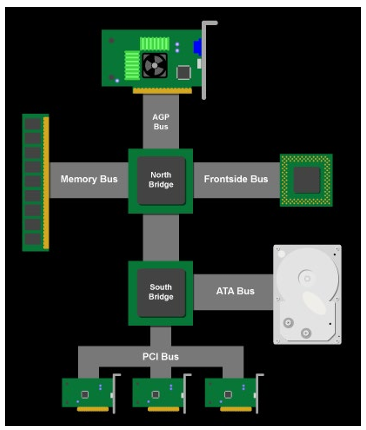
\includegraphics[width=0.4\textwidth]{figuresP/lesson_parallel_4_pag_24.png}
\end{center}

To overcome these limitations, PCI Express (PCIe) was introduced, replacing the shared bus with switched point-to-point serial links across multiple lanes. Because each card now has a dedicated link to a central switch, bus arbitration is completely eliminated. A single PCIe lane is 1-bit wide and consists of 4 wires. In PCIe Gen3, each 2-wire pair can transmit 8 Gb/s in one direction, allowing for simultaneous and symmetric upstream and downstream communication. To maintain signal integrity, data relies on an 8b/10b encoding scheme (where each byte of data is encoded into 10 bits with an equal number of 1's and 0's), yielding a net data rate of approximately 2 Gb/s per lane, each way. By combining multiple lanes into a single link (x1, x2, x4, x8, x12, or x16), bandwidth scales accordingly. Consequently, the net data rates translate to roughly 985 MB/s (x1), 2 GB/s (x2), and 4 GB/s (x4) in each direction.

\begin{center}
    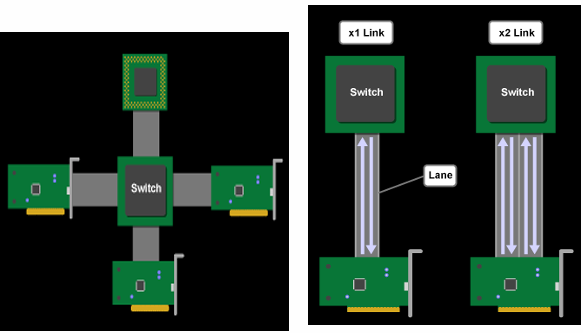
\includegraphics[width=0.8\textwidth]{figuresP/lesson_parallel_4_pag_25.png}
\end{center}

This shift to PCIe significantly altered the overall PC architecture. While earlier systems (up to PCIe Gen2) simply repurposed the North Bridge and South Bridge as PCIe switches, modern architectures integrate both bridges directly into the main processor. Today, while PCIe remains the standard, other specialized fast buses, such as NVLINK, serve as high-performance alternatives for demanding workloads.

\begin{center}
    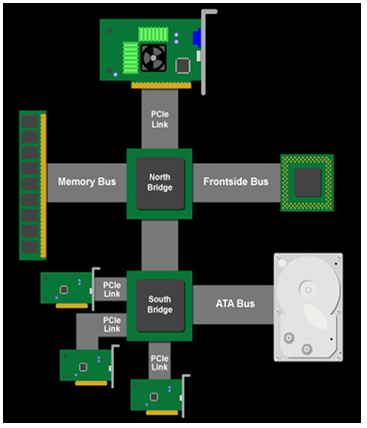
\includegraphics[width=0.4\textwidth]{figuresP/lesson_parallel_4_pag_26.png}
\end{center}

\hrulefill

\begin{minipage}[c]{0.6\textwidth}
    \subsection{The bandwidth problem}
    The bandwidth (and the latency) of the \textit{data transfer between host and device is the main bottleneck of GPU computing} (and also between GPU processor and global memory). This is especially true for massively parallel systems processing massive amounts of data. Tricks like buffering, reordering, and caching can temporarily defy the rules in some cases and modern GPUs will have faster and faster PCIe. Streaming data transfer and processing is a winning strategy to hide latency. Hardware strategies (like DMA, Direct Memory Access) are used to mitigate the data transfer problem, but the concept remains valid: the GPU is made mainly for computation.\\
    That's another aspect you should think about when you are deciding whether to use GPUs or not: if your program needs to access the memory many times, maybe you should actually use a sequential set of instructions. However, if you need to execute a lot of simple instruction on the same set of data, that's when GPUs really shine.
\end{minipage}\hfill 
\begin{minipage}[c]{0.35\textwidth}
    \centering
    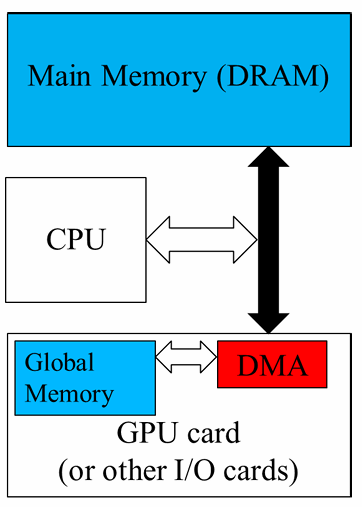
\includegraphics[width=\textwidth]{figuresP/lesson_parallel_4_pag_27.png}
\end{minipage}

\newpage

\section{Hands-on examples for parallel programming}\label{sec:hands_on_cuda_1}
With all that has been said in the last two sections, you may feel overwhelmed by all of these new concepts and methods of GPU programming. Fortunately for you, these last sections of the chapter are all about hands-on examples for parallel programming. As always, feel free to write your own code and experiment with it for as long as you can to become familiar with GPUs.

In the following table, you can find the specifics of the GPU used during the 2025-26 classes.

\begin{center}
    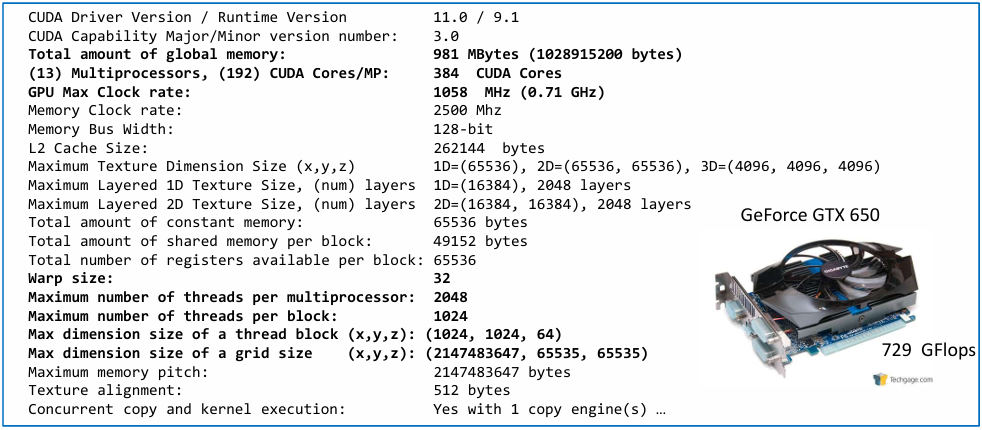
\includegraphics[width=0.9\textwidth]{figuresP/lesson_parallel_4_pag_29.png}
\end{center}

However, I will be using the NVIDIA GeForce MX330 GPU inside my PC to run and modify the code. Its specs are listed in the table below.

\begin{table*}[htbp]
    \centering
    \small
    \begin{tabular}{|ll|}
    \hline
        CUDA Capability Major/Minor version number: & 6.1 \\
        Total amount of global memory: & 2048 MBytes (2147483648 bytes) \\
        (3) Multiprocessors, (128) CUDA Cores/MP: & 384 CUDA Cores \\
        GPU Max Clock rate: & 1594 MHz (1.59 GHz) \\
        Theoretical Peak Performance (FP32): & 1.22 TeraFLOPS \\
        Memory Clock rate: & 3504 MHz \\
        Memory Bus Width: & 64-bit \\
        L2 Cache Size: & 524288 bytes \\
        Total amount of constant memory: & 65536 bytes \\
        Total amount of shared memory per block: & 49152 bytes \\
        Total number of registers available per block: & 65536 \\
        Warp size: & 32 \\
        Maximum number of threads per multiprocessor: & 2048 \\
        Maximum number of threads per block: & 1024 \\
        Max dimension size of a thread block (x,y,z): & (1024, 1024, 64) \\
        Max dimension size of a grid size (x,y,z): & (2147483647, 65535, 65535) \\
        Texture alignment: & 512 bytes \\
        Concurrent copy and kernel execution: & Yes with 1 copy engine(s) \\
    \hline
    \end{tabular}
\end{table*}

In order to try and run the following examples at home, you must have an NVIDIA GPU attached to your PC. If you do have it, then you just need to install the CUDA Toolkit and have fun. Pay attention: you should always check which version of the CUDA Toolkit is compatible with your GPU before installing. However, if you don't have an NVIDIA GPU you can use online resources like Google Colab that let you use a graphics processing unit directly from their platform. 

\subsection{"Hello World!" with Cuda}

Here is our first example of a piece of code running on the GPU:

\begin{Verbatim}[label=\makebox{\url{https://github.com/lucabaldini/cmepda/tree/master/slides/latex/snippets/cuda_hello_world.cu}},commandchars=\\\{\}]
\PY{c+cp}{\#}\PY{c+cp}{include}\PY{+w}{ }\PY{c+cpf}{\PYZlt{}cuda.h\PYZgt{}}
\PY{c+cp}{\#}\PY{c+cp}{include}\PY{+w}{ }\PY{c+cpf}{\PYZlt{}stdio.h\PYZgt{}}

\PY{c+c1}{// The word \PYZdq{}\_\_global\_\_\PYZdq{} is not C standard! You need \#include \PYZlt{}cuda.h\PYZgt{} !}

\PY{c+c1}{// Part of the code running on the GPU: the kernel (with no arguments and no returns)}
\PY{k+kr}{\_\_global\_\_}\PY{+w}{ }\PY{k+kt}{void}\PY{+w}{ }\PY{n}{mykernel}\PY{p}{(}\PY{k+kt}{void}\PY{p}{)}\PY{+w}{ }\PY{p}{\PYZob{}}
\PY{+w}{  }\PY{n}{printf}\PY{p}{(}\PY{l+s}{\PYZdq{}}\PY{l+s}{Hello World from GPU! (block: \PYZpc{}d thread: \PYZpc{}d)}\PY{l+s+se}{\PYZbs{}n}\PY{l+s}{\PYZdq{}}\PY{p}{,}\PY{n+nb}{blockIdx}\PY{p}{.}\PY{n}{x}\PY{p}{,}\PY{n+nb}{threadIdx}\PY{p}{.}\PY{n}{x}\PY{p}{)}\PY{p}{;}
\PY{p}{\PYZcb{}}

\PY{c+c1}{// Part of the code running on the CPU}
\PY{k+kt}{int}\PY{+w}{ }\PY{n}{main}\PY{p}{(}\PY{k+kt}{void}\PY{p}{)}\PY{+w}{ }\PY{p}{\PYZob{}}
\PY{+w}{  }\PY{c+c1}{// I\PYZsq{}m using 5 blocks with 2 threads per block to run the kernel}
\PY{+w}{  }\PY{n}{mykernel}\PY{+w}{ }\PY{o}{\PYZlt{}}\PY{o}{\PYZlt{}}\PY{o}{\PYZlt{}}\PY{l+m+mi}{5}\PY{p}{,}\PY{l+m+mi}{2}\PY{o}{\PYZgt{}}\PY{o}{\PYZgt{}}\PY{o}{\PYZgt{}}\PY{p}{(}\PY{p}{)}\PY{p}{;}
\PY{+w}{  }\PY{n}{cudaDeviceSynchronize}\PY{p}{(}\PY{p}{)}\PY{p}{;}
\PY{+w}{  }\PY{n}{printf}\PY{p}{(}\PY{l+s}{\PYZdq{}}\PY{l+s}{Hello World from Host!}\PY{l+s+se}{\PYZbs{}n}\PY{l+s}{\PYZdq{}}\PY{p}{)}\PY{p}{;}
\PY{+w}{  }\PY{k}{return}\PY{+w}{ }\PY{l+m+mi}{0}\PY{p}{;}
\PY{p}{\PYZcb{}}

[Output]
Hello World from GPU! (block: 3 thread: 0)                                                                      
Hello World from GPU! (block: 3 thread: 1)
Hello World from GPU! (block: 0 thread: 0)
Hello World from GPU! (block: 0 thread: 1)
Hello World from GPU! (block: 4 thread: 0)
Hello World from GPU! (block: 4 thread: 1)
Hello World from GPU! (block: 1 thread: 0)
Hello World from GPU! (block: 1 thread: 1)
Hello World from GPU! (block: 2 thread: 0)
Hello World from GPU! (block: 2 thread: 1)
Hello World from Host!
\end{Verbatim}

As you can see, this is very similar to a standard C code. You have your \texttt{main} function and your standard \texttt{\#include <stdio.h>} that lets you use your \texttt{printf} function. \\ However, the term \texttt{\_\_global\_\_} is not C standard and is imported using \texttt{\#include <cuda.h>}. The \texttt{\_\_global\_\_} execution space specifier tells the compiler that this is a \textit{kernel} function which, as we said before, is a function executed on the GPU but called from the host. In this case, it has no parameters and no returns, as specified by the use of \texttt{void}. \\ 
The command \texttt{cudaDeviceSynchronize()} is crucial. In CUDA, kernel launches are \textit{asynchronous}: the CPU issues the command to start the kernel and immediately moves to the next instruction without waiting for the GPU. \\
\texttt{blockIdx.x} and \texttt{threadIdx.x} identify the block and the thread that are running the code, as you can see in the return. \\
\texttt{cudaDeviceSynchronize()} forces the CPU to halt and wait until all GPU tasks are completely finished, ensuring the GPU's print statements are processed before the program ends. Try and comment this line to see what happens.

Now, how do we run this? First of all, you need to compile it using the CUDA compiler called \textbf{NVCC}, which will be automatically installed with the Toolkit. On Windows you must run \\
\texttt{nvcc HelloWorldGpu.cu -o HelloWorldGpu.exe} \\ 
\footnote{Depending on your GPU's physical architecture and your CUDA Toolkit version, you might need to specify the target architecture during compilation using the \texttt{-arch} flag (e.g., \texttt{-arch=sm\_61} for Pascal-based GPUs like the MX330 or GTX 10-series). This is because newer versions of the CUDA compiler periodically drop support for older GPU architectures. If you encounter an "Unsupported gpu architecture" error, you will need to either append this flag or install an older, compatible version of the Toolkit.} 
(you can input whatever name you want for the executable file after the \texttt{-o}) and then \\
\texttt{.\textbackslash HelloWorldGpu.exe} \\
to actually execute the code. On Linux it is all very similar: \\
\texttt{nvcc HelloWorldGpu.cu -o HelloWorldGpu} \\
\texttt{./HelloWorldGpu}

Note that it is not always true that block 0 is executed before block 1 and so on: the big scheduler can organize the execution in a way that can appear non sequential (Of course! It's parallel computing!). In our case, the "strange" output is due to the fact that we asked the GPU to run 5 blocks of code when it only contains 3 multiprocessors \footnote{That is not actually true for our simple \texttt{printf} function, but let's pretend}. The same thing could happen with threads, and the effect could have been clear if I had written a code with more than 128 threads per block. You can actually force the GPU to execute blocks and threads in a precise order, but that will probably slow down your execution. 

\subsection{Vector sum: CUDA vs. C}
Take a look at the following example. It is a simple serial code that runs entirely on the CPU (CUDA is used exclusively to measure the execution time). Here's what it does in detail:

\begin{itemize}
    \item[-] The \texttt{RandomVector} function (lines 6-10) initializes an array with random integers between 1 and 100. 
    
    \item[-] The \texttt{VecAddSerial} (lines 13-17) function performs a standard element-by-element vector addition on the CPU using a simple \texttt{for} loop.
    
    \item[-] Inside the \texttt{main} function, standard C \texttt{malloc} (lines 29-31) is used to allocate memory on the host (CPU) for three large vectors of size $N = 1048576$ elements.
    
    \item[-] The program leverages the CUDA to measure the elapsed time. It declares two events of type \texttt{cudaEvent\_t} (\texttt{start} and \texttt{stop}) and creates them using \texttt{cudaEventCreate} (lines 24-26).
    
    \item[-] \texttt{cudaEventRecord(start)} marks the beginning of the timer then \texttt{VecAddSerial(h\_a, h\_b, h\_c)} executes the addition entirely on the CPU and \texttt{cudaEventRecord(stop)} marks the end of the operation (lines 36-43).
    
    \item[-] \texttt{cudaEventSynchronize(stop)} (line 43) is called to ensure that all operations associated with the \texttt{stop} event are fully completed before proceeding. 
    
    \item[-] \texttt{cudaEventElapsedTime} (line 44) calculates the time difference between the events in ms. 
    
    \item[-] Finally, the result is printed to the console\footnote{In reality the output will change every time you execute the code, but not by much. The output below is a reference value, and so will be the time measures in the next examples.}, and the host memory is released using \texttt{free()} (lines 47-52).
\end{itemize}

\begin{Verbatim}[label=\makebox{\url{https://github.com/lucabaldini/cmepda/tree/master/slides/latex/snippets/cuda_vec_add_serial.cu}},commandchars=\\\{\}]
\PY{c+cp}{\#}\PY{c+cp}{include}\PY{+w}{ }\PY{c+cpf}{\PYZlt{}stdio.h\PYZgt{}}
\PY{c+cp}{\#}\PY{c+cp}{include}\PY{+w}{ }\PY{c+cpf}{\PYZlt{}stdlib.h\PYZgt{}}\PY{c+c1}{ // Added for rand() and malloc()}
\PY{c+cp}{\#}\PY{c+cp}{define N 1048576}

\PY{c+c1}{// Function to define a vector with N elements (with N\PYZgt{}10\PYZca{}6)}
\PY{k+kt}{void}\PY{+w}{ }\PY{n+nf}{RandomVector}\PY{p}{(}\PY{k+kt}{int}\PY{+w}{ }\PY{o}{*}\PY{n}{a}\PY{p}{,}\PY{+w}{ }\PY{k+kt}{int}\PY{+w}{ }\PY{n}{nn}\PY{p}{)}\PY{p}{\PYZob{}}
\PY{+w}{  }\PY{k}{for}\PY{+w}{ }\PY{p}{(}\PY{k+kt}{int}\PY{+w}{ }\PY{n}{i}\PY{o}{=}\PY{l+m+mi}{0}\PY{p}{;}\PY{n}{i}\PY{o}{\PYZlt{}}\PY{n}{nn}\PY{p}{;}\PY{n}{i}\PY{o}{+}\PY{o}{+}\PY{p}{)}\PY{+w}{ }\PY{p}{\PYZob{}}
\PY{+w}{    }\PY{n}{a}\PY{p}{[}\PY{n}{i}\PY{p}{]}\PY{o}{=}\PY{n}{rand}\PY{p}{(}\PY{p}{)}\PY{o}{\PYZpc{}}\PY{l+m+mi}{100}\PY{o}{+}\PY{l+m+mi}{1}\PY{p}{;}
\PY{+w}{  }\PY{p}{\PYZcb{}}
\PY{p}{\PYZcb{}}

\PY{c+c1}{// Function to add 2 vectors using a for cycle}
\PY{k+kt}{void}\PY{+w}{ }\PY{n+nf}{VecAddSerial}\PY{p}{(}\PY{k+kt}{int}\PY{+w}{ }\PY{o}{*}\PY{n}{a}\PY{p}{,}\PY{+w}{ }\PY{k+kt}{int}\PY{+w}{ }\PY{o}{*}\PY{n}{b}\PY{p}{,}\PY{+w}{ }\PY{k+kt}{int}\PY{+w}{ }\PY{o}{*}\PY{n}{c}\PY{p}{)}\PY{p}{\PYZob{}}
\PY{+w}{  }\PY{k}{for}\PY{+w}{ }\PY{p}{(}\PY{k+kt}{int}\PY{+w}{ }\PY{n}{i}\PY{o}{=}\PY{l+m+mi}{0}\PY{p}{;}\PY{n}{i}\PY{o}{\PYZlt{}}\PY{n}{N}\PY{p}{;}\PY{n}{i}\PY{o}{+}\PY{o}{+}\PY{p}{)}\PY{p}{\PYZob{}}
\PY{+w}{    }\PY{n}{c}\PY{p}{[}\PY{n}{i}\PY{p}{]}\PY{+w}{ }\PY{o}{=}\PY{+w}{ }\PY{n}{a}\PY{p}{[}\PY{n}{i}\PY{p}{]}\PY{o}{+}\PY{n}{b}\PY{p}{[}\PY{n}{i}\PY{p}{]}\PY{p}{;}
\PY{+w}{  }\PY{p}{\PYZcb{}}
\PY{p}{\PYZcb{}}

\PY{k+kt}{int}\PY{+w}{ }\PY{n+nf}{main}\PY{p}{(}\PY{k+kt}{void}\PY{p}{)}\PY{+w}{ }\PY{p}{\PYZob{}}
\PY{+w}{  }\PY{k+kt}{int}\PY{+w}{ }\PY{o}{*}\PY{n}{h\_a}\PY{p}{,}\PY{+w}{ }\PY{o}{*}\PY{n}{h\_b}\PY{p}{,}\PY{+w}{ }\PY{o}{*}\PY{n}{h\_c}\PY{p}{;}
\PY{+w}{  }\PY{k+kt}{int}\PY{+w}{ }\PY{n}{size}\PY{+w}{ }\PY{o}{=}\PY{+w}{ }\PY{n}{N}\PY{o}{*}\PY{k}{sizeof}\PY{p}{(}\PY{k+kt}{int}\PY{p}{)}\PY{p}{;}

\PY{+w}{  }\PY{k+kt}{float}\PY{+w}{ }\PY{n}{time}\PY{p}{;}
\PY{+w}{  }\PY{n}{cudaEvent\_t}\PY{+w}{ }\PY{n}{start}\PY{p}{,}\PY{n}{stop}\PY{p}{;}
\PY{+w}{  }\PY{n}{cudaEventCreate}\PY{p}{(}\PY{o}{\PYZam{}}\PY{n}{start}\PY{p}{)}\PY{p}{;}
\PY{+w}{  }\PY{n}{cudaEventCreate}\PY{p}{(}\PY{o}{\PYZam{}}\PY{n}{stop}\PY{p}{)}\PY{p}{;}

\PY{+w}{  }\PY{c+c1}{// Allocation of a memory space in the host for the 2 vectors (and filling)}
\PY{+w}{  }\PY{n}{h\_a}\PY{+w}{ }\PY{o}{=}\PY{+w}{ }\PY{p}{(}\PY{k+kt}{int}\PY{+w}{ }\PY{o}{*}\PY{p}{)}\PY{n}{malloc}\PY{p}{(}\PY{n}{size}\PY{p}{)}\PY{p}{;}
\PY{+w}{  }\PY{n}{h\_b}\PY{+w}{ }\PY{o}{=}\PY{+w}{ }\PY{p}{(}\PY{k+kt}{int}\PY{+w}{ }\PY{o}{*}\PY{p}{)}\PY{n}{malloc}\PY{p}{(}\PY{n}{size}\PY{p}{)}\PY{p}{;}
\PY{+w}{  }\PY{n}{h\_c}\PY{+w}{ }\PY{o}{=}\PY{+w}{ }\PY{p}{(}\PY{k+kt}{int}\PY{+w}{ }\PY{o}{*}\PY{p}{)}\PY{n}{malloc}\PY{p}{(}\PY{n}{size}\PY{p}{)}\PY{p}{;}
\PY{+w}{  }\PY{n}{RandomVector}\PY{p}{(}\PY{n}{h\_a}\PY{p}{,}\PY{n}{N}\PY{p}{)}\PY{p}{;}
\PY{+w}{  }\PY{n}{RandomVector}\PY{p}{(}\PY{n}{h\_b}\PY{p}{,}\PY{n}{N}\PY{p}{)}\PY{p}{;}

\PY{+w}{  }\PY{c+c1}{// Start time}
\PY{+w}{  }\PY{n}{cudaEventRecord}\PY{p}{(}\PY{n}{start}\PY{p}{)}\PY{p}{;}

\PY{+w}{  }\PY{c+c1}{//Launch serial sum on CPU}
\PY{+w}{  }\PY{n}{VecAddSerial}\PY{p}{(}\PY{n}{h\_a}\PY{p}{,}\PY{n}{h\_b}\PY{p}{,}\PY{n}{h\_c}\PY{p}{)}\PY{p}{;}

\PY{+w}{  }\PY{c+c1}{// Stop time}
\PY{+w}{  }\PY{n}{cudaEventRecord}\PY{p}{(}\PY{n}{stop}\PY{p}{)}\PY{p}{;}
\PY{+w}{  }\PY{n}{cudaEventSynchronize}\PY{p}{(}\PY{n}{stop}\PY{p}{)}\PY{p}{;}
\PY{+w}{  }\PY{n}{cudaEventElapsedTime}\PY{p}{(}\PY{o}{\PYZam{}}\PY{n}{time}\PY{p}{,}\PY{+w}{ }\PY{n}{start}\PY{p}{,}\PY{+w}{ }\PY{n}{stop}\PY{p}{)}\PY{p}{;}

\PY{+w}{  }\PY{c+c1}{// Print time}
\PY{+w}{  }\PY{n}{printf}\PY{p}{(}\PY{l+s}{\PYZdq{}}\PY{l+s}{Time: \PYZpc{}3.5f ms}\PY{l+s+se}{\PYZbs{}n}\PY{l+s}{\PYZdq{}}\PY{p}{,}\PY{n}{time}\PY{p}{)}\PY{p}{;}

\PY{+w}{  }\PY{c+c1}{// Cleanup}
\PY{+w}{  }\PY{n}{free}\PY{p}{(}\PY{n}{h\_a}\PY{p}{)}\PY{p}{;}
\PY{+w}{  }\PY{n}{free}\PY{p}{(}\PY{n}{h\_b}\PY{p}{)}\PY{p}{;}
\PY{+w}{  }\PY{n}{free}\PY{p}{(}\PY{n}{h\_c}\PY{p}{)}\PY{p}{;}

\PY{+w}{  }\PY{k}{return}\PY{p}{(}\PY{l+m+mi}{0}\PY{p}{)}\PY{p}{;}
\PY{p}{\PYZcb{}}

[Output]
Time: 4.34893 ms
\end{Verbatim}

Now we should try and parallelize our computation. At first glance this next example seems to do just that. \\ The \texttt{VecAddGpu} kernel (lines 13-15) is executed by the GPU and it should speed up the process. Note that in order to use the kernel, the program copies the vectors defined in the host memory (\texttt{h\_a}, \texttt{h\_b}, \texttt{h\_c}) to the device memory (\texttt{d\_a}, \texttt{d\_b}, \texttt{d\_c}) using \texttt{cudaMalloc} and \texttt{cudaMemcpy} (lines 35-41). Also, it copies the result of the computation back to the host (line 56).

\input{pygments/Cuda_VecAdd_Blocks}

\begin{figure}[htbp]
    \begin{minipage}[c]{0.55\textwidth}
    Now, if you take a look at the output, it surely isn't optimal: the execution time has more than doubled. As said, the act of moving data from host to device and vice versa might slow down our execution, but in this case the problem is elsewhere, and once you notice it, it is pretty obvious. 
    \newline\newline Take a look at line 48:\\
    \texttt{VecAddGpu<<<1,N>>>(d\_a,d\_b,d\_c);} \\
    It is saying that we are running more than a million blocks with a single thread per block (as represented in figure)! Each of the 3 multiprocessors in our GPU is running a block, but only one of its cores (which is slower than the CPU),is actually working, while the other 127 are doing nothing! That is not parallelization, it is a waste of computing power.
    \end{minipage}\hfill 
    \begin{minipage}[c]{0.4\textwidth}
        \centering
        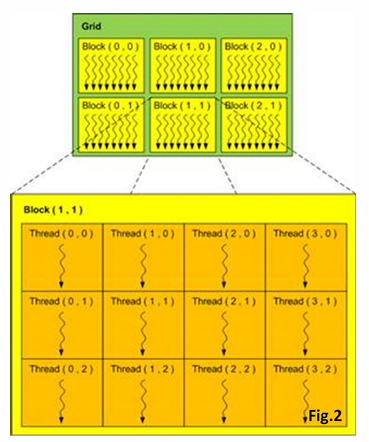
\includegraphics[width=\textwidth]{figuresP/lesson_parallel_4_pag_33.png}
    \end{minipage}
\end{figure} 

We could also ask ourselves what would happen if instead we tried to divide the computation in a million threads inside the same block. That's fairly easy to implement: just rewrite the kernel (lines 13-15) as such
\begin{Verbatim}[commandchars=\\\{\}]
\PY{k+kr}{\_\_global\_\_}\PY{+w}{ }\PY{k+kt}{void}\PY{+w}{ }\PY{n}{VecAddGpu}\PY{p}{(}\PY{k+kt}{int}\PY{+w}{ }\PY{o}{*}\PY{n}{a}\PY{p}{,}\PY{+w}{ }\PY{k+kt}{int}\PY{+w}{ }\PY{o}{*}\PY{n}{b}\PY{p}{,}\PY{+w}{ }\PY{k+kt}{int}\PY{+w}{ }\PY{o}{*}\PY{n}{c}\PY{p}{)}\PY{p}{\PYZob{}}
\PY{+w}{  }\PY{n}{c}\PY{p}{[}\PY{n+nb}{threadIdx}\PY{p}{.}\PY{n}{x}\PY{p}{]}\PY{+w}{ }\PY{o}{=}\PY{+w}{ }\PY{n}{a}\PY{p}{[}\PY{n+nb}{threadIdx}\PY{p}{.}\PY{n}{x}\PY{p}{]}\PY{o}{+}\PY{n}{b}\PY{p}{[}\PY{n+nb}{threadIdx}\PY{p}{.}\PY{n}{x}\PY{p}{]}\PY{p}{;}
\PY{p}{\PYZcb{}}
\end{Verbatim}
and launch it with (line 47)
\begin{Verbatim}[commandchars=\\\{\}]
\PY{n}{VecAddGpu}\PY{o}{\PYZlt{}}\PY{o}{\PYZlt{}}\PY{o}{\PYZlt{}}\PY{l+m+mi}{1}\PY{p}{,}\PY{n}{N}\PY{o}{\PYZgt{}}\PY{o}{\PYZgt{}}\PY{o}{\PYZgt{}}\PY{p}{(}\PY{n}{d\_a}\PY{p}{,}\PY{n}{d\_b}\PY{p}{,}\PY{n}{d\_c}\PY{p}{)}\PY{p}{;}
\end{Verbatim}
In my own device the output is \texttt{Time: 0.15997 ms}. That seems wonderful, a speed-up of about 40 with respect to the serial code. However, something is wrong and you can check it in 2 ways:
\begin{itemize}
\item[-] Try to print your result (maybe not all the million or so elements of \texttt{h\_c}, but the first 2 or 3 hundred): you will find that they are all equal to zero. 
\item[-] After the stop time instruction, "ask" CUDA if an error was found (this is the best practice) using 
\begin{Verbatim}[commandchars=\\\{\}]
\PY{n}{cudaError\_t}\PY{+w}{ }\PY{n}{KernelError}\PY{+w}{ }\PY{o}{=}\PY{+w}{ }\PY{n}{cudaGetLastError}\PY{p}{(}\PY{p}{)}\PY{p}{;}
\PY{n}{printf}\PY{p}{(}\PY{l+s}{\PYZdq{}}\PY{l+s}{Error: \PYZpc{}s}\PY{l+s+se}{\PYZbs{}n}\PY{l+s}{\PYZdq{}}\PY{p}{,}\PY{+w}{ }\PY{n}{cudaGetErrorString}\PY{p}{(}\PY{n}{KernelError}\PY{p}{)}\PY{p}{)}\PY{p}{;}
\end{Verbatim}
Your output should read \texttt{Error: invalid configuration argument}.
\end{itemize}
Go back to the specifics of our GPU: the maximum number of threads per block is 1024, which is way lower with respect to the million elements of the vector. Our device cannot execute our instructions! 

That should teach you an important lesson: \textbf{a serial code is much more portable than a parallel one}. In other words, the way you run your programs is much more dependent on the machine you are running them on if you are using the GPU instead of the simple CPU. Before starting to work on the device instead of the host, you must always be aware of its characteristics. 

Now no more tricks: down here you will find how you should really write this code in order to make it parallel. \\Note that we are using 128 threads per block. Even if the maximum number of threads per block is 1024, we know that our GPU has 128 cores per multiprocessor. For this reason, in this kind of operation, we won't have a significant speed up using a number of threads higher than 128. \\ Look at the kernel (the variable \texttt{blockDim.x} is the dimensions of the block, that in this case is equal to 128) and how it is launched: the number of blocks is equal to number of elements in the vectors divided by the number of threads per block (of course!). The output tells us that we obtained a code that is 10 times faster than the serial version and without any errors during the GPU computation. Success!

\begin{Verbatim}[label=\makebox{\url{https://github.com/lucabaldini/cmepda/tree/master/slides/latex/snippets/cuda_vec_add_complete.cu}},commandchars=\\\{\}]
\PY{c+cp}{\#}\PY{c+cp}{include}\PY{+w}{ }\PY{c+cpf}{\PYZlt{}stdio.h\PYZgt{}}
\PY{c+cp}{\#}\PY{c+cp}{include}\PY{+w}{ }\PY{c+cpf}{\PYZlt{}stdlib.h\PYZgt{}}
\PY{c+cp}{\#}\PY{c+cp}{define N 1048576}
\PY{c+cp}{\#}\PY{c+cp}{define THREADS\_PER\_BLOCK 128}

\PY{c+c1}{// Function to define a vector with N elements (with N\PYZgt{}10\PYZca{}6)}
\PY{k+kt}{void}\PY{+w}{ }\PY{n+nf}{RandomVector}\PY{p}{(}\PY{k+kt}{int}\PY{+w}{ }\PY{o}{*}\PY{n}{a}\PY{p}{,}\PY{+w}{ }\PY{k+kt}{int}\PY{+w}{ }\PY{n}{nn}\PY{p}{)}\PY{p}{\PYZob{}}
\PY{+w}{  }\PY{k}{for}\PY{+w}{ }\PY{p}{(}\PY{k+kt}{int}\PY{+w}{ }\PY{n}{i}\PY{o}{=}\PY{l+m+mi}{0}\PY{p}{;}\PY{n}{i}\PY{o}{\PYZlt{}}\PY{n}{nn}\PY{p}{;}\PY{n}{i}\PY{o}{+}\PY{o}{+}\PY{p}{)}\PY{+w}{ }\PY{p}{\PYZob{}}
\PY{+w}{    }\PY{n}{a}\PY{p}{[}\PY{n}{i}\PY{p}{]}\PY{o}{=}\PY{n}{rand}\PY{p}{(}\PY{p}{)}\PY{o}{\PYZpc{}}\PY{l+m+mi}{100}\PY{o}{+}\PY{l+m+mi}{1}\PY{p}{;}
\PY{+w}{  }\PY{p}{\PYZcb{}}
\PY{p}{\PYZcb{}}

\PY{c+c1}{// Kernel to add 2 vectors using the GPU}
\PY{k+kr}{\_\_global\_\_}\PY{+w}{ }\PY{k+kt}{void}\PY{+w}{ }\PY{n}{VecAddGpu}\PY{p}{(}\PY{k+kt}{int}\PY{+w}{ }\PY{o}{*}\PY{n}{a}\PY{p}{,}\PY{+w}{ }\PY{k+kt}{int}\PY{+w}{ }\PY{o}{*}\PY{n}{b}\PY{p}{,}\PY{+w}{ }\PY{k+kt}{int}\PY{+w}{ }\PY{o}{*}\PY{n}{c}\PY{p}{)}\PY{p}{\PYZob{}}
\PY{+w}{  }\PY{k+kt}{int}\PY{+w}{ }\PY{n}{index}\PY{+w}{ }\PY{o}{=}\PY{+w}{ }\PY{n+nb}{threadIdx}\PY{p}{.}\PY{n}{x}\PY{+w}{ }\PY{o}{+}\PY{+w}{ }\PY{n+nb}{blockIdx}\PY{p}{.}\PY{n}{x}\PY{o}{*}\PY{n+nb}{blockDim}\PY{p}{.}\PY{n}{x}\PY{p}{;}
\PY{+w}{  }\PY{n}{c}\PY{p}{[}\PY{n}{index}\PY{p}{]}\PY{+w}{ }\PY{o}{=}\PY{+w}{ }\PY{n}{a}\PY{p}{[}\PY{n}{index}\PY{p}{]}\PY{o}{+}\PY{n}{b}\PY{p}{[}\PY{n}{index}\PY{p}{]}\PY{p}{;}
\PY{p}{\PYZcb{}}

\PY{k+kt}{int}\PY{+w}{ }\PY{n}{main}\PY{p}{(}\PY{k+kt}{void}\PY{p}{)}\PY{+w}{ }\PY{p}{\PYZob{}}
\PY{+w}{  }\PY{k+kt}{int}\PY{+w}{ }\PY{o}{*}\PY{n}{h\_a}\PY{p}{,}\PY{+w}{ }\PY{o}{*}\PY{n}{h\_b}\PY{p}{,}\PY{+w}{ }\PY{o}{*}\PY{n}{h\_c}\PY{p}{;}
\PY{+w}{  }\PY{k+kt}{int}\PY{+w}{ }\PY{o}{*}\PY{n}{d\_a}\PY{p}{,}\PY{+w}{ }\PY{o}{*}\PY{n}{d\_b}\PY{p}{,}\PY{+w}{ }\PY{o}{*}\PY{n}{d\_c}\PY{p}{;}
\PY{+w}{  }\PY{k+kt}{int}\PY{+w}{ }\PY{n}{size}\PY{+w}{ }\PY{o}{=}\PY{+w}{ }\PY{n}{N}\PY{o}{*}\PY{k}{sizeof}\PY{p}{(}\PY{k+kt}{int}\PY{p}{)}\PY{p}{;}

\PY{+w}{  }\PY{k+kt}{float}\PY{+w}{ }\PY{n}{time}\PY{p}{;}
\PY{+w}{  }\PY{n}{cudaEvent\_t}\PY{+w}{ }\PY{n}{start}\PY{p}{,}\PY{n}{stop}\PY{p}{;}
\PY{+w}{  }\PY{n}{cudaEventCreate}\PY{p}{(}\PY{o}{\PYZam{}}\PY{n}{start}\PY{p}{)}\PY{p}{;}
\PY{+w}{  }\PY{n}{cudaEventCreate}\PY{p}{(}\PY{o}{\PYZam{}}\PY{n}{stop}\PY{p}{)}\PY{p}{;}

\PY{+w}{  }\PY{c+c1}{// Allocation of a memory space in the host for the 2 vectors (and filling)}
\PY{+w}{  }\PY{n}{h\_a}\PY{+w}{ }\PY{o}{=}\PY{+w}{ }\PY{p}{(}\PY{k+kt}{int}\PY{+w}{ }\PY{o}{*}\PY{p}{)}\PY{n}{malloc}\PY{p}{(}\PY{n}{size}\PY{p}{)}\PY{p}{;}
\PY{+w}{  }\PY{n}{h\_b}\PY{+w}{ }\PY{o}{=}\PY{+w}{ }\PY{p}{(}\PY{k+kt}{int}\PY{+w}{ }\PY{o}{*}\PY{p}{)}\PY{n}{malloc}\PY{p}{(}\PY{n}{size}\PY{p}{)}\PY{p}{;}
\PY{+w}{  }\PY{n}{h\_c}\PY{+w}{ }\PY{o}{=}\PY{+w}{ }\PY{p}{(}\PY{k+kt}{int}\PY{+w}{ }\PY{o}{*}\PY{p}{)}\PY{n}{malloc}\PY{p}{(}\PY{n}{size}\PY{p}{)}\PY{p}{;}
\PY{+w}{  }\PY{n}{RandomVector}\PY{p}{(}\PY{n}{h\_a}\PY{p}{,}\PY{n}{N}\PY{p}{)}\PY{p}{;}
\PY{+w}{  }\PY{n}{RandomVector}\PY{p}{(}\PY{n}{h\_b}\PY{p}{,}\PY{n}{N}\PY{p}{)}\PY{p}{;}

\PY{+w}{  }\PY{c+c1}{// Allocation of a memory space in the GPU for the 2 vectors}
\PY{+w}{  }\PY{n}{cudaMalloc}\PY{p}{(}\PY{p}{(}\PY{k+kt}{void}\PY{+w}{ }\PY{o}{*}\PY{o}{*}\PY{p}{)}\PY{o}{\PYZam{}}\PY{n}{d\_a}\PY{p}{,}\PY{+w}{ }\PY{n}{size}\PY{p}{)}\PY{p}{;}
\PY{+w}{  }\PY{n}{cudaMalloc}\PY{p}{(}\PY{p}{(}\PY{k+kt}{void}\PY{+w}{ }\PY{o}{*}\PY{o}{*}\PY{p}{)}\PY{o}{\PYZam{}}\PY{n}{d\_b}\PY{p}{,}\PY{+w}{ }\PY{n}{size}\PY{p}{)}\PY{p}{;}
\PY{+w}{  }\PY{n}{cudaMalloc}\PY{p}{(}\PY{p}{(}\PY{k+kt}{void}\PY{+w}{ }\PY{o}{*}\PY{o}{*}\PY{p}{)}\PY{o}{\PYZam{}}\PY{n}{d\_c}\PY{p}{,}\PY{+w}{ }\PY{n}{size}\PY{p}{)}\PY{p}{;}

\PY{+w}{  }\PY{c+c1}{// Copy input vectors form host to GPU}
\PY{+w}{  }\PY{n}{cudaMemcpy}\PY{p}{(}\PY{n}{d\_a}\PY{p}{,}\PY{+w}{ }\PY{n}{h\_a}\PY{p}{,}\PY{+w}{ }\PY{n}{size}\PY{p}{,}\PY{+w}{ }\PY{n}{cudaMemcpyHostToDevice}\PY{p}{)}\PY{p}{;}
\PY{+w}{  }\PY{n}{cudaMemcpy}\PY{p}{(}\PY{n}{d\_b}\PY{p}{,}\PY{+w}{ }\PY{n}{h\_b}\PY{p}{,}\PY{+w}{ }\PY{n}{size}\PY{p}{,}\PY{+w}{ }\PY{n}{cudaMemcpyHostToDevice}\PY{p}{)}\PY{p}{;}

\PY{+w}{  }\PY{c+c1}{// Start time}
\PY{+w}{  }\PY{n}{cudaEventRecord}\PY{p}{(}\PY{n}{start}\PY{p}{)}\PY{p}{;}

\PY{+w}{  }\PY{c+c1}{// Launch Kernel  on GPU}
\PY{+w}{  }\PY{n}{VecAddGpu}\PY{o}{\PYZlt{}}\PY{o}{\PYZlt{}}\PY{o}{\PYZlt{}}\PY{n}{N}\PY{o}{/}\PY{n}{THREADS\_PER\_BLOCK}\PY{p}{,}\PY{n}{THREADS\_PER\_BLOCK}\PY{o}{\PYZgt{}}\PY{o}{\PYZgt{}}\PY{o}{\PYZgt{}}\PY{p}{(}\PY{n}{d\_a}\PY{p}{,}\PY{n}{d\_b}\PY{p}{,}\PY{n}{d\_c}\PY{p}{)}\PY{p}{;}
\PY{+w}{  }\PY{n}{cudaDeviceSynchronize}\PY{p}{(}\PY{p}{)}\PY{p}{;}

\PY{+w}{  }\PY{c+c1}{// Stop time}
\PY{+w}{  }\PY{n}{cudaEventRecord}\PY{p}{(}\PY{n}{stop}\PY{p}{)}\PY{p}{;}
\PY{+w}{  }\PY{n}{cudaEventSynchronize}\PY{p}{(}\PY{n}{stop}\PY{p}{)}\PY{p}{;}
\PY{+w}{  }\PY{n}{cudaEventElapsedTime}\PY{p}{(}\PY{o}{\PYZam{}}\PY{n}{time}\PY{p}{,}\PY{+w}{ }\PY{n}{start}\PY{p}{,}\PY{+w}{ }\PY{n}{stop}\PY{p}{)}\PY{p}{;}

\PY{+w}{  }\PY{c+c1}{// Ask Cuda if there was an error}
\PY{+w}{  }\PY{n}{cudaError\_t}\PY{+w}{ }\PY{n}{KernelError}\PY{o}{=}\PY{n}{cudaGetLastError}\PY{p}{(}\PY{p}{)}\PY{p}{;}
\PY{+w}{  }\PY{n}{printf}\PY{p}{(}\PY{l+s}{\PYZdq{}}\PY{l+s}{Error: \PYZpc{}s}\PY{l+s+se}{\PYZbs{}n}\PY{l+s}{\PYZdq{}}\PY{p}{,}\PY{n}{cudaGetErrorString}\PY{p}{(}\PY{n}{KernelError}\PY{p}{)}\PY{p}{)}\PY{p}{;}

\PY{+w}{  }\PY{c+c1}{// Copy back the results}
\PY{+w}{  }\PY{n}{cudaMemcpy}\PY{p}{(}\PY{n}{h\_c}\PY{p}{,}\PY{+w}{ }\PY{n}{d\_c}\PY{p}{,}\PY{+w}{ }\PY{n}{size}\PY{p}{,}\PY{+w}{ }\PY{n}{cudaMemcpyDeviceToHost}\PY{p}{)}\PY{p}{;}

\PY{+w}{  }\PY{c+c1}{// Print time}
\PY{+w}{  }\PY{n}{printf}\PY{p}{(}\PY{l+s}{\PYZdq{}}\PY{l+s}{Time: \PYZpc{}3.5f ms}\PY{l+s+se}{\PYZbs{}n}\PY{l+s}{\PYZdq{}}\PY{p}{,}\PY{n}{time}\PY{p}{)}\PY{p}{;}

\PY{+w}{  }\PY{c+c1}{// Cleanup}
\PY{+w}{  }\PY{n}{free}\PY{p}{(}\PY{n}{h\_a}\PY{p}{)}\PY{p}{;}
\PY{+w}{  }\PY{n}{free}\PY{p}{(}\PY{n}{h\_b}\PY{p}{)}\PY{p}{;}
\PY{+w}{  }\PY{n}{free}\PY{p}{(}\PY{n}{h\_c}\PY{p}{)}\PY{p}{;}
\PY{+w}{  }\PY{n}{cudaFree}\PY{p}{(}\PY{n}{d\_a}\PY{p}{)}\PY{p}{;}
\PY{+w}{  }\PY{n}{cudaFree}\PY{p}{(}\PY{n}{d\_b}\PY{p}{)}\PY{p}{;}
\PY{+w}{  }\PY{n}{cudaFree}\PY{p}{(}\PY{n}{d\_c}\PY{p}{)}\PY{p}{;}

\PY{+w}{  }\PY{k}{return}\PY{p}{(}\PY{l+m+mi}{0}\PY{p}{)}\PY{p}{;}
\PY{p}{\PYZcb{}}

[Output]
Error: no error
Time: 0.53261 ms
\end{Verbatim}

One last comment on this example before going further. \\
As said, this problem is fully parallelized and our speed up is a good factor of 10. Now, is it convenient in general to write a really complicated code to accelerate the execution by that much? It depends on the project you are working on. Of course in our case the use of the GPU was just for show, but many software, e.g for theoretical physics computations, sometimes take hours or even days to run. Executing a program in 1 hour instead of 1 day will surely make a bigger difference in your workflow than a mere difference of millisecond. 

However, that is not all. Our GeForce MX330 has a theoretical performance of 1.22 TeraFLOPS. You can try to run this code using a different GPU with different values of FLOPS and you will find that the execution time will be more or less the same. That seems odd: the computational power of our devices does not affect how long the program takes to run. This is a classic \textbf{memory bound problem}: the two accesses to the memory needed to retrieve the vectors from the host and copy the result back from the device limit the maximum possible speed up. The only way to solve this is using a GPU with faster memory transfer, not one with more computational capabilities. 

\subsubsection{Matrix Multiplication}

Matrix multiplication is a perfect example of a problem that is solved very efficiently using parallelization. You will find the full example \underline{MatrixMultiplication\_global.cu} in App. \ref{app:matrix_example_cuda}, but here is the kernel that executes the multiplication of two matrices \texttt{A}, \texttt{B} and returns the result \texttt{C}:

\begin{Verbatim}[commandchars=\\\{\}]
\PY{c+c1}{// Matrix multiplication kernel}
\PY{k+kr}{\_\_global\_\_}\PY{+w}{ }\PY{k+kt}{void}\PY{+w}{ }\PY{n}{MatMulKernel}\PY{p}{(}\PY{n}{Matrix}\PY{+w}{ }\PY{n}{A}\PY{p}{,}\PY{+w}{ }\PY{n}{Matrix}\PY{+w}{ }\PY{n}{B}\PY{p}{,}\PY{+w}{ }\PY{n}{Matrix}\PY{+w}{ }\PY{n}{C}\PY{p}{)}\PY{+w}{ }\PY{p}{\PYZob{}}

\PY{+w}{  }\PY{c+c1}{// Variable to accumulate the dot product sum for this specific thread\PYZsq{}s element}
\PY{+w}{  }\PY{k+kt}{float}\PY{+w}{ }\PY{n}{Cvalue}\PY{+w}{ }\PY{o}{=}\PY{+w}{ }\PY{l+m+mf}{0.0}\PY{p}{;}

\PY{+w}{  }\PY{c+c1}{// Calculate the global 2D row and column index for the current thread}
\PY{+w}{  }\PY{k+kt}{int}\PY{+w}{ }\PY{n}{row}\PY{+w}{ }\PY{o}{=}\PY{+w}{ }\PY{n+nb}{blockIdx}\PY{p}{.}\PY{n}{y}\PY{+w}{ }\PY{o}{*}\PY{+w}{ }\PY{n+nb}{blockDim}\PY{p}{.}\PY{n}{y}\PY{+w}{ }\PY{o}{+}\PY{+w}{ }\PY{n+nb}{threadIdx}\PY{p}{.}\PY{n}{y}\PY{p}{;}
\PY{+w}{  }\PY{k+kt}{int}\PY{+w}{ }\PY{n}{col}\PY{+w}{ }\PY{o}{=}\PY{+w}{ }\PY{n+nb}{blockIdx}\PY{p}{.}\PY{n}{x}\PY{+w}{ }\PY{o}{*}\PY{+w}{ }\PY{n+nb}{blockDim}\PY{p}{.}\PY{n}{x}\PY{+w}{ }\PY{o}{+}\PY{+w}{ }\PY{n+nb}{threadIdx}\PY{p}{.}\PY{n}{x}\PY{p}{;}

\PY{+w}{  }\PY{c+c1}{// Boundary check: ensure the thread maps to a valid matrix coordinate}
\PY{+w}{  }\PY{k}{if}\PY{p}{(}\PY{n}{row}\PY{+w}{ }\PY{o}{\PYZgt{}}\PY{+w}{ }\PY{n}{A}\PY{p}{.}\PY{n}{height}\PY{+w}{ }\PY{o}{|}\PY{o}{|}\PY{+w}{ }\PY{n}{col}\PY{+w}{ }\PY{o}{\PYZgt{}}\PY{o}{=}\PY{+w}{ }\PY{n}{B}\PY{p}{.}\PY{n}{width}\PY{p}{)}\PY{+w}{ }\PY{k}{return}\PY{p}{;}

\PY{+w}{  }\PY{c+c1}{// Perform the dot product for the calculated row of A and column of B}
\PY{+w}{  }\PY{k}{for}\PY{+w}{ }\PY{p}{(}\PY{k+kt}{int}\PY{+w}{ }\PY{n}{e}\PY{+w}{ }\PY{o}{=}\PY{+w}{ }\PY{l+m+mi}{0}\PY{p}{;}\PY{+w}{ }\PY{n}{e}\PY{+w}{ }\PY{o}{\PYZlt{}}\PY{+w}{ }\PY{n}{A}\PY{p}{.}\PY{n}{width}\PY{p}{;}\PY{+w}{ }\PY{o}{+}\PY{o}{+}\PY{n}{e}\PY{p}{)}\PY{+w}{ }\PY{p}{\PYZob{}}
\PY{+w}{    }\PY{c+c1}{// 2D arrays are flattened to 1D in C. }
\PY{+w}{    }\PY{c+c1}{// Formula to access (row, col) is: [row * width + col]}
\PY{+w}{    }\PY{n}{Cvalue}\PY{+w}{ }\PY{o}{+}\PY{o}{=}\PY{+w}{ }\PY{p}{(}\PY{n}{A}\PY{p}{.}\PY{n}{elements}\PY{p}{[}\PY{n}{row}\PY{+w}{ }\PY{o}{*}\PY{+w}{ }\PY{n}{A}\PY{p}{.}\PY{n}{width}\PY{+w}{ }\PY{o}{+}\PY{+w}{ }\PY{n}{e}\PY{p}{]}\PY{p}{)}\PY{+w}{ }\PY{o}{*}\PY{+w}{ }\PY{p}{(}\PY{n}{B}\PY{p}{.}\PY{n}{elements}\PY{p}{[}\PY{n}{e}\PY{+w}{ }\PY{o}{*}\PY{+w}{ }\PY{n}{B}\PY{p}{.}\PY{n}{width}\PY{+w}{ }\PY{o}{+}\PY{+w}{ }\PY{n}{col}\PY{p}{]}\PY{p}{)}\PY{p}{;}
\PY{+w}{  }\PY{p}{\PYZcb{}}

\PY{+w}{  }\PY{c+c1}{// Write the final accumulated value to the correct 1D index in output Matrix C}
\PY{+w}{  }\PY{n}{C}\PY{p}{.}\PY{n}{elements}\PY{p}{[}\PY{n}{row}\PY{+w}{ }\PY{o}{*}\PY{+w}{ }\PY{n}{C}\PY{p}{.}\PY{n}{width}\PY{+w}{ }\PY{o}{+}\PY{+w}{ }\PY{n}{col}\PY{p}{]}\PY{+w}{ }\PY{o}{=}\PY{+w}{ }\PY{n}{Cvalue}\PY{p}{;}
\PY{p}{\PYZcb{}}
\end{Verbatim}

The core of matrix multiplication using the GPU is using a 2D structure of threads and blocks: the matrix is subdivided in sub-blocks and each thread computes one element of the result (just like shown in the following figure for a 4x4 matrix and 2x2 blocks). Look and understand how the elements of A, B and C are retrieved before going further. Remember that:
\begin{itemize}
    \item [-] \texttt{blockIdx.x} indicates which column of blocks we are in;
    \item [-] \texttt{blockDim.x} indicates the size of the block in the x direction;
    \item [-] \texttt{threadIdx.x} indicates which column of threads we are considering inside the block.
\end{itemize}
The same goes for the \texttt{.y} equivalent.
\begin{center}
    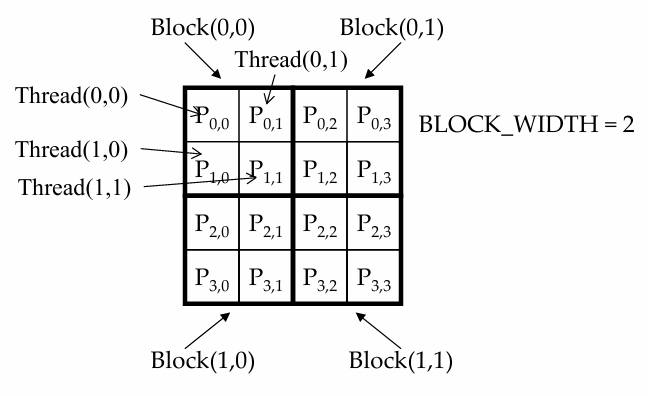
\includegraphics[width=0.6\textwidth]{figuresP/lesson_parallel_4_pag_36.png}
\end{center}
The code in App. \ref{app:matrix_example_cuda} is fairly complicated and using some time to read it and understand how it works can be a useful exercise. However our main point of interest is as follows.

Using the GeForce MX330, I executed the multiplication of 2 1024x1024 matrices with a grid of 16x16 blocks and got the following output. 
\begin{Verbatim}
[Output of > MatrixMultiplication_global 1024 1024 1024]
CUDA malloc A: no error
Copy A to device: no error
CUDA malloc B: no error
Copy B to device: no error
CUDA malloc C: no error
Run kernel: no error
Time: 36.52512 ms
Copy C off of device: no error
\end{Verbatim}
The execution lasted about 36 ms. You can try to write (or find online) a serial version of the same operation and you will find that it might take 30 s to 1 min to run with a normal CPU \footnote{The serial version of this code was run in class but I couldn't find it on the E-Learning platform of the course. However there are thousands of C programs for matrix multiplication published online that you can use as proof.}. Here the speed up is massive, about $10^4$. This is the most classic example of a \textbf{computation bound problem}: the latency of the CPU execution is due to the enormous amount of operations needed to complete the task, so using the GPU has given us an enormous boost.

We might already be happy with that, but it is possible to do better. For the multiplication of 2 NxN matrices we need N multiplications and N sums for each of the N elements in the result, for a total of 2N$^2$ FLOPs. However, once our matrices have been copied on the global memory of the device, it is necessary to access such memory 2N times for each element in order to retrieve the row and the column and compute the dot product. In other words, we also need 2N$^2$ memory accesses and our ratio "computation-to-memory access" is exactly 1. Let's consider this numerical example:
\begin{itemize}
    \item[-] Assume 100x100 matrices with single precision floating point elements (4 bytes).
    \item[-] In the GeForce MX330 the memory bandwidth (the amount of data that can be transferred from the global memory to the processor) is 56 GB/s.
    \item[-] How many operands (numbers to sum) per second can we load? \\ $56 \ \text{GB} / (2\text{N} \ \cdot \ 4 \ \text{bytes})=7\cdot10^9 \quad \Rightarrow$ \\
    We can load 7 billion operands per second.
    \item[-] Having a ratio "computation-to-memory access" of 1, that means that we can only execute 7 GFLOPS, which is very far from the 1.22 TFLOPS potential of the device!
\end{itemize}
In other words, our GPU could execute much more operations per second but it is constrained by the small memory bandwidth which slows everything down. The next step will be to escape (or at least limit) this memory access bottleneck.

That is exactly what the code \underline{MatrixMultiplication\_local.cu} in App. \ref{app:matrix_example_cuda} does. This is a very complicated example and we won't analyse it line by line, we will just explain the general principle behind it. 

As said, the global memory is a piece of hardware that is separated from the actual processor, but every multiprocessor also has an on-chip memory: the shared memory. Every thread run on the multiprocessor can write on and read the shared memory, and accessing it is orders of magnitude faster than the global one due to its physical vicinity to the cores. On the counter, it can contain only kilobytes or a few megabytes (for more modern devices) of information. That means that if we wanted to exploit the shared memory for our computations, there would not be enough space to copy all the matrices inside it. The trick is then to copy only a part of the data in the shared memory and then keep it there until all the operations that include it are completed. How do we apply that to matrices?

Take a look at the following figure that shows the multiplication $N \times M=P$. It becomes clear that once the line $M_{0,i}$ is copied in the shared memory, it can be rapidly used by all the threads that compute the elements in the line $P_{0,i}$, limiting the accessing to the global one.

\begin{center}
    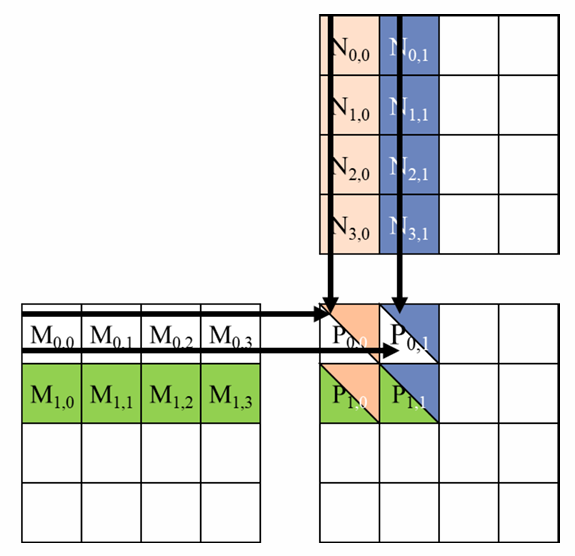
\includegraphics[width=0.35\textwidth]{figuresP/lesson_parallel_4_pag_37.png}
\end{center}

\begin{figure}[htbp]
    \begin{minipage}[c]{0.55\textwidth}
    Here is is the workflow applied in the complete code in App. \ref{app:matrix_example_cuda}:
    \begin{enumerate}
        \item Identify a “tile” of global memory contents that are accessed by multiple threads (e.g. a line of the M matrix);
        \item Load the tile from global memory into on-chip memory;
        \item Use barrier synchronization to make sure that all threads are ready to start the current execution phase (\texttt{\_\_syncthreads()});
        \item Have multiple threads access their data from the on-chip memory (and copy what's needed from the global one);
        \item Use barrier synchronization to make sure that all threads have completed the current phase;
        \item Move on to the next tile.
    \end{enumerate}
    \end{minipage}\hfill 
    \begin{minipage}[c]{0.4\textwidth}
        \centering
        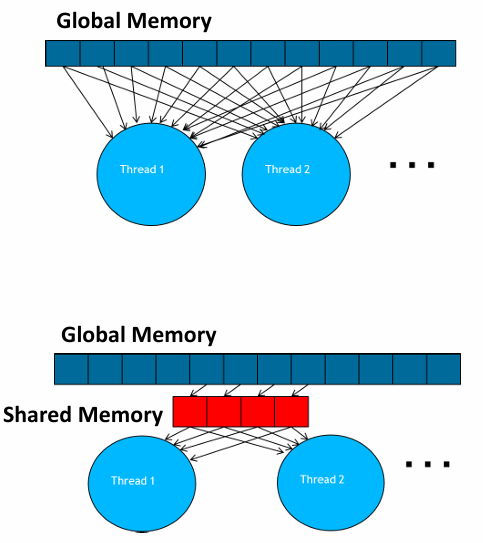
\includegraphics[width=\textwidth]{figuresP/lesson_parallel_4_pag_39.png}
    \end{minipage}
\end{figure} 
With this kind of implementation, the execution time was reduced to about 16 ms (more complex problems can experience much higher speed ups).

\hrulefill

\subsection{Note: Memory coalescing}

Another important concept that can be used for parallel programming is \textbf{memory coalescing}. We will not be implementing in with a practical example, but it is useful to know what it is.

In reality, both the global and shared memory (and even the RAM) are organized in groups called \textbf{bursts}: each address space is partitioned into burst sections and whenever a location is accessed, all other locations in the same section are also delivered to the processor, whether you like it or not. In practice, we have at least a 4GB address space, with burst section sizes of 128-bytes or more. If all accessed locations fall into the same burst section, only one RAM request will be made, and the access is said to be fully coalesced. When the accessed locations spread across burst section boundaries, coalescing fails. This means that in GPU computing it is useful (if possible) to organize our data in such a way that threads inside the same block will act on the same burst, in order to limit the number of memory accesses using coalescence. Otherwise some of the bytes transferred will not be used during the execution. The following figure shows a simple situation of a memory space organized in 4 burst of 4 bites and an example of coalesced memory load and un-coalesced memory load. 

\begin{center}
    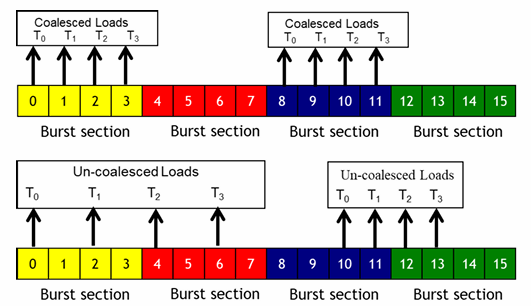
\includegraphics[width=0.5\textwidth]{figuresP/lesson_parallel_4_pag_46.png}
\end{center}

As a practical example, consider a standard matrix multiplication $A \times B = C$. As shown in the following figure, memory accesses to matrix B can easily be mapped sequentially along the rows ($B_{0,0}, B_{0,1}, \dots$), perfectly aligning with the contiguous burst sections and resulting in coalesced loads (top). Conversely, threads accessing matrix A must read down the columns ($A_{0,0}, A_{1,0}, \dots$). Because these values are scattered across different rows, each thread is forced to fetch data from an entirely different burst section, leading to un-coalesced access (bottom). A standard solution to speed up execution is to transpose the un-coalesced matrix (in this case, matrix A) prior to the operation. By reorganizing the data in memory, we allow the GPU to fetch the data in single and fully coalesced bursts.

\begin{center}
    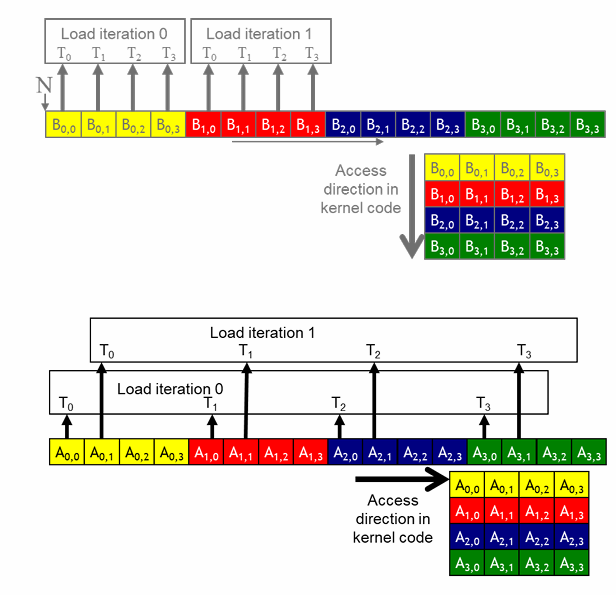
\includegraphics[width=0.5\textwidth]{figuresP/lesson_parallel_4_pag_47.png}
\end{center}

\begin{comment}
\subsection{HelloWorld}
HelloWorld example. Try to change the kernel launch parameters. Compile with \texttt{nvcc HelloWorld.cu -o HelloWorld -arch=compute\_35}.

\input{pygments/figuresP/lesson_parallel_4_pag_31.png}

\subsection{Vector Sum (Serial)}
We want to sum two vectors of 1048576 elements each. First we will try to write a "serial" version of the code. Due to the presence of cuda functions to measure the time, this code must be compiled with \texttt{nvcc}. Time: 4.4 ms (on GTX 650).

\input{pygments/figuresP/lesson_parallel_4_pag_32.png}

\subsection{Vector Sum (parallel)}
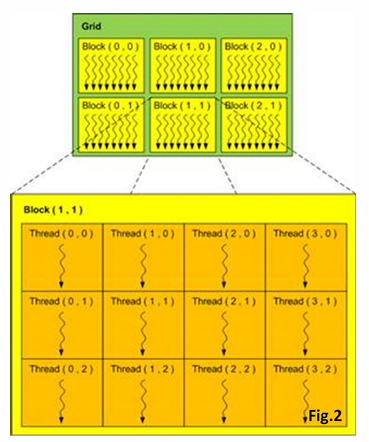
\includegraphics[width=0.6\textwidth]{figuresP/lesson_parallel_4_pag_33.png}

Let's try to parallelize, by using several blocks. Remember to copy data from host to device and results back. The results is not what we expect. Why? Time: 17.3 ms !!!

\input{pygments/figuresP/lesson_parallel_4_pag_33.png}

\subsection{Vector Sum (parallel): $2^\circ$ attempt}
Then let's try to use one single block and N Threads. Time = 0.01 ms, SpeedUp = 370. Uhmmmmmmmmmmmm. A reasonable speedup is around 100 or less. Try to print something: the results, the error code. Try to have a look to the maximum size of threads per block.

\input{pygments/figuresP/lesson_parallel_4_pag_34.png}

\subsection{Vector Sum (parallel): final attempt}
\includegraphics[width=0.6\textwidth]{figuresP/lesson_parallel_4_pag_35.png}

Use both threads and blocks. The total number of threads must be equal to the number of elements in the vectors. Define an "index" by using the block/thread identifier. The kernel must be adapted to this structure. Time = 0.48 ms (without errors).

\input{pygments/figuresP/lesson_parallel_4_pag_35.png}

\subsection{Matrix Multiplication}
Assume you want to multiply two large matrices. Use a 2D structure of threads and blocks. Each thread computes one element of the matrix. Use the blocks to subdivide the matrix in sub-blocks.

\input{pygments/figuresP/lesson_parallel_4_pag_36.png}

\subsection{Limitations to computing power}
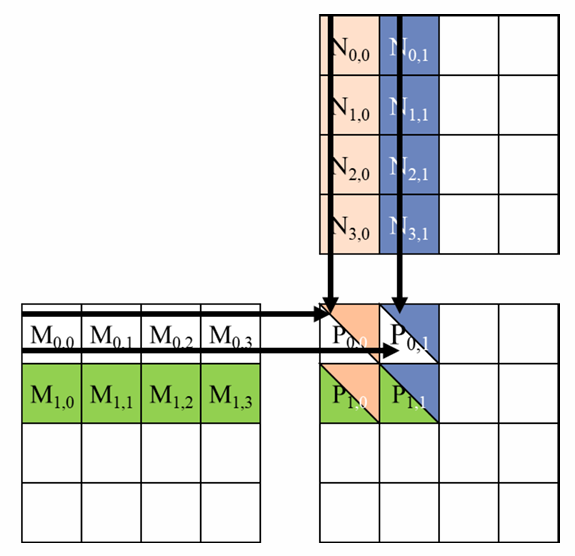
\includegraphics[width=0.6\textwidth]{figuresP/lesson_parallel_4_pag_37.png}

A lot of accesses to memory are required: for each element computed we need 2N global memory accesses, and 2N operations (N multiplications and N sums). The compute-to-global-memory-access ratio is 1:1.
In the K20 the memory bandwidth is 200 GB/s. Assuming $100\times100$ matrices, how many operands per second can we load? $200 \text{ GB} / (2N * 4\text{ bytes}) = 25 \text{ Goperands/s}$. Since the ratio is limited to 1, this means that the computing throughput is 25 GFlops, which is very far from the 3.5 TFlops capability of the board!

\subsection{Shared Memory}
\includegraphics[width=0.6\textwidth]{figuresP/lesson_parallel_4_pag_38.png}

Shared memory is a special type of memory whose contents are explicitly defined and used in the kernel source code. There is one in each SM, and it is accessed at much higher speed (in both latency and throughput) than global memory. The scope of access and sharing is restricted to thread blocks. Its lifetime corresponds to the thread block: contents will disappear after the corresponding thread block finishes execution. It is accessed by memory load/store instructions and acts as a form of scratchpad memory in computer architecture.

\begin{table}[H]
\centering
\begin{tabular}{|l|l|l|l|}
\hline
\textbf{Variable declaration} & \textbf{Memory} & \textbf{Scope} & \textbf{Lifetime} \\ \hline
\texttt{int LocalVar;} & register & thread & thread \\ \hline
\texttt{\_\_device\_\_ \_\_shared\_\_ int SharedVar;} & shared & block & block \\ \hline
\texttt{\_\_device\_\_ int GlobalVar;} & global & grid & application \\ \hline
\texttt{\_\_device\_\_ \_\_constant\_\_ int ConstantVar;} & constant & grid & application \\ \hline
\end{tabular}
\end{table}

\subsection{Shared memory for Matrix Multiplication}
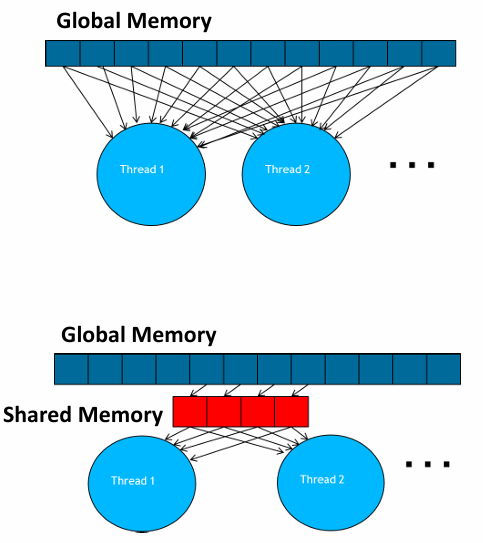
\includegraphics[width=0.6\textwidth]{figuresP/lesson_parallel_4_pag_39.png}

Identify a "tile" of global memory contents that are accessed by multiple threads. Load the tile from global memory into on-chip shared memory. Use barrier synchronization to make sure that all threads are ready to start the phase. Have the multiple threads access their data from the on-chip memory. Use barrier synchronization again to ensure that all threads have completed the current phase before moving on to the next tile.

\subsection{Shared memory: phase 0 load for block (0,0)}
During Phase 0 load, threads load tiles from matrices M and N into shared memory. For example, $thread_{0,0}$ loads $M_{0,0}$ and $N_{0,0}$.

\subsection{Shared memory: phase 0 use block (0,0)}
During Phase 0 use, threads compute partial products using the shared memory tiles. For example, $PValue_{0,0}$ accumulates $Mds_{0,0} * Nds_{0,0} + Mds_{0,1} * Nds_{1,0}$.

\subsection{Execution phases}
Threads execute loads and mathematical operations simultaneously in phases.
\textbf{Phase 0}:
$thread_{0,0}$ loads $M_{0,0}$ into $Mds_{0,0}$ and $N_{0,0}$ into $Nds_{0,0}$. It then computes $PValue_{0,0} += Mds_{0,0} * Nds_{0,0} + Mds_{0,1} * Nds_{1,0}$.
\textbf{Phase 1}:
$thread_{0,0}$ loads $M_{0,2}$ and $N_{2,0}$. It computes the next partial sum for $PValue_{0,0}$. This continues across all threads ($thread_{0,1}$, $thread_{1,0}$, $thread_{1,1}$) through time.

\subsection{Synchronization}
Synchronize all threads in a block using \texttt{\_\_syncthreads()}. All threads in the same block must reach the \texttt{\_\_syncthreads()} before any of them can move on. This is best used to coordinate phased execution in tiled algorithms, ensuring that all elements of a tile are loaded at the beginning of a phase, and that all elements of a tile are consumed at the end of a phase.

\subsection{MatrixMultiplication code}
HOST and GPU implementation for matrix multiplication utilizing shared memory.

\input{pygments/figuresP/lesson_parallel_4_pag_44.png}
\input{pygments/figuresP/lesson_parallel_4_pag_45.png}

\subsection{Memory coalescing}
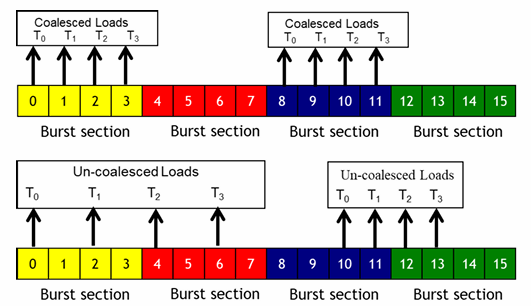
\includegraphics[width=0.6\textwidth]{figuresP/lesson_parallel_4_pag_46.png}

Each address space is partitioned into burst sections. Whenever a location is accessed, all other locations in the same section are also delivered to the processor. In practice, we have at least a 4GB address space, with burst section sizes of 128-bytes or more.
If all accessed locations fall into the same burst section, only one DRAM request will be made and the access is fully coalesced. When the accessed locations spread across burst section boundaries, coalescing fails. Multiple DRAM requests are made, and some of the bytes transferred are not used by the threads.

\subsection{Memory access in Matrix Multiplication}
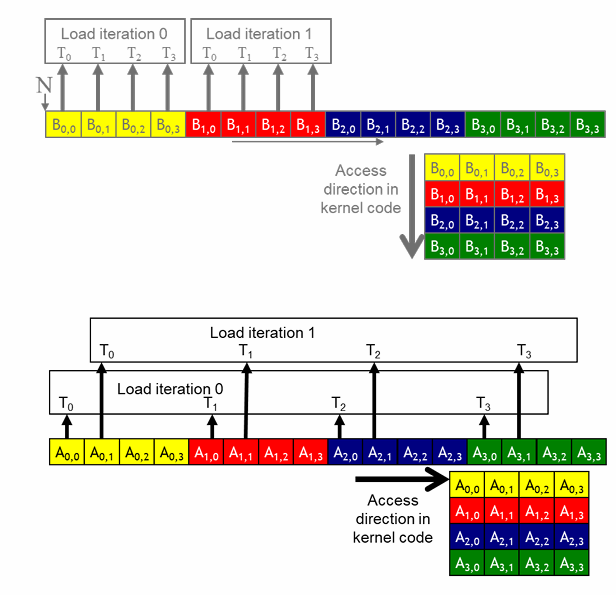
\includegraphics[width=0.6\textwidth]{figuresP/lesson_parallel_4_pag_47.png}

When loading rows/columns from matrices A and B: access to matrix B is coalesced because threads access contiguous memory locations. Access to matrix A is not coalesced because threads access data column-wise, spanning across different burst sections.

\subsection{For Hands-on next lecture}
We will use Colab (\url{https://colab.research.google.com}), requiring a Google account. It is based on Jupyter Notebook. Read the introduction on the first page. Colab allows you to use machines with GPU (and also TPU).

\subsection{Bibliography}
\textbf{Parallel programming:}
\begin{itemize}
    \item "The source book of parallel computing" (Dongarra et al.) - Morgan Kaufmann ed. (2003)
    \item "Introduction to parallel programming" (Grama-Gupta-Karypis-Kumar)
\end{itemize}
\textbf{Parallel processing in python:}
\begin{itemize}
    \item \url{https://docs.python.org/2/library/multiprocessing.html}
    \item \url{https://docs.python.org/3/library/threading.html}
\end{itemize}
\textbf{GPU online resources:}
\begin{itemize}
    \item \url{https://docs.nvidia.com/cuda/index.html}
    \item \url{https://docs.nvidia.com/pdf/CUDA_C_Programming_Guide.pdf}
    \item \url{https://docs.nvidia.com/pdf/CUDA_C_Best_Practices_Guide.pdf}
    \item \url{https://hgpu.org/} (collection of tutorials and articles)
\end{itemize}
\textbf{GPU books:}
\begin{itemize}
    \item "GPU Computing and Applications" (Yiju Cai) - Springer
    \item "Multicore and gpu programming: an integrated approach" (Barlas) - Morgan Kaufmann
    \item "Cuda by Example" (Sanders) - Addison-Wesley
    \item "Professional Cuda C programming" (Cheng et al.) - Wrox
\end{itemize}
\textbf{GPU in Python:}
\begin{itemize}
    \item \url{https://wish4book.com/education/5410-hands-on-gpu-computing-with-python.html}
    \item \url{https://documen.tician.de/pycuda/}
\end{itemize}

\subsection{Appendix: Purpose of this addendum}
The purpose of this addendum is to present some classic problems that can be addressed with GPU. The kernels proposed are deliberately incomplete (and sometimes also wrong). As an assignment, try to complete one or more of the proposed solutions to have a working kernel. Then try to include this kernel in a python code by using pyCUDA. Try to measure the timing of your implementation with respect to a simpler implementation or with respect to the serial version to show the speedup introduced by your work.

\subsection{Histograms}
\includegraphics[width=0.6\textwidth]{figuresP/lesson_parallel_4_pag_52.png}

Building histograms is a method for extracting features and patterns from large data sets. Typical applications include standard decryption methods, feature extraction for object recognition in images, search for decays in High Energy Physics, and correlating heavenly object movements in astrophysics. For each element in the data set, use the value to identify a "bin counter" to increment.

\subsection{Simple Histograms algorithm}
\includegraphics[width=0.6\textwidth]{figuresP/lesson_parallel_4_pag_53.png}

Partition the input into sections. Have each thread take a section of the input. Each thread iterates through its section. For each letter, increment the appropriate bin counter.

\subsection{Limits to "partitioning"}
\includegraphics[width=0.6\textwidth]{figuresP/lesson_parallel_4_pag_54.png}

Sectioned partitioning results in poor memory access efficiency. Adjacent threads do not access adjacent memory locations, therefore accesses are not coalesced and DRAM bandwidth is poorly utilized.

\subsection{Interleaved input access}
\includegraphics[width=0.6\textwidth]{figuresP/lesson_parallel_4_pag_55.png}

Change to interleaved partitioning. All threads process a contiguous section of elements. They all move to the next section and repeat. This way, memory accesses are coalesced. In this case, the logic partitioning is a little bit more complicated but the access to the memory is very efficient.

\subsection{Data races}
\includegraphics[width=0.6\textwidth]{figuresP/lesson_parallel_4_pag_56.png}

Interleaving solves the problem of access to the memory in input, but writing the histogram is still problematic. Different threads write at the same time in the same location in the output memory space. We have already seen the problem of data races in python multiprocessing. In GPU programming, it is not "natural" to use semaphores because the code is essentially SIMD.

\subsection{Atomic Operations}
A read-modify-write operation performed by a single hardware instruction on a memory location address. It reads the old value, calculates a new value, and writes the new value to the location. The hardware ensures that no other threads can perform another read-modify-write operation on the same location until the current atomic operation is complete. Any other threads attempting to access the same location will be held in a queue, forcing serial operations on that specific memory cell. Performed by calling intrinsic functions (e.g., atomic add, sub, inc, dec, min, max, exch, CAS).
For example, \texttt{atomicAdd(int* address, int val)} reads the 32-bit word \texttt{old} from the location pointed to by \texttt{address}, computes \texttt{old + val}, stores the result back, and returns \texttt{old+val}.

\subsection{Histograms kernel}
Assignment: Follow the example. Notice the stride and the use of \texttt{atomicAdd()}. Write the host code in Python and include the kernel by using \texttt{SourceModule} of pyCUDA. Define the "histogram" with the correct dimensions and plot it with matplotlib.

\input{pygments/figuresP/lesson_parallel_4_pag_58.png}

\subsection{Convolution}
The convolution is widely used in several fields (audio, image processing). It is the base of "stencil computing". A convolution is a filter that transforms signal or pixel values into more desirable values. Gaussian filters can be used to sharpen boundaries and edges of objects in images. Some filters smooth out the signal values so that one can see the big-picture trend.

\subsection{Computational definition of Convolution}
\includegraphics[width=0.6\textwidth]{figuresP/lesson_parallel_4_pag_60.png}

An array operation where each output data element is a weighted sum of a collection of neighboring input elements. The weights used are defined by an input mask array (convolution mask). The value pattern of the mask array elements defines the type of filtering done (e.g., Image blurring).

\subsection{1D Convolution example}
Example of calculating element $P[2]$ using inputs from $N$ and mask $M$: $P[2] = N[0]*M[0] + N[1]*M[1] + N[2]*M[2] + N[3]*M[3] + N[4]*M[4]$.

\subsection{1D convolution: boundaries}
\includegraphics[width=0.6\textwidth]{figuresP/lesson_parallel_4_pag_62.png}

Calculation of output elements near the boundaries (beginning and end) of the array need to deal with "ghost" elements. Different policies exist for this (e.g., using 0, replicates of boundary values, etc.).

\subsection{A simple stencil kernel}
\input{pygments/figuresP/lesson_parallel_4_pag_63.png}

\subsection{Calculation of adjacent output elements}
Calculation of adjacent output elements involves shared input elements. For example, $N[2]$ is used in the calculation of $P[0]$, $P[1]$, $P[2]$, $P[3]$, and $P[4]$ (assuming a 1D convolution mask of width 5). We can load all the input elements required by all threads in a block into the shared memory to reduce global memory accesses.

\subsection{Subdivide the input array in tiles}
Subdivide the input array in tiles. Each tile is $nP$ elements large, where $nP$ is the number of threads in a block. Cache data in shared memory. All the threads in a block will copy one element into the shared memory from the global memory. $2 * \text{radius}$ extra elements (where radius is the width of the halo around the $nP$ elements) are also included to handle boundaries.

\subsection{Shared memory stencil 1D}
\input{pygments/figuresP/lesson_parallel_4_pag_66.png}

\subsection{Parallel reduction}
\includegraphics[width=0.6\textwidth]{figuresP/lesson_parallel_4_pag_67.png}

A large class of algorithms on large data sets are based on the idea to reduce the amount of interesting information. Google and Hadoop MapReduce frameworks support this strategy. There is no required order for processing elements in a data set (associative and commutative operations like Max, Min, Sum, Product). You partition the data set into smaller chunks, have each thread process a chunk, and then use a reduction tree to summarize the results from each chunk into the final answer.

\subsection{Simple Parallel reduction tree}
In a simple parallelization, each operation is performed by a different task. For $N$ initial values, the tree performs $(N-1)$ operations in $\log(N)$ parallel steps. The average parallelization per step is $(N-1)/\log(N)$. For example, if $N=1000000$, we have on average 50000 parallel workers, but the peak requires 500000 parallel workers (in step 1), while the last step needs only one worker. This represents a very inefficient use of parallel resources, particularly for SIMD. It's a good idea to rethink the parallel structure to efficiently reuse the computing units.

\subsection{Parallel sum with shared memory}
\includegraphics[width=0.6\textwidth]{figuresP/lesson_parallel_4_pag_69.png}

Recursively halve the number of threads, adding two values per thread in each step. This takes $\log(n)$ steps for $n$ elements and requires $n/2$ threads. This assumes an in-place reduction using shared memory. The original vector is in device global memory; shared memory is used to hold a partial sum vector. Each step brings the partial sum closer to the total sum, which will ultimately be in element 0. Thread block size limits $n$ to be $\le 2048$. This greatly reduces global memory traffic.

\subsection{Additional assignment}
Try to write the GPU version of the assignment proposed in the processing in Python lecture. Measure the speedup with respect to multithreading and multiprocessing and produce a plot to compare the results.

\subsection{License}
\includegraphics[width=0.6\textwidth]{figuresP/lesson_parallel_4_pag_71.png}

Part of the material used for this presentation comes from the "GPU Teaching KIT" licensed by NVIDIA and University of Illinois, and has been used and modified according to Creative Commons attribution non-commercial 4.0.

\end{comment}
\section{Hands-on examples for parallel programming (2)}\label{sec:hands_on_cuda_2}

\subsection{PyCUDA Module and Numba}
As you might have suspected from the last sections, the world of GPUs is vast and complex, and C is not the easiest and most readable language to use for your everyday coding. Understanding CUDA, its standards and its mechanisms is mandatory, but fortunately, fellow Python users, there are some ways to make our lives a little easier. 

PyCUDA is a powerful module that lets you access NVIDIA's CUDA parallel computation API directly from Python. This means all standard CUDA features can be easily accessed through it. PyCUDA supports Just-In-Time (JIT) compilation of CUDA kernels written in C, while maintaining a very small overhead with respect to a pure C implementation for the GPU part.  Furthermore, it provides several additional quality-of-life features, such as translating native CUDA exceptions into standard Python exceptions. One of the main virtues of PyCUDA is that it allows us to use the \texttt{GPUArray} class to handle memory transfers smoothly. We will dive deeper into all of this in the following examples.

Alongside PyCUDA, we will also use Numba to compile universal functions (ufuncs) directly on the GPU.

Here are some useful references on these two modules:
\begin{itemize}
    \item[-] \url{https://pypi.org/project/pycuda/}
    \item[-] \url{https://documen.tician.de/pycuda/}
    \item[-] \url{http://numba.pydata.org/numba-doc/latest/cuda/index.html}
\end{itemize}

\textbf{Google Colab}, also known as \textit{Colaboratory}, is a free \textit{Jupyter} notebook environment running on the Google Cloud. It provides an accessible environment to write text and run Python 3 (and many other) code directly from your browser, with the notebooks being automatically stored in your Google Drive. One of its main advantages is the ability to run your code on cloud computers housing dedicated GPUs. Thanks to the underlying IPython library, it is also possible to execute shell commands---including compilers---directly on the cloud filesystem, as well as install and add new modules to your development environment. If you don't have a GPU to work with, you can start working on Colab (\url{http://colab.research.google.com}) to run your GPU-based programs.

For this section, we are going to use a Jupyter Notebook which you can find at the following link: \url{https://colab.research.google.com/drive/1C3bY-DKcyOp067Nti08JZ8cfnfz9YmCK?usp=sharing}. With respect to the corresponding notebook that you will surely find on the E-Learning page of the course, here some comments and notes have been added to make it more readable and clear. Try to run it on Colab or on your local PC.

Since I have to start a new page in order to input the Notebook in my LaTeX file, here is a photo of Dustin Brown executing a backhand volley against Rafael Nadal during the 2015 Wimbledon tournament. Brown went on to defeat Nadal in 4 sets with a flashy, fearless and dominant performance, with probably the best opening game in the history of tennis.

\begin{center}
    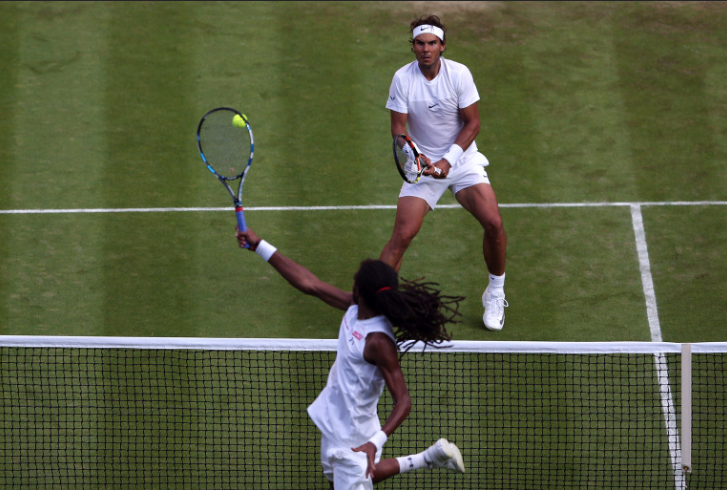
\includegraphics[width=0.3\textwidth]{figuresP/dustin_brown.png}
\end{center}

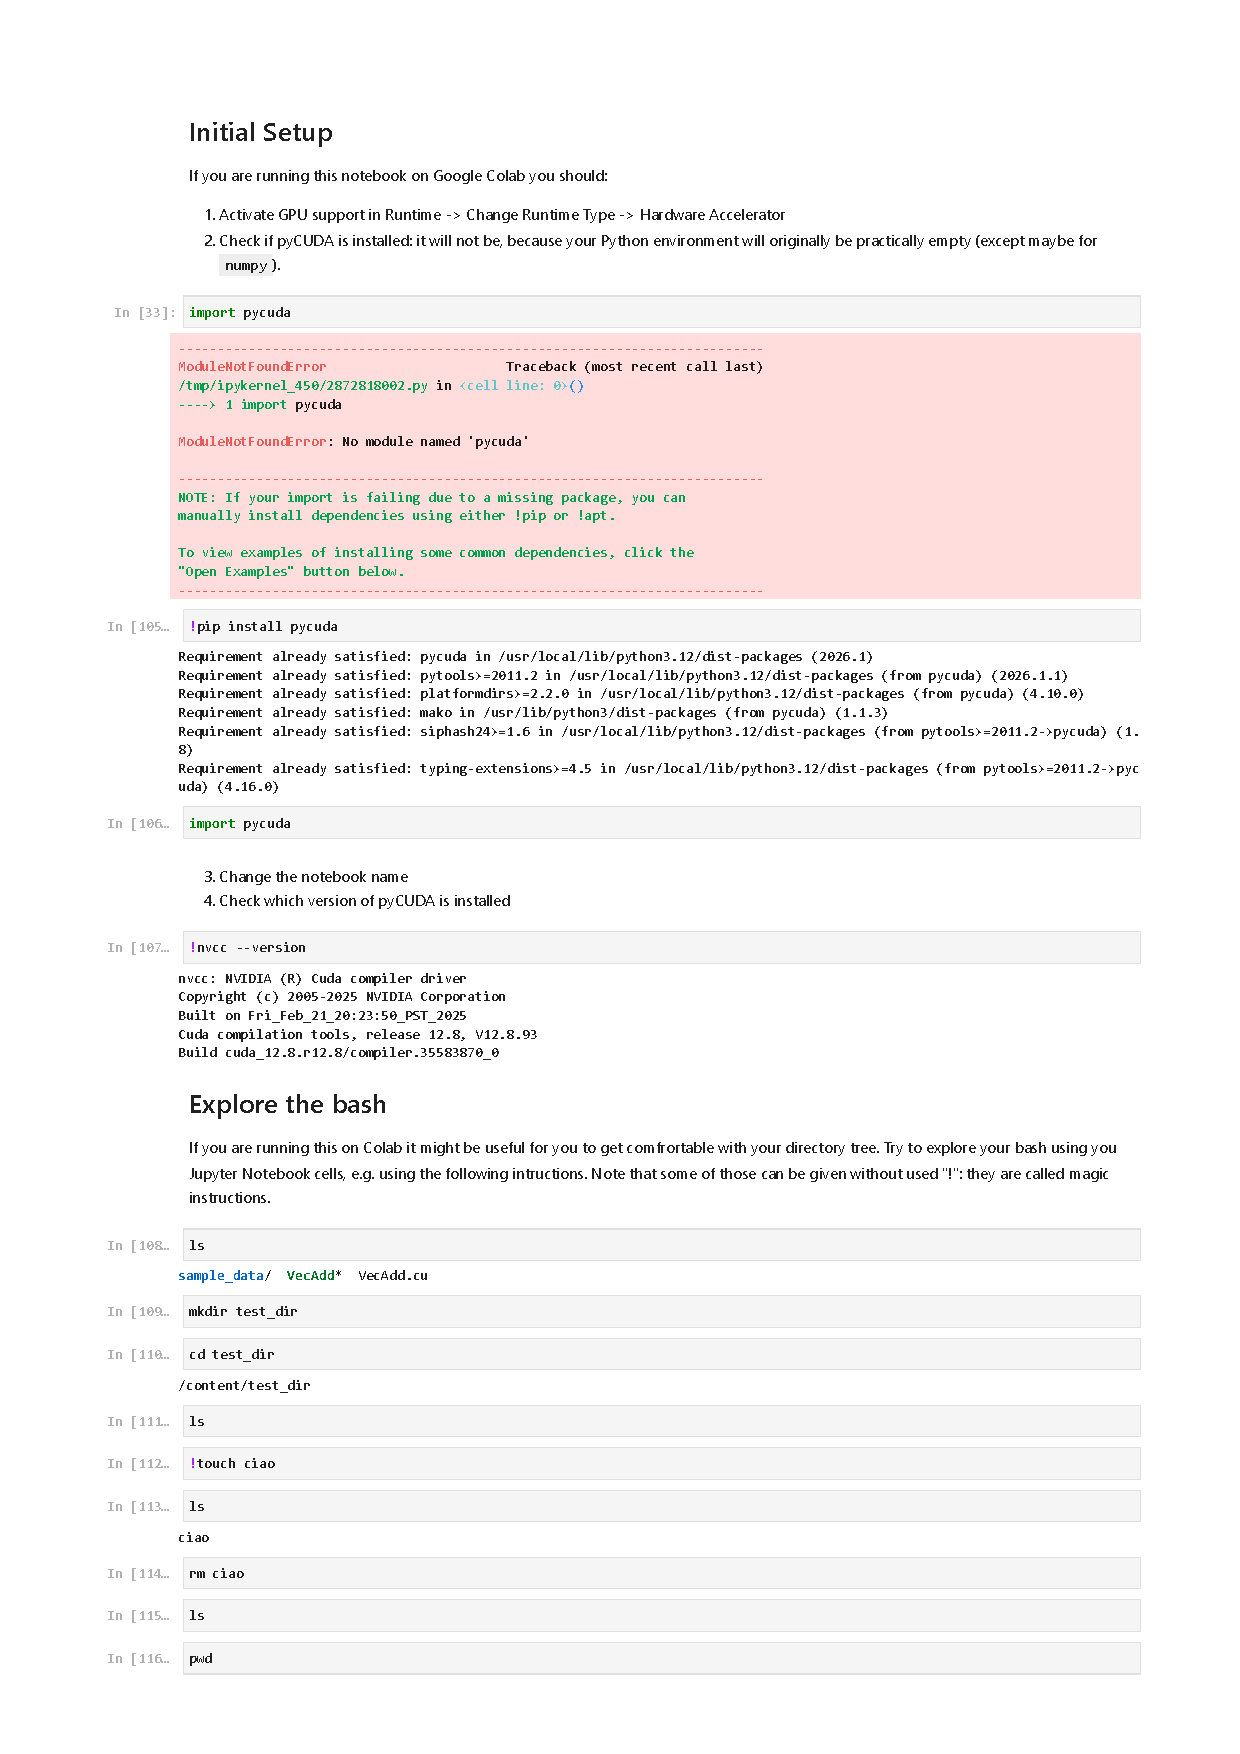
\includepdf[pages=-, pagecommand={\thispagestyle{plain}}]{lezioni/c_parallel5A_GPU.pdf}

\subsection{Bibliography}
\textbf{Parallel programming:}
\begin{itemize}
    \item[-] "The source book of parallel computing" (Dongarra et al.) - Morgan Kaufmann ed. (2003)
    \item[-] "Introduction to parallel programming" (Grama-Gupta-Karypis-Kumar)
\end{itemize}
\textbf{Parallel processing in Python:}
\begin{itemize}
    \item[-] \url{https://docs.python.org/2/library/multiprocessing.html}
    \item[-] \url{https://docs.python.org/3/library/threading.html}
\end{itemize}
\textbf{GPU online resources:}
\begin{itemize}
    \item[-] \url{https://docs.nvidia.com/cuda/index.html}
    \item[-] \url{https://docs.nvidia.com/pdf/CUDA_C_Programming_Guide.pdf}
    \item[-] \url{https://docs.nvidia.com/pdf/CUDA_C_Best_Practices_Guide.pdf}
    \item[-] \url{https://hgpu.org/} (collection of tutorials and articles)
\end{itemize}
\textbf{GPU books:}
\begin{itemize}
    \item[-] "GPU Computing and Applications" (Yiju Cai) - Springer
    \item[-] "Multicore and GPU programming: an integrated approach" (Barlas) - Morgan Kaufmann
    \item[-] "Cuda by Example" (Sanders) - Addison-Wesley
    \item[-] "Professional Cuda C programming" (Cheng et al.) - Wrox
\end{itemize}
\textbf{GPU in Python:}
\begin{itemize}
    \item[-] \url{https://wish4book.com/education/5410-hands-on-gpu-computing-with-python.html}
    \item[-] \url{https://documen.tician.de/pycuda/}
\end{itemize}
%\end{comment}

% -------------------------------------------------------------------
% PART III: Machine Learning (Basis)
% -------------------------------------------------------------------
\chapter[Introduction to Machine Learning]{Introduction to Machine Learning \\[0.5ex] \large \textit{(Prof.essa Retico, Prof. Di Bello, Prof. Rizzi)}}

%\begin{comment}
\section{Basics of Machine Learning}

\subsection{Some initial references}
Here are some resources that could help you for this next chapter:

\textbf{Books}:
\begin{itemize}
    \item \emph{Deep Learning Book} (Ian Goodfellow, Yoshua Bengio and Aaron Courville), \url{https://www.deeplearningbook.org/}
    \item \emph{The 100 pages ML book} (Andriy Burkov), \url{http://themlbook.com/wiki/doku.php}
    \item \emph{Deep Learning with Python} (Francois Chollet)
    \item \emph{The Elements of Statistical Learning} (Friedman, Tibshirani and Hastie)
\end{itemize}

\textbf{Online resources}:
\begin{itemize}
    \item Machine Learning Stanford Course: \url{https://cs229.stanford.edu/main_notes.pdf}
    \item Convolutional Neural Network for Visual Recognition, Stanford Course (also on YouTube): \url{https://cs231n.github.io/}
\end{itemize}

\textbf{Data Set}:
\begin{itemize}
    \item \url{https://www.cancerimagingarchive.net/}
    \item \url{https://www.kaggle.com/}
\end{itemize}


\subsection{Basic definitions and outline}

By \textbf{Artificial Intelligence (AI)}, we mean a set of techniques that rely on automatic learning by a machine to solve a complex and specific problem. 
\textbf{Machine Learning (ML)} is a vast field that includes many types of algorithms capable of learning to solve even very complex problems. 
In particular, \textbf{Deep learning (DL)} is machine learning made with \textbf{Deep Neural Networks (DNN)}, which we will learn to use in due time.

The basic idea is this: \textit{instead of producing rule-based algorithms we let the algorithm learn the rules}. Applications include for example autonomous driving, image and speech processing, agents able to play chess, play Go or drive cars, chatbots, anomaly detection (e.g. in credit card usage), and applications for research in various scientific fields (e.g. physics and medicine). For example, typical tasks include \textit{classification} (giving a discrete label to a certain type of data), \textit{segmentation} (assigning a class label to every fundamental unit of a data sample, such as a pixel in an image), \textit{regression} (predicting a continuous numerical output), \textit{super-resolution} (high-resolution image reconstruction from low-resolution images) and \textit{data generation} (creating new, synthetic data samples that resemble the original training distribution). 

%\includegraphics[width=0.8\textwidth]{lesson_ml_1_pag_4.png}

Here is a brief overview of the program we are going to follow in order to dive into the modern (and, in all fairness lucrative) world of machine learning:
\begin{enumerate}
    \item Introduction to basic concepts: 
    \begin{itemize}
        \item[-] Hypothesis function/Objective function
        \item[-] Training and inference
        \item[-] Learning paradigms (supervised, unsupervised and reinforcement) 
    \end{itemize}
    \item Supervised Learning:
    \begin{itemize}
        \item[-] Linear Regression
        \item[-] Logistic Regression (Cost function and optimization, Gradient Descent, Learning Rate).
    \end{itemize}
    \item Unsupervised learning: 
    \begin{itemize}
        \item[-] K-means algorithm
        \item[-] PCA
    \end{itemize} 
    \item Decision Tree.
    \item Capacity, underfitting, overfitting, bias-variance trade-off
    \item Regularization
    \item Data Management: 
    \begin{itemize}
        \item[-] Train/Validation/Test split
        \item[-] Cross-validation
        \item[-] Model selection
    \end{itemize} 
    \item Metrics
\end{enumerate}

\subsection{The hypothesis function and the 3 learning paradigms}
The goal of a ML algorithm is to approximate an unknown function (called hypothesis function $h(x)$ or often simply model) given some example data. If the output is continuous, we talk about \textbf{regression}; if the output is discrete, we talk about \textbf{classification}. In the figure below is a scheme that shows how a ML algorithm is built: we will dive deeper in all of its components.

\begin{center}
    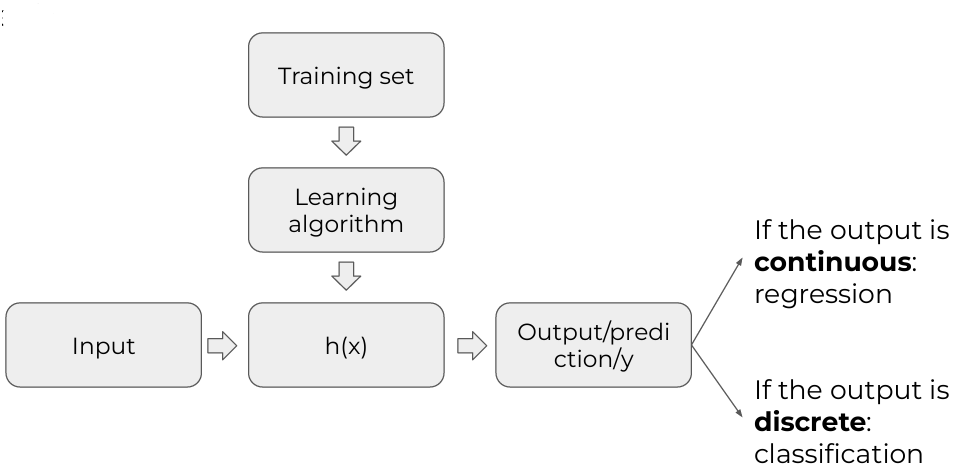
\includegraphics[width=0.8\textwidth]{figuresML/lesson_ml_1_pag_6.png}
\end{center}

We can distinguish two different phases in each ML algorithm:
\begin{itemize}
    \item[-] \textbf{Training phase} is the phase where the algorithm is allowed to change its parameters to learn how to approximate the function. We are going to call $\theta$ the parameters the model learns to solve the problem, i.e. to predict the correct output.
    \item[-] \textbf{Inference phase} is the test of a trained algorithm on unseen data. Of course, in this phase the algorithm cannot change its parameters.
\end{itemize}

There are thousands of learning algorithms, but each of them implements one of 3 types of \textbf{learning paradigms}:
\begin{itemize}
    \item[-] \textbf{Supervised}: Many inputs or \textbf{features} ($x$) associated with their \textbf{targets} ($y$, often referred to as \textit{labels} or \textbf{ground truth}) are given to the algorithm. We call "example" each $(x^{(i)},y^{(i)})$ couple, since $y$ represents the expected output given the input $x$ of the function $h$ we are trying to approximate. The algorithm has to find the underlying connections between data that solve a specified task, i.e. to find the best parameters for $h$.
    \item[-] \textbf{Unsupervised}: Many training samples ($x$) without a specific label are used to train the algorithm. The algorithm should learn to discover patterns, groupings, and relationships within the data without explicit guidance or prior knowledge of the desired outcomes. This paradigm can be much more difficult to implement with respect to the supervised one, since in this case we are forced to make stronger assumptions for weaker guarantees. The upside is that we are probably going to get much more information out of our dataset, since it can be used even if we do not have the "answers" to feed to the agent during training.
    \item[-] \textbf{Reinforcement}: In the reinforcement learning framework, we provide our algorithms only a \textit{reward function}, which indicates to the learning agent when it is doing well, and/or a penalty when it is doing poorly. This is the learning paradigm used to teach an algorithm to play chess or GO.
\end{itemize}

We will mainly focus our attention on supervised and unsupervised algorithms.

\subsection{Supervised learning: Gradient descent methods for regression}
We are going to go through a simple case of supervised learning in order to understand its basic principles. 

Let $d$ be the number of features and $n$ the number of training examples, so that our training set is a set of examples $(x, y)$. 
Assume that our hypothesis function is that input and output (continuous) are linearly related:
\begin{equation}
h(x) = \sum_{j=0}^{d} \theta_{j} x_{j}
\end{equation}
As said, training means finding the parameters $\theta$ that better fit the data $x$. 

We want to choose $\theta$ such that $h(x) \approx y$ for the training examples. To achieve this, we need to define a \textbf{cost function} (or loss function) which basically tells us how far our approximation is from the correct answer. In this case, we choose the \textit{mean squared error}:
\begin{equation}
J(\theta) = \frac{1}{2n}\sum_{i=1}^{n}(h_{\theta}(x^{(i)}) - y^{(i)})^{2}
\end{equation}
This kind of problem should look familiar: we are just implementing the ordinary \textit{least squares method} for \textit{linear regression}. However, the choice of the loss function depends on the kind of the problem. For instance...
\begin{itemize}
    \item[-] ... if we have a classification task we can use the so called \textit{Binary Cross Entropy}: 
    \begin{equation*}
        D_{BCE}(y,\hat{y}) = -\frac{1}{N}\sum_{i=1}^{N}[y_{i}\log(\hat{y}_{i}) + (1-y_{i})\log(1-\hat{y}_{i})]
    \end{equation*}
    \item[-] ... if we have a segmentation task we can use the so called \textit{Dice Loss}: 
    \begin{equation*}
        DSC_{loss} = 1 - 2\frac{|X \cap Y|}{|X \cup Y|}
    \end{equation*}
\end{itemize}
Whatever loss function we are using the goal is always the same: we need to \textbf{minimize it}.

We start with random parameters ($\theta_{random}$) and keep changing $\theta$ to reduce the cost function $J(\theta)$. Considering a fixed dataset, implementing a \textbf{Gradient Descent (GD) algorithm} means updating the parameters following this rule:
\begin{equation}
\theta_{j} := \theta_{j} - \alpha \frac{\partial J(\theta)}{\partial\theta_{j}} \quad \text{for } j=0,...,d
\end{equation}
This formula means that we take the old value of the parameter $\theta_j$ and modify it towards the direction where the gradient of the error function is steeper. With the help of the following figure you can already note a fundamental problem: depending on the initialization parameters we could reach different minimums every time. 

\begin{center}
    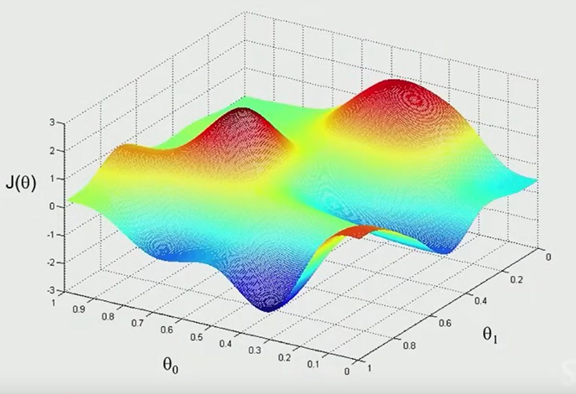
\includegraphics[width=0.6\textwidth]{figuresML/lesson_ml_1_pag_17.png}
\end{center}

The parameter $\alpha$ is called \textbf{Learning Rate (LR)} and it is actually a hyperparameter: parameters ($\theta$) change during training, while hyperparameters include all the choices made by the programmer that cannot be learnt by the algorithm. The "length of the step" we make in one iteration is given by the value of the learning rate.
Here is a pivotal fact: \textbf{the wrongful choice of the learning rate can break your learning algorithm}. Take a look at the following figure. Note that:
\begin{itemize}
    \item[-] if you choose a low value for $\alpha$, the process will be slow and you will need a lot of computational power in order to reach a minimum;
    \item[-] if you choose a high value for $\alpha$, you might not reach the minimum at all given the fact that your "steps" might be so long that your algorithm might start to oscillate, just as in this figure.
\end{itemize}
One of the best ways to decide the learning rate is an \textit{adaptive way: while the loss is approaching the minimum, we decrease the learning rate!}

\begin{center}
    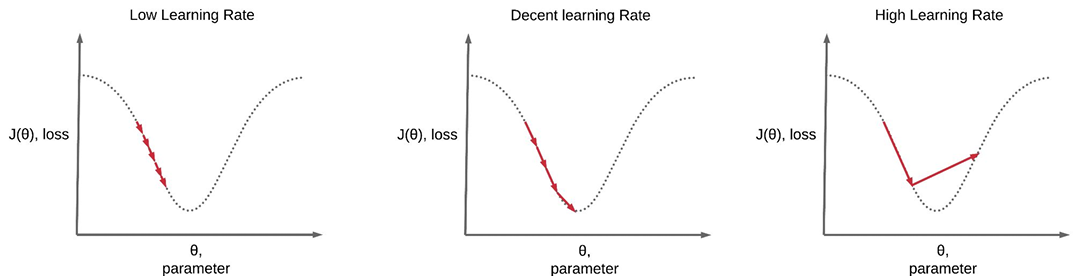
\includegraphics[width=0.69\textwidth]{figuresML/lesson_ml_1_pag_20.png} $\ \rightarrow \ $
    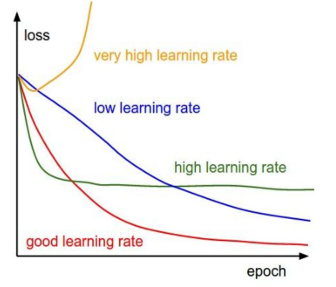
\includegraphics[width=0.23\textwidth]{figuresML/lesson_ml_1_pag_21.png}
\end{center}

If we go back to our example for a second, we see that we can compute the partial derivative of $J$ with respect to $\theta_j$ in the case of linear regression and squared error:
\begin{equation}
\theta_{j} := \theta_{j} + \alpha\frac{1}{n}\sum_{i=1}^{n}(y^{(i)} - h_{\theta}(x^{(i)}))x_{j}^{(i)}
\end{equation}

The method underlined in the last few paragraphs looks at every example in the entire training set on every step and it is called \textbf{Batch Gradient Descent (BGD)} or simply \textbf{Gradient Descent (BGD)}. There is an alternative called the \textbf{Stochastic Gradient Descent (SGD)} which, instead of using all the training examples, uses only one of them and makes the upgrade. The SGD has many drawbacks such as:
\begin{itemize}
    \item[-] it is prone to converge to local optima;
    \item[-] may get trapped in saddle points in certain cases;
    \item[-] it makes it difficult to choose a suitable learning rate;
    \item[-] all parameters use the same learning rate.
\end{itemize}
The most used method nowadays (practically the default if possible) is the so called \textbf{Mini-batch SGD}: instead of using all the input data or only one, we use a bunch of them and then we average the gradients.

\subsection{Supervised learning: Binary classification in a probabilistic approach}

In a \textit{binary classification} task, the goal is to categorize data into one of two mutually exclusive classes. By convention, these classes are mathematically represented as $y \in \{0, 1\}$. For example you might want to determine whether an email is spam ($1$) or not ($0$), or whether a medical tumour is malignant ($1$) or benign ($0$).

You might have thought to apply our previous linear regression model, $h(x) = \theta^{T}x$, and simply set a threshold to separate the classes. However, this approach is fundamentally flawed since the output of a linear combination can range from $-\infty$ to $+\infty$, whereas we want to interpret our hypothesis as the \textit{probability} that an example belongs to the positive class. By definition, probabilities must be strictly bounded in the $[0, 1]$ interval. To achieve this, we need to change our hypothesis function to the \textbf{sigmoid (or logistic) function}:
\begin{equation}
    h_{\theta}(x) = g(\theta^{T}x) = \frac{1}{1+e^{-\theta^{T}x}}
\end{equation}
The derivative of the sigmoid is nice because it is equal to: $g^{\prime}(z) = g(z)(1-g(z))$.

\begin{center}
    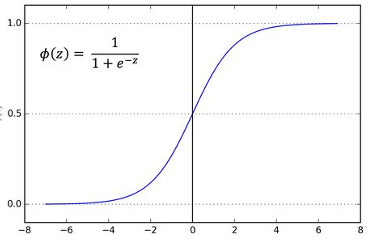
\includegraphics[width=0.4\textwidth]{figuresML/lesson_ml_1_pag_24.png}
\end{center}

Let's assume that $p(y=1|x;\theta) = h_{\theta}(x)$ and $p(y=0|x;\theta) = 1-h_{\theta}(x)$. We can write this more compactly as: 
\begin{equation}
p(y|x;\theta) = (h_{\theta}(x))^{y}(1-h_{\theta}(x))^{1-y}
\end{equation}
Assuming that the $n$ training examples were generated independently, we can write the so called \textbf{Likelihood} function:
\begin{equation}
L(\theta) = p(\vec{y}|x;\theta) = \prod_{i=1}^{n} (h_{\theta}(x^{(i)}))^{y^{(i)}} (1-h_{\theta}(x^{(i)}))^{1-y^{(i)}}
\end{equation}
The likelihood is the probability of observing the data conditioned by the parameters $\theta$. This is just another way to proceed: instead of defining a loss function to minimize (which you can also do), here we just use a likelihood that of course needs to be maximized.

For computational efficiency we can maximize a strictly increasing function of the likelihood, like its $\log$:
\begin{equation}
l(\theta) = \log L(\theta) = \sum_{i=1}^{n} y^{(i)}\log h(x^{(i)}) + (1-y^{(i)})\log(1-h(x^{(i)}))
\end{equation}
Now, we have to maximize it via gradient ascent just like before:
\begin{equation*}
\dfrac{\partial l}{\partial \theta_j}= ... = \sum_{i=1}^{n}(y^{(i)}-h_\theta (x^{(i)}))x^{(i)}_j \quad \Rightarrow
\end{equation*}
\begin{equation}
\theta_{j} := \theta_{j} + \alpha\sum_{i=1}^{n}(y^{(i)} - h_{\theta}(x^{(i)}))x_{j}^{(i)}
\end{equation}

\subsection{Unsupervised learning: K-means}

In this scenario, we do not have any label, we see only our inputs/points. We assume that there exists a latent or hidden structure inside the input data. The question is: can I recover it? 
The kind of problems we can solve with this approach are:
\begin{enumerate}
    \item Classification of "common'' patterns (clustering)
    \item Dimensionality reduction, compression
    \item Prediction of missing inputs
    \item Anomaly detection
\end{enumerate}

\begin{figure}[H]
    \begin{minipage}[c]{0.55\textwidth}
    Let's suppose we want to perform a clustering of input data $x^{(1)},...,x^{(n)} \in \mathbb{R}^{d}$ and $k$ is the number of clusters. We must find an assignment of points to clusters $C^{(i)}=j$ assuming that each point belongs only to one cluster. Note that one of the main problems with this approach could be defining the number $k$ itself. One way to do that is using the so called \textbf{K-means} algorithm:
    \begin{enumerate}
        \item Randomly initialize point centers $\mu^{(1)}, \dots, \mu^{(k)}$.
        \item Define a distance and assign each point to a cluster following the rule \\ $C^{(i)} = \text{argmin}_{j} (||\mu^{(j)} - x^{(i)}||)$.
        \item Compute new cluster centers as the mean of the positions of the points of the clusters.
        \item Repeat until convergence, that is when centers points do not change between different iterations.
\end{enumerate}
    \end{minipage}\hfill 
    \begin{minipage}[c]{0.4\textwidth}
        \centering
        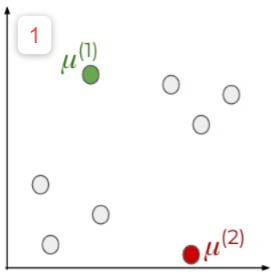
\includegraphics[width=0.48\linewidth]{figuresML/lesson_ml_1_pag_30.png}\hfill
        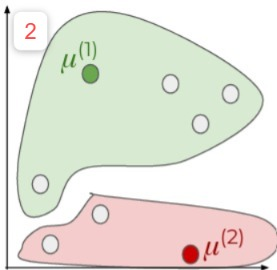
\includegraphics[width=0.48\linewidth]{figuresML/lesson_ml_1_pag_31.png} \\[.25cm] 
        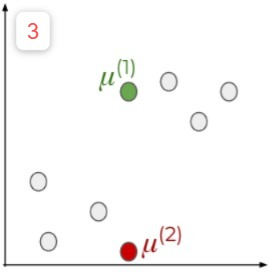
\includegraphics[width=0.48\linewidth]{figuresML/lesson_ml_1_pag_32.png}\hfill
        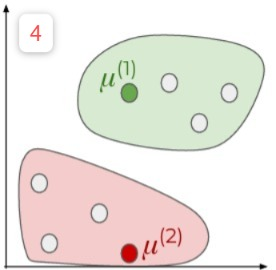
\includegraphics[width=0.48\linewidth]{figuresML/lesson_ml_1_pag_33.png}
    \end{minipage}
\end{figure} 

\subsection{Unsupervised learning: Principal Component Analysis (PCA)}
The so called \textbf{Principal Component Analysis (PCA)} algorithm is used for dimensionality reduction (which is pivotal since it may happen that you have more features than samples in your data) to simplify complex datasets. PCA aims to find new variables (called \textbf{principal components}) that are linear combinations of the original variables. These new variables are orthogonal (uncorrelated) and capture the maximum possible variance in the data.

Here's how PCA works:
\begin{enumerate}
    \item \textit{Data Standardization}: each variable is centered (by subtracting the mean) and scaled (by dividing for the standard deviation).
    \item \textit{Covariance Matrix Computation}: Compute the covariance matrix which captures how the variables vary together: $\Sigma = \frac{1}{1-N} X^{T}X$.
    \item \textit{Eigenvalue and Eigenvector Computation}: The eigenvectors of the covariance matrix define the directions of the principal components, while the eigenvalues indicate how much variance is explained by each of them.
    \item \textit{Selection of Principal Components}: The first $k$ components that explain the most variance are selected, as represented in the following figure. $k$ must be chosen wisely: if $k$ is too low we might not be able to solve our task, if it is too high you might end up using a lot of computational power. 
    \item \textit{Data Projection}: the original data is projected onto the space defined by the selected components, resulting in a dataset with fewer dimensions.
\end{enumerate}

\begin{center}
    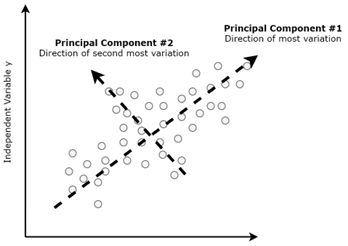
\includegraphics[width=0.35\textwidth]{figuresML/lesson_ml_1_pag_34.png}
\end{center}

\subsection{Supervised learning: $k$-Nearest neighbors}

The \textbf{$k$-Nearest Neighbors (kNN)} algorithm is a very powerful, instance-based method used for both classification and regression tasks. Unlike other algorithms that learn an explicit internal model during the training phase, kNN is considered a "lazy learner." Its core mechanism involves evaluating a new, unseen sample by looking at the data points in the training dataset that are \textit{close} to the sample itself in the feature space.

Here is how the algorithm generally operates:
\begin{itemize}
    \item[-] We choose a parameter \textbf{$k$}, which represents the number of neighbors.
    \item[-] We compute the distance between the new sample and all the points in the training set.
    \item[-] We look at the $k$ closest samples.
    \item[-] The final prediction is then made based on these neighbors (e.g., by a majority vote for classification, or by averaging the targets for regression).
\end{itemize}

Multiple neighbors ($k > 1$) can be used for a more stable evaluation, as it makes the algorithm's predictions less sensitive to noise or outliers in the training data. However, this approach comes with a significant drawback: on large datasets, it could be a major computational and memory problem to keep all training points available and calculate distances against them during the evaluation phase.

While they both rely on spatial distance, kNN and K-means serve entirely different purposes and belong to different learning paradigms:
\begin{itemize}
    \item[-] \textbf{kNN} is a \textit{supervised learning} algorithm. It relies on a completely labeled training dataset to predict the specific class or continuous target of a new, individual data point.
    \item[-] \textbf{K-means}, as discussed in the previous sections, is an \textit{unsupervised learning} algorithm. It operates on completely unlabeled data with the goal of discovering hidden structures, partitioning the entire dataset into $K$ distinct clusters.
\end{itemize}

\subsection{Another way to classify data: Decision Trees}
A \textbf{decision tree} is a predictive model, where leaves represent class labels and branches represent conjunctions of features that lead to those class labels. It is very hard to solve some problems with a linear model. Take a look at the example below which contains 2 classes (negative and positive) of points in a 2 dimensional feature space ($x_1 \in [0,12]$, $x_2 \in [-90, 90]$): it is clear that linear regression and clustering will not work for our classification task.

\begin{center}
    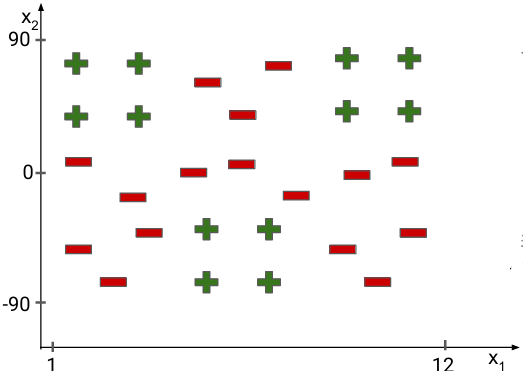
\includegraphics[width=0.35\textwidth]{figuresML/lesson_ml_1_pag_36.png}
\end{center}

Now we should try to isolate a cluster of negatives (a \textbf{leaf}) by imposing some conditions on $x_1$ and $x_2$ (\textbf{nodes}). The "tree" structure appears as a sequence of choices (which define the \textbf{branches}) is made until convergence is reached, as shown below. 

\begin{center}
    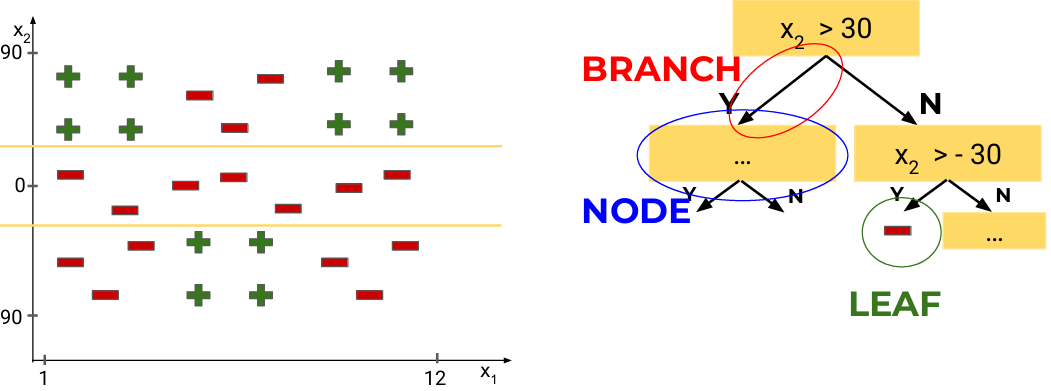
\includegraphics[width=0.6\textwidth]{figuresML/lesson_ml_1_pag_40.png}
\end{center}

More rigorously, we look for the \textbf{split function} $S_{p}(j,t)$ where $j$ is the $j$-th feature and $t$ is the threshold to partition the parent region $R_{p}$:
\begin{equation}
S_{p}(j,t) = ( \{x \ | \ x_{j} < t, x \in R_{p}\} \ , \ \{x \ | \ x_{j} \ge t, x \in R_{p}\} )
\end{equation}
Our objective is reaching \textbf{purity}: we want that at the end of the training, each leaf contains only one class. \\ Given the class $c$, we define $\hat{p}_{c}$ to be the proportion of class k observations (with N observations) in node $m$:
\begin{equation}
\hat{p}_{c} = \frac{1}{N}\sum_{x_{i} \in R_{m}} I(y_{i}=c)
\end{equation}
We then define an impurity measure which gives us an idea of the relative number of points that have been misclassified at each node. For example, we could choose the \textbf{misclassification loss}
\begin{equation}
L_{misclass} = 1 - \max(\hat{p}_{c}) \quad \text{,}
\end{equation}
but we rapidly run into an issue. Take a look at the two different splits below. In the first example the $R_1$ and $R_2$ nodes still contain both - and + values, while in the second one $R_2$ is already a leaf. It should be obvious that the latter is the better choice. However if we compute the weighted mean misclassification loss we get the same value for the two cases: 
\begin{equation*}
\begin{aligned}
    L_1 &= \frac{N_1}{N} L(R_1) + \frac{N_2}{N} L(R_2) = \frac{400}{800}\left(1-\frac{300}{400}\right) + \frac{400}{800}\left(1-\frac{300}{400}\right) = 0.25 \\ 
    L_2 &= \frac{N_1}{N} L(R_1) + \frac{N_2}{N} L(R_2) = \frac{600}{800}\left(1-\frac{400}{600}\right) + \frac{200}{800}\left(1-\frac{200}{200}\right) = 0.25
\end{aligned}
\end{equation*}
\begin{center}
    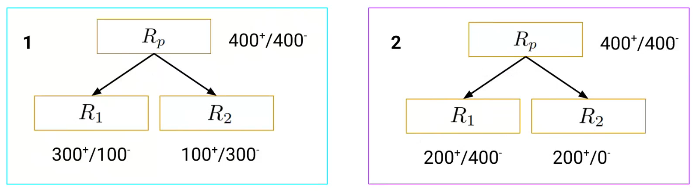
\includegraphics[width=0.6\textwidth]{figuresML/lesson_ml_1_pag_42.png}
\end{center}
We can then use another type of impurity measure, such as the \textbf{Cross-Entropy} 
\begin{equation}
    L_{CE} = -\sum_{c}\hat{p}_{c}\log\hat{p}_{c} 
\end{equation} 
or the \textbf{Gini impurity} 
\begin{equation}
    G = 1 - \sum_{i=1}^{C}p_{i}^{2}
\end{equation} 
Applying the latter in the previous example we get
\begin{equation}
\begin{aligned}
    G_{1} &= \frac{N_1}{N} G(R_1) + \frac{N_2}{N} G(R_2) \\
           &= \frac{400}{800}\left[1-\left(\frac{300}{400}\right)^2-\left(\frac{100}{400}\right)^2\right] + \frac{400}{800}\left[1-\left(\frac{100}{400}\right)^2-\left(\frac{300}{400}\right)^2\right] = 0.375 \\ 
    G_{2} &= \frac{N_1}{N} G(R_1) + \frac{N_2}{N} G(R_2) \\
           &= \frac{600}{800}\left[1-\left(\frac{400}{600}\right)^2-\left(\frac{200}{600}\right)^2\right] + \frac{200}{800}\left[1-\left(\frac{200}{200}\right)^2-\left(\frac{0}{200}\right)^2\right] = 0.333
\end{aligned}
\end{equation}
When computing a decision tree, we compute all the possible impurities in every possible split in order to choose the most efficient way to reach convergence, similarly to the gradient descent method. To sum up, decision trees are easy to explain, interpretable, fast and can handle categorical variables. However they usually have a low predictive accuracy and high variance and of course they are not additive. 

\hrulefill
\\ Note: Scikit-learn library offers many ML techniques implementation in Python. You can find it here: \url{https://scikit-learn.org/stable/index.html}. Here's a representation of different classification methods implemented using this library. 
\begin{center}
    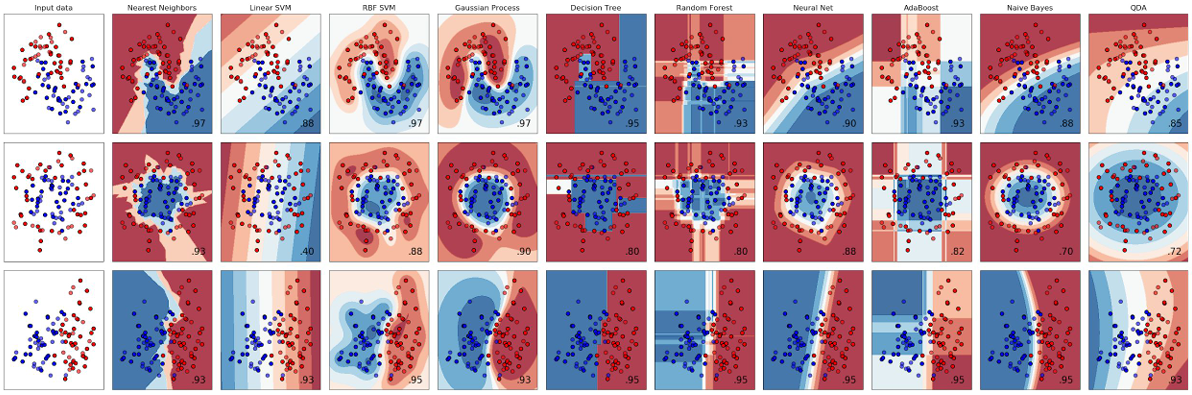
\includegraphics[width=0.9\textwidth]{figuresML/lesson_ml_1_pag_48.png}
\end{center}
\hrulefill

\subsection{Representational learning and Capacity}

Before diving into more complex architectures like Neural Networks, it is crucial to observe the learning process from a more holistic point of view. When we define a specific hypothesis function, we are essentially declaring how we choose to represent our data and our problem (e.g., framing it as a classification task). This "representation" is fundamentally driven by two main factors: the available data and the specific type of algorithm we select.

We can distinguish between two major paradigms based on how this representation is constructed:
\begin{itemize}
    \item[-] \textit{Classical Machine Learning}: In traditional models, the representation heavily relies on human intervention (often referred to as \textit{Feature Engineering}). The algorithm's performance depends on how we manually compute and extract input features or measures from the raw data. For instance, if dealing with a raw time-domain signal, a physicist might first apply a Fourier transform to pass only the relevant frequency amplitudes to a linear classifier. Furthermore, the representation depends on the intrinsic complexity of the chosen mathematical model (e.g., choosing a polynomial model of degree $d$ versus a purely linear one) and its number of free parameters.
    \item[-] \textbf{Deep Learning (Representational Learning)}: In this paradigm, the optimal representation is learned directly and automatically by the model itself. Instead of manually engineering features, we feed raw data to the algorithm and let the training process discover the most useful mathematical transformations to solve the specific problem. A classic example is a Convolutional Neural Network (CNN): we input raw image pixels, and the network learns to represent them hierarchically. It might learn to detect simple edges in its first layers, combine them into shapes in intermediate layers, and finally recognize complex objects in the deepest layers. As with classical ML, the capacity of this learned representation still depends on the number of free parameters available to the network.
\end{itemize}

Different models can represent different types of function, and of course models with more parameters can approximate a larger number of functions. The ability of representing many functions is called \textbf{capacity}, which measures the model's ability to use information effectively (e.g. in a Neural Network: more neurons, more layers $\to$ greater capacity).

With that said, the choice seems simple enough: you should just use the model with the highest capacity to fit the data precisely. Unfortunately, that is horrendously wrong. Our goal is not simply to fit the training data, but to make the algorithm work on unseen ones. In fact, by increasing the number of parameters one could theoretically fit a function for any kind of dataset. The ability of a model to have good performance on unseen data is called \textbf{generalization capability}. 

Take a look at the following figure witch represents a polynomial fitting:
\begin{itemize}
    \item[-] In the first panel the dataset is not fitted properly since the grade of the chosen polynomial is too low. It is a classical case of \textbf{underfitting}.
    \item[-] In the second panel the dataset is perfectly fitted.
    \item[-] In the third panel the dataset is fitted using a high number of parameters: the algorithm has "learned by heart" the training data and it won't work with other samples. We are looking at \textbf{overfitting}
\end{itemize} 

\begin{center}
    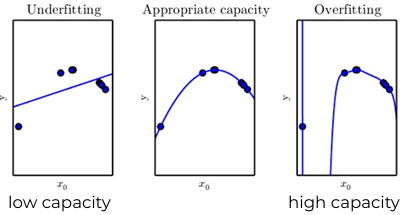
\includegraphics[width=0.4\textwidth]{figuresML/lesson_ml_1_pag_52.png}
\end{center}

The problem is that you will need to program algorithms with millions of parameters and in those cases is not as easy to spot overfitting problems, but there are many methods to try and avoid it. For example, it is standard procedure to split our dataset in a training set and a validation set. We train the algorithm using the first one and then confront its predictions with the validation set, as shown here. 

\begin{center}
    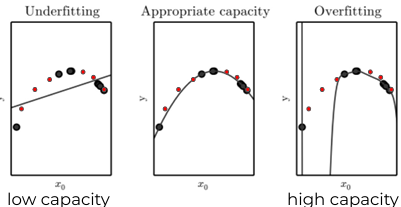
\includegraphics[width=0.4\textwidth]{figuresML/lesson_ml_1_pag_54.png}
\end{center}

Another practical tip when developing very complex models is to start in an underfitting situation and then add parameters until you get out of it. 

Before you go on, make sure that you understood the non trivial link between capacity and generalization.

\subsection{Regularization}
There exist some techniques that help in achieving good performance on data different from the training set even with a high number of parameters known as \textbf{regularization techniques}. Different algorithms need to be regularized in different methods, but many mechanisms can be implemented to the vast majority of them. \\ 
Here are the most common and practical ways:
\begin{itemize}
    \item[-] The cost function can be modified by adding regularization terms
    \item[-] The examples in the training dataset can be increased with \textbf{augmentation techniques}.
    \item[-] \textit{Stochastic noise} can be added to the data.
    \item[-] Existing examples can be transformed with transformations that are known to be invariant for the solution we look for. 
\end{itemize}
One of the most common practice is adding a \textbf{penalty} to the loss function in order to limit some parts of the model parameter space. \\
However, you should be aware of the risks of doing so. Take a look at the following example where we are fitting data using a 5 degrees polynomial $\theta_0 + \theta_1x +...+\theta_5x^5$. The loss function $J(\theta)$ is modified to be $J(\theta) + \sqrt{\lambda||\theta||^{2}}$. As you can see, when $\lambda$ is set to a high value, the easiest way to minimize such function is to set all the parameters $\theta$ to zero, which obviously ruins our fit.

\begin{center}
    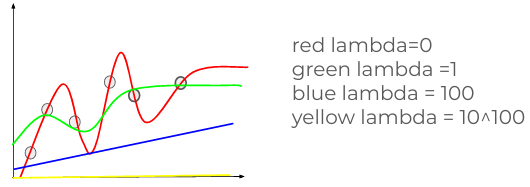
\includegraphics[width=0.55\textwidth]{figuresML/lesson_ml_1_pag_59.png}
\end{center}

\subsection{Data management for model selection}

As mentioned before, we need an intelligent way to divide and use our dataset. A standard practice is dividing the available data into three distinct subsets:
\begin{itemize}
    \item \textbf{Training set}: used for algorithm training and fitting the model's parameters.
    \item \textbf{Validation set}: used to test the algorithm during the training phase, allowing for model selection and tuning without biasing the final evaluation.
    \item \textbf{Test set}: strictly reserved to test the final algorithm's performance on unseen data.
\end{itemize}

An alternative and robust approach is \textbf{K-Fold Cross validation}, which involves dividing the data into multiple folds and iteratively using different combinations of them as training and test data, as shown in the figure below. Variations of this method include \textit{Stratified cross validation} and \textit{Nested Stratified cross validation}.

\begin{center}
    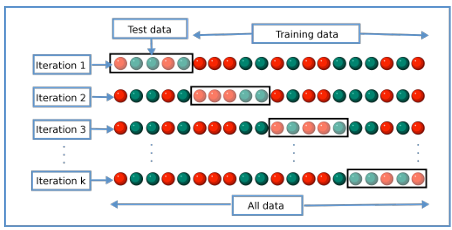
\includegraphics[width=0.7\textwidth]{figuresML/lesson_ml_1_pag_60.png}
\end{center}

\subsection{Hyperparameters optimization}
We have seen that models rely on different hyperparameters. When we develop complex architectures like a Neural Network, we will have many hyperparameters to tune. To search for the best configuration, two common strategies are used (as shown below):
\begin{itemize}
    \item[-] \textbf{Grid Search}: exhaustively evaluating a predefined, regular grid of hyperparameter values.
    \item[-] \textbf{Random Search}: sampling hyperparameter combinations randomly within defined distributions.
\end{itemize}

\begin{center}
    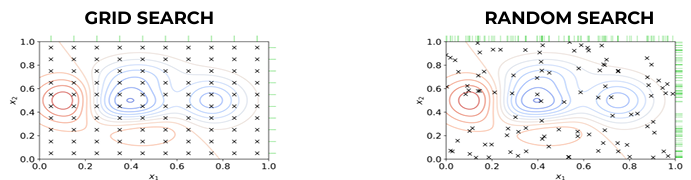
\includegraphics[width=0.85\textwidth]{figuresML/lesson_ml_1_pag_61.png}
\end{center}

\subsection{Metrics}
In the context of machine learning, a \textbf{metric} is a quantifiable measure used to evaluate the performance of a model. While a loss function is used internally by the algorithm during the training phase to update its parameters, a metric is primarily used by developers to interpret how well the model is performing and generalizing on the data (especially on the validation and test sets). It provides a mathematical way to compare the model's predictions against the actual ground truth.

The metric to be used strictly depends on the problem we want to solve and on the distribution of our data.
\begin{itemize}
    \item \textit{Regression}: common metrics include 
    \begin{itemize}
        \item[-] MAE (Mean Absolute Error);
        \item[-] MSE (Mean Squared Error);
        \item[-] RMSE (Root Mean Squared Error).
    \end{itemize}    
    \item \textit{Classification}: common metrics include 
    \begin{itemize}
        \item[-] Accuracy (proportion of correct predictions);
        \item[-] Precision (proportion of true positives among predicted positives);
        \item[-] Recall (or sensitivity, proportion of true positives among actual positives);
        \item[-] F1-score (the harmonic mean of precision and recall);
        \item[-] ROC-AUC (area under the ROC curve for binary classification);
        \item[-] Confusion Matrix (showing TP, FP, FN, TN, see below).
    \end{itemize}
    \item \textit{Segmentation}: common metrics include
    \begin{itemize}
        \item[-] IoU (Intersection over Union, overlap between predicted and true regions);
        \item[-] Dice Coefficient (overlap measure similar to F1 score);
        \item[-] Pixel Accuracy (percentage of correctly classified pixels);
        \item[-] Mean IoU (average IoU across all classes).
    \end{itemize}
\end{itemize}
It is beyond this course to focus on each and everyone of those, but let's look at some important examples.

For a \textit{binary classification} task, the predictions can be summarized in a so called \textbf{Confusion Matrix} comparing the predicted class with the true class (positive or negative). The matrix elements are:
\begin{itemize}
    \item[-] True Positive (TP): correctly predicted positive.
    \item[-] False Negative (FN): incorrectly predicted negative.
    \item[-] False Positive (FP): incorrectly predicted positive.
    \item[-] True Negative (TN): correctly predicted negative.
\end{itemize}
From these, several important metrics can be derived, as shown in the following figure.

\begin{center}
    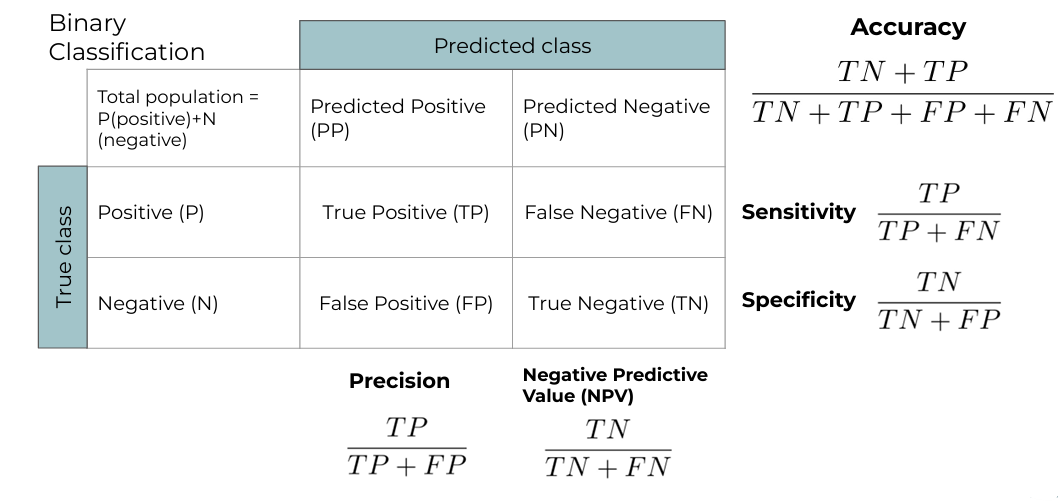
\includegraphics[width=0.85\textwidth]{figuresML/lesson_ml_1_pag_63.png}
\end{center}

For multi-class classification tasks, this concept is naturally extended into a larger, multi-class confusion matrix where the diagonal represents correct predictions.

\begin{center}
    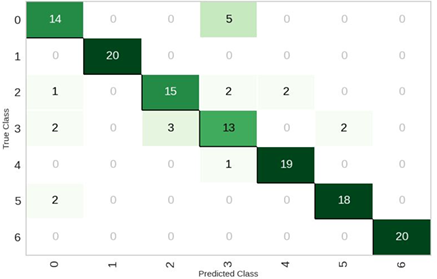
\includegraphics[width=0.55\textwidth]{figuresML/lesson_ml_1_pag_65.png}
\end{center}

We can interpret the output of a classifier as a class probability (this is always true in binary classification, while it depends in multi-class scenarios). The \textbf{ROC curve} (figure below) is constructed by plotting the True positive rate ($\frac{TP}{P}$) on the y-axis against the False positive rate ($\frac{FP}{N}$) on the x-axis for every possible classification threshold. 
\begin{center}
    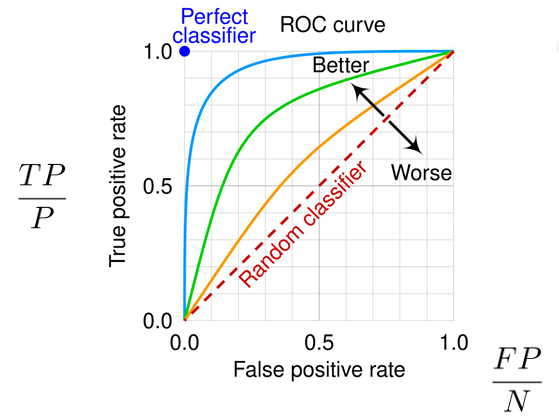
\includegraphics[width=0.45\textwidth]{figuresML/lesson_ml_1_pag_64.png}
\end{center}
To summarize the overall performance of the model into a single scalar value, we compute the \textit{AUC} (Area Under the Curve). The AUC evaluates how well the model can distinguish between classes, regardless of the specific threshold chosen. 
\begin{itemize}
    \item[-] AUC = 1.0: Perfect classifier.
    \item[-] AUC = 0.5: Random classifier (represented by the diagonal line).
\end{itemize}
Probabilistically, the AUC represents the probability that the model will rank a randomly chosen positive instance higher than a randomly chosen negative one. This metric is extremely robust and heavily used in fields like medicine.

For segmentation tasks, evaluating performance pixel-by-pixel can be misleading (as we will see in the prevalence problem). Instead, we often rely on \textbf{overlap measures}. An overlap measure quantifies the spatial agreement between the predicted segmentation mask ($X$) and the ground truth mask ($Y$). Rather than just counting correctly classified pixels, these metrics evaluate how well the shape, size, and position of the predicted object match the real one.

The two most common overlap measures are:
\begin{itemize}
    \item[-] \textbf{Intersection over Union (IoU)} (also known as the Jaccard Index): This metric calculates the area of overlap between the prediction and the ground truth, divided by the total area covered by both combined (their union). It is a strict metric that evaluates the overall spatial correspondence and heavily penalizes both false positives and false negatives.
    $$IoU = \frac{|X \cap Y|}{|X \cup Y|}$$
    
    \item[-] \textbf{Dice Similarity Coefficient (DSC)} (or Dice index): This metric is essentially the F1-score applied to spatial data. It doubles the intersection area and divides it by the sum of the total areas of both masks. While very similar to IoU and perfectly correlated, DSC tends to give slightly more weight to the correctly predicted pixels (the intersection), often resulting in a slightly higher score than IoU for the same prediction.
    $$DSC = \frac{2|X \cap Y|}{|X| + |Y|}$$
\end{itemize}

\textit{Exercise: try to write these two metrics in terms of TP, FP and FN}. \\
Let's solve this exercise to better understand how these metrics relate to the standard confusion matrix. If we consider the overlapping region $X \cap Y$ as the True Positives (TP), the remaining part of the predicted mask as False Positives (FP), and the unpredicted part of the ground truth mask as False Negatives (FN), we can rewrite the formulas as follows:
$$ IoU = \frac{TP}{TP + FP + FN} $$
$$ DSC = \frac{2TP}{2TP + FP + FN} $$

It should be clear that using the wrong metric can be highly deceiving. Here are two cases showing, for example, why accuracy is not always the optimal choice:
\begin{enumerate}
    \item Let's suppose we are solving a binary classification task and our test set classes are \textbf{unbalanced} (e.g., 80 positive and 20 negative). If our classifier stubbornly predicts everything as positive, it is clearly a very bad classifier since it is not differentiating anything at all. However, if we compute the accuracy, we get an impressive 80\%. Thus, we cannot simply use accuracy if our dataset is unbalanced.
    \item Let's try to use accuracy as a metric for a segmentation problem involving tiny objects (a situation typical in medicine). Suppose we have a true segmentation mask and a predicted one, both made of 1000 pixels total, but the target masks are only 10 pixels wide and do not overlap at all. This is undeniably a bad segmentation algorithm. If we compute the DSC, the result is correctly 0. However, if we evaluate the pixel accuracy based on the overwhelming majority of background pixels classified as non-mask, we get an outstanding 99\%.
\end{enumerate}

\section{Intro to Deep Learning and Artificial Neural Networks}

\subsection{Introduction}\label{sec:ML_images}
As mentioned at the beginning of the chapter, deep learning is machine learning made with Deep Neural Networks.

Before starting to dive deeper into DNNs, let's talk for a second about digital images. It should be clear that a 2D Grayscale image is a 2D matrix, so it's a rank-2 tensor with shape (height, width). Instead, an RGB image is a 3D tensor with shape (height, width, channels), where $I(x, y) = [R(x, y), G(x, y), B(x, y)]$. There also exist 3D Grayscale images, which can be seen as a rank-3 tensor with shape (height, width, depth). They are vastly used in medicine, e.g. in computed tomography.

\begin{center}
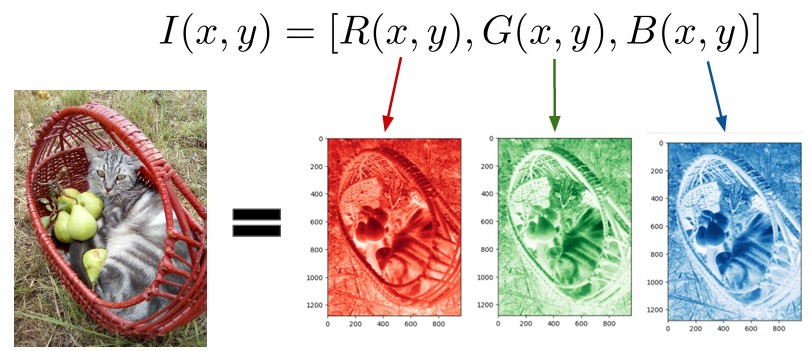
\includegraphics[width=0.6\textwidth]{figuresML/lesson_ml_1_pag_72.png} \\
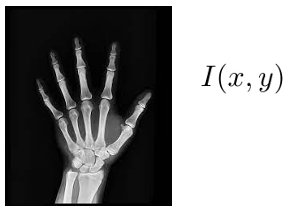
\includegraphics[width=0.25\textwidth]{figuresML/lesson_ml_1_pag_72a.png} \hspace{9mm}
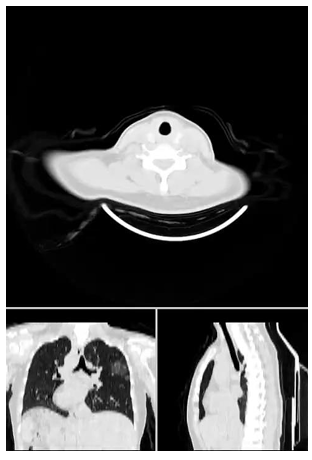
\includegraphics[width=0.25\textwidth]{figuresML/lesson_ml_1_pag_73.png}
\end{center}

\subsection{Logistic regression as a neural network}
Let's try to ease into DL starting from the concepts we are familiar with. Let's say for example that we want to write an algorithm which recognizes whether there is a cat in a given image. In our example (figure below), a $64 \times 64$ image can be flattened into an input vector with components $x_1$ to $x_n$. 
We can apply a linear transformation $wx + b$ followed by a sigmoid function $\sigma$, such that $\hat{y} = \sigma(\theta^T x) = \sigma(wx + b)$. Note that we have changed the notation just a little: the parameters are now called $w$ and not $\theta$ just because in DNNs we usually refer to them as \textbf{weights}.  

\begin{center}
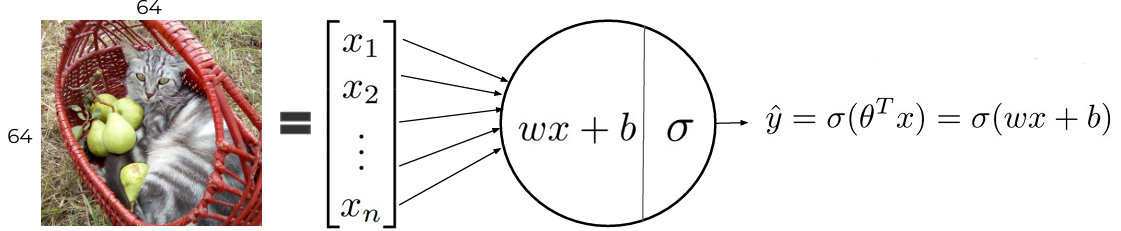
\includegraphics[width=0.85\textwidth]{figuresML/lesson_ml_1_pag_75.png}
\end{center}

We want to train this algorithm by following these steps:
\begin{enumerate}
    \item[-] Initialize weights and bias.
    \item[-] Find the optimal $w, b$.
    \item[-] Use them to predict $y$.
\end{enumerate}
In this case we could use a Binary Cross-Entropy as a loss function: 
\begin{equation}
    L(\theta) = -[y \log \hat{y} + (1-y)\log(1-\hat{y})]
\end{equation}
The output of this algorithm will be 1 if there is a cat, or 0 if there isn't: it should be clear that this is just a binary classification problem.

The circle representation in the figure above is what we call a \textbf{neuron}, and it is made of a \textbf{linear part} and an \textbf{activation function} (the sigmoid in our example). A \textbf{Deep Neural Network} can then be defined as a model composed of many neurons organized in \textbf{layers}.

Let's take another step forward by making our algorithm a little more complicated. Let's say that our goal now is finding a cat, a dog, or a bird in an image. To do so, we shall connect the input vector $x$ to multiple neurons, which we index using square brackets to indicate the layer as in the following figure. Of course, in doing so we are going to need three times the parameters used in the previous model. The activation functions for this first layer are:
\begin{itemize}
    \item[-] $\hat{y}_1 = a_1^{[1]} = \sigma(w_1^{[1]}x + b_1^{[1]})$
    \item[-] $\hat{y}_2 = a_2^{[1]} = \sigma(w_2^{[1]}x + b_2^{[1]})$
    \item[-] $\hat{y}_3 = a_3^{[1]} = \sigma(w_3^{[1]}x + b_3^{[1]})$
\end{itemize}
Each neuron will be responsible for a specific class (e.g., presence of a cat, dog, or bird) and in this case we must change the labels for the output:
\begin{itemize}
    \item[-] $[1, 0, 0]$ for the presence of a cat;
    \item[-] $[0, 1, 0]$ for the presence of a dog;
    \item[-] $[0, 0, 1]$ for the presence of a bird.
\end{itemize}
With this multi-class structure, we define the loss function as 
\begin{equation}\label{eq:4.17}
    L(\theta) = -\sum_{k=1}^{3}[y_k \log \hat{y}_k + (1-y_k)\log(1-\hat{y}_k)]
\end{equation} 
Notice that this is not yet a neural network since each output is totally independent of each other. 

\begin{center}
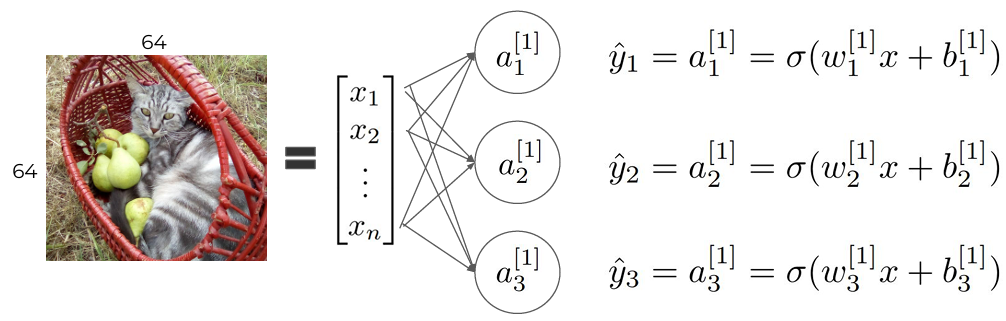
\includegraphics[width=0.85\textwidth]{figuresML/lesson_ml_1_pag_82.png}
\end{center}

Let's change one more time the problem by introducing the constraint that there is strictly a cat, a dog, or a bird. It will be useful to change our notation slightly, as shown in the figure below. We isolate the linear part and write it as such: $z_1^{[1]} = w_1^{[1]}x + b_1^{[1]}$. We also use the \textbf{softmax} function as our activation function:
\begin{equation}
a_1^{[1]} = \frac{e^{z_1^{[1]}}}{\sum_{k=1}^{3}e^{z_k^{[1]}}}
\end{equation}
The softmax introduces a relationship between the 3 neurons so that we obtain a (normalized) probability distribution between the classes instead of an independent probability for each class. For example, if in the image there is a cat with an 80\% probability, there could be a dog with 10\% probability and a bird with another 10\%. In this case, we should also change the output labels to a so-called \textit{one-hot encoding}: $[1, 0, 0]$, $[0, 1, 0]$, $[0, 0, 1]$ are the only possible labels (they do not combine as before). With softmax, we utilize the simpler cross-entropy loss function (since any predicted $y$ depends on all the other values, it is too hard to compute the derivative of Eq. \ref{eq:4.17}):
\begin{equation}
    L_{CE} = -\sum_{k=1}^{3} y_k \log(\hat{y}_k)
\end{equation}
Since there is a relationship between all the outputs, \textit{this is the first shallow example of a neural network}.

\begin{center}
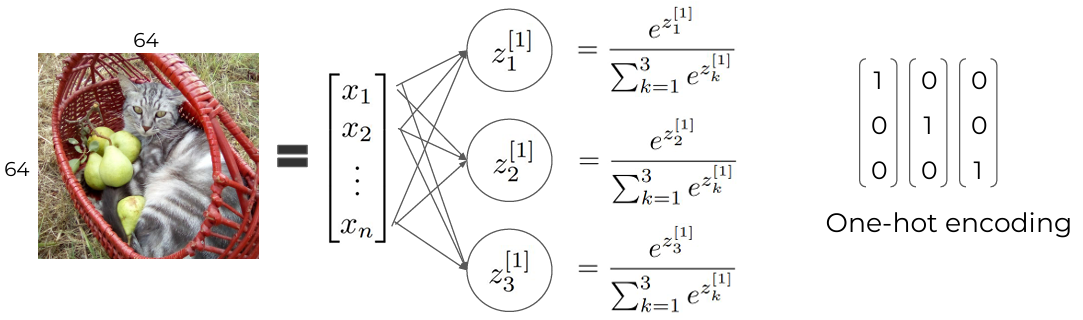
\includegraphics[width=0.85\textwidth]{figuresML/lesson_ml_1_pag_88.png}
\end{center}

\subsection{Neural Network architecture}
The following figure can be useful to understand the typical architecture of a neural network. First, the inputs $x$ are connected to the first layer of neurons called the \textbf{input layer}. Then all the neurons of the input layer are connected to all the neurons of the subsequent layer, creating a \textbf{fully connected layer}. The last layer is also called an \textbf{output layer} and all the layers which are not the input nor the output are called \textbf{hidden layers}. It should be clear now that a layer refers to neurons that are not connected to each other within the same depth level. When you build an architecture, the number of neurons in the output layer should match your problem, i.e., it should be equal to the number of classes: it usually defines the problem we would like to solve.

\begin{center}
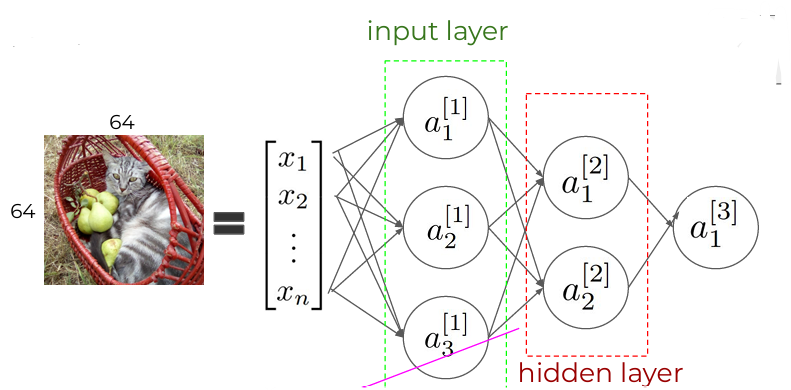
\includegraphics[width=0.75\textwidth]{figuresML/lesson_ml_1_pag_90.png}
\end{center}

Now, the learning scheme is quite the same as in the case of linear regression we have seen at the beginning of the chapter: at a certain point we will find a loss function and use the gradient descent method to minimize it. The difference is that before doing this, we need to pass through the entire structure of our neural network. The process works through \textbf{forward propagation}: we process the input data according to the operation of the neuron sequentially (i.e. the last activation will be a function of the last $z$, which is a function of the previous activation, and so on), as shown below. 

\begin{center}
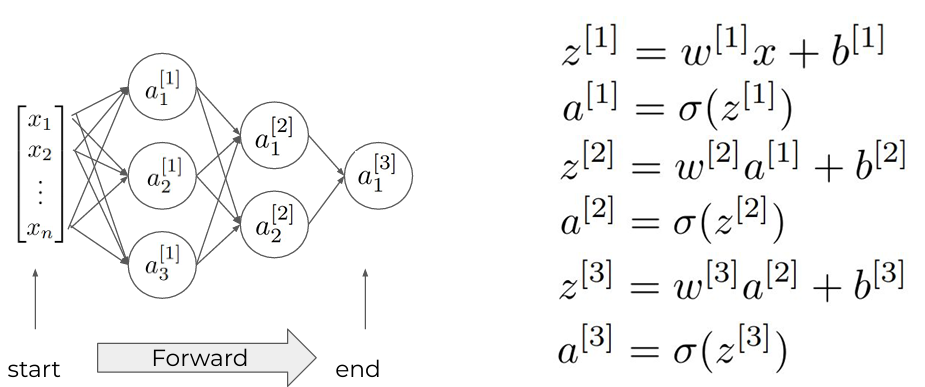
\includegraphics[width=0.75\textwidth]{figuresML/lesson_ml_1_pag_93.png}
\end{center}

Once we have computed the activation of the last layer, we have our prediction so we can compute the value of the loss function. To minimize this loss function using an optimization algorithm like Stochastic Gradient Descent, we need to \textbf{compute the derivatives of the loss function with respect to all the network weights}. 

As an example, let's try to do it explicitly for our neural network. Since it has only one neuron in the last layer, we are obviously trying to solve a binary classification task, so we will use the BCE as a loss function.

To clarify the notation:
\begin{itemize}
    \item[-] By \textit{cost function} we mean all the loss functions computed on a dataset ($m$ is the batch size): $J(\hat{y}, y) = \frac{1}{m}\sum_{i=1}^{m}L^{(i)}(\hat{y}, y)$.
    \item[-] By \textit{loss function} we mean the single error computation, e.g. BCE: \\ $L^{(i)} = -[y^{(i)}\log\hat{y}^{(i)} + (1-y^{(i)})\log(1-\hat{y}^{(i)})]$.
\end{itemize}
We compute the derivative of the loss with respect to $w^{[3]}$:
\begin{equation*}
    \frac{\partial L}{\partial w^{[3]}} = -\left[ y^{(i)} \frac{\partial}{\partial w^{[3]}} (\log(\sigma(w^{[3]}a^{[2]} + b^{[3]}))) + (1 - y^{(i)}) \frac{\partial}{\partial w^{[3]}} (\log(1 - \sigma(w^{[3]}a^{[2]} + b^{[3]}))) \right]
\end{equation*}
which, after a few simple mathematical steps becomes:
\begin{equation}
\frac{\partial L}{\partial w^{[3]}} = -(y^{(i)} - a^{[3]})a^{[2]}
\end{equation}
Using the chain rule, we can compute the derivative with respect to $w^{[2]}$:
\begin{equation*}
\frac{\partial L}{\partial w^{[2]}} = \frac{\partial L}{\partial a^{[3]}} \frac{\partial a^{[3]}}{\partial z^{[3]}} \frac{\partial z^{[3]}}{\partial a^{[2]}} \frac{\partial a^{[2]}}{\partial z^{[2]}} \frac{\partial z^{[2]}}{\partial w^{[2]}}
\end{equation*}
We know exactly how to compute each of those partial derivatives because we have
\begin{equation}
\begin{aligned}
z^{[1]} &= w^{[1]}x + b^{[1]} \quad \quad \ \  a^{[1]} = \sigma(z^{[1]}) \\
z^{[2]} &= w^{[2]}a^{[1]} + b^{[2]} \quad\quad a^{[2]} = \sigma(z^{[2]}) \\
z^{[3]} &= w^{[3]}a^{[2]} + b^{[3]} \quad\quad a^{[3]} = \sigma(z^{[3]})
\end{aligned}
\end{equation}
We also know that the derivative of the sigmoid is nicely defined as $g'(z) = g(z)(1-g(z))$, so 
\begin{equation*}
    \dfrac{\partial a^{[i]}}{\partial z^{[i]}} = a^{[i]}(1-a^{[i]})  
\end{equation*}
Lastly: 
\begin{equation*}
    \frac{\partial L}{\partial a^{[3]}} \frac{\partial a^{[3]}}{\partial z^{[3]}} = \dfrac{\partial L}{\partial z^{[3]}}=\dfrac{\partial L}{\partial w^{[3]}} / \dfrac{\partial z^{[3]}}{\partial w^{[3]}}
\end{equation*}
Putting everything together we get:
\begin{equation}
    \frac{\partial L}{\partial w^{[2]}} = w^{[3]} a^{[2]} (1 - a^{[2]}) (a^{[3]} - y^{(i)}) a^{[1]}
\end{equation}

The same thing can be done for $\dfrac{\partial L}{\partial w^{[1]}}$. This kind of derivative computation for the loss function is called \textbf{backpropagation} and it is extremely efficient because many terms of the derivatives are already computed in the forward pass (like $a^{[1]}$, $a^{[2]}$, $a^{[3]}$) or in the previous derivatives. Caching them makes backpropagation computationally convenient. 

With that said, we have a pretty good understanding of the training cycle of a neural network: 
\begin{enumerate}
    \item Forward pass of the data
    \item Computation of the loss function
    \item Computation of the derivatives of the loss function through backpropagation
    \item Minimization of the loss function and optimization of the weights (e.g through SGD)
    \item Repeat until convergence
\end{enumerate}
An entire pass of the training dataset through the learning algorithm (1-4) is called an \textbf{epoch}.
We can update the network in different ways during training:
\begin{enumerate}
    \item Update the weights for each training point (very time consuming).
    \item Update the weights for a mini-batch of data (less time consuming).
\end{enumerate}

\hrulefill

\subsubsection{Note: A very brief and incomplete history of NN}
Machine learning systems have been around for many years, but what has changed nowadays is the arrival of Deep Learning! The history of AI is characterized by periods of time often referred to as \textit{AI winters} where technology could not keep up with theory, as the computational power available was not enough for machine learning purposes.  Here are some meaningful milestones:
\begin{itemize}
    \item[-] 1957 - Rosenblatt introduces the \textit{perceptron} (see below).
    \item[-] 1962 - Rosenblatt used the term backpropagation which will become the mathematical algorithm for doing feedback in practice.
    \item[-] 1980 - Fukushima introduces the \textit{neocognitron}.
    \item[-] 1998 - LeCun published the first Neural Network that is able to work directly with images!
    \item[-] 2006 - Chellapilla proposed using GPUs to boost NN training.
    \item[-] 2006 - 2012 - Many technologies evolved, the amount of available data increased until 2012 when something very interesting happened (we will soon see).
\end{itemize}
\hrulefill

\subsection{Multi-Layer Perceptron and Deep Feed Forward Network}
The most common NN in the '90s was the \textbf{Multilayer Perceptron} (MLP). 
It features a graph structure organized in 3 layers (input, hidden and output), whose nodes are connected only from one layer to the next and all possible connections are present (fully connected), as shown below. There are no intra-layer connections and no direct connections from input to output. Size of input and output layers are fixed by the problem. Hyperparameters include the size of the hidden layers and the type of activation function, while the parameters to learn are the weights of the connections. It is nothing stranger than the simple example we have seen before.

\begin{center}
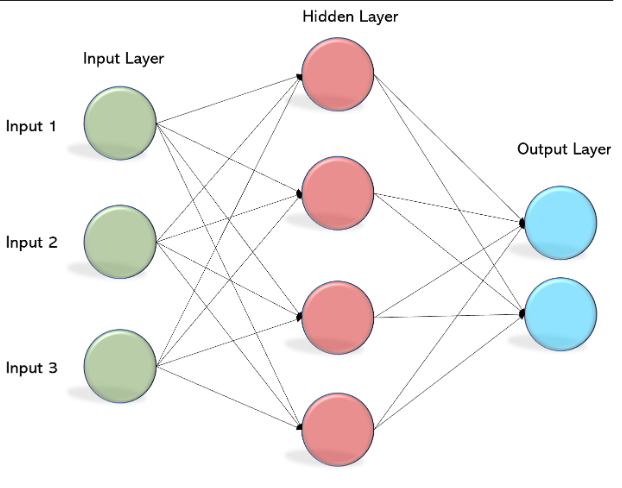
\includegraphics[width=0.4\textwidth]{figuresML/lesson_ml_1_pag_111.png}
\end{center}

The simplest extension to the MLP is to add more hidden layers (even hundreds or thousands), forming a \textbf{Deep Feed Forward Network} (or \textit{Deep Dense Network}). The hierarchical structure allows easier abstraction by the network, with early layers computing low-level features and deeper layers representing more abstract properties.

\begin{center}
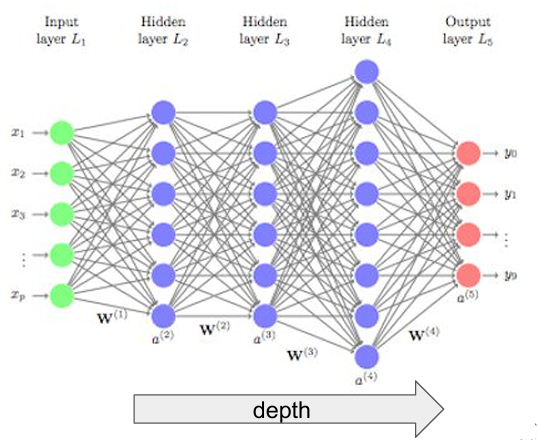
\includegraphics[width=0.65\textwidth]{figuresML/lesson_ml_1_pag_113.png}
\end{center}

\subsection{The importance of activation functions}
Let's now take a step back and ask ourselves: \textit{why do we need activation functions?} The "horse" problem shown below illustrates what happens if we do not use an activation function in a Neural Network i.e., if we do not introduce non-linearity. If we train a linear classifier on images of horses facing left or right, the learned weights look like a two-headed horse. There are no two-headed horses! \textbf{Non-linearity is required} (we will see why more thoroughly in Sec. \ref{sec:non_linearity}.

\begin{center}
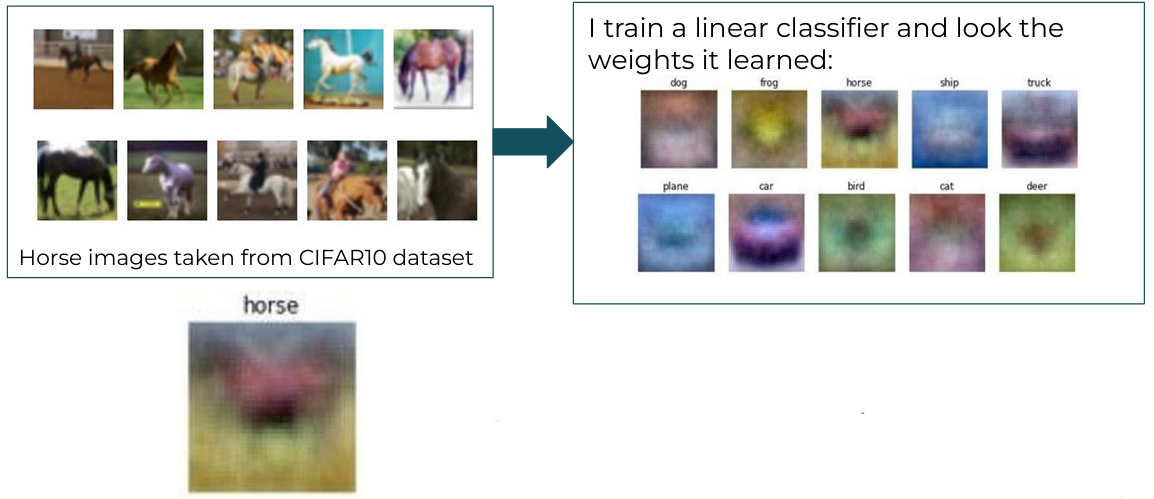
\includegraphics[width=0.9\textwidth]{figuresML/lesson_ml_1_pag_115.png}
\end{center}

There are many different activation functions:
\begin{itemize}
    \item[-] \textit{Linear}: $f(x) = x$. Of course it cannot be used in hidden layers (where non-linearity is mandatory) but it can be useful for output nodes in regression problems if the output values span a very wide range.
    \item[-] \textbf{Sigmoid}: $f(x) = \sigma(x) = \frac{1}{1+e^{-x}}$. It was used historically in hidden layers but leads to the \textit{vanishing gradient} problem. It can be useful in the last layer for binary classification problems with a single output or multi-label classifiers.
    \item[-] \textbf{Softmax}: $f_i(\vec{x}) = \frac{e^{x_i}}{\sum_{j=1}^{J}e^{x_j}}$. As seen, it is useful in classification problems with one-hot encoded multi-class labels.
    \item[-] \textbf{Rectified Linear Unit (ReLU)}: $f(x) = \max(0, x)$. It is usually the default for hidden layer activations (we will soon see why). Variants of ReLU include Leaky ReLU, Swish and Exponential Linear Unit (ELU).
    \item[-] \textit{tanh}: It is not widely used anymore, even though it was historically relevant.
    \item[-] \textit{Maxout}: $\max(w_1^T x + b_1, w_2^T x + b_2)$
\end{itemize}

\begin{center}
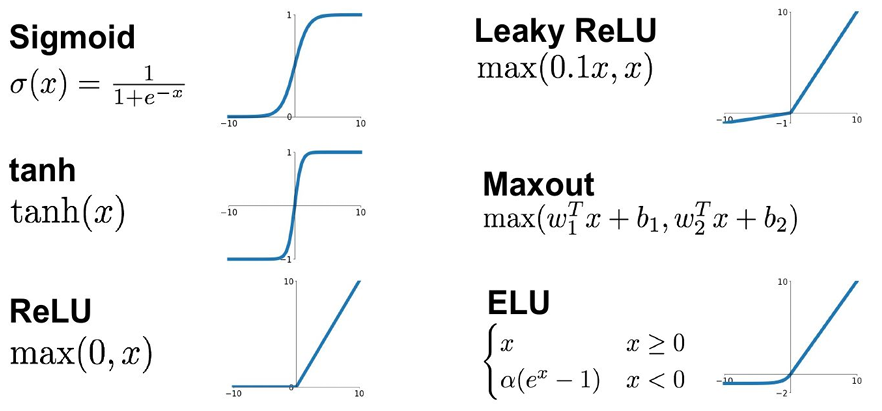
\includegraphics[width=0.65\textwidth]{figuresML/lesson_ml_1_pag_116.png}
\end{center}

It should be clear now that the choice of the activation function for the output layer is pivotal. Here we sum up the correct activation function, loss function, and output label for the three kinds of simple problems we have faced:
\begin{itemize}
    \item[-] \underline{Regression}: Since we want to have a continuous output, we use a linear activation. Loss: Mean Squared Error (MSE) or Mean Absolute Error (MAE). Label: continuous numbers.
    \item[-] \underline{Binary Classification}: We use a Sigmoid activation. Loss: Binary Cross-Entropy. Label: 0 or 1.
    \item[-] \underline{Multi-class Classification}: We use a Softmax activation. Loss: Categorical Cross-Entropy (or Sparse Categorical Cross-Entropy if labels are integers). Label: one-hot for CCE, integers for SCCE (0, 1, 2, 3, ...). Note that it is always better to use one-hot encoding for multi-class classification.
\end{itemize}

\subsection{A deeper look at overfitting and regularization}
As discussed previously, if the capacity is large enough the network could overfit on the training dataset. We must have a separate, statistically independent, validation/generalization sample to evaluate performance (with loss or other metrics). It should also be noticed that training results depend on many choices like the size of the data batches (usually limited by the memory of your GPU), learning rate (how much you move along the gradient at each iteration), chosen gradient descent algorithm, and capacity of the network. Take a look at the following figures to see what could really happen to your loss function during training (there is noise, a loss that dramatically increases at a certain point without a clear reason, and much more).

\begin{center}
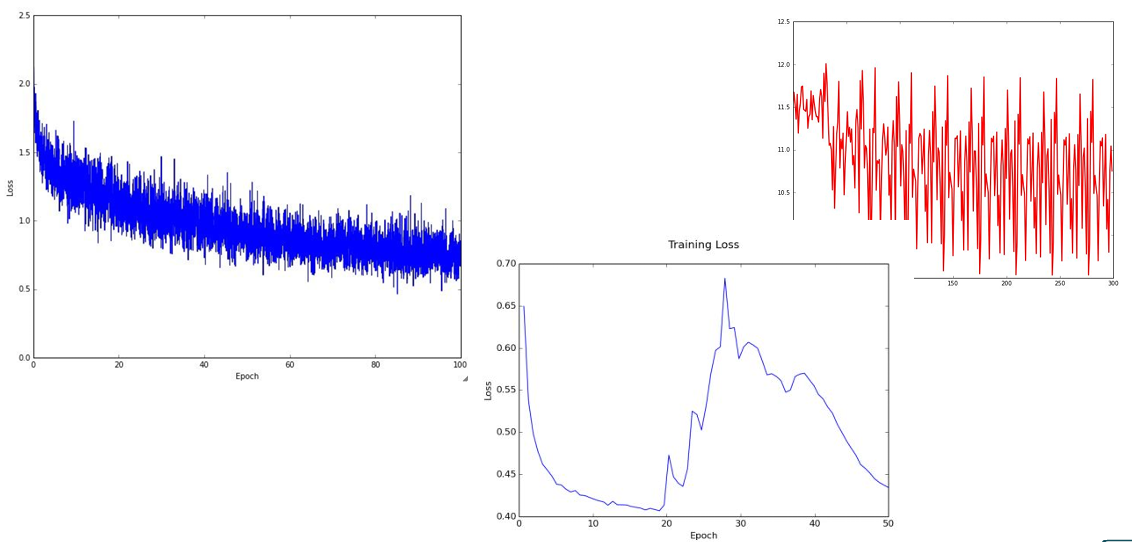
\includegraphics[width=0.65\textwidth]{figuresML/lesson_ml_1_pag_124.png}
\end{center}

Previously, we saw that adding a penalty to the loss function can induce regularization. 
A technique particularly suited for Fully Connected Neural Networks is called \textbf{dropout}: during training a fraction of nodes is discarded randomly at each iteration in order to "confuse" our algorithm. This makes the NN more robust to noise and effectively augments the input dataset, as shown below.

\begin{center}
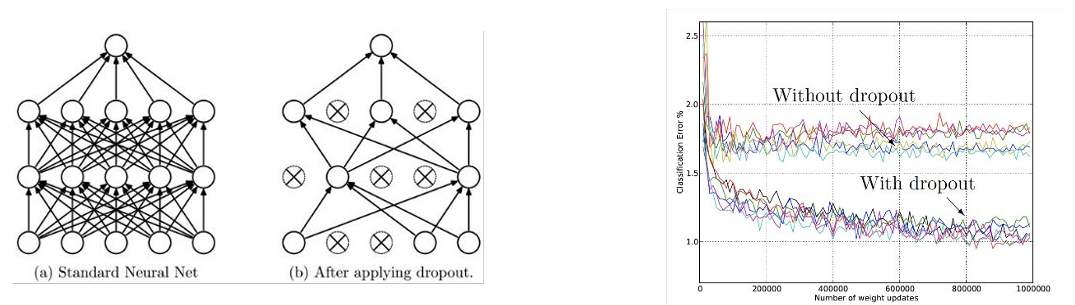
\includegraphics[width=0.95\textwidth]{figuresML/lesson_ml_1_pag_125.png}
\end{center}

As previously mentioned, weight updates can be performed for individual training points or across mini-batches of data. In the context of mini-batch training, \textbf{Batch Normalization (BN)} is a crucial technique designed to normalize the inputs of each hidden layer, ensuring they maintain a stable distribution throughout the training process. 

Specifically, BN calculates the mean and variance for the current mini-batch and uses them to center and scale the layer's activations. 

By keeping the input distribution relatively constant (mitigating a phenomenon known as \textit{internal covariate shift}) each layer does not have to continuously adapt to the changing weights of previous layers. This stability significantly speeds up convergence, allows for the use of much higher learning rates without the risk of divergence, and acts as a mild form of regularization (often reducing the need for techniques like dropout), ultimately leading to improved model generalization.

Proper scaling of input data is a mandatory preprocessing step when training neural networks. Unlike algorithms such as decision trees, where unscaled data merely shifts the split thresholds, neural networks are highly sensitive to input magnitudes. In other words, if the input values $z$ are too large or too small, they can cause activation functions (such as ReLU) to produce extreme outputs. This leads to \textit{network saturation}, a state where neurons lose their sensitivity to the data and effectively "die". If this saturation is allowed to propagate through the network's hidden layers, the model becomes completely untrainable. 

To prevent this and ensure all features operate within the same range, \textbf{input normalization or scaling} is strictly required. The most common approach is \textit{standardization}, which consists of centering the data by subtracting the mean and scaling it by dividing by the standard deviation.

\subsection{Introduction to Keras}
\textbf{Keras} is a Python library that allows you to build, train, and evaluate NNs. Nowadays the most used library is \texttt{torch} because GPT, Transformers and more complex architectures are written with it, and because it seems to be more efficient than \texttt{TensorFlow} (which Keras is a part of). However, in this kind of problem it is very hard to measure the actual efficiency (we will see why). 

Two different syntax methods are usable in Keras to build the network architecture:
\begin{itemize}
    \item[-] \textbf{Sequential}: simple "stack" of layers.
    \item[-] \textbf{Model (functional API)}: create more complex topologies.
\end{itemize}
Multiple types of layers are supported: \textit{dense} (classic fully connected layer), \textit{convolutional}, \textit{recurrent} and so on (we will see those too). It also provides multiple types of activation functions, various optimizers, and gradient descent techniques. Right now most programmers are using \textit{Adam}, which is a particular type of gradient descent algorithm (yes, this too will be a future topic of discussion). 

Below you can find some simple examples to start becoming familiar with this new module.

\subsubsection{- Keras first sequential example}

Here is how you can define a simple sequential model:

\begin{Verbatim}[label=\makebox{\url{https://github.com/lucabaldini/cmepda/tree/master/slides/latex/snippets/pima_classifier.py}},commandchars=\\\{\}]
\PY{c+c1}{\PYZsh{} Necessary modules}
\PY{k+kn}{from}\PY{+w}{ }\PY{n+nn}{numpy}\PY{+w}{ }\PY{k+kn}{import} \PY{n}{loadtxt}
\PY{k+kn}{from}\PY{+w}{ }\PY{n+nn}{keras}\PY{n+nn}{.}\PY{n+nn}{models}\PY{+w}{ }\PY{k+kn}{import} \PY{n}{Sequential}
\PY{k+kn}{from}\PY{+w}{ }\PY{n+nn}{keras}\PY{n+nn}{.}\PY{n+nn}{layers}\PY{+w}{ }\PY{k+kn}{import} \PY{n}{Dense}

\PY{c+c1}{\PYZsh{} Dataset taken from txt}
\PY{n}{dataset}\PY{o}{=}\PY{n}{loadtxt}\PY{p}{(}\PY{l+s+s1}{\PYZsq{}}\PY{l+s+s1}{pima\PYZus{}indians\PYZus{}diabetes.csv}\PY{l+s+s1}{\PYZsq{}}\PY{p}{,} \PY{n}{delimiter}\PY{o}{=}\PY{l+s+s1}{\PYZsq{}}\PY{l+s+s1}{,}\PY{l+s+s1}{\PYZsq{}}\PY{p}{)}
\PY{n}{x}\PY{o}{=}\PY{n}{dataset}\PY{p}{[}\PY{p}{:}\PY{p}{,}\PY{l+m+mi}{0}\PY{p}{:}\PY{l+m+mi}{8}\PY{p}{]}
\PY{n}{y}\PY{o}{=}\PY{n}{dataset}\PY{p}{[}\PY{p}{:}\PY{p}{,}\PY{l+m+mi}{8}\PY{p}{]}

\PY{c+c1}{\PYZsh{} Building a fully connected NN in a sequential way }
\PY{c+c1}{\PYZsh{} (Note which activation function we are using)}
\PY{n}{model} \PY{o}{=} \PY{n}{Sequential}\PY{p}{(}\PY{p}{)}
\PY{n}{model}\PY{o}{.}\PY{n}{add}\PY{p}{(}\PY{n}{Dense}\PY{p}{(}\PY{l+m+mi}{12}\PY{p}{,} \PY{n}{input\PYZus{}dim}\PY{o}{=}\PY{l+m+mi}{8}\PY{p}{,} \PY{n}{activation}\PY{o}{=}\PY{l+s+s1}{\PYZsq{}}\PY{l+s+s1}{relu}\PY{l+s+s1}{\PYZsq{}}\PY{p}{)}\PY{p}{)}
\PY{n}{model}\PY{o}{.}\PY{n}{add}\PY{p}{(}\PY{n}{Dense}\PY{p}{(}\PY{l+m+mi}{8}\PY{p}{,} \PY{n}{activation}\PY{o}{=}\PY{l+s+s1}{\PYZsq{}}\PY{l+s+s1}{relu}\PY{l+s+s1}{\PYZsq{}}\PY{p}{)}\PY{p}{)}
\PY{n}{model}\PY{o}{.}\PY{n}{add}\PY{p}{(}\PY{n}{Dense}\PY{p}{(}\PY{l+m+mi}{1}\PY{p}{,} \PY{n}{activation}\PY{o}{=}\PY{l+s+s1}{\PYZsq{}}\PY{l+s+s1}{sigmoid}\PY{l+s+s1}{\PYZsq{}}\PY{p}{)}\PY{p}{)}

\PY{c+c1}{\PYZsh{} Compiling the model using Adam as optimizer and accuracy as metric}
\PY{n}{model}\PY{o}{.}\PY{n}{compile}\PY{p}{(}\PY{n}{loss}\PY{o}{=}\PY{l+s+s1}{\PYZsq{}}\PY{l+s+s1}{binary\PYZus{}crossentropy}\PY{l+s+s1}{\PYZsq{}}\PY{p}{,} \PY{n}{optimizer}\PY{o}{=}\PY{l+s+s1}{\PYZsq{}}\PY{l+s+s1}{adam}\PY{l+s+s1}{\PYZsq{}}\PY{p}{,} \PY{n}{metrics}\PY{o}{=}\PY{p}{[}\PY{l+s+s1}{\PYZsq{}}\PY{l+s+s1}{accuracy}\PY{l+s+s1}{\PYZsq{}}\PY{p}{]}\PY{p}{)}

\PY{c+c1}{\PYZsh{} Fitting our model in 150 epochs and using batches of data}
\PY{n}{model}\PY{o}{.}\PY{n}{fit}\PY{p}{(}\PY{n}{x}\PY{p}{,}\PY{n}{y}\PY{p}{,} \PY{n}{epochs}\PY{o}{=}\PY{l+m+mi}{150}\PY{p}{,} \PY{n}{batch\PYZus{}size}\PY{o}{=}\PY{l+m+mi}{10}\PY{p}{)}
\PY{n}{\PYZus{}}\PY{p}{,} \PY{n}{accuracy} \PY{o}{=} \PY{n}{model}\PY{o}{.}\PY{n}{evaluate}\PY{p}{(}\PY{n}{x}\PY{p}{,}\PY{n}{y}\PY{p}{)}
\PY{n+nb}{print}\PY{p}{(}\PY{l+s+s1}{\PYZsq{}}\PY{l+s+s1}{Accuracy: }\PY{l+s+si}{\PYZpc{}f}\PY{l+s+s1}{\PYZsq{}} \PY{o}{\PYZpc{}}\PY{p}{(}\PY{n}{accuracy}\PY{o}{*}\PY{l+m+mi}{100}\PY{p}{)}\PY{p}{)}

\end{Verbatim}

\begin{Verbatim}[fontsize=\footnotesize, label=\makebox{\url{https://github.com/lucabaldini/cmepda/tree/master/slides/latex/snippets/pima_classifier.py}},commandchars=\\\{\}]
[Output]
> python pima_classifier.py
Epoch 1/150
77/77 [==============================] - 1s 2ms/step - loss: 1.9542 - accuracy: 0.5286
...
Epoch 150/150
77/77 [==============================] - 0s 2ms/step - loss: 0.4678 - accuracy: 0.7773
24/24 [==============================] - 0s 1ms/step - loss: 0.4531 - accuracy: 0.7812
Accuracy: 78.125000
\end{Verbatim}

\subsubsection{- Keras Functional API:}
A NN can also be seen as the composition of multiple functions (one per layer). A simple stack is $y = f_5(f_4(f_3(f_2(f_1(x)))))$ and a more complex structure could be $y = f_4(f_2(f_1(x)), f_3(x))$. 
The \textit{functional API} allows us to express the idea that each layer is evaluated on the output of a previous layer, as shown here. Take a look at the \texttt{summary} of the NN, which explains its structure.

\begin{Verbatim}[label=\makebox{\url{https://github.com/lucabaldini/cmepda/tree/master/slides/latex/snippets/functional_api_example.py}},commandchars=\\\{\}]
\PY{k+kn}{from}\PY{+w}{ }\PY{n+nn}{keras}\PY{n+nn}{.}\PY{n+nn}{layers}\PY{+w}{ }\PY{k+kn}{import} \PY{n}{Input}\PY{p}{,} \PY{n}{Dense}\PY{p}{,} \PY{n}{concatenate}
\PY{k+kn}{from}\PY{+w}{ }\PY{n+nn}{keras}\PY{n+nn}{.}\PY{n+nn}{models}\PY{+w}{ }\PY{k+kn}{import} \PY{n}{Model}

\PY{c+c1}{\PYZsh{} Defining the input tensor}
\PY{n}{x} \PY{o}{=} \PY{n}{Input}\PY{p}{(}\PY{n}{shape}\PY{o}{=}\PY{p}{(}\PY{l+m+mi}{8}\PY{p}{,}\PY{p}{)}\PY{p}{)}

\PY{c+c1}{\PYZsh{} Example 1: Simple stack structure, y = f3(f2(f1(x)))}

\PY{n}{f1} \PY{o}{=} \PY{n}{Dense}\PY{p}{(}\PY{l+m+mi}{12}\PY{p}{,} \PY{n}{activation}\PY{o}{=}\PY{l+s+s1}{\PYZsq{}}\PY{l+s+s1}{relu}\PY{l+s+s1}{\PYZsq{}}\PY{p}{)}\PY{p}{(}\PY{n}{x}\PY{p}{)}
\PY{n}{f2} \PY{o}{=} \PY{n}{Dense}\PY{p}{(}\PY{l+m+mi}{8}\PY{p}{,} \PY{n}{activation}\PY{o}{=}\PY{l+s+s1}{\PYZsq{}}\PY{l+s+s1}{relu}\PY{l+s+s1}{\PYZsq{}}\PY{p}{)}\PY{p}{(}\PY{n}{f1}\PY{p}{)}
\PY{n}{y\PYZus{}simple} \PY{o}{=} \PY{n}{Dense}\PY{p}{(}\PY{l+m+mi}{1}\PY{p}{,} \PY{n}{activation}\PY{o}{=}\PY{l+s+s1}{\PYZsq{}}\PY{l+s+s1}{sigmoid}\PY{l+s+s1}{\PYZsq{}}\PY{p}{)}\PY{p}{(}\PY{n}{f2}\PY{p}{)}

\PY{c+c1}{\PYZsh{} Creating the model linking input to output}
\PY{n}{model\PYZus{}simple} \PY{o}{=} \PY{n}{Model}\PY{p}{(}\PY{n}{inputs}\PY{o}{=}\PY{n}{x}\PY{p}{,} \PY{n}{outputs}\PY{o}{=}\PY{n}{y\PYZus{}simple}\PY{p}{)}

\PY{c+c1}{\PYZsh{} Example 2: Complex Structure with branches, y = f4( f2(f1(x)), f3(x) )}

\PY{c+c1}{\PYZsh{} Branch 1: f2(f1(x))}
\PY{n}{f1\PYZus{}x} \PY{o}{=} \PY{n}{Dense}\PY{p}{(}\PY{l+m+mi}{12}\PY{p}{,} \PY{n}{activation}\PY{o}{=}\PY{l+s+s1}{\PYZsq{}}\PY{l+s+s1}{relu}\PY{l+s+s1}{\PYZsq{}}\PY{p}{)}\PY{p}{(}\PY{n}{x}\PY{p}{)}
\PY{n}{f2\PYZus{}f1\PYZus{}x} \PY{o}{=} \PY{n}{Dense}\PY{p}{(}\PY{l+m+mi}{8}\PY{p}{,} \PY{n}{activation}\PY{o}{=}\PY{l+s+s1}{\PYZsq{}}\PY{l+s+s1}{relu}\PY{l+s+s1}{\PYZsq{}}\PY{p}{)}\PY{p}{(}\PY{n}{f1\PYZus{}x}\PY{p}{)}

\PY{c+c1}{\PYZsh{} Branch 2: f3(x)}
\PY{n}{f3\PYZus{}x} \PY{o}{=} \PY{n}{Dense}\PY{p}{(}\PY{l+m+mi}{8}\PY{p}{,} \PY{n}{activation}\PY{o}{=}\PY{l+s+s1}{\PYZsq{}}\PY{l+s+s1}{relu}\PY{l+s+s1}{\PYZsq{}}\PY{p}{)}\PY{p}{(}\PY{n}{x}\PY{p}{)}

\PY{c+c1}{\PYZsh{} Combine the two branches (passing them as a list)}
\PY{n}{merged} \PY{o}{=} \PY{n}{concatenate}\PY{p}{(}\PY{p}{[}\PY{n}{f2\PYZus{}f1\PYZus{}x}\PY{p}{,} \PY{n}{f3\PYZus{}x}\PY{p}{]}\PY{p}{)}

\PY{c+c1}{\PYZsh{} Final layer: f4 applied to the merged tensors}
\PY{n}{y\PYZus{}complex} \PY{o}{=} \PY{n}{Dense}\PY{p}{(}\PY{l+m+mi}{1}\PY{p}{,} \PY{n}{activation}\PY{o}{=}\PY{l+s+s1}{\PYZsq{}}\PY{l+s+s1}{sigmoid}\PY{l+s+s1}{\PYZsq{}}\PY{p}{)}\PY{p}{(}\PY{n}{merged}\PY{p}{)}

\PY{c+c1}{\PYZsh{} Create the complex model}
\PY{n}{model\PYZus{}complex} \PY{o}{=} \PY{n}{Model}\PY{p}{(}\PY{n}{inputs}\PY{o}{=}\PY{n}{x}\PY{p}{,} \PY{n}{outputs}\PY{o}{=}\PY{n}{y\PYZus{}complex}\PY{p}{)}

\PY{c+c1}{\PYZsh{} Print a summary to verify the architecture}
\PY{n}{model\PYZus{}complex}\PY{o}{.}\PY{n}{summary}\PY{p}{(}\PY{p}{)}
\end{Verbatim}

\begin{Verbatim}[fontsize=\footnotesize, label=\makebox{\url{https://github.com/lucabaldini/cmepda/tree/master/slides/latex/snippets/functional_api_exampleb.py}},commandchars=\\\{\}]
[Output]
> python functional_api_example.py
Model: "model_1"
_____________________________________________________________________________________
 Layer (type)                   Output Shape         Param #     Connected to                     
=====================================================================================
 input_1 (InputLayer)           [(None, 8)]          0           []                               
                                                                                                  
 dense_3 (Dense)                (None, 12)           108         ['input_1[0][0]']                
                                                                                                  
 dense_4 (Dense)                (None, 8)            104         ['dense_3[0][0]']                
                                                                                                  
 dense_5 (Dense)                (None, 8)            72          ['input_1[0][0]']                
                                                                                                  
 concatenate (Concatenate)      (None, 16)           0           ['dense_4[0][0]',                
                                                                  'dense_5[0][0]']                
                                                                                                  
 dense_6 (Dense)                (None, 1)            17          ['concatenate[0][0]']            
                                                                                                  
=====================================================================================
Total params: 301 (1.18 KB)
Trainable params: 301 (1.18 KB)
Non-trainable params: 0 (0.00 Byte)
_____________________________________________________________________________________
\end{Verbatim}

\subsubsection{- Training a model with Keras}

During training, some callbacks can be passed to the fit function to monitor progress or adapt the training (e.g. stop if there aren't improvements in the last N epochs, change learning rate if there aren't improvements in M epochs, etc\dots). Some callbacks are predefined in Keras (like \texttt{EarlyStopping}, \texttt{ReduceLROnPlateau}), while others can be user-implemented. 

You can also use the activation itself as a layer (i.e. build a layer that just performs the activation), which can be useful if you want to perform some operations beforehand. The dropout we previously discussed can also be a layer and it can be easily imported (\texttt{from keras.layers import Input, Dense, Dropout}). Here is an example:

\begin{Verbatim}[fontsize=\footnotesize, label=\makebox{\url{https://github.com/lucabaldini/cmepda/tree/master/slides/latex/snippets/keras_callbacks_training.py}},commandchars=\\\{\}]
\PY{k+kn}{from}\PY{+w}{ }\PY{n+nn}{keras}\PY{n+nn}{.}\PY{n+nn}{models}\PY{+w}{ }\PY{k+kn}{import} \PY{n}{Sequential}
\PY{k+kn}{from}\PY{+w}{ }\PY{n+nn}{keras}\PY{n+nn}{.}\PY{n+nn}{layers}\PY{+w}{ }\PY{k+kn}{import} \PY{n}{Dense}
\PY{k+kn}{from}\PY{+w}{ }\PY{n+nn}{keras}\PY{n+nn}{.}\PY{n+nn}{callbacks}\PY{+w}{ }\PY{k+kn}{import} \PY{n}{EarlyStopping}\PY{p}{,} \PY{n}{ReduceLROnPlateau}
\PY{k+kn}{import}\PY{+w}{ }\PY{n+nn}{numpy}\PY{+w}{ }\PY{k}{as}\PY{+w}{ }\PY{n+nn}{np}

\PY{c+c1}{\PYZsh{} 1. Generate some dummy data}
\PY{n}{X\_train}\PY{p}{,} \PY{n}{y\_train} \PY{o}{=} \PY{n}{np}\PY{o}{.}\PY{n}{random}\PY{o}{.}\PY{n}{rand}\PY{p}{(}\PY{l+m+mi}{1000}\PY{p}{,} \PY{l+m+mi}{20}\PY{p}{)}\PY{p}{,} \PY{n}{np}\PY{o}{.}\PY{n}{random}\PY{o}{.}\PY{n}{randint}\PY{p}{(}\PY{l+m+mi}{2}\PY{p}{,} \PY{n}{size}\PY{o}{=}\PY{p}{(}\PY{l+m+mi}{1000}\PY{p}{,} \PY{l+m+mi}{1}\PY{p}{)}\PY{p}{)}
\PY{n}{X\_test}\PY{p}{,} \PY{n}{y\_test} \PY{o}{=} \PY{n}{np}\PY{o}{.}\PY{n}{random}\PY{o}{.}\PY{n}{rand}\PY{p}{(}\PY{l+m+mi}{200}\PY{p}{,} \PY{l+m+mi}{20}\PY{p}{)}\PY{p}{,} \PY{n}{np}\PY{o}{.}\PY{n}{random}\PY{o}{.}\PY{n}{randint}\PY{p}{(}\PY{l+m+mi}{2}\PY{p}{,} \PY{n}{size}\PY{o}{=}\PY{p}{(}\PY{l+m+mi}{200}\PY{p}{,} \PY{l+m+mi}{1}\PY{p}{)}\PY{p}{)}

\PY{c+c1}{\PYZsh{} 2. Build and compile a simple model}
\PY{n}{model} \PY{o}{=} \PY{n}{Sequential}\PY{p}{(}\PY{p}{[}
    \PY{n}{Dense}\PY{p}{(}\PY{l+m+mi}{64}\PY{p}{,} \PY{n}{activation}\PY{o}{=}\PY{l+s+s1}{\PYZsq{}}\PY{l+s+s1}{relu}\PY{l+s+s1}{\PYZsq{}}\PY{p}{,} \PY{n}{input\_shape}\PY{o}{=}\PY{p}{(}\PY{l+m+mi}{20}\PY{p}{,}\PY{p}{)}\PY{p}{)}\PY{p}{,}
    \PY{n}{Dense}\PY{p}{(}\PY{l+m+mi}{1}\PY{p}{,} \PY{n}{activation}\PY{o}{=}\PY{l+s+s1}{\PYZsq{}}\PY{l+s+s1}{sigmoid}\PY{l+s+s1}{\PYZsq{}}\PY{p}{)}
\PY{p}{]}\PY{p}{)}
\PY{n}{model}\PY{o}{.}\PY{n}{compile}\PY{p}{(}\PY{n}{optimizer}\PY{o}{=}\PY{l+s+s1}{\PYZsq{}}\PY{l+s+s1}{adam}\PY{l+s+s1}{\PYZsq{}}\PY{p}{,} \PY{n}{loss}\PY{o}{=}\PY{l+s+s1}{\PYZsq{}}\PY{l+s+s1}{binary\_crossentropy}\PY{l+s+s1}{\PYZsq{}}\PY{p}{,} \PY{n}{metrics}\PY{o}{=}\PY{p}{[}\PY{l+s+s1}{\PYZsq{}}\PY{l+s+s1}{accuracy}\PY{l+s+s1}{\PYZsq{}}\PY{p}{]}\PY{p}{)}

\PY{c+c1}{\PYZsh{} 3. Setup training parameters}
\PY{n}{n\_epochs} \PY{o}{=} \PY{l+m+mi}{50}
\PY{n}{batch\_size} \PY{o}{=} \PY{l+m+mi}{32}

\PY{c+c1}{\PYZsh{} 4. Train the model with callbacks (Advanced training capabilities)}
\PY{n}{history} \PY{o}{=} \PY{n}{model}\PY{o}{.}\PY{n}{fit}\PY{p}{(}\PY{n}{X\_train}\PY{p}{,} \PY{n}{y\_train}\PY{p}{,} \PY{n}{epochs}\PY{o}{=}\PY{n}{n\_epochs}\PY{p}{,} \PY{n}{batch\_size}\PY{o}{=}\PY{n}{batch\_size}\PY{p}{,} \PY{n}{verbose}\PY{o}{=}\PY{l+m+mi}{2}\PY{p}{,}
                    \PY{n}{validation\_data}\PY{o}{=}\PY{p}{(}\PY{n}{X\_test}\PY{p}{,} \PY{n}{y\_test}\PY{p}{)}\PY{p}{,}
                    \PY{n}{callbacks}\PY{o}{=}\PY{p}{[}
                        \PY{n}{EarlyStopping}\PY{p}{(}\PY{n}{monitor}\PY{o}{=}\PY{l+s+s1}{\PYZsq{}}\PY{l+s+s1}{val\_loss}\PY{l+s+s1}{\PYZsq{}}\PY{p}{,} \PY{n}{patience}\PY{o}{=}\PY{l+m+mi}{10}\PY{p}{,} \PY{n}{verbose}\PY{o}{=}\PY{l+m+mi}{1}\PY{p}{)}\PY{p}{,}
                        \PY{n}{ReduceLROnPlateau}\PY{p}{(}\PY{n}{monitor}\PY{o}{=}\PY{l+s+s1}{\PYZsq{}}\PY{l+s+s1}{val\_loss}\PY{l+s+s1}{\PYZsq{}}\PY{p}{,} \PY{n}{factor}\PY{o}{=}\PY{l+m+mf}{0.1}\PY{p}{,} \PY{n}{patience}\PY{o}{=}\PY{l+m+mi}{2}\PY{p}{,} \PY{n}{verbose}\PY{o}{=}\PY{l+m+mi}{1}\PY{p}{)}
                    \PY{p}{]}\PY{p}{)}

\end{Verbatim}

\begin{Verbatim}[fontsize=\footnotesize, label=\makebox{\url{https://github.com/lucabaldini/cmepda/tree/master/slides/latex/snippets/keras_callbacks_trainingb.py}},commandchars=\\\{\}]
[Output]
> python keras_callbacks_training.py
Epoch 1/50
32/32 - 1s - loss: 0.7012 - accuracy: 0.4850 - val_loss: 0.6931 - val_accuracy: 0.5100 - lr: 0.0010
Epoch 2/50
32/32 - 0s - loss: 0.6930 - accuracy: 0.5120 - val_loss: 0.6930 - val_accuracy: 0.5150 - lr: 0.0010
...
Epoch 6/50
32/32 - 0s - loss: 0.6750 - accuracy: 0.5750 - val_loss: 0.6995 - val_accuracy: 0.5100 - lr: 0.0010
Epoch 6: ReduceLROnPlateau reducing learning rate to 0.00010000000474974513.
...
Epoch 16/50
32/32 - 0s - loss: 0.6601 - accuracy: 0.6100 - val_loss: 0.7050 - val_accuracy: 0.4900 - lr: 1.0000e-04
Epoch 16: early stopping
\end{Verbatim}
\section{Hands-on examples for neural networks (1)}

As done for the parallel computing part, the next section will be a Jupyter Notebook which you can find on the E-Learning page of the course with the necessary modifications. Try and run it on Colab or on your local PC.

Before starting, two questions need to be answered: \textit{why do Neural Networks need to be deep? And what exactly is depth?} You can easily think of depth as the number of layers that are stack on top of each other in a NN, the more the deeper. The point is (as we shall see in our example) that if one NN is deeper than another with the same number of trainable parameters, it will be faster to train and will have better metric values. For really complicated and professional algorithms the difference in efficiency is more than relevant.

One last thing: the following \texttt{numpy} cheatsheet will be very useful in the following. Try to memorize it.

\begin{center}
    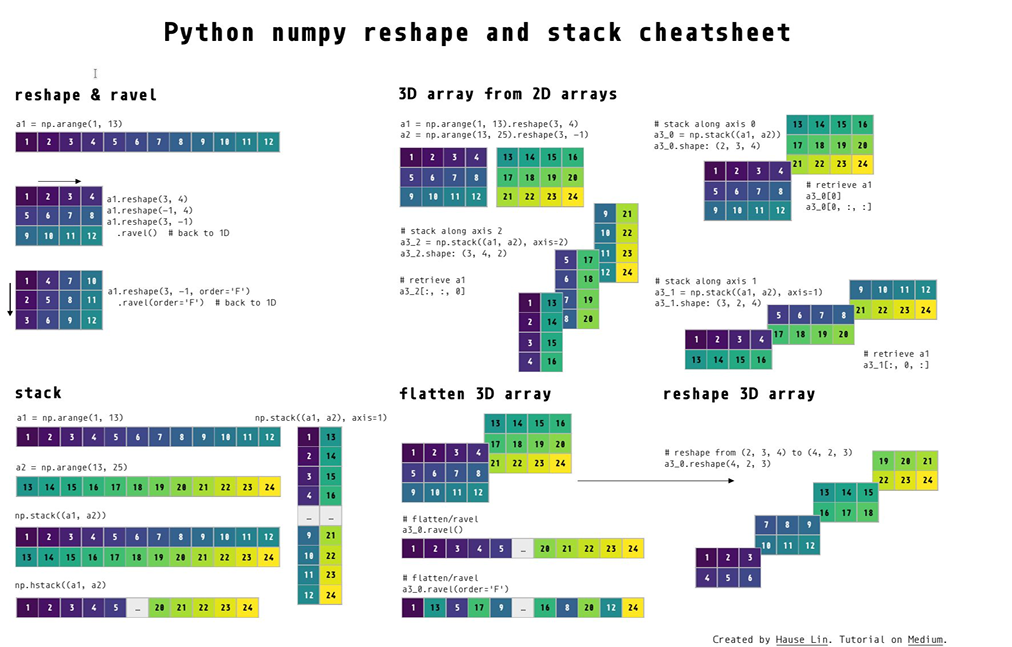
\includegraphics[width=\textwidth]{figuresML/lesson_ml_1_pag_999.png}
\end{center}

The first exercise consist of creating a simple classifier algorithm using an MLP and a DNN in order to compare their performances. In the second one you are required to build a regression algorithm by your own, so, even if the problem is already solved, you will find less guidelines and are encouraged to modify it and run it on your own. 

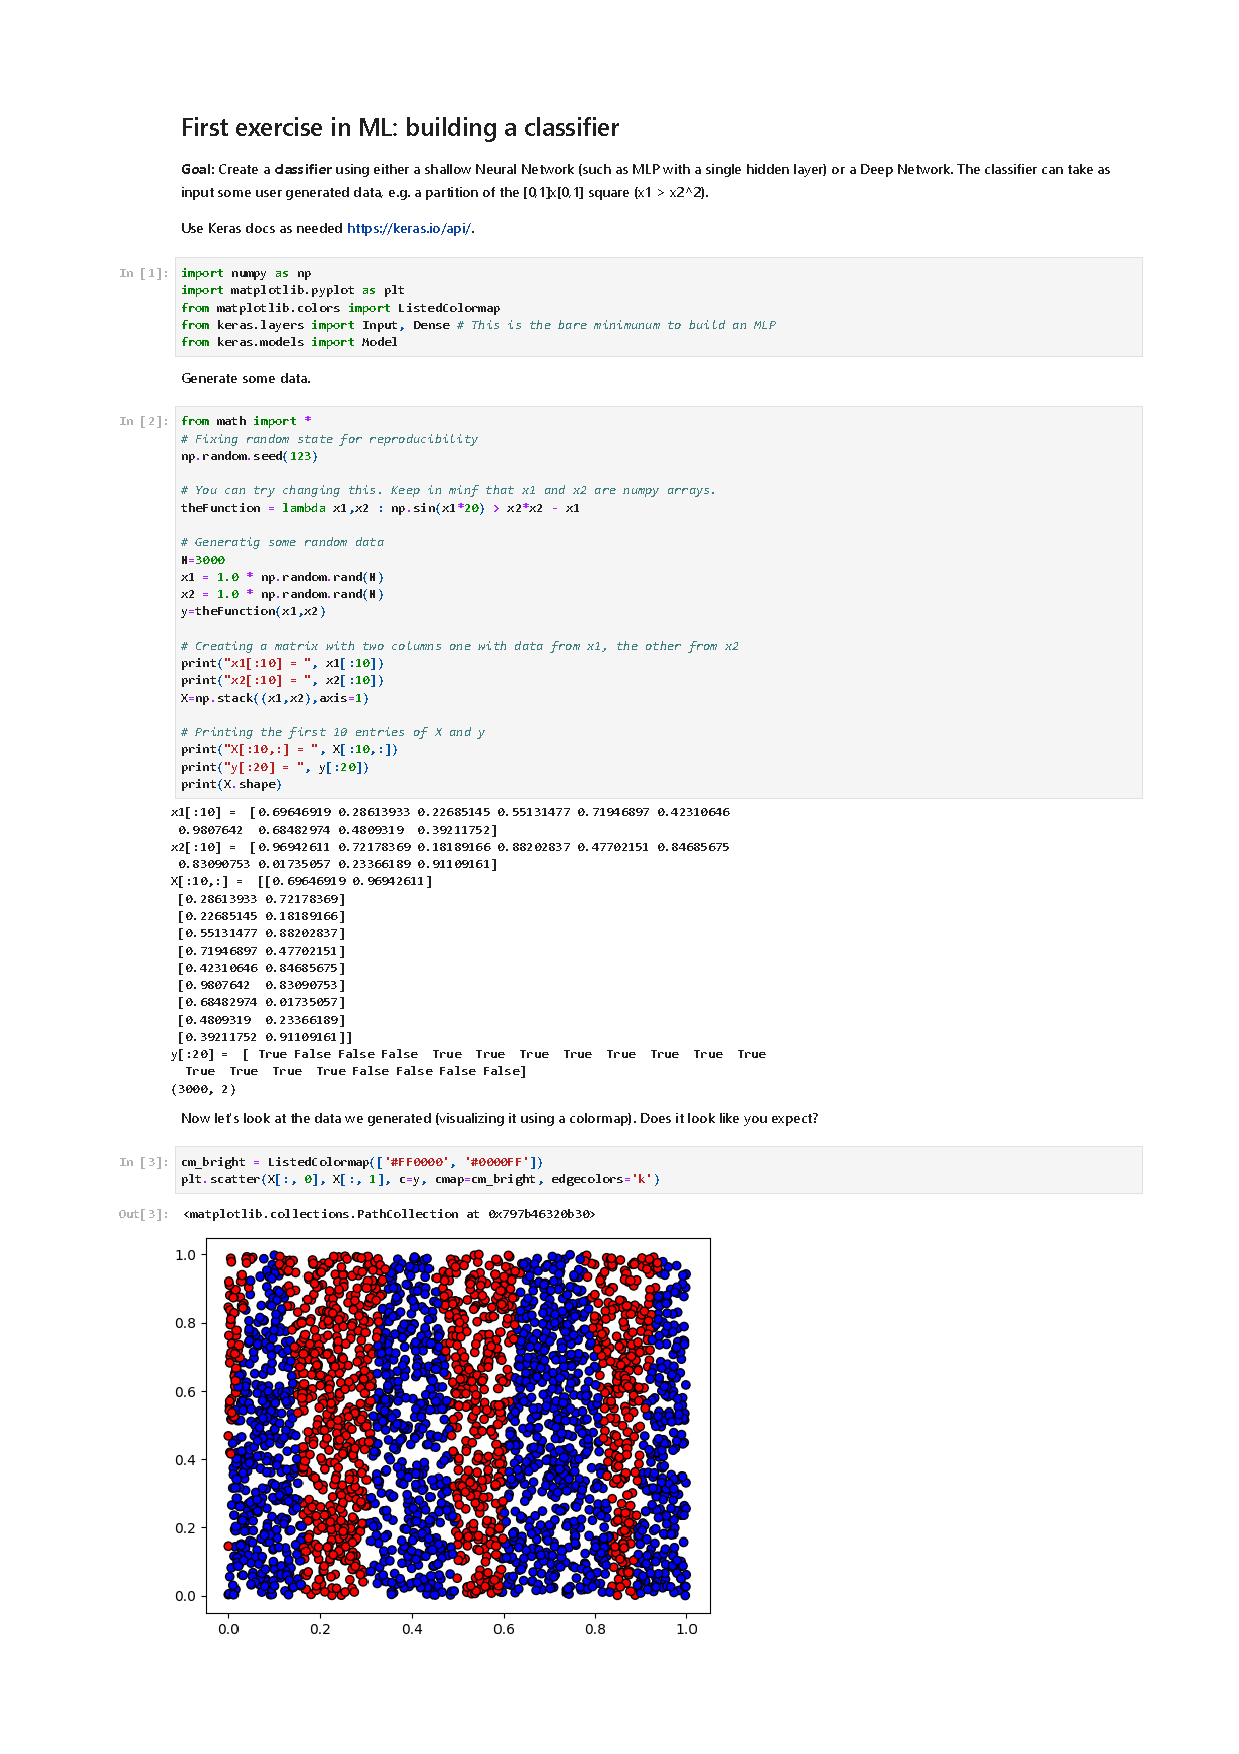
\includepdf[pages=-, pagecommand={\thispagestyle{plain}}]{lezioni/d_ML2A_SOL.pdf}

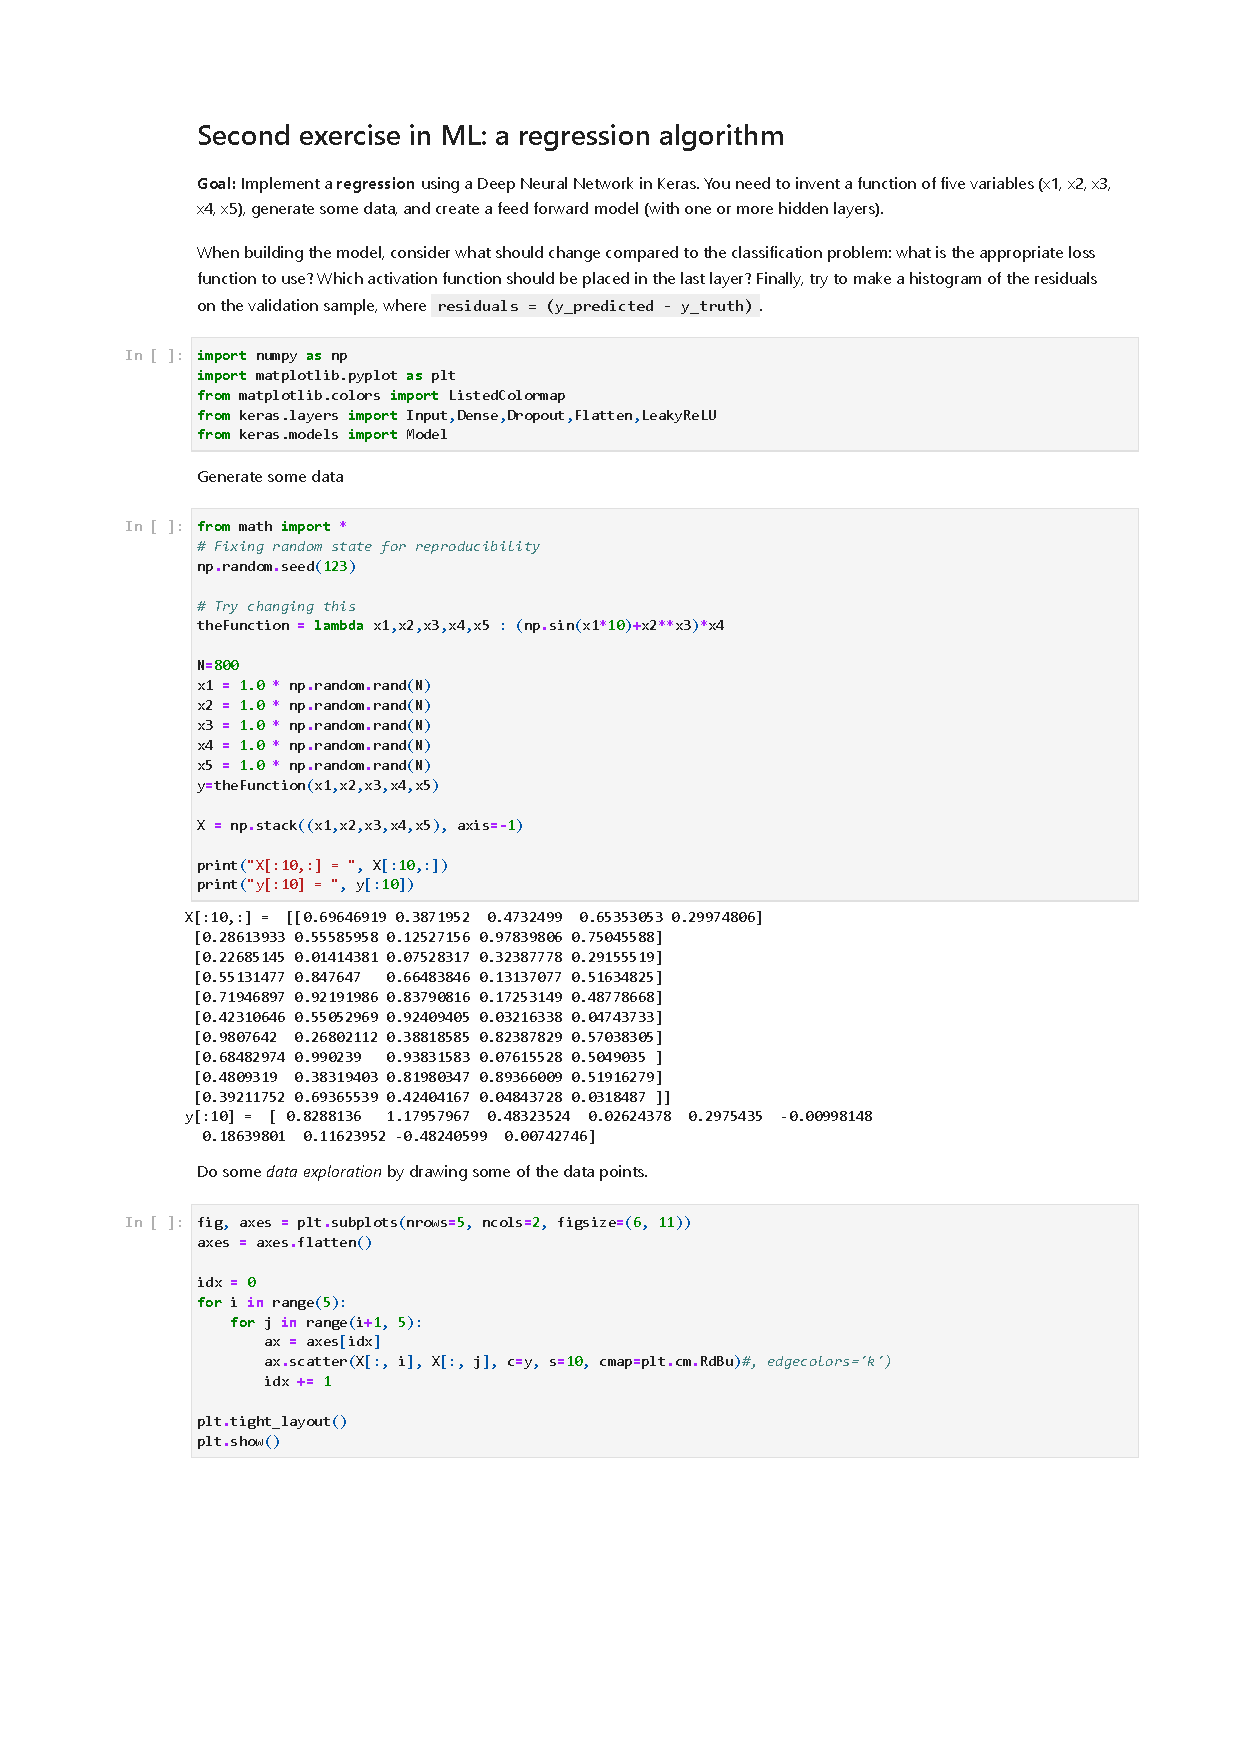
\includepdf[pages=-, pagecommand={\thispagestyle{plain}}]{lezioni/d_ML2B_SOL.pdf}

\section{Introduction to Convolutional Neural Networks and other architectures}

\subsection{Non-linearity: Universal Approximation Theorem}
As said, a NN is deep when it has many layers and it is wide if it has many neurons per layer. NNs are universal function approximators thanks to non-linearity. This concept can be expressed more rigorously through the so called \textbf{universal approximation theorem}: a feed forward neural network with:
\begin{itemize}
    \item[-] at least one hidden layer
    \item[-] a finite number of neurons
    \item[-] a non linear activation function (like sigmoid, ReLU, tanh)
\end{itemize}
can approximate \textit{any} continuous function on a compact subset of $\mathbb{R}^{n}$ to \textit{any} desired accuracy. We will not show a proof of this theorem but you can understand its importance: given enough neurons and the right weights, a neural network with even one hidden layer can model any continuous function on a compact subset as long as its activation function is not linear. Of course, the possibility of reaching a certain degree of accuracy in a reasonable amount of time strongly depends on the computational efficiency of our programs. 

With that said, here is a list of the many reasons why non-linear activation functions are required for a functional NN: 
\begin{enumerate}
    \item \textit{Linear layers alone are limited}: If a network only used linear transformations, stacking multiple layers would still represent a single linear function ($y = W_1(W_2 x) = (W_1 W_2)x$).
    \item \textit{Enable complex function approximation}: Real-world data involves highly non-linear patterns. Activations like ReLU, Sigmoid, or Tanh introduce this non-linearity allowing to approximate any continuous functions as stated by the universal approximation theorem.
    \item \textit{Class separation}: Problems like XOR cannot be solved by a linear classifier. Non-linear activation functions transform the input space so that classes become separable, as mentioned in the previous sections.
    \item \textit{Depth becomes useful}: Without non-linearity, adding more layers doesn't increase expressive power. With it, deeper networks can learn hierarchical features (edges $\rightarrow$ shapes $\rightarrow$ objects in vision tasks as we are going to see in a minute).
\end{enumerate}
After this brief discussion on non-linearity, we are going to move on towards convolutional neural networks. You might want to remember how an image is represented as a tensor, as mentioned in Sec. \ref{sec:ML_images}.

\subsection{Introduction to Convolutional Neural Networks (CNN)}
Since 2012, neural networks have gained ground for solving very complex problems due to many reasons, such as the massive amount of data available (thanks to Internet and research motors), hardware optimized for parallel computing (GPUs), software solutions for training (mainly in C since Python was still not optimized enough for the time), and theoretical maturity. In 2012, AlexNet, a convolutional neural network (CNN), won the ImageNet Large Scale Visual Recognition Competition (ILSVRC) by correctly classifying 83.6\% of the ImageNet dataset (about $1.3 \cdot 10^6$ images belonging to 1000 classes), marking the moment CNNs became the state of the art in Computer Vision. Starting from that date, the competition has always been won by CNNs. 

Before delving in the concept of CNN, let's define what a convolution is. A \textbf{convolution} is an operation between an $M \times N$ matrix $A$ (which in practice is our image and usually is squared with dimensions that are powers of 2 due to computational necessities) and a $k \times k$ (where $k$ is an odd integer) matrix $H$ called a \textbf{filter} or \textbf{kernel} defined as
\begin{equation}
C_{AH} = A \otimes H = \sum_{p=0}^{k-1} \sum_{q=0}^{k-1} A(i-p, j-q)H(p,q)
\end{equation}
The size of $H$ is called \textbf{receptive field}.

\begin{figure}[H]
    \begin{minipage}[c]{0.45\textwidth}
    Here is a visual representation of how a convolution between an input image and a $3 \times 3$ kernel works. Each element of the kernel represents a \textit{weight} and the result is called an \textbf{activation map}.
    \begin{enumerate}
        \item Superimpose the kernel to the first part of the image.
        \item Compute the product element wise between pixel and weights. That will become the first element of the activation map.
        \item "Slide" the kernel trough the image as shown and repeat the operations. Here we set the \textbf{stride} equal to 1 which means we will slide one pixel at a time, but for example we might not want overlapping pixels and set it to 4 instead.
    Notice that the activation map will be smaller than our input image. In particular its size can be easily computed as
    \begin{equation}
        M=\frac{N-k}{S}+1
    \end{equation}
    where $N$ is the image size, $k$ is the filter size and $S$ is the stride. \newline\newline 
    It should start to become clear that there is a big difference between using convolution and what we have done in the last sections, which was flattening all the data into a single vector. Such difference resides in the use of kernels, which let us work on a small part of our image at a time.  
    \end{enumerate}
    \end{minipage}\hfill 
    \begin{minipage}[c]{0.54\textwidth}
        \centering
        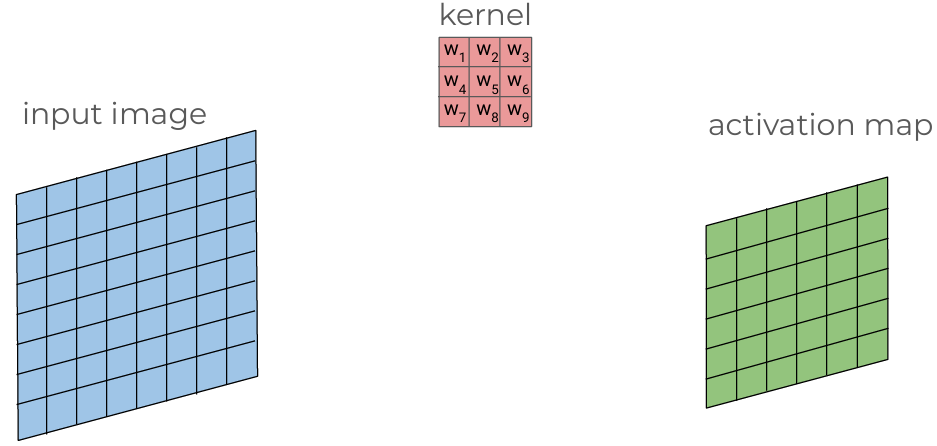
\includegraphics[width=0.8\linewidth]{figuresML/lesson_ml_3_pag_17.png}\hfill
        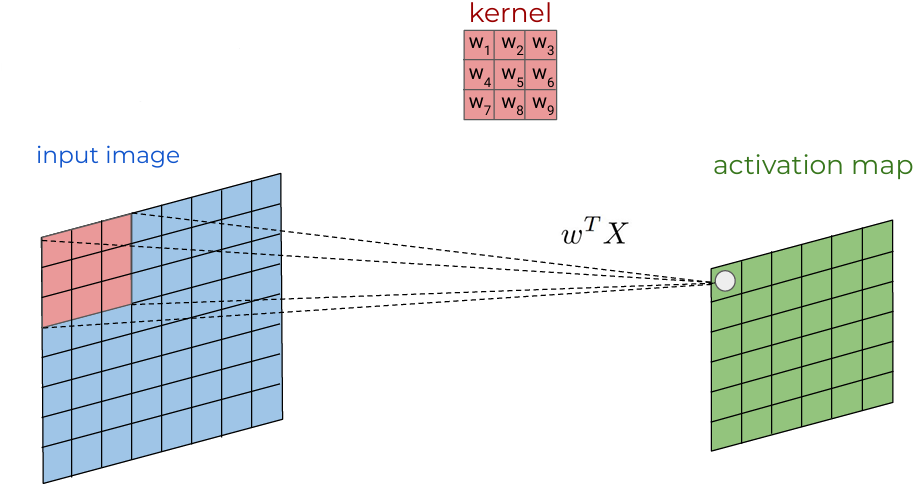
\includegraphics[width=0.8\linewidth]{figuresML/lesson_ml_3_pag_18.png} \\[.25cm] 
        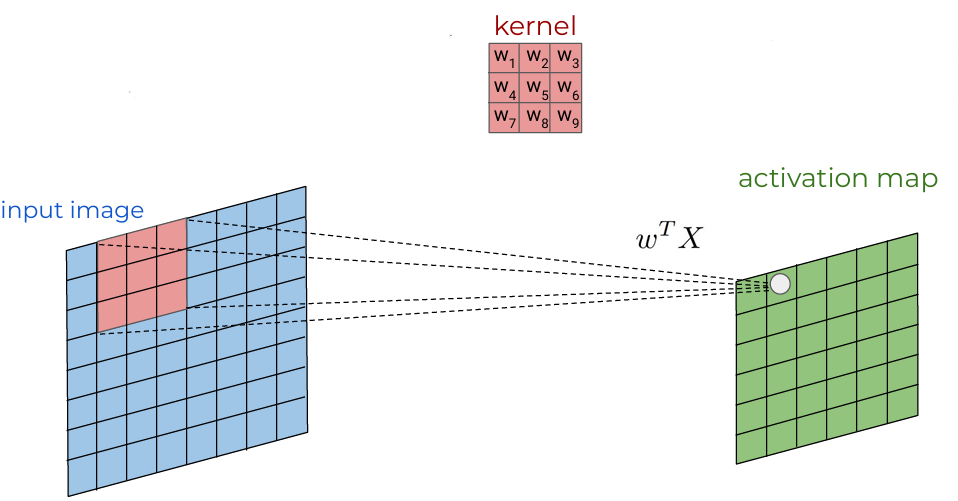
\includegraphics[width=0.8\linewidth]{figuresML/lesson_ml_3_pag_19.png}\hfill
        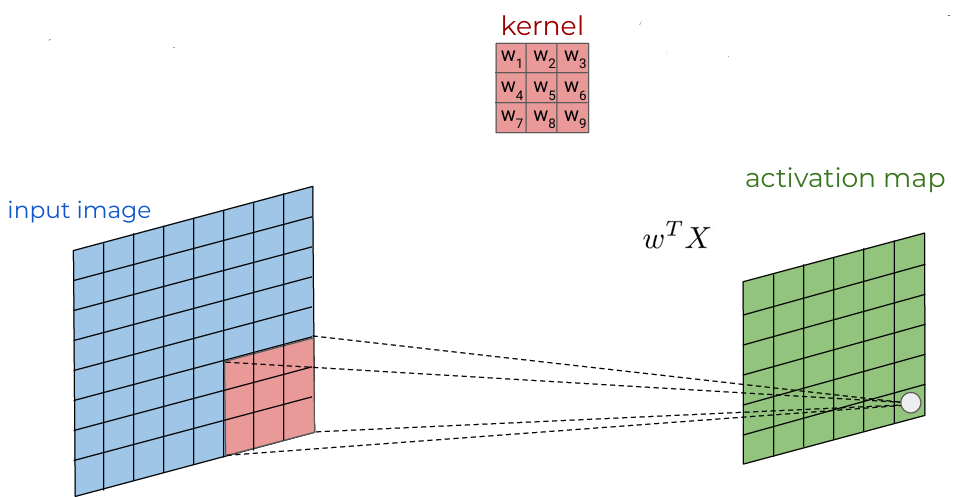
\includegraphics[width=0.8\linewidth]{figuresML/lesson_ml_3_pag_20.png}
    \end{minipage}
\end{figure} 
The idea of using a limited receptive field and of not connecting all the input pixels to all the neurons in the first layer comes from some biological hypothesis. In 1967, Hubel and Wiesel studied the response of the striate cortex in monkeys. They found that any small part of the striate cortex can be activated or suppressed in response to specific visual stimuli. So, animal vision is not performed by analysing each seen “pixel” but it works analyzing small part of the visual field. This led Fukushima in 1979 to invent the neocognitron, the first artificial neuron for vision.\\
We always use more than one kernel per layer (usually 32, 64, 128 and so on), and so we will have as many activation maps to work with. The figure below represents a typical convolutional layer, where each filter is learning a feature of the input image useful to solve our problem.
\begin{center}
    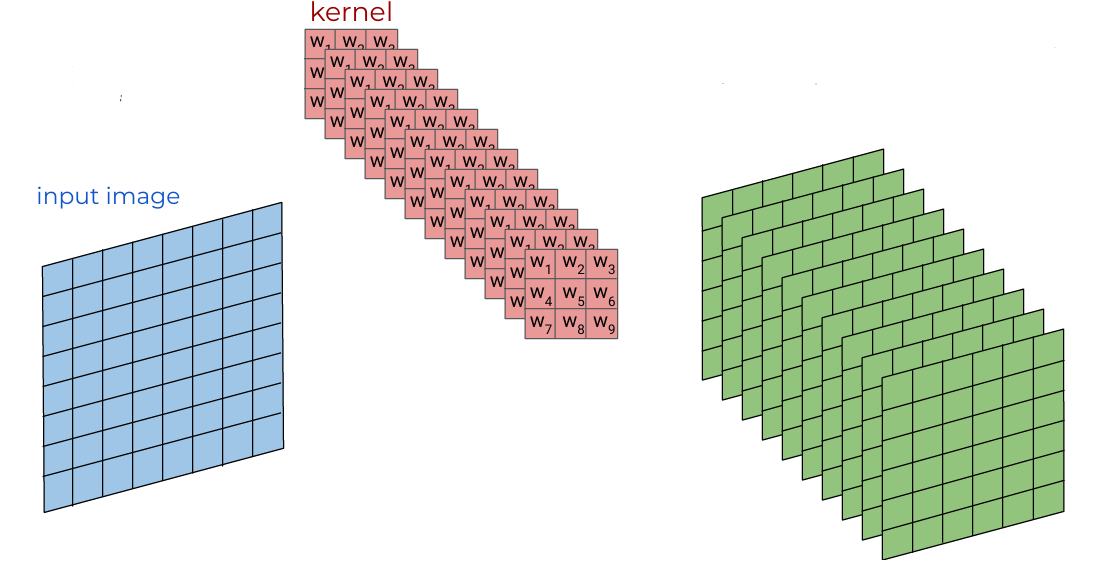
\includegraphics[width=0.6\linewidth]{figuresML/lesson_ml_3_pag_24.png}
\end{center}
Before the introduction of CNNs, the standard for computer vision was the so called \textit{feature engineering}, which is a method based on \textit{Sobel edge detection operators}. In practice these operators were kind of similar to filters, but their form was analytically defined a priori: finding filters, and hence features, capable of representing the information necessary to solve a complex problem (e.g classification of benign / malignant lesion in medical images etc...) was extremely complicated  and not as effective.

As you can see here, through the learning process, a CNN changes the value of the elements in the kernels to find the best representation of the data: it usually starts from simple features and then slowly learns the more complex ones (e.g. edges $\rightarrow$ textures $\rightarrow$ complex objects). It should be clear now that the \textbf{kernels themselves are the neurons of a CNN}, as they contain the trainable parameters.
\begin{center}
    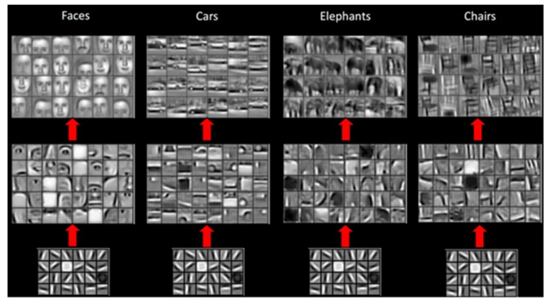
\includegraphics[width=0.6\linewidth]{figuresML/lesson_ml_3_pag_26.png}
\end{center}

Now that we understand the basics of CNNs we can ask ourselves \textit{why are CNNs so effective?} We can identify 3 main principles that make them so useful in the ML world:
\begin{enumerate}
    \item \textbf{Sparse connectivity:} Kernels slide over the image, meaning they connect only to a small, localized part of the input.
    \item \textbf{Sharing of parameters:} Through convolution, instead of learning a different set of parameters for each spatial position, the network learns only one set of weights per kernel. This induces... 
    \item \textbf{Translation invariance:} A feature is recognized regardless of its position in the image. For example, if a kernel is trained to recognize vertical lines, it doesn't matter where in the image the vertical lines is: thanks to parameter sharing and translation invariance it can be found wherever.
\end{enumerate}
Also, take a look at the following comparison: the number of parameters of a CNN is usually much smaller than the number of parameters of a classical NN with the same number of neurons.
\begin{center}
    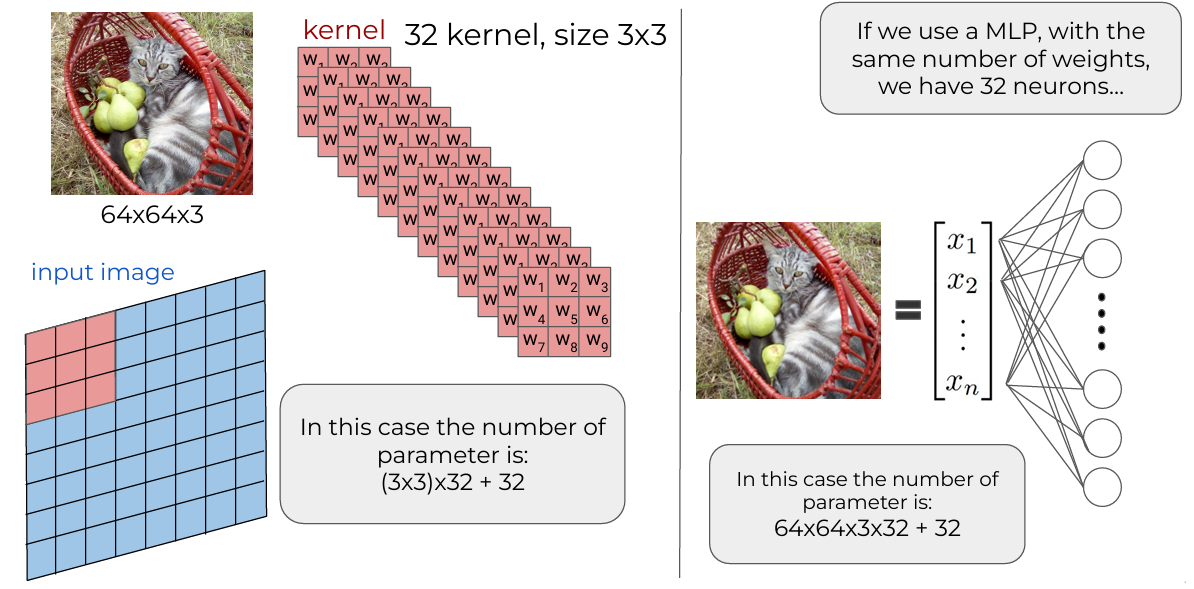
\includegraphics[width=0.75\linewidth]{figuresML/lesson_ml_3_pag_28.png}
\end{center}
\subsection{Structure of a Convolutional Neural Network}
As represented below, the typical structure of a CNN goes as follows:
\begin{itemize}
    \item[-] The input image is passed through:
    \begin{enumerate}
        \item A convolution operation;
        \item An activation function; 
        \item A pooling operation, which serves the purpose of compressing the information, drastically reducing the size of the activation maps (more information below).
    \end{enumerate}
    \item[-] All the operations are repeat layer after layer. 
    \item[-] The dimension of our data set is reduced step by step until we can flatten it and use a classifier algorithm like a NN.
\end{itemize}
\begin{center}
    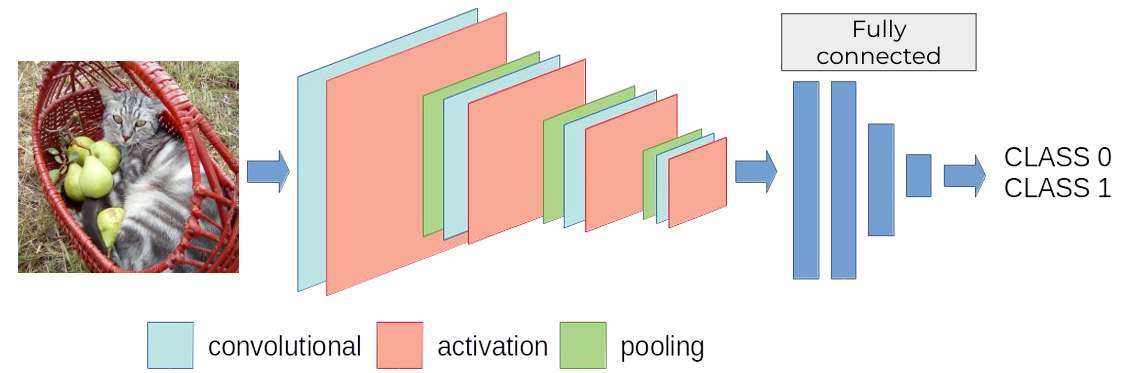
\includegraphics[width=0.8\linewidth]{figuresML/lesson_ml_3_pag_29.png}
\end{center}
Let's delve more deeply in the pooling process. \textbf{Pooling} is an invariant for permutation operation (such as a maximum or average) which is used, as said, to reduce the image / activation map size. As demonstrated below, applying a $2 \times 2$ max pooling operation with a stride of 2 involves extracting the maximum value from each non-overlapping $2 \times 2$ region of the input. The pooling window then shifts by two pixels (the stride) to evaluate the next block. Through this process, an initial $4 \times 4$ input tensor (or activation map) is downsampled into a compact $2 \times 2$ output tensor, effectively shrinking the size of the data while retaining the most prominent features.
\begin{center}
    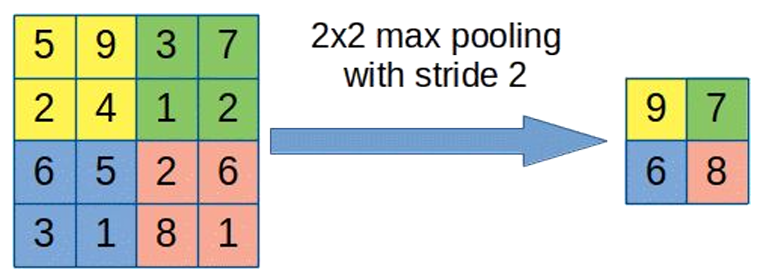
\includegraphics[width=0.35\linewidth]{figuresML/lesson_ml_3_pag_30.png}
\end{center}
Besides pooling, another method to reduce the size of the activation map and compress information is by increasing the stride of the convolution. As we have seen, the size of an activation map depends on the convolution parameters according to the formula:
\begin{equation*}
    M = \frac{N-k}{S} + 1
\end{equation*}
where $N$ is the image size (assuming an $N \times N$ image), $k$ is the filter/kernel size, and $S$ is the stride. What happens if we increase the stride? The resulting activation map becomes smaller. This introduces an alternative way to compress information, which raises an important question: is there a difference between using pooling and strided convolutions?

The key difference is that pooling does not add any parameters to the network; it is a fixed operation, meaning the network is not learning anything during this step and pooling just increases its efficiency. Conversely, a strided convolution relies on filters that contain trainable weights. In this case, we hope that the filters are not only learning to extract the necessary features to solve our task but are also simultaneously learning how to optimally compress the information. We cannot strictly control this behavior, as we simply rely on the optimization of the loss function. This highlights one of the main difficulties in developing neural networks: making numerous architectural choices (like whether to use a stride of 2, 3, or pooling instead) that can drastically change the model's performance.

Furthermore, we can "force" the convolution to slide over the entire image, including its edges, by using \textbf{padding}. Sometimes, we might want the output activation map to maintain the exact same spatial dimensions as the input (for instance, mapping a $64 \times 64$ input to a $64 \times 64$ output). Padding achieves this by adding extra pixels around the original image, allowing the kernel to start its convolution precisely on the boundaries, as shown below. The most common approach is zero-padding, but this can introduce strange artificial effects on the edges. Alternatively, one could pad using the average value of the overall image or the values of the corners. If the information at the edges of the image is crucial for the task, padding must be implemented carefully. Ultimately, this means there are many hyperparameters and design choices that must be fixed even within a single convolutional layer.

\begin{center}
    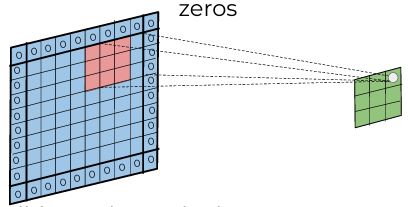
\includegraphics[width=0.35\linewidth]{figuresML/lesson_ml_3_pag_33.png}
\end{center}

We also mentioned that towards the end the input tensors can be flattened and fed into a classifier like a NN. We can do so in many ways, but the easier one would be to flatten the last activation $n \times m$ activation maps. The input of our classifier would then be a vector with length equal to  $n \times m \times a$ where  $a$ is the number of activation maps. This number can be too large with respect to the weights of the entire 
network. For example, if the last convolutional layer has 128 activation maps ($\rightarrow$ 128 kernels) with size $16 \times 16$ and the classifier is a fully connected NN with 100 neurons in the first layer, the number of parameters that are induced is $128 \times 16 \times 16 \times 100 = 3.276.800$. This problem is nearly always relevant due to the fact that \textit{it is convenient to choose a large number of small kernels in order to describe complex features} (we will say some more about this concept in a while). 

Instead, we could use \textbf{aggregation functions} in order to combine the data in the activation functions. The most common aggregation function is the \textbf{Global Average Pooling} (GAP), which consists in simply computing the average of each activation map (so each one is collapsed into a single number) and then vectorizing the result. In the previous example, the number of parameters is reduced to $128 \times 100 = 12.800$ (number of activation maps times number of neurons in the first layer of the NN).

Finally, if the last classifier is a NN, \textit{we can train the entire structure end-to-end}, as seen in previous chapters, by defining a loss function, applying backpropagation, and optimizing the parameters. This has some advantages, like a better accuracy for kernel parameters. However, we can also use the CNN strictly as a \textbf{feature extractor}, i.e. an instrument that translates a complex input image in a simple numerical vector. In this case, the output from the flattening, can be used directly as input features to feed a completely different machine learning algorithm, such as a Decision Tree. We will explore this approach later when discussing Transfer Learning.

\subsection{Evolution of CNN Architectures}

The easiest way to improve a CNN algorithm is finding a way to extract and comprehend more precisely and efficiently, for example by building deeper and deeper networks. However, this requires hardware able to withstand an enormous amount of computation: not every problem can be solved by a bigger GPU, and one of the most important factors of progress in the ML world is also finding ways to reduce the computational cost of training. These are the two main research goals in the field.

With said, let's briefly review the recent history and improvements of CNNs by looking at some of the most important examples of CNNs:

\begin{center}
    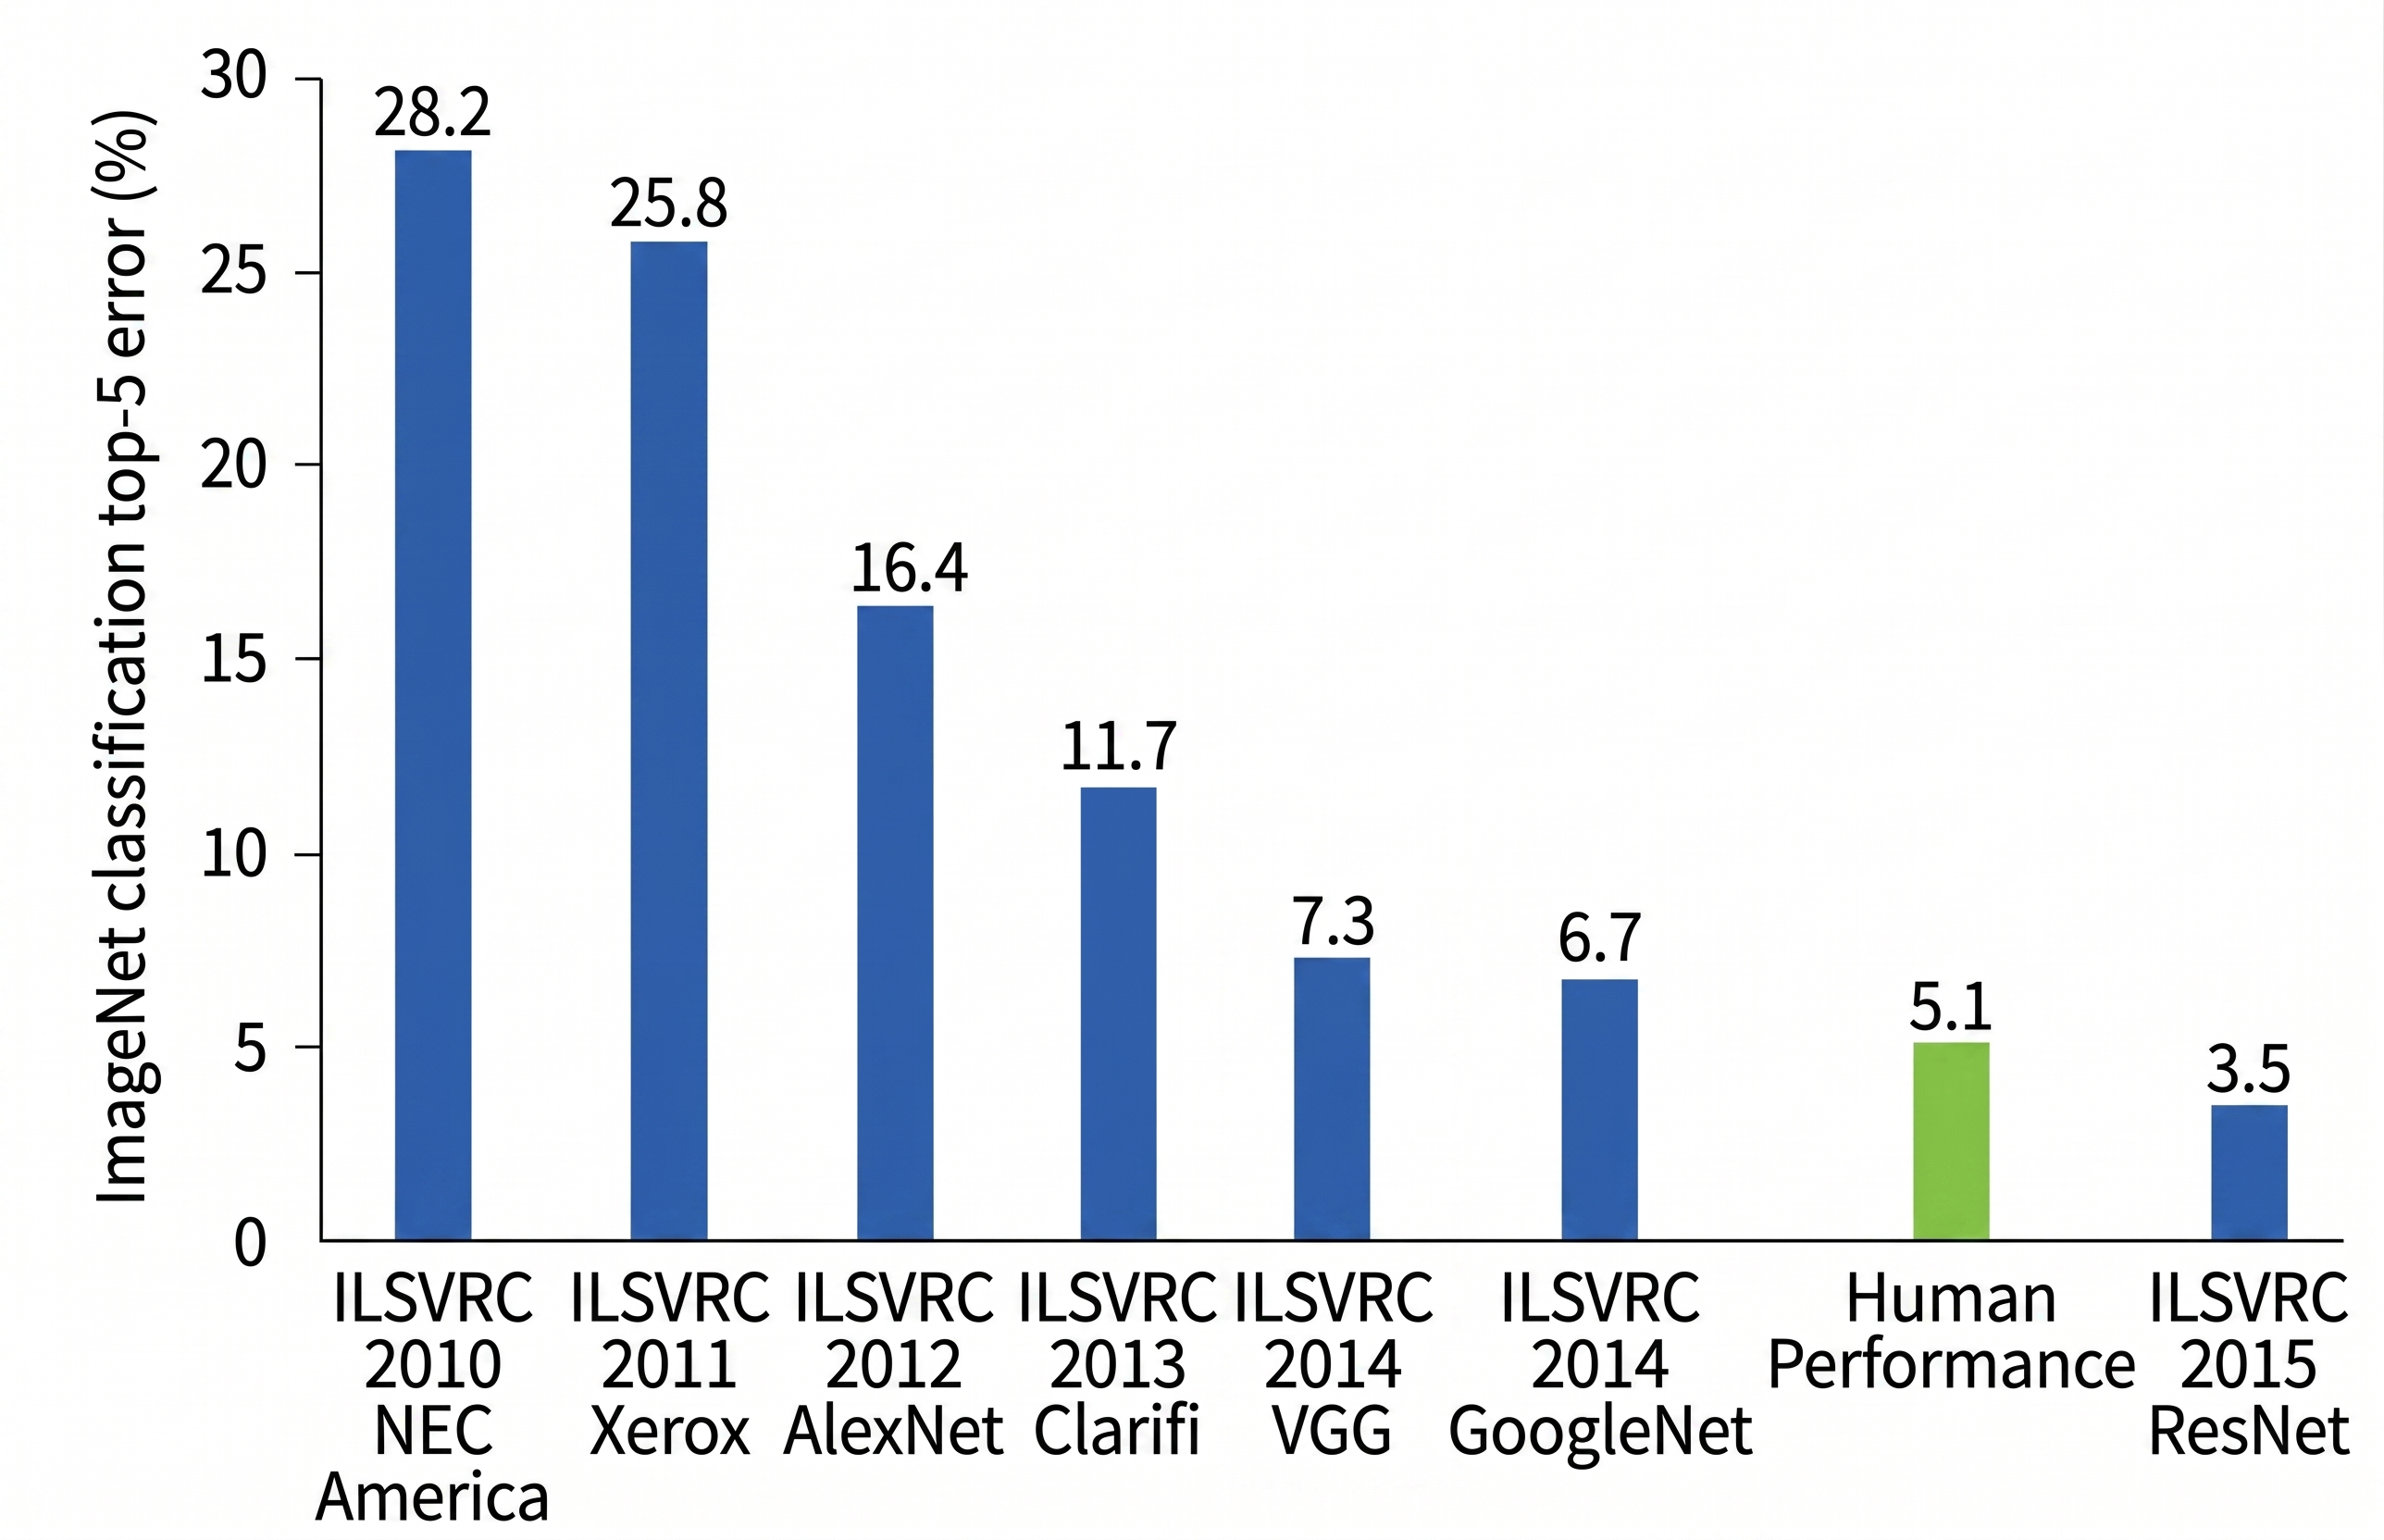
\includegraphics[width=0.45\linewidth]{figuresML/lesson_ml_3_pag_46.png}
\end{center}

\textbf{- AlexNet (2012):} Created by Alex Krizhevsky et al., AlexNet had 8 convolutional layers and outperformed all competitors in the ILAVRC by combining a series of previous revolutionary work with important innovations like:
\begin{itemize}
    \item[-] The neocognitron, proposed by Kunihiko Fukushima in 1979;
    \item[-] A backpropagation algorithm, a term coined by Rosenblatt in 1962 and which evolved greatly between the 1970s and the early 2000s;
    \item[-] LeNet, proposed by Yan LeCunn in 1998;
    \item[-] GPU acceleration first proposed by Kumar Chellapilla;
    \item[-] A new (for the time) activation function: the ReLU;
    \item[-] Data augmentation and many other "small" adjustments;
\end{itemize}

\textbf{VGG19 (2014):} In 2014, a network called VGG19 with 19 layers by Karen Simonyan and Andrew Zisserman won the ImageNet competition. The main difference that led them to improve the design of AlexNet by being able to add more layers is a clever implementation of the pooling system. AlexNet: contemplates the use of convolution filters of different sizes, from largest to smallest: $11 \times 11$, $5 \times 5$, $3 \times 3$ and then $3 \times 3$ throughout the architecture. With this structure, the number of parameters for the $11 \times 11$ layer is $11 \times 11 \times 32 = 3872$ where 32 is the number of filters. Istead of using “large” filters ($11 \times 11$ or $5 \times 5$), VGG19 uses small ones sequentially before pooling. Five $3 \times 3$ filters in sequence have an \textbf{effective receptive field} of $11 \times 11$ with a smaller number of parameters: $3 \times 3 \times 32 \times 5 = 1440$ where 32 is the number of filters and 5 the number of layers. It is therefore possible to go deeper by reducing the number of learnable (trainable) parameters. 

What exactly do we mean with effective receptive field? The effective receptive field is the spatial extent of the original input image that contributes to the calculation of a single pixel in a given activation map. As illustrated in the comparison below, a single $5 \times 5$ convolution directly looks at a $5 \times 5$ area of the input. However, if we stack two $3 \times 3$ convolutional layers, the first layer processes $3 \times 3$ regions, and the second layer processes $3 \times 3$ regions of those intermediate activations. Ultimately, a single pixel in the output of the second layer implicitly depends on a $5 \times 5$ region of the original input. 

Both approaches "look" for correlations at the exact same points in the input image, maintaining an effective receptive field of $5 \times 5$. The critical advantage lies in parameter efficiency: assuming 32 channels, a single $5 \times 5$ layer requires $5 \times 5 \times 32 = 800$ parameters. In contrast, the two stacked $3 \times 3$ filters require only $3 \times 3 \times 32 \times 2 = 576$ parameters. This principle allowed VGG19 to stack many more layers, increasing the non-linearity and depth of the network while keeping the computational cost manageable.

\begin{center}
    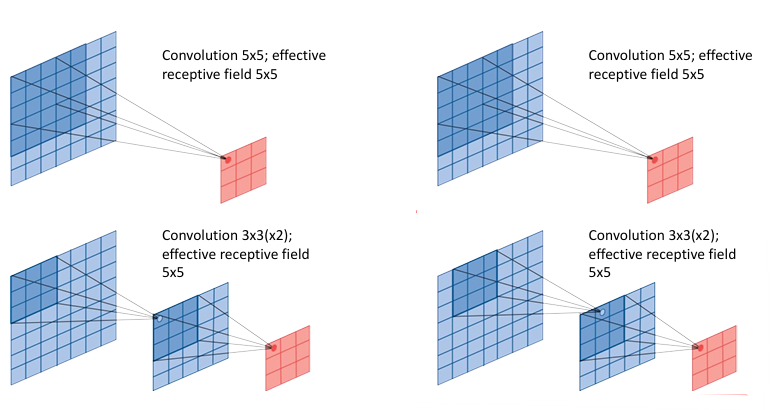
\includegraphics[width=0.7\linewidth]{figuresML/lesson_ml_3_pag_49.png}
\end{center}

\textbf{InceptionLeNet (2014):} In 2014 the InceptionNet 22 layers CNN won the ImageNet competition. It implemented an architecture that was used to search for representations at multiple scales: the input (or simply the output of the previews layer) was passed through multiple \textit{parallel} layers with filters of different sizes and then the filters output was concatenated with various techniques, as represented here.

\begin{center}
    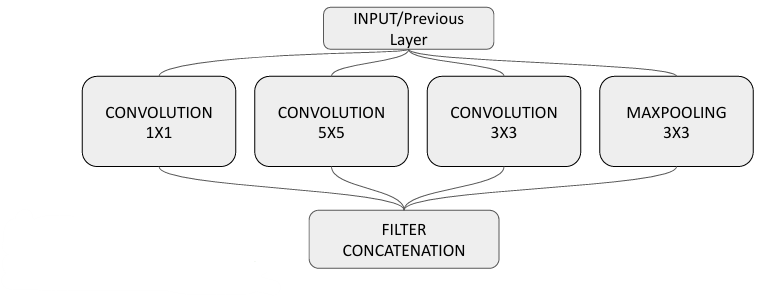
\includegraphics[width=0.6\textwidth]{figuresML/lesson_ml_3_pag_54.png}
\end{center}

This method, however, has a serious problem: the number of parameters explodes. In this naive configuration, applying multiple parallel filters (such as $1 \times 1$, $3 \times 3$, and $5 \times 5$ convolutions) directly to an input with a high number of channels results in a massive computational cost. For example, even with a relatively small input depth and a limited number of filters per convolution, the parameter count quickly skyrockets. To solve this, the so called \textbf{inception block} introduces a clever workaround: it adds $1 \times 1$ convolutions before the more expensive $3 \times 3$ and $5 \times 5$ convolutions, as well as after the max pooling layer. These $1 \times 1$ convolutions serve to reduce the depth of the input data (i.e., the number of channels from the previous block). 
For example, consider an input with 256 channels and a target of 32 output filters using a $5 \times 5$ convolution:
\begin{itemize}
    \item \textit{Naive approach:} A direct $5 \times 5$ convolution requires $5 \times 5 \times 256 \times 32 = 204,800$ parameters.
    \item \textit{Inception approach:} Using a $1 \times 1$ convolution to first reduce the input depth (as shown below) to 16 channels requires $(1 \times 1 \times 256 \times 16) + (5 \times 5 \times 16 \times 32) = 4,096 + 12,800 = 16,896$ parameters. 
\end{itemize}
This simple bottleneck step eliminates over 90\% of the computational cost. By shrinking the dimensional depth before applying larger kernels, InceptionNet drastically reduces the total number of trainable parameters, making the architecture computationally viable while still successfully capturing multi-scale representations.

\begin{center}
    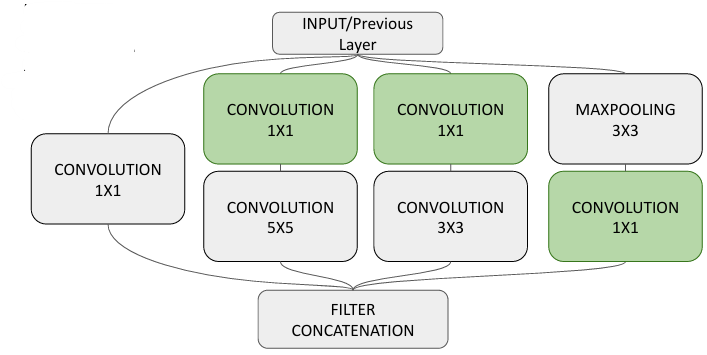
\includegraphics[width=0.5\textwidth]{figuresML/lesson_ml_3_pag_57.png}
\end{center}

\begin{figure}[H]
    \begin{minipage}[c]{0.54\textwidth}
    Here is a figure taken from the original InceptionNet paper. As you can see the input data is processed through the other convolutional layers before entering the inception block. This ensures that the size of the data at the input of the inception block is $a \times b \times F$ where $F$ of filters of the previous layer and $a \times b$ is the size of the previous activation function. \newline \newline
    \textbf{ResNet(2015)}: A massive jump in depth was achieved by the ResNet CNN, which featured 152 layers and exceeded the human capabilities in the classification task of the ImageNet competition. As we already mentioned hundreds of times, as the number of layers increases, the number of neurons increases and so does the number of trainable parameters. Note that when the computational cost becomes higher and higher, not only you are going to need for higher performance GPUs (in particular VRAM), but you will also face simple logistics problem during development: if the algorithm you want to train takes 2 weeks to run, it will be more complicated to develop since you will be able to debug it only twice a month!
    \end{minipage}\hfill 
    \begin{minipage}[c]{0.45\textwidth}
        \centering
        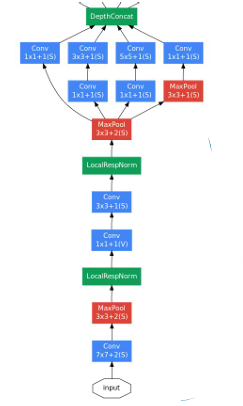
\includegraphics[width=0.8\linewidth]{figuresML/lesson_ml_3_pag_58.png}\hfill
    \end{minipage}
\end{figure} 

\subsection{The vanishing gradient problem}\label{sec:skip_connections}

There is another problem specific to CNNs (but also true for NN): the nightmare of the vanishing gradient. As said, training a CNN means using backpropagation to update the weights once the loss function has been calculated and it requires the calculation of many derivatives. Close to convergence, when the neural network is close to a local minimum of the cost function, the variations in the weights will become very small, which means the derivatives of the loss with respect to this small changes will be very small, close to 0. Applying the chain rule for calculating the gradient simply means that, to update the weights of the neural network, we must multiply many of these derivatives. Multiplying many small factors leads to gradients approaching zero and that is the so called \textbf{vanishing gradient problem}. 

Such problem has many causes, for example a wrongful choice for the activation function. If you look at a sigmoid, it is easy to see that as $x$ increases, the derivative of the function goes to zero, which does not happen for the ReLu. However, the fact that for negative values the ReLu is zero can cause some problems, easily manageable by changing the activation function to a Leaky ReLu or some other variant. 

Wrongful weight initialization can also cause the same problem. Consider the following example.
\begin{center}
    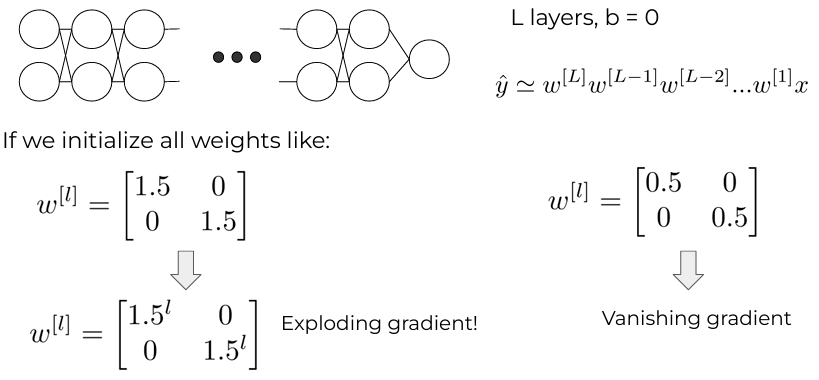
\includegraphics[width=0.6\textwidth]{figuresML/lesson_ml_3_pag_71.png}
\end{center}
Given the $L$ layers of the DNN, if we initialize all weights with values smaller than 1 (for example, $0.5$), repeated multiplications across the layers during backpropagation will result in terms proportional to $0.5^L$. For deep networks, this value quickly approaches zero, causing the vanishing gradient. Conversely, initializing weights with values strictly greater than 1 (like $1.5$) will result in terms proportional to $1.5^L$, which rapidly grow out of control and lead to an exploding gradient.

There are many ways to correctly initialize weights that have been proven to work in an empirical way. Given the complexities of DL algorithms, it should not come as a surprise that sometimes we just need to rely on practice to make something work even if we cannot comprehend \textit{why} it works a priori. Here are some examples:
\begin{itemize}
    \item[-] \textit{Random initialization}: sampling the weights from a normal distribution or a uniform distribution, usually independently.
    \item[-] \textit{LeCun initialization}: it is designed to preserve the variance of neural activations during the forward pass. It samples each entry $W(l)$ independently from a distribution with mean 0 and variance $1/n_{l-1}$.
    \item[-] \textit{Glorot initialization}: it preserves activation variance during the forward pass and gradient variance during the backward pass.
    \item[-] \textit{He initialization}: Since Glorot initialization performs poorly with ReLU, we can use
    \begin{equation*}
        w^{[l]}=\sqrt{\frac{2}{n^l + n^{(l-1)}}}
    \end{equation*}
\end{itemize}

Lack of \textit{batch normalization} can also lead to a vanishing gradient.It consists in the normalization of the inputs of each layer so that they have a stable distribution during training. It is typically applied after the convolutional layer and before the activation function (like ReLU), calculating $\hat{x} = \frac{x - \mu}{\sqrt{\sigma^2 + \epsilon}}$ computed on a batch of data. It was introduced to address the problem of \textbf{internal covariate shift}:
\begin{itemize}
    \item[-] When weights in earlier layers change, the outputs of those layers also change.
    \item[-] These outputs become the inputs for the next layer, so their statistical properties (mean, variance) shift.
    \item[-] This forces subsequent layers to constantly adapt to new input distributions, making training harder.
\end{itemize}
Without this normalization step, the network suffers from slower training, requires smaller learning rates, and becomes highly susceptible to exploding or vanishing gradients.

Lastly, we said that as we try to build deeper networks, the number of multiplications required to compute derivatives during backpropagation increases significantly and if these individual derivatives are close to zero, multiplying many of them together inevitably leads to the vanishing gradient problem. To solve this, we must find a way to decrease the number of multiplications required for the gradient. The solution comes in the form of \textbf{residual skip connections}, which are connections bridging non-adjacent layers, as shown in figure. This mechanism is the foundational idea behind the ResNet architecture.

\begin{center}
    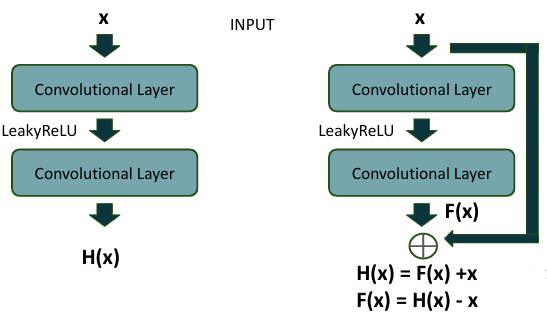
\includegraphics[width=0.5\textwidth]{figuresML/lesson_ml_3_pag_78.png}
\end{center}

Instead of forcing the network to learn a direct mapping entirely through stacked convolutional layers, skip connections introduce an identity mapping. If the output of a block of convolutional layers is $F(x)$ and the original input to that block is $x$, the skip connection directly adds the input to the output. This results in the final mapping is $H(x) = F(x) + x$. \\ 
This simple addition has a profound mathematical impact during backpropagation: when computing the gradient with respect to $x$, the derivative becomes $\frac{\partial F}{\partial x} + 1$. The addition of the $+1$ ensures that even if $\frac{\partial F}{\partial x}$ becomes infinitesimally small, the overall gradient will not vanish. 
Implementing skip connections provides several key advantages:
\begin{itemize}
    \item[-] Enables deeper networks.
    \item[-] Mitigates the vanishing gradient.
    \item[-] Improves convergence speed (the network learns faster because the gradient has shorter, direct paths to earlier layers).
    \item[-] Preserves fine details (original input information bypasses intermediate transformations, maintaining fine-grained details better throughout the network).
\end{itemize}

\subsection{Notes on explainability and transfer learning}

CNNs dramatically changed the trajectory of Neural Networks and AI. Their success in computer vision proved that deep architectures could outperform traditional methods, which fueled massive interest and investment in deep learning. This breakthrough laid the foundation for subsequent advances, including architectures like transformers that power models such as GPT. After the 2017 edition, the ImageNet competition was officially closed and today it remains one of the totems of the massive progress the field experience during the 2010s. Today Convolutional Neural Networks are still very powerful models but as any other deep learning algorithm they can be considered black boxes: this simply means that we cannot fully understand why they take certain decisions as we may have million of million of trainable parameters. There is an entire branch of AI research called eXplainable AI (XAI) that aim to develop method to explain NN. One of the most used method for CNN is called \textit{gradCAM} which exploits the global average pooling (we will not be focusing on this, you can research it on your own if interested).

Another fundamental concept in modern Deep Learning is \textbf{transfer learning}. In many real-world scenarios, we might want to leverage the power of a complex CNN, but we simply do not have enough data to train such a massive algorithm from scratch. To overcome this limitation, we can exploit the structural composition of a CNN, which (as we saw before) is essentially divided into two main components: the \textbf{convolutional part} (which acts as a \textit{feature extractor}) and the \textbf{classifier} (typically a fully connected NN or MLP). By training the entire network on a very large, generalized dataset first, we can reuse it for our specific, smaller dataset using two main strategies:
\begin{itemize}
    \item[-] \textbf{Feature Extraction:} We split the network and use only the first part. The pre-trained convolutional layers extract the features from our new data, and this output (after a flattening or global average pooling step) is then used as the input for a new, independent classifier. \\ Example: Using a CNN pre-trained on ImageNet (millions of general images) to extract basic shapes and textures, and training only a new, simple classifier on top to recognize specific flower species.
    \item[-] \textbf{Fine Tuning:} We take the pre-trained network, change a small portion of the architecture, and train the whole system again to fit our specific data. Common modifications include adapting the input (e.g., adjusting to smaller/bigger images, or switching between grayscale and RGB) or modifying the output (e.g., replacing the final layer of a network originally trained for 100 classes so that it can perform a simple binary classification). \\ Example: Taking an ImageNet model, replacing its 1000-class output layer with a 2-class layer, and gently re-training the entire network to adapt its filters for detecting tumors in medical X-rays.
\end{itemize}

\section{Regularization, bias and variance more in depth}

\subsection{A brief review}
Let's review some useful concepts from the previous sections. \\
Different machine learning techniques with specific sets of hyper-parameters) can represent different types of functions. Generally, a model with more free parameters can approximate a larger number of functions. This ability to represent many functions is referred to as the model \textit{capacity}, which basically represents the model ability to use information effectively. In the context of a Neural Network, adding more neurons (making it wider) or more layers (making it deeper) directly translates to a greater capacity. Remember also that our goal is not simply to fit the training data perfectly, but to ensure that the algorithm works well on unseen data, which means it has to have a good \textit{generalization capability}. if a model has too low of a capacity for the complexity of the data, it will fail to capture the underlying trend, resulting in \textit{underfitting}. Conversely, if the capacity is too high, the model will memorize the noise in the training set rather than the actual signal, leading to \textit{overfitting}. The difference between the training error and the generalization error is known as the \textit{generalization gap}. To achieve good performance on unseen data even when utilizing a high number of parameters, we must rely on \textit{regularization techniques}. The cost function can be modified by introducing a penalty term to limit certain parts of the model-parameter space, or we can use techniques like data augmentation, adding stochastic noise, or applying invariant transformations.

\subsection{Bias vs Variance: a formal derivation for regression}

Generalization and capacity are deeply connected, and finding the right balance is one of the core challenges in Machine Learning. To better understand this kind of tradeoff, we will lay out a formal mathematical demonstration in the case of regression.

Let us consider a training dataset $S = \{x^{(i)}, y^{(i)}\}_{i=1}^n$ such that the true relationship is given by:
\begin{equation}
    y^{(i)} = h^*(x^{(i)}) + \xi^{(i)}
\end{equation}
where $h^*$ is the true underlying function and $\xi^{(i)}$ is an intrinsic noise term drawn from a normal distribution $\mathcal{N}(0, \sigma^2)$. We want to train a regression model, denoted as $\hat{h}_S$, on this dataset $S$.

When we evaluate this model on a new, unseen test sample $(x, y)$ (where $y = h^*(x) + \xi$ with $\xi \in \mathcal{N}(0, \sigma^2)$) we measure the expected test error using the mean squared error:
\begin{equation}
    MSE(x) = \mathbb{E}_{S,\xi}\left[(y - \hat{h}_S(x))^2\right]
\end{equation}
We can decompose this term into \textit{variance} and \textit{bias} by using a known property of expected values: if $A$ and $B$ are two independent real random variables and $\mathbb{E}[A]=0$, then $\mathbb{E}[(A+B)^2] = \mathbb{E}[A^2] + \mathbb{E}[B^2]$. As a corollary, if $B$ is a constant $c$, then $\mathbb{E}[(A+c)^2] = \mathbb{E}[A^2] + c^2$. Applying this claim with $A = \xi$ and $B = h^*(x) - \hat{h}_S(x)$, we obtain:
\begin{equation}
    MSE(x) = \mathbb{E}_{S,\xi}\left[ \left(\xi + (h^*(x) - \hat{h}_S(x))\right)^2 \right] = \mathbb{E}[\xi^2] + \mathbb{E}_S\left[(h^*(x) - \hat{h}_S(x))^2\right]
\end{equation}
Since the expected value of the squared noise $\mathbb{E}[\xi^2]$ is simply its variance $\sigma^2$, the equation simplifies to:
\begin{equation}
    MSE(x) = \sigma^2 + \mathbb{E}_S\left[(h^*(x) - \hat{h}_S(x))^2\right]
\end{equation}
Now, let us define an "average model" $h_{avg}(x) = \mathbb{E}_S[\hat{h}_S(x)]$. This represents an ideal model obtained by drawing an infinite number of datasets, training on all of them, and averaging their predictions (for many cases, it corresponds to one single model trained on infinite samples). By adding and subtracting $h_{avg}(x)$ inside the expectation, we can further decompose the MSE by letting $c = h^*(x) - h_{avg}(x)$ (which is a constant with respect to $S$) and $A = h_{avg}(x) - \hat{h}_S(x)$:
\begin{equation}
    MSE(x) = \sigma^2 + (h^*(x) - h_{avg}(x))^2 + \mathbb{E}_S\left[(h_{avg}(x) - \hat{h}_S(x))^2\right]
\end{equation}
This final equation highlights the three fundamental components of the generalization error:
\begin{equation}
    MSE(x) = \sigma^2 + \text{Bias}^2 + \text{Variance}
\end{equation}
where:
\begin{itemize}
    \item[-] $\sigma^2$ is the irreducible error, caused by the inherent randomness in the dataset.
    \item[-] The \textbf{bias} squared $(h^*(x) - h_{avg}(x))^2$ represents the lack of expressivity of the model. It shows the error introduced because the chosen model cannot represent the true data distribution, not due to a lack of data.
    \item[-] The \textbf{variance} $var(\hat{h}_S(x))$ quantifies how the random nature of the finite dataset introduces error in the model's predictions.
\end{itemize}

\begin{figure}[H]
    \begin{minipage}[c]{0.6\textwidth}
        Bias tends to decrease when the model becomes more complex, while variance shows the opposite behavior, as shown here. As you might imagine is never easy to reach the sweet spot between the two. \\ The concepts of capacity, generalization, bias, and variance are strictly intertwined. A model's capacity dictates its position on the bias-variance tradeoff: low-capacity models lack the expressivity to capture the true function, leading to high bias (underfitting), while high-capacity models tend to memorize the training noise, resulting in high variance (overfitting).
    \end{minipage}\hfill 
    \begin{minipage}[c]{0.39\textwidth}
        \centering
        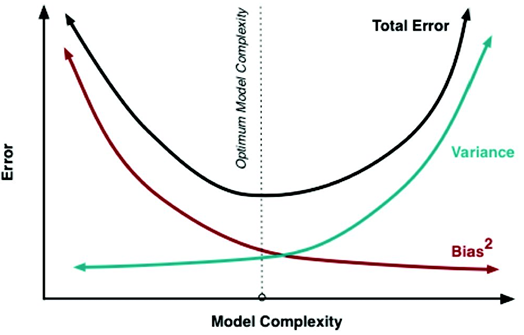
\includegraphics[width=1.0\linewidth]{figuresML/lesson_ml_3_pag_92.png}
    \end{minipage}
\end{figure}
\vspace{-7.5mm}
Since the generalization error (MSE) is the sum of bias squared and variance, achieving good generalization means finding the sweet spot that minimizes both. 

\subsection{Regularization for CNNs}
When dealing with inherently high-capacity models like deep neural networks, regularization acts as a control mechanism: it artificially restricts the model, reducing variance and closing the generalization gap without heavily increasing the bias. In practice, regularization techniques are all based on introducing a "noise" or a confounding factor to our network to prevent it from memorizing the training data. Adding a penalty does this by confounding the loss function, while batch normalization does this by normalizing the inputs on a batch during training.

We have already mentioned the dropout, penalty and batch normalization techniques for regularization. For Convolutional Neural Networks, another incredibly efficient way to regularize the model is \textbf{data augmentation}. By applying various transformations to our data (such as zooming, rotation, elastic deformation, blurring, or adding artificial noise) we artificially expand the training dataset. This forces the network to learn invariant, generalized features rather than memorizing the exact pixel layout of the original input. Here is an example of data augmentation for medical images. 

\begin{center}
    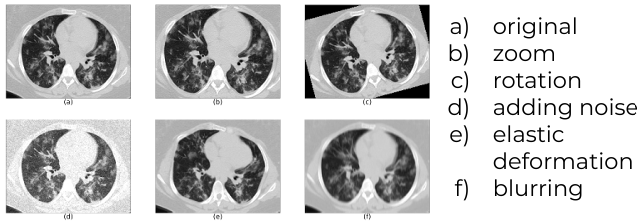
\includegraphics[width=0.5\linewidth]{figuresML/lesson_ml_3_pag_94.png}
\end{center}

Of course, data obtained in such a way will not be independent from the original, and the learning advantages will therefore be limited.

\subsection{Decision trees regularization and Ensembling}
While neural networks are extremely powerful, decision trees remain particularly suited for handling categorical variables and regression problems. However, a standard decision tree is highly prone to overfitting (high variance). To mitigate this, we can apply several regularization constraints:
\begin{itemize}
    \item[-] \textit{Minimum Leaf Size}: Sets the minimum number of samples required to form a terminal node. If too small (e.g., 1), the tree creates very specific, overfitted leaves. Larger values force the tree to be more general.
    \item[-] \textit{Maximum Depth}: Limits the number of levels in the tree. Deep trees capture noise, so setting a limit (e.g., \texttt{max\_depth = 5}) improves generalization.
    \item[-] \textit{Maximum Number of Nodes}: Restricts the total number of internal and leaf nodes, capping overall complexity.
    \item[-] \textit{Minimum Decrease in Loss}: A split is only executed if the improvement in the loss function (e.g., Gini, entropy, MSE) exceeds a certain threshold, preventing useless splits.
    \item[-] \textit{Pruning}: After building a full tree, branches that do not improve performance on a separate validation set are systematically removed.
\end{itemize}

To further combat the high variance inherent in decision trees, we rely on technique called \textbf{ensembling}. \\
Let's take $n$ random variables that are independently and identically distributed with variance $var(x)=\sigma^2$. The variance of their average is $var(\bar{x}) = \frac{\sigma^2}{n}$. If we drop the independence assumption, we introduce a correlation factor $\rho$:
\begin{equation}
    var(\bar{x}) = \rho\sigma^2 + \frac{1-\rho}{n}\sigma^2
\end{equation}
Ensembling is a technique that combines many models called \textit{weak learners} to obtain a more robust metamodel. Here $x_i$ does not represent a training sample, but a different model / decision tree. That's why it is useful to drop the independence assumption, since different models may be trained on the same dataset. By increasing the number of models $n$ and decreasing the correlation $\rho$ between them, the overall variance drops significantly. There are four main ways to do this: using different algorithms, using different training sets, implementing bagging or implementing boosting. Let's see how those work

\textbf{Bagging} or \textbf{Bootstrap Aggregating)} is a typical method used in statistics to measure uncertainty. To implement it we define bootstrap samples $Z \sim S$ (where $S$ is our original training sample), sampling $M$ times from the training set \textit{with replacement} (each subsample has the same dimension as the initial dataset but with duplicates and missing data). We train a single model $G_m$ on each bootstrap sample, and we define the metamodel by averaging their outputs:
\begin{equation*}
   G(m) = \frac{\sum_{m=1}^M G_m(x)}{M}
\end{equation*}
The larger $M$ is, the smaller the variance. \newline\newline
This technique is fundamental for the so called \textit{Random Forest} algorithms. Bagging is well suited for decision trees because they inherently have high variance. However, to reduce correlation among single decision trees, random forests perform bagging plus a random subsampling in the feature space. This decreases the correlation term $\rho$.

Unlike bagging, where models are trained independently, \textbf{boosting} trains models sequentially. The logic follows a recursive pattern:
\begin{enumerate}
    \item We make the first split.
    \item We identify the mistakes made by the current model.
    \item We increase the weight of those misclassified samples.
    \item Now the new weak learner may choose another decision boundary focusing on the hardest samples.
    \item We apply this recursively.
\end{enumerate}
This logic is the foundation of algorithms like AdaBoost (applying weights to the hardest samples) or Gradient Boosting/XGBoost (finding the minimum of the residual error).


\subsection{More on optimizers}
The core of the learning process is the optimization of the cost function $J(\theta)$. We already saw the stochastic gradient descent and mini-batch stochastic gradient descent methods for optimization, which update the parameters $\theta_i$ of the algorithm as follows:
\begin{equation}
    \theta_j:=\theta_j - \alpha \dfrac{\partial J(\theta_j)}{\partial\theta_j}
\end{equation}
where $\alpha$ is the learning rate and $J(\theta_j)$ is the cost function.
However, to improve convergence, several advanced optimizers modify this basic update rule. Let's take a look at some of them.

\textbf{SGD with Momentum}:
We modify the parameter update by inserting a new parameter called "velocity" $v_t$, which accumulates past gradients:
\begin{equation}
\begin{aligned}
    v_t &= \beta v_{t-1} + \frac{\partial J(\theta_j)}{\partial \theta_j} \\
    \theta_j &:= \theta_j - \alpha \left( \beta v_{t-1} + \frac{\partial J(\theta_j)}{\partial \theta_j} \right)
\end{aligned}
\end{equation}
The momentum coefficient $\beta$ (typically around 0.9) regulates how much past information is retained. This alleviates the problem of SGD stopping at local optima and reduces oscillations. However, if the local valleys are deep and momentum is exhausted, it can still get trapped in a local minimum.

\textbf{AdaGrad}:
AdaGrad provides an adaptive learning rate by tracking the sum of the squared gradients, $r_j^{(t)}$:
\begin{equation}
    r_j^{(t)} = r_j^{(t-1)} + \left(\frac{\partial J(\theta_j)}{\partial \theta_j}\right)^2 \quad \Longrightarrow \quad \theta_j := \theta_j - \frac{\alpha}{\sqrt{r_j^{(t)}} + \epsilon} \frac{\partial J(\theta_j)}{\partial \theta_j}
\end{equation}
If a parameter has been strongly updated in the past, it will be updated a little less in the future. This works well with sparse data distributions, but in later stages, the sum of square gradients in the denominator becomes very large, causing the parameter update to approach zero prematurely.

\textbf{RMSprop}:
RMSprop fixes AdaGrad's vanishing learning rate by replacing the accumulator with an exponential moving average:
\begin{equation}
    r_j^{(t)} = \beta r_j^{(t-1)} + (1-\beta)\left(\frac{\partial J(\theta_j)}{\partial \theta_j}\right)^2
\end{equation}
By progressively "forgetting" older gradients (regulated by the decay coefficient $\beta$), RMSprop avoids the continuous accumulation of the second momentum. It works incredibly well, though it can be unstable in the very early stages of optimization.

\textbf{Adam (Adaptive Moment Estimation)}:
Adam delightfully merges momentum and RMSprop by keeping track of both the first momentum and the second momentum, adding a correction for initialization bias:
\begin{align}
    m_t &= \beta_1 m_{t-1} + (1-\beta_1)\frac{\partial J(\theta_j)}{\partial \theta_j} \\
    v_t &= \beta_2 v_{t-1} + (1-\beta_2)\left(\frac{\partial J(\theta_j)}{\partial \theta_j}\right)^2
\end{align}
Bias corrections:
\begin{equation}
    \hat{m}_t = \frac{m_t}{1-\beta_1^t} \quad \text{and} \quad \hat{v}_t = \frac{v_t}{1-\beta_2^t}
\end{equation}
Final update:
\begin{equation}
    \theta_j := \theta_j - \alpha \frac{\hat{m}_t}{\sqrt{\hat{v}_t} + \epsilon}
\end{equation}
Typically, hyperparameters are set to $\beta_1 = 0.9$, $\beta_2 = 0.999$, and $\epsilon = 10^{-8}$.

\section{Hands-on examples for neural networks (2)}

%left down right up
%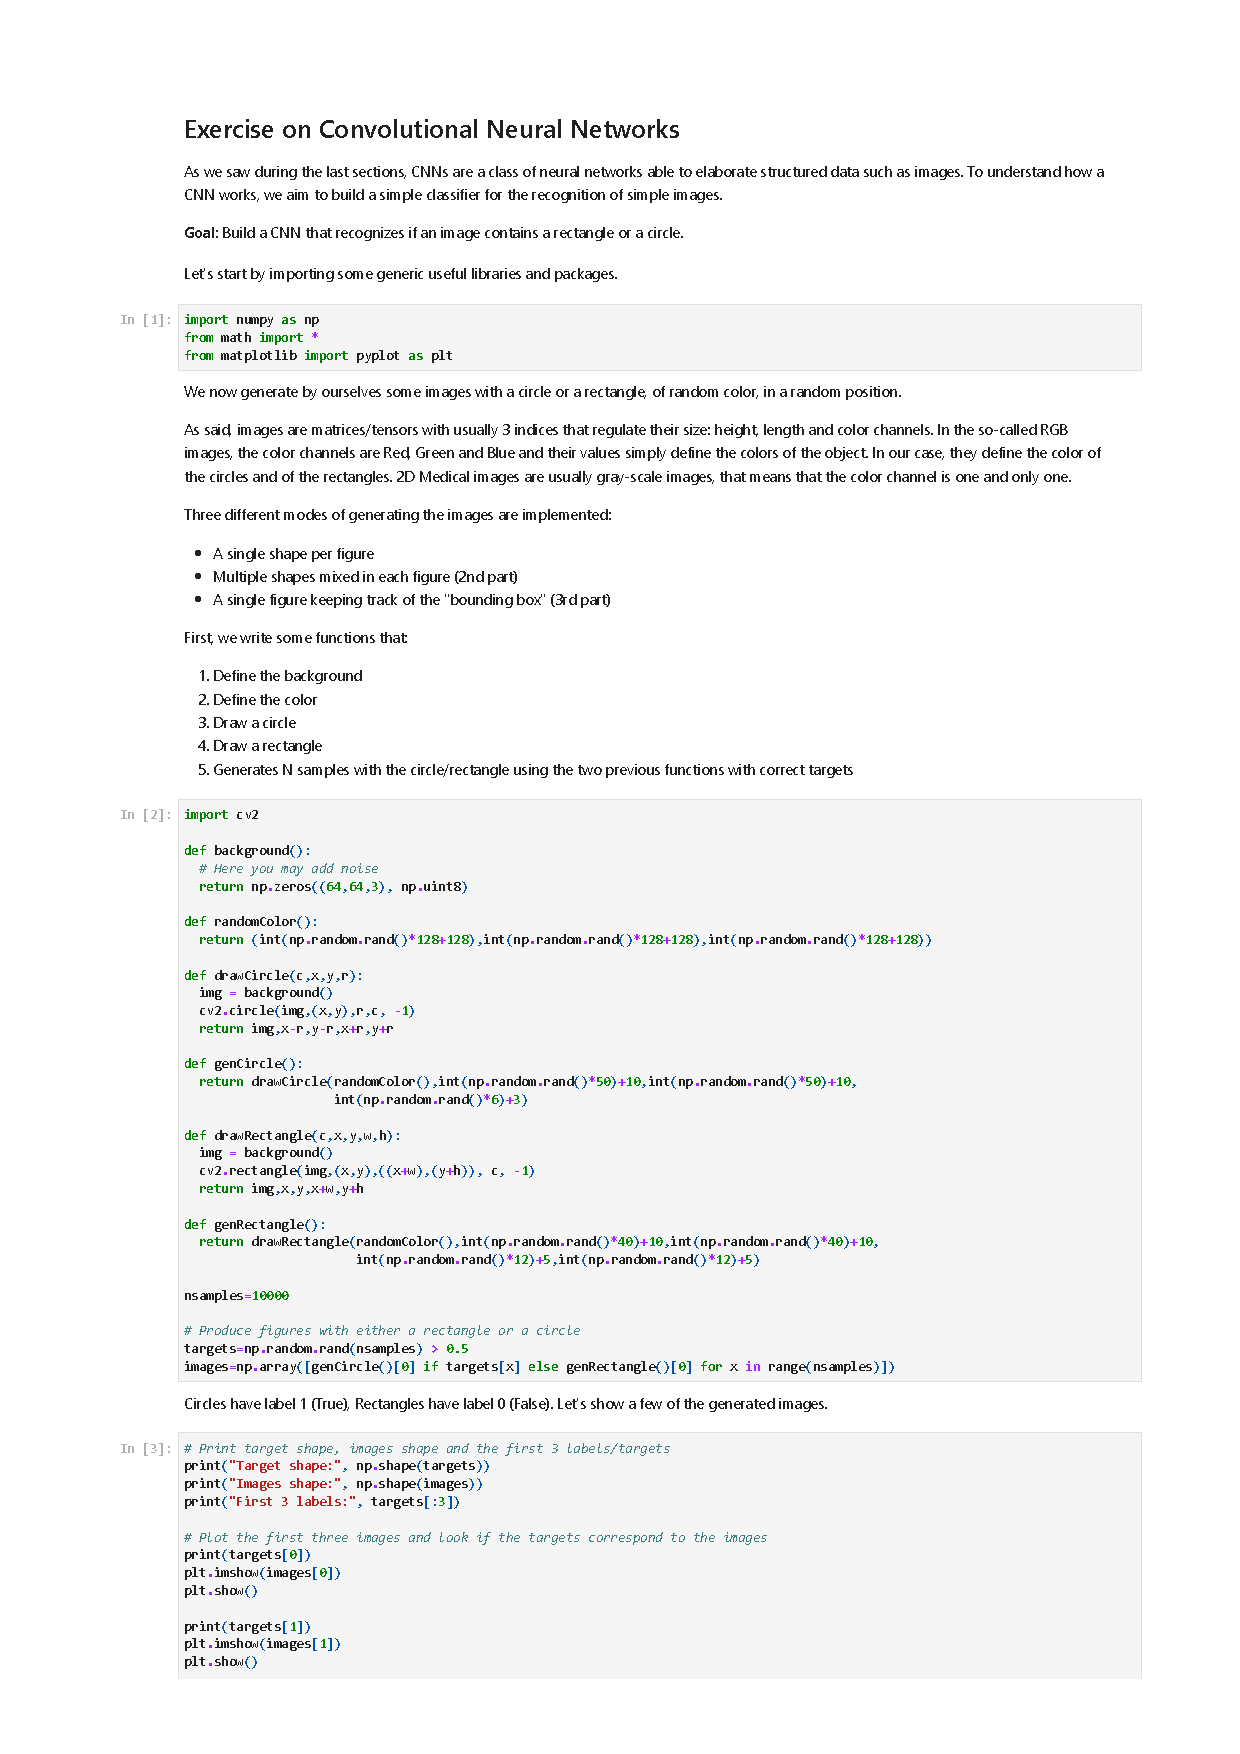
\includegraphics[page=1, width=0.85\textwidth, clip, trim=3cm 1cm 3cm 1.5cm]{lezioni/d_ML4_SOL.pdf}
%\includepdf[pages=2-]{lezioni/d_ML4_SOL.pdf}
% ML_3 nel mio Colab

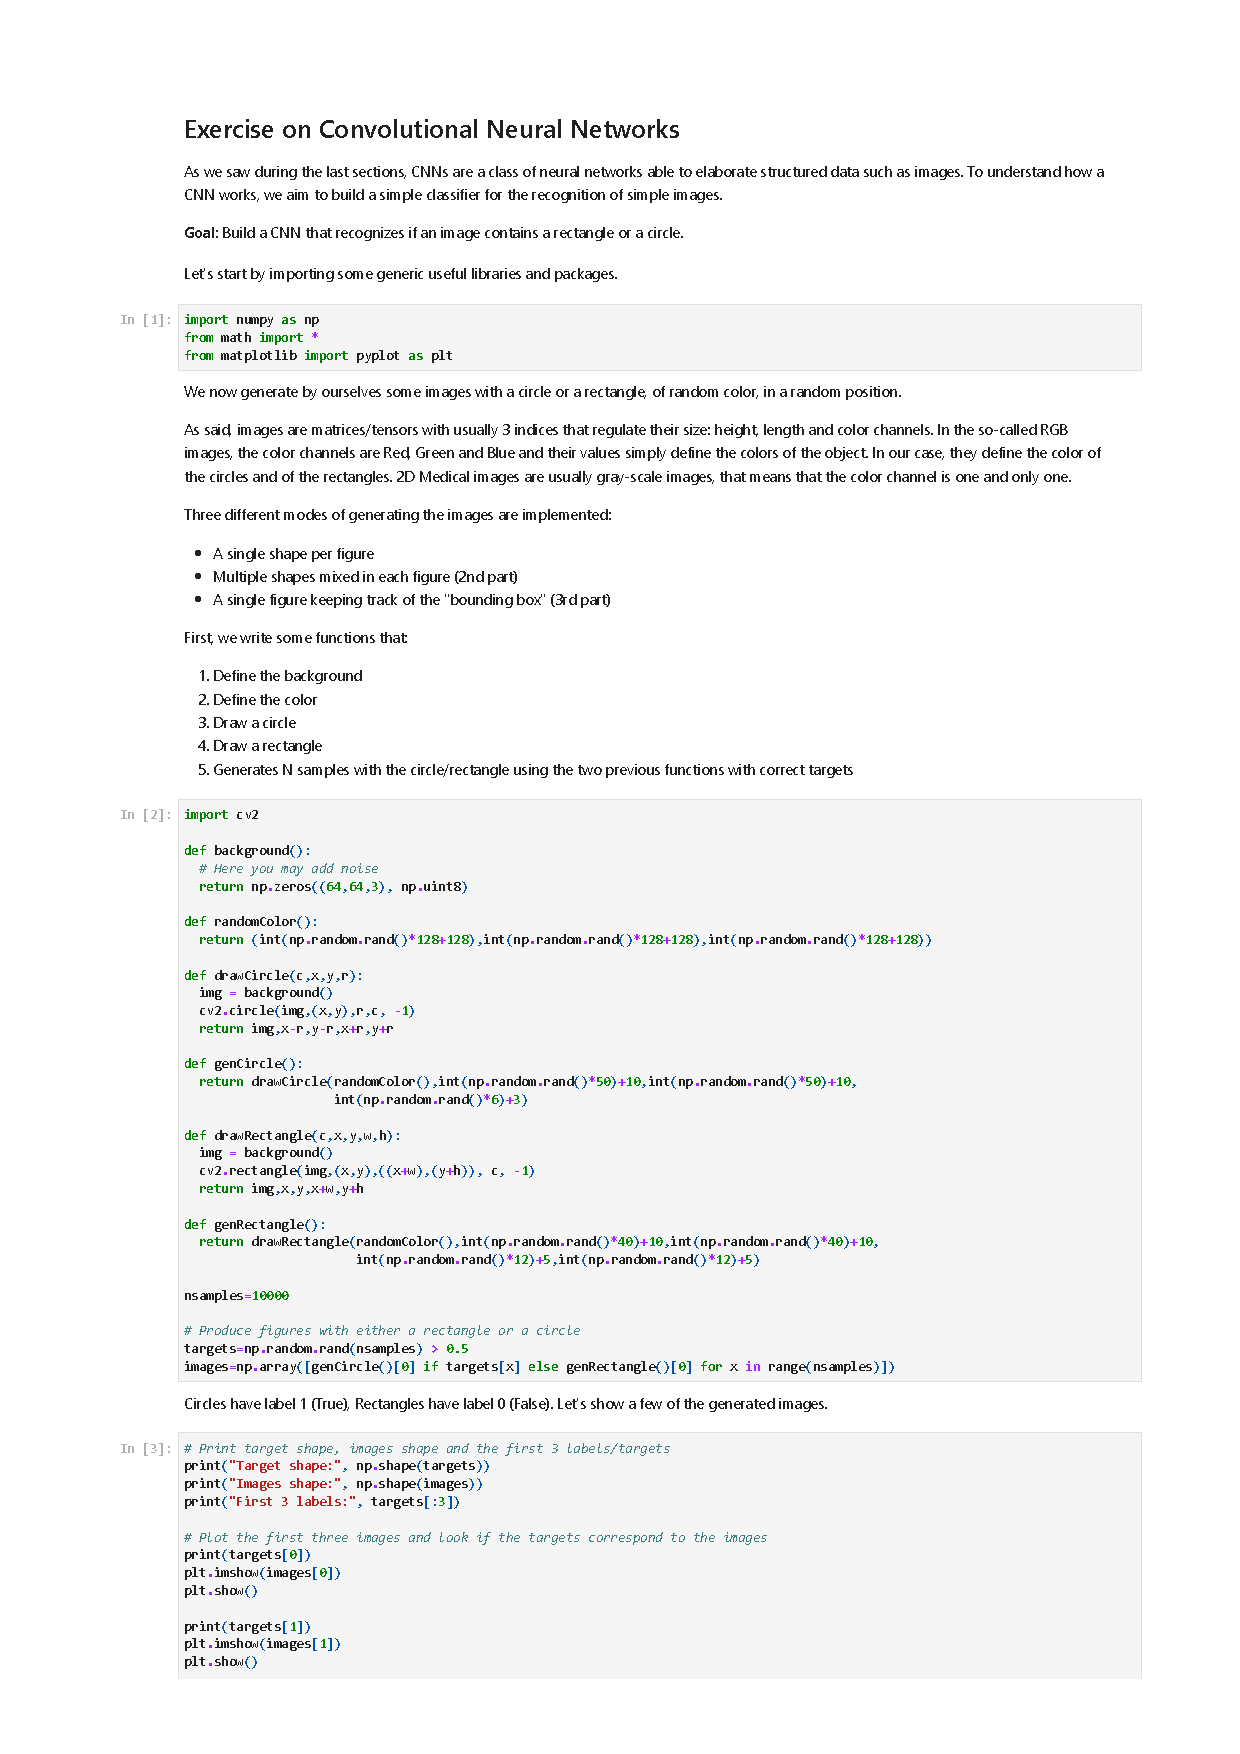
\includepdf[pages=-, pagecommand={\thispagestyle{plain}}]{lezioni/d_ML4_SOL.pdf} 
\section{An overview of generative models}

\subsection{What is a Generative Model?}
In traditional, deterministic machine learning models (such as those used for classification or regression), the network learns a fixed function $y = f(x)$ that maps an input to a specific, constant output. We train these deterministic models by minimizing a point-wise loss function, such as the mean squared error, which explicitly compares the predicted output point with the ground truth target point. \\
Generative models, on the other hand, are inherently \textit{stochastic}: if we run the inference of the neural network $N$ times, we expect to generate $N$ different outputs. Because of this stochasticity, we can no longer evaluate the network by strictly comparing individual points; instead, we must compare probability distributions. We want the network to learn a generated probability density function $q(x)$ that matches the true data probability density function $p(x)$.

To achieve this, we need a loss function capable of measuring the difference between two distributions. A common choice is the \textbf{Kullback-Leibler (KL) divergence}. The KL divergence from $q$ to $p$ is defined as:
\begin{equation}\label{eq:KL_div}
    D_{KL}(p||q) = \int p(x) \log \frac{p(x)}{q(x)} dx = \mathbb{E}_{x \sim p} [\log p(x) - \log q(x)]
\end{equation}
It is important to note that the KL divergence is not a true mathematical distance (even though it effectively acts like a "distance between the two distributions") because it is not symmetric ($D_{KL}(p||q) \neq D_{KL}(q||p)$) and it does not satisfy the triangle inequality. Nevertheless, it is more than adequate for machine learning purposes. \\
Notice that with this choice we can actually treat our loss function as a functional (much like the action in Lagrangian mechanics) and apply variational principles to minimize it, ensuring that our model's distribution $q(x)$ converges to the true distribution $p(x)$. Of course $q(x)$ has the weights $w$ of the model as parameters. Since we must restrict $q(x)$ to be a valid probability density function (i.e., its integral must equal 1 and non-negative), a Lagrange multiplier is typically added to the loss formulation to bound the minimization:
\begin{equation}
    L[q]=D_{KL}(p||q) + \lambda \int q(x) dx
\end{equation}
We can now search for the minimum of $L[q]$:
\begin{equation*}
\begin{aligned}
    \delta L[q]=\int [p(x)\log p(x) &- p(x)\dfrac{1}{q(x)}] \ \delta q \ dx \ + \ \lambda \int \delta q \ dx \quad \Rightarrow \\
    \frac{\delta L[q]}{\delta q(x)} &= -\frac{p(x)}{q(x)} + \lambda = 0 \quad \Rightarrow
\end{aligned}
\end{equation*}
\begin{equation}
    q(x) = \frac{p(x)}{\lambda}
\end{equation}
To find the specific value of $\lambda$, we enforce the normalization constraint $\int q(x) dx = 1$:
\begin{equation*}
    \int \frac{p(x)}{\lambda} dx = 1 \quad \Rightarrow \quad \frac{1}{\lambda} \int p(x) dx = 1
\end{equation*}
Since $p(x)$ is the true data distribution, it is already a valid probability density function, meaning $\int p(x) dx = 1$. Therefore:
\begin{equation}
    \lambda = 1
\end{equation}
Substituting $\lambda = 1$ back into our stationary solution, we arrive at the \textit{theoretical global minimum}:
\begin{equation}
    q(x) = p(x)
\end{equation}
This analytical result demonstrates that minimizing the KL divergence under the normalization constraint guarantees that our generated distribution $q(x)$ converges exactly to the true data distribution $p(x)$.

\subsection{Autoencoders and Variational Autoencoders (VAEs)}
Before discussing pure generative models, let us briefly revisit the concept of dimensionality reduction. A classic technique is the Principal Component Analysis (PCA) we mentioned in the first section of the module, which diagonalizes the covariance matrix to find the directions of maximum variance. However, PCA is strictly limited to linear transformations (essentially rotating the axes). If your data lies on a complex, non-linear manifold (e.g., a circle), PCA will fail to capture the true underlying structure because it cannot perform the necessary non-linear transformations, like converting to polar coordinates.

Autoencoders solve this by using neural networks to perform non-linear dimensionality reduction. An autoencoder (represented below with a vector input) consists of an \textit{encoder} network that maps the high-dimensional input $x$ into a much smaller, low-dimensional \textit{latent representation} $z$, and a \textit{decoder} network that reconstructs the original input from $z$ as output $\hat{x}$. The network is trained using an unsupervised approach by minimizing the reconstruction error between the input and the output, so the loss function will be something like $L \sim (x-\hat{x})^2$.

\begin{center}
    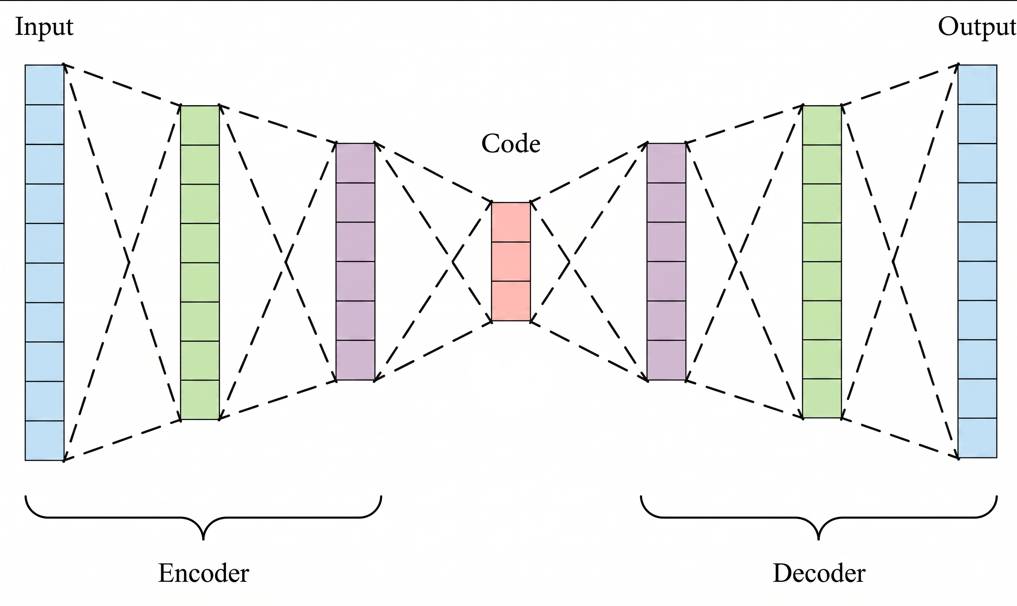
\includegraphics[width=0.6\textwidth]{figuresML/lesson_ml_5_pag_7.png}
\end{center}

The fundamental idea behind this architecture is to learn a meaningful representation of the data in the latent space $Z$ (e.g., defined by coordinates $z_1$ and $z_2$). For instance, if we train the autoencoder using images of dogs and cats as inputs, the network will learn to map these distinct classes to different, clustered regions within this latent space. The network effectively encodes the essential information required to reconstruct the output from the input, guided by the loss function.

Crucially, this process necessitates dimensionality reduction, often referred to as a bottleneck. Imagine if we were to design the architecture inversely: expanding the hidden layers so that the dimension of $Z$ is significantly larger than the input space $X$. This approach would fail because the neural network would simply learn the identity mapping, essentially approximating the function $f(x) = x$. The network could just pass the input image through without applying any meaningful filter, effectively turning off the redundant neurons. 

Therefore, the bottleneck forces the network to compress the data and extract the true underlying structure. As a natural consequence of this compression and subsequent reconstruction from the posterior, the quality of the reconstructed image $\hat{x}$ will inherently be slightly degraded compared to the original input.

However, a standard autoencoder is not a true generative model because the latent space $Z$ is not regularized. What does this mean? Knowing that the encoder maps the input $x$ into a single point in the latent space, if we sample a random point from the latter that lies between two encoded training examples (see figure), the decoder will likely produce nonsensical noise because it never learned what to do with that specific empty region of space. This makes extrapolation and interpolation in an unconstrained latent space highly unstable.

\begin{center}
    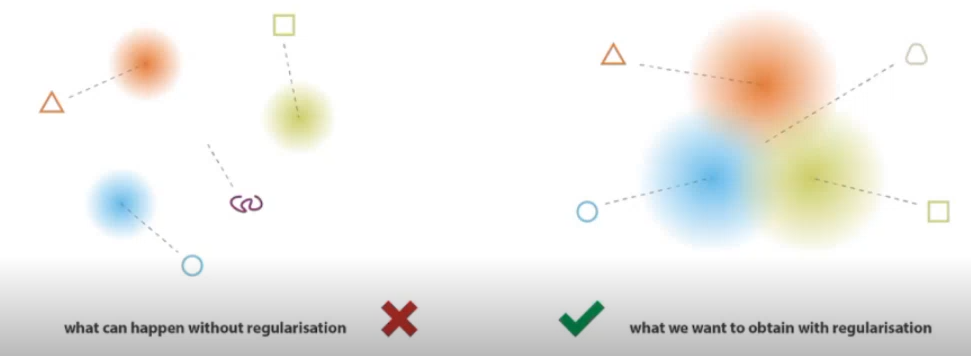
\includegraphics[width=0.7\textwidth]{figuresML/lesson_ml_5_pag_10.png}  
\end{center}

To make the autoencoder stochastic and fully generative, we use the \textbf{Variational Autoencoder (VAE)}. Instead of encoding an input $x$ into a single deterministic point $z$, the probabilistic encoder maps $x$ to the mean $\mu$ and standard deviation $\sigma$ of a Gaussian distribution, as shown in the following figure. We then sample the latent vector $z = \mu + \sigma \odot \epsilon$ (where $\epsilon \sim \mathcal{N}(0, I)$) and pass it to the decoder. By forcing the latent representations to follow a known distribution (like a Gaussian), we ensure the latent space is smooth and meaningful. This allows us to sample arbitrary points in the latent space and generate coherent, novel outputs, or gracefully interpolate between two different concepts. \\
To sum up, the key idea of VAEs is to introduce stochasticity during inference by regularizing the latent space ($\equiv$ "make it smooth"). We will take a look at the structure of a real-life VAE in the following hands-on section.

\begin{center}
    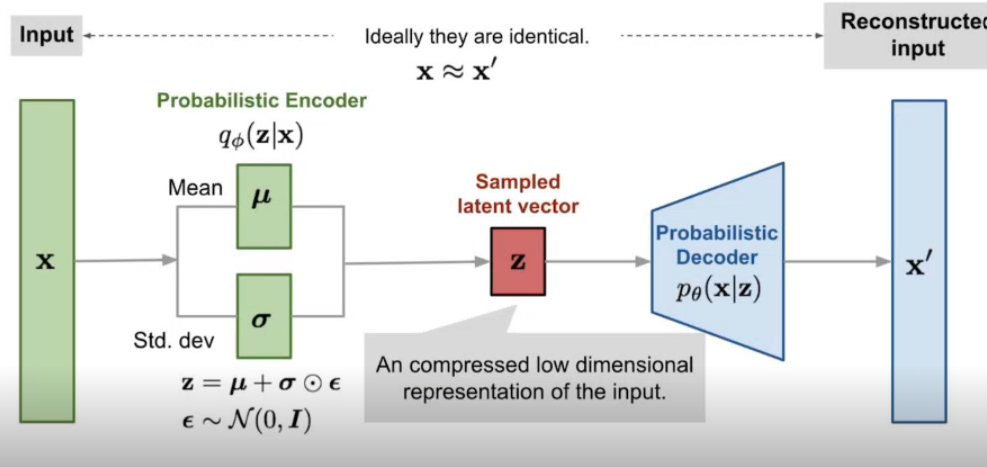
\includegraphics[width=0.8\textwidth]{figuresML/lesson_ml_5_pag_11.png}
\end{center}

Meaningful, smooth latent space representations are great for tasks like anomaly detection or data compression, and VAEs can interpolate between data points in a meaningful way in the latent space (e.g. you train your algorithm with images of cats and Van Gogh paintings, and you are able to generate an image of a cat painted in the style of Van Gogh). However, despite their elegance and flexibility, VAEs suffer from several known issues which are starting to make them obsolete:
\begin{itemize}
    \item[-] \textit{Mode collapse}: The model can generate a limited variety of outputs; 
    \item[-] \textit{Blurriness in outputs}: Due to dimensionality reduction, VAEs often produce blurrier results, especially in image generation tasks;
    \item[-] \textit{Complex training}: It is not easy to balance loss terms and regularize the phase space;
    \item[-] \textit{Limited expressiveness}: The assumption of a Gaussian prior limits the expressiveness of the model, impacting the variety of generated data.
\end{itemize}

\subsection{Generative Adversarial Networks (GANs)}\label{sec:intro_GAN}

\textbf{Generative Adversarial Networks (GANs)} represent a somewhat more "brute-force" approach to generation compared to the models discussed previously. The fundamental shift in this architecture is the origin of stochasticity: instead of injecting randomness into an intermediate latent space, it enters directly at the input stage, by feeding the network a random noise vector, which serves as the raw material for the generation process.

A GAN consists of two independent neural networks that work in tandem, effectively "competing" against each other:
\begin{itemize}
    \item[-] \textbf{Generator ($G$)}: This network takes the random noise vector $r$ and creates a synthetic data point, such as an image, effectively learning a function $G(r) = x_{\text{fake}}$. 
    %To force the generator to produce meaningful outputs rather than simply mapping noise to noise, it is pitted against an adversar.
    \item[-] \textbf{Discriminator ($D$)}: This network receives a mixture of real samples from the original training dataset and fake samples produced by the generator. Its objective is to correctly discriminate between them, assigning a label of real or fake.
\end{itemize}

\begin{center}
    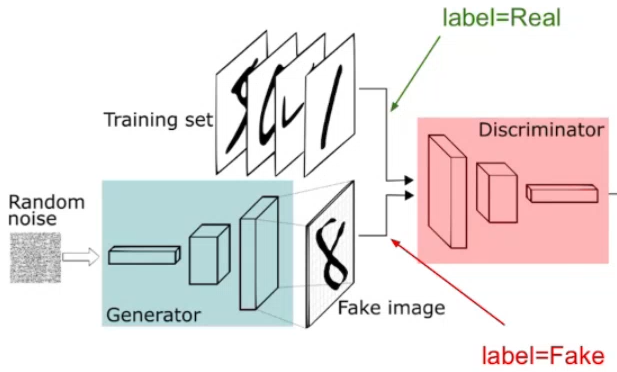
\includegraphics[width=0.6\textwidth]{figuresML/lesson_ml_5_pag_13.png}
\end{center}

At first glance, the discriminator's task appears to be a standard supervised learning problem because it relies on truth labels. However, the approach is fundamentally unsupervised because these labels are automatically defined by the system, so even if you inherently know which images were generated and which are from the true dataset, no manual annotation is needed.

The core dynamic of a GAN is defined as a \textbf{min-max problem}. The discriminator's goal is to distinguish the original training samples from the generated ones, maximizing its ability to catch fakes, while the generator attempts to fool the discriminator by creating increasingly realistic samples. Ultimately, this means minimizing a loss function with respect to the generator while maximizing a loss function with respect to the discriminator, driving both networks to continuously improve.

To understand how this tandem training works in practice, let's take a look at the mathematical formulation of the loss function. \\
The discriminator $D$ acts as a binary classifier whose output represents a probability that the given input is real, yielding a value between 0 and 1. Its goal is to maximize its accuracy, which translates to maximizing the following objective function:
\begin{equation}
    \max_D \mathcal{L}_D = \mathbb{E}_{x}[\log D(x)] + \mathbb{E}_{z}[\log(1 - D(G(z)))]
\end{equation}
We can break down the discriminator's logic into two distinct parts:
\begin{itemize}
    \item[-] For a real input $x$ from the training set, we want the discriminator to confidently predict 1. Therefore, we maximize the expected value of the logarithm of the discriminator's output, $\mathbb{E}_{x}[\log D(x)]$. 
    \item[-] For a fake image $G(z)$ generated from random noise $z$, we want the discriminator to confidently predict 0. This means minimizing the output $D(G(z))$, which is mathematically equivalent to maximizing the expected value of the complement, $\mathbb{E}_{z}[\log(1 - D(G(z)))]$. This conceptually aligns with penalizing the discriminator when it incorrectly labels a fake image as real.
\end{itemize}
Conversely, the generator $G$ is solely focused on fooling the discriminator. It wants the discriminator to output a value as close to 1 as possible for the fake images. Therefore, the generator's objective is to minimize the second term of the discriminator's loss:
\begin{equation}
    \min_G \mathcal{L}_G = \mathbb{E}_{z}[\log(1 - D(G(z)))]    
\end{equation}
When the generator is successfully minimizing this function, it implies that the discriminator is doing a poor job, meaning the generated images $G(z)$ look incredibly similar to the true input $x$. This is what we mean by a min-max problem: since the two networks are optimizing the same function in opposite directions, as training progresses the generator is forced to produce increasingly realistic structures to keep fooling an improving discriminator.

While GANs produce much sharper and more realistic images than VAEs since they are not subject to dimensionality reduction, their training dynamics are notoriously unstable. It is difficult to reach a good equilibrium between generator and discriminator, and GANs usually suffer from \textbf{mode collapse} (the generator might start producing the exact same realistic output repeatedly regardless of the input noise) and more importantly \textbf{vanishing gradient problems}. Intuitively, if the discriminator becomes too perfect too quickly, the generator receives no useful gradient information to improve its outputs.

To address the critical issue of vanishing gradients and training instability, instead of relying on a binary classification approach that minimizes a probabilistic divergence, an advanced formulation introduces concepts from the so-called \textit{Optimal Transport Theory}. In general, we seek the transformation $\mathcal{T}_{X \to Y}$ that requires the least number of steps ($\equiv$ the least amount of energy) to map a space $X$ to a space $Y$. In our case, this effort to minimize the transformation cost is formalized by the \textbf{Wasserstein Distance} (commonly known as the \textbf{Earth Mover's distance}), which provides a robust measure of the distance between the distribution of real data and the generated one. In this architecture, known as the \textbf{Wasserstein GAN (WGAN)}, the traditional discriminator is replaced by a \textbf{critic} network, denoted as $f_w(x)$ \footnote{A crucial mathematical requirement for this objective function to be valid is that the critic $f_w$ must be trained to learn a \textit{Lipschitz continuous} function. Although enforcing this Lipschitz constraint in practice is not trivial, the theoretical payoff is significant.}. Rather than outputting a probability bounded between 0 and 1, the critic outputs a raw scalar value that directly evaluates the similarity (or difference) between the distributions. The loss function is then entirely reconfigured to approximate this Wasserstein distance ($W$) between the real data distribution $p_r$ and the generated fake data distribution $p_g$:
\begin{equation}
    \mathcal{L}(p_r, p_g) = W(p_r, p_g) = \max_{w \in W} \left( \mathbb{E}_{x \sim p_r}[f_w(x)] - \mathbb{E}_{z \sim p_r(z)}[f_w(g_\theta(z))] \right)
\end{equation}
The Wasserstein distance provides a much smoother, linear gradient compared to regular GANs. This ensures that even when the fake and real distributions are entirely disjoint, the generator still receives a steady, meaningful gradient signal, effectively solving the vanishing gradient problem. Take a look at \url{https://arxiv.org/abs/1701.07875} and at the Advanced Machine Learning chapter for more details.

\subsection{Normalizing flows}
Another approach to work with probability density functions is the so-called \textbf{normalizing flows} technique. The idea is to apply a chain of simple, invertible transformations to map a simple base distribution (like a multi-dimensional Gaussian) into the complex target distribution of our data. The transformations must be bijective (invertible), so we can easily travel back and forth between the simple space $Z$ (controlled and defined by the user) and the complex data space $X$, allowing us to explicitly calculate the exact likelihood of the data. In other words, we are not actually learning the probability density function, but the function $f$ that will let us compute it point by point starting from a simpler one. Here is a simple representation:
\begin{center}
    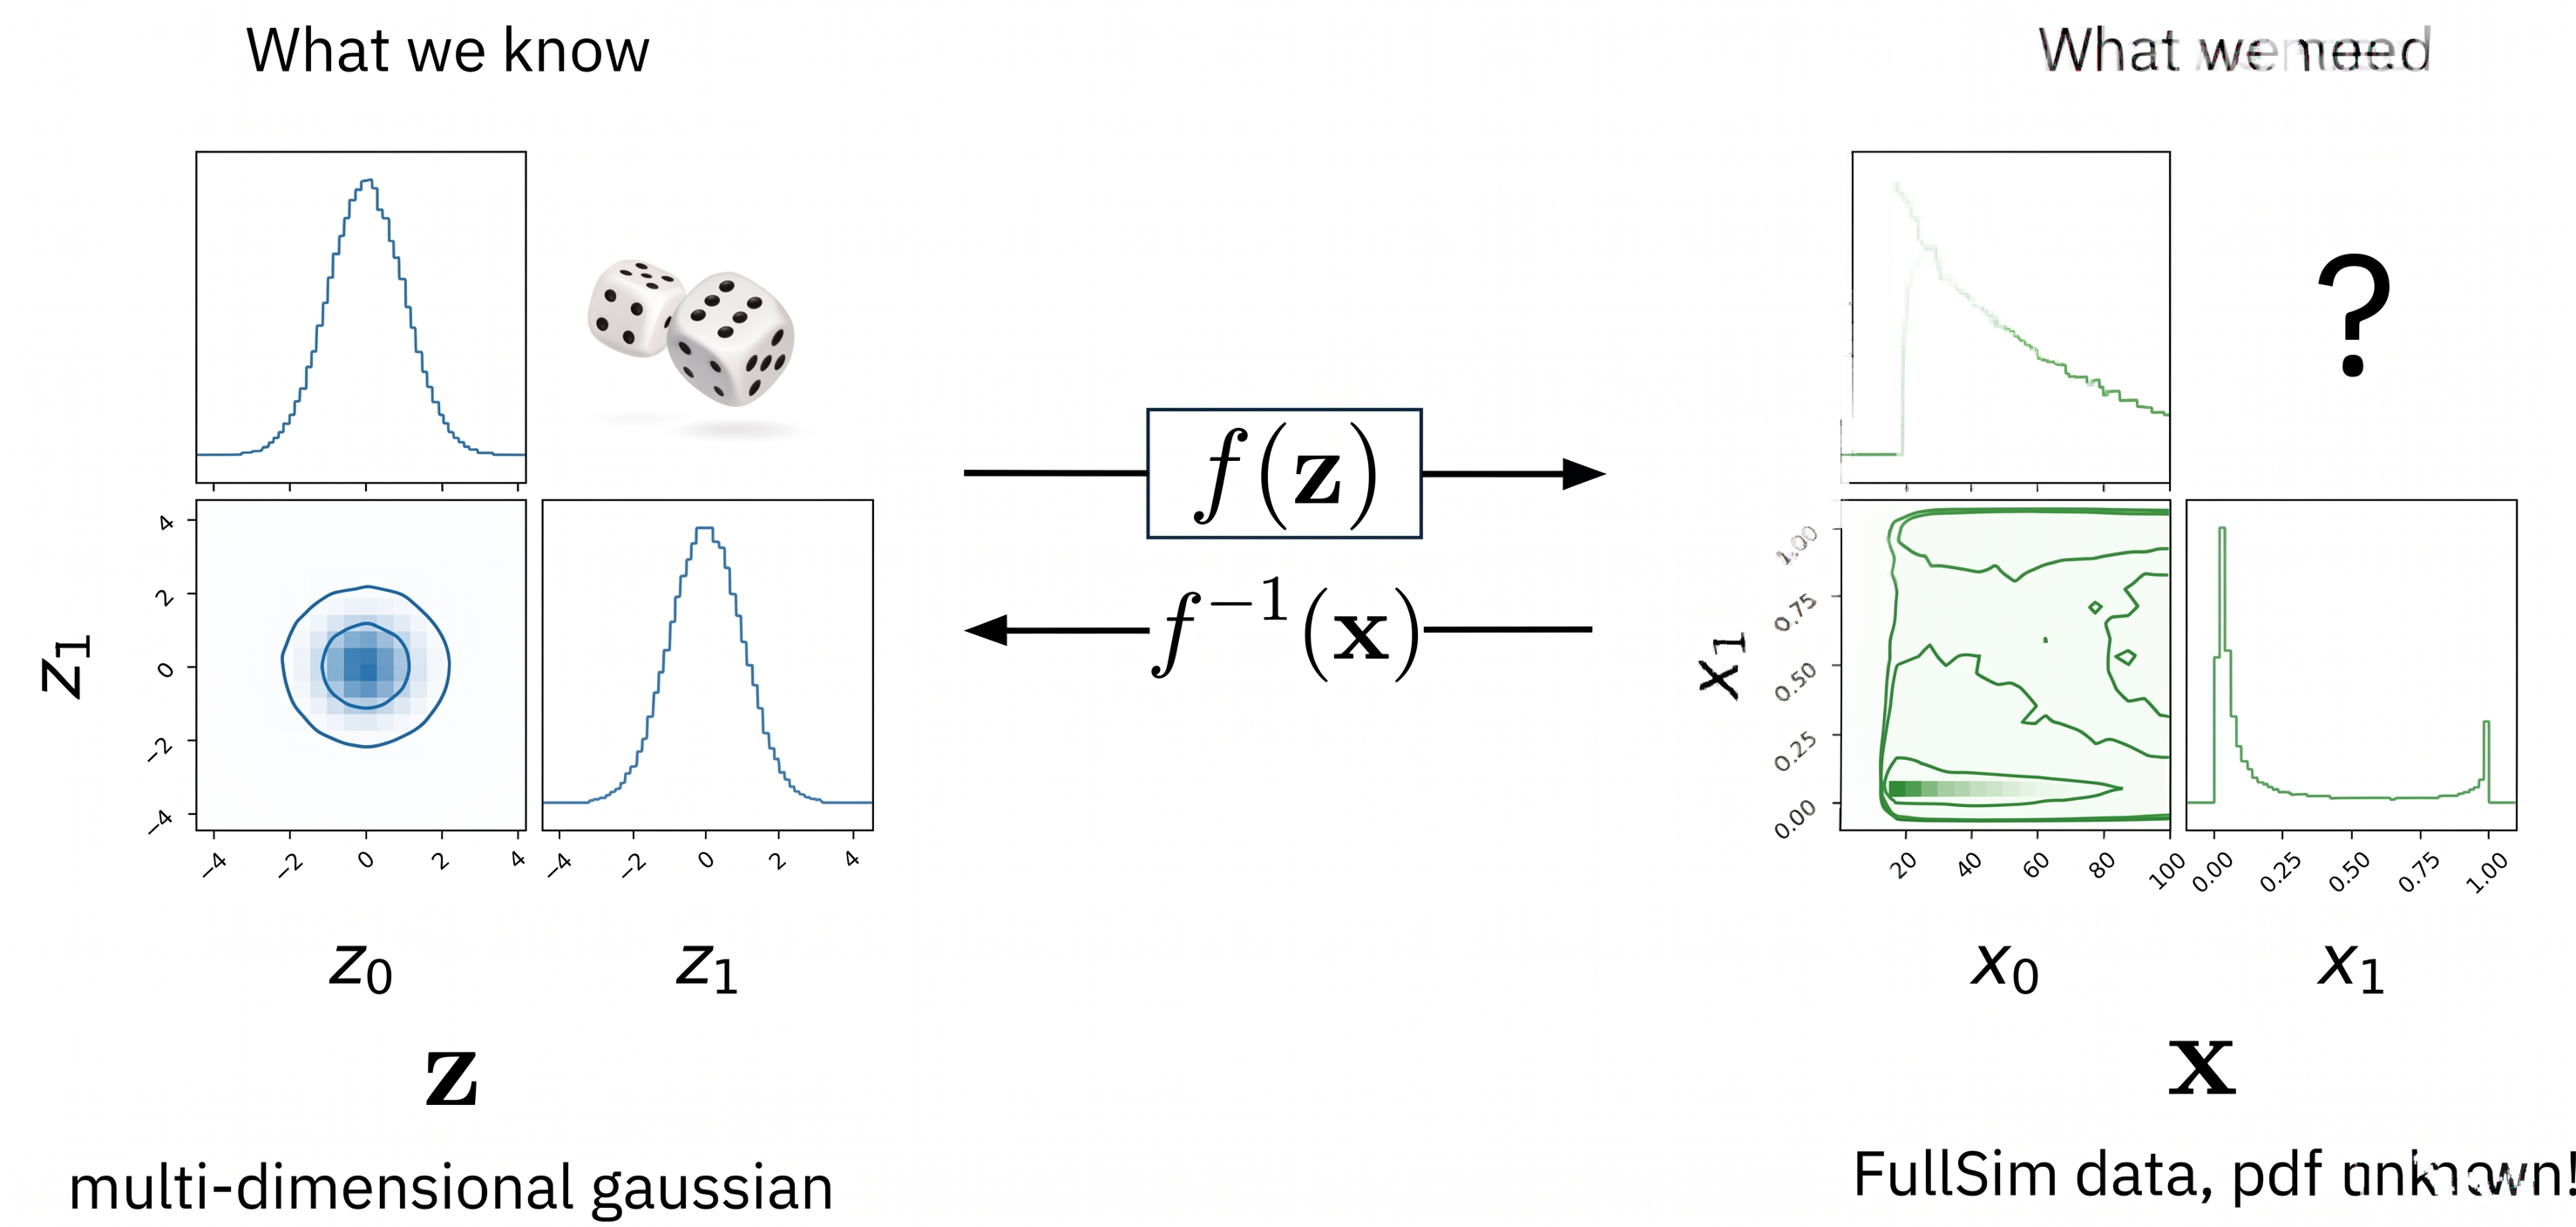
\includegraphics[width=0.8\textwidth]{figuresML/lesson_ml_5_pag_19.png}
\end{center}
There is an evident problem with this method: as you may imagine, inverting an arbitrary neural network is generally impossible. To maintain invertibility, normalizing flows rely on highly specific network architectures:
\begin{itemize}
    \item[-] \textbf{Autoregressive flows}: The network transforms variables sequentially. The first variable depends on nothing, the second depends only on the first, the third depends on the first and second, and so on (as shown below). This specific triangular structure makes calculating the Jacobian determinant and inverting the function computationally feasible.
    \begin{center}
        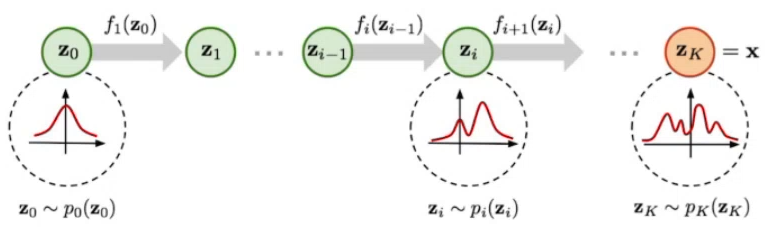
\includegraphics[width=0.8\textwidth]{figuresML/lesson_ml_5_pag_20.png}
    \end{center}
    \item[-] \textbf{Coupling layers}: The input vector is partitioned into two disjoint subsets, $x_A$ and $x_B$. The layer applies an identity mapping to one subset, while transforming the second subset using a function parameterized by a neural network conditioned on the first. Mathematically, the forward mapping to output $y = (y_A, y_B)$ is typically formulated as:
    \begin{equation*}
        \begin{cases}
            y_B = x_B \\
            y_A = x_A \cdot \exp(S(x_B))
        \end{cases}
    \end{equation*}
    where $S$ is an arbitrary neural network. The brilliance of this trick is its trivial invertibility: since $x_B$ is perfectly preserved as $y_B$, we can compute $S(y_B)$ and seamlessly apply the inverse operation (e.g., $x_A = y_A \cdot \exp(-S(y_B))$) to recover $x_A$ without ever needing to invert the neural network $S$ itself. To ensure the entire input space is fully transformed, consecutive coupling layers simply alternate which partition is passed through the identity mapping.
\end{itemize}

The modern evolution of this concept is known as \textbf{continuous flow}. Instead of relying on a sequence of discrete transformation layers to map a simple latent space to complex data, the process is modeled as a single, continuous transformation over time. 
The fundamental idea, trained via a technique called \textbf{flow matching}, is to start at time $t=0$ with a simple, easily sampleable distribution (like a Gaussian) and continuously morph it until $t=1$, where it matches the true target probability density function (p.d.f.):
\begin{equation*}
    \begin{cases}
        f(0; z) = z = \text{Gaussian} \\
        f(1; z) = \text{target p.d.f.}
    \end{cases}
\end{equation*}
To traverse this path, the variation of the distribution over an infinitesimal time step $dt$ is governed by a vector field, which effectively acts as the velocity required to move from the latent space $Z$ to the data space $X$. The DNN is explicitly tasked with learning this velocity field. Therefore, the continuous transformation can be described by the following differential equation:
\begin{equation*}
    f(t + dt) = f(t) + \text{DNN}(f(t)) \cdot dt
\end{equation*}
By integrating this learned velocity field over time, the model smoothly and efficiently transforms the random noise into the complex target distribution.

Another highly popular modern approach is \textbf{diffusion models}, which gradually add Gaussian noise to an image until it is completely destroyed, and then train a network to reverse the process, denoising the image step by step to generate new samples.

This was just a brief introduction to such methods, and we will dive a lot deeper into all the different flows and architectures summed up in the figure below during the Advanced Machine Learning chapter.

\begin{center}
    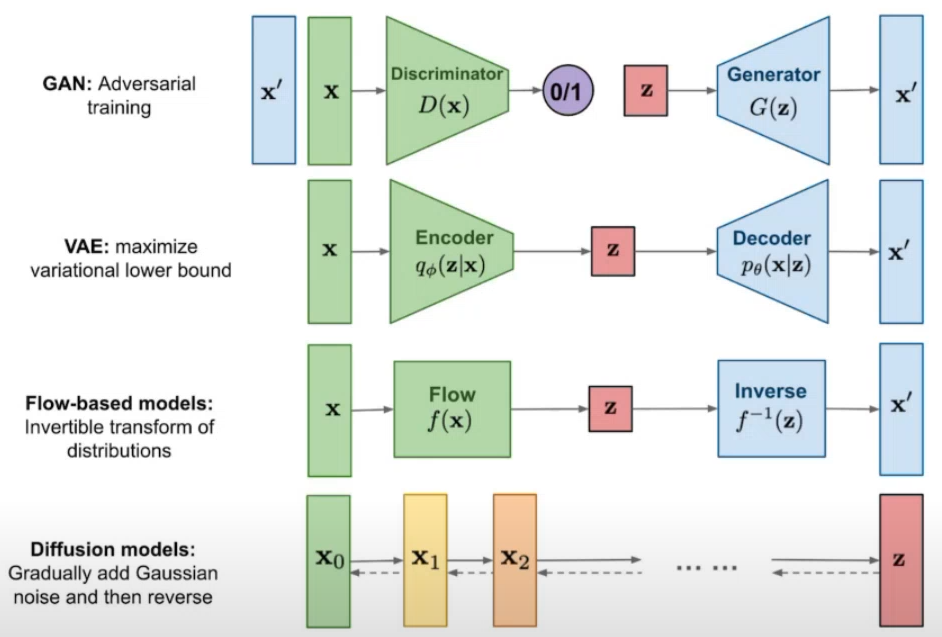
\includegraphics[width=0.65\textwidth]{figuresML/lesson_ml_5_pag_22.png}
\end{center}

\section{Hands-on example for Variational Autoencoders}

It is time to show how a Variational Autoencoder works in practice. Try to run the following Notebook by yourself, adjust the parameters and adapt it to different shapes.

You can find it here: \url{https://colab.research.google.com/drive/1TmONF8GWFJWSIn-3rDZEI_zV_NGccbbI?usp=sharing}.

%\includepdf[pages=-, pagecommand={\thispagestyle{plain}}]{lezioni/d_ML5_SOL.pdf} 

%ML_4 nel mio colab
\section{Hands-on example for Variational Autoencoders}
%\includepdf[pages=-, pagecommand={\thispagestyle{plain}}]{lezioni/d_ML5_SOL.pdf} 

%ML_4 nel mio colab
\section{Graph Neural Networks (GNNs)}\label{sec:GNN_intro}

\subsection{The need for graph-based architectures}
Graph Neural Networks were theorized long before the machine learning revolution that saw them take center stage. The beginning of their rapid rise in both the international market and academic research can be traced back to the 2018 paper available at this here: \url{https://arxiv.org/abs/1806.01261}.

In the landscape of modern machine learning, different architectures are highly optimized to exploit the specific symmetries of their input data. For instance, CNNs are the standard for computer vision because they process data structured on a multi-index euclidean grid (like the pixels of an image). By sliding a shared kernel across the grid, CNNs naturally exploit \textit{spatial translation equivariance}. Similarly, Recurrent Neural Networks (RNNs) or LSTMs (which we will see later) operate on sequentially ordered data (like text files), exploiting \textit{time-shift equivariance}. Generally speaking, a function $F$ is said to be equivariant (or often, though less appropriately, invariant) under a transformation $T$ if $F(T(t)) = T(F(t))$. The CNN example is straightforward: if we have an algorithm that identifies a cat in an image by overlaying a mask on it, shifting the cat by one pixel will result in the mask shifting by the exact same amount. Try to independently apply this same reasoning to RNNs and temporal equivariance.

However, in many scientific and industrial applications, data does not easily fit into a rigid tensor structure or a strict sequential order (where the position of an element carries a fixed physical meaning), representing what is known as \textbf{sparse data}. Consider datasets such as social networks, economic interactions, molecular structures, the galactic web in astrophysics, or functional MRI brain activity maps. In HEP, a particle collision at the LHC produces a "spray" of particles known as a jet, while the measurements from tracking and calorimeter detectors naturally form a scattered point cloud, not an ordered grid. 

\begin{center}
    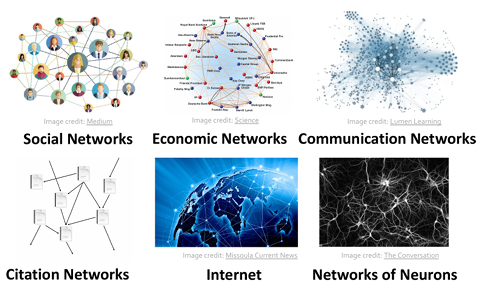
\includegraphics[width=0.32\textwidth]{figuresML/lesson_ml_5_pag_29a.png}
    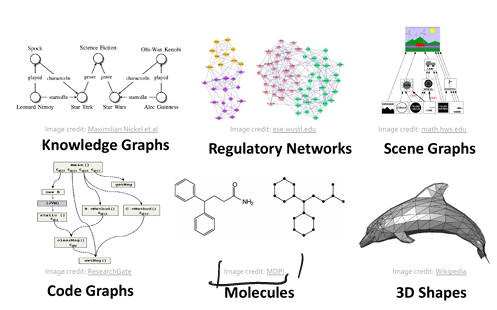
\includegraphics[width=0.32\textwidth]{figuresML/lesson_ml_5_pag_29b.png}
    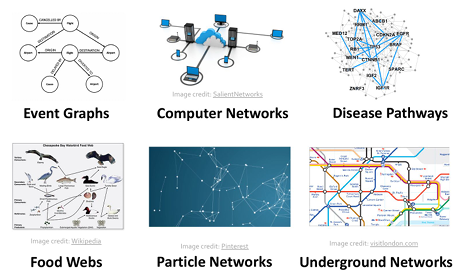
\includegraphics[width=0.32\textwidth]{figuresML/lesson_ml_5_pag_29c.png}
\end{center}

Attempting to cast this heterogeneous data into standard grid formats requires severe approximations, such as arbitrary binning (which leads to information loss) or the creation of highly sparse data structures filled primarily with zeros. To process this data natively, we require a structure that focuses on the nodes and their local connections, exploiting a new fundamental symmetry: \textbf{permutation equivariance} (or invariance). Because a point cloud has no inherent physical ordering, shuffling the input order of the points must yield the exact same overall result. This is the domain of \textbf{Graph Neural Networks (GNNs)}. \\ 
Generally speaking, an ML algorithm is easier to train the more the inherent equivariances of the problem are taken into account when designing its architecture. CNNs, LSTMs/GRUs, and GNNs are built to exploit equivariance under spatial translations, temporal translations, and permutations, respectively, thereby reducing both the number of parameters required for them to function and the necessary size of the training datasets. Extracting information from the local to the global scale (over tensor patches for CNNs and over small groups of connected nodes for GNNs) further increases their efficiency.\\
Recently GNNs were popularized by Google's DeepMind for weather forecast, which obtained similar or better results than state of the art non-ML models, but with less run time.

\subsection{From Deep-Sets to Graphs}
Imagine we now want to write the simplest possible algorithm that is equivariant to permutations, suitable for these point clouds. CNNs and RNNs must obviously be ruled out right away. 

To make things easier, let's consider a 3-body system where each point-like body is characterized by its position, velocity, and mass $(x, y, z, v_x, v_y, v_z, m)$. We want to write a NN that takes this system as input and outputs its energy. The algorithm we aim to develop is a so-called \textbf{Deep-Set} (DS)\footnote{The term Deep-Set refers to the fact that these algorithms are deep neural networks used to operate on sets (in the mathematical sense of the word) of inherently unordered data.}, and we will explain how it works by following this example.

The first step is, of course, to associate each body with a \textit{vertex} in the network. As we shall soon see, a vertex or node is the basic point-like structure of the graph, and for now you can imagine it as a connection point in a web-like structure. This is followed by a fundamental operation called \textit{embedding}, which we will encounter again in more complex GNNs and Transformers. It simply consists of a function $\phi_{emb}$ that takes the nodes as input and maps them into a much higher-dimensional space than the original one. In practice, $\phi_{emb}$ is a NN. 

In our example, we could have:
\begin{equation*}
    \phi_{emb}: \mathbb{R}^7 \longrightarrow \mathbb{R}^{100}, \quad \phi_{emb}(x_i) = h_i
\end{equation*}
Here, $h_i$ is called the \textit{hidden representation} of the node $x_i$.

Once all the nodes have been mapped, we can define an operation that preserves permutation equivariance and allows us to aggregate the data contained in all the $h_i$ vectors. We could choose, for instance, an element-wise sum, a maximum, or an average. In our example, let's consider:
\begin{equation*}
    h_{tot} = \rho(h_i) = \sum_i h_i \quad \text{with } \rho: \mathbb{R}^{100} \rightarrow \mathbb{R}^{100}, \ h_i \mapsto \sum_i h_i = h_{tot}
\end{equation*}

Once this is done, we can use a second neural network, $\mathcal{F}$, which takes $h_{tot}$ as input and returns the desired output. For the 3-body system, this corresponds to the total energy:
\begin{equation*}
    \mathcal{F}: \mathbb{R}^{100} \rightarrow \mathbb{R}, \quad h_{tot} \mapsto E_{tot}
\end{equation*}

To train this algorithm, i.e., to update the parameters of $\phi_{emb}$ and $F$, we can use the MSE as our loss function:
\begin{equation*}
    \mathcal{L} \propto \text{MSE}(E_{tot}, E_i)
\end{equation*}

This concludes the structure of a Deep-Set. In algorithms of this type, permutation invariance is guaranteed by the fact that $\phi_{emb}$ and $F$ are shared across all the vertices of the graph; i.e., the weights are shared by all nodes, similarly to what happens with sliding kernels in CNNs.

Notice that the use of Deep-Sets is limited by the fact that their output can only provide information about a global property of the system, rather than local ones. We cannot use this type of algorithm to predict, for example, where an individual body will be at a given time, even though it works reasonably well for calculating the total energy. This highlights the major advantage of modern GNNs, which instead allow for an "indexed" output that is specific to each individual node by exploiting the relationships between them.

\subsection{Anatomy of a Graph and Permutation equivariance}
A \textbf{graph} $G(V, E, u)$ is a highly flexible mathematical structure defined by three main components represented in figure:
\begin{center}
    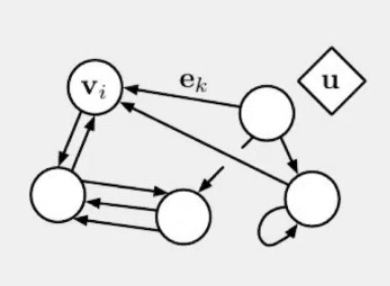
\includegraphics[width=0.32\textwidth]{figuresML/lesson_ml_5_pag_35.png}
\end{center}
\begin{itemize}
    \item[-] \textbf{Vertices/Nodes ($V$):} the fundamental entities of the graph. In a physical system, these could be planets, stars, or particles. Each node $v_i$ possesses \textbf{attributes} or \textit{features}, which hold the intrinsic information of the individual entities within the graph (e.g., mass, position, and velocity of the $i$-th body in the 3-body example).
    \item[-] \textbf{Edges ($E$):} the connections between vertices. Edges can be \textbf{directed} (one way) or \textbf{undirected} (bidirectional), and the number of edges connected to a specific vertex is called its \textbf{degree}. Edges $e_k$ represent relations or interactions, such as gravitational forces between bodies in our example or decay lineages between particles in other physical applications. \\
    Attributes can also be defined on the edges and once again, we can observe the enormous versatility of GNNs starting from our example: theoretically, given the positions of the bodies, we already possess all the information needed to deduce their mutual distances. We can therefore provide these as initial attributes on the edges, saving the GNN from spending resources and parameters to learn how to calculate them autonomously. Thus, we can decide to let the network learn to predict only the more complex relationships (e.g., the interaction forces between the bodies) to update the states of both nodes and edges, significantly improving its efficiency.
    \item[-] \textbf{Global state ($u$):} attributes that belong to the graph as a whole, rather than to any specific node or edge. Examples include the total energy or the overall angular momentum of a multi-body system. As outlined in the following figure, we can store the general properties of the graph in these global attributes.
\end{itemize}

\begin{center}
    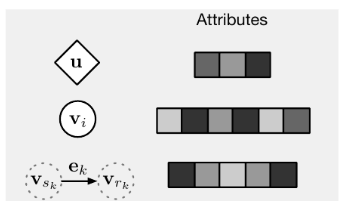
\includegraphics[width=0.4\linewidth]{figuresML/lesson_ml_5a_pag_8.png}
\end{center}

Just as CNNs apply the exact same convolutional kernel across different patches of an image, a GNN applies the exact same updating function to all nodes, one at a time. Because the function weights are shared, swapping node 1 with node 2 does not change the network's overall understanding of the system, perfectly preserving permutation equivariance. You will find much more detail at the following link: \url{https://arxiv.org/abs/1806.01261}.

\begin{figure}[H]
    \begin{minipage}[c]{0.75\textwidth}
        Graphs can be useful when your data is a list of values that would result in a sparse format if you try to bin it and put it on a grid (think for example about a jet of particles from LHC). Even if no actual link exists in sparse datasets, you can still use any type of clustering algorithm. For example, as long as some “distance” can be defined, a graph structure can be created looking at the $k$ nearest neighbors, where $k$ is a chosen integer, as represented in figure. Alternatively, if computational resources permit, we can initialize a fully connected graph where every node is linked to every other node.
    \end{minipage}\hfill
    \begin{minipage}[c]{0.25\textwidth}
        \centering
        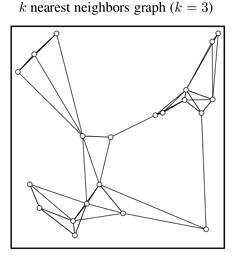
\includegraphics[width=0.9\linewidth]{figuresML/lesson_ml_5_pag_32.png}
    \end{minipage}
\end{figure}
\vspace{-7.5mm}

\subsection{Tasks on a Graph}
Depending on the specific goal of the analysis, GNNs are extremely versatile and can be applied to extract predictions at different levels of the graph hierarchy, as represented below:
\begin{itemize}
    \item[-] \textbf{Node-level tasks:} Predicting a label, type, or attribute for an individual node. An example in industry is detecting fake accounts within a massive social network; in physics, identifying the specific particle type of a given detector hit.
    \item[-] \textbf{Edge-level tasks:} Given a set of nodes, inferring missing edges or predicting the strength of a connection. For instance, predicting the probability that a user will buy a product, or in HEP, evaluating whether two separate particle tracks originated from the same primary vertex.
    \item[-] \textbf{Graph-level tasks:} Carrying out classification or regression over the entire graph. A classic example is predicting a molecule's overall toxicity based on its structural graph, or determining the total energy of a physical system.
\end{itemize}
\begin{center}
    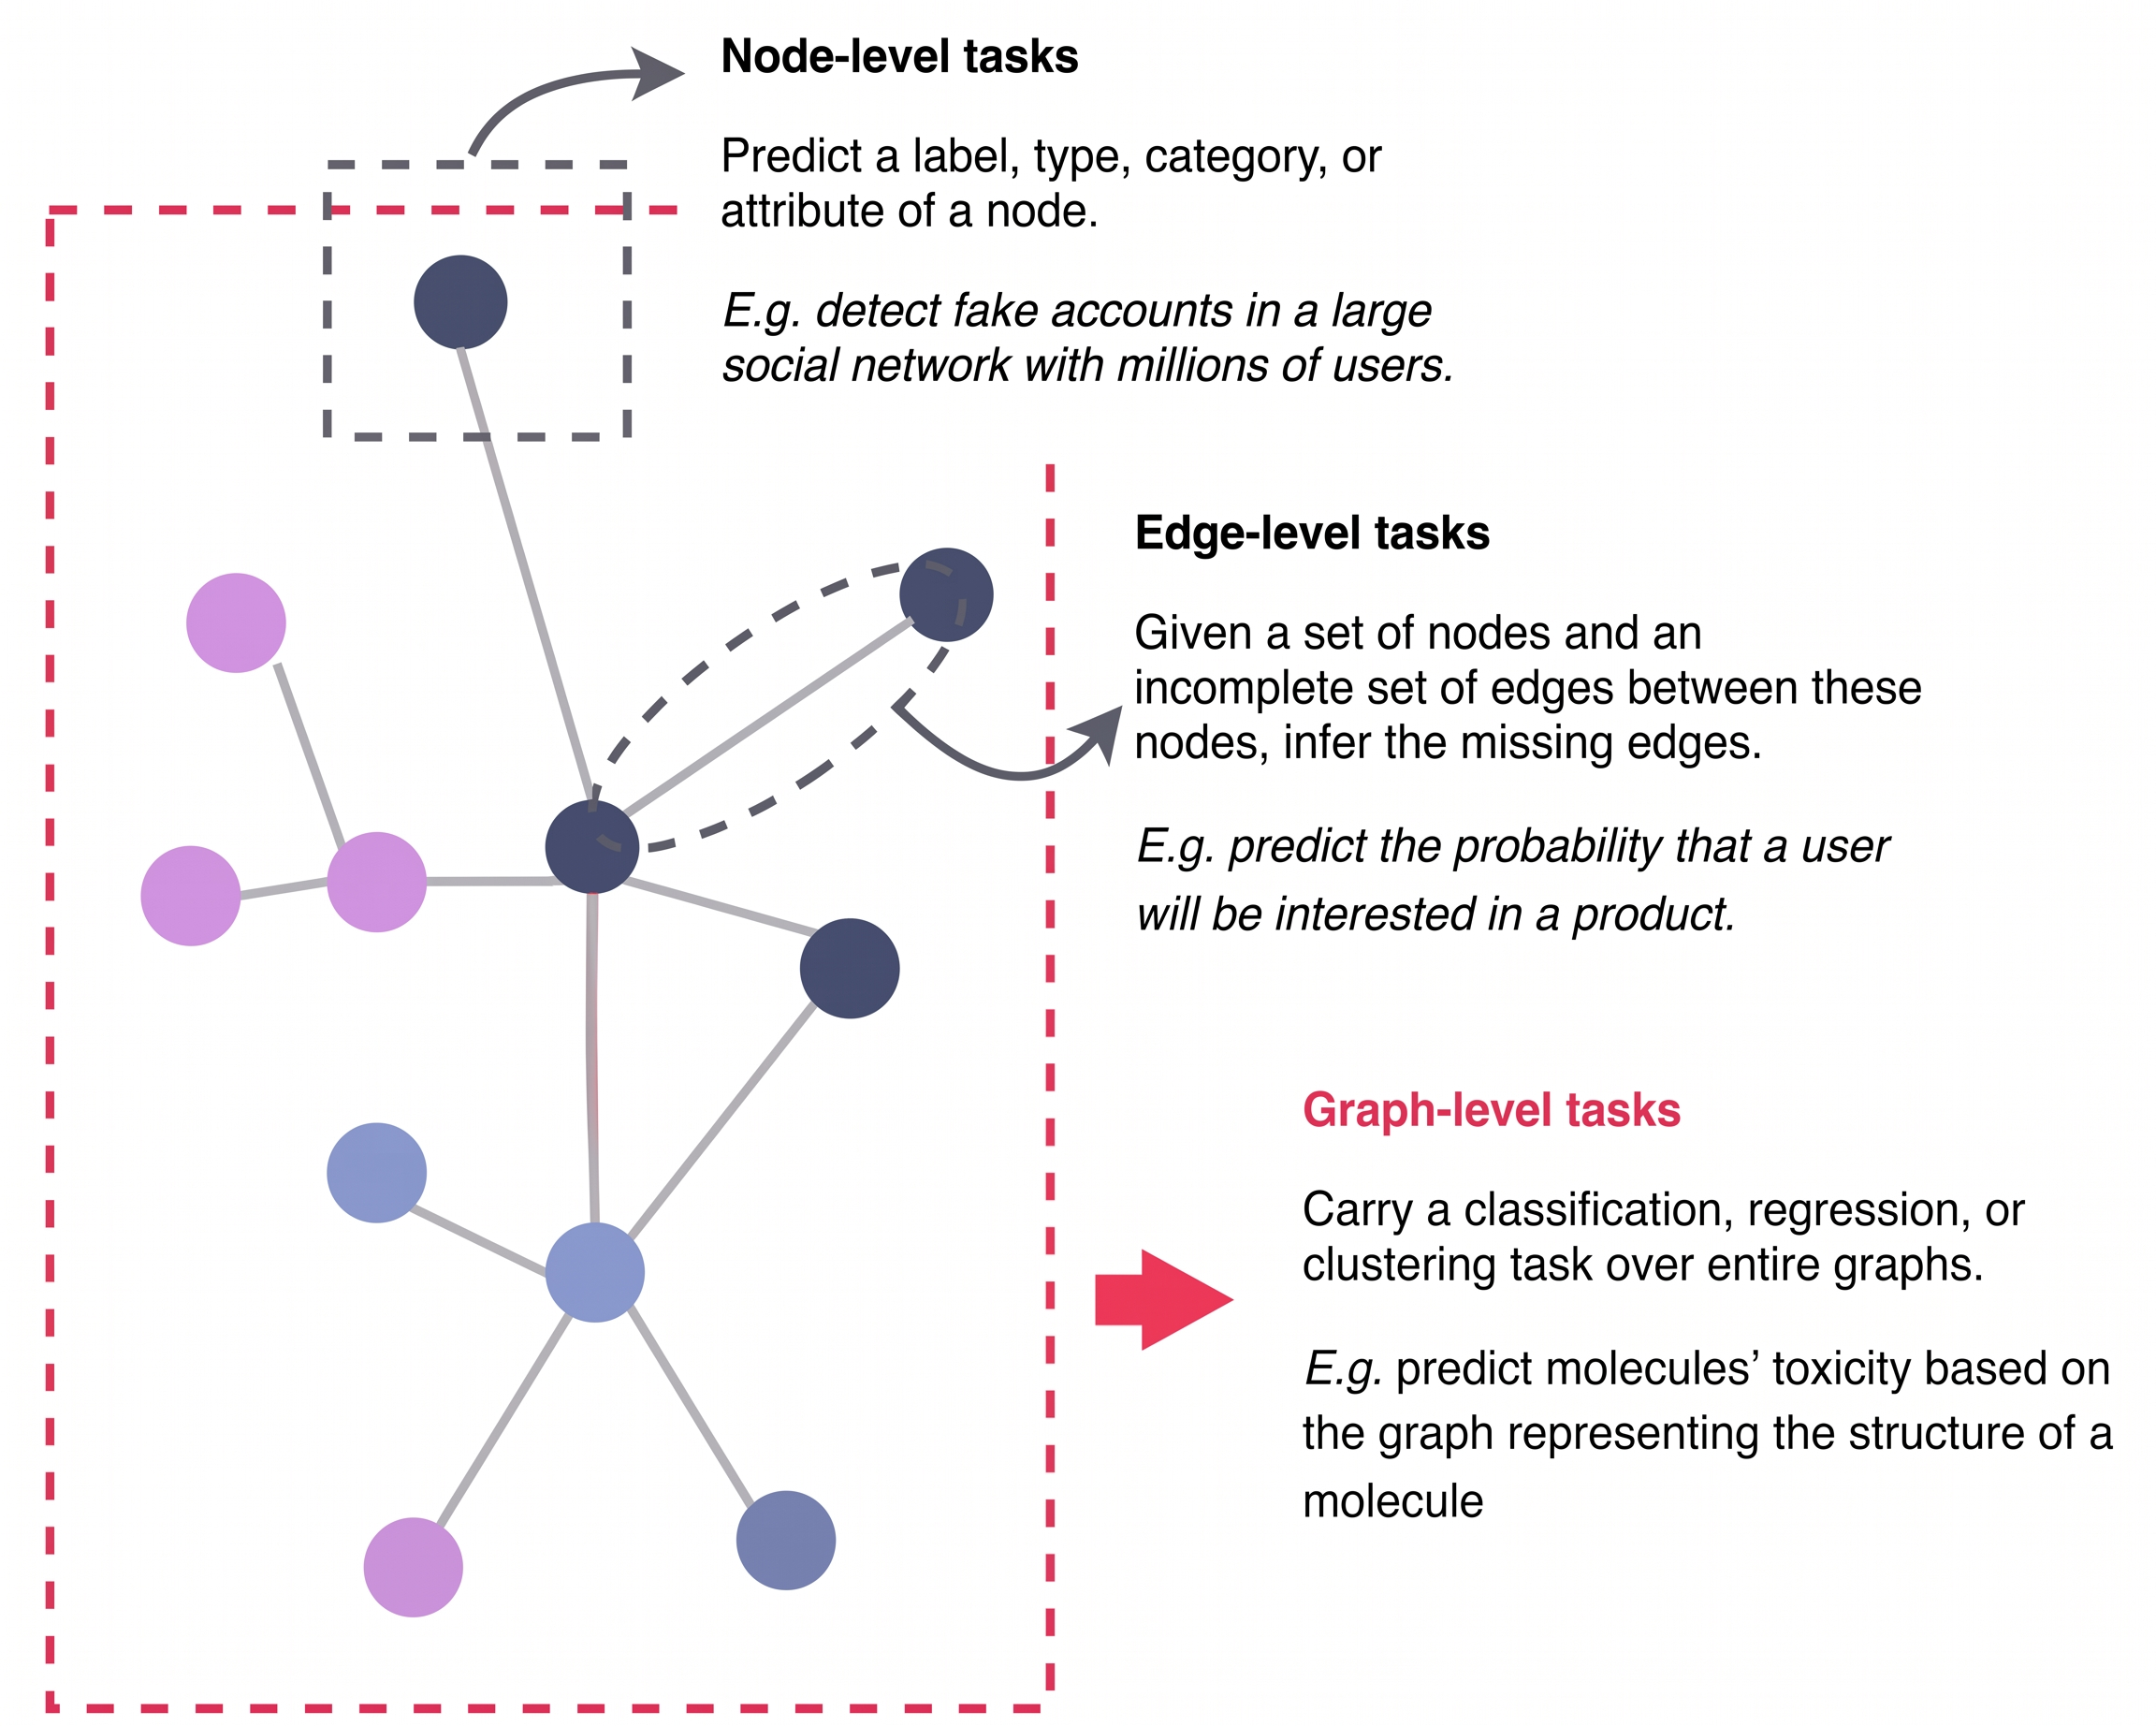
\includegraphics[width=0.45\linewidth]{figuresML/lesson_ml_5_pag_36.png}
\end{center}

\subsection{Building a GNN: Message Passing}
To solve these tasks, the GNN must learn new, richer representations for the nodes, edges, and global state. Just as a CNN extracts hierarchical features through successive convolutional layers, a GNN creates new features by mapping inputs to a high-dimensional latent space and iterating updates across the graph in a process called \textbf{Message Passing}. The mathematical logic follows a sequence of specific operations:

\textbf{1. The Embedding Phase:}
The raw input data typically resides in a physical space $X$, where features might represent concrete quantities like spatial coordinates or velocities. Let ${x_i}$ be the input vector of the node $v_i$ (e.g position, velocity, mass of a celestial body if your graph is representing an astrophysical system). Embedding consists in mapping ${x_i}$ (the physical data) into a higher dimensional vector 
\begin{equation}
    {h_i}=\phi_{\text{EMB}}({x_i})
\end{equation} 
that lies in a latent non-physical space $H$. ${h_i}$ is the so called \textbf{hidden} or \textbf{latent representation} of the node. Crucially, since the same embedding function (which is effectively an embedding neural network) is run over all the nodes, then permutation equivariance is preserved, just like a shared kernel assures translation equivariance for CNNs. 

\textbf{2. The Message Passing Mechanism:}
Once embedded in the high-dimensional latent space, the network updates each node's representation by letting it exchange information with its neighbors. This is the core of message passing, which can be broken down into generating messages, aggregating them, and updating the nodes:

\begin{itemize}
    \item \textbf{Edge Update (Message Generation):} First, information must be passed along the connections. In the absolute simplest scenario, the message on an edge connecting a sender to a receiver could just be a direct copy of the sender's latent vector. More generally, an edge neural network $\phi^e$ computes a message ${e}'_k$ based on the current edge features, the latent vectors of connected nodes, and potentially the global state ${u}$ of the network:
    \begin{equation}
        {e}'_k = \phi^e({e}_k, {h}_{r_k}, {h}_{s_k}, {u})
    \end{equation}
    \item \textbf{Aggregation:} A single node may receive multiple messages from various neighbors, since they might be connected to more than one edges. To process them, the network uses an \textbf{aggregator}, which is a permutation-invariant \textbf{pooling function} $\rho^{e \to v}$ (such as an element-wise sum, a max or a mean). This step effectively compresses the set of incoming message vectors ($E'_i$) into a single unified vector $\bar{{e}}'_i$ of the same dimensionality:
    \begin{equation}
        \bar{{e}}'_i = \rho^{e \to v}(E'_i)
    \end{equation}
    \item \textbf{Node Update:} The node must now synthesize its own current state with the summarized information from its neighbors. A node neural network $\phi^v$ takes the aggregated message $\bar{{e}}'_i$ and the node's current state ${h}_i$ to output the newly updated latent state ${h}'_i$:
    \begin{equation}\label{eq:node_update}
        {h}'_i = \phi^v(\bar{{e}}'_i, {h}_i, {u})
    \end{equation}
\end{itemize}
With that said, why do we need the higher dimensional latent space? \textit{Couldn't we have done it directly with the ${x_i}$ vectors?} The answer lies in the network's capacity to learn complex correlations and structural patterns. Raw physical features often reside in a low-dimensional space and possess heterogeneous units, making direct aggregation mathematically and physically inconsistent. By embedding $X$ into a higher-dimensional latent space, we provide the neural network with the necessary degrees of freedom to unravel non-linear relationships between a node and its neighborhood. Furthermore, in this abstract space, the message passing mechanism can safely aggregate information, combining learned representations rather than incompatible physical quantities and allowing the GNN to effectively cluster nodes based on task-specific similarities. In other words, by iterating this message passing procedure multiple times, nodes gather information from increasingly distant regions of the graph and, after training, nodes with similar relational roles or features will naturally cluster in similar regions of the latent space.

\textbf{3. Global Update (Optional):}
Finally, if the task requires an understanding of the entire system (a graph-level task), a global state can be updated. All updated edges ($E'$) and nodes ($V'$) are pooled into summary vectors:
\begin{align}
    \bar{{e}}' &= \rho^{e \to u}(E') \\
    \bar{{v}}' &= \rho^{v \to u}(V')
\end{align}
A global neural network $\phi^u$ then generates the updated global state ${u}'$:
\begin{equation}
    {u}' = \phi^u(\bar{{e}}', \bar{{v}}', {u})
\end{equation}

\subsection{Information propagation}
By applying the message passing operation multiple times, information flows across the graph. If we define $m$ as the number of message passing iterations, at $m=0$, a node only possesses its initial features. After $m=1$, a node incorporates information from its immediate neighbors. After $m=2$, the node updated representation inherently includes data from nodes two hops away, effectively increasing the receptive field of the network, as represented below. 
\begin{center}
    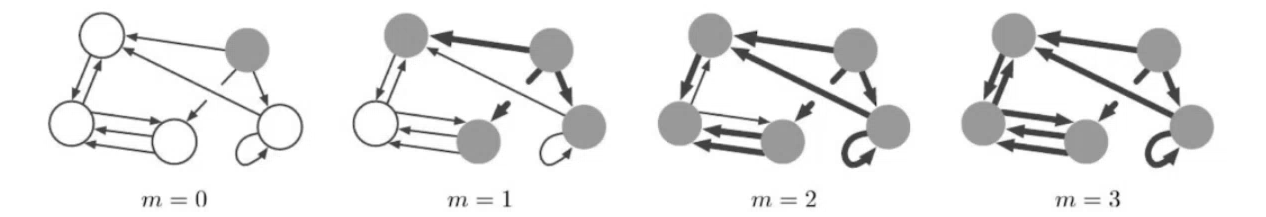
\includegraphics[width=0.8\linewidth]{figuresML/lesson_ml_5_pag_42.png}
\end{center}

\hrulefill

\textbf{Note:} Even though we will not treat them directly, it is worth mentioning the existence of so-called \textbf{heterogeneous graphs}. As shown in the previous diagram, two vertices can have more than one connection in the same direction. This implies that the edge will have two different hidden representations to transmit to the vertices. In practice, this means that the GNN operates as if there were two parallel graphs communicating in different ways. For instance, imagining that the vertices represent private users and companies, and that the algorithm is being used for market research, we might need to update the vertices belonging to the two categories differently. We will not go any further into this topic given its still limited applications in physics.

\hrulefill

Take a look at the following figure. The general algorithm described previously represents the most general possible form of a GNN, but message passing can be implemented in a variety of different ways depending on our specific needs. If, in our 3-body example, we only needed to compute the trajectory of body 3, it would make no sense to implement the updating of the global attributes. In the figure, we can observe different types of GNNs and message passing paradigms. Notice how a Deep-Set is essentially just a GNN without the edges.

\begin{center}
    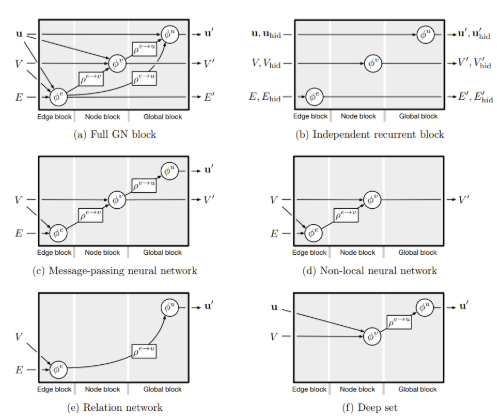
\includegraphics[width=0.7\linewidth]{figuresML/lesson_ml_5a_pag_15}
\end{center}


If the number of message passing steps is too large, or if the graph is fully connected without caution, the \textit{distinct signals from distant nodes can become severely diluted}. Therefore, choosing the correct graph connectivity (which is really an hyperparameter of the network, e.g., using $k$-NN) is essential to ensure the network receives direct and meaningful information. \\
You can find much more on the topic of GNNs in the following review article: \url{https://arxiv.org/abs/1806.01261}.

\subsection{Designing the Loss Function}
As we discussed in the previous sections, GNNs are incredibly versatile because they can handle tasks at the node, edge, and graph levels. But how do we actually train such a multi-faceted network? The answer is that you have total freedom to design a loss function tailored specifically to your physical problem.

Let's consider a practical example from High Energy Physics. When a quark is produced in a collider, it cannot exist in isolation due to the strong nuclear force; instead, it generates a "spray" of multiple particles. We can enclose this entire system in a "box" and represent it as a graph, where the input features are the kinematic properties (e.g., 4-momentum vectors) of the individual particles. If our main goal is a graph-level task (such as determining whether the original parent particle flew a certain distance before decaying or not) we are looking at a global classification problem. The GNN will embed the initial features, perform message passing to update the hidden representations, and finally apply a pooling function to extract a global vector $u'$. Passing $u'$ through MLP yields an output probability. We can then compute a standard \textit{graph-level loss} $\mathcal{L}_{graph}$ as a binary cross entropy.

However, what if we also want to extract local information? Suppose our simulation tells us that one specific particle in the jet is "special" (e.g., it carries a specific physical signature), and we want our network to accurately identify it. We can compute a \textit{node-level loss}, $\mathcal{L}_{node}$, by evaluating the output of the individual node representations.\\
Similarly, returning to our planetary example, if we wanted the network to predict the exact Newtonian force between pairs of planets, we would need to evaluate an \textit{edge-level loss}, $\mathcal{L}_{edge}$, working directly on the edge representations.

The true power of GNNs lies in the fact that these objectives are not mutually exclusive. If your problem requires it, \textit{you can train the network to solve all these tasks simultaneously by simply summing the individual loss components}:
\begin{equation}
    \mathcal{L}_{tot} = \mathcal{L}_{graph} + \mathcal{L}_{node} + \mathcal{L}_{edge}
\end{equation}
By doing so, the gradients backpropagating through the network will optimize the shared embedding and message passing layers to capture both the macroscopic properties of the system and the microscopic details of its individual constituents.

\subsection{Examples of application of GNNs}

\textbf{LHC Jet Tagging} \\
At the LHC, algorithms must quickly determine the origin of particle jets (e.g., identifying if a jet originated from a bottom quark, charm quark, or light quark). Because jets are point clouds, GNN architectures like CMS's \textit{ParticleNet} and ATLAS's \textit{GN1/GN2} have superseded older sequence-based models (like RNNs) and CNNs. These graph networks achieve dramatic improvements, such as a $\sim 5\times$ better background rejection rate when isolating specific decay channels.

\textbf{Global Weather Forecasting}\\
GNNs excel beyond particle physics. Google DeepMind \textit{GraphCast} models the Earth's atmosphere as a simultaneous multi-mesh graph to perform global weather forecasting. By passing messages across this massive spherical grid, it achieves predictions with similar or better accuracy than state of the art high-resolution numerical simulations (HRES) while operating significantly faster.

\subsection{Advanced Concepts: Attention Mechanisms and Dynamic Topologies}\label{sec:intro_att_mech}
While standard Message Passing Neural Networks are incredibly powerful, they traditionally treat the graph's connectivity as an \textit{a priori} hyperparameter. Furthermore, they update node representations without altering the underlying graph structure, which means that the number of nodes and edges remains strictly constant throughout the process. However, modern research and advanced physics applications often require much more flexible architectures.

Instead of hard-coding which nodes are connected using a binary incidence matrix (where elements are purely $1$ for an existing edge and $0$ for no edge), we can initialize a fully connected graph where everything is connected to everything. The goal then becomes to let the network itself learn the \textit{intent} or importance of each passing message. By promoting the binary matrix entries to continuous real numbers, the network dynamically assigns a higher weight to crucial messages and a lower weight to irrelevant ones. This self-learning of message importance is known as the \textbf{Attention Mechanism}. Instead of relying on a human-defined connectivity hyperparameter, the network becomes "attentive" to the specific connections that matter most for the given task. For example, this exact principle is at the very heart of Large Language Models (LLMs), where the network learns the relational importance between different words in a matrix representation of a sentence. We will see this in more detail in Sec. \ref{sec:transformers}.

Moreover, a standard GNN falls short when the task requires mapping an input graph of cardinality $M$ to an output of cardinality $N$, especially when $M \gg N$. A classic example in High Energy Physics is particle tracking: a small number of generated particles (cardinality $N$) might leave dozens of scattered hits (cardinality $M$) across different detector layers. A standard message passing block cannot intuitively reduce these $M$ reconstructed hits back to the $N$ original particles because it preserves the graph's initial dimensions.

To bypass this limitation, researchers are exploring generalized structures like \textbf{hypergraphs}, where hyperedges can connect multiple nodes simultaneously. Another highly effective, state of the art technique is \textbf{Object Condensation}. In this approach, the GNN maps the input nodes into the latent representation space, where we mathematically define interactive potentials. For example, we can introduce a "spring-like" attractive potential that pulls together latent objects belonging to the same physical source, alongside a repulsive potential for background noise or distinct particles. By minimizing this defined potential, the calculation naturally becomes the neural network's loss function, allowing the model to cluster relevant objects together and dynamically reconstruct the original particle sources.

\begin{comment}
\subsection{Advanced Concepts: Set-to-Set Problems and Attention}
While standard GNNs are extremely powerful, they are restricted to updating features without altering the underlying graph structure (the number of nodes and edges remains fixed). In complex tasks like particle tracking, where a network must map thousands of raw detector hits (cardinality $M$) to a handful of actual particle trajectories (cardinality $N$), a simple node update fails because $M \gg N$. 

To solve this, researchers use generalized structures like \textbf{hypergraphs} or a technique called \textbf{object condensation}. In object condensation, the GNN maps nodes into a latent space and defines artificial potentials. For example, a "spring-like" attractive potential pulls together nodes (hits) generated by the same source particle, while a repulsive potential pushes background noise away. Minimizing this potential natively clusters the graph, organically performing instance segmentation.

Another advanced approach to bypass hard-coded connectivity is the \textbf{Attention Mechanism}. Instead of relying on a binary incidence matrix ($1$ for connected, $0$ for not connected), we start with a fully connected graph and promote the connections to continuous real numbers. The neural network dynamically learns to assign weights to these edges, effectively deciding which messages are most important for the task. This self-learning of message importance forms the backbone of modern Transformer models.


\subsection{Practical Exercise: EdgeConv in PyTorch Geometric}
To solidify these concepts, the assignment uses the \texttt{PyTorch Geometric} library to classify point clouds as either circles or rectangles. Unlike standard images, you are provided only with $N$ un-ordered $(x,y)$ coordinates. 

Since the points lack edges, you must build the graph topology dynamically by computing the $k$-Nearest Neighbors ($k=10$). Once the graph is established, you will implement an \textbf{EdgeConv} layer. In this specific architecture, the edge message is generated by passing both the node's position and the relative distance vector between the two connected nodes through a trainable MLP, successfully extracting geometric features from an unstructured point cloud.
\end{comment}
\section{Hands-on examples for Graph Neural Networks}

This section will contain two Notebooks that will be crucial in comprehending how GNNs are implemented.

The first exercise consists of creating a Graph Neural Network (GNN) using \texttt{torch\_geometric} to recognize whether an image, represented as a point cloud, contains a rectangle or a circle. In the second one, you will tackle a more complex custom graph problem using the Deep Graph Library (\texttt{dgl}) to build an object condensation model. 

Here are the links to the Colab Notebooks:
\begin{enumerate}
    \item \url{https://colab.research.google.com/drive/1uz9OdJsD_RcDMlxCWqvN7rPXGWk-KZ1t?usp=sharing}
    \item \url{https://colab.research.google.com/drive/1j-rmo5-ro7LkosqiKpojPYlrqdgYzfmr?usp=sharing}
\end{enumerate}

Instead of using \texttt{keras}, we will be working with the \texttt{PyTorch} library. The rationale behind this shift is flexibility: especially within the high-energy physics community, researchers frequently need to build custom architectures that deviate from standard, built-in models. PyTorch offers the granular control required to implement these novel, physics-informed architectures, making it the standard tool for professional applications. You will find the necessary documentation here: \url{https://docs.pytorch.org/docs/main/}.

Since I have to start a new page in order to input the Notebook in my LaTeX file, here is a photo of all the Slam winners of the year 2000. In order: Andre Agassi at the 2000 Australian Open (\textit{upper left}), Gustavo Kuerten at the 2000 Roland Garros (\textit{upper right}), Pete Sampras at the 2000 Wimbledon with the runner-up Pat Rafter (\textit{bottom left}) and Marat Safin at the 2000 US Open (\textit{bottom right}).  

\begin{center}
    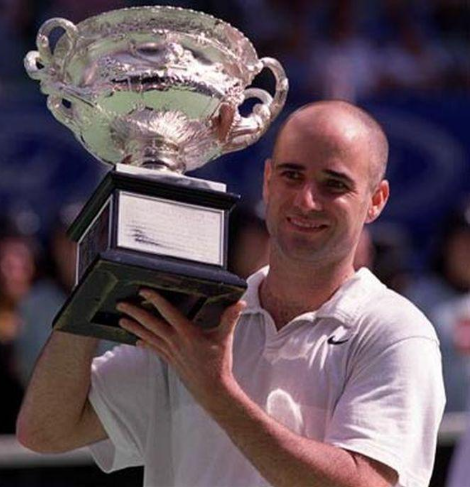
\includegraphics[width=0.3\textwidth]{figuresML/2000_agassi}
    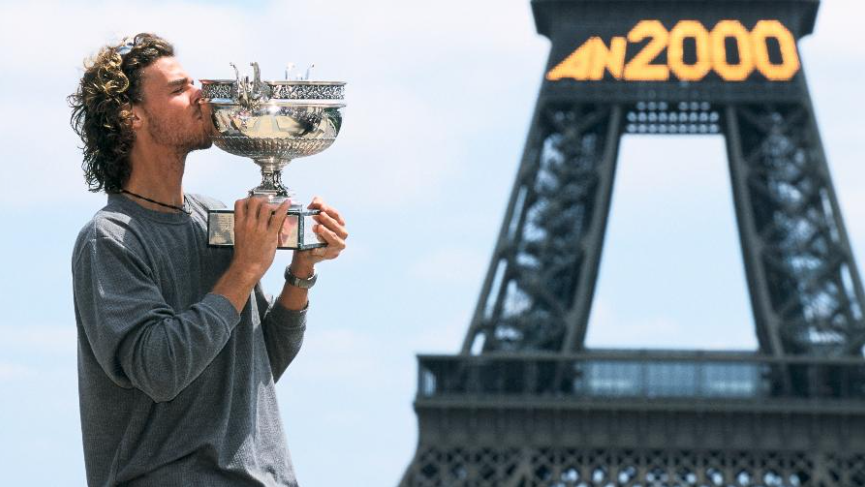
\includegraphics[width=0.5\textwidth]{figuresML/2000_kuarten}
    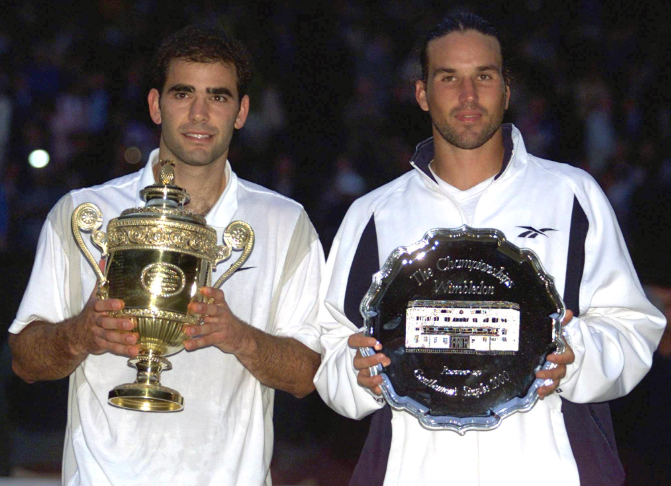
\includegraphics[width=0.5\textwidth]{figuresML/2000_sampras}
    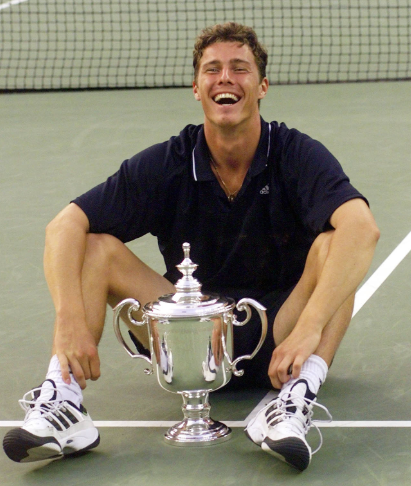
\includegraphics[width=0.3\textwidth]{figuresML/2000_safin}
\end{center}

%\includepdf[pages=-, pagecommand={\thispagestyle{plain}}]{lezioni/d_ML6a_SOL.pdf} 
%ML_5 nel mio colab

%\includepdf[pages=-, pagecommand={\thispagestyle{plain}}]{lezioni/d_ML6b_SOL.pdf}
%ML_9 nel mio colab

%\end{comment}


% -------------------------------------------------------------------
% PART IV: Machine Learning (Advanced)
% -------------------------------------------------------------------
\chapter[Advanced concepts in Machine Learning]{Advanced concepts in Machine Learning \\[0.5ex] \large \textit{(Prof. Di Bello, Prof. Rizzi)}}

%\begin{comment}
\section{Advanced concepts for VAEs with hands-on example}

This section marks the beginning of the advanced module in Machine Learning, which will cover several cutting-edge topics. We will begin with Generative Modeling, specifically exploring in more detail Variational Autoencoders and Normalizing Flows, which are currently among the most powerful and trendy generative techniques. We will then transition into advanced concepts for Graph Neural Networks and Transformer models with some realistic use cases.

\subsection{Recap of standard autoencoders}
To deeply understand modern generative models, let us first revisit the standard autoencoder. \\
An autoencoder consists of two distinct MLPs, as shown in figure:
\begin{itemize}
    \item[-] The encoder ($g_\phi$): Parameterized by weights $\phi$, it translates the original high-dimensional input $x$ (like an unwrapped $32 \times 32$ image) into a low-dimensional latent representation $z$.
    \item[-] The decoder ($f_\theta$): Parameterized by weights $\theta$, it takes the compressed code $z$ and attempts to reconstruct the original high-dimensional data as $x'$.
\end{itemize}

\begin{center}
    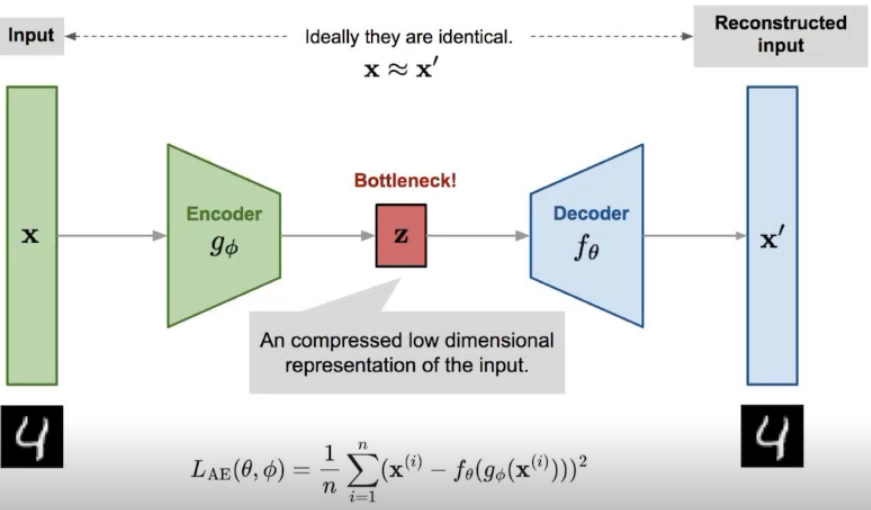
\includegraphics[width=0.6\textwidth]{figuresML_adv/lesson_ml_adv_1_pag_2.png}
\end{center}

An autoencoder is a neural network trained in an entirely unsupervised manner, since there are no explicit labels (e.g., "this is a dog" or "this is a cat"). The goal of the network is simply to reproduce its input, outputting a vector $x'$ as similar as possible to the input $x$. Due to the dimensionality reduction step, the output should looked "blurred" (if you think about an image) with respect to the input.

The critical feature of this architecture is the bottleneck: by forcing the data through a latent space $Z$ with a much smaller dimensionality than $X$, the network cannot simply learn the identity function, but it is forced to learn an efficient compression scheme, extracting the most vital underlying features of the data. The network is trained by minimizing a reconstruction loss, typically the mean squared error, between the input and the output:
\begin{equation}
    \mathcal{L}_{AE}(\theta, \phi) = \frac{1}{n} \sum_{i=1}^n \left( x^{(i)} - f_\theta(g_\phi(x^{(i)})) \right)^2
\end{equation}

While standard autoencoders are excellent for tasks like data compression or anomaly detection (e.g., fraud detection in finance), they \textit{cannot be used for generation}, because the latent space $Z$ is entirely unregularized. The encoder maps inputs to specific, isolated discrete points in the latent space, and if we arbitrarily sample a random point in an empty region of this latent space and pass it to the decoder, the network will output meaningless noise, as it has never learned what that empty space represents \footnote{This is actually the reason why autoencoders are useful for anomaly detection: a random point in the $Z$ space will be easily recognizable since it will most likely be projected far away from know clustered regions in the $X$ space by the network.}. 

\subsection{Variational Autoencoders in depth}

To transform the standard autoencoder into a true generative model, we must introduce stochasticity and regularize the latent space. We no longer want to map the input to a single, deterministic point; instead, we want to map it to a \textit{probability distribution}. This is the foundational concept of the Variational Autoencoder (VAE) and the very meaning behind the word "variational": running the inference process twice on the same input will yield similar, but not perfectly identical, outputs.

In a VAE, we define the problem using precise probabilistic language:
\begin{itemize}
    \item[-] $\mathbf{p_\theta(x)}$: the true likelihood (probability density function) of the training data, which we ultimately want to maximize. The parameters $\theta$ represent the network weights governing the generation of the data.
    \item[-] $\mathbf{q_\phi(z|x)}$: the encoder. It approximates the intractable true posterior $p_\theta(z|x)$ by learning to model a conditional Gaussian distribution given the input $x$. The parameters $\phi$ represent the learnable weights of this encoder network.
    \item[-] $\mathbf{p_\theta(x|z)}$: the decoder. It models the likelihood distribution of the data $x$ given the sampled latent variable $z$. 
    \item[-] $\mathbf{p(z)}$: the prior. This is the target distribution we want our latent space to resemble, that is completely independent from the data $x$. We can then decide freely for $p(z)$ to be a standard normal distribution $\mathcal{N}(0, 1)$.
\end{itemize}

\begin{center}
    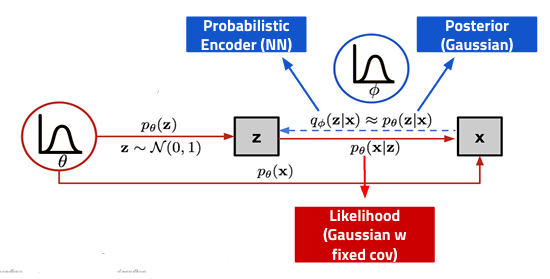
\includegraphics[width=0.75\textwidth]{figuresML_adv/lesson_ml_adv_1_pag_3.png}
\end{center}

Practically speaking, how do we implement this distribution mapping? Instead of a standard Multi-Layer Perceptron (MLP) outputting a single vector $z$, the encoder network $q_\phi$ is designed to output two distinct vectors: a mean ($\mu$) and a standard deviation ($\sigma$). For instance, if we choose a 2-dimensional latent space to easily visualize the data, the network will output two mean values ($\mu_1, \mu_2$) and two standard deviations ($\sigma_1, \sigma_2$). We deliberately assume that the covariance matrix of this multi-dimensional Gaussian is completely diagonal for simplicity. 
Therefore, an input image is no longer encoded as a single dot in the latent space, but rather as a 2D Gaussian curve characterized by the learned $\mu$ and $\sigma$.

To generate the output, we must sample a latent vector $z$ from this newly defined Gaussian distribution and pass it to the decoder. However, this introduces a critical mathematical roadblock during training: the sampling process itself is fundamentally stochastic, meaning it has no derivative. In other words, $\dfrac{\partial z}{\partial \mu}$ and $\dfrac{\partial z}{\partial \sigma}$ cannot be computed if $\mu$ and $\sigma$ are sampled stochastically. If we cannot compute the derivative of the sampling step, then we cannot backpropagate the error through the network to update the encoder weights $\phi$.

To solve this, we employ a clever mathematical workaround known as the \textbf{reparameterization trick}. Instead of sampling directly from the parameterized Gaussian, we express the latent variable as:
\begin{equation}
    z = \mu_\phi(x) + \sigma_\phi(x) \times \epsilon
\end{equation}
where $\epsilon \sim \mathcal{N}(0, I)$ is a small variation sampled from a standard normal distribution. By doing this, we isolate the stochasticity entirely within the independent variable $\epsilon$ and we get
\begin{equation*}
    \dfrac{\partial z}{\partial \mu_{\phi}}=1 \quad, \quad \dfrac{\partial z}{\partial \sigma_{\phi}}=\epsilon
\end{equation*}
The nodes computing $\mu$ and $\sigma$ remain deterministic, allowing the gradients to flow smoothly backward through the network during the optimization process.

\subsection{The Evidence Lower Bound (ELBO) and VAE Loss Function}

Because the VAE is a probabilistic model, its objective function requires a paradigm shift: we must rethink the concept of a loss function as the maximization of a likelihood. 

\subsubsection{Loss Functional as a Likelihood}
To understand this connection, let us recall a standard laboratory physics problem: finding the line of best fit $Y = mX + q$. When we perform this fit by minimizing the $\chi^2$, we are implicitly assuming that the probability density function of our experimental events is Gaussian. The likelihood $\mathcal{L}$ of observing all our data points is the product of these individual Gaussian probabilities:
\begin{equation*}
    \mathcal{L} = \prod_i \text{Gauss}(Y_i - (mX_i + q); \sigma_i)
\end{equation*}
To simplify the mathematics, we take the negative logarithm of the likelihood. Because the logarithm of an exponential leaves only the argument, we obtain:
\begin{equation*}
    -\log \mathcal{L} \sim \sum_i \frac{(Y_i - (mX_i + q))^2}{\sigma_i^2} = \chi^2
\end{equation*}
Finding the optimal parameters $m$ and $q$ by minimizing the $\chi^2$ is therefore mathematically identical to maximizing the likelihood of the data.

This exact logic applies to neural networks. Suppose we have a MLP performing a regression task, learning a function $f_\phi(x)$ parameterized by weights $\phi$. If we assume the output follows a Gaussian distribution with a constant variance $\sigma_i^2 = \text{const}$, the negative log-likelihood becomes:
\begin{equation*}
    -\log \mathcal{L} \sim \sum_i (Y_i - f_\phi(X_i))^2
\end{equation*}
This demonstrates that minimizing the MSE is mathematically equivalent to maximizing a Gaussian likelihood. Similarly, if our data follows a Bernoulli distribution (e.g. binary variables where an event either happens or not), taking the negative log-likelihood of the Bernoulli distribution mathematically yields the binary cross-entropy loss (try to prove it on your own). In short: \textit{every loss function is intrinsically a likelihood}.

\subsubsection{Deriving the ELBO}
In a generative model like a VAE, our primary objective is to maximize the true likelihood of the data, $p_\theta(x)$. However, the true posterior $p_\theta(z|x) = \frac{p_\theta(x,z)}{p_\theta(x)}$ is computationally intractable because calculating $p_\theta(x)$ requires an impossible integration over all possible latent spaces.

To bypass this, we can use a simple but clever trick. We approximate the true posterior using our encoder $q_\phi(z|x)$, and measure the difference between our approximation and the truth using the Kullback-Leibler divergence in eq. \ref{eq:KL_div}, which by definition is always non-negative:
\begin{equation*}
    D_{KL}(q_\phi(z|x) || p_\theta(z|x)) \ge 0
\end{equation*}
Using Bayes' rule, we can substitute $\log p_\theta(z|x) = \log p_\theta(x,z) - \log p_\theta(x)$ into the definition of the KL divergence:
\begin{equation*}
\begin{aligned}
    0 &\le \mathbb{E}_{q_\phi} [\log q_\phi(z|x) - \log p_\theta(z|x)] \quad \Rightarrow \\
    0 &\le \mathbb{E}_{q_\phi} [\log q_\phi(z|x) - (\log p_\theta(x,z) - \log p_\theta(x))] 
\end{aligned}
\end{equation*}
Because $\log p_\theta(x)$ does not depend on the latent variable $z$, we can extract it directly from the expectation. Rearranging the terms, we arrive at a fundamental inequality:
\begin{equation*}
\begin{aligned}
    0 &\le \mathbb{E}_{q_\phi} [\log q_\phi(z|x) - \log p_\theta(x,z)] + \log p_\theta(x) \quad \Rightarrow \\
    \log p_\theta(x) &\ge \mathbb{E}_{q_\phi} [\log p_\theta(x,z) - \log q_\phi(z|x)] \equiv \text{ELBO}
\end{aligned}
\end{equation*}
This term is called the \textbf{Evidence Lower Bound (ELBO)}. Since we cannot maximize the true log-likelihood directly, we maximize the ELBO instead. Pushing up this lower bound guarantees that we are simultaneously pushing up the true likelihood of our data.

By applying the joint probability identity $\log p_\theta(x,z) = \log p_\theta(x|z) + \log p(z)$, we can expand the ELBO into two highly practical terms:
\begin{equation*}
\begin{aligned}
    \text{ELBO} &= \mathbb{E}_{q_\phi} [\log p_\theta(x|z) + \log p(z) - \log q_\phi(z|x)] \quad \Rightarrow \\
    \text{ELBO} &= \mathbb{E}_{q_\phi} [\log p_\theta(x|z)] - D_{KL}(q_\phi(z|x) || p(z))
\end{aligned}
\end{equation*}
Because standard machine learning optimization minimizes a loss function rather than maximizing an objective, the \textbf{VAE Loss Function} is defined as the negative ELBO:
\begin{equation}
    \mathcal{L}_{VAE}(\theta, \phi; x) = - \mathbb{E}_{q_\phi(z|x)}[\log p_\theta(x|z)] + D_{KL}(q_\phi(z|x) || p(z))
\end{equation}

\subsubsection*{Analyzing the Loss Components}
This loss function elegantly balances two competing forces:

\begin{itemize}
    \item \underline{The reconstruction term}: $- \mathbb{E}_{q_\phi}[\log p_\theta(x|z)]$ \\ This is the negative log-likelihood of our decoder. It heavily penalizes the network if it fails to accurately reconstruct the input $x$ from the sampled latent vector $z$. Following our initial digression, we can formally derive the loss based on the data type:
    \begin{itemize}
        \item For continuous data, we assume a \textit{Gaussian} likelihood. The expression mathematically resolves to the MSE:
        \begin{equation*}
        \begin{aligned}
            p_\theta(x|z) &= \mathcal{N}(x; \hat{x}(z), \sigma^2 I) \quad \Rightarrow \\
            -\log p_\theta(x|z) &= \frac{1}{2\sigma^2} ||x - \hat{x}(z)||^2 + \text{const}
        \end{aligned}
        \end{equation*}
        
        \item For binary data (like MNIST pixels), we assume a \textit{Bernoulli} likelihood. The expression mathematically resolves to the BCE:
        \begin{equation*}
        \begin{aligned}
            p_\theta(x|z) &= \text{Bernoulli}(\hat{x}(z)) \quad \Rightarrow \\
            -\log p_\theta(x|z) &= -\sum_{i=1}^{D} [x_i \log \hat{x}_i + (1 - x_i) \log(1 - \hat{x}_i)]
        \end{aligned}
        \end{equation*}
    \end{itemize}
    
    \item \underline {The KL divergence term}: $D_{KL}(q_\phi(z|x) || p(z))$ \\ This term acts as a spatial regularizer. Geometrically, without this term, the network would map different input classes into distant, isolated clusters in the latent space. Sampling from the empty space between these clusters would produce nonsensical noise. The KL divergence acts like a physical spring, pulling the approximate posterior $q_\phi(z|x)$ toward the standard normal prior $p(z) = \mathcal{N}(0, I)$, forcing the clusters to overlap smoothly and creating a continuous generative space.
    
    Because we explicitly defined both the encoder and the prior as Gaussians, this term is not estimated but can be calculated analytically in a closed form. Let the encoder output be $q(z) = \mathcal{N}(z; \mu, \text{diag}(\sigma^2))$ and the prior be $p(z) = \mathcal{N}(z; 0, I)$. Expanding their log-densities yields:
    \begin{equation*}
    \begin{aligned}
        \log q(z) &= -\frac{1}{2}\sum_{j=1}^{d}\left[\log(2\pi\sigma_j^2) + \frac{(z_j-\mu_j)^2}{\sigma_j^2}\right] \\
        \log p(z) &= -\frac{1}{2}\sum_{j=1}^{d}\left[\log(2\pi) + z_j^2\right]
    \end{aligned}
    \end{equation*}
    By substituting these into the definition $D_{KL}(q||p) = \mathbb{E}_{q}[\log q(z) - \log p(z)]$ and evaluating the expectations (knowing that $\mathbb{E}_q[(z_j-\mu_j)^2] = \sigma_j^2$ and $\mathbb{E}_q[z_j^2] = \mu_j^2 + \sigma_j^2$), all constants cancel out beautifully to leave:
    \begin{equation}
        D_{KL}(q||p) = \frac{1}{2} \sum_{j=1}^{d} \left( \mu_j^2 + \sigma_j^2 - 1 - \log \sigma_j^2 \right)
    \end{equation}
\end{itemize}

\subsection{Advanced hands-on example on VAE}
In the following example, a Variational Autoencoder is used to classify user generated images containing rectangles and circles. Instead of using \texttt{keras}, we will be working with the \texttt{PyTorch} module.
The rationale behind this shift is flexibility: especially within the high energy physics community, researchers frequently need to build custom architectures that deviate from standard, built-in models. PyTorch offers the granular control required to implement these novel, physics-informed architectures, making it the standard tool for professional applications. You will find the necessary documentation here: \url{https://docs.pytorch.org/docs/main/}. 

Since I have to start a new page in order to input the Notebook in my LaTeX file, here is a Federer forehand at the 2006 US Open to occupy the rest of the page.

\begin{center}
    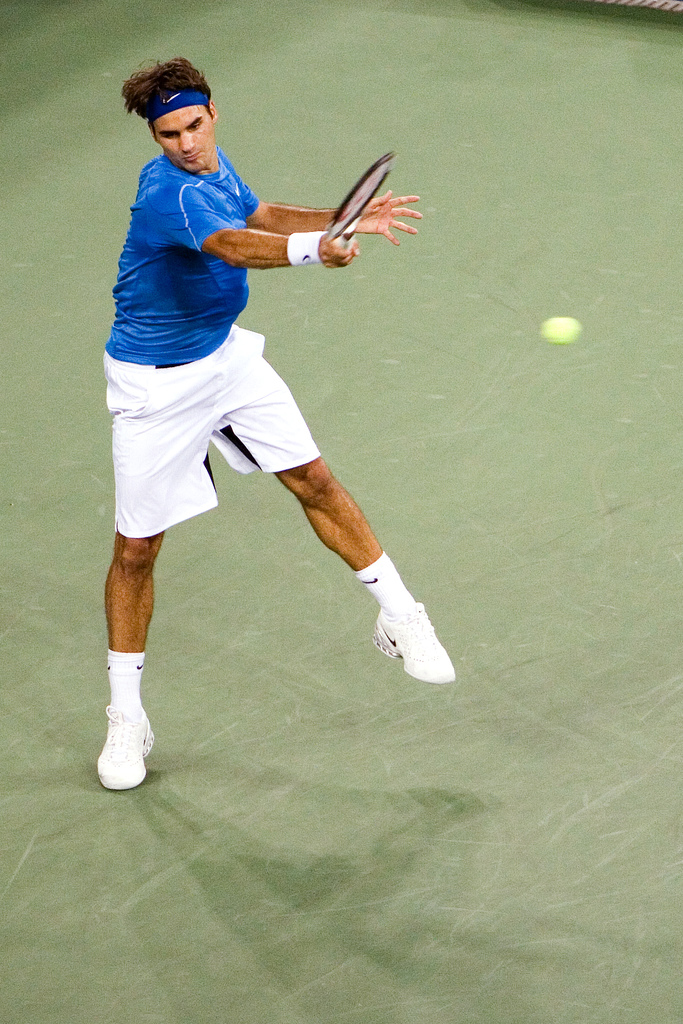
\includegraphics[width=0.25\textwidth]{figuresML/Roger_Federer_US_Open_2006.jpg}
\end{center}

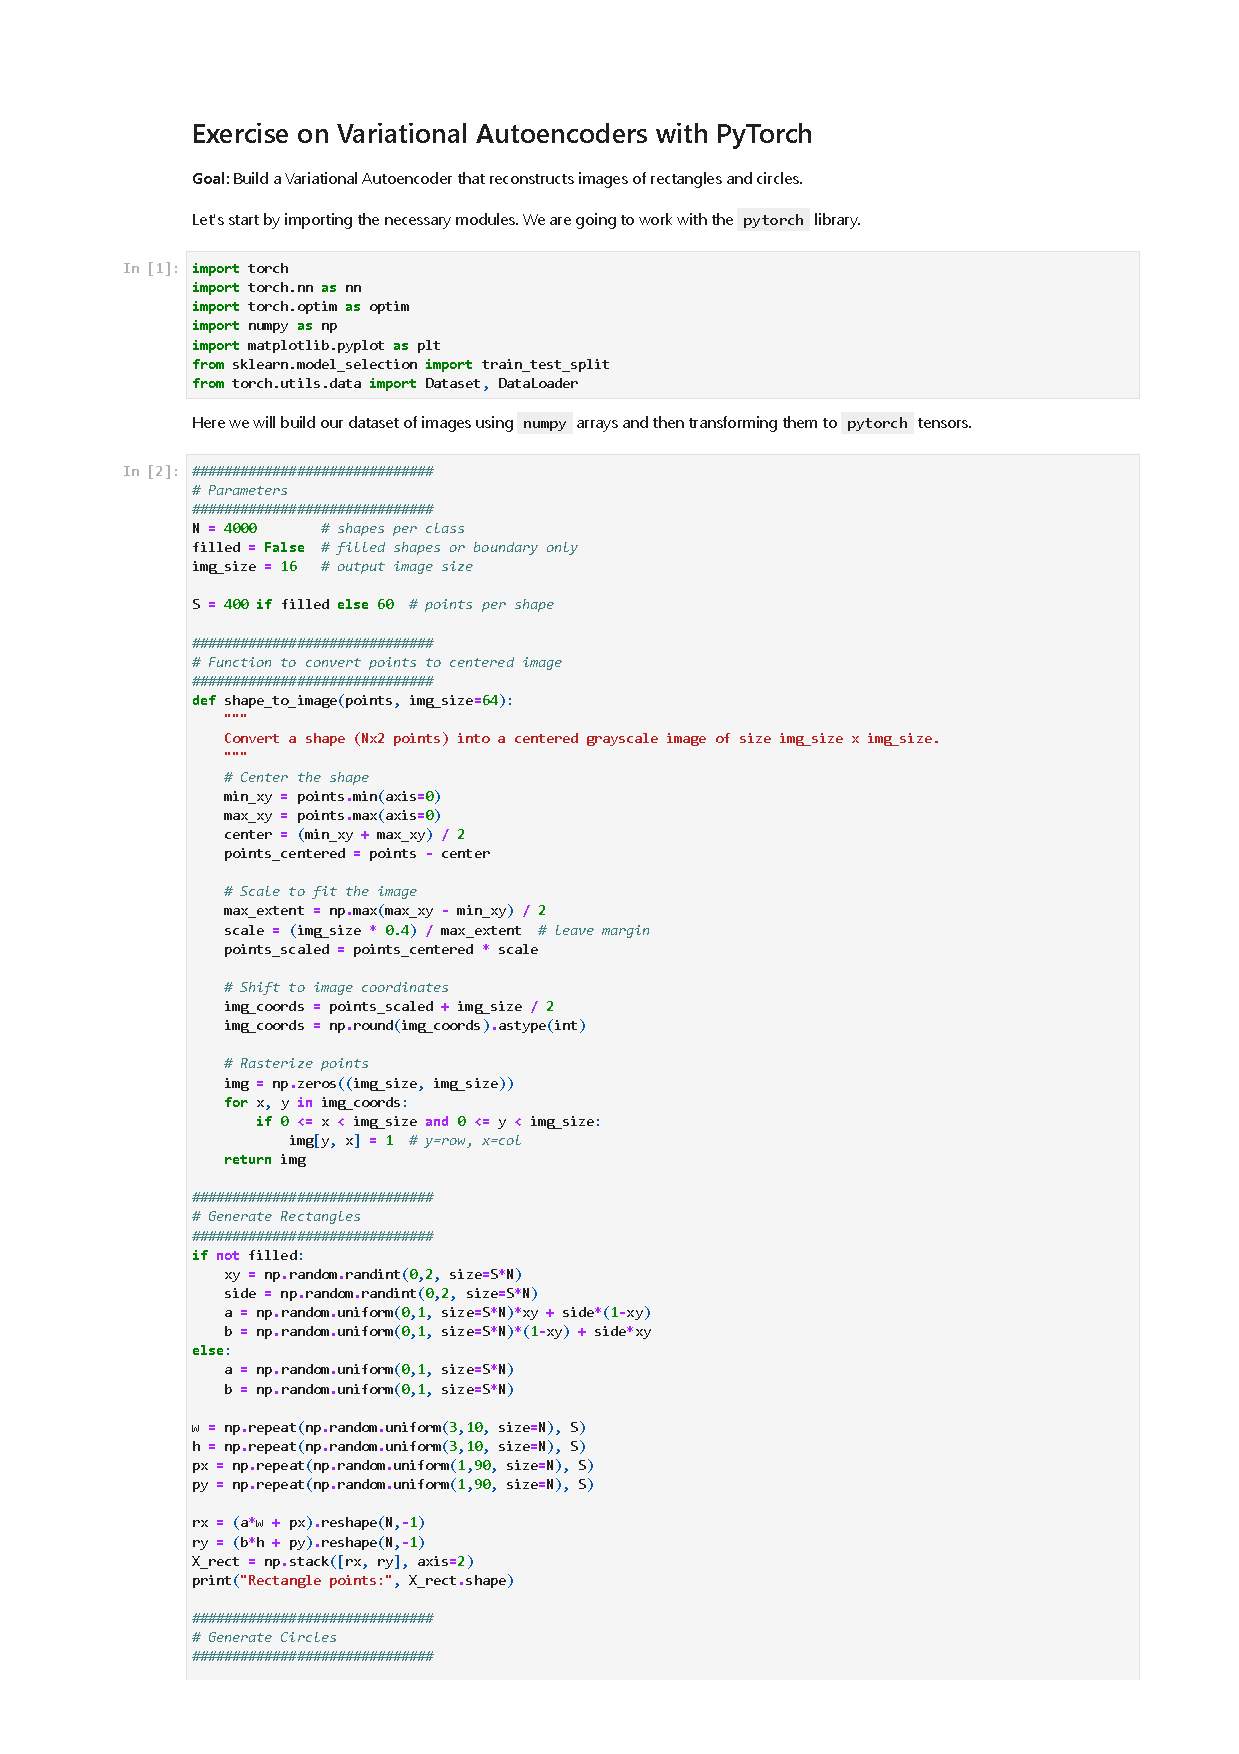
\includepdf[pages=-, pagecommand={\thispagestyle{plain}}]{lezioni/e_ML_adv_1hands_on.pdf} 
% ML_6 nel mio Colab
\section{Convolutional Autoencoders and U-Net}

\subsection{Convolutional Autoencoders (CAEs)}
As said, a Convolutional Neural Network processes structured grid data (like images) using a convolution operation defined by a kernel or filter. By sliding these filters across the image, CNNs naturally extract hierarchical features while drastically reducing the number of parameters compared to dense networks. \\
We can view a standard CNN as a powerful information compressor or encoder. In a classification task, a CNN processes an input image through successive convolutional and pooling layers until the spatial dimensions are severely compressed, finally feeding the extracted feature maps into a neural network (usually a MLP) to output class probabilities. If we remove the final NN classifier, we are left with a purely convolutional feature extractor. What if we try to decode this compressed representation back into the original image space? By attaching a \textit{convolutional decoder} to our \textit{convolutional encoder}, we create a \textbf{Convolutional Autoencoder (CAE)}. 

\begin{center}
    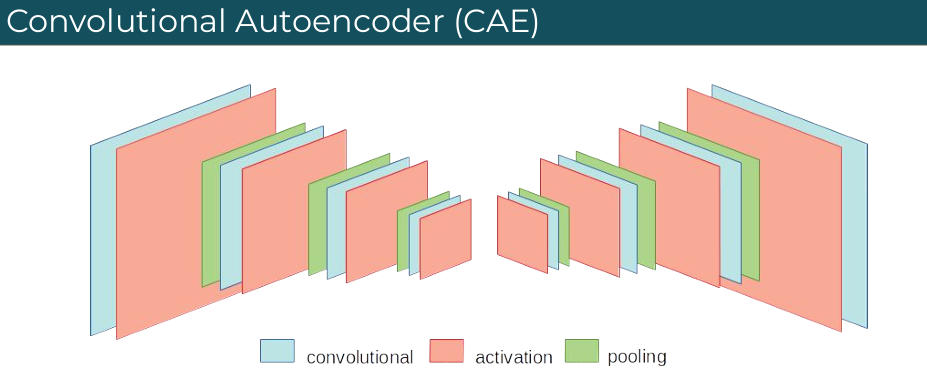
\includegraphics[width=0.75\textwidth]{figuresML_adv/lesson_ml_adv_2_pag_21.png}
\end{center}

\subsection{Upsampling and transposed Convolution in CAE}
In the encoder half of a CAE, pooling operations and strided convolutions are used to downsample the spatial dimensions of the image. That means that the latent space is no longer a simple 1D vector but a set of highly compressed, deep feature maps which constitute the latent representation of the data. To reconstruct the image in the decoder, we must invert this process and increase the spatial resolution of the feature maps.

\begin{figure}[H]
    \begin{minipage}[c]{0.55\textwidth}
        There are two primary ways to increase spatial resolution, as shown in the following figures:
        \begin{enumerate}
            \item \textit{Simple upsampling:} This is a fixed, non-learnable operation. It simply takes a pixel value and repeats it across a larger area. For instance, a $2 \times 2$ grid can be expanded to a $4 \times 4$ grid by duplicating each pixel into a $2 \times 2$ block. 
            \item \textit{Transposed convolution (Deconvolution):} Unlike simple upsampling, transposed convolution is a \textit{learnable} operation. It applies trainable filters to expand the spatial dimensions. For example, a single pixel in the compressed feature map is multiplied by a $2 \times 2$ filter (with a stride of 2), projecting its values into a $2 \times 2$ output grid. Where the projected outputs overlap, their values are summed. This allows the network to actively learn how to optimally reconstruct spatial details.
        \end{enumerate}
    \end{minipage}\hfill
    \begin{minipage}[c]{0.44\textwidth}
        \centering
        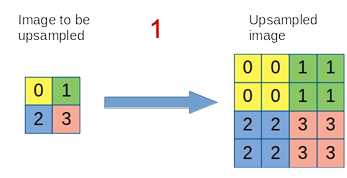
\includegraphics[width=0.85\textwidth]{figuresML_adv/lesson_ml_adv_2_pag_33.png}
        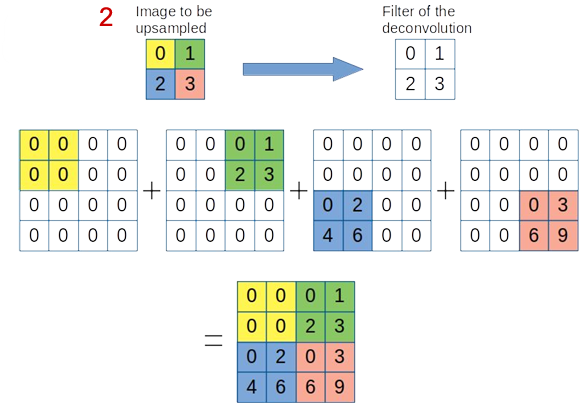
\includegraphics[width=0.85\textwidth]{figuresML_adv/lesson_ml_adv_2_pag_33a.png}
    \end{minipage}
\end{figure}
\vspace{-7.5mm}
With that said, it should be clear that CAEs are incredibly effective for unsupervised feature extraction. For example, take a look at the following study: \url{https://ieeexplore.ieee.org/document/7412749}. Here, Convolutional Sparse Autoencoders (CSAE) (a kind of CAE that introduces a sparsity penalty to force the most neurons to remain inactive for every given input) have been successfully used in medical imaging to extract features for breast density segmentation and mammographic risk scoring. The unsupervised CSAE isolates dense tissue structures without requiring pixel-perfect manual annotations, providing a foundation for subsequent supervised classifiers.

\subsection{Regularization in CNNs: spatial dropout}
Like any deep neural network, if a CAE has an excessively high capacity, it risks overfitting the training data. We must apply regularization techniques such as modifying the cost function with penalties, utilizing data augmentation, or applying batch normalization. 

A common regularization technique for MLPs is dropout, where random neurons are deactivated during training. However, applying standard dropout to CNN makes very little sense: in an image, adjacent pixels are highly correlated, so if you drop a single random pixel, the network can easily bypass the dropout by simply relying on the neighboring pixels, meaning the feature extractors can easily adapt to the change. To properly regularize a CNN, we use \textbf{spatial dropout}, a technique schematically reported in figure: instead of dropping individual random pixels, spatial dropout drops \textit{entire feature maps (channels) at random}. By completely zeroing out an entire filter's output for a given iteration, the network is forced to learn independent, robust feature representations rather than relying on a specific combination of parallel filters.

\begin{center}
    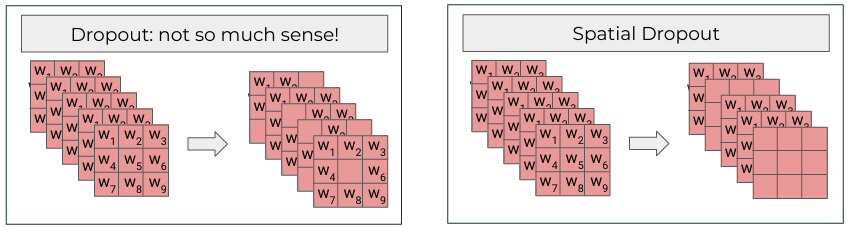
\includegraphics[width=0.85\textwidth]{figuresML_adv/lesson_ml_adv_2_pag_37.png}
\end{center}

\subsection{The U-Net architecture and skip connections}
Standard Convolutional Autoencoders suffer from a critical flaw when applied to highly detailed tasks like segmentation: the bottleneck compresses the image so severely that fine-grained spatial details (exact edges, boundaries, and microscopic structures) are permanently lost. The decoder struggles to reconstruct these sharp details from the low-resolution latent space alone.

To solve this, the \textbf{U-Net} architecture was introduced. U-Net is a fully convolutional neural network (which means it contains zero dense layers) featuring an encoder-decoder structure. It was implemented in 2015 for biomedical image segmentation of various organs, and it can still today be considered the state of the art architecture in its field. Its defining innovation is the use of the so called \textit{long skip connections}. Take a look at its structure in the following figure: as illustrated by the "U" shape of the architecture, the high-resolution feature maps from the early layers of the encoder are passed directly across the network and \textit{concatenated} with the upsampled feature maps in the decoder. 

\begin{center}
    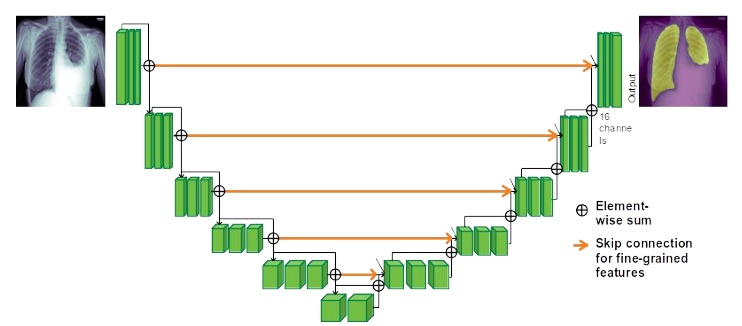
\includegraphics[width=0.85\textwidth]{figuresML_adv/lesson_ml_adv_2_pag_30.png}
\end{center}

We talked about skip connections in Sec. \ref{sec:skip_connections} regarding the ResNet algorithm and its functioning principle. Now let's take it a step further and distinguish between two different types of skip connections:
\begin{itemize}
    \item \textbf{Short Skip Connections} (e.g., ResNet, black lines in the figure above): Use element-wise \textit{addition} between closely grouped layers. Their primary purpose is to preserve information across depth and mitigate the vanishing gradient problem.
    \item \textbf{Long Skip Connections} (e.g., U-Net, orange lines in the figure above): Use \textit{concatenation} between the encoder and decoder. While they also reduce the vanishing gradient, their primary goal is to preserve high-resolution, fine-grained spatial features from the very first layers directly to the final reconstruction layers, bypassing the destructive compression of the bottleneck.
\end{itemize}

\subsection{Real life application: U-Net to assess COVID-19 pulmonary damage}

To fully grasp the importance and the mechanics of fully convolutional networks like the U-Net, it is extremely useful to look at a real-world application in the medical field. Medical images present unique challenges compared to standard natural image datasets (such as ImageNet). First, they are typically acquired at very high resolutions (e.g., a digital mammogram can be $4000 \times 4000$ pixels), and the diagnostic details we need to identify are often microscopic compared to the overall image size. Furthermore, a single 3D medical sample (like a computed tomography scan) can be massive, sometimes reaching several gigabytes in size. This completely prevents the standard approach of loading an entire dataset into a single array (e.g. in \texttt{NumPy}), as it would instantly exceed the memory limits of both the system RAM and the GPU.

A prominent example of overcoming these challenges is the development of automated software for the segmentation and quantification of COVID-19 lesions in CT scans, which was a critical necessity at the beginning of the pandemic. In COVID-19 pneumonia, there are two primary types of lung lesions: \textit{ground-glass} opacities (which are typically reversible) and \textit{consolidations} (which represent more severe and irreversible damage). Physicians needed a reliable way to quantify these lesions to assess the patient prognosis but a manual quantification on 3D CT scans is highly subjective and prone to severe inter-reader variability, especially for severely noisy images.

To solve this, researchers developed \textbf{LungQuant2.0}, a complex software architecture relying on a cascade of neural networks to provide reproducible, automated measurements. You can find the corresponding paper here: \url{https://arxiv.org/abs/2105.02566}. The pipeline (schematically represented below) operates as follows:
\begin{enumerate}
    \item[-] \underline{BBNet (Bounding Box Network):} The input CT scan is first processed by a simple 3D regression CNN. This network predicts the spatial coordinates of a bounding box enclosing the lungs, which is necessary to standardize the Field of View (FOV) across different patients and scanners.
    \item[-] \underline{U-Net$_1$ (lung segmentation):} The bounded region is fed into a first U-Net, which performs the precise semantic segmentation of the lung volume, separating the respiratory organs from the rest of the body.
    \item[-] \underline{U-Net$_2$ (lesion segmentation):} A second U-Net operates strictly within the isolated lung mask to segment the specific COVID-19 lesions, accurately classifying ground-glass opacities and consolidations.
\end{enumerate}

\begin{center}
    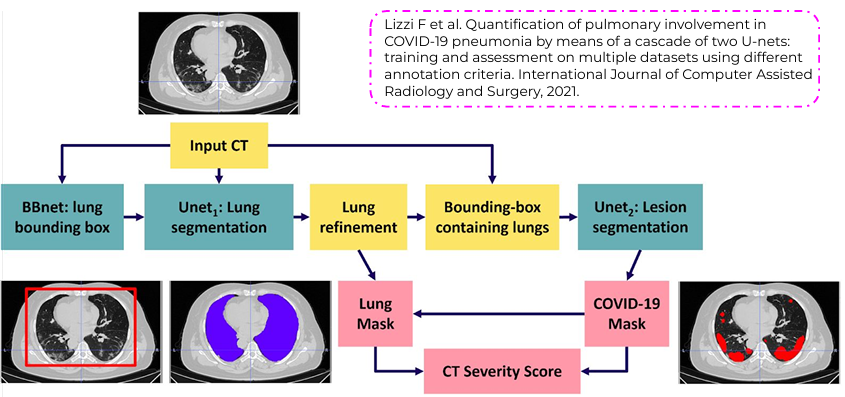
\includegraphics[width=0.85\linewidth]{figuresML_adv/lesson_ml_adv_2_pag_41.png}
\end{center}

The final output of this system provides physicians with crucial metrics, including the total lung volume, the CT Severity Score (CT-SS), and the precise volumes of the different lesion types in both the right and left lungs. 

\textbf{The critical importance of segmentation and explainability}

Working with real-world medical data highlights why aggressive segmentation (like the one performed by U-Net$_1$) is absolutely mandatory. Real datasets are rarely clean or perfect. During the COVID-19 emergency, patients with severe symptoms were often imaged directly in Intensive Care Units (ICUs) using portable, heterogeneous imaging systems. This resulted in extremely noisy images, sometimes with inverted color scales, where patients were poorly positioned and surrounded by external artifacts like breathing tubes, ECG cables, and hospital beds. 

In an initial phase of the study, researchers attempted to train a multi-input CNN to predict patient prognosis (severe vs. not severe) by feeding it raw, unsegmented chest X-Rays combined with clinical features (handling missing clinical data via k-nearest neighbors and mean imputation). The model achieved a seemingly excellent accuracy of around 75\%. 
    
However, when the \textit{Grad-CAM} (Gradient-weighted Class Activation Mapping) explainability algorithm was applied to visualize what the network was actually focusing on, the results were alarming. The network was completely ignoring the lungs. Because the dataset was highly biased by the emergency acquisition settings, the "smart" algorithm had learned to achieve high accuracy by looking at the background artifacts, such as the presence of ICU cables or the specific posture of a bedridden patient rather than analyzing the actual pulmonary pathology. 

This post-hoc explainability analysis perfectly demonstrated that without prior semantic segmentation, a CNN can easily "cheat" by learning confounding variables. By using a U-Net to strictly isolate the lungs and delete the irrelevant background, we force the subsequent classifier to base its predictions solely on genuine anatomical and pathological features.

%\begin{figure}[H]
%    \centering
%    \includegraphics[width=0.85\linewidth]{figuresML/image_5fedfc.png}
%    \caption{U-Net architecture details, dataset aggregation, and resulting case study correlations.}
%\end{figure}

\textbf{Practical implementation and training strategies}

Training these massive fully convolutional networks requires careful data management and specific architectural choices. Because we cannot load the entire dataset into memory, we must use \textbf{data generators}. A data generator dynamically loads small batches of images from the hard drive directly to the GPU during training. 

Furthermore, the generator is responsible for applying \textbf{real-time data augmentation}. By applying random transformations (rotations, zooms, elastic deformations) to the images on the fly, we regularize the network and prevent overfitting. While this approach saves an enormous amount of physical storage space since we do not need to save terabytes of pre-augmented images, it introduces a computational trade-off, as the CPU must spend time processing these transformations during the training loop.

Finally, to train the U-Net for medical segmentation, standard loss functions like MSE are often inadequate. Instead, custom differentiable loss functions must be explicitly programmed. A standard choice is the \textit{dice loss} (often combined with a weighted cross-entropy loss), which directly optimizes the volumetric overlap (volumetric Dice Similarity Coefficient, vDSC) between the predicted segmentation mask and the ground truth.

\subsection{Hands-on example on U-Nets}
To put these concepts into practice, the accompanying exercise involves building a U-Net of our own for lung segmentation. Due to the high memory requirements of processing large medical images, standard in-memory batching is insufficient. 
\begin{itemize}
    \item[-] We will implement a data generator to load batches of data dynamically and apply real-time data augmentation.
    \item[-] We will manually write the decoder path and the residual blocks of the U-Net, and implement the differentiable dice loss mathematically from scratch. 
\end{itemize}
Here is a general scheme of the project.

\begin{center}
    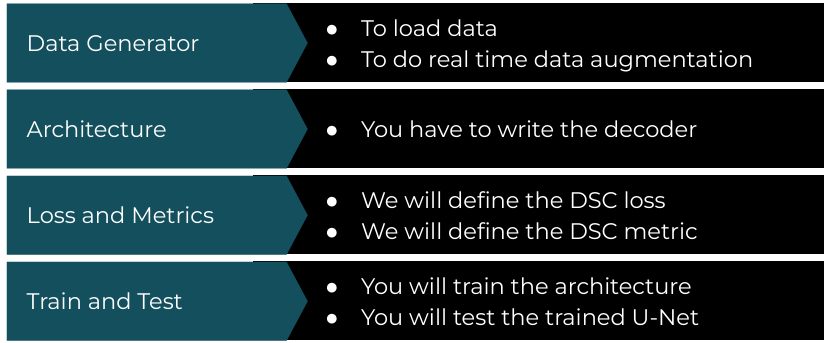
\includegraphics[width=0.6\linewidth]{figuresML_adv/lesson_ml_adv_2_pag_56.png}
\end{center}

Since I have to start a new page in order to input the Notebook in my LaTeX file, here is a photo of McEnroe and Borg taken before the 1980 Wimbledon final to occupy the rest of the page.

\begin{center}
    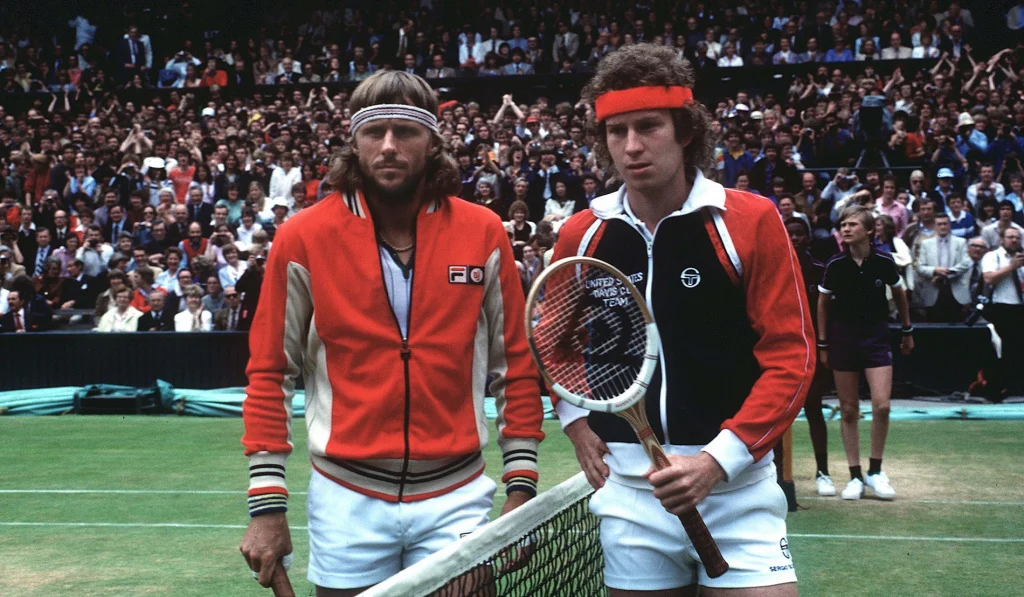
\includegraphics[width=0.4\textwidth]{figuresML_adv/borg_mcenroe_1980.png}
\end{center}

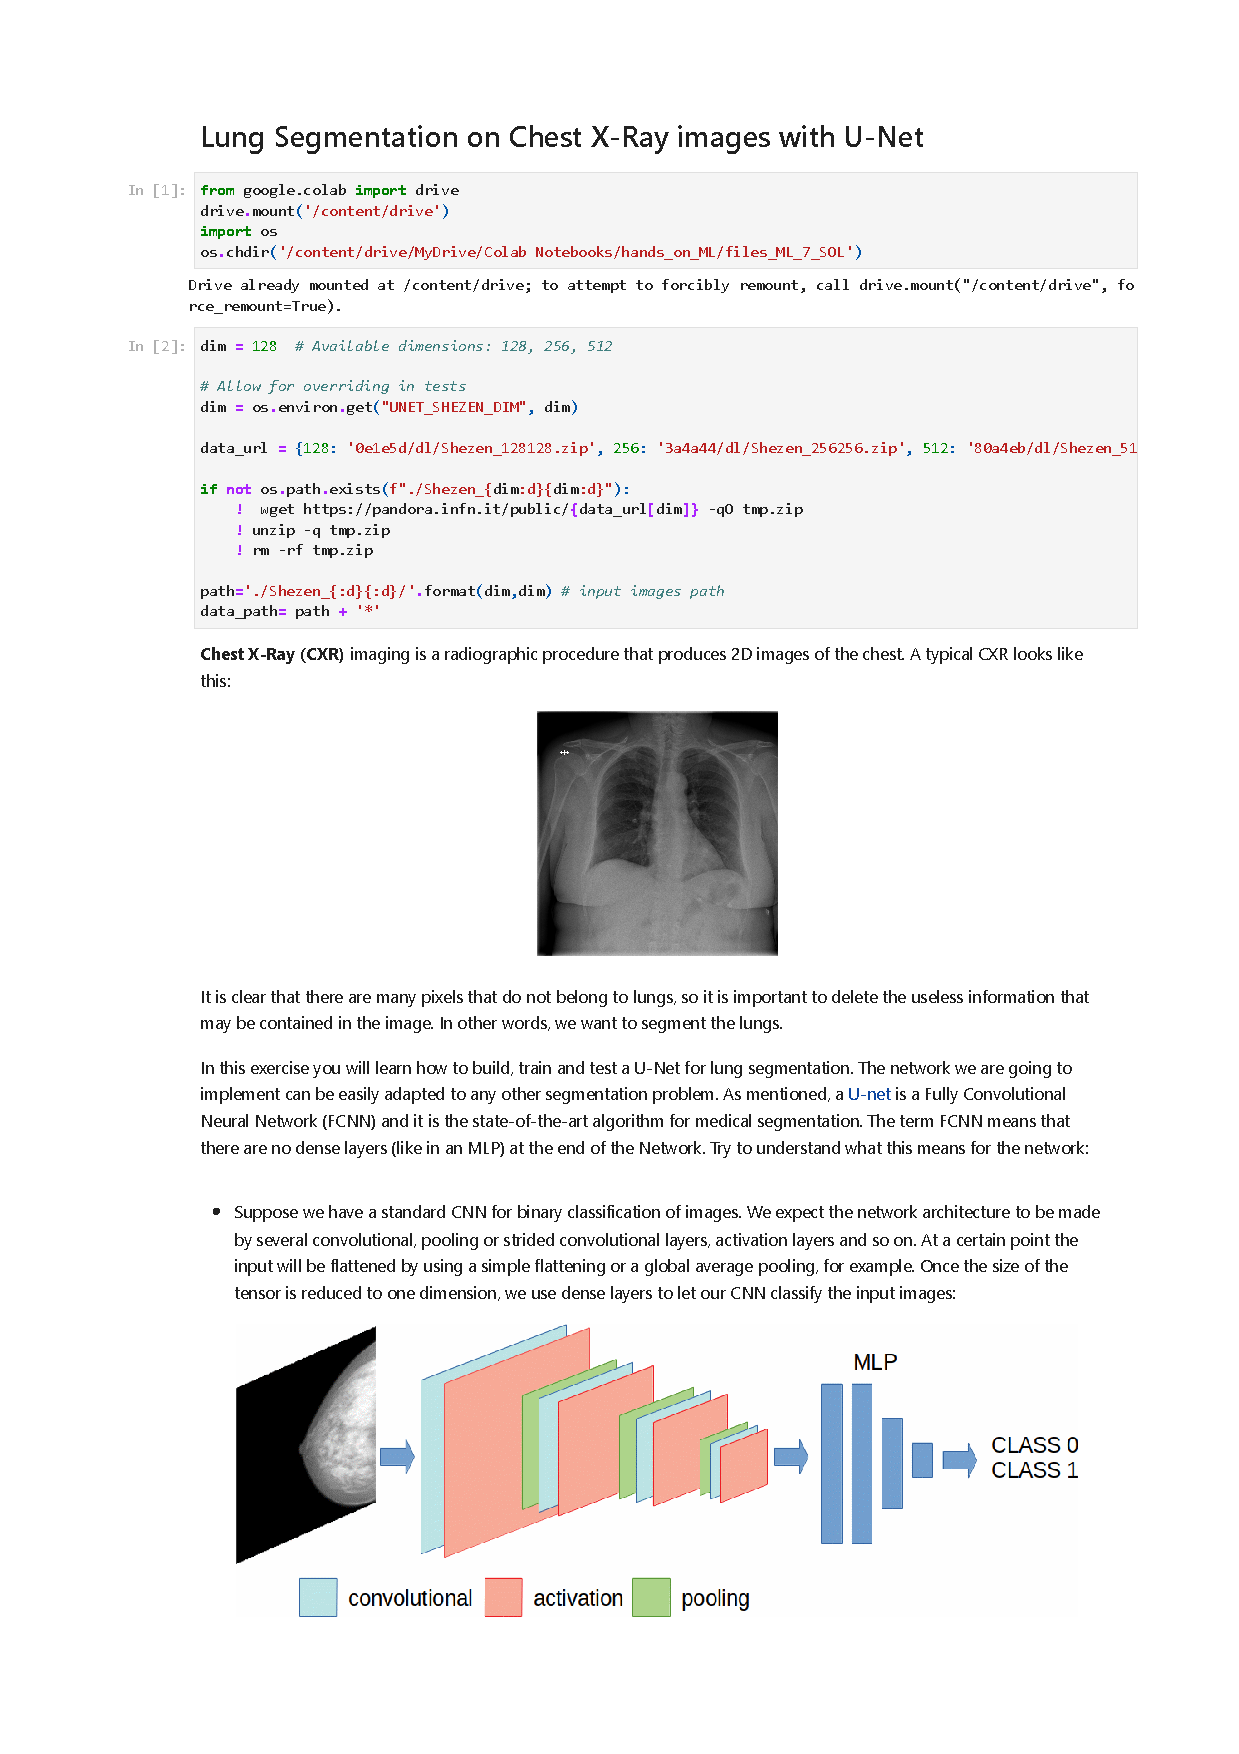
\includepdf[pages=-, pagecommand={\thispagestyle{plain}}]{lezioni/e_ML_adv_2hands_on.pdf} 
% ML_7 nel mio Colab

\begin{comment}
\subsection{Applications in Medical Imaging: LungQuant2.0}
Medical images possess unique challenges compared to standard datasets. They are often extremely high-resolution (e.g., $4000 \times 4000$ pixels) and require the identification of microscopic details. Furthermore, it is not always possible to process them patch-by-patch, making full-image segmentation essential to delete irrelevant anatomical parts from the field of view.

A practical application of U-Nets is the \textbf{LungQuant2.0} system, designed to quantify pulmonary involvement in COVID-19 pneumonia. The pipeline operates as a cascade of networks:
\begin{enumerate}
    \item \textbf{BBNet:} A 3D CNN regression model that predicts the 6 coordinates of the lung's bounding box to standardize the Field of View (FOV).
    \item \textbf{Unet$_1$:} A U-Net that receives the bounded CT scan and performs precise Lung Segmentation, outputting a clear Lung Mask.
    \item \textbf{Unet$_2$:} A subsequent U-Net that operates within the isolated lung mask to segment COVID-19 specific lesions (Ground Glass Opacities and Consolidations).
\end{enumerate}

To train these models, a combined loss function is utilized:
\begin{equation}
    L = \text{Dice}_{loss} + CE_{weighted}
\end{equation}
The loss combines the volumetric Dice Similarity Coefficient (vDSC) with a Weighted Cross-Entropy ($CE_{weighted}$) to heavily penalize errors on small, critical lesion areas. The output allows radiologists to automatically compute metrics like the CT Severity Score and precise lesion volumes.

\subsection{Real life application: U-Net to assess COVID-19 pulmonary damage}
To assess the overall prognosis of a COVID-19 patient, images alone may not be sufficient. We can build a \textbf{Multi-input Convolutional Neural Network} that combines categorical/continuous clinical features (e.g., Age, Temperature, WBC, PaO2, etc.) with Chest X-Ray images. The clinical data is pre-processed (using K-Nearest Neighbors imputation for missing variables and z-scoring), passed through dense layers, and subsequently concatenated with the flattened feature maps extracted from the CNN.

However, when deploying such models on noisy, real-world data (especially datasets acquired during emergency situations like the COVID-19 pandemic), we must verify what the network is actually "looking at". To do this, we use \textbf{Grad-CAM} (Gradient-weighted Class Activation Mapping), a post-hoc explainability algorithm that produces heatmaps highlighting the regions of the image most critical to the network's prediction.

As practically experienced in the lab, if we skip the U-Net lung segmentation step and feed the raw Chest X-Rays directly into the classifier, the network might achieve a deceptively high accuracy (e.g., 75\%). However, applying Grad-CAM reveals a critical flaw: the network is not looking at the lungs at all! Because the dataset is noisy and patients in severe conditions were often imaged in intensive care units with different equipment or poor positioning, the "smart" network learns to classify patient severity by recognizing external background artifacts (like tubes, cables, or image borders) rather than actual pulmonary pathology. \textit{This explicitly demonstrates why aggressive segmentation (via U-Net) to remove non-relevant data is absolutely mandatory in medical imaging.}

\subsection{Practical Exercise: U-Net for Lung Segmentation}
To put these concepts into practice, the accompanying exercise involves building a U-Net for lung segmentation. Due to the high memory requirements of processing large medical images, standard in-memory batching is insufficient. 
\begin{itemize}
    \item \textbf{Data Generators:} You will implement a Data Generator to load batches of data dynamically and apply \textit{real-time data augmentation}. Note that real-time augmentation introduces a trade-off: it saves storage space but heavily increases CPU/GPU computation time during training. 
    \item \textbf{Architecture \& Loss:} You will manually write the decoder path and the residual blocks of the U-Net, and implement the differentiable Dice Loss mathematically from scratch. 
\end{itemize}
\end{comment}
\section{Generative models from differential equations}

We have said thousands of times before that our goal while training a ML algorithm is to minimize a loss function. However, we have never thought about this question in the previous sections: can we trust it? \textbf{Goodhart's law} states that "when a measure becomes a target, it ceases to be a good measure". This means that if we over-optimize an experiment or an algorithm to forcibly obtain a certain measure, we are probably going to get what we want, but that does not mean that such a measure has any significance. We should always remember that our loss function is just a proxy (a good one nonetheless) 
for model performance, not our ultimate goal. Here is a simple analogy:
\begin{itemize}
    \item[-] \textit{Objective}: Increase scientific knowledge.
    \item[-] \textit{Proxy}: Reward scientists for the number of papers.
    \item[-] \textit{Result}: Overproduction of papers and decline in quality of research.
\end{itemize}
Keep this in mind while approaching the next topic.

Notice also that all generative models that we encountered in the last sections have about the same basic structure shown below: starting from a latent space, a NN generates a distribution $\hat{p}(x)$ which is compared with the true data distribution $p(x)$ by the loss function during training.

\begin{center}
    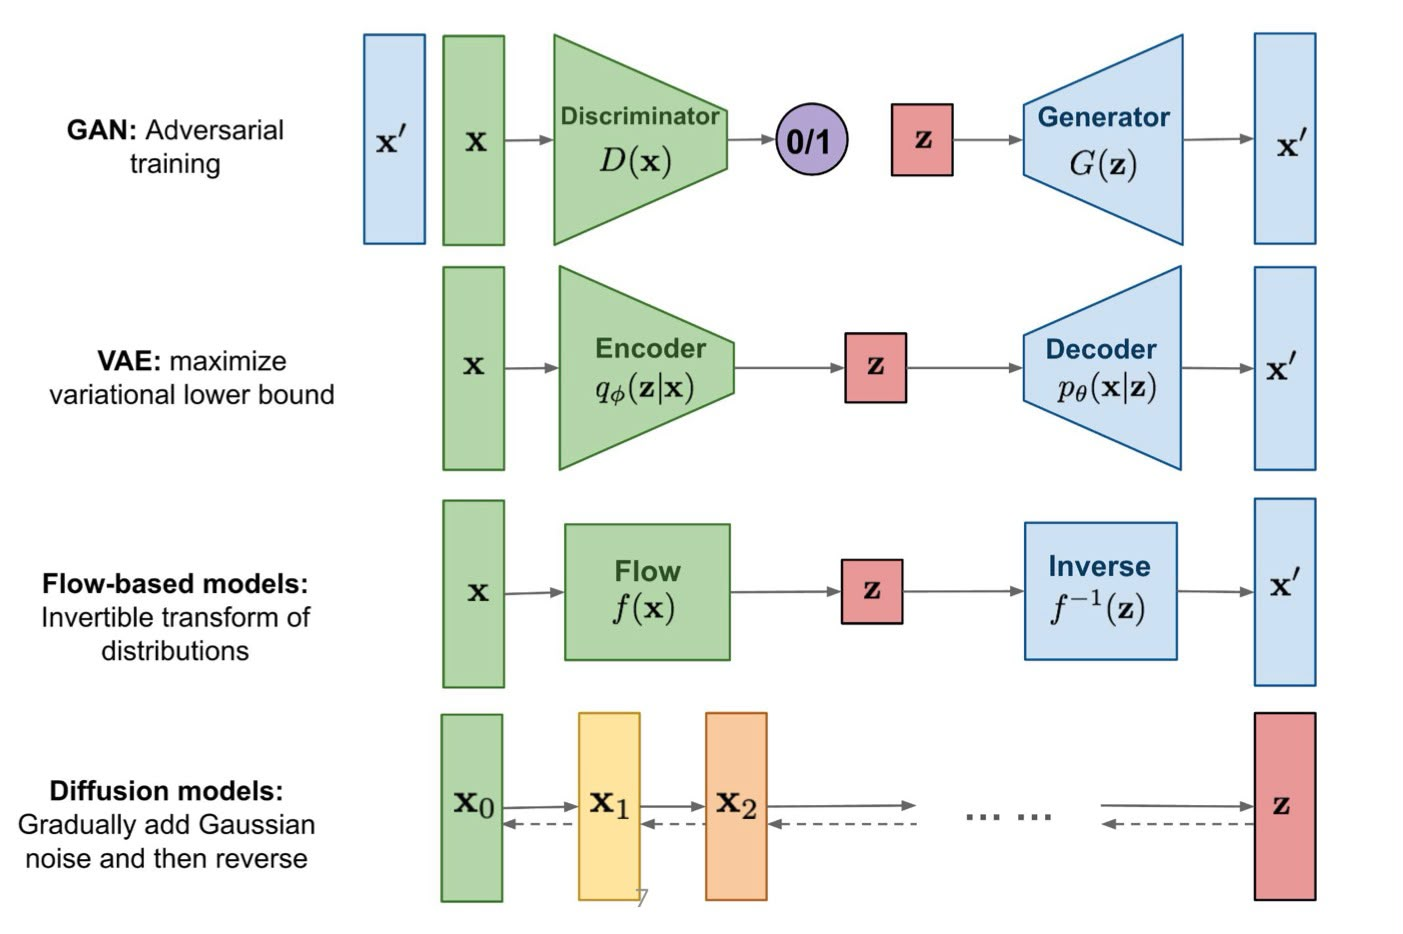
\includegraphics[width=0.49\textwidth]{figuresML_adv/lesson_ml_adv_3_pag_7.png}
    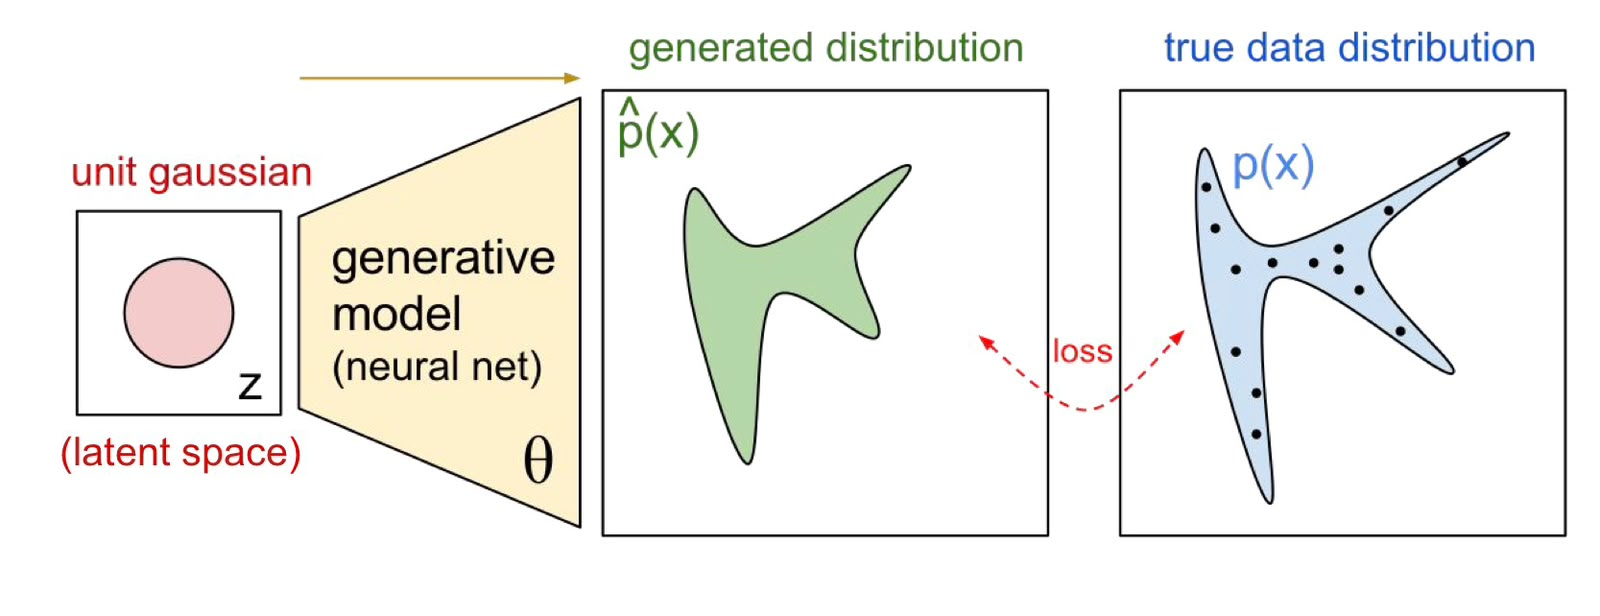
\includegraphics[width=0.49\textwidth]{figuresML_adv/lesson_ml_adv_3_pag_11.png}
\end{center}

Both research and industry are always craving faster, more flexible and expressive generative models and the results are still not perfect, especially in image/video generation (with models like Google Nano Banana and so on). A big improvement was made in 2023, as you can see by comparing these generated images of Will Smith eating spaghetti.

\begin{center}
    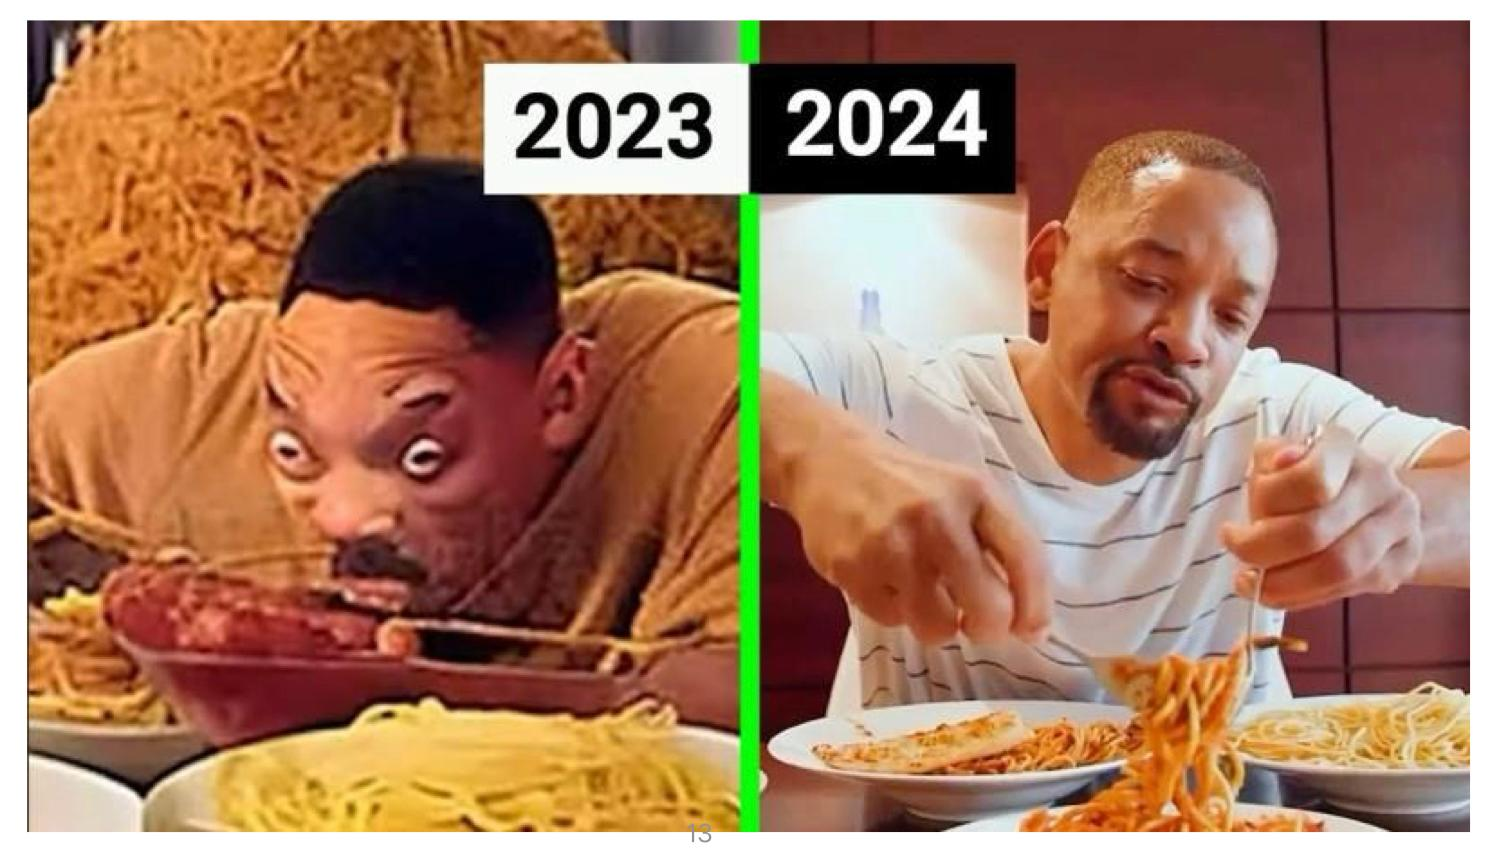
\includegraphics[width=0.55\textwidth]{figuresML_adv/lesson_ml_adv_3_pag_13.png}
\end{center}

What changed between 2023 and 2024? A new paradigm based on differential equations was implemented.

\subsection{From Ordinary Differential Equations to flow models}
Let $P_{init}$ be the distribution of our points in the latent space (e.g. $P_{init} \sim \mathcal{N}(0, I)$). The objective of a generative model is to send $P_{init}$ into a distribution $P_{data}$ in our data space depending on some parameters $\theta$ in our NN. To do so, people realized that Ordinary Differential Equations can be used. Let's go over some basics about them.

A time-dependent \textbf{vector field} is a continuous mapping $u: \mathbb{R}^d \times [0,1] \rightarrow \mathbb{R}^d$ that assigns a tangent vector (representing the instantaneous velocity) to every point $x \in \mathbb{R}^d$ at any given time $t \in [0,1]$. Given such a vector field, a \textbf{trajectory} (or integral curve) is a continuously differentiable curve $x: [0,1] \rightarrow \mathbb{R}^d, \ t \mapsto x_t$ such that its tangent vector at any time $t$ perfectly matches the vector field at that exact position and time. 

Therefore, an \textbf{Ordinary Differential Equation (ODE)}, and in particular its corresponding Cauchy problem, is written as:
\begin{equation}
    \begin{cases}
        \frac{dx_t}{dt} = u_t(x_t) \\
        x_0 = X_0 \quad \text{(initial condition)}
    \end{cases}
\end{equation}

We call \textbf{flow} (or flow map) the function $\psi: \mathbb{R}^d \times [0,1] \rightarrow \mathbb{R}^d$, $(x_0, t) \mapsto \psi_t(x_0)$. The flow describes the simultaneous evolution of the entire state space over time, parameterized by the initial conditions. It can be proven that if $u$ is continuously differentiable (or at least Lipschitz continuous, which guarantees the existence and uniqueness of the solution via the Picard-Lindelöf theorem, as typically assumed in ML algorithms), then $\psi$ is the unique solution of the ODE, satisfying:
\begin{equation}
    \begin{cases}
        \frac{\partial \psi_t(x_0)}{\partial t} = u_t(\psi_t(x_0)) \\
        \psi_0(x_0) = x_0
    \end{cases}
\end{equation}

These are all aspects of the same mathematical object: the vector field $u$ induces the ODE, the individual trajectories $x_t$ solve the ODE for specific starting points, while the flow $\psi$ is a continuous family of such solutions.

\begin{comment}
Let $x: [0,1] \rightarrow \mathbb{R}^d, \ t \rightarrow x_t$ be a trajectory in our data space $\mathbb{R}^d$ and $u: \mathbb{R}^d \times [0,1] \rightarrow \mathbb{R}^d$ a vector field that defines how to "move along" the trajectory. An ODE (in particular its corresponding Cauchy problem) is written as:
\begin{equation*}
    \begin{cases}
        \frac{dx_t}{dt} = u_t(x_t) \\
        x_0 = x_{0} \quad \text{(initial condition)}
    \end{cases}
\end{equation*}

We call \textbf{flow} the function $\psi: \mathbb{R}^d \times [0,1] \rightarrow \mathbb{R}^d$, $(x_0, t) \rightarrow \psi_t(x_0)$ and it can be proven that if $u$ is \textbf{continuously} differentiable % as it should in ML algorithms
then $\psi$ is a solution of the ODE:
\begin{equation*}
    \frac{\partial \psi_t}{\partial t}(x_0) = u_t(\psi_t(x_0))
\end{equation*}
These are all aspects of the same mathematical object: $u$ induces the ODE, the trajectories $x_t$ solve the ODE, while a flow is a family of solutions.
\end{comment}

Now, what does this have to do with ML? Since our goal is to move from a point sampled from $P_{init}$ to one sampled from $P_{data}$, we can identify the first with the initial condition $x_0$ of an ODE, and the latter with a point $x_1$ of the same trajectory. We can then arrive at the definition of a so-called \textbf{flow model}, which is a neural network $u_t^\theta$ that satisfies:
\begin{equation}
    \begin{cases}
        \frac{dx_t}{dt} = u_t^\theta(x_t) \\
        x_0 = X_0
    \end{cases}
\end{equation}
where $\theta$ are the trainable parameters.

\begin{center}
    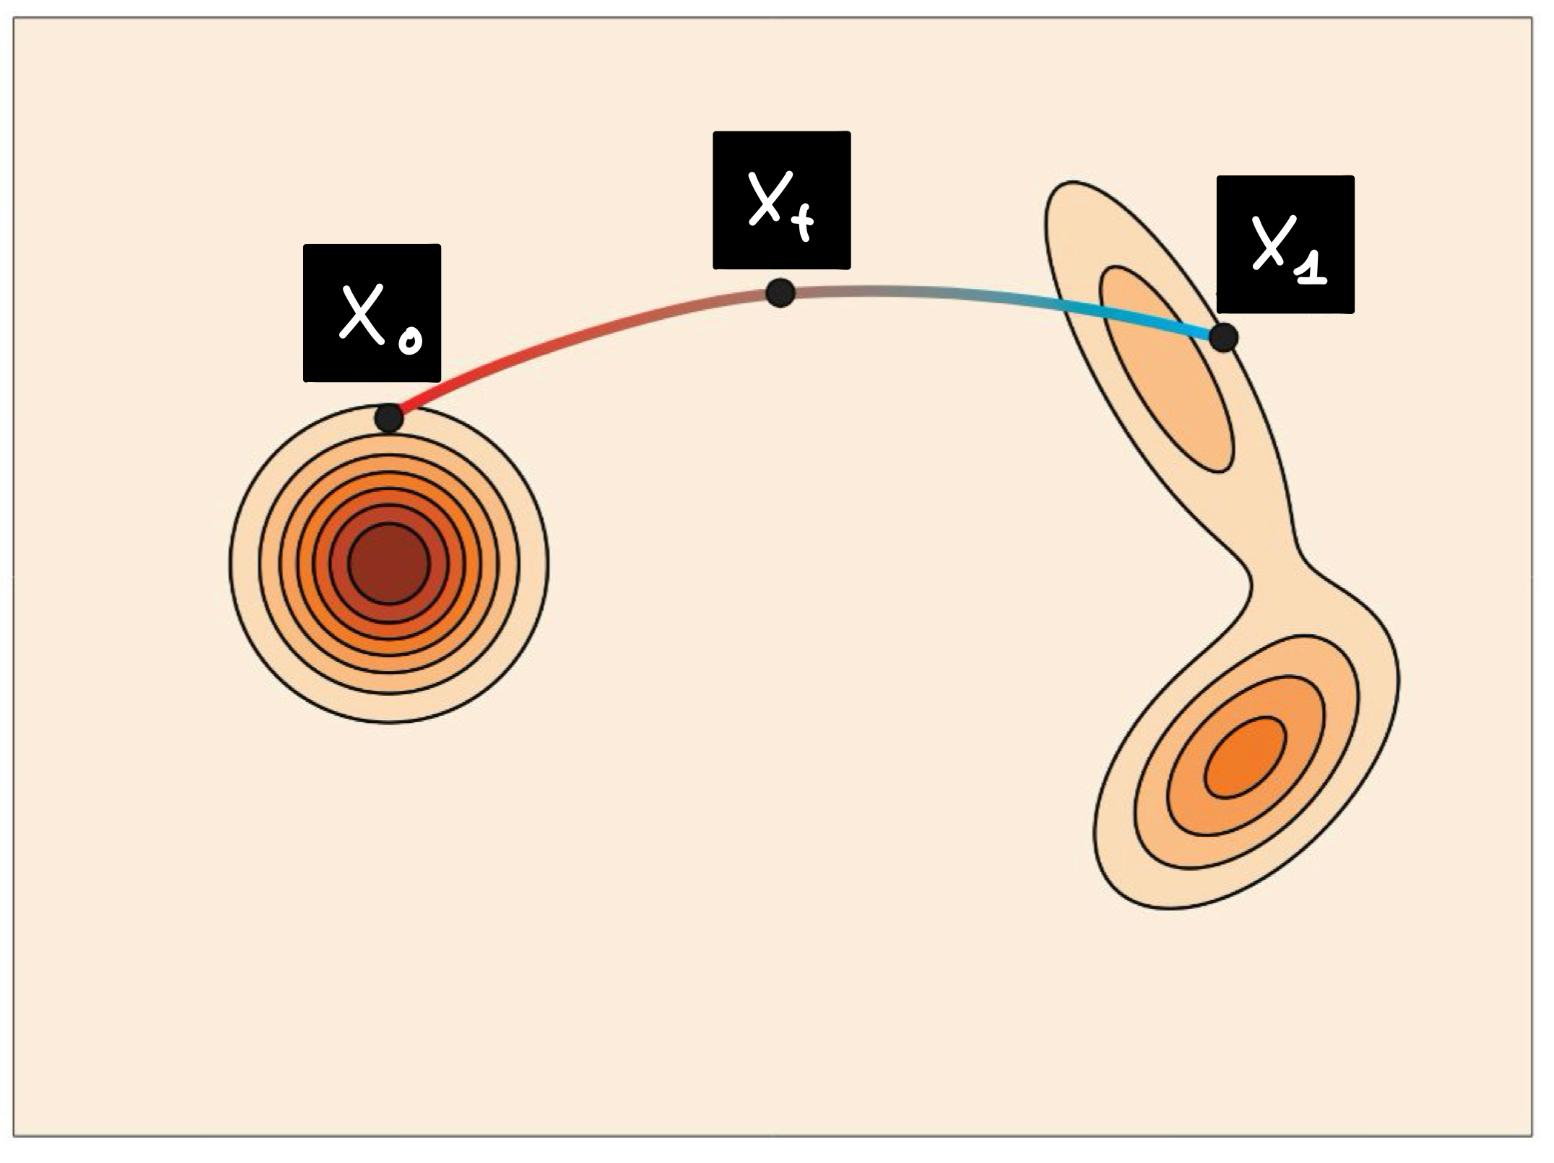
\includegraphics[width=0.45\textwidth]{figuresML_adv/lesson_ml_adv_3_pag_16.png}
\end{center}

Pay attention: even if it is called "flow model", $u_t^\theta$ is actually a vector field  with parameters $\theta$ (by our previous definitions) which takes a data point and the corresponding time and returns a velocity ($\mathbb{R}^d \times [0,1] \rightarrow \mathbb{R}^d$). 

Our main question now becomes clear: how can I create a NN such that the flow that passes through the initial point $\psi_1^\theta(x_0)$ is sampled from $P_{data}$ if computed at $t=1$?

It is fundamental to notice that in this case, \textit{the term "latent space" is just a semantic relic from older models}: in reality the two distributions live in the exact same space and with latent space we can refer to the cloud of starting points. 

For example, if we are working with images $256 \times 256 \times 3$, then our data space would be $\mathbb{R}^{196608}$, just as our latent space. Only a small part of such space is known, i.e. the points corresponding to our training dataset. Given those, we want to train our NN to move from a cloud of normally distributed points ($P_{init} \sim \mathcal{N}(\mu, \sigma)$, which in practice are just images full of random noise, like an old TV with no signal) to the ones corresponding to the images we want to generate ($P_{data}$). 
This movement (schematically represented in the figure below) means solving the "right" ODE defined by the "right" vector field, i.e. our NN.

\begin{center}
    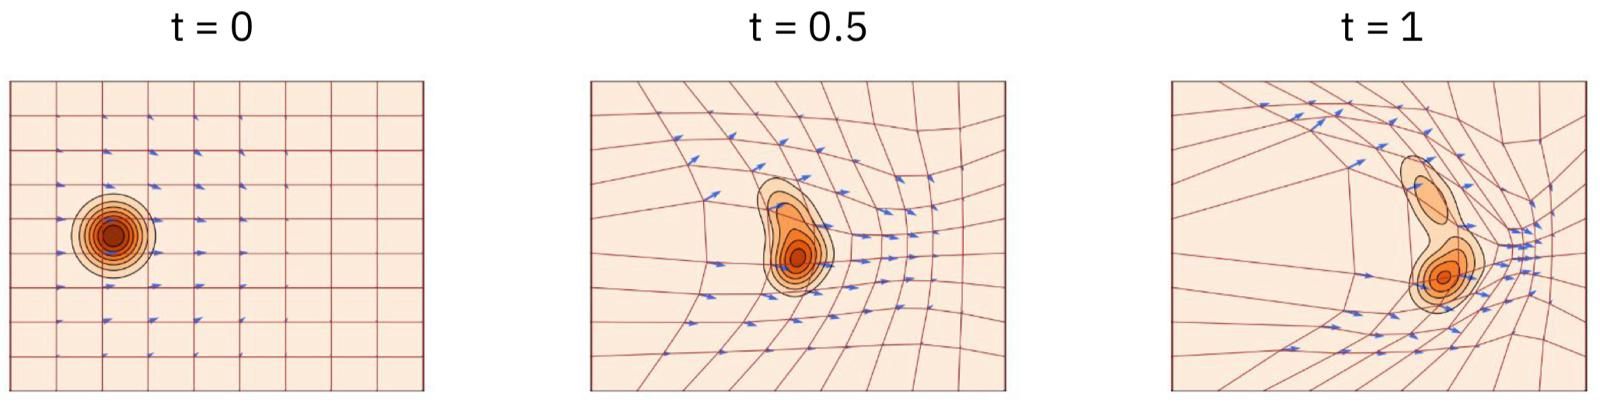
\includegraphics[width=0.8\textwidth]{figuresML_adv/lesson_ml_adv_3_pag_18.png}
\end{center}

\hrulefill

\textbf{Note: From Ordinary Differential Equations to flow models}

While ODEs are used to define flow models, another powerful class of equations called \textbf{Stochastic Differential Equations (SDEs)} forms the mathematical backbone of another ML paradigm: \textbf{diffusion models}. The general form of an It\^o SDE is given by:
\begin{equation}
    dx_t = u_t(x_t) \, dt + \sigma_t \, dW_t
\end{equation}
where $u_t(x_t)$ is called the \textit{drift coefficient} (a deterministic vector field governing the macroscopic movement of the data) and $\sigma_t > 0$ is the \textit{diffusion coefficient}. The term $dW_t$ represents the infinitesimal increment of a standard \textit{Wiener process} (or \textit{Brownian motion}), which continuously injects stochastic noise into the system, effectively causing the state to undergo a random walk. 

Rigorously, a $d$-dimensional standard Wiener process $W_t$ is a continuous-time stochastic process characterized by the following properties:
\begin{enumerate}
    \item $W_0 = 0$ almost surely;
    \item $W_t - W_s \sim \mathcal{N}(0, (t-s)I)$ for $0 \leq s < t$;
    \item The random variable $(W_{t_2} - W_{t_1})$ is independent from $(W_{t_4} - W_{t_3})$ for $0 \leq t_1 < t_2 \leq t_3 < t_4$.
\end{enumerate}
The second condition specifies that the increments of the process are normally distributed with zero mean and a variance that scales linearly with the time step $(t-s)$. The third condition ensures that the increments over non-overlapping intervals are strictly independent.

Because of the injected noise, the solution to an SDE is not a deterministic curve but a \textit{stochastic process}, more precisely a diffusion process or a random-walk. Consequently, every time we solve the equation from the same starting point, the corresponding realization (or sample path) will yield a different, inherently noisy trajectory, as shown in the figure.

\begin{comment}
If ODEs are used to define flow models, there is another class of equations called \textbf{Stochastic Differential Equations (SDEs)} that get us to yet another ML paradigm: \textbf{diffusion models}. The general form of a SDE is the following:
\begin{equation*}
    dx_t = u_t(x_t)dt + \sigma_t dW_t
\end{equation*}
where $\sigma_t > 0$ is called diffusion coefficient while $dW_t$ is the rate of change of a Brownian noise, which essentially injects noise in our solutions causing a random walk. In particular, $W_t$ is an object such that:
\begin{equation*}
    \begin{cases}
        W_0 = 0 \\
        (W_t - W_s) \sim \mathcal{N}(0, (t-s)I) \\
        (W_t - W_s) \ \text{is independent from every other} \ (W_v - W_u) 
    \end{cases}
\end{equation*}
The second condition means that differences between $W$ values at different times of the same process, are distributed as a gaussian distribution with variance that increases with the time interval.

The solution of a SDE is a stochastic process and the corresponding trajectories will change at every iteration as shown in figure.
\end{comment}

\begin{center}
    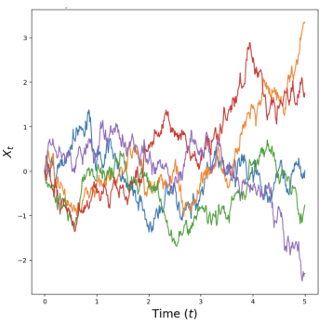
\includegraphics[width=0.3\textwidth]{figuresML_adv/lesson_ml_adv_3_brown.png}
\end{center}

A diffusion model will then be defined by a vector field $u_t^\theta(x_t)$ (the NN) such that
\begin{equation}
    dx_t = u_t^\theta(x_t) \, dt + \sigma_t \, dW_t
\end{equation}
and a diffusion coefficient usually set at a constant value $\sigma_t = \sigma > 0$.

Given the randomness of diffusion models, with such algorithms it is easier to explore the space of solutions. However, experts are slowly realizing that flow models can be just as expressive as their stochastic counterparts.

\hrulefill

\subsection{The long road to flow matching}
Ideally, what we are trying to achieve is just a regression to a target solution $\tilde{u}_t(x_t)$ which would like to be analytically computable from the ODE. This means that our loss function could simply be written as the MSE:
\begin{equation*}
    \mathcal{L}(\theta) = ||u_t^\theta(x_t) - \tilde{u}_t(x_t)||^2
\end{equation*}
Of course, if we knew $\tilde{u}_t(x_t)$ analytically there would be no need to search for $u_t^\theta(x_t)$, so this is certainly not the right reasoning.

In order to find a suitable training target, we need to introduce another object called \textbf{conditional probability path}. Let $y \in \mathbb{R}^d$ be a point in the data space (sampled from $P_{data}$). The conditional probability path of the variable $x \in \mathbb{R}^d$ given $y$ as a function of time ($t \in [0,1]$) is a set $\{P_t(x|y)\}_{t \in [0,1]}$ of probability distributions such that:
\begin{equation*}
    \begin{cases}
        P_0(x|y) = P_{init}(x) \\
        P_1(x|y) = \delta(x-y)
    \end{cases}
\end{equation*}
In other words, as time increases, the distributions of the path "shrink" around the value of $y$, as shown in figure.

\begin{center}
    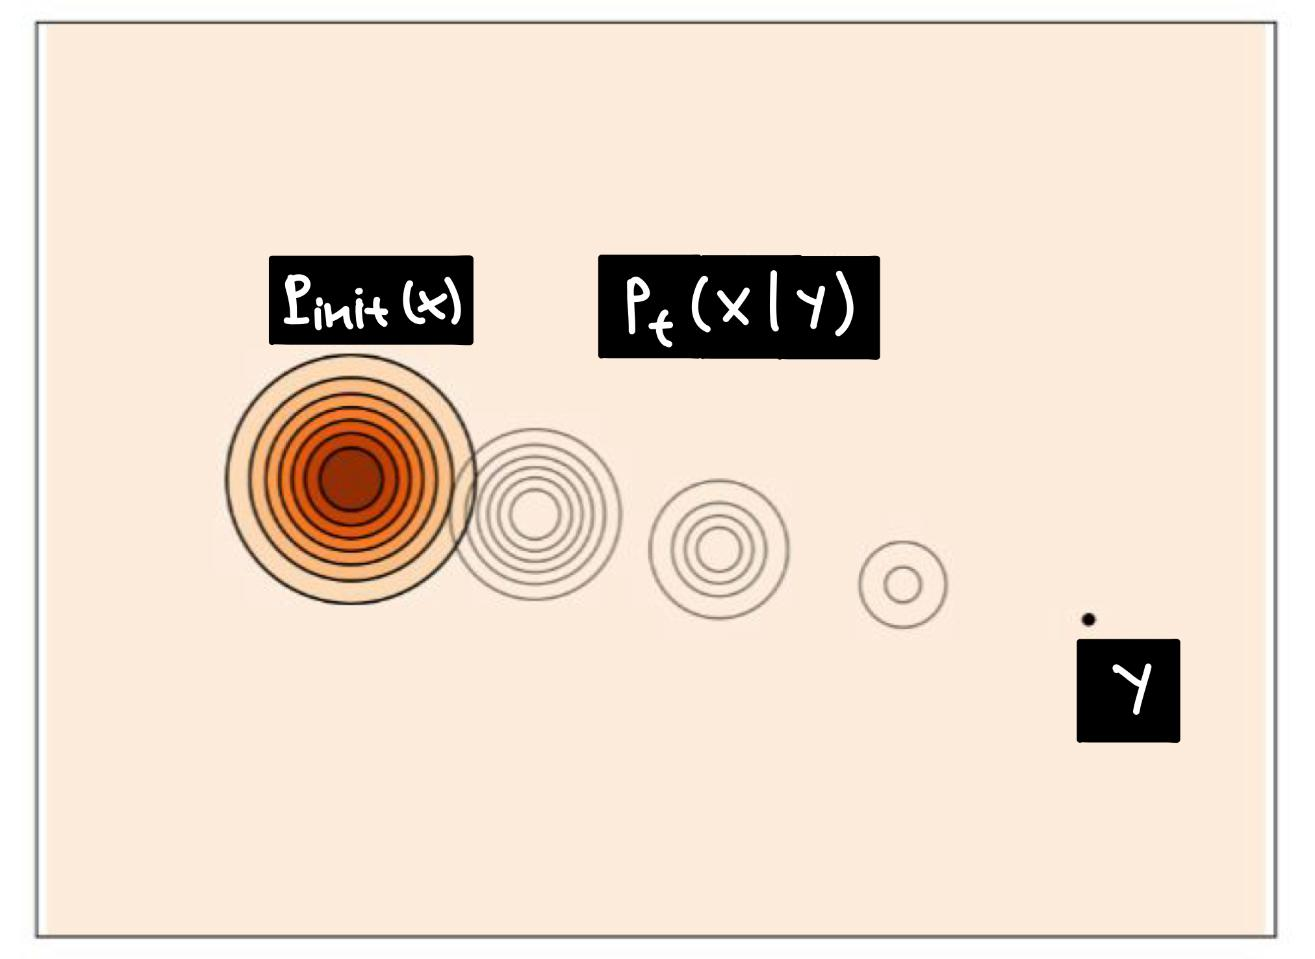
\includegraphics[width=0.45\textwidth]{figuresML_adv/lesson_ml_adv_3_pag_24.png}
\end{center}

A fundamental example is the \textbf{Gaussian conditional probability path}:
\begin{equation}
    P_t(x|y) = \mathcal{N}(\alpha_t y, \beta_t^2 I_d)
\end{equation}
with $\alpha_t, \beta_t$ scalar functions of time. % chosen by us for example
Imposing the 2 conditions above we get:
\begin{equation*}
    \begin{cases}
        P_0(x|y) = \mathcal{N}(\alpha_0 y, \beta_0^2 I_d) = P_{init}(x) = \mathcal{N}(0, I_d) \\
        P_1(x|y) = \mathcal{N}(\alpha_1 y, \beta_1^2 I_d) = \delta(x-y)
    \end{cases}
\end{equation*}
These equations are true if we take $\alpha_t = t$ and $\beta_t = 1-t$, which gives
\begin{equation}
    P_t(x|y) = \mathcal{N}(ty, (1-t)^2 I_d)
\end{equation}
If we then sample $x$ from this probability path we get points distributed in this way:
\begin{equation}
    x_t = \alpha_t y + \beta_t \epsilon = ty + (1-t)\epsilon
\end{equation}
where $\epsilon$ is just random Gaussian noise ($\epsilon \sim \mathcal{N}(0, I_d)$). Of course $x_t \rightarrow y$ for $t \rightarrow 1$, as it should.

Now, notice again what any conditional probability path does: it sends points sampled from the distribution $P_{init}$ into a single point $y$, or similarly $P_{init}$ into $\delta(x-y)$. That is not exactly what we wanted, right? We want the initial points in the latent space to transform into the corresponding generated data points (or analogously $P_{init}$ to "become" $P_{data}$ at $t=1$). 

That can be achieved thanks to the so-called \textbf{marginal probability path} defined as the set $\{P_t(x)\}_{t \in [0,1]}$ such that:
\begin{equation}
    P_t(x) = \int \, dy \ P_t(x|y) P_{data}(y)
\end{equation}
This is an integral over all the possible values of $y$, in other words an \textit{average} over all the possible outcomes of the transformation starting from $x$. That is exactly what we needed, as the marginal probability path is what "moves" $P_{init}$ to $P_{data}$. To better understand this, take a look at what happens at $t=0$ and $t=1$:
\begin{itemize}
    \item[-] At $t=0$: \\ $P_0(x) = \int \,dy \ P_0(x|y) P_{data}(y) = P_{init}(x) \int P_{data}(y) \, dy = P_{init}(x)$
    \item[-] At $t=1$: \\ $P_1(x) = \int \,dy \ P_1(x|y) P_{data}(y) = \int \,dy \ \delta(x-y) P_{data}(y) = P_{data}(x)$
\end{itemize}

That is the perfect tool for our purposes, and the two examples in these next figures should make it even more clear. However, there is an obvious problem: $P_t(x)$ depends on $P_{data}(y)$, which is what we are trying to find, so we cannot actually compute it. 

\begin{center}
    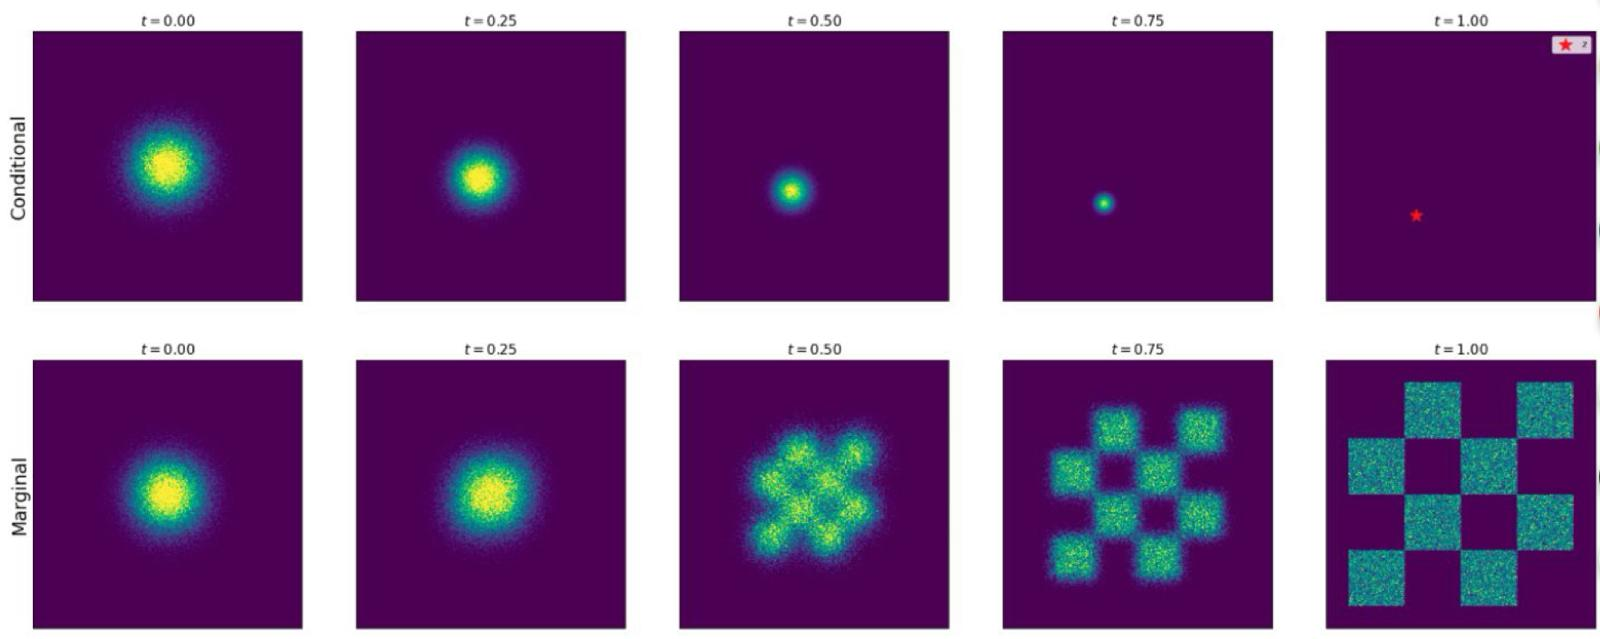
\includegraphics[width=0.9\textwidth]{figuresML_adv/lesson_ml_adv_3_pag_27.png}
    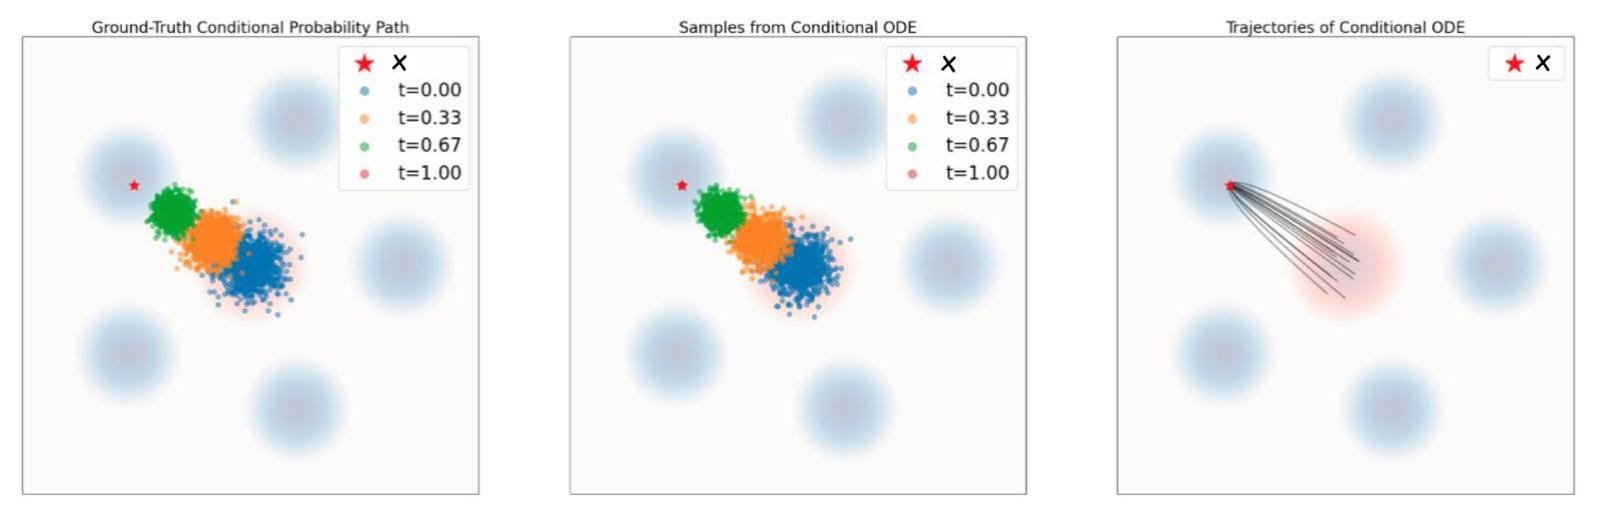
\includegraphics[width=0.9\textwidth]{figuresML_adv/lesson_ml_adv_3_pag_28.png}
\end{center} 

From what we have said up to now, understanding the meaning of these next definitions should come naturally. \\
A \textbf{conditional vector field} is a vector field $u_t^{target}(x|y)$ such that the corresponding ODE follows the conditional probability function, i.e.
\begin{equation}
    \frac{dx_t}{dt} = u_t^{target}(x_t|y) \quad \Rightarrow \quad  x_t \sim P_t(x|y)
\end{equation}
namely if $x_t$ is a solution of the ODE, then it is sampled from $P_t(x|y)$.

Just like before, a pivotal example is that of a \textbf{Gaussian conditional vector field}, which has the following form (you can easily find the explicit computation in the literature):
\begin{equation}
    u_t^{target}(x|y) = \left(\dot{\alpha}_t - \frac{\dot{\beta}_t}{\beta_t}\alpha_t\right)y + \frac{\dot{\beta}_t}{\beta_t}\epsilon
\end{equation}
and with $\alpha_t = t$ and $\beta_t = 1-t$:
\begin{equation}
    u_t^{target}(x|y) = y - \epsilon \quad \text{with } \epsilon \sim \mathcal{N}(0, I_d)
\end{equation}
This means that if we are moving along the conditional probability path from the initial distribution to the data point, the vector field that imposes this transformation is simply the difference between the point sampled from the noise and the data point itself, or, in other words, that we are following a straight path (see figure). In literature these paths are also called \textbf{optimal transfer paths}.

\begin{center}
    \includegraphics[width=0.45\textwidth]{figuresML_adv/lesson_ml_adv_3_pag_25.png}
\end{center}

Following the same logic as before (we want $P_{init}$ to go in $P_{data}$ not in a single point etc\dots) we analogously define the \textbf{marginal vector field} $u_t^{target}(x)$:
\begin{equation}
\begin{aligned}
    u_t^{target}(x) &= \int \,dy \ u_t^{target}(x|y) \frac{P_t(x|y) P_{data}(y)}{P_t(x)} \\
    &= \int \,dy \ u_t^{target}(x|y) P_t(y|x)
\end{aligned}
\end{equation}
where we applied Bayes' Theorem to obtain the second line.
\begin{center}
    \includegraphics[width=0.45\textwidth]{figuresML_adv/lesson_ml_adv_3_pag_26.png}
\end{center}

From this comes a fundamental theorem usually referred to as the \textbf{marginalization trick}: if the conditional vector field $u_t^{target}(x|y)$ induces an ODE from which follows the conditional probability path $P_t(x|y)$, then the marginal vector field $u_t^{target}(x)$ defined by the integral induces in the same way the marginal probability path $P_t(x)$:
\begin{equation*}
    u_t^{target}(x|y) \rightarrow P_t(x|y) \quad \Rightarrow \quad u_t^{target}(x) \rightarrow P_t(x)
\end{equation*}

Again, we are getting closer and closer to a solution, but $u_t^{target}(x)$ still depends on the unknown $P_{data}$ so we are still facing an unsolvable problem in the purely analytical sense. We could attack it numerically, but then our training would become extremely slow, since we would need to solve the $u^{target}(x)$ integral for each training data point. This will all be very useful, but we still need another piece of the puzzle.

Fortunately, one more theorem comes to our aid. Let $x_0$ be our initial point sampled from $P_{init}$ and consider the ODE 
\begin{equation*}
    dx_t = u_t^\theta(x_t) \,dt   
\end{equation*}
where $u_t^\theta$ is our NN and $x_t$ is such that $x_1$ is sampled from $P_{data}$. Let's also define the \textbf{flow matching loss function} $\mathcal{L}_{FM}(\theta)$:
\begin{equation}
    \mathcal{L}_{FM}(\theta) = \mathbb{E}_{t \sim U[0,1], \ x \sim P_t(x)} \left[ ||u_t^\theta(x) - u_t^{target}(x)||^2 \right] \quad \text{\% expected value}
\end{equation}
where $\mathbb{E}$ is the expected value operator. \\
Just like before, if we knew $u^{target}(x)$ there would be no need for $u_t^\theta(x)$. So $\mathcal{L}_{FM}(\theta)$ cannot actually be computed. We can however compute the \textbf{conditional flow matching loss} $\mathcal{L}_{CFM}(\theta)$, defined as:
\begin{equation}
    \mathcal{L}_{CFM}(\theta) = \mathbb{E}_{t \sim U[0,1], \ y \sim P_{data}, \ x \sim P_t(x|y)} \left[ ||u_t^\theta(x) - u_t^{target}(x|y)||^2 \right]
\end{equation}
Even if it is computable, this seems apparently useless for our purposes. However, the following theorem solves all of our doubts: $\mathcal{L}_{CFM}(\theta)$ and $\mathcal{L}_{FM}(\theta)$ are exactly equal up to a \textbf{constant} $C \in \mathbb{R}$ which does not depend on the parameters $\theta$, i.e.
\begin{equation}
    \mathcal{L}_{CFM}(\theta) = \mathcal{L}_{FM}(\theta) + C \quad \text{, } C \in \mathbb{R}
\end{equation}
This means that:
\begin{equation}
    \nabla_\theta \mathcal{L}_{CFM}(\theta) = \nabla_\theta \mathcal{L}_{FM}(\theta)
\end{equation}
so minimizing $\mathcal{L}_{CFM}(\theta)$ automatically minimizes $\mathcal{L}_{FM}(\theta)$, which is what we need.

{ \small
\underline{Proof:} \\
We can expand the squares inside the modules:
\begin{align*}
    \mathcal{L}_{FM}(\theta) &= \mathbb{E} \left[ ||u_t^\theta(x)||^2 - 2u_t^\theta(x)^T u_t^{target}(x) + ||u_t^{target}(x)||^2 \right] \\
    \mathcal{L}_{CFM}(\theta) &= \mathbb{E} \left[ ||u_t^\theta(x)||^2 - 2u_t^\theta(x)^T u_t^{target}(x|y) + ||u_t^{target}(x|y)||^2 \right]
\end{align*}
We have to show that $$\mathbb{E}[u_t^\theta(x)^T u_t^{target}(x)] = \mathbb{E}[u_t^\theta(x)^T u_t^{target}(x|y)]$$ in order to prove that $$\nabla_\theta \mathcal{L}_{FM}(\theta) = \nabla_\theta \mathcal{L}_{CFM}(\theta)$$ In fact, those are the only two terms inside the expected value operator that are different and depend on $\theta$. By definition of expected value we have:
\begin{align*}
    \mathbb{E}[u_t^\theta(x)^T u_t^{target}(x)] &= \int_0^1 \,dt \int \,dx \ P_t(x) u_t^\theta(x)^T u_t^{target}(x) \\
    &= \int_0^1 \,dt \int \,dx \ P_t(x) u_t^\theta(x)^T \left[ \int \,dy \ u_t^{target}(x|y) \frac{P_t(x|y) P_{data}(y)}{P_t(x)} \right] \\
    &= \int_0^1 \,dt \int \,dx \int \,dy \ u_t^\theta(x)^T u_t^{target}(x|y) P_t(x|y) P_{data}(y) \\
    &= \mathbb{E}_{t \sim U[0,1], \ y \sim P_{data}, \ x \sim P_t(x|y)} [u_t^\theta(x)^T u_t^{target}(x|y)]
\end{align*}
which is exactly what we wanted to show. }

Let's get to our final result then, which is the selection of our perfect training target: we can train our network by minimizing a conditional flow matching loss that has the optimal transfer paths $u_t^{target}(x|y) = y - \epsilon$ as its training target:
\begin{equation}
    \mathcal{L}_{CFM}^{OT}(\theta) = \mathbb{E} \left[ ||u_t^\theta(x) - (y - \epsilon)||^2 \right] \quad \text{with } \epsilon \sim \mathcal{N}(0, I_d)
\end{equation}
As you can see, this is an extremely easy loss to write, implement and minimize. In this way the NN learns the ODE transforming the noise to data, as represented below.

\begin{center}
    \includegraphics[width=0.45\textwidth]{figuresML_adv/lesson_ml_adv_3_pag_35.png}
\end{center}

\subsection{Applications of flow matching}
Industrial applications of these new ML paradigms revolve around image and video generation. As a flexible, expressive and powerful form of generative model, these algorithms are suitable for a broad range of tasks, for example:
\begin{itemize}
    \item[-] \underline{Fast simulation of detectors.} The greatest example of this application is what happens at the LHC, where flow models are used to run simulations of particle collisions to prove or disprove some theories. Roughly speaking, LHC will show a read-out that corresponds to the aftermath of a collision, but to reconstruct what caused that readout, you are going to need to create models based on different theories. With the advent of flow models, slow and costly numerical simulations are being substituted by ML algorithms, with a speed-up of 2-3 orders of magnitude.
    \item[-] \underline{Anomaly detection.} Flow models model the PDF of points based on ODEs, which are invertible. In other words, this means that given a new data point $y$, you can reconstruct back the corresponding $x$ in the latent space. If the point deviates from the expected initial distribution (i.e. has a low likelihood) it can be marked as an anomaly. This too is used in LHC to select the events of interest between the $4 \cdot 10^{16}$ collisions per second through trigger systems, which reduce this number to about $\sim 10^5$ events per second.
    \item[-] Many more applications to every task where you need to move from one probability space to another (super resolution, image reconstruction, and thousands of others).
\end{itemize}

As for every generative NN that models the probability density function, the generation can be made conditional (just like it is done with models like ChatGPT and so on).

For a deeper introduction to flow models look at \url{https://diffusion.csail.mit.edu/2025/index.html}.
\section{Recurrent Neural Networks and LSTMs}

As we have extensively discussed in the previous sections, CNNs are exceptionally good at correlating local input information and reducing the network size by sharing weights across repeated patches. However, a question should arise: what if we have multiple objects with absolutely no spatial local correlation, but with multiple features (like the R, G, B channels of a pixel) and we want to process them all in the exact same way? 

\vspace{-4mm}
\begin{figure}[H]
    \begin{minipage}[c]{0.75\textwidth}
        In this specific scenario represented in figure, a $1\times1$ convolution (or simply a Conv1D, since $(x,y)$ coordinates have no physical meaning here) is usually enough. The underlying symmetry we are exploiting is that all the "objects" are fundamentally the same, so we can share the weights along the sequence. 
    \end{minipage}\hfill 
    \begin{minipage}[c]{0.2\textwidth}
        \centering
        \includegraphics[width=0.9\linewidth]{figuresML_adv/lesson_ml_adv_4_pag_2.png}
    \end{minipage}
\end{figure}
\vspace{-7.5mm}

A typical example in experimental physics would be a set of particles in a detector, each carrying information about its 4-momentum vector, tracking hits, calorimeter deposits, and particle identification. We might want to pre-process them one by one identically before feeding them into a higher-level task, but this reasoning quickly hits a wall when dealing with data that do not have a fixed dimension.

\subsection{Recurrent Neural Networks (RNNs)}

To fully exploit time invariance and handle the implied causality of sequences, we must introduce a new architecture: \textbf{Recurrent Neural Networks (RNNs)}. 
But what do we actually mean by \textbf{time invariance} in a sequence? It means that the fundamental properties and the underlying meaning of a pattern do not change based on \textit{when} it occurs. Just like spatial invariance allows a CNN to recognize a specific feature regardless of its position in an image, time invariance ensures that a specific sequence of data carries the exact same meaning whether it appears at the beginning of the measurement (e.g., at $t=1$) or at the end (e.g., at $t=100$). This is exactly why an RNN can share the same weights across all time steps: the function must depend on the pattern's dynamics, not on the clock.

Unlike traditional feed-forward networks, where the information flows strictly in one direction from input to output, RNNs are iterative networks that contain a loop that allows the output of a specific step to be passed again as an input for the subsequent step. This simple but brilliant mechanism allows the network to maintain a "memory" of the previous inputs and build an internal \textbf{state} that represents what the algorithm has "understood" so far in the sequence. \\
Practically, we evaluate the network multiple times. At each time step $t$, the network takes two distinct inputs:
\begin{itemize}
    \item[-] The current element in the sequence, $X_t$.
    \item[-] The output from the previous evaluation, $h_{t-1}$ (the hidden state).
\end{itemize}

To visualize how this actually works, it is extremely useful to look at the RNN not as a single looped unit, but as an \textbf{unrolled} network over the sequence length. If we evaluate an RNN on a sequence of length $N$, we can "unroll" it into $N$ identical connected blocks, as shown in the following figure.

\begin{center}
    \includegraphics[width=0.5\textwidth]{figuresML_adv/lesson_ml_adv_4_pag_5.png} 
\end{center}

Pay attention to a fundamental detail: in the unrolled representation, \textit{all networks "A" are sharing the exact same weights!} We are not creating a massive, deep feed-forward network with independent layers, rather we are applying the exact same function (with the exact same parameters) at each step of the sequence. This is what guarantees the time invariance we discussed earlier: the rule to process the data does not change whether we are reading the first word of a sentence or the hundredth.

\subsection{The vanishing/exploding gradient problem}

While the concept of an RNN is elegant, training it is notoriously difficult. When we train a neural network, we use backpropagation to update the weights based on the gradient of the loss function. For an RNN, we must use a variant called \textbf{Backpropagation Through Time} (BPTT), which essentially means applying the chain rule backward through the entire unrolled network.

This leads to a critical bottleneck known as the \textbf{vanishing or exploding gradient problem}. Since the same weights are used at every step, computing the gradient for the earliest elements in a sequence requires repeatedly multiplying those weights. If the sequence is long, this repeated multiplication causes the gradient to either shrink to zero (vanishing) or grow out of control (exploding), unless the weights are perfectly around the order of 1.

{ \small
\underline{Proof:} \\
Let $\mathcal{E}$ be the total error of the network, and $\theta$ the shared weights. The total gradient is the sum of the gradients evaluated at each individual time step $t$:
\begin{equation}
    \frac{\partial \mathcal{E}}{\partial \theta} = \sum_{1 \le t \le T} \frac{\partial \mathcal{E}_t}{\partial \theta}
\end{equation}
To calculate how the error at time $t$ is affected by the state at a much earlier time $k$ (where $k < t$), we must apply the chain rule across all the intermediate steps. This introduces a product of partial derivatives:
\begin{equation}
    \frac{\partial x_t}{\partial x_k} = \prod_{i=k+1}^t \frac{\partial x_i}{\partial x_{i-1}} 
\end{equation}
Because the state $x_i$ is computed using the recurrent weights $W_{rec}$ and an activation function $\sigma$ (e.g., $x_i = \sigma(W_{rec} x_{i-1} + \dots)$), each term in the product contains $W_{rec}$. Therefore, the chain expansion becomes:
\begin{equation}
    \prod_{i=k+1}^t \frac{\partial x_i}{\partial x_{i-1}} = \prod_{i=k+1}^t W_{rec} \text{diag}(\sigma'(x_{i-1}))
\end{equation}
We are multiplying the same matrix $W_{rec}$ by itself $(t-k)$ times. If the singular values of $W_{rec}$ are strictly less than 1, this product will exponentially decay to 0, resulting in a \textbf{vanishing gradient}. Consequently, the network completely fails to learn long-term dependencies because the earlier inputs receive no gradient updates. Conversely, if the values are strictly greater than 1, the product grows exponentially, leading to an \textbf{exploding gradient} and numerical instability.
}

As a direct result of this mathematical flaw, standard RNNs are highly inefficient to train on long sequences, as they completely lose track of information that appeared too far in the past. To solve this, we must redesign the internal mechanics of the recurrent cell.

\subsection{Controlled flow of information: the birth of LSTMs}

To understand how to fix the structural flaws of standard RNNs, we can first look at how information flows through them compared to CNNs. Take a look at the following figure. As we know, CNNs are strictly focused on local correlations; far regions in an image become correlated only after several pooling layers or in the very last "flatten" step. In contrast, in a standard RNN, at every single step you are forced to process information from the \textit{entire} past. Sometimes, this is simply too much information: a network needs the ability to actively \textit{forget obsolete data} to properly work.

\begin{center}
    \includegraphics[width=0.55\textwidth]{figuresML_adv/lesson_ml_adv_4_pag_6.png}
    \includegraphics[width=0.32\textwidth]{figuresML_adv/lesson_ml_adv_4_pag_6a.png}
\end{center}

We are therefore facing two distinct but related problems:
\begin{enumerate}
    \item The vanishing/exploding gradient, caused by the continuous multiplication of weights across the sequence.
    \item The inability to drop useless past information.
\end{enumerate}

To solve the gradient problem, we must avoid multiplications during backpropagation. The most logical solution is to create a new, separate memory pathway called the \textbf{cell state} ($C_t$), completely distinct from the standard output hidden state ($h_t$). In this architecture the network modifies the cell state primarily via \textit{sums} rather than matrix multiplications, and since the derivative of a sum is simply 1, gradients can flow backward through time without vanishing. \\
However, this solution immediately creates a new issue. If we only \textit{add} information to the cell state at each step, the far past remains exactly as important as the recent past. We have solved the gradient problem, but we have completely destroyed any focus on locality!

To regain control over what is kept and what is discarded, we introduce \textbf{gates}. These are point-wise multiplication operations that use a sigmoid activation function to output a value strictly between 0 and 1. They act as trainable valves: if a gate outputs 0, the information is completely blocked (resetting the state); if it outputs 1, the information is left unchanged. These gates can be applied directly to the cell state (to forget past info) or to the input/output of the network.

The \textbf{Long Short-Term Memory (LSTM)} network is the very first architecture that successfully introduced and combined all these ideas.

\begin{center}
    \includegraphics[width=0.75\textwidth]{figuresML_adv/lesson_ml_adv_4_pag_8.png}
\end{center}

Looking at the anatomy of an LSTM cell in the figure above, we can easily identify the mathematical implementation of our logical steps:
\begin{itemize}
    \item[-] \textbf{Forget gate ($F_t$)}: A sigmoid layer that looks at $H_{t-1}$ and $X_t$, outputting a number between 0 and 1 for each number in the cell state $C_{t-1}$. This is the network deciding what to forget.
    \item[-] \textbf{Input gate ($I_t$)} and \textbf{Candidate memory ($\tilde{C}_t$)}: Another sigmoid gate ($I_t$) decides which values we will update. Simultaneously, a $\tanh$ layer creates a vector of new candidate values ($\tilde{C}_t$) that could be added to the state.
    \item[-] \textbf{Cell State Update}: The old state $C_{t-1}$ is multiplied by $F_t$ (forgetting what we decided to drop), and then we \textit{add} $I_t * \tilde{C}_t$ (the new candidate information). This is the linear, additive path that saves our gradients!
    \item[-] \textbf{Output gate ($O_t$)}: A final sigmoid gate decides what parts of the cell state will be outputted as the new hidden state $H_t$.
\end{itemize}

Notice the rigorous choice of activation functions: sigmoids ($\sigma$) are exclusively used for the gates because we need a $0/1$ behavior, while $\tanh$ is used for the actual information to keep the internal values stabilized and bounded within a limited range.

The ultimate advantage of these gated units is their contextual adaptability. For example, when processing a text sequence, the network might learn that encountering a "space" character means the current word is over. The forget gate can use this specific trigger to reset the state, throwing away the character-level memory of the previous word and starting fresh to accumulate information for the next one.

\hrulefill

\textbf{Note: Gated Recurrent Units (GRU)}

A popular and computationally lighter alternative to the LSTM is the \textbf{Gated Recurrent Unit (GRU)}.  As you can see in the diagram below, the GRU simplifies the architecture by merging the cell state and the hidden state into a single pathway. Consequently, this also merges the input and forget gates into a single update mechanism. 

\begin{center}
    \includegraphics[width=0.4\textwidth]{figuresML_adv/lesson_ml_adv_4_pag_9.png}
\end{center}

Because of this architectural simplification, the output information is only summed, meaning there is no longer a separate, privileged path exclusively dedicated to preserving previous time step information. However, it is important to note that since all states and gates are vectors, the network still retains the ability to optimize when to forget on different timescales for different elements of those vectors.

\hrulefill

\subsection{Processing time series and architectural configurations}

One of the greatest strengths of Recurrent Neural Networks and LSTMs is their extreme architectural flexibility. Unlike standard CNNs or MLPs that require a fixed input and output size, recurrent networks can be easily adapted to process variable numbers of inputs and outputs. 

Depending on the specific task, we can arrange the unrolled network into different configurations (some represented below):
\begin{itemize}
    \item[-] \textbf{One-to-One}: This is essentially the standard feed-forward behavior, processing a single input to produce a single output.
    \item[-] \textbf{One-to-Many}: A single input is used to generate a sequence of outputs (e.g. image captioning, where one image generates a sentence of words).
    \item[-] \textbf{Many-to-One}: A sequence of inputs is processed to produce a single output. In this configuration, we typically ignore the intermediate outputs and \textit{just take the final cell state} to make our prediction (e.g. sentiment analysis of a text).
    \item[-] \textbf{Many-to-Many (Synchronous)}: We get exactly one output for each input step. The network produces a sequence of the exact same length as the input sequence (e.g. classifying every single frame of a video in real-time).
    \item[-] \textbf{Many-to-Many (Asynchronous)}: The input sequence and the output sequence have different, variable lengths. This is arguably the most useful architecture for complex tasks like text translation, and it requires a specific setup known as the Encoder-Decoder architecture.
\end{itemize} 

\begin{center}
    \includegraphics[width=0.3\textwidth]{figuresML_adv/lesson_ml_adv_4_pag_11.png}
    \includegraphics[width=0.35\textwidth]{figuresML_adv/lesson_ml_adv_4_pag_11a.png}
\end{center}

When we need to map an input sequence to an output sequence of a different length, we cannot rely on a simple synchronous mapping. Instead, we use our well known \textit{encoder-decoder} (or \textit{Sequence2Sequence}) architecture, which is realized by combining two separate RNNs as shown in the figure below.

\begin{center}
    \includegraphics[width=0.5\textwidth]{figuresML_adv/lesson_ml_adv_4_pag_11b.png}
\end{center}

We have seen before how the logic behind this can be beautifully simple yet extremely powerful:
\begin{enumerate}
    \item \textit{The encoder}: The first RNN processes the input sequence step by step. Its sole purpose is to compress all the variable-length information of the sequence into a fixed-dimension latent space. Once the input sequence is over, the final \textit{cell state} of this encoder contains the "meaning" of the entire sequence.
    \item \textit{The decoder}: The second RNN takes over to generate the new sequence. Crucially, the final cell state of the encoder is explicitly passed as the \textit{initial state} for the decoder. The decoder then decompresses this state step by step to build the output.
\end{enumerate}

Since the output sequence has a variable length, the decoder needs to know when to stop generating new elements. To solve this, we must define a specific \textit{STOP token} (such as \texttt{<EOL>}, End-Of-Line). The decoder will continue to generate outputs iteratively until it predicts this exact token, at which point the generation halts.

\subsection{Data formatting and sequence management}

Before feeding data into an LSTM, the input sequence is often pre-processed element by element. In modern Deep Learning, this is typically done through an embedding layer, which maps discrete variables (like words or categorical features) into dense, continuous vectors of a fixed dimension.

Consequently, the data tensor passed to the recurrent layers usually possesses three dimensions:
\begin{itemize}
    \item[-] $N$: The batch size, i.e. number of independent sequences processed simultaneously.
    \item[-] $L$: The sequence length: while sequences can theoretically have variable lengths, in practice, to perform parallel tensor calculus on a GPU, we must define a fixed maximum length.
    \item[-] $F$: The number of features per element, or the dimension of the embedding space.
\end{itemize}

Since we force sequences into a fixed maximum length $L$, shorter sequences must be \textbf{padded} (usually with zeros) to fit the tensor. However, padding introduces a subtle but dangerous problem: if the network processes a long string of zeros at the end of a sequence, it might "learn from padding" or dilute the valuable information stored in its cell state before reaching the final output.

To prevent this, several theoretical and practical countermeasures can be implemented:
\begin{itemize}
    \item[-] \textit{Masking layers}: These explicitly tell the network to ignore padded values, skipping the computation for those specific steps.
    \item[-] \textit{Reversing the sequence order}: By feeding the sequence backward, the padding occurs at the beginning. This ensures that the actual meaningful data is processed last, meaning the "freshest" memory in the final cell state corresponds to the most important information.
    \item[-] \textbf{Bidirectional RNNs}: Instead of processing the sequence only left-to-right, a Bidirectional RNN processes it simultaneously in both directions using two separate hidden states. This ensures that the network has both past and future context at every single step of the sequence, making it incredibly robust.
\end{itemize}

\subsection{Practical implementation in PyTorch and Keras}

Now that we have established the theoretical foundations of sequence processing, let's take a look at how we can actually code these architectures. First, some general notions on how PyTorch and Keras handle LSTM layers and sequence management that can be useful for your software.

When defining an LSTM in PyTorch, you must pay close attention to the expected input shape. By default, PyTorch uses a "batch second convention", meaning it expects tensors formatted as \texttt{(Sequence, Batch, Features)}. While this is implemented as a memory optimization under the hood, it is generally counterintuitive and not strictly relevant for standard toy examples or simpler problems. Therefore, it is highly suggested to use the \texttt{batch\_first=True} option, which restores the more standard \texttt{(Batch, Sequence, Features)} shape for an easier understanding of the code.

Here is a typical initialization:

\begin{verbatim}
import torch.nn as nn

lstm = nn.LSTM(input_size=10, hidden_size=20, batch_first=True)
output, (h_n, c_n) = lstm(input_batch)
\end{verbatim}

As you can see, evaluating the LSTM layer explicitly returns three distinct objects:
\begin{enumerate}
    \item \texttt{output}: The hidden features for each time step in the sequence. Its shape will be \texttt{(Batch, Seq, Hidden)}.
    \item \texttt{h\_n}: The hidden state of the very last step. Its shape will be \texttt{(Num Layers, Batch, Hidden)}.
    \item \texttt{c\_n}: The cell state of the very last step.
\end{enumerate}

Furthermore, to avoid performing pointless calculations on padded zero-values (as we discussed in the previous section), PyTorch implements an elegant optimization using the \texttt{PackedSequence} class. This method removes the zeros while keeping track of the original indices, computes the math through the LSTM, and finally places the zeros back in their correct positions:

\begin{verbatim}
packed_input = pack_padded_sequence(input, lengths)
# LSTM evaluation returning packed_output
output = pad_packed_sequence(packed_output)
\end{verbatim}

The logic is incredibly similar in Keras. An LSTM layer can be configured to return just the output of the last iteration, the whole sequence of outputs, the gated output of the memory (the hidden state), and the cell state. 

We can control this behavior using the \texttt{return\_sequences} and \texttt{return\_state} boolean parameters:

\begin{verbatim}
from keras.models import Model
from keras.layers import Input, LSTM
from numpy import array

inputs1 = Input(shape=(5, 1))
lstm1, state_h, state_c = LSTM(1, return_state=True, return_sequences=True)(inputs1)
model = Model(inputs=inputs1, outputs=[lstm1, state_h, state_c])

data = array([0.1, 0.2, 0.3, 0.4, 0.5]).reshape((1, 5, 1))
print(model.predict(data))

[Output]
1/1 [==============================] - 0s 145ms/step
[array([[[0.01334215],
         [0.03582103],
         [0.06321989],
         [0.09452317],
         [0.12837262]]], dtype=float32), 
 array([[0.12837262]], dtype=float32), 
 array([[0.2541938 ]], dtype=float32)]
\end{verbatim}

If you run this code, the output will contain three distinct arrays: the full sequence of 5 hidden states, the final hidden state (\texttt{state\_h}), and the final cell state (\texttt{state\_c}). You will immediately notice that the specific value of \texttt{state\_h} perfectly matches the exact last element of the \texttt{lstm1} sequence array, mathematically confirming that the network is outputting the final time-step representation alongside the full sequence history.

\section{Hands-on examples for LSTMs}

To put these concepts into practice, the accompanying exercises involve building LSTM architectures for two different sequence tasks.

\begin{itemize}
    \item[-] \textit{LSTM Encoder Exercise}: We try building from scratch an LSTM that, given a sequence of two-dimensional vectors, finds the maximum norm and the position in the sequence. We will need to generate some data and build a network with one LSTM layer followed by a Dense one. Here is the link to the Notebook: \url{https://colab.research.google.com/drive/1m9Ybt08aNbNNJgVCVEWa03bnfaNqaNJh?usp=sharing}.
    \item[-] \textit{LSTM Decoder exercise}: We will teach multiplication tables to our LSTM. We give the network a base $B$ and a number $N$ of values we want, and it should produce a sequence $[1*B, 2*B, \dots, N*B]$. Let's try to use an "end of sequence" token (e.g., -1). Here is the link to the Notebook: \url{https://colab.research.google.com/drive/10waGCBQG_iDC2ewYZKGjUBR3YQ50BnO7?usp=sharing}
\end{itemize}

Since I have to start a new page in order to input the Notebook in my LaTeX file, here is a compilation of photos from the Grand Slam Tournaments of 1989. In order:
\begin{itemize}
    \item[-] Ivan Lendl with the 1989 Australian Open trophy (\textit{upper left});
    \item[-] Michael Chang after winning the 1989 Roland Garros against Stefan Edberg (after eliminating Ivan Lendl in the quarterfinals in a legendary match of psychological warfare, \textit{upper right});
    \item[-] Boris Becker after winning the 1989 Wimbledon final against Stefan Edberg (\textit{bottom left});
    \item[-] Steffi Graf and Boris Becker after winning the 1989 Men's and Women's singles at the US Open for Germany (\textit{bottom right}).
\end{itemize}

\begin{center}
    \includegraphics[width=0.23\textwidth]{figuresML_adv/ivan_lendl_1989.png}
    \includegraphics[width=0.5\textwidth]{figuresML_adv/michael_chang_1989.png}
\end{center}
\begin{center}
    \includegraphics[width=0.25\textwidth]{figuresML_adv/boris_becker_1989.png}
    \includegraphics[width=0.5\textwidth]{figuresML_adv/becker_graff_1989.png}
\end{center}


%\includepdf[pages=-, pagecommand={\thispagestyle{plain}}]{lezioni/e_ML_adv_4ahands_on.pdf}
%ML_8a nel mio colab

%\includepdf[pages=-, pagecommand={\thispagestyle{plain}}]{lezioni/e_ML_adv_4bhands_on.pdf}
%ML_8b nel mio colab
\section{Introduction to transformers}\label{sec:transformers}

One of the most important innovations in the modern Machine Learning world is undoubtedly the advent of Transformers. Architectures like ChatGPT, Gemini, and a myriad of other AIs are completely revolutionizing the technological landscape. In fact, if you ask experts, this architecture has changed the field of machine learning just as profoundly as the invention of the transistor changed microelectronics! 

\subsection{The Attention Mechanism}

The core idea behind Transformers is relatively simple and originates from Natural Language Processing (NLP). Imagine a simple task: we want to guess the missing word in the middle of a sentence using an ML algorithm. As we previously discussed, a sentence is essentially a sequence of words, making it natural to think that this problem could be solved by a Recurrent Neural Network (RNN). However, we also know the severe limitations of those algorithms, with the vanishing or exploding gradient problem being the primary bottleneck.

An idea that could be far more efficient is to stop processing words sequentially. Instead, we can place them in a matrix, where both the rows and the columns correspond to the words in the sentence. Each entry in this matrix is a number (from 0 to 1) representing the correlation or importance between two words. Superfluous information gets an entry of 0, while highly relevant connections get an entry closer to 1. 

Given the natural mathematical equivalence between matrices and graphs, we can view this sentence as a fully connected graph. Every word is a node, and every connection (matrix entry) is an edge assigned a specific weight $\alpha \in [0,1]$. 

Let us formulate this from a message passing point of view. In a generic GNN, the message passing is basically an update function. The pooling operation aggregates messages "democratically". We update a node's hidden representation $h_i$ by simply summing the messages from its neighbors $j$ \footnote{This is a simplified version of Eq. \ref{eq:node_update}.}:
\begin{equation}
    h_i' = \phi^v\left(h_i, \sum_j \phi^e(h_i, h_j)\right)
\end{equation}
However, it is intuitive to say that certain messages might be vastly more important than others. We want to generalize this to an \textbf{attentional message passing} by weighting the incoming messages with our factor $w_{ij}$:
\begin{equation}
    h_i' = \phi^v\left(h_i, \sum_j w_{ij}(h_i, h_j) \phi^e(h_j)\right)
\end{equation}
During the message passing step, the pooling operation (the sum in this case) ensures that the most relevant messages (those coming from edges with higher weights) contribute the most to the node's update. This is the so-called \textbf{attention mechanism}, briefly introduced in Sec. \ref{sec:intro_att_mech}.

\subsection{The Key, the Query, and the Value}

We immediately realize that we now allow for a weighting mechanism of the importance of the information to be passed to the receiver node $i$. The overall attention algorithm is based on the definition of these weights $w_{ij}$. But how do we actually find them? We certainly do not know them a priori, so they must be learnable parameters that the neural network automatically optimizes during training via gradient descent. To do this, we introduce three distinct concepts: the \textbf{Key}, the \textbf{Query}, and the \textbf{Value}.

This mechanism inherits its logic directly from how large databases operate. Imagine you are on YouTube and you want to search for videos about cats. You type "cat" into the search bar: your search term is the \textit{query} (the anchor). Meanwhile, all the videos in the database are indexed by a \textit{key} (their metadata or tags). The database computes the similarity between your query and the keys to return the most relevant videos.

In the context of our graph, we translate this process into trainable neural networks:
\begin{itemize}
    \item[-] \textbf{The Query ($\vec{q}_i$)}: This is an encoded message of the \textbf{receiver} node $i$ (the anchor looking for information). It is defined via a neural network $\phi^q$ as $\phi^q(h_i) = \vec{q}_i$.
    \item[-] \textbf{The Key ($\vec{k}_j$)}: This is an encoded message of the \textbf{sender} node $j$ (the database entry). It is defined via a neural network $\phi^k$ as $\phi^k(h_j) = \vec{k}_j$.
\end{itemize}

To find the importance of the message from node $j$ to node $i$, we compute the scalar product between the query and the key:
\begin{equation}
    w_{ij} = \vec{k}_j \cdot \vec{q}_i
\end{equation}
This dot product expresses the similarity between the two vectors in the hidden space. During training, the query and key networks will change their weights until the representations of important messages become similar (meaning their scalar product will be large). 

However, this scalar product can theoretically output any real number from $-\infty$ to $+\infty$. If node $i$ receives messages from multiple neighbors, we intuitively want these weights to act as probabilities, meaning they must be bounded between 0 and 1, and their total sum must equal  1. 
We already mentioned another ML context where we take raw real numbers ranging from $-\infty$ to $+\infty$ and normalize them so they sum to 1: multi-class classification! Just like we do to extract class probabilities, we apply a \textit{softmax} function over all the sending nodes $j \in \mathcal{N}_i$:
\begin{equation}
    \alpha_{ij} = \text{softmax}_j(\vec{k}_j \cdot \vec{q}_i) = \frac{\exp(\vec{k}_j \cdot \vec{q}_i)}{\sum_{l \in \mathcal{N}_i} \exp(\vec{k}_l \cdot \vec{q}_i)}
\end{equation}

Once we have computed this normalized weight, we need the actual information to transmit. We do not just send the raw hidden state; instead, we encode it into a new representation.
\begin{itemize}
    \item[-] \textbf{The Value ($\vec{v}_j$)}: This is the actual message that is sent by node $j$, which will be weighted by $\alpha_{ij}$. It is defined via a neural network $\phi^V$ as $\phi^V(h_j) = \vec{v}_j$. 
\end{itemize}

It becomes clear why this is called the "value" of the message: it is the core information encoded to be transmitted, while the scalar product between the key and the query is strictly used to weight \textit{how much} of this information should be accepted by the receiver.

\subsection{Multi-Head Attention}

Is a single set of weights enough to capture all the complex relationships within a graph or a sequence? Consider our initial sentence example: a text has multiple layers of meaning. One connection between two words might be extremely important grammatically (e.g., a missing word must be a verb for the sentence to make sense), while another connection might carry crucial semantic information (e.g., words like "water" and "pH" sharing a scientific context). 

A single scalar weight $w_{ij}$ cannot easily group and represent all these different levels of information simultaneously. If we forced the network to use only one set of weights, it would end up creating a confusing mix of semantic and grammatical information, diluting the true underlying relationships.

The mechanism described above can be generalized by introducing the concept of the \textbf{number of heads} ($n_h$), which drastically increases the expressive power of the network. Instead of calculating a single set of weights, the so-called \textbf{Multi-Head Attention Mechanism} employs $n_h$ sets of independent encoders ($\phi_k^{(n)}, \phi_q^{(n)}, \phi_V^{(n)}$) for each head $n = 1, \dots, n_h$. 

From a visual perspective, you can imagine adding a Z-axis to our graph, where each head represents a completely independent "track" or "rail" of message passing. Take a look at the simple GNN in figure: a "green" track might autonomously learn to focus strictly on grammar, a "blue" track on semantics, and so on \footnote{Of course, that is just a human-centered view of the mechanisms at hand. What we really want to say is that different types of information are correlated based on many different characteristics, and to represent them all a machine needs more than a single criterion. That does not necessarily mean that the machine knows about semantics and grammar, but it is a good analogy.}. Each head calculates its own queries, keys, and values, and computes its own attention weights in parallel.

\begin{center}
    \includegraphics[width=0.5\textwidth]{figuresML_adv/lesson_ml_adv_5_pag_1.png}
\end{center}

Once all these independent tracks have generated their respective output messages, how does the receiving node aggregate them to update its hidden state $h_i'$? If we simply summed or pooled the vectors from the different tracks, we would compress the data and lose the distinct representations the network just worked so hard to separate. 
Therefore, the results are simply \textbf{concatenated} to form a single, massive representation vector. For instance, if we have 3 heads and each outputs a vector of dimension 100, the updated node representation will be a concatenated vector of dimension 300:
\begin{equation*}
    \text{MultiHead} = \text{Concat}(\text{head}_1 \ , \dots, \ \text{head}_{n_h})
\end{equation*}
This resulting vector is finally passed to the node update function $\phi^v$ to produce the new representation $h_i'$. 

The number of heads is a fundamental hyperparameter of the model. It must be chosen and optimized by the user based on the complexity of the specific problem: a value that is too low may fail to capture all necessary correlations, while a value that is too high heavily increases computational cost and the risk of overfitting.

Finally, a quick note on terminology:
\begin{itemize}
    \item[-] \textbf{Self-attention}: This mechanism is often called self-attention when the input nodes pertain to the exact same type (e.g., all words within a single sentence).
    \item[-] \textbf{Cross-attention}: This mechanism is called cross-attention when it operates on different objects or domains (e.g., aligning words in English with words in Italian during a translation task).
\end{itemize}

With all that in mind, we can arrive at our final definition: any neural network architecture that primarily relies on these multi-head attention blocks is referred to as a \textbf{Transformer}. 

Here is a brief recap of what we have said so far: while originally developed for Natural Language Processing, the Transformer treats data not just as a sequence, but as a matrix of correlations and, in this view, every element (or node) can interact with every other element, while the attention mechanism computes a matrix of correlation coefficients. We are now ready for a big computational exercise. 

\section{Hands-on example for Transformers}

Here you will find a complex exercise where we will be building a Transformer from scratch using \texttt{PyTorch}. This is very similar to the exercise about condensation seen in Sec. \ref{sec:GNN_intro}, but you will see the attention mechanism in action. You can access the Notebook at the following link: \url{https://colab.research.google.com/drive/1I8-5t7Ww1-C8c_CDY8ExPbV9vFK-4MOP?usp=sharing}.

Since I have to start a new page in order to input the Notebook in my LaTeX file, here is a list of all the winners of the Gentlemen's Singles Championship at Wimbledon in the Open Era. 

\vspace{5mm}

\begin{tabular}{lllc@{\hspace{3.5em}}lllc}
\textbf{Year} & \textbf{Name} & \textbf{Nat.} & \textbf{\# titles} & \textbf{Year} & \textbf{Name} & \textbf{Nat.} & \textbf{\# titles} \\
1968 & Rod Laver & AUS & 3 & 1998 & Pete Sampras & USA & 5 \\
1969 & Rod Laver & AUS & 4 & 1999 & Pete Sampras & USA & 6 \\
1970 & John Newcombe & AUS & 2 & 2000 & Pete Sampras & USA & 7 \\
1971 & John Newcombe & AUS & 3 & 2001 & Goran Ivanišević & CRO & 1 \\
1972 & Stan Smith & USA & 1 & 2002 & Lleyton Hewitt & AUS & 1 \\
1973 & Jan Kodeš & TCH & 1 & 2003 & Roger Federer & SUI & 1 \\
1974 & Jimmy Connors & USA & 1 & 2004 & Roger Federer & SUI & 2 \\
1975 & Arthur Ashe & USA & 1 & 2005 & Roger Federer & SUI & 3 \\
1976 & Björn Borg & SWE & 1 & 2006 & Roger Federer & SUI & 4 \\
1977 & Björn Borg & SWE & 2 & 2007 & Roger Federer & SUI & 5 \\
1978 & Björn Borg & SWE & 3 & 2008 & Rafael Nadal & ESP & 1 \\
1979 & Björn Borg & SWE & 4 & 2009 & Roger Federer & SUI & 6 \\
1980 & Björn Borg & SWE & 5 & 2010 & Rafael Nadal & ESP & 2 \\
1981 & John McEnroe & USA & 1 & 2011 & Novak Djokovic & SRB & 1 \\
1982 & Jimmy Connors & USA & 2 & 2012 & Roger Federer & SUI & 7 \\
1983 & John McEnroe & USA & 2 & 2013 & Andy Murray & GBR & 1 \\
1984 & John McEnroe & USA & 3 & 2014 & Novak Djokovic & SRB & 2 \\
1985 & Boris Becker & FRG & 1 & 2015 & Novak Djokovic & SRB & 3 \\
1986 & Boris Becker & FRG & 2 & 2016 & Andy Murray & GBR & 2 \\
1987 & Pat Cash & AUS & 1 & \textbf{2017} & \textbf{Roger Federer} & \textbf{SUI} & \textbf{8} \\
1988 & Stefan Edberg & SWE & 1 & 2018 & Novak Djokovic & SRB & 4 \\
1989 & Boris Becker & FRG & 3 & 2019 & Novak Djokovic & SRB & 5 \\
1990 & Stefan Edberg & SWE & 2 & 2020 & \textit{Not held} & - & - \\
1991 & Michael Stich & GER & 1 & 2021 & Novak Djokovic & SRB & 6 \\
1992 & Andre Agassi & USA & 1 & 2022 & Novak Djokovic & SRB & 7 \\
1993 & Pete Sampras & USA & 1 & 2023 & Carlos Alcaraz & ESP & 1 \\
1994 & Pete Sampras & USA & 2 & 2024 & Carlos Alcaraz & ESP & 2 \\
1995 & Pete Sampras & USA & 3 & 2025 & Jannik Sinner & ITA & 1 \\
1996 & Richard Krajicek & NED & 1 & 2026 & Jannik Sinner & ITA & 2 \\
1997 & Pete Sampras & USA & 4 & & & & \\
\end{tabular}


%\includepdf[pages=-, pagecommand={\thispagestyle{plain}}]{lezioni/e_ML_adv_5hands_on.pdf}

% ML_10 nel mio colab
\section{More on GANs and intro to Gradient Reversal Layers}

\subsection{A brief recap on Generative Adversarial Networks}

As we extensively discussed in Sec. \ref{sec:intro_GAN}, Generative Adversarial Networks (GANs) operate on a min-max game between two competing networks: a generator $G$ and a discriminator $D$. The generator tries to create realistic samples starting from random noise, while the discriminator acts as a binary classifier evaluating a mixture of real and fake samples, trying to distinguish between them. 

A useful analogy to understand this dynamic is the forger and the police officer. Initially, the forger (generator) produces very crude fake dollars, but as the police officer (discriminator) learns to identify the fakes, the forger is forced to become more sophisticated. Both networks improve in tandem. However, it is crucial to remember that the discriminator is merely a training tool: its sole purpose is to provide a loss function and gradients for the generator. Once the training is complete, the discriminator is discarded.

GANs have made incredible progress over the last decade, moving from generating blurry "dogs with three heads" in 2014 to photorealistic human faces and even playable video games from simple videos of people playing them, like PacMan or Grand Theft Auto. However, their training dynamics are notoriously unstable. 
As we already mentioned, they suffer from two major issues:
\begin{itemize}
    \item[-] \textit{Mode Collapse}: The generator might discover that producing one specific type of output (e.g., a perfect $\$50$ bill) fools the discriminator consistently. It will then collapse and only generate that single sample, ignoring the rest of the target distribution.
    \item[-] \textit{Vanishing Gradients}: If the discriminator becomes too perfect ($D(x_{\text{real}}) \to 1$ and $D(x_{\text{fake}}) \to 0$), the loss function plateaus. The generator receives no useful gradient updates and fundamentally does not know in which direction to adjust its weights to improve.
\end{itemize}

As we saw, the \textit{Wasserstein GAN (WGAN)} mathematically addresses this vanishing gradient issue by replacing the binary discriminator with a \textit{critic}. By computing the Earth Mover's distance between the real and fake distributions, the WGAN provides linear, non-vanishing gradients. However, this requires enforcing a Lipschitz continuous function, which is often non-trivial to implement in standard Deep Neural Networks.

\subsection{GANs today and the legacy of the Adversarial concept}

Today, Flow-based models and Diffusion models have largely superseded GANs in many pure generative tasks due to their superior stability and expressiveness. So, why should we still care about GANs?

The primary reason is \textit{speed}. Diffusion models require an iterative denoising process, which is computationally expensive during inference. GANs, once trained, generate data in a single forward pass. Because of this, they are still widely adopted in fields where inference speed is more critical than absolute accuracy, such as real-time video filters, medical physics (for fast dataset augmentation), and hybrid/distilled models.

More importantly, while the pure generative usage of GANs might be declining, the \textbf{"adversarial" concept itself is absolutely not dead}. It has evolved to solve a completely different class of problems: forcing a network to \textit{unlearn} specific features.

\subsection{Adversarial Unlearning and Gradient Reversal Layers}

Sometimes, your training sample contains information that you \textit{do not} want your network to use. We want to make the network more general and robust, ensuring it does not rely on nuisance information or dataset-specific biases. 

Simply removing a feature from your dataset is rarely enough, because the nuisance information is usually highly correlated with other features the network can still exploit. Let's look at three practical examples:
\begin{enumerate}
    \item \textit{Computer Vision}: You want to classify handwritten digits (MNIST) regardless of their color, but in your dataset, some numbers are always written in red and others in green. 
    \item \textit{High Energy Physics}: You want to build a jet tagger to recognize if a particle jet comes from a top quark, a Higgs boson, or a W boson. The invariant mass of the jet is highly discriminating, but you explicitly \textit{do not} want the network to use it. If the network learns the mass, applying a cut on the network's output will artificially "sculpt the background", creating fake mass peaks that ruin subsequent physics analyses.
    \item \textit{Medical Physics}: You have X-ray images from different hospital centers, each using different machines, resolutions, and contrast settings. You want to predict the biological age of patients, but you need the network to be "center-invariant" so it doesn't just learn to recognize which hospital the image came from.
\end{enumerate}

To solve this, we use \textbf{Adversarial Unlearning}. The idea is to add a dedicated \textit{Adversarial Head} to the early layers of our Deep Neural Network. While the main output head tries to solve the primary task (e.g., "which digit is it?"), the adversarial head tries to predict the nuisance variable (e.g., "what color is it?"), as shown in the following scheme.

\begin{center}
    \includegraphics[width=0.8\textwidth]{figuresML_adv/lesson_ml_adv_6_pag_13.png}
\end{center}

We could train this architecture using a multi-step GAN-like loop: training the main head, then training the adversarial head while freezing the feature extractor, and finally updating the feature extractor to fool the adversarial head. However, there is a much more elegant and compact way to achieve this simultaneously: the \textbf{Gradient Reversal Layer (GRL)}. Take a look at this figure:

\begin{center}
    \includegraphics[width=0.6\textwidth]{figuresML_adv/lesson_ml_adv_6_pag_15.png}
\end{center}

The GRL is placed exactly between the feature extractor and the adversarial head. 
\begin{itemize}
    \item[-] During the \textbf{forward pass}, it acts as a simple identity function, doing absolutely nothing and letting the data flow to the adversarial head.
    \item[-] During \textbf{backpropagation}, it takes the gradient coming from the adversarial head and multiplies it by a negative scalar ($-\lambda$ or $-\alpha$).
\end{itemize}

This simple mathematical trick is extremely powerful. The adversarial head learns how to predict the nuisance variable as best as it can. But because the gradient is inverted by the GRL, the feature extractor updates its weights in the \textit{exact opposite direction}. The feature extractor is actively penalized if it retains any information useful to the adversarial head, forcing it to completely \textbf{unlearn} the nuisance variable and become domain-invariant. The total loss is simply the sum of the losses of the two heads.

\section{Practical implementation and hands-on examples}

Implementing adversarial training requires stepping outside the comfort zone of standard sequential wrappers. 

\textbf{GAN Training Loops in Keras} \\
If you use Keras, you must write your own custom training loop as shown in the example below. You manually iterate over the epochs, prepare real and fake samples, and use \texttt{train\_on\_batch()}. 
First, you train the discriminator on a mixture of real samples (label 1) and freshly generated fake samples (label 0). Then, to train the generator, you freeze the discriminator's weights, pass random noise through the combined generator-discriminator model, and set the target labels to 1. This forces the generator to update its weights to fool the frozen discriminator. 

\begin{Verbatim}[label=\makebox{\url{https://github.com/lucabaldini/cmepda/tree/master/slides/latex/snippets/gan_training.py}},commandchars=\\\{\}]
\PY{c+c1}{\PYZsh{} define the combined generator and discriminator model, for updating the generator}
\PY{k}{def}\PY{+w}{ }\PY{n+nf}{define\_gan}\PY{p}{(}\PY{n}{generator}\PY{p}{,} \PY{n}{discriminator}\PY{p}{)}\PY{p}{:}
    \PY{c+c1}{\PYZsh{} Step 1: freeze discriminator and compile the GAN}
    \PY{n}{discriminator}\PY{o}{.}\PY{n}{trainable} \PY{o}{=} \PY{k+kc}{False}
    \PY{n}{gan\_input} \PY{o}{=} \PY{n}{Input}\PY{p}{(}\PY{n}{shape}\PY{o}{=}\PY{p}{(}\PY{n}{generator}\PY{o}{.}\PY{n}{input\_shape}\PY{p}{[}\PY{l+m+mi}{1}\PY{p}{]}\PY{p}{,}\PY{p}{)}\PY{p}{)}
    \PY{n}{gan\_output} \PY{o}{=} \PY{n}{discriminator}\PY{p}{(}\PY{n}{generator}\PY{p}{(}\PY{n}{gan\_input}\PY{p}{)}\PY{p}{)}
    \PY{n}{gan\_model} \PY{o}{=} \PY{n}{Model}\PY{p}{(}\PY{n}{gan\_input}\PY{p}{,} \PY{n}{gan\_output}\PY{p}{)}
    
    \PY{c+c1}{\PYZsh{} slightly higher LR for generator so it can catch up with discriminator}
    \PY{n}{gan\_model}\PY{o}{.}\PY{n}{compile}\PY{p}{(}\PY{n}{loss}\PY{o}{=}\PY{l+s+s1}{\PYZsq{}}\PY{l+s+s1}{binary\_crossentropy}\PY{l+s+s1}{\PYZsq{}}\PY{p}{,} \PY{n}{optimizer}\PY{o}{=}\PY{n}{Adam}\PY{p}{(}\PY{l+m+mf}{3e\PYZhy{}4}\PY{p}{)}\PY{p}{)}
    
    \PY{c+c1}{\PYZsh{} Step 2: restore discriminator trainability for standalone training}
    \PY{n}{discriminator}\PY{o}{.}\PY{n}{trainable} \PY{o}{=} \PY{k+kc}{True}
    \PY{+w}{discriminator}\PY{o}{.}\PY{n}{compile}\PY{p}{(}\PY{n}{loss}\PY{o}{=}\PY{l+s+s1}{\PYZsq{}}\PY{l+s+s1}{binary\_crossentropy}\PY{l+s+s1}{\PYZsq{}}\PY{p}{,}\PY{+w}{ }
    \PY{+w}{                          }\PY{n}{optimizer}\PY{o}{=}\PY{n}{Adam}\PY{p}{(}\PY{l+m+mf}{1e\PYZhy{}4}\PY{p}{)}\PY{p}{,}\PY{+w}{ }\PY{n}{metrics}\PY{o}{=}\PY{p}{[}\PY{l+s+s1}{\PYZsq{}}\PY{l+s+s1}{accuracy}\PY{l+s+s1}{\PYZsq{}}\PY{p}{]}\PY{p}{)}
    
    \PY{k}{return} \PY{n}{gan\_model}

\PY{k}{def}\PY{+w}{ }\PY{n+nf}{train}\PY{p}{(}\PY{n}{g\_model}\PY{p}{,} \PY{n}{d\_model}\PY{p}{,} \PY{n}{gan\_model}\PY{p}{,} \PY{n}{latent\_dim}\PY{p}{,} \PY{n}{n\_epochs}\PY{p}{,} \PY{n}{n\_batch}\PY{p}{,} \PY{n}{n\_eval}\PY{p}{)}\PY{p}{:}
    \PY{n}{half\_batch} \PY{o}{=} \PY{n+nb}{int}\PY{p}{(}\PY{n}{n\_batch} \PY{o}{/} \PY{l+m+mi}{2}\PY{p}{)}
    
    \PY{k}{for} \PY{n}{i} \PY{o+ow}{in} \PY{n+nb}{range}\PY{p}{(}\PY{n}{n\_epochs}\PY{p}{)}\PY{p}{:}
        \PY{c+c1}{\PYZsh{} prepare real samples}
        \PY{n}{x\_real}\PY{p}{,} \PY{n}{y\_real} \PY{o}{=} \PY{n}{generate\_real\_samples}\PY{p}{(}\PY{n}{half\_batch}\PY{p}{)}
        
        \PY{c+c1}{\PYZsh{} prepare fake examples}
        \PY{n}{x\_fake}\PY{p}{,} \PY{n}{y\_fake} \PY{o}{=} \PY{n}{generate\_fake\_samples}\PY{p}{(}\PY{n}{g\_model}\PY{p}{,} \PY{n}{latent\_dim}\PY{p}{,} \PY{n}{half\_batch}\PY{p}{)}
        
        \PY{c+c1}{\PYZsh{} update discriminator}
        \PY{n}{d\_model}\PY{o}{.}\PY{n}{train\_on\_batch}\PY{p}{(}\PY{n}{x\_real}\PY{p}{,} \PY{n}{y\_real}\PY{p}{)}
        \PY{n}{d\_model}\PY{o}{.}\PY{n}{train\_on\_batch}\PY{p}{(}\PY{n}{x\_fake}\PY{p}{,} \PY{n}{y\_fake}\PY{p}{)}
        
        \PY{c+c1}{\PYZsh{} prepare points in latent space as input for the generator}
        \PY{n}{x\_gan} \PY{o}{=} \PY{n}{generate\_latent\_points}\PY{p}{(}\PY{n}{latent\_dim}\PY{p}{,} \PY{n}{n\_batch}\PY{p}{)}
        
        \PY{c+c1}{\PYZsh{} create inverted labels for the fake samples}
        \PY{n}{y\_gan} \PY{o}{=} \PY{n}{ones}\PY{p}{(}\PY{p}{(}\PY{n}{n\_batch}\PY{p}{,} \PY{l+m+mi}{1}\PY{p}{)}\PY{p}{)}
        
        \PY{c+c1}{\PYZsh{} update the generator via the discriminator\PYZsq{}s error}
        \PY{n}{gan\_model}\PY{o}{.}\PY{n}{train\_on\_batch}\PY{p}{(}\PY{n}{x\_gan}\PY{p}{,} \PY{n}{y\_gan}\PY{p}{)}
        
        \PY{c+c1}{\PYZsh{} evaluate the model every n\_eval epochs}
        \PY{k}{if} \PY{p}{(}\PY{n}{i}\PY{o}{+}\PY{l+m+mi}{1}\PY{p}{)} \PY{o}{\PYZpc{}} \PY{n}{n\_eval} \PY{o}{==} \PY{l+m+mi}{0}\PY{p}{:}
            \PY{n}{summarize\_performance}\PY{p}{(}\PY{n}{i}\PY{p}{,} \PY{n}{g\_model}\PY{p}{,} \PY{n}{d\_model}\PY{p}{,} \PY{n}{latent\_dim}\PY{p}{)}
\end{Verbatim}

\textit{Caveat}: Depending on the specific TensorFlow/Keras version, the behavior of the \texttt{trainable = False} flag can be highly buggy and non-obvious. Recompiling models dynamically inside a loop often leads to silent failures where layers remain frozen forever or unfreeze unexpectedly. This is one of the main reasons researchers often prefer PyTorch for custom adversarial architectures.

\textbf{Implementing the GRL in PyTorch} \\
In PyTorch, creating a GRL is beautifully simple thanks to the \texttt{torch.autograd.Function} class, which allows us to explicitly define custom forward and backward behaviors.

\begin{Verbatim}[label=\makebox{\url{https://github.com/lucabaldini/cmepda/tree/master/slides/latex/snippets/gradient_reversal.py}},commandchars=\\\{\}]
\PY{k}{class}\PY{+w}{ }\PY{n+nc}{GradientReversalLayer}\PY{p}{(}\PY{n}{torch}\PY{o}{.}\PY{n}{autograd}\PY{o}{.}\PY{n}{Function}\PY{p}{)}\PY{p}{:}
\PY{+w}{    }\PY{n+nd}{@staticmethod}
\PY{+w}{    }\PY{k}{def}\PY{+w}{ }\PY{n+nf}{forward}\PY{p}{(}\PY{n}{ctx}\PY{p}{,}\PY{+w}{ }\PY{n}{x}\PY{p}{,}\PY{+w}{ }\PY{n}{alpha}\PY{p}{)}\PY{p}{:}
\PY{+w}{        }\PY{c+c1}{\PYZsh{} Store alpha for the backward pass}
\PY{+w}{        }\PY{n}{ctx}\PY{o}{.}\PY{n}{alpha}\PY{+w}{ }\PY{o}{=}\PY{+w}{ }\PY{n}{alpha}
\PY{+w}{        }\PY{c+c1}{\PYZsh{} Forward pass: act as an identity function}
\PY{+w}{        }\PY{k}{return}\PY{+w}{ }\PY{n}{x}\PY{o}{.}\PY{n}{view\_as}\PY{p}{(}\PY{n}{x}\PY{p}{)}

\PY{+w}{    }\PY{n+nd}{@staticmethod}
\PY{+w}{    }\PY{k}{def}\PY{+w}{ }\PY{n+nf}{backward}\PY{p}{(}\PY{n}{ctx}\PY{p}{,}\PY{+w}{ }\PY{n}{grad\_output}\PY{p}{)}\PY{p}{:}
\PY{+w}{        }\PY{c+c1}{\PYZsh{} Backward pass: multiply the gradient by \PYZhy{}alpha}
\PY{+w}{        }\PY{n}{output}\PY{+w}{ }\PY{o}{=}\PY{+w}{ }\PY{n}{grad\_output}\PY{o}{.}\PY{n}{neg}\PY{p}{(}\PY{p}{)}\PY{+w}{ }\PY{o}{*}\PY{+w}{ }\PY{n}{ctx}\PY{o}{.}\PY{n}{alpha}
\PY{+w}{        }\PY{k}{return}\PY{+w}{ }\PY{n}{output}\PY{p}{,}\PY{+w}{ }\PY{k+kc}{None}
\end{Verbatim}

\subsubsection{Hands-on examples on GANs and GRLs}
To solidify these concepts, we will jump into two practical exercises:
\begin{itemize}
    \item[-] \textit{GAN Exercise}: We will create a target 2D distribution (e.g., points arranged in a circle or a ring) and build a GAN from scratch to reproduce it starting from random noise. You can access the Notebook at the following link: \url{https://colab.research.google.com/drive/1-8NUePIpozh0DyMD3gk0DKcuLukhHcCR?usp=sharing}.
    \item[-] \textit{GRL Exercise}: We will tackle a dataset containing two distinct features: a "Class" we want to predict, and a "Domain" we want to ignore (acting as a distractor). We will demonstrate how standard networks fail by implicitly learning the domain, and how introducing a GRL makes the transformed feature space fully domain invariant, making the network robust even if the test dataset has a completely different domain mix. Here is the link to the Notebook: \url{https://colab.research.google.com/drive/1la6rC_umcygR5g_mbnL15ZGd3aNkpNsP?usp=sharing}.
\end{itemize}

%\includepdf[pages=-, pagecommand={\thispagestyle{plain}}]{lezioni/e_ML_adv_6Ahands_on.pdf}

% ML_11a nel mio colab

%\includepdf[pages=-, pagecommand={\thispagestyle{plain}}]{lezioni/e_ML_adv_6Bhands_on.pdf}

% ML_11b nel mio colab
%\end{comment}

\appendix

\chapter{Appendix}

\section{Full example from Sec. \ref{sec:thread_process}}\label{app:final_example}

\begin{Verbatim}[label=\makebox{\url{https://github.com/lucabaldini/cmepda/tree/master/slides/latex/snippets/benchmark_comparison.py}},commandchars=\\\{\}]
\PY{k}{import} \PY{n+nn}{math}
\PY{k}{import} \PY{n+nn}{multiprocessing}
\PY{k}{import} \PY{n+nn}{random}
\PY{k}{import} \PY{n+nn}{threading}
\PY{k}{import} \PY{n+nn}{time}
\PY{k}{import} \PY{n+nn}{matplotlib}\PY{n+nn}{.}\PY{n+nn}{pyplot} \PY{k}{as} \PY{n+nn}{plt}
\PY{k}{import} \PY{n+nn}{numpy}


\PY{k}{class} \PY{n+nc}{Timer}\PY{p}{(}\PY{n+nb}{object}\PY{p}{)}\PY{p}{:}
    \PY{k}{def} \PY{n+nf+fm}{\_\_init\_\_}\PY{p}{(}\PY{n+nb+bp}{self}\PY{p}{,} \PY{n}{name}\PY{o}{=}\PY{k+kc}{None}\PY{p}{)}\PY{p}{:}
        \PY{n+nb+bp}{self}\PY{o}{.}\PY{n}{name} \PY{o}{=} \PY{n}{name}
        \PY{n+nb+bp}{self}\PY{o}{.}\PY{n}{timee}\PY{o}{=}\PY{l+m+mi}{0}

    \PY{k}{def} \PY{n+nf+fm}{\_\_enter\_\_}\PY{p}{(}\PY{n+nb+bp}{self}\PY{p}{)}\PY{p}{:}
        \PY{n+nb+bp}{self}\PY{o}{.}\PY{n}{tstart} \PY{o}{=} \PY{n}{time}\PY{o}{.}\PY{n}{time}\PY{p}{(}\PY{p}{)}

    \PY{k}{def} \PY{n+nf+fm}{\_\_exit\_\_}\PY{p}{(}\PY{n+nb+bp}{self}\PY{p}{,} \PY{n+nb}{type}\PY{p}{,} \PY{n}{value}\PY{p}{,} \PY{n}{traceback}\PY{p}{)}\PY{p}{:}
        \PY{k}{if} \PY{n+nb+bp}{self}\PY{o}{.}\PY{n}{name}\PY{p}{:}
            \PY{n+nb}{print}\PY{p}{(}\PY{l+s+s1}{\PYZsq{}}\PY{l+s+s1}{[}\PY{l+s+si}{\PYZpc{}s}\PY{l+s+s1}{]}\PY{l+s+s1}{\PYZsq{}} \PY{o}{\PYZpc{}} \PY{n+nb+bp}{self}\PY{o}{.}\PY{n}{name}\PY{p}{,} \PY{n}{end}\PY{o}{=}\PY{l+s+s1}{\PYZsq{}}\PY{l+s+s1}{ }\PY{l+s+s1}{\PYZsq{}}\PY{p}{)}
        \PY{n+nb+bp}{self}\PY{o}{.}\PY{n}{timee}\PY{o}{=}\PY{p}{(}\PY{n}{time}\PY{o}{.}\PY{n}{time}\PY{p}{(}\PY{p}{)} \PY{o}{\PYZhy{}} \PY{n+nb+bp}{self}\PY{o}{.}\PY{n}{tstart}\PY{p}{)}
        \PY{n+nb}{print}\PY{p}{(}\PY{l+s+s1}{\PYZsq{}}\PY{l+s+s1}{Elapsed: }\PY{l+s+si}{\PYZpc{}s}\PY{l+s+s1}{\PYZsq{}} \PY{o}{\PYZpc{}} \PY{p}{(}\PY{n}{time}\PY{o}{.}\PY{n}{time}\PY{p}{(}\PY{p}{)} \PY{o}{\PYZhy{}} \PY{n+nb+bp}{self}\PY{o}{.}\PY{n}{tstart}\PY{p}{)}\PY{p}{)}
        \PY{n+nb+bp}{self}\PY{o}{.}\PY{n}{output}\PY{p}{(}\PY{p}{)}

    \PY{k}{def} \PY{n+nf}{output}\PY{p}{(}\PY{n+nb+bp}{self}\PY{p}{)}\PY{p}{:}
        \PY{k}{return} \PY{n+nb+bp}{self}\PY{o}{.}\PY{n}{timee}


\PY{k}{def} \PY{n+nf}{factorize\_naive}\PY{p}{(}\PY{n}{n}\PY{p}{)}\PY{p}{:}
    \PY{l+s+sd}{\PYZdq{}\PYZdq{}\PYZdq{} A naive factorization method. Take integer \PYZsq{}n\PYZsq{}, return list of}
\PY{l+s+sd}{        factors.}
\PY{l+s+sd}{    \PYZdq{}\PYZdq{}\PYZdq{}}
    \PY{k}{if} \PY{n}{n} \PY{o}{\PYZlt{}} \PY{l+m+mi}{2}\PY{p}{:}
        \PY{k}{return} \PY{p}{[}\PY{p}{]}
    \PY{n}{factors} \PY{o}{=} \PY{p}{[}\PY{p}{]}
    \PY{n}{p} \PY{o}{=} \PY{l+m+mi}{2}

    \PY{k}{while} \PY{k+kc}{True}\PY{p}{:}
        \PY{k}{if} \PY{n}{n} \PY{o}{==} \PY{l+m+mi}{1}\PY{p}{:}
            \PY{k}{return} \PY{n}{factors}
        \PY{n}{r} \PY{o}{=} \PY{n}{n} \PY{o}{\PYZpc{}} \PY{n}{p}
        \PY{k}{if} \PY{n}{r} \PY{o}{==} \PY{l+m+mi}{0}\PY{p}{:}
            \PY{n}{factors}\PY{o}{.}\PY{n}{append}\PY{p}{(}\PY{n}{p}\PY{p}{)}
            \PY{n}{n} \PY{o}{=} \PY{n}{n} \PY{o}{/}\PY{o}{/} \PY{n}{p}
        \PY{k}{elif} \PY{n}{p} \PY{o}{*} \PY{n}{p} \PY{o}{\PYZgt{}}\PY{o}{=} \PY{n}{n}\PY{p}{:}
            \PY{n}{factors}\PY{o}{.}\PY{n}{append}\PY{p}{(}\PY{n}{n}\PY{p}{)}
            \PY{k}{return} \PY{n}{factors}
        \PY{k}{elif} \PY{n}{p} \PY{o}{\PYZgt{}} \PY{l+m+mi}{2}\PY{p}{:}
            \PY{c+c1}{\# Advance in steps of 2 over odd numbers}
            \PY{n}{p} \PY{o}{+}\PY{o}{=} \PY{l+m+mi}{2}
        \PY{k}{else}\PY{p}{:}
            \PY{c+c1}{\# If p == 2, get to 3}
            \PY{n}{p} \PY{o}{+}\PY{o}{=} \PY{l+m+mi}{1}
    \PY{k}{assert} \PY{k+kc}{False}\PY{p}{,} \PY{l+s+s2}{\PYZdq{}}\PY{l+s+s2}{unreachable}\PY{l+s+s2}{\PYZdq{}}


\PY{c+c1}{\# Each \PYZdq{}factorizer\PYZdq{} function returns a dict mapping num \PYZhy{}\PYZgt{} factors}
\PY{k}{def} \PY{n+nf}{serial\_factorizer}\PY{p}{(}\PY{n}{nums}\PY{p}{)}\PY{p}{:}
    \PY{k}{return} \PY{p}{\PYZob{}}\PY{n}{n}\PY{p}{:} \PY{n}{factorize\_naive}\PY{p}{(}\PY{n}{n}\PY{p}{)} \PY{k}{for} \PY{n}{n} \PY{o+ow}{in} \PY{n}{nums}\PY{p}{\PYZcb{}}

\PY{k}{def} \PY{n+nf}{threaded\_factorizer}\PY{p}{(}\PY{n}{nums}\PY{p}{,} \PY{n}{nthreads}\PY{p}{)}\PY{p}{:}
    \PY{k}{def} \PY{n+nf}{worker}\PY{p}{(}\PY{n}{nums}\PY{p}{,} \PY{n}{outdict}\PY{p}{)}\PY{p}{:}
        \PY{l+s+sd}{\PYZdq{}\PYZdq{}\PYZdq{} The worker function, invoked in a thread. \PYZsq{}nums\PYZsq{} is a}
\PY{l+s+sd}{            list of numbers to factor. The results are placed in}
\PY{l+s+sd}{            outdict.}
\PY{l+s+sd}{        \PYZdq{}\PYZdq{}\PYZdq{}}
        \PY{k}{for} \PY{n}{n} \PY{o+ow}{in} \PY{n}{nums}\PY{p}{:}
            \PY{n}{outdict}\PY{p}{[}\PY{n}{n}\PY{p}{]} \PY{o}{=} \PY{n}{factorize\_naive}\PY{p}{(}\PY{n}{n}\PY{p}{)}

    \PY{c+c1}{\# Each thread will get \PYZsq{}chunksize\PYZsq{} nums and its own output dict}
    \PY{n}{chunksize} \PY{o}{=} \PY{n+nb}{int}\PY{p}{(}\PY{n}{math}\PY{o}{.}\PY{n}{ceil}\PY{p}{(}\PY{n+nb}{len}\PY{p}{(}\PY{n}{nums}\PY{p}{)} \PY{o}{/} \PY{n+nb}{float}\PY{p}{(}\PY{n}{nthreads}\PY{p}{)}\PY{p}{)}\PY{p}{)}
    \PY{n}{threads} \PY{o}{=} \PY{p}{[}\PY{p}{]}
    \PY{n}{outs} \PY{o}{=} \PY{p}{[}\PY{p}{\PYZob{}}\PY{p}{\PYZcb{}} \PY{k}{for} \PY{n}{i} \PY{o+ow}{in} \PY{n+nb}{range}\PY{p}{(}\PY{n}{nthreads}\PY{p}{)}\PY{p}{]}

    \PY{k}{for} \PY{n}{i} \PY{o+ow}{in} \PY{n+nb}{range}\PY{p}{(}\PY{n}{nthreads}\PY{p}{)}\PY{p}{:}
        \PY{c+c1}{\# Create each thread, passing it its chunk of numbers to factor}
        \PY{c+c1}{\# and output dict.}
        \PY{n}{t} \PY{o}{=} \PY{n}{threading}\PY{o}{.}\PY{n}{Thread}\PY{p}{(}
                \PY{n}{target}\PY{o}{=}\PY{n}{worker}\PY{p}{,}
                \PY{n}{args}\PY{o}{=}\PY{p}{(}\PY{n}{nums}\PY{p}{[}\PY{n}{chunksize} \PY{o}{*} \PY{n}{i}\PY{p}{:}\PY{n}{chunksize} \PY{o}{*} \PY{p}{(}\PY{n}{i} \PY{o}{+} \PY{l+m+mi}{1}\PY{p}{)}\PY{p}{]}\PY{p}{,}
                      \PY{n}{outs}\PY{p}{[}\PY{n}{i}\PY{p}{]}\PY{p}{)}\PY{p}{)}
        \PY{n}{threads}\PY{o}{.}\PY{n}{append}\PY{p}{(}\PY{n}{t}\PY{p}{)}
        \PY{n}{t}\PY{o}{.}\PY{n}{start}\PY{p}{(}\PY{p}{)}

    \PY{c+c1}{\# Wait for all threads to finish}
    \PY{k}{for} \PY{n}{t} \PY{o+ow}{in} \PY{n}{threads}\PY{p}{:}
        \PY{n}{t}\PY{o}{.}\PY{n}{join}\PY{p}{(}\PY{p}{)}

    \PY{c+c1}{\# Merge all partial output dicts into a single dict and return it}
    \PY{k}{return} \PY{p}{\PYZob{}}\PY{n}{k}\PY{p}{:} \PY{n}{v} \PY{k}{for} \PY{n}{out\_d} \PY{o+ow}{in} \PY{n}{outs} \PY{k}{for} \PY{n}{k}\PY{p}{,} \PY{n}{v} \PY{o+ow}{in} \PY{n}{out\_d}\PY{o}{.}\PY{n}{items}\PY{p}{(}\PY{p}{)}\PY{p}{\PYZcb{}}

\PY{k}{def} \PY{n+nf}{mp\_worker}\PY{p}{(}\PY{n}{nums}\PY{p}{,} \PY{n}{out\_q}\PY{p}{)}\PY{p}{:}
    \PY{l+s+sd}{\PYZdq{}\PYZdq{}\PYZdq{} The worker function, invoked in a process. \PYZsq{}nums\PYZsq{} is a}
\PY{l+s+sd}{        list of numbers to factor. The results are placed in}
\PY{l+s+sd}{        a dictionary that\PYZsq{}s pushed to a queue.}
\PY{l+s+sd}{    \PYZdq{}\PYZdq{}\PYZdq{}}
    \PY{n}{outdict} \PY{o}{=} \PY{p}{\PYZob{}}\PY{p}{\PYZcb{}}
    \PY{k}{for} \PY{n}{n} \PY{o+ow}{in} \PY{n}{nums}\PY{p}{:}
        \PY{n}{outdict}\PY{p}{[}\PY{n}{n}\PY{p}{]} \PY{o}{=} \PY{n}{factorize\_naive}\PY{p}{(}\PY{n}{n}\PY{p}{)}
    \PY{n}{out\_q}\PY{o}{.}\PY{n}{put}\PY{p}{(}\PY{n}{outdict}\PY{p}{)}


\PY{k}{def} \PY{n+nf}{mp\_factorizer}\PY{p}{(}\PY{n}{nums}\PY{p}{,} \PY{n}{nprocs}\PY{p}{)}\PY{p}{:}
    \PY{c+c1}{\# Each process will get \PYZsq{}chunksize\PYZsq{} nums and a queue to put his out}
    \PY{c+c1}{\# dict into}
    \PY{n}{out\_q} \PY{o}{=} \PY{n}{multiprocessing}\PY{o}{.}\PY{n}{Queue}\PY{p}{(}\PY{p}{)}
    \PY{n}{chunksize} \PY{o}{=} \PY{n+nb}{int}\PY{p}{(}\PY{n}{math}\PY{o}{.}\PY{n}{ceil}\PY{p}{(}\PY{n+nb}{len}\PY{p}{(}\PY{n}{nums}\PY{p}{)} \PY{o}{/} \PY{n+nb}{float}\PY{p}{(}\PY{n}{nprocs}\PY{p}{)}\PY{p}{)}\PY{p}{)}
    \PY{n}{procs} \PY{o}{=} \PY{p}{[}\PY{p}{]}

    \PY{k}{for} \PY{n}{i} \PY{o+ow}{in} \PY{n+nb}{range}\PY{p}{(}\PY{n}{nprocs}\PY{p}{)}\PY{p}{:}
        \PY{n}{p} \PY{o}{=} \PY{n}{multiprocessing}\PY{o}{.}\PY{n}{Process}\PY{p}{(}
                \PY{n}{target}\PY{o}{=}\PY{n}{mp\_worker}\PY{p}{,}
                \PY{n}{args}\PY{o}{=}\PY{p}{(}\PY{n}{nums}\PY{p}{[}\PY{n}{chunksize} \PY{o}{*} \PY{n}{i}\PY{p}{:}\PY{n}{chunksize} \PY{o}{*} \PY{p}{(}\PY{n}{i} \PY{o}{+} \PY{l+m+mi}{1}\PY{p}{)}\PY{p}{]}\PY{p}{,}
                      \PY{n}{out\_q}\PY{p}{)}\PY{p}{)}
        \PY{n}{procs}\PY{o}{.}\PY{n}{append}\PY{p}{(}\PY{n}{p}\PY{p}{)}
        \PY{n}{p}\PY{o}{.}\PY{n}{start}\PY{p}{(}\PY{p}{)}

    \PY{c+c1}{\# Collect all results into a single result dict. We know how many dicts}
    \PY{c+c1}{\# with results to expect.}
    \PY{n}{resultdict} \PY{o}{=} \PY{p}{\PYZob{}}\PY{p}{\PYZcb{}}
    \PY{k}{for} \PY{n}{i} \PY{o+ow}{in} \PY{n+nb}{range}\PY{p}{(}\PY{n}{nprocs}\PY{p}{)}\PY{p}{:}
        \PY{n}{resultdict}\PY{o}{.}\PY{n}{update}\PY{p}{(}\PY{n}{out\_q}\PY{o}{.}\PY{n}{get}\PY{p}{(}\PY{p}{)}\PY{p}{)}

    \PY{c+c1}{\# Wait for all worker processes to finish}
    \PY{k}{for} \PY{n}{p} \PY{o+ow}{in} \PY{n}{procs}\PY{p}{:}
        \PY{n}{p}\PY{o}{.}\PY{n}{join}\PY{p}{(}\PY{p}{)}

    \PY{k}{return} \PY{n}{resultdict}

\PY{k}{def} \PY{n+nf}{plot\_results}\PY{p}{(}\PY{n}{elapsed}\PY{p}{)}\PY{p}{:}
    \PY{n}{plt}\PY{o}{.}\PY{n}{rcdefaults}\PY{p}{(}\PY{p}{)}
    \PY{n}{fig}\PY{p}{,} \PY{n}{ax} \PY{o}{=} \PY{n}{plt}\PY{o}{.}\PY{n}{subplots}\PY{p}{(}\PY{p}{)}
    \PY{n}{laby} \PY{o}{=} \PY{p}{(}\PY{l+s+s1}{\PYZsq{}}\PY{l+s+s1}{Serial}\PY{l+s+s1}{\PYZsq{}}\PY{p}{,}\PY{l+s+s1}{\PYZsq{}}\PY{l+s+s1}{Thread 2}\PY{l+s+s1}{\PYZsq{}}\PY{p}{,}\PY{l+s+s1}{\PYZsq{}}\PY{l+s+s1}{Process 2}\PY{l+s+s1}{\PYZsq{}}\PY{p}{,}\PY{l+s+s1}{\PYZsq{}}\PY{l+s+s1}{Thread 4}\PY{l+s+s1}{\PYZsq{}}\PY{p}{,}\PY{l+s+s1}{\PYZsq{}}\PY{l+s+s1}{Process 4}\PY{l+s+s1}{\PYZsq{}}\PY{p}{,}\PY{l+s+s1}{\PYZsq{}}\PY{l+s+s1}{Thread 8}\PY{l+s+s1}{\PYZsq{}}\PY{p}{,}\PY{l+s+s1}{\PYZsq{}}\PY{l+s+s1}{Process 8}\PY{l+s+s1}{\PYZsq{}}\PY{p}{)}
    \PY{n}{y\_pos} \PY{o}{=} \PY{n}{numpy}\PY{o}{.}\PY{n}{arange}\PY{p}{(}\PY{n+nb}{len}\PY{p}{(}\PY{n}{laby}\PY{p}{)}\PY{p}{)}
    \PY{n}{ax}\PY{o}{.}\PY{n}{barh}\PY{p}{(}\PY{n}{y\_pos}\PY{p}{,} \PY{n}{elapsed}\PY{p}{,} \PY{n}{align}\PY{o}{=}\PY{l+s+s1}{\PYZsq{}}\PY{l+s+s1}{center}\PY{l+s+s1}{\PYZsq{}}\PY{p}{)}
    \PY{n}{ax}\PY{o}{.}\PY{n}{set\_yticks}\PY{p}{(}\PY{n}{y\_pos}\PY{p}{)}
    \PY{n}{ax}\PY{o}{.}\PY{n}{set\_yticklabels}\PY{p}{(}\PY{n}{laby}\PY{p}{)}
    \PY{n}{ax}\PY{o}{.}\PY{n}{invert\_yaxis}\PY{p}{(}\PY{p}{)}  \PY{c+c1}{\# labels read top\PYZhy{}to\PYZhy{}bottom}
    \PY{n}{ax}\PY{o}{.}\PY{n}{set\_xlabel}\PY{p}{(}\PY{l+s+s1}{\PYZsq{}}\PY{l+s+s1}{Elapsed time [s]}\PY{l+s+s1}{\PYZsq{}}\PY{p}{)}
    \PY{n}{ax}\PY{o}{.}\PY{n}{set\_title}\PY{p}{(}\PY{l+s+s1}{\PYZsq{}}\PY{l+s+s1}{Serial, threads, processes comparison}\PY{l+s+s1}{\PYZsq{}}\PY{p}{)}
    \PY{n}{plt}\PY{o}{.}\PY{n}{show}\PY{p}{(}\PY{p}{)}

\PY{k}{def} \PY{n+nf}{benchmark}\PY{p}{(}\PY{n}{nums}\PY{p}{)}\PY{p}{:}
    \PY{n+nb}{print}\PY{p}{(}\PY{l+s+s1}{\PYZsq{}}\PY{l+s+s1}{Running benchmark...}\PY{l+s+s1}{\PYZsq{}}\PY{p}{)}
    \PY{n}{elapsed\_times}\PY{o}{=}\PY{p}{[}\PY{p}{]}

    \PY{n}{tserial}\PY{o}{=}\PY{n}{Timer}\PY{p}{(}\PY{l+s+s1}{\PYZsq{}}\PY{l+s+s1}{serial}\PY{l+s+s1}{\PYZsq{}}\PY{p}{)}
    \PY{k}{with} \PY{n}{tserial} \PY{k}{as} \PY{n}{qq}\PY{p}{:}
        \PY{n}{s\_d} \PY{o}{=} \PY{n}{serial\_factorizer}\PY{p}{(}\PY{n}{nums}\PY{p}{)}
    \PY{n}{elapsed\_times}\PY{o}{.}\PY{n}{append}\PY{p}{(}\PY{n}{tserial}\PY{o}{.}\PY{n}{output}\PY{p}{(}\PY{p}{)}\PY{p}{)}

    \PY{k}{for} \PY{n}{numparallel} \PY{o+ow}{in} \PY{p}{[}\PY{l+m+mi}{2}\PY{p}{,} \PY{l+m+mi}{4}\PY{p}{,} \PY{l+m+mi}{8}\PY{p}{]}\PY{p}{:}
        \PY{n}{tthread}\PY{o}{=}\PY{n}{Timer}\PY{p}{(}\PY{l+s+s1}{\PYZsq{}}\PY{l+s+s1}{threaded }\PY{l+s+si}{\PYZpc{}s}\PY{l+s+s1}{\PYZsq{}} \PY{o}{\PYZpc{}} \PY{n}{numparallel}\PY{p}{)}
        \PY{k}{with} \PY{n}{tthread} \PY{k}{as} \PY{n}{qq}\PY{p}{:}
            \PY{n}{t\_d} \PY{o}{=} \PY{n}{threaded\_factorizer}\PY{p}{(}\PY{n}{nums}\PY{p}{,} \PY{n}{numparallel}\PY{p}{)}
        \PY{n}{elapsed\_times}\PY{o}{.}\PY{n}{append}\PY{p}{(}\PY{n}{tthread}\PY{o}{.}\PY{n}{output}\PY{p}{(}\PY{p}{)}\PY{p}{)}
        \PY{n}{tmpar}\PY{o}{=}\PY{n}{Timer}\PY{p}{(}\PY{l+s+s1}{\PYZsq{}}\PY{l+s+s1}{mp }\PY{l+s+si}{\PYZpc{}s}\PY{l+s+s1}{\PYZsq{}} \PY{o}{\PYZpc{}} \PY{n}{numparallel}\PY{p}{)}
        \PY{k}{with} \PY{n}{tmpar} \PY{k}{as} \PY{n}{qq}\PY{p}{:}
            \PY{n}{m\_d} \PY{o}{=} \PY{n}{mp\_factorizer}\PY{p}{(}\PY{n}{nums}\PY{p}{,} \PY{n}{numparallel}\PY{p}{)}
        \PY{n}{elapsed\_times}\PY{o}{.}\PY{n}{append}\PY{p}{(}\PY{n}{tmpar}\PY{o}{.}\PY{n}{output}\PY{p}{(}\PY{p}{)}\PY{p}{)}

    \PY{n+nb}{print} \PY{p}{(}\PY{n}{elapsed\_times}\PY{p}{)}
    \PY{n}{plot\_results}\PY{p}{(}\PY{n}{elapsed\_times}\PY{p}{)}


\PY{c+c1}{\#MAIN}
\PY{k}{if} \PY{n}{\_\_name\_\_} \PY{o}{==} \PY{l+s+s1}{\PYZsq{}}\PY{l+s+s1}{\_\_main\_\_}\PY{l+s+s1}{\PYZsq{}}\PY{p}{:}
    \PY{n}{N} \PY{o}{=} \PY{l+m+mi}{299}

    \PY{n}{nums} \PY{o}{=} \PY{p}{[}\PY{l+m+mi}{999999999999}\PY{p}{]}
    \PY{k}{for} \PY{n}{i} \PY{o+ow}{in} \PY{n+nb}{range}\PY{p}{(}\PY{n}{N}\PY{p}{)}\PY{p}{:}
        \PY{n}{nums}\PY{o}{.}\PY{n}{append}\PY{p}{(}\PY{n}{nums}\PY{p}{[}\PY{o}{\PYZhy{}}\PY{l+m+mi}{1}\PY{p}{]} \PY{o}{+} \PY{l+m+mi}{2}\PY{p}{)}

    \PY{n+nb}{print}\PY{p}{(}\PY{n}{nums}\PY{p}{)}
    \PY{n}{benchmark}\PY{p}{(}\PY{n}{nums}\PY{p}{)}
\end{Verbatim}

\section{C problems and exercises}\label{app:C_exercises}

\section{Full example from Sec. \ref{sec:hands_on_cuda_1}}\label{app:matrix_example_cuda}

File: \underline{MatrixMultiplication\_global.h}

\begin{Verbatim}[commandchars=\\\{\}]
\PY{c+cp}{\#}\PY{c+cp}{include}\PY{+w}{ }\PY{c+cpf}{\PYZlt{}stdio.h\PYZgt{}}

\PY{c+c1}{// Matrices are stored in row\PYZhy{}major order:}
\PY{c+c1}{// M(row, col) = *(M.elements + row * M.width + col)}
\PY{k}{typedef}\PY{+w}{ }\PY{k}{struct}\PY{+w}{ }\PY{p}{\PYZob{}}
\PY{+w}{    }\PY{k+kt}{int}\PY{+w}{ }\PY{n}{width}\PY{p}{;}
\PY{+w}{    }\PY{k+kt}{int}\PY{+w}{ }\PY{n}{height}\PY{p}{;}
\PY{+w}{    }\PY{k+kt}{float}\PY{o}{*}\PY{+w}{ }\PY{n}{elements}\PY{p}{;}
\PY{p}{\PYZcb{}}\PY{+w}{ }\PY{n}{Matrix}\PY{p}{;}

\PY{c+c1}{// Thread block size}
\PY{c+cp}{\#}\PY{c+cp}{define BLOCK\_SIZE 16}

\PY{k+kr}{\_\_global\_\_}\PY{+w}{ }\PY{k+kt}{void}\PY{+w}{ }\PY{n}{MatMulKernel}\PY{p}{(}\PY{k}{const}\PY{+w}{ }\PY{n}{Matrix}\PY{p}{,}\PY{+w}{ }\PY{k}{const}\PY{+w}{ }\PY{n}{Matrix}\PY{p}{,}\PY{+w}{ }\PY{n}{Matrix}\PY{p}{)}\PY{p}{;}
\end{Verbatim}

\hrulefill

File: \underline{MatrixMultiplication\_global.cu}. \\ Note that when you run the corresponding executable you should specify
\begin{itemize}
    \item[-] the height of the first matrix;
    \item[-] the length of the first matrix (which is set by default equal to the height of the second matrix);
    \item[-] the length of the second matrix.
\end{itemize}
In our case we run \texttt{MatrixMultiplication\_global 1024 1024 1024}.

\begin{Verbatim}[label=\makebox{\url{https://github.com/lucabaldini/cmepda/tree/master/slides/latex/snippets/MatrixMultiplication_global.cu}},commandchars=\\\{\}]
\PY{c+cp}{\#}\PY{c+cp}{include}\PY{+w}{ }\PY{c+cpf}{\PYZlt{}stdlib.h\PYZgt{}}
\PY{c+cp}{\#}\PY{c+cp}{include}\PY{+w}{ }\PY{c+cpf}{\PYZdq{}MatrixMultiplication\_global.h\PYZdq{}}

\PY{c+c1}{// Matrix multiplication \PYZhy{} Host code}
\PY{c+c1}{// Matrix dimensions are assumed to be multiples of BLOCK\_SIZE}
\PY{k+kt}{void}\PY{+w}{ }\PY{n+nf}{MatMul}\PY{p}{(}\PY{k}{const}\PY{+w}{ }\PY{n}{Matrix}\PY{+w}{ }\PY{n}{A}\PY{p}{,}\PY{+w}{ }\PY{k}{const}\PY{+w}{ }\PY{n}{Matrix}\PY{+w}{ }\PY{n}{B}\PY{p}{,}\PY{+w}{ }\PY{n}{Matrix}\PY{+w}{ }\PY{n}{C}\PY{p}{)}\PY{+w}{ }\PY{p}{\PYZob{}}

\PY{+w}{  }\PY{c+c1}{// \PYZhy{}\PYZhy{}\PYZhy{} 1. ALLOCATE AND COPY MATRIX A TO DEVICE \PYZhy{}\PYZhy{}\PYZhy{}}
\PY{+w}{  }\PY{n}{Matrix}\PY{+w}{ }\PY{n}{d\_A}\PY{p}{;}
\PY{+w}{  }\PY{n}{d\_A}\PY{p}{.}\PY{n}{width}\PY{+w}{ }\PY{o}{=}\PY{+w}{ }\PY{n}{A}\PY{p}{.}\PY{n}{width}\PY{p}{;}
\PY{+w}{  }\PY{n}{d\_A}\PY{p}{.}\PY{n}{height}\PY{+w}{ }\PY{o}{=}\PY{+w}{ }\PY{n}{A}\PY{p}{.}\PY{n}{height}\PY{p}{;}

\PY{+w}{  }\PY{c+c1}{// Calculate the total size in bytes for the 1D array representing Matrix A}
\PY{+w}{  }\PY{k+kt}{size\_t}\PY{+w}{ }\PY{n}{size}\PY{+w}{ }\PY{o}{=}\PY{+w}{ }\PY{n}{A}\PY{p}{.}\PY{n}{width}\PY{+w}{ }\PY{o}{*}\PY{+w}{ }\PY{n}{A}\PY{p}{.}\PY{n}{height}\PY{+w}{ }\PY{o}{*}\PY{+w}{ }\PY{k}{sizeof}\PY{p}{(}\PY{k+kt}{float}\PY{p}{)}\PY{p}{;}

\PY{+w}{  }\PY{c+c1}{// Allocate memory on the GPU (Device)}
\PY{+w}{  }\PY{n}{cudaError\_t}\PY{+w}{ }\PY{n}{err}\PY{+w}{ }\PY{o}{=}\PY{+w}{ }\PY{n}{cudaMalloc}\PY{p}{(}\PY{o}{\PYZam{}}\PY{n}{d\_A}\PY{p}{.}\PY{n}{elements}\PY{p}{,}\PY{+w}{ }\PY{n}{size}\PY{p}{)}\PY{p}{;}
\PY{+w}{  }\PY{n}{printf}\PY{p}{(}\PY{l+s}{\PYZdq{}}\PY{l+s}{CUDA malloc A: \PYZpc{}s}\PY{l+s+se}{\PYZbs{}n}\PY{l+s}{\PYZdq{}}\PY{p}{,}\PY{n}{cudaGetErrorString}\PY{p}{(}\PY{n}{err}\PY{p}{)}\PY{p}{)}\PY{p}{;}

\PY{+w}{  }\PY{c+c1}{// Copy data from Host (CPU) to Device (GPU)}
\PY{+w}{  }\PY{n}{err}\PY{+w}{ }\PY{o}{=}\PY{+w}{ }\PY{n}{cudaMemcpy}\PY{p}{(}\PY{n}{d\_A}\PY{p}{.}\PY{n}{elements}\PY{p}{,}\PY{+w}{ }\PY{n}{A}\PY{p}{.}\PY{n}{elements}\PY{p}{,}\PY{+w}{ }\PY{n}{size}\PY{p}{,}\PY{+w}{ }\PY{n}{cudaMemcpyHostToDevice}\PY{p}{)}\PY{p}{;}
\PY{+w}{  }\PY{n}{printf}\PY{p}{(}\PY{l+s}{\PYZdq{}}\PY{l+s}{Copy A to device: \PYZpc{}s}\PY{l+s+se}{\PYZbs{}n}\PY{l+s}{\PYZdq{}}\PY{p}{,}\PY{n}{cudaGetErrorString}\PY{p}{(}\PY{n}{err}\PY{p}{)}\PY{p}{)}\PY{p}{;}

\PY{+w}{  }\PY{c+c1}{// \PYZhy{}\PYZhy{}\PYZhy{} 2. ALLOCATE AND COPY MATRIX B TO DEVICE \PYZhy{}\PYZhy{}\PYZhy{}}
\PY{+w}{  }\PY{n}{Matrix}\PY{+w}{ }\PY{n}{d\_B}\PY{p}{;}
\PY{+w}{  }\PY{n}{d\_B}\PY{p}{.}\PY{n}{width}\PY{+w}{ }\PY{o}{=}\PY{+w}{ }\PY{n}{B}\PY{p}{.}\PY{n}{width}\PY{p}{;}
\PY{+w}{  }\PY{n}{d\_B}\PY{p}{.}\PY{n}{height}\PY{+w}{ }\PY{o}{=}\PY{+w}{ }\PY{n}{B}\PY{p}{.}\PY{n}{height}\PY{p}{;}
\PY{+w}{  }\PY{n}{size}\PY{+w}{ }\PY{o}{=}\PY{+w}{ }\PY{n}{B}\PY{p}{.}\PY{n}{width}\PY{+w}{ }\PY{o}{*}\PY{+w}{ }\PY{n}{B}\PY{p}{.}\PY{n}{height}\PY{+w}{ }\PY{o}{*}\PY{+w}{ }\PY{k}{sizeof}\PY{p}{(}\PY{k+kt}{float}\PY{p}{)}\PY{p}{;}

\PY{+w}{  }\PY{n}{err}\PY{+w}{ }\PY{o}{=}\PY{+w}{ }\PY{n}{cudaMalloc}\PY{p}{(}\PY{o}{\PYZam{}}\PY{n}{d\_B}\PY{p}{.}\PY{n}{elements}\PY{p}{,}\PY{+w}{ }\PY{n}{size}\PY{p}{)}\PY{p}{;}
\PY{+w}{  }\PY{n}{printf}\PY{p}{(}\PY{l+s}{\PYZdq{}}\PY{l+s}{CUDA malloc B: \PYZpc{}s}\PY{l+s+se}{\PYZbs{}n}\PY{l+s}{\PYZdq{}}\PY{p}{,}\PY{n}{cudaGetErrorString}\PY{p}{(}\PY{n}{err}\PY{p}{)}\PY{p}{)}\PY{p}{;}
\PY{+w}{  }\PY{n}{err}\PY{+w}{ }\PY{o}{=}\PY{+w}{ }\PY{n}{cudaMemcpy}\PY{p}{(}\PY{n}{d\_B}\PY{p}{.}\PY{n}{elements}\PY{p}{,}\PY{+w}{ }\PY{n}{B}\PY{p}{.}\PY{n}{elements}\PY{p}{,}\PY{+w}{ }\PY{n}{size}\PY{p}{,}\PY{+w}{ }\PY{n}{cudaMemcpyHostToDevice}\PY{p}{)}\PY{p}{;}
\PY{+w}{  }\PY{n}{printf}\PY{p}{(}\PY{l+s}{\PYZdq{}}\PY{l+s}{Copy B to device: \PYZpc{}s}\PY{l+s+se}{\PYZbs{}n}\PY{l+s}{\PYZdq{}}\PY{p}{,}\PY{n}{cudaGetErrorString}\PY{p}{(}\PY{n}{err}\PY{p}{)}\PY{p}{)}\PY{p}{;}

\PY{+w}{  }\PY{c+c1}{// \PYZhy{}\PYZhy{}\PYZhy{} 3. ALLOCATE MATRIX C ON DEVICE \PYZhy{}\PYZhy{}\PYZhy{}}
\PY{+w}{  }\PY{n}{Matrix}\PY{+w}{ }\PY{n}{d\_C}\PY{p}{;}
\PY{+w}{  }\PY{n}{d\_C}\PY{p}{.}\PY{n}{width}\PY{+w}{ }\PY{o}{=}\PY{+w}{ }\PY{n}{C}\PY{p}{.}\PY{n}{width}\PY{p}{;}
\PY{+w}{  }\PY{n}{d\_C}\PY{p}{.}\PY{n}{height}\PY{+w}{ }\PY{o}{=}\PY{+w}{ }\PY{n}{C}\PY{p}{.}\PY{n}{height}\PY{p}{;}
\PY{+w}{  }\PY{n}{size}\PY{+w}{ }\PY{o}{=}\PY{+w}{ }\PY{n}{C}\PY{p}{.}\PY{n}{width}\PY{+w}{ }\PY{o}{*}\PY{+w}{ }\PY{n}{C}\PY{p}{.}\PY{n}{height}\PY{+w}{ }\PY{o}{*}\PY{+w}{ }\PY{k}{sizeof}\PY{p}{(}\PY{k+kt}{float}\PY{p}{)}\PY{p}{;}

\PY{+w}{  }\PY{n}{err}\PY{+w}{ }\PY{o}{=}\PY{+w}{ }\PY{n}{cudaMalloc}\PY{p}{(}\PY{o}{\PYZam{}}\PY{n}{d\_C}\PY{p}{.}\PY{n}{elements}\PY{p}{,}\PY{+w}{ }\PY{n}{size}\PY{p}{)}\PY{p}{;}
\PY{+w}{  }\PY{n}{printf}\PY{p}{(}\PY{l+s}{\PYZdq{}}\PY{l+s}{CUDA malloc C: \PYZpc{}s}\PY{l+s+se}{\PYZbs{}n}\PY{l+s}{\PYZdq{}}\PY{p}{,}\PY{n}{cudaGetErrorString}\PY{p}{(}\PY{n}{err}\PY{p}{)}\PY{p}{)}\PY{p}{;}

\PY{+w}{  }\PY{c+c1}{// \PYZhy{}\PYZhy{}\PYZhy{} 4. TIMING SETUP \PYZhy{}\PYZhy{}\PYZhy{}}
\PY{+w}{  }\PY{k+kt}{float}\PY{+w}{ }\PY{n}{time}\PY{p}{;}
\PY{+w}{  }\PY{n}{cudaEvent\_t}\PY{+w}{ }\PY{n}{start}\PY{p}{,}\PY{+w}{ }\PY{n}{stop}\PY{p}{;}
\PY{+w}{  }\PY{n}{cudaEventCreate}\PY{p}{(}\PY{o}{\PYZam{}}\PY{n}{start}\PY{p}{)}\PY{p}{;}
\PY{+w}{  }\PY{n}{cudaEventCreate}\PY{p}{(}\PY{o}{\PYZam{}}\PY{n}{stop}\PY{p}{)}\PY{p}{;}

\PY{+w}{  }\PY{c+c1}{// Start the timer}
\PY{+w}{  }\PY{n}{cudaEventRecord}\PY{p}{(}\PY{n}{start}\PY{p}{)}\PY{p}{;}

\PY{+w}{  }\PY{c+c1}{// \PYZhy{}\PYZhy{}\PYZhy{} 5. GRID AND BLOCK CONFIGURATION \PYZhy{}\PYZhy{}\PYZhy{}}
\PY{+w}{  }\PY{c+c1}{// Define the number of threads per block in 2D (BLOCK\_SIZE x BLOCK\_SIZE)}
\PY{+w}{  }\PY{k+kt}{dim3}\PY{+w}{ }\PY{n}{dimBlock}\PY{p}{(}\PY{n}{BLOCK\_SIZE}\PY{p}{,}\PY{+w}{ }\PY{n}{BLOCK\_SIZE}\PY{p}{)}\PY{p}{;}

\PY{+w}{  }\PY{c+c1}{// Calculate the number of blocks needed in the grid (X and Y dimensions)}
\PY{+w}{  }\PY{c+c1}{// Adding (dimBlock \PYZhy{} 1) before dividing ensures we round up if dimensions}
\PY{+w}{  }\PY{c+c1}{// are not perfect multiples of BLOCK\_SIZE.}
\PY{+w}{  }\PY{k+kt}{dim3}\PY{+w}{ }\PY{n}{dimGrid}\PY{p}{(}\PY{p}{(}\PY{n}{B}\PY{p}{.}\PY{n}{width}\PY{+w}{ }\PY{o}{+}\PY{+w}{ }\PY{n}{dimBlock}\PY{p}{.}\PY{n}{x}\PY{+w}{ }\PY{o}{\PYZhy{}}\PY{+w}{ }\PY{l+m+mi}{1}\PY{p}{)}\PY{+w}{ }\PY{o}{/}\PY{+w}{ }\PY{n}{dimBlock}\PY{p}{.}\PY{n}{x}\PY{p}{,}
\PY{+w}{               }\PY{p}{(}\PY{n}{A}\PY{p}{.}\PY{n}{height}\PY{+w}{ }\PY{o}{+}\PY{+w}{ }\PY{n}{dimBlock}\PY{p}{.}\PY{n}{y}\PY{+w}{ }\PY{o}{\PYZhy{}}\PY{+w}{ }\PY{l+m+mi}{1}\PY{p}{)}\PY{+w}{ }\PY{o}{/}\PY{+w}{ }\PY{n}{dimBlock}\PY{p}{.}\PY{n}{y}\PY{p}{)}\PY{p}{;}

\PY{+w}{  }\PY{c+c1}{// Launch the kernel}
\PY{+w}{  }\PY{n}{MatMulKernel}\PY{o}{\PYZlt{}}\PY{o}{\PYZlt{}}\PY{o}{\PYZlt{}}\PY{n}{dimGrid}\PY{p}{,}\PY{+w}{ }\PY{n}{dimBlock}\PY{o}{\PYZgt{}}\PY{o}{\PYZgt{}}\PY{o}{\PYZgt{}}\PY{p}{(}\PY{n}{d\_A}\PY{p}{,}\PY{+w}{ }\PY{n}{d\_B}\PY{p}{,}\PY{+w}{ }\PY{n}{d\_C}\PY{p}{)}\PY{p}{;}

\PY{+w}{  }\PY{c+c1}{// Wait for all threads to finish}
\PY{+w}{  }\PY{n}{cudaDeviceSynchronize}\PY{p}{(}\PY{p}{)}\PY{p}{;}

\PY{+w}{  }\PY{c+c1}{// \PYZhy{}\PYZhy{}\PYZhy{} 6. STOP TIMER AND PRINT \PYZhy{}\PYZhy{}\PYZhy{}}
\PY{+w}{  }\PY{n}{cudaEventRecord}\PY{p}{(}\PY{n}{stop}\PY{p}{)}\PY{p}{;}
\PY{+w}{  }\PY{n}{cudaEventSynchronize}\PY{p}{(}\PY{n}{stop}\PY{p}{)}\PY{p}{;}
\PY{+w}{  }\PY{n}{cudaEventElapsedTime}\PY{p}{(}\PY{o}{\PYZam{}}\PY{n}{time}\PY{p}{,}\PY{+w}{ }\PY{n}{start}\PY{p}{,}\PY{+w}{ }\PY{n}{stop}\PY{p}{)}\PY{p}{;}

\PY{+w}{  }\PY{n}{printf}\PY{p}{(}\PY{l+s}{\PYZdq{}}\PY{l+s}{Run kernel: \PYZpc{}s}\PY{l+s+se}{\PYZbs{}n}\PY{l+s}{\PYZdq{}}\PY{p}{,}\PY{+w}{ }\PY{n}{cudaGetErrorString}\PY{p}{(}\PY{n}{err}\PY{p}{)}\PY{p}{)}\PY{p}{;}
\PY{+w}{  }\PY{n}{printf}\PY{p}{(}\PY{l+s}{\PYZdq{}}\PY{l+s}{Time: \PYZpc{}3.5f ms}\PY{l+s+se}{\PYZbs{}n}\PY{l+s}{\PYZdq{}}\PY{p}{,}\PY{+w}{ }\PY{n}{time}\PY{p}{)}\PY{p}{;}

\PY{+w}{  }\PY{c+c1}{// \PYZhy{}\PYZhy{}\PYZhy{} 7. RETRIEVE RESULTS AND CLEANUP \PYZhy{}\PYZhy{}\PYZhy{}}
\PY{+w}{  }\PY{c+c1}{// Copy the computed matrix C back to the Host}
\PY{+w}{  }\PY{n}{err}\PY{+w}{ }\PY{o}{=}\PY{+w}{ }\PY{n}{cudaMemcpy}\PY{p}{(}\PY{n}{C}\PY{p}{.}\PY{n}{elements}\PY{p}{,}\PY{+w}{ }\PY{n}{d\_C}\PY{p}{.}\PY{n}{elements}\PY{p}{,}\PY{+w}{ }\PY{n}{size}\PY{p}{,}\PY{+w}{ }\PY{n}{cudaMemcpyDeviceToHost}\PY{p}{)}\PY{p}{;}
\PY{+w}{  }\PY{n}{printf}\PY{p}{(}\PY{l+s}{\PYZdq{}}\PY{l+s}{Copy C off of device: \PYZpc{}s}\PY{l+s+se}{\PYZbs{}n}\PY{l+s}{\PYZdq{}}\PY{p}{,}\PY{n}{cudaGetErrorString}\PY{p}{(}\PY{n}{err}\PY{p}{)}\PY{p}{)}\PY{p}{;}

\PY{+w}{  }\PY{c+c1}{// Free the device memory to prevent memory leaks}
\PY{+w}{  }\PY{n}{cudaFree}\PY{p}{(}\PY{n}{d\_A}\PY{p}{.}\PY{n}{elements}\PY{p}{)}\PY{p}{;}
\PY{+w}{  }\PY{n}{cudaFree}\PY{p}{(}\PY{n}{d\_B}\PY{p}{.}\PY{n}{elements}\PY{p}{)}\PY{p}{;}
\PY{+w}{  }\PY{n}{cudaFree}\PY{p}{(}\PY{n}{d\_C}\PY{p}{.}\PY{n}{elements}\PY{p}{)}\PY{p}{;}
\PY{p}{\PYZcb{}}

\PY{c+c1}{// Matrix multiplication kernel called by MatMul()}
\PY{k+kr}{\_\_global\_\_}\PY{+w}{ }\PY{k+kt}{void}\PY{+w}{ }\PY{n}{MatMulKernel}\PY{p}{(}\PY{n}{Matrix}\PY{+w}{ }\PY{n}{A}\PY{p}{,}\PY{+w}{ }\PY{n}{Matrix}\PY{+w}{ }\PY{n}{B}\PY{p}{,}\PY{+w}{ }\PY{n}{Matrix}\PY{+w}{ }\PY{n}{C}\PY{p}{)}\PY{+w}{ }\PY{p}{\PYZob{}}

\PY{+w}{  }\PY{c+c1}{// Variable to accumulate the dot product sum for this specific thread\PYZsq{}s element}
\PY{+w}{  }\PY{k+kt}{float}\PY{+w}{ }\PY{n}{Cvalue}\PY{+w}{ }\PY{o}{=}\PY{+w}{ }\PY{l+m+mf}{0.0}\PY{p}{;}

\PY{+w}{  }\PY{c+c1}{// Calculate the global 2D row and column index for the current thread}
\PY{+w}{  }\PY{c+c1}{// blockIdx: Which block we are in}
\PY{+w}{  }\PY{c+c1}{// blockDim: Size of the block}
\PY{+w}{  }\PY{c+c1}{// threadIdx: Which thread we are inside the block}
\PY{+w}{  }\PY{k+kt}{int}\PY{+w}{ }\PY{n}{row}\PY{+w}{ }\PY{o}{=}\PY{+w}{ }\PY{n+nb}{blockIdx}\PY{p}{.}\PY{n}{y}\PY{+w}{ }\PY{o}{*}\PY{+w}{ }\PY{n+nb}{blockDim}\PY{p}{.}\PY{n}{y}\PY{+w}{ }\PY{o}{+}\PY{+w}{ }\PY{n+nb}{threadIdx}\PY{p}{.}\PY{n}{y}\PY{p}{;}
\PY{+w}{  }\PY{k+kt}{int}\PY{+w}{ }\PY{n}{col}\PY{+w}{ }\PY{o}{=}\PY{+w}{ }\PY{n+nb}{blockIdx}\PY{p}{.}\PY{n}{x}\PY{+w}{ }\PY{o}{*}\PY{+w}{ }\PY{n+nb}{blockDim}\PY{p}{.}\PY{n}{x}\PY{+w}{ }\PY{o}{+}\PY{+w}{ }\PY{n+nb}{threadIdx}\PY{p}{.}\PY{n}{x}\PY{p}{;}

\PY{+w}{  }\PY{c+c1}{// Boundary check: ensure the thread maps to a valid matrix coordinate}
\PY{+w}{  }\PY{k}{if}\PY{p}{(}\PY{n}{row}\PY{+w}{ }\PY{o}{\PYZgt{}}\PY{+w}{ }\PY{n}{A}\PY{p}{.}\PY{n}{height}\PY{+w}{ }\PY{o}{|}\PY{o}{|}\PY{+w}{ }\PY{n}{col}\PY{+w}{ }\PY{o}{\PYZgt{}}\PY{o}{=}\PY{+w}{ }\PY{n}{B}\PY{p}{.}\PY{n}{width}\PY{p}{)}\PY{+w}{ }\PY{k}{return}\PY{p}{;}

\PY{+w}{  }\PY{c+c1}{// Perform the dot product for the calculated row of A and column of B}
\PY{+w}{  }\PY{k}{for}\PY{+w}{ }\PY{p}{(}\PY{k+kt}{int}\PY{+w}{ }\PY{n}{e}\PY{+w}{ }\PY{o}{=}\PY{+w}{ }\PY{l+m+mi}{0}\PY{p}{;}\PY{+w}{ }\PY{n}{e}\PY{+w}{ }\PY{o}{\PYZlt{}}\PY{+w}{ }\PY{n}{A}\PY{p}{.}\PY{n}{width}\PY{p}{;}\PY{+w}{ }\PY{o}{+}\PY{o}{+}\PY{n}{e}\PY{p}{)}\PY{+w}{ }\PY{p}{\PYZob{}}
\PY{+w}{    }\PY{c+c1}{// 2D arrays are flattened to 1D in C.}
\PY{+w}{    }\PY{c+c1}{// Formula to access (row, col) is: [row * width + col]}
\PY{+w}{    }\PY{n}{Cvalue}\PY{+w}{ }\PY{o}{+}\PY{o}{=}\PY{+w}{ }\PY{p}{(}\PY{n}{A}\PY{p}{.}\PY{n}{elements}\PY{p}{[}\PY{n}{row}\PY{+w}{ }\PY{o}{*}\PY{+w}{ }\PY{n}{A}\PY{p}{.}\PY{n}{width}\PY{+w}{ }\PY{o}{+}\PY{+w}{ }\PY{n}{e}\PY{p}{]}\PY{p}{)}\PY{+w}{ }\PY{o}{*}\PY{+w}{ }\PY{p}{(}\PY{n}{B}\PY{p}{.}\PY{n}{elements}\PY{p}{[}\PY{n}{e}\PY{+w}{ }\PY{o}{*}\PY{+w}{ }\PY{n}{B}\PY{p}{.}\PY{n}{width}\PY{+w}{ }\PY{o}{+}\PY{+w}{ }\PY{n}{col}\PY{p}{]}\PY{p}{)}\PY{p}{;}
\PY{+w}{  }\PY{p}{\PYZcb{}}

\PY{+w}{  }\PY{c+c1}{// Write the final accumulated value to the correct 1D index in output Matrix C}
\PY{+w}{  }\PY{n}{C}\PY{p}{.}\PY{n}{elements}\PY{p}{[}\PY{n}{row}\PY{+w}{ }\PY{o}{*}\PY{+w}{ }\PY{n}{C}\PY{p}{.}\PY{n}{width}\PY{+w}{ }\PY{o}{+}\PY{+w}{ }\PY{n}{col}\PY{p}{]}\PY{+w}{ }\PY{o}{=}\PY{+w}{ }\PY{n}{Cvalue}\PY{p}{;}
\PY{p}{\PYZcb{}}

\PY{c+c1}{// Usage: .\PYZbs{}MatrixMultiplication\_global a1 a2 b2}
\PY{k+kt}{int}\PY{+w}{ }\PY{n}{main}\PY{p}{(}\PY{k+kt}{int}\PY{+w}{ }\PY{n}{argc}\PY{p}{,}\PY{+w}{ }\PY{k+kt}{char}\PY{o}{*}\PY{+w}{ }\PY{n}{argv}\PY{p}{[}\PY{p}{]}\PY{p}{)}\PY{p}{\PYZob{}}
\PY{+w}{  }\PY{n}{Matrix}\PY{+w}{ }\PY{n}{A}\PY{p}{,}\PY{+w}{ }\PY{n}{B}\PY{p}{,}\PY{+w}{ }\PY{n}{C}\PY{p}{;}
\PY{+w}{  }\PY{k+kt}{int}\PY{+w}{ }\PY{n}{a1}\PY{p}{,}\PY{+w}{ }\PY{n}{a2}\PY{p}{,}\PY{+w}{ }\PY{n}{b1}\PY{p}{,}\PY{+w}{ }\PY{n}{b2}\PY{p}{;}

\PY{+w}{  }\PY{c+c1}{// Read matrix dimensions from command line arguments}
\PY{+w}{  }\PY{n}{a1}\PY{+w}{ }\PY{o}{=}\PY{+w}{ }\PY{n}{atoi}\PY{p}{(}\PY{n}{argv}\PY{p}{[}\PY{l+m+mi}{1}\PY{p}{]}\PY{p}{)}\PY{p}{;}\PY{+w}{ }\PY{c+c1}{// Height of A}
\PY{+w}{  }\PY{n}{a2}\PY{+w}{ }\PY{o}{=}\PY{+w}{ }\PY{n}{atoi}\PY{p}{(}\PY{n}{argv}\PY{p}{[}\PY{l+m+mi}{2}\PY{p}{]}\PY{p}{)}\PY{p}{;}\PY{+w}{ }\PY{c+c1}{// Width of A}
\PY{+w}{  }\PY{n}{b1}\PY{+w}{ }\PY{o}{=}\PY{+w}{ }\PY{n}{a2}\PY{p}{;}\PY{+w}{            }\PY{c+c1}{// Height of B (must equal Width of A for multiplication)}
\PY{+w}{  }\PY{n}{b2}\PY{+w}{ }\PY{o}{=}\PY{+w}{ }\PY{n}{atoi}\PY{p}{(}\PY{n}{argv}\PY{p}{[}\PY{l+m+mi}{3}\PY{p}{]}\PY{p}{)}\PY{p}{;}\PY{+w}{ }\PY{c+c1}{// Width of B}

\PY{+w}{  }\PY{c+c1}{// Set dimensions for Matrix A and allocate host memory}
\PY{+w}{  }\PY{n}{A}\PY{p}{.}\PY{n}{height}\PY{+w}{ }\PY{o}{=}\PY{+w}{ }\PY{n}{a1}\PY{p}{;}
\PY{+w}{  }\PY{n}{A}\PY{p}{.}\PY{n}{width}\PY{+w}{ }\PY{o}{=}\PY{+w}{ }\PY{n}{a2}\PY{p}{;}
\PY{+w}{  }\PY{n}{A}\PY{p}{.}\PY{n}{elements}\PY{+w}{ }\PY{o}{=}\PY{+w}{ }\PY{p}{(}\PY{k+kt}{float}\PY{o}{*}\PY{p}{)}\PY{n}{malloc}\PY{p}{(}\PY{n}{A}\PY{p}{.}\PY{n}{width}\PY{+w}{ }\PY{o}{*}\PY{+w}{ }\PY{n}{A}\PY{p}{.}\PY{n}{height}\PY{+w}{ }\PY{o}{*}\PY{+w}{ }\PY{k}{sizeof}\PY{p}{(}\PY{k+kt}{float}\PY{p}{)}\PY{p}{)}\PY{p}{;}

\PY{+w}{  }\PY{c+c1}{// Set dimensions for Matrix B and allocate host memory}
\PY{+w}{  }\PY{n}{B}\PY{p}{.}\PY{n}{height}\PY{+w}{ }\PY{o}{=}\PY{+w}{ }\PY{n}{b1}\PY{p}{;}
\PY{+w}{  }\PY{n}{B}\PY{p}{.}\PY{n}{width}\PY{+w}{ }\PY{o}{=}\PY{+w}{ }\PY{n}{b2}\PY{p}{;}
\PY{+w}{  }\PY{n}{B}\PY{p}{.}\PY{n}{elements}\PY{+w}{ }\PY{o}{=}\PY{+w}{ }\PY{p}{(}\PY{k+kt}{float}\PY{o}{*}\PY{p}{)}\PY{n}{malloc}\PY{p}{(}\PY{n}{B}\PY{p}{.}\PY{n}{width}\PY{+w}{ }\PY{o}{*}\PY{+w}{ }\PY{n}{B}\PY{p}{.}\PY{n}{height}\PY{+w}{ }\PY{o}{*}\PY{+w}{ }\PY{k}{sizeof}\PY{p}{(}\PY{k+kt}{float}\PY{p}{)}\PY{p}{)}\PY{p}{;}

\PY{+w}{  }\PY{c+c1}{// Set dimensions for Matrix C (Output) and allocate host memory}
\PY{+w}{  }\PY{n}{C}\PY{p}{.}\PY{n}{height}\PY{+w}{ }\PY{o}{=}\PY{+w}{ }\PY{n}{A}\PY{p}{.}\PY{n}{height}\PY{p}{;}
\PY{+w}{  }\PY{n}{C}\PY{p}{.}\PY{n}{width}\PY{+w}{ }\PY{o}{=}\PY{+w}{ }\PY{n}{B}\PY{p}{.}\PY{n}{width}\PY{p}{;}
\PY{+w}{  }\PY{n}{C}\PY{p}{.}\PY{n}{elements}\PY{+w}{ }\PY{o}{=}\PY{+w}{ }\PY{p}{(}\PY{k+kt}{float}\PY{o}{*}\PY{p}{)}\PY{n}{malloc}\PY{p}{(}\PY{n}{C}\PY{p}{.}\PY{n}{width}\PY{+w}{ }\PY{o}{*}\PY{+w}{ }\PY{n}{C}\PY{p}{.}\PY{n}{height}\PY{+w}{ }\PY{o}{*}\PY{+w}{ }\PY{k}{sizeof}\PY{p}{(}\PY{k+kt}{float}\PY{p}{)}\PY{p}{)}\PY{p}{;}

\PY{+w}{  }\PY{c+c1}{// Populate Matrix A with random floats (0.0 or 1.0)}
\PY{+w}{  }\PY{k}{for}\PY{p}{(}\PY{k+kt}{int}\PY{+w}{ }\PY{n}{i}\PY{+w}{ }\PY{o}{=}\PY{+w}{ }\PY{l+m+mi}{0}\PY{p}{;}\PY{+w}{ }\PY{n}{i}\PY{+w}{ }\PY{o}{\PYZlt{}}\PY{+w}{ }\PY{n}{A}\PY{p}{.}\PY{n}{height}\PY{p}{;}\PY{+w}{ }\PY{n}{i}\PY{o}{+}\PY{o}{+}\PY{p}{)}
\PY{+w}{    }\PY{k}{for}\PY{p}{(}\PY{k+kt}{int}\PY{+w}{ }\PY{n}{j}\PY{+w}{ }\PY{o}{=}\PY{+w}{ }\PY{l+m+mi}{0}\PY{p}{;}\PY{+w}{ }\PY{n}{j}\PY{+w}{ }\PY{o}{\PYZlt{}}\PY{+w}{ }\PY{n}{A}\PY{p}{.}\PY{n}{width}\PY{p}{;}\PY{+w}{ }\PY{n}{j}\PY{o}{+}\PY{o}{+}\PY{p}{)}
\PY{+w}{      }\PY{n}{A}\PY{p}{.}\PY{n}{elements}\PY{p}{[}\PY{n}{i}\PY{o}{*}\PY{n}{A}\PY{p}{.}\PY{n}{width}\PY{+w}{ }\PY{o}{+}\PY{+w}{ }\PY{n}{j}\PY{p}{]}\PY{+w}{ }\PY{o}{=}\PY{+w}{ }\PY{p}{(}\PY{k+kt}{float}\PY{p}{)}\PY{p}{(}\PY{n}{rand}\PY{p}{(}\PY{p}{)}\PY{+w}{ }\PY{o}{\PYZpc{}}\PY{+w}{ }\PY{l+m+mi}{2}\PY{p}{)}\PY{p}{;}

\PY{+w}{  }\PY{c+c1}{// Populate Matrix B with random floats (0.0, 1.0, or 2.0)}
\PY{+w}{  }\PY{k}{for}\PY{p}{(}\PY{k+kt}{int}\PY{+w}{ }\PY{n}{i}\PY{+w}{ }\PY{o}{=}\PY{+w}{ }\PY{l+m+mi}{0}\PY{p}{;}\PY{+w}{ }\PY{n}{i}\PY{+w}{ }\PY{o}{\PYZlt{}}\PY{+w}{ }\PY{n}{B}\PY{p}{.}\PY{n}{height}\PY{p}{;}\PY{+w}{ }\PY{n}{i}\PY{o}{+}\PY{o}{+}\PY{p}{)}
\PY{+w}{    }\PY{k}{for}\PY{p}{(}\PY{k+kt}{int}\PY{+w}{ }\PY{n}{j}\PY{+w}{ }\PY{o}{=}\PY{+w}{ }\PY{l+m+mi}{0}\PY{p}{;}\PY{+w}{ }\PY{n}{j}\PY{+w}{ }\PY{o}{\PYZlt{}}\PY{+w}{ }\PY{n}{B}\PY{p}{.}\PY{n}{width}\PY{p}{;}\PY{+w}{ }\PY{n}{j}\PY{o}{+}\PY{o}{+}\PY{p}{)}
\PY{+w}{      }\PY{n}{B}\PY{p}{.}\PY{n}{elements}\PY{p}{[}\PY{n}{i}\PY{o}{*}\PY{n}{B}\PY{p}{.}\PY{n}{width}\PY{+w}{ }\PY{o}{+}\PY{+w}{ }\PY{n}{j}\PY{p}{]}\PY{+w}{ }\PY{o}{=}\PY{+w}{ }\PY{p}{(}\PY{k+kt}{float}\PY{p}{)}\PY{p}{(}\PY{n}{rand}\PY{p}{(}\PY{p}{)}\PY{+w}{ }\PY{o}{\PYZpc{}}\PY{+w}{ }\PY{l+m+mi}{3}\PY{p}{)}\PY{p}{;}

\PY{+w}{  }\PY{c+c1}{// Call the host function to execute the multiplication on the GPU}
\PY{+w}{  }\PY{n}{MatMul}\PY{p}{(}\PY{n}{A}\PY{p}{,}\PY{+w}{ }\PY{n}{B}\PY{p}{,}\PY{+w}{ }\PY{n}{C}\PY{p}{)}\PY{p}{;}

\PY{+w}{  }\PY{k}{return}\PY{+w}{ }\PY{l+m+mi}{0}\PY{p}{;}
\PY{p}{\PYZcb{}}

[Output of > MatrixMultiplication_global 1024 1024 1024]
CUDA malloc A: no error
Copy A to device: no error
CUDA malloc B: no error
Copy B to device: no error
CUDA malloc C: no error
Run kernel: no error
Time: 36.52512 ms
Copy C off of device: no error
\end{Verbatim}

\hrulefill

File: \underline{MatrixMultiplication\_local.cu}

\begin{Verbatim}[label=\makebox{\url{https://github.com/lucabaldini/cmepda/tree/master/slides/latex/snippets/MatrixMultiplication_shared.cu}},commandchars=\\\{\}]
\PY{c+cp}{\#}\PY{c+cp}{include}\PY{+w}{ }\PY{c+cpf}{\PYZlt{}stdlib.h\PYZgt{}}
\PY{c+cp}{\#}\PY{c+cp}{include}\PY{+w}{ }\PY{c+cpf}{\PYZlt{}stdio.h\PYZgt{}}
\PY{c+cp}{\#}\PY{c+cp}{include}\PY{+w}{ }\PY{c+cpf}{\PYZdq{}MatrixMultiplication\_shared.h\PYZdq{}}

\PY{c+c1}{// Matrix multiplication \PYZhy{} Host code (Shared Memory Version)}
\PY{c+c1}{// Matrix dimensions are assumed to be multiples of BLOCK\_SIZE}
\PY{k+kt}{void}\PY{+w}{ }\PY{n+nf}{MatMul}\PY{p}{(}\PY{k}{const}\PY{+w}{ }\PY{n}{Matrix}\PY{+w}{ }\PY{n}{A}\PY{p}{,}\PY{+w}{ }\PY{k}{const}\PY{+w}{ }\PY{n}{Matrix}\PY{+w}{ }\PY{n}{B}\PY{p}{,}\PY{+w}{ }\PY{n}{Matrix}\PY{+w}{ }\PY{n}{C}\PY{p}{)}\PY{+w}{ }\PY{p}{\PYZob{}}

\PY{+w}{  }\PY{c+c1}{// \PYZhy{}\PYZhy{}\PYZhy{} 1. ALLOCATE AND COPY MATRIX A TO DEVICE \PYZhy{}\PYZhy{}\PYZhy{}}
\PY{+w}{  }\PY{n}{Matrix}\PY{+w}{ }\PY{n}{d\_A}\PY{p}{;}
\PY{+w}{  }\PY{n}{d\_A}\PY{p}{.}\PY{n}{width}\PY{+w}{ }\PY{o}{=}\PY{+w}{ }\PY{n}{d\_A}\PY{p}{.}\PY{n}{stride}\PY{+w}{ }\PY{o}{=}\PY{+w}{ }\PY{n}{A}\PY{p}{.}\PY{n}{width}\PY{p}{;}
\PY{+w}{  }\PY{n}{d\_A}\PY{p}{.}\PY{n}{height}\PY{+w}{ }\PY{o}{=}\PY{+w}{ }\PY{n}{A}\PY{p}{.}\PY{n}{height}\PY{p}{;}

\PY{+w}{  }\PY{c+c1}{// Calculate the total size in bytes for Matrix A}
\PY{+w}{  }\PY{k+kt}{size\_t}\PY{+w}{ }\PY{n}{size}\PY{+w}{ }\PY{o}{=}\PY{+w}{ }\PY{n}{A}\PY{p}{.}\PY{n}{width}\PY{+w}{ }\PY{o}{*}\PY{+w}{ }\PY{n}{A}\PY{p}{.}\PY{n}{height}\PY{+w}{ }\PY{o}{*}\PY{+w}{ }\PY{k}{sizeof}\PY{p}{(}\PY{k+kt}{float}\PY{p}{)}\PY{p}{;}

\PY{+w}{  }\PY{c+c1}{// Allocate memory on the GPU (Device)}
\PY{+w}{  }\PY{n}{cudaError\_t}\PY{+w}{ }\PY{n}{err}\PY{+w}{ }\PY{o}{=}\PY{+w}{ }\PY{n}{cudaMalloc}\PY{p}{(}\PY{o}{\PYZam{}}\PY{n}{d\_A}\PY{p}{.}\PY{n}{elements}\PY{p}{,}\PY{+w}{ }\PY{n}{size}\PY{p}{)}\PY{p}{;}
\PY{+w}{  }\PY{n}{printf}\PY{p}{(}\PY{l+s}{\PYZdq{}}\PY{l+s}{CUDA malloc A: \PYZpc{}s}\PY{l+s+se}{\PYZbs{}n}\PY{l+s}{\PYZdq{}}\PY{p}{,}\PY{+w}{ }\PY{n}{cudaGetErrorString}\PY{p}{(}\PY{n}{err}\PY{p}{)}\PY{p}{)}\PY{p}{;}

\PY{+w}{  }\PY{c+c1}{// Copy data from Host (CPU) to Device (GPU)}
\PY{+w}{  }\PY{n}{cudaMemcpy}\PY{p}{(}\PY{n}{d\_A}\PY{p}{.}\PY{n}{elements}\PY{p}{,}\PY{+w}{ }\PY{n}{A}\PY{p}{.}\PY{n}{elements}\PY{p}{,}\PY{+w}{ }\PY{n}{size}\PY{p}{,}\PY{+w}{ }\PY{n}{cudaMemcpyHostToDevice}\PY{p}{)}\PY{p}{;}

\PY{+w}{  }\PY{c+c1}{// \PYZhy{}\PYZhy{}\PYZhy{} 2. ALLOCATE AND COPY MATRIX B TO DEVICE \PYZhy{}\PYZhy{}\PYZhy{}}
\PY{+w}{  }\PY{n}{Matrix}\PY{+w}{ }\PY{n}{d\_B}\PY{p}{;}
\PY{+w}{  }\PY{n}{d\_B}\PY{p}{.}\PY{n}{width}\PY{+w}{ }\PY{o}{=}\PY{+w}{ }\PY{n}{d\_B}\PY{p}{.}\PY{n}{stride}\PY{+w}{ }\PY{o}{=}\PY{+w}{ }\PY{n}{B}\PY{p}{.}\PY{n}{width}\PY{p}{;}
\PY{+w}{  }\PY{n}{d\_B}\PY{p}{.}\PY{n}{height}\PY{+w}{ }\PY{o}{=}\PY{+w}{ }\PY{n}{B}\PY{p}{.}\PY{n}{height}\PY{p}{;}
\PY{+w}{  }\PY{n}{size}\PY{+w}{ }\PY{o}{=}\PY{+w}{ }\PY{n}{B}\PY{p}{.}\PY{n}{width}\PY{+w}{ }\PY{o}{*}\PY{+w}{ }\PY{n}{B}\PY{p}{.}\PY{n}{height}\PY{+w}{ }\PY{o}{*}\PY{+w}{ }\PY{k}{sizeof}\PY{p}{(}\PY{k+kt}{float}\PY{p}{)}\PY{p}{;}

\PY{+w}{  }\PY{n}{err}\PY{+w}{ }\PY{o}{=}\PY{+w}{ }\PY{n}{cudaMalloc}\PY{p}{(}\PY{o}{\PYZam{}}\PY{n}{d\_B}\PY{p}{.}\PY{n}{elements}\PY{p}{,}\PY{+w}{ }\PY{n}{size}\PY{p}{)}\PY{p}{;}
\PY{+w}{  }\PY{n}{printf}\PY{p}{(}\PY{l+s}{\PYZdq{}}\PY{l+s}{CUDA malloc B: \PYZpc{}s}\PY{l+s+se}{\PYZbs{}n}\PY{l+s}{\PYZdq{}}\PY{p}{,}\PY{+w}{ }\PY{n}{cudaGetErrorString}\PY{p}{(}\PY{n}{err}\PY{p}{)}\PY{p}{)}\PY{p}{;}
\PY{+w}{  }\PY{n}{cudaMemcpy}\PY{p}{(}\PY{n}{d\_B}\PY{p}{.}\PY{n}{elements}\PY{p}{,}\PY{+w}{ }\PY{n}{B}\PY{p}{.}\PY{n}{elements}\PY{p}{,}\PY{+w}{ }\PY{n}{size}\PY{p}{,}\PY{+w}{ }\PY{n}{cudaMemcpyHostToDevice}\PY{p}{)}\PY{p}{;}

\PY{+w}{  }\PY{c+c1}{// \PYZhy{}\PYZhy{}\PYZhy{} 3. ALLOCATE MATRIX C ON DEVICE \PYZhy{}\PYZhy{}\PYZhy{}}
\PY{+w}{  }\PY{n}{Matrix}\PY{+w}{ }\PY{n}{d\_C}\PY{p}{;}
\PY{+w}{  }\PY{n}{d\_C}\PY{p}{.}\PY{n}{width}\PY{+w}{ }\PY{o}{=}\PY{+w}{ }\PY{n}{d\_C}\PY{p}{.}\PY{n}{stride}\PY{+w}{ }\PY{o}{=}\PY{+w}{ }\PY{n}{C}\PY{p}{.}\PY{n}{width}\PY{p}{;}
\PY{+w}{  }\PY{n}{d\_C}\PY{p}{.}\PY{n}{height}\PY{+w}{ }\PY{o}{=}\PY{+w}{ }\PY{n}{C}\PY{p}{.}\PY{n}{height}\PY{p}{;}
\PY{+w}{  }\PY{n}{size}\PY{+w}{ }\PY{o}{=}\PY{+w}{ }\PY{n}{C}\PY{p}{.}\PY{n}{width}\PY{+w}{ }\PY{o}{*}\PY{+w}{ }\PY{n}{C}\PY{p}{.}\PY{n}{height}\PY{+w}{ }\PY{o}{*}\PY{+w}{ }\PY{k}{sizeof}\PY{p}{(}\PY{k+kt}{float}\PY{p}{)}\PY{p}{;}

\PY{+w}{  }\PY{n}{err}\PY{+w}{ }\PY{o}{=}\PY{+w}{ }\PY{n}{cudaMalloc}\PY{p}{(}\PY{o}{\PYZam{}}\PY{n}{d\_C}\PY{p}{.}\PY{n}{elements}\PY{p}{,}\PY{+w}{ }\PY{n}{size}\PY{p}{)}\PY{p}{;}
\PY{+w}{  }\PY{n}{printf}\PY{p}{(}\PY{l+s}{\PYZdq{}}\PY{l+s}{CUDA malloc C: \PYZpc{}s}\PY{l+s+se}{\PYZbs{}n}\PY{l+s}{\PYZdq{}}\PY{p}{,}\PY{+w}{ }\PY{n}{cudaGetErrorString}\PY{p}{(}\PY{n}{err}\PY{p}{)}\PY{p}{)}\PY{p}{;}

\PY{+w}{  }\PY{c+c1}{// \PYZhy{}\PYZhy{}\PYZhy{} 4. TIMING SETUP \PYZhy{}\PYZhy{}\PYZhy{}}
\PY{+w}{  }\PY{k+kt}{float}\PY{+w}{ }\PY{n}{time}\PY{p}{;}
\PY{+w}{  }\PY{n}{cudaEvent\_t}\PY{+w}{ }\PY{n}{start}\PY{p}{,}\PY{+w}{ }\PY{n}{stop}\PY{p}{;}
\PY{+w}{  }\PY{n}{cudaEventCreate}\PY{p}{(}\PY{o}{\PYZam{}}\PY{n}{start}\PY{p}{)}\PY{p}{;}
\PY{+w}{  }\PY{n}{cudaEventCreate}\PY{p}{(}\PY{o}{\PYZam{}}\PY{n}{stop}\PY{p}{)}\PY{p}{;}

\PY{+w}{  }\PY{c+c1}{// Start the timer}
\PY{+w}{  }\PY{n}{cudaEventRecord}\PY{p}{(}\PY{n}{start}\PY{p}{)}\PY{p}{;}

\PY{+w}{  }\PY{c+c1}{// \PYZhy{}\PYZhy{}\PYZhy{} 5. GRID AND BLOCK CONFIGURATION \PYZhy{}\PYZhy{}\PYZhy{}}
\PY{+w}{  }\PY{c+c1}{// Define the number of threads per block in 2D (BLOCK\_SIZE x BLOCK\_SIZE)}
\PY{+w}{  }\PY{k+kt}{dim3}\PY{+w}{ }\PY{n}{dimBlock}\PY{p}{(}\PY{n}{BLOCK\_SIZE}\PY{p}{,}\PY{+w}{ }\PY{n}{BLOCK\_SIZE}\PY{p}{)}\PY{p}{;}

\PY{+w}{  }\PY{c+c1}{// Calculate the number of blocks needed in the grid}
\PY{+w}{  }\PY{k+kt}{dim3}\PY{+w}{ }\PY{n}{dimGrid}\PY{p}{(}\PY{n}{B}\PY{p}{.}\PY{n}{width}\PY{+w}{ }\PY{o}{/}\PY{+w}{ }\PY{n}{dimBlock}\PY{p}{.}\PY{n}{x}\PY{p}{,}\PY{+w}{ }\PY{n}{A}\PY{p}{.}\PY{n}{height}\PY{+w}{ }\PY{o}{/}\PY{+w}{ }\PY{n}{dimBlock}\PY{p}{.}\PY{n}{y}\PY{p}{)}\PY{p}{;}

\PY{+w}{  }\PY{c+c1}{// Launch the kernel}
\PY{+w}{  }\PY{n}{MatMulKernel}\PY{o}{\PYZlt{}}\PY{o}{\PYZlt{}}\PY{o}{\PYZlt{}}\PY{n}{dimGrid}\PY{p}{,}\PY{+w}{ }\PY{n}{dimBlock}\PY{o}{\PYZgt{}}\PY{o}{\PYZgt{}}\PY{o}{\PYZgt{}}\PY{p}{(}\PY{n}{d\_A}\PY{p}{,}\PY{+w}{ }\PY{n}{d\_B}\PY{p}{,}\PY{+w}{ }\PY{n}{d\_C}\PY{p}{)}\PY{p}{;}

\PY{+w}{  }\PY{c+c1}{// Wait for all threads to finish}
\PY{+w}{  }\PY{n}{err}\PY{+w}{ }\PY{o}{=}\PY{+w}{ }\PY{n}{cudaDeviceSynchronize}\PY{p}{(}\PY{p}{)}\PY{p}{;}

\PY{+w}{  }\PY{c+c1}{// \PYZhy{}\PYZhy{}\PYZhy{} 6. STOP TIMER AND PRINT \PYZhy{}\PYZhy{}\PYZhy{}}
\PY{+w}{  }\PY{n}{cudaEventRecord}\PY{p}{(}\PY{n}{stop}\PY{p}{)}\PY{p}{;}
\PY{+w}{  }\PY{n}{cudaEventSynchronize}\PY{p}{(}\PY{n}{stop}\PY{p}{)}\PY{p}{;}
\PY{+w}{  }\PY{n}{cudaEventElapsedTime}\PY{p}{(}\PY{o}{\PYZam{}}\PY{n}{time}\PY{p}{,}\PY{+w}{ }\PY{n}{start}\PY{p}{,}\PY{+w}{ }\PY{n}{stop}\PY{p}{)}\PY{p}{;}

\PY{+w}{  }\PY{n}{printf}\PY{p}{(}\PY{l+s}{\PYZdq{}}\PY{l+s}{Run kernel: \PYZpc{}s}\PY{l+s+se}{\PYZbs{}n}\PY{l+s}{\PYZdq{}}\PY{p}{,}\PY{+w}{ }\PY{n}{cudaGetErrorString}\PY{p}{(}\PY{n}{err}\PY{p}{)}\PY{p}{)}\PY{p}{;}
\PY{+w}{  }\PY{n}{printf}\PY{p}{(}\PY{l+s}{\PYZdq{}}\PY{l+s}{Time: \PYZpc{}3.5f ms}\PY{l+s+se}{\PYZbs{}n}\PY{l+s}{\PYZdq{}}\PY{p}{,}\PY{+w}{ }\PY{n}{time}\PY{p}{)}\PY{p}{;}

\PY{+w}{  }\PY{c+c1}{// \PYZhy{}\PYZhy{}\PYZhy{} 7. RETRIEVE RESULTS AND CLEANUP \PYZhy{}\PYZhy{}\PYZhy{}}
\PY{+w}{  }\PY{c+c1}{// Copy the computed matrix C back to the Host}
\PY{+w}{  }\PY{n}{err}\PY{+w}{ }\PY{o}{=}\PY{+w}{ }\PY{n}{cudaMemcpy}\PY{p}{(}\PY{n}{C}\PY{p}{.}\PY{n}{elements}\PY{p}{,}\PY{+w}{ }\PY{n}{d\_C}\PY{p}{.}\PY{n}{elements}\PY{p}{,}\PY{+w}{ }\PY{n}{size}\PY{p}{,}\PY{+w}{ }\PY{n}{cudaMemcpyDeviceToHost}\PY{p}{)}\PY{p}{;}
\PY{+w}{  }\PY{n}{printf}\PY{p}{(}\PY{l+s}{\PYZdq{}}\PY{l+s}{Copy C off of device: \PYZpc{}s}\PY{l+s+se}{\PYZbs{}n}\PY{l+s}{\PYZdq{}}\PY{p}{,}\PY{+w}{ }\PY{n}{cudaGetErrorString}\PY{p}{(}\PY{n}{err}\PY{p}{)}\PY{p}{)}\PY{p}{;}

\PY{+w}{  }\PY{c+c1}{// Free the device memory to prevent memory leaks}
\PY{+w}{  }\PY{n}{cudaFree}\PY{p}{(}\PY{n}{d\_A}\PY{p}{.}\PY{n}{elements}\PY{p}{)}\PY{p}{;}
\PY{+w}{  }\PY{n}{cudaFree}\PY{p}{(}\PY{n}{d\_B}\PY{p}{.}\PY{n}{elements}\PY{p}{)}\PY{p}{;}
\PY{+w}{  }\PY{n}{cudaFree}\PY{p}{(}\PY{n}{d\_C}\PY{p}{.}\PY{n}{elements}\PY{p}{)}\PY{p}{;}
\PY{p}{\PYZcb{}}

\PY{c+c1}{// ===============================================================}
\PY{c+c1}{// \PYZhy{}\PYZhy{}\PYZhy{} DEVICE HELPER FUNCTIONS \PYZhy{}\PYZhy{}\PYZhy{}}
\PY{c+c1}{// ===============================================================}

\PY{c+c1}{// Get a matrix element}
\PY{k+kt}{\_\_device\_\_}\PY{+w}{ }\PY{k+kt}{float}\PY{+w}{ }\PY{n}{GetElement}\PY{p}{(}\PY{k}{const}\PY{+w}{ }\PY{n}{Matrix}\PY{+w}{ }\PY{n}{A}\PY{p}{,}\PY{+w}{ }\PY{k+kt}{int}\PY{+w}{ }\PY{n}{row}\PY{p}{,}\PY{+w}{ }\PY{k+kt}{int}\PY{+w}{ }\PY{n}{col}\PY{p}{)}\PY{+w}{ }\PY{p}{\PYZob{}}
\PY{+w}{  }\PY{k}{return}\PY{+w}{ }\PY{n}{A}\PY{p}{.}\PY{n}{elements}\PY{p}{[}\PY{n}{row}\PY{+w}{ }\PY{o}{*}\PY{+w}{ }\PY{n}{A}\PY{p}{.}\PY{n}{stride}\PY{+w}{ }\PY{o}{+}\PY{+w}{ }\PY{n}{col}\PY{p}{]}\PY{p}{;}
\PY{p}{\PYZcb{}}

\PY{c+c1}{// Set a matrix element}
\PY{k+kt}{\_\_device\_\_}\PY{+w}{ }\PY{k+kt}{void}\PY{+w}{ }\PY{n}{SetElement}\PY{p}{(}\PY{n}{Matrix}\PY{+w}{ }\PY{n}{A}\PY{p}{,}\PY{+w}{ }\PY{k+kt}{int}\PY{+w}{ }\PY{n}{row}\PY{p}{,}\PY{+w}{ }\PY{k+kt}{int}\PY{+w}{ }\PY{n}{col}\PY{p}{,}\PY{+w}{ }\PY{k+kt}{float}\PY{+w}{ }\PY{n}{value}\PY{p}{)}\PY{+w}{ }\PY{p}{\PYZob{}}
\PY{+w}{  }\PY{n}{A}\PY{p}{.}\PY{n}{elements}\PY{p}{[}\PY{n}{row}\PY{+w}{ }\PY{o}{*}\PY{+w}{ }\PY{n}{A}\PY{p}{.}\PY{n}{stride}\PY{+w}{ }\PY{o}{+}\PY{+w}{ }\PY{n}{col}\PY{p}{]}\PY{+w}{ }\PY{o}{=}\PY{+w}{ }\PY{n}{value}\PY{p}{;}
\PY{p}{\PYZcb{}}

\PY{c+c1}{// Get the BLOCK\_SIZE x BLOCK\_SIZE sub\PYZhy{}matrix Asub of A that is}
\PY{c+c1}{// located col sub\PYZhy{}matrices to the right and row sub\PYZhy{}matrices down}
\PY{c+c1}{// from the upper\PYZhy{}left corner of A}
\PY{k+kt}{\_\_device\_\_}\PY{+w}{ }\PY{n}{Matrix}\PY{+w}{ }\PY{n}{GetSubMatrix}\PY{p}{(}\PY{n}{Matrix}\PY{+w}{ }\PY{n}{A}\PY{p}{,}\PY{+w}{ }\PY{k+kt}{int}\PY{+w}{ }\PY{n}{row}\PY{p}{,}\PY{+w}{ }\PY{k+kt}{int}\PY{+w}{ }\PY{n}{col}\PY{p}{)}\PY{+w}{ }\PY{p}{\PYZob{}}
\PY{+w}{  }\PY{n}{Matrix}\PY{+w}{ }\PY{n}{Asub}\PY{p}{;}
\PY{+w}{  }\PY{n}{Asub}\PY{p}{.}\PY{n}{width}\PY{+w}{ }\PY{o}{=}\PY{+w}{ }\PY{n}{BLOCK\_SIZE}\PY{p}{;}
\PY{+w}{  }\PY{n}{Asub}\PY{p}{.}\PY{n}{height}\PY{+w}{ }\PY{o}{=}\PY{+w}{ }\PY{n}{BLOCK\_SIZE}\PY{p}{;}
\PY{+w}{  }\PY{n}{Asub}\PY{p}{.}\PY{n}{stride}\PY{+w}{ }\PY{o}{=}\PY{+w}{ }\PY{n}{A}\PY{p}{.}\PY{n}{stride}\PY{p}{;}
\PY{+w}{  }\PY{n}{Asub}\PY{p}{.}\PY{n}{elements}\PY{+w}{ }\PY{o}{=}\PY{+w}{ }\PY{o}{\PYZam{}}\PY{n}{A}\PY{p}{.}\PY{n}{elements}\PY{p}{[}\PY{n}{A}\PY{p}{.}\PY{n}{stride}\PY{+w}{ }\PY{o}{*}\PY{+w}{ }\PY{n}{BLOCK\_SIZE}\PY{+w}{ }\PY{o}{*}\PY{+w}{ }\PY{n}{row}\PY{+w}{ }\PY{o}{+}\PY{+w}{ }\PY{n}{BLOCK\_SIZE}\PY{+w}{ }\PY{o}{*}\PY{+w}{ }\PY{n}{col}\PY{p}{]}\PY{p}{;}
\PY{+w}{  }\PY{k}{return}\PY{+w}{ }\PY{n}{Asub}\PY{p}{;}
\PY{p}{\PYZcb{}}

\PY{c+c1}{// ===============================================================}
\PY{c+c1}{// \PYZhy{}\PYZhy{}\PYZhy{} KERNEL FUNCTION \PYZhy{}\PYZhy{}\PYZhy{}}
\PY{c+c1}{// ===============================================================}

\PY{c+c1}{// Matrix multiplication kernel called by MatMul()}
\PY{k+kr}{\_\_global\_\_}\PY{+w}{ }\PY{k+kt}{void}\PY{+w}{ }\PY{n}{MatMulKernel}\PY{p}{(}\PY{n}{Matrix}\PY{+w}{ }\PY{n}{A}\PY{p}{,}\PY{+w}{ }\PY{n}{Matrix}\PY{+w}{ }\PY{n}{B}\PY{p}{,}\PY{+w}{ }\PY{n}{Matrix}\PY{+w}{ }\PY{n}{C}\PY{p}{)}\PY{+w}{ }\PY{p}{\PYZob{}}

\PY{+w}{  }\PY{c+c1}{// Calculate the global block row and column index}
\PY{+w}{  }\PY{c+c1}{// blockIdx: Which block we are in}
\PY{+w}{  }\PY{k+kt}{int}\PY{+w}{ }\PY{n}{blockRow}\PY{+w}{ }\PY{o}{=}\PY{+w}{ }\PY{n+nb}{blockIdx}\PY{p}{.}\PY{n}{y}\PY{p}{;}
\PY{+w}{  }\PY{k+kt}{int}\PY{+w}{ }\PY{n}{blockCol}\PY{+w}{ }\PY{o}{=}\PY{+w}{ }\PY{n+nb}{blockIdx}\PY{p}{.}\PY{n}{x}\PY{p}{;}

\PY{+w}{  }\PY{c+c1}{// Each thread block computes one sub\PYZhy{}matrix Csub of C}
\PY{+w}{  }\PY{n}{Matrix}\PY{+w}{ }\PY{n}{Csub}\PY{+w}{ }\PY{o}{=}\PY{+w}{ }\PY{n}{GetSubMatrix}\PY{p}{(}\PY{n}{C}\PY{p}{,}\PY{+w}{ }\PY{n}{blockRow}\PY{p}{,}\PY{+w}{ }\PY{n}{blockCol}\PY{p}{)}\PY{p}{;}

\PY{+w}{  }\PY{c+c1}{// Variable to accumulate the dot product sum for this specific thread\PYZsq{}s element}
\PY{+w}{  }\PY{k+kt}{float}\PY{+w}{ }\PY{n}{Cvalue}\PY{+w}{ }\PY{o}{=}\PY{+w}{ }\PY{l+m+mf}{0.0}\PY{p}{;}

\PY{+w}{  }\PY{c+c1}{// Thread row and column within Csub}
\PY{+w}{  }\PY{c+c1}{// threadIdx: Which thread we are inside the block}
\PY{+w}{  }\PY{k+kt}{int}\PY{+w}{ }\PY{n}{row}\PY{+w}{ }\PY{o}{=}\PY{+w}{ }\PY{n+nb}{threadIdx}\PY{p}{.}\PY{n}{y}\PY{p}{;}
\PY{+w}{  }\PY{k+kt}{int}\PY{+w}{ }\PY{n}{col}\PY{+w}{ }\PY{o}{=}\PY{+w}{ }\PY{n+nb}{threadIdx}\PY{p}{.}\PY{n}{x}\PY{p}{;}

\PY{+w}{  }\PY{c+c1}{// Loop over all the sub\PYZhy{}matrices of A and B that are}
\PY{+w}{  }\PY{c+c1}{// required to compute Csub}
\PY{+w}{  }\PY{k}{for}\PY{+w}{ }\PY{p}{(}\PY{k+kt}{int}\PY{+w}{ }\PY{n}{m}\PY{+w}{ }\PY{o}{=}\PY{+w}{ }\PY{l+m+mi}{0}\PY{p}{;}\PY{+w}{ }\PY{n}{m}\PY{+w}{ }\PY{o}{\PYZlt{}}\PY{+w}{ }\PY{p}{(}\PY{n}{A}\PY{p}{.}\PY{n}{width}\PY{+w}{ }\PY{o}{/}\PY{+w}{ }\PY{n}{BLOCK\_SIZE}\PY{p}{)}\PY{p}{;}\PY{+w}{ }\PY{o}{+}\PY{o}{+}\PY{n}{m}\PY{p}{)}\PY{+w}{ }\PY{p}{\PYZob{}}

\PY{+w}{    }\PY{c+c1}{// Get sub\PYZhy{}matrix Asub of A and Bsub of B}
\PY{+w}{    }\PY{n}{Matrix}\PY{+w}{ }\PY{n}{Asub}\PY{+w}{ }\PY{o}{=}\PY{+w}{ }\PY{n}{GetSubMatrix}\PY{p}{(}\PY{n}{A}\PY{p}{,}\PY{+w}{ }\PY{n}{blockRow}\PY{p}{,}\PY{+w}{ }\PY{n}{m}\PY{p}{)}\PY{p}{;}
\PY{+w}{    }\PY{n}{Matrix}\PY{+w}{ }\PY{n}{Bsub}\PY{+w}{ }\PY{o}{=}\PY{+w}{ }\PY{n}{GetSubMatrix}\PY{p}{(}\PY{n}{B}\PY{p}{,}\PY{+w}{ }\PY{n}{m}\PY{p}{,}\PY{+w}{ }\PY{n}{blockCol}\PY{p}{)}\PY{p}{;}

\PY{+w}{    }\PY{c+c1}{// Shared memory used to store Asub and Bsub respectively}
\PY{+w}{    }\PY{k+kt}{\_\_shared\_\_}\PY{+w}{ }\PY{k+kt}{float}\PY{+w}{ }\PY{n}{As}\PY{p}{[}\PY{n}{BLOCK\_SIZE}\PY{p}{]}\PY{p}{[}\PY{n}{BLOCK\_SIZE}\PY{p}{]}\PY{p}{;}
\PY{+w}{    }\PY{k+kt}{\_\_shared\_\_}\PY{+w}{ }\PY{k+kt}{float}\PY{+w}{ }\PY{n}{Bs}\PY{p}{[}\PY{n}{BLOCK\_SIZE}\PY{p}{]}\PY{p}{[}\PY{n}{BLOCK\_SIZE}\PY{p}{]}\PY{p}{;}

\PY{+w}{    }\PY{c+c1}{// Load Asub and Bsub from device memory to shared memory}
\PY{+w}{    }\PY{c+c1}{// Each thread loads one element of each sub\PYZhy{}matrix}
\PY{+w}{    }\PY{n}{As}\PY{p}{[}\PY{n}{row}\PY{p}{]}\PY{p}{[}\PY{n}{col}\PY{p}{]}\PY{+w}{ }\PY{o}{=}\PY{+w}{ }\PY{n}{GetElement}\PY{p}{(}\PY{n}{Asub}\PY{p}{,}\PY{+w}{ }\PY{n}{row}\PY{p}{,}\PY{+w}{ }\PY{n}{col}\PY{p}{)}\PY{p}{;}
\PY{+w}{    }\PY{n}{Bs}\PY{p}{[}\PY{n}{row}\PY{p}{]}\PY{p}{[}\PY{n}{col}\PY{p}{]}\PY{+w}{ }\PY{o}{=}\PY{+w}{ }\PY{n}{GetElement}\PY{p}{(}\PY{n}{Bsub}\PY{p}{,}\PY{+w}{ }\PY{n}{row}\PY{p}{,}\PY{+w}{ }\PY{n}{col}\PY{p}{)}\PY{p}{;}

\PY{+w}{    }\PY{c+c1}{// Synchronize to make sure the sub\PYZhy{}matrices are fully loaded}
\PY{+w}{    }\PY{c+c1}{// before starting the computation}
\PY{+w}{    }\PY{n+nf}{\_\_syncthreads}\PY{p}{(}\PY{p}{)}\PY{p}{;}

\PY{+w}{    }\PY{c+c1}{// Multiply Asub and Bsub together and accumulate the results}
\PY{+w}{    }\PY{k}{for}\PY{+w}{ }\PY{p}{(}\PY{k+kt}{int}\PY{+w}{ }\PY{n}{e}\PY{+w}{ }\PY{o}{=}\PY{+w}{ }\PY{l+m+mi}{0}\PY{p}{;}\PY{+w}{ }\PY{n}{e}\PY{+w}{ }\PY{o}{\PYZlt{}}\PY{+w}{ }\PY{n}{BLOCK\_SIZE}\PY{p}{;}\PY{+w}{ }\PY{o}{+}\PY{o}{+}\PY{n}{e}\PY{p}{)}\PY{+w}{ }\PY{p}{\PYZob{}}
\PY{+w}{      }\PY{n}{Cvalue}\PY{+w}{ }\PY{o}{+}\PY{o}{=}\PY{+w}{ }\PY{n}{As}\PY{p}{[}\PY{n}{row}\PY{p}{]}\PY{p}{[}\PY{n}{e}\PY{p}{]}\PY{+w}{ }\PY{o}{*}\PY{+w}{ }\PY{n}{Bs}\PY{p}{[}\PY{n}{e}\PY{p}{]}\PY{p}{[}\PY{n}{col}\PY{p}{]}\PY{p}{;}
\PY{+w}{    }\PY{p}{\PYZcb{}}

\PY{+w}{    }\PY{c+c1}{// Synchronize to make sure that the preceding computation is done}
\PY{+w}{    }\PY{c+c1}{// before loading two new sub\PYZhy{}matrices of A and B in the next iteration}
\PY{+w}{    }\PY{n+nf}{\_\_syncthreads}\PY{p}{(}\PY{p}{)}\PY{p}{;}
\PY{+w}{  }\PY{p}{\PYZcb{}}

\PY{+w}{  }\PY{c+c1}{// Write the final accumulated value to the sub\PYZhy{}matrix Csub in device memory}
\PY{+w}{  }\PY{n}{SetElement}\PY{p}{(}\PY{n}{Csub}\PY{p}{,}\PY{+w}{ }\PY{n}{row}\PY{p}{,}\PY{+w}{ }\PY{n}{col}\PY{p}{,}\PY{+w}{ }\PY{n}{Cvalue}\PY{p}{)}\PY{p}{;}
\PY{p}{\PYZcb{}}

\PY{c+c1}{// Usage: .\PYZbs{}MatrixMultiplication\_shared a1 a2 b2}
\PY{k+kt}{int}\PY{+w}{ }\PY{n}{main}\PY{p}{(}\PY{k+kt}{int}\PY{+w}{ }\PY{n}{argc}\PY{p}{,}\PY{+w}{ }\PY{k+kt}{char}\PY{o}{*}\PY{+w}{ }\PY{n}{argv}\PY{p}{[}\PY{p}{]}\PY{p}{)}\PY{p}{\PYZob{}}
\PY{+w}{  }\PY{n}{Matrix}\PY{+w}{ }\PY{n}{A}\PY{p}{,}\PY{+w}{ }\PY{n}{B}\PY{p}{,}\PY{+w}{ }\PY{n}{C}\PY{p}{;}
\PY{+w}{  }\PY{k+kt}{int}\PY{+w}{ }\PY{n}{a1}\PY{p}{,}\PY{+w}{ }\PY{n}{a2}\PY{p}{,}\PY{+w}{ }\PY{n}{b1}\PY{p}{,}\PY{+w}{ }\PY{n}{b2}\PY{p}{;}

\PY{+w}{  }\PY{c+c1}{// Read matrix dimensions from command line arguments}
\PY{+w}{  }\PY{n}{a1}\PY{+w}{ }\PY{o}{=}\PY{+w}{ }\PY{n}{atoi}\PY{p}{(}\PY{n}{argv}\PY{p}{[}\PY{l+m+mi}{1}\PY{p}{]}\PY{p}{)}\PY{p}{;}\PY{+w}{ }\PY{c+c1}{// Height of A}
\PY{+w}{  }\PY{n}{a2}\PY{+w}{ }\PY{o}{=}\PY{+w}{ }\PY{n}{atoi}\PY{p}{(}\PY{n}{argv}\PY{p}{[}\PY{l+m+mi}{2}\PY{p}{]}\PY{p}{)}\PY{p}{;}\PY{+w}{ }\PY{c+c1}{// Width of A}
\PY{+w}{  }\PY{n}{b1}\PY{+w}{ }\PY{o}{=}\PY{+w}{ }\PY{n}{a2}\PY{p}{;}\PY{+w}{            }\PY{c+c1}{// Height of B (must equal Width of A for multiplication)}
\PY{+w}{  }\PY{n}{b2}\PY{+w}{ }\PY{o}{=}\PY{+w}{ }\PY{n}{atoi}\PY{p}{(}\PY{n}{argv}\PY{p}{[}\PY{l+m+mi}{3}\PY{p}{]}\PY{p}{)}\PY{p}{;}\PY{+w}{ }\PY{c+c1}{// Width of B}

\PY{+w}{  }\PY{c+c1}{// Set dimensions for Matrix A and allocate host memory}
\PY{+w}{  }\PY{n}{A}\PY{p}{.}\PY{n}{height}\PY{+w}{ }\PY{o}{=}\PY{+w}{ }\PY{n}{a1}\PY{p}{;}
\PY{+w}{  }\PY{n}{A}\PY{p}{.}\PY{n}{width}\PY{+w}{ }\PY{o}{=}\PY{+w}{ }\PY{n}{a2}\PY{p}{;}
\PY{+w}{  }\PY{n}{A}\PY{p}{.}\PY{n}{elements}\PY{+w}{ }\PY{o}{=}\PY{+w}{ }\PY{p}{(}\PY{k+kt}{float}\PY{o}{*}\PY{p}{)}\PY{n}{malloc}\PY{p}{(}\PY{n}{A}\PY{p}{.}\PY{n}{width}\PY{+w}{ }\PY{o}{*}\PY{+w}{ }\PY{n}{A}\PY{p}{.}\PY{n}{height}\PY{+w}{ }\PY{o}{*}\PY{+w}{ }\PY{k}{sizeof}\PY{p}{(}\PY{k+kt}{float}\PY{p}{)}\PY{p}{)}\PY{p}{;}

\PY{+w}{  }\PY{c+c1}{// Set dimensions for Matrix B and allocate host memory}
\PY{+w}{  }\PY{n}{B}\PY{p}{.}\PY{n}{height}\PY{+w}{ }\PY{o}{=}\PY{+w}{ }\PY{n}{b1}\PY{p}{;}
\PY{+w}{  }\PY{n}{B}\PY{p}{.}\PY{n}{width}\PY{+w}{ }\PY{o}{=}\PY{+w}{ }\PY{n}{b2}\PY{p}{;}
\PY{+w}{  }\PY{n}{B}\PY{p}{.}\PY{n}{elements}\PY{+w}{ }\PY{o}{=}\PY{+w}{ }\PY{p}{(}\PY{k+kt}{float}\PY{o}{*}\PY{p}{)}\PY{n}{malloc}\PY{p}{(}\PY{n}{B}\PY{p}{.}\PY{n}{width}\PY{+w}{ }\PY{o}{*}\PY{+w}{ }\PY{n}{B}\PY{p}{.}\PY{n}{height}\PY{+w}{ }\PY{o}{*}\PY{+w}{ }\PY{k}{sizeof}\PY{p}{(}\PY{k+kt}{float}\PY{p}{)}\PY{p}{)}\PY{p}{;}

\PY{+w}{  }\PY{c+c1}{// Set dimensions for Matrix C (Output) and allocate host memory}
\PY{+w}{  }\PY{n}{C}\PY{p}{.}\PY{n}{height}\PY{+w}{ }\PY{o}{=}\PY{+w}{ }\PY{n}{A}\PY{p}{.}\PY{n}{height}\PY{p}{;}
\PY{+w}{  }\PY{n}{C}\PY{p}{.}\PY{n}{width}\PY{+w}{ }\PY{o}{=}\PY{+w}{ }\PY{n}{B}\PY{p}{.}\PY{n}{width}\PY{p}{;}
\PY{+w}{  }\PY{n}{C}\PY{p}{.}\PY{n}{elements}\PY{+w}{ }\PY{o}{=}\PY{+w}{ }\PY{p}{(}\PY{k+kt}{float}\PY{o}{*}\PY{p}{)}\PY{n}{malloc}\PY{p}{(}\PY{n}{C}\PY{p}{.}\PY{n}{width}\PY{+w}{ }\PY{o}{*}\PY{+w}{ }\PY{n}{C}\PY{p}{.}\PY{n}{height}\PY{+w}{ }\PY{o}{*}\PY{+w}{ }\PY{k}{sizeof}\PY{p}{(}\PY{k+kt}{float}\PY{p}{)}\PY{p}{)}\PY{p}{;}

\PY{+w}{  }\PY{c+c1}{// Populate Matrix A with random floats (0.0, 1.0, or 2.0)}
\PY{+w}{  }\PY{k}{for}\PY{p}{(}\PY{k+kt}{int}\PY{+w}{ }\PY{n}{i}\PY{+w}{ }\PY{o}{=}\PY{+w}{ }\PY{l+m+mi}{0}\PY{p}{;}\PY{+w}{ }\PY{n}{i}\PY{+w}{ }\PY{o}{\PYZlt{}}\PY{+w}{ }\PY{n}{A}\PY{p}{.}\PY{n}{height}\PY{p}{;}\PY{+w}{ }\PY{n}{i}\PY{o}{+}\PY{o}{+}\PY{p}{)}
\PY{+w}{    }\PY{k}{for}\PY{p}{(}\PY{k+kt}{int}\PY{+w}{ }\PY{n}{j}\PY{+w}{ }\PY{o}{=}\PY{+w}{ }\PY{l+m+mi}{0}\PY{p}{;}\PY{+w}{ }\PY{n}{j}\PY{+w}{ }\PY{o}{\PYZlt{}}\PY{+w}{ }\PY{n}{A}\PY{p}{.}\PY{n}{width}\PY{p}{;}\PY{+w}{ }\PY{n}{j}\PY{o}{+}\PY{o}{+}\PY{p}{)}
\PY{+w}{      }\PY{n}{A}\PY{p}{.}\PY{n}{elements}\PY{p}{[}\PY{n}{i}\PY{o}{*}\PY{n}{A}\PY{p}{.}\PY{n}{width}\PY{+w}{ }\PY{o}{+}\PY{+w}{ }\PY{n}{j}\PY{p}{]}\PY{+w}{ }\PY{o}{=}\PY{+w}{ }\PY{p}{(}\PY{k+kt}{float}\PY{p}{)}\PY{p}{(}\PY{n}{rand}\PY{p}{(}\PY{p}{)}\PY{+w}{ }\PY{o}{\PYZpc{}}\PY{+w}{ }\PY{l+m+mi}{3}\PY{p}{)}\PY{p}{;}

\PY{+w}{  }\PY{c+c1}{// Populate Matrix B with random floats (0.0 or 1.0)}
\PY{+w}{  }\PY{k}{for}\PY{p}{(}\PY{k+kt}{int}\PY{+w}{ }\PY{n}{i}\PY{+w}{ }\PY{o}{=}\PY{+w}{ }\PY{l+m+mi}{0}\PY{p}{;}\PY{+w}{ }\PY{n}{i}\PY{+w}{ }\PY{o}{\PYZlt{}}\PY{+w}{ }\PY{n}{B}\PY{p}{.}\PY{n}{height}\PY{p}{;}\PY{+w}{ }\PY{n}{i}\PY{o}{+}\PY{o}{+}\PY{p}{)}
\PY{+w}{    }\PY{k}{for}\PY{p}{(}\PY{k+kt}{int}\PY{+w}{ }\PY{n}{j}\PY{+w}{ }\PY{o}{=}\PY{+w}{ }\PY{l+m+mi}{0}\PY{p}{;}\PY{+w}{ }\PY{n}{j}\PY{+w}{ }\PY{o}{\PYZlt{}}\PY{+w}{ }\PY{n}{B}\PY{p}{.}\PY{n}{width}\PY{p}{;}\PY{+w}{ }\PY{n}{j}\PY{o}{+}\PY{o}{+}\PY{p}{)}
\PY{+w}{      }\PY{n}{B}\PY{p}{.}\PY{n}{elements}\PY{p}{[}\PY{n}{i}\PY{o}{*}\PY{n}{B}\PY{p}{.}\PY{n}{width}\PY{+w}{ }\PY{o}{+}\PY{+w}{ }\PY{n}{j}\PY{p}{]}\PY{+w}{ }\PY{o}{=}\PY{+w}{ }\PY{p}{(}\PY{k+kt}{float}\PY{p}{)}\PY{p}{(}\PY{n}{rand}\PY{p}{(}\PY{p}{)}\PY{+w}{ }\PY{o}{\PYZpc{}}\PY{+w}{ }\PY{l+m+mi}{2}\PY{p}{)}\PY{p}{;}

\PY{+w}{  }\PY{c+c1}{// Call the host function to execute the multiplication on the GPU}
\PY{+w}{  }\PY{n}{MatMul}\PY{p}{(}\PY{n}{A}\PY{p}{,}\PY{+w}{ }\PY{n}{B}\PY{p}{,}\PY{+w}{ }\PY{n}{C}\PY{p}{)}\PY{p}{;}

\PY{+w}{  }\PY{k}{return}\PY{+w}{ }\PY{l+m+mi}{0}\PY{p}{;}
\PY{p}{\PYZcb{}}

[Output]
> MatrixMultiplication_shared 1024 1024 1024
CUDA malloc A: no error
CUDA malloc B: no error
CUDA malloc C: no error
Run kernel: no error
Time: 16.10918 ms
Copy C off of device: no error
\end{Verbatim}

% \\textcolor\{red\}\{(.*?)\}
% $1

\end{document}
